\documentclass[journal,12pt,twocolumn]{IEEEtran}
%
\usepackage{setspace}
\usepackage{gensymb}
%\doublespacing
\singlespacing

%\usepackage{graphicx}
%\usepackage{amssymb}
%\usepackage{relsize}
\usepackage[cmex10]{amsmath}
\usepackage{siunitx}
%\usepackage{amsthm}
%\interdisplaylinepenalty=2500
%\savesymbol{iint}
%\usepackage{txfonts}
%\restoresymbol{TXF}{iint}
%\usepackage{wasysym}
\usepackage{amsthm}
\usepackage{iithtlc}
\usepackage{mathrsfs}
\usepackage{txfonts}
\usepackage{stfloats}
\usepackage{steinmetz}
\usepackage{supertabular}
%\usepackage{bm}
\usepackage{cite}
\usepackage{cases}
\usepackage{subfig}
%\usepackage{xtab}
\usepackage{longtable}
\usepackage{multirow}
%\usepackage{algorithm}
%\usepackage{algpseudocode}
\usepackage{enumitem}
\usepackage{mathtools}
\usepackage{tikz}
\usepackage{circuitikz}
\usepackage{verbatim}
\usepackage{tfrupee}
\usepackage[breaklinks=true]{hyperref}
%\usepackage{stmaryrd}
\usepackage{tkz-euclide} % loads  TikZ and tkz-base
%\usetkzobj{all}
\usetikzlibrary{calc,math}
\usetikzlibrary{fadings}
\usetikzlibrary{automata, positioning, arrows}
\usepackage{listings}
    \usepackage{color}                                            %%
    \usepackage{array}                                            %%
    \usepackage{longtable}                                        %%
    \usepackage{calc}                                             %%
    \usepackage{multirow}                                         %%
    \usepackage{hhline}                                           %%
    \usepackage{ifthen}                                           %%
  %optionally (for landscape tables embedded in another document): %%
    \usepackage{lscape}     
\usepackage{multicol}
\usepackage{chngcntr}
\usepackage{blkarray}
%\usepackage{enumerate}

%\usepackage{wasysym}
%\newcounter{MYtempeqncnt}
\DeclareMathOperator*{\Res}{Res}
%\renewcommand{\baselinestretch}{2}
\renewcommand\thesection{\arabic{section}}
\renewcommand\thesubsection{\thesection.\arabic{subsection}}
\renewcommand\thesubsubsection{\thesubsection.\arabic{subsubsection}}

\renewcommand\thesectiondis{\arabic{section}}
\renewcommand\thesubsectiondis{\thesectiondis.\arabic{subsection}}
\renewcommand\thesubsubsectiondis{\thesubsectiondis.\arabic{subsubsection}}

% correct bad hyphenation here
\hyphenation{op-tical net-works semi-conduc-tor}
\def\inputGnumericTable{}                                 %%

\lstset{
%language=C,
frame=single, 
breaklines=true,
columns=fullflexible
}
%\lstset{
%language=tex,
%frame=single, 
%breaklines=true
%}

\begin{document}
%


\newtheorem{theorem}{Theorem}[section]
\newtheorem{problem}{Problem}
\newtheorem{proposition}{Proposition}[section]
\newtheorem{lemma}{Lemma}[section]
\newtheorem{corollary}[theorem]{Corollary}
\newtheorem{example}{Example}[section]
\newtheorem{definition}[problem]{Definition}
%\newtheorem{thm}{Theorem}[section] 
%\newtheorem{defn}[thm]{Definition}
%\newtheorem{algorithm}{Algorithm}[section]
%\newtheorem{cor}{Corollary}
\newcommand{\BEQA}{\begin{eqnarray}}
\newcommand{\EEQA}{\end{eqnarray}}
\newcommand{\define}{\stackrel{\triangle}{=}}

\bibliographystyle{IEEEtran}
%\bibliographystyle{ieeetr}


\providecommand{\mbf}{\mathbf}
\providecommand{\pr}[1]{\ensuremath{\Pr\left(#1\right)}}
\providecommand{\qfunc}[1]{\ensuremath{Q\left(#1\right)}}
\providecommand{\sbrak}[1]{\ensuremath{{}\left[#1\right]}}
\providecommand{\lsbrak}[1]{\ensuremath{{}\left[#1\right.}}
\providecommand{\rsbrak}[1]{\ensuremath{{}\left.#1\right]}}
\providecommand{\brak}[1]{\ensuremath{\left(#1\right)}}
\providecommand{\lbrak}[1]{\ensuremath{\left(#1\right.}}
\providecommand{\rbrak}[1]{\ensuremath{\left.#1\right)}}
\providecommand{\cbrak}[1]{\ensuremath{\left\{#1\right\}}}
\providecommand{\lcbrak}[1]{\ensuremath{\left\{#1\right.}}
\providecommand{\rcbrak}[1]{\ensuremath{\left.#1\right\}}}
\theoremstyle{remark}
\newtheorem{rem}{Remark}
\newcommand{\sgn}{\mathop{\mathrm{sgn}}}
\providecommand{\abs}[1]{\left\vert#1\right\vert}
\providecommand{\res}[1]{\Res\displaylimits_{#1}} 
\providecommand{\norm}[1]{\left\lVert#1\right\rVert}
%\providecommand{\norm}[1]{\lVert#1\rVert}
\providecommand{\mtx}[1]{\mathbf{#1}}
\providecommand{\mean}[1]{E\left[ #1 \right]}
\providecommand{\fourier}{\overset{\mathcal{F}}{ \rightleftharpoons}}
%\providecommand{\hilbert}{\overset{\mathcal{H}}{ \rightleftharpoons}}
\providecommand{\system}{\overset{\mathcal{H}}{ \longleftrightarrow}}
	%\newcommand{\solution}[2]{\textbf{Solution:}{#1}}
\newcommand{\solution}{\noindent \textbf{Solution: }}
\newcommand{\cosec}{\,\text{cosec}\,}
\providecommand{\dec}[2]{\ensuremath{\overset{#1}{\underset{#2}{\gtrless}}}}
\newcommand{\myvec}[1]{\ensuremath{\begin{pmatrix}#1\end{pmatrix}}}
\newcommand{\mydet}[1]{\ensuremath{\begin{vmatrix}#1\end{vmatrix}}}
%\numberwithin{equation}{section}
\numberwithin{equation}{subsection}
%\numberwithin{problem}{section}
%\numberwithin{definition}{section}
\makeatletter
\@addtoreset{figure}{problem}
\makeatother

\let\StandardTheFigure\thefigure
\let\vec\mathbf
%\renewcommand{\thefigure}{\theproblem.\arabic{figure}}
\renewcommand{\thefigure}{\theproblem}
%\setlist[enumerate,1]{before=\renewcommand\theequation{\theenumi.\arabic{equation}}
%\counterwithin{equation}{enumi}


%\renewcommand{\theequation}{\arabic{subsection}.\arabic{equation}}

\def\putbox#1#2#3{\makebox[0in][l]{\makebox[#1][l]{}\raisebox{\baselineskip}[0in][0in]{\raisebox{#2}[0in][0in]{#3}}}}
     \def\rightbox#1{\makebox[0in][r]{#1}}
     \def\centbox#1{\makebox[0in]{#1}}
     \def\topbox#1{\raisebox{-\baselineskip}[0in][0in]{#1}}
     \def\midbox#1{\raisebox{-0.5\baselineskip}[0in][0in]{#1}}

\vspace{3cm}

\title{
	\logo{
Linear Algebra
	}
}
\author{ G V V Sharma$^{*}$% <-this % stops a space
	\thanks{*The author is with the Department
		of Electrical Engineering, Indian Institute of Technology, Hyderabad
		502285 India e-mail:  gadepall@iith.ac.in. All content in this manual is released under GNU GPL.  Free and open source.}
	
}	
%\title{
%	\logo{Matrix Analysis through Octave}{\begin{center}\includegraphics[scale=.24]{tlc}\end{center}}{}{HAMDSP}
%}


% paper title
% can use linebreaks \\ within to get better formatting as desired
%\title{Matrix Analysis through Octave}
%
%
% author names and IEEE memberships
% note positions of commas and nonbreaking spaces ( ~ ) LaTeX will not break
% a structure at a ~ so this keeps an author's name from being broken across
% two lines.
% use \thanks{} to gain access to the first footnote area
% a separate \thanks must be used for each paragraph as LaTeX2e's \thanks
% was not built to handle multiple paragraphs
%

%\author{<-this % stops a space
%\thanks{}}
%}
% note the % following the last \IEEEmembership and also \thanks - 
% these prevent an unwanted space from occurring between the last author name
% and the end of the author line. i.e., if you had this:
% 
% \author{....lastname \thanks{...} \thanks{...} }
%                     ^------------^------------^----Do not want these spaces!
%
% a space would be appended to the last name and could cause every name on that
% line to be shifted left slightly. This is one of those "LaTeX things". For
% instance, "\textbf{A} \textbf{B}" will typeset as "A B" not "AB". To get
% "AB" then you have to do: "\textbf{A}\textbf{B}"
% \thanks is no different in this regard, so shield the last } of each \thanks
% that ends a line with a % and do not let a space in before the next \thanks.
% Spaces after \IEEEmembership other than the last one are OK (and needed) as
% you are supposed to have spaces between the names. For what it is worth,
% this is a minor point as most people would not even notice if the said evil
% space somehow managed to creep in.



% The paper headers
%\markboth{Journal of \LaTeX\ Class Files,~Vol.~6, No.~1, January~2007}%
%{Shell \MakeLowercase{\textit{et al.}}: Bare Demo of IEEEtran.cls for Journals}
% The only time the second header will appear is for the odd numbered pages
% after the title page when using the twoside option.
% 
% *** Note that you probably will NOT want to include the author's ***
% *** name in the headers of peer review papers.                   ***
% You can use \ifCLASSOPTIONpeerreview for conditional compilation here if
% you desire.




% If you want to put a publisher's ID mark on the page you can do it like
% this:
%\IEEEpubid{0000--0000/00\$00.00~\copyright~2007 IEEE}
% Remember, if you use this you must call \IEEEpubidadjcol in the second
% column for its text to clear the IEEEpubid mark.



% make the title area
\maketitle

%\newpage

\tableofcontents

\newpage

\bigskip

\renewcommand{\thefigure}{\theenumi}
\renewcommand{\thetable}{\theenumi}
%\renewcommand{\theequation}{\theenumi}

%\begin{abstract}
%%\boldmath
%In this letter, an algorithm for evaluating the exact analytical bit error rate  (BER)  for the piecewise linear (PL) combiner for  multiple relays is presented. Previous results were available only for upto three relays. The algorithm is unique in the sense that  the actual mathematical expressions, that are prohibitively large, need not be explicitly obtained. The diversity gain due to multiple relays is shown through plots of the analytical BER, well supported by simulations. 
%
%\end{abstract}
% IEEEtran.cls defaults to using nonbold math in the Abstract.
% This preserves the distinction between vectors and scalars. However,
% if the journal you are submitting to favors bold math in the abstract,
% then you can use LaTeX's standard command \boldmath at the very start
% of the abstract to achieve this. Many IEEE journals frown on math
% in the abstract anyway.

% Note that keywords are not normally used for peerreview papers.
%\begin{IEEEkeywords}
%Cooperative diversity, decode and forward, piecewise linear
%\end{IEEEkeywords}



% For peer review papers, you can put extra information on the cover
% page as needed:
% \ifCLASSOPTIONpeerreview
% \begin{center} \bfseries EDICS Category: 3-BBND \end{center}
% \fi
%
% For peerreview papers, this IEEEtran command inserts a page break and
% creates the second title. It will be ignored for other modes.
%\IEEEpeerreviewmaketitle

\begin{abstract}
This book provides solved examples on Linear Algebra.
\end{abstract}


\section{June 2019}
\renewcommand{\theequation}{\theenumi}
\renewcommand{\thefigure}{\theenumi}
\begin{enumerate}[label=\thesection.\arabic*.,ref=\thesection.\theenumi]
\numberwithin{equation}{enumi}
\numberwithin{figure}{enumi}


\item Consider the vector space $\mathbb{P}_n$  of real polynomials in $x$ of degree  $\le n$. Define
\begin{align}
T: \mathbb{P}_2 \to \mathbb{P}_3
\end{align}
by
\begin{align}
\brak{Tf}(x) = \int_{0}^{x}f(t)\,dt + f^{\prime}(x).
\end{align}
%
Then find the matrix representation of $T$ with respect to the bases
\begin{align}
\cbrak{1,x,x^2} \text{ and } \cbrak{1,x,x^2,x^3}
\end{align}
%
\item Let $P_A(x)$ denote the characteristic polynomial of a matrix $A$.  Then for which of the following matrices is
\begin{align}
P_A(x)-P_{A^{-1}}(x)
\end{align}
a constant?
\begin{enumerate}
\begin{multicols}{2}
\item $\myvec{3 & 3 \\ 2 & 4}$
\item $\myvec{4 & 3 \\ 2 & 3}$
\item $\myvec{3 & 2 \\ 4 & 3}$
\item $\myvec{2 & 3 \\ 3 & 4}$
\end{multicols}
\end{enumerate}
\solution
See Tables \ref{eq:solutions/2018/dec/106/table0} and \ref{eq:solutions/2018/dec/106/table1}


\onecolumn
	\begin{longtable}{|l|l|}
		\hline
		\multirow{3}{*}{Irreducible Markov Chain} 
		& \\
		& A Markov chain is $\textbf{irreducible}$ if all the states communicate with each other,\\
		& i.e., if there is only one communication class.\\
		&\\
		\hline
		\multirow{3}{*}{Aperiodic Markov Chain} & \\
		& If there is a self-transition in the chain ($p^{ii}>0$ for some i), then the chain is\\
		& called as $\textbf{aperiodic}$\\
		& \\
		\hline
		\multirow{3}{*}{Stationary Distribution} & \\
		& A stationary distribution of a Markov chain is a probability distribution that\\
		& remains unchanged in the Markov chain as time progresses. Typically, it is\\
		& represented as a row vector $\Vec{\pi}$ whose entries are probabilities summing to 1,\\ 
		& and given transition matrix $\textbf{P}$, it satisfies\\
		& \\
		&  \qquad \qquad  \qquad$\Vec{\pi} = \Vec{\pi} \textbf{P}$\\
		& \\
		\hline
\caption{}
\label{eq:solutions/2018/dec/106/table0}
	\end{longtable}
	\begin{longtable}{|l|l|}
		\hline
		\multirow{3}{*}{Drawing Transition diagram} 
		& \\
		& 
		
		$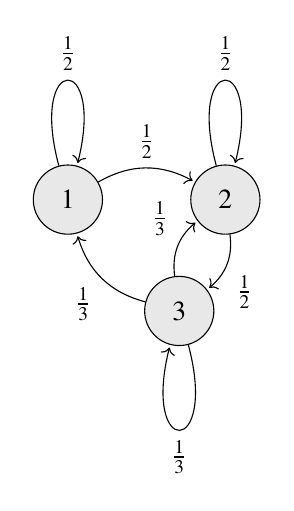
\begin{tikzpicture}[shorten >=1pt,node distance=2cm, scale =3, auto]
			\tikzstyle{every state}=[fill={rgb:black,1;white,10}]
			
			\node[state]   (q_1)                          {$1$};
			\node[state]   (q_2)  [right of=q_1]          {$2$};
			\node[state]   (q_3)  [below right of=q_1]          {$3$};
			
			\path[->]
			(q_1) edge [loop above] node {$\frac{1}{2}$}    (   )
			edge [bend left]  node {$\frac{1}{2}$}    (q_2)
			(q_2) edge [bend left]  node {$\frac{1}{2}$}    (q_3)
			edge [loop above] node {$\frac{1}{2}$}    ()
			(q_3) edge [bend left]  node {$\frac{1}{3}$}    (q_2)
			edge [bend left]  node {$\frac{1}{3}$}    (q_1)
			edge [loop below] node {$\frac{1}{3}$}    ();
		\end{tikzpicture}$
		
		\\  
		&\\
		&\\
		\hline
		\multirow{3}{*}{Checking whether the  } & \\
		& Here,\\chain is Irreducible
		& All the states are accessible to one another. \\and Aperiodic
		& $\implies$ They are in the same communication class. So, it is Irreducible.\\
		& \\
		& There exists the non- zero self-transition, which means that the chain \\
		& is Aperiodic.\\
		&\\ 
		& We know that if the Markov Chain is irreducible and aperiodic then \\
		& \qquad \qquad \qquad $\Vec{\pi}_{j} = \lim_{n \to \infty}P\{X_{n} = j\}$, $j = 1,...,N$ \\
		& These are the stationary probabilities. \\
		&\\
		\hline
		\multirow{3}{*}{Finding the Stationary} & \\
		& Stationary Probability can be represented as\\Probability Distributions
		& \qquad \qquad \qquad $\Vec{\pi} = \Vec{\pi} \vec{P}$\\
		& \\
		& \qquad $\implies$ $\myvec{v_{1}&&v_{2}&&v_{3}} = \myvec{v_{1}&&v_{2}&&v_{3}}\vec{P}$ \\
		& \\
		& Equating the above equation we get \\
		& \\
		& \qquad \qquad \qquad $\frac{1}{2}v_{1}-\frac{1}{3}v_{3} = 0$ $\label{eq:solutions/2018/dec/106/eq}$\\
		& \\
		& \qquad \qquad \qquad $\frac{1}{2}v_{1}-\frac{1}{2}v_{2} + \frac{1}{3}v_{3} = 0$\\
		& \\
		& \qquad \qquad \qquad $\frac{1}{2}v_{2}-\frac{2}{3}v_{3} = 0$\\
		& \\\
		& We see that summation of second and the third equation gives us the \\
		& first equation only. \\
		& And we know that the probability distribution will sum up to 1. \\
		& \\
		& \qquad \qquad \qquad $v_{1}+v_{2}+v_{3} = 1$ \\
		& \\
		& Therefore, we get the equation form as \\
		& \\
		& \qquad \qquad \qquad $\myvec{1&1&1\\\frac{1}{2}&0&\frac{-1}{3}\\\frac{1}{2}&\frac{-1}{2}&\frac{1}{3}}\myvec{v_{1}\\v_{2}\\v_{3}} = \myvec{1\\0\\0}$ \\
		& \\
		\hline
		\multirow{3}{*}{Solving the linear} & \\
		& The above linear equation can be solved using Gauss-Jordan method as\\equtions
		& \\
		& \qquad \qquad \qquad $\myvec{1&1&1&\vrule&1\\\frac{1}{2}&0&\frac{-1}{3}&\vrule&0\\\frac{1}{2}&\frac{-1}{2}&\frac{1}{3}&\vrule&0}$\\
		& \\
		& \qquad $\xleftrightarrow[]{R_2 \leftarrow R_2 - \frac{1}{2}R_1}$
		$\myvec{1&1&1&\vrule&1\\0&\frac{-1}{2}&\frac{-5}{6}&\vrule&\frac{-1}{2}\\\frac{1}{2}&\frac{-1}{2}&\frac{1}{3}&\vrule&0}$\\
		&\\
		& \qquad $\xleftrightarrow[]{R_3 \leftarrow R_3 - \frac{1}{2}R_1}$
		$\myvec{1&1&1&\vrule&1\\0&\frac{-1}{2}&\frac{-5}{6}&\vrule&\frac{-1}{2}\\0&-1&\frac{-1}{6}&\vrule&\frac{-1}{2}}$\\
		&\\
		& \qquad $\xleftrightarrow[]{R_2 \leftarrow \frac{-1}{2}R_2}$
		$\myvec{1&1&1&\vrule&1\\0&1&\frac{5}{3}&\vrule&1\\0&-1&\frac{-1}{6}&\vrule&\frac{-1}{2}}$\\
		&\\
		& \qquad $\xleftrightarrow[]{R_3 \leftarrow R_3 + R_2}$
		$\myvec{1&1&1&\vrule&1\\0&1&\frac{5}{3}&\vrule&1\\0&0&\frac{3}{2}&\vrule&\frac{1}{2}}$\\
		&\\
		& \qquad $\xleftrightarrow[]{R_3 \leftarrow \frac{3}{2}R_3}$
		$\myvec{1&1&1&\vrule&1\\0&1&\frac{5}{3}&\vrule&1\\0&0&1&\vrule&\frac{1}{3}}$\\
		&\\
		& \qquad $\xleftrightarrow[]{R_2 \leftarrow R_2 - \frac{5}{3}R_3}$
		$\myvec{1&1&1&\vrule&1\\0&1&0&\vrule&\frac{4}{9}\\0&0&1&\vrule&\frac{1}{3}}$\\
		&\\
		& \qquad $\xleftrightarrow[]{R_1 \leftarrow R_1 - R_3}$
		$\myvec{1&1&0&\vrule&\frac{2}{3}\\0&1&0&\vrule&\frac{4}{9}\\0&0&1&\vrule&\frac{1}{3}}$\\
		&\\
		& \qquad $\xleftrightarrow[]{R_1 \leftarrow R_1 - R_2}$
		$\myvec{1&0&0&\vrule&\frac{2}{9}\\0&1&0&\vrule&\frac{4}{9}\\0&0&1&\vrule&\frac{1}{3}}$\\
		&\\
		& $\therefore$, stationary probability distribution $\pi$ is given by \\
		& \qquad \qquad $\pi = \myvec{\frac{2}{9} & \frac{4}{9} & \frac{1}{3}}$ \\
		& \\
		\hline
		\multirow{3}{*}{Observations} & \\
		
		
		& Since the given transition probability matrix $\vec{P}$ is irreducible and aperiodic, \\
		& then $\lim_{n \to \infty} \vec{P}^{n}$ converges to a matrix with all rows identical and equal to $\vec{\pi}$. \\
		& \\
		& We were able to find $\vec{\pi}$ as $\myvec{\frac{2}{9} & \frac{4}{9} & \frac{1}{3}}$ \\
		& \\
		& $\lim_{n \to \infty} \vec{P}^{n} = \myvec{\frac{2}{9}&\frac{4}{9}&\frac{1}{3}\\\frac{2}{9}&\frac{4}{9}&\frac{1}{3}\\\frac{2}{9}&\frac{4}{9}&\frac{1}{3}}$\\
		& \\
		& From the above matrix, we get \\
		& \\
		& $\lim_{n \to \infty} \vec{P}^{n}_{11} = \frac{2}{9}$ \\
		&\\
		& $\lim_{n \to \infty} \vec{P}^{n}_{21} = \frac{2}{9}$ \\
		&\\
		& $\lim_{n \to \infty} \vec{P}^{n}_{32} = \frac{4}{9}$ \\
		&\\
		& $\lim_{n \to \infty} \vec{P}^{n}_{13} = \frac{1}{3}$ \\
		&\\
		\hline
		\multirow{3}{*}{Conclusion} & \\
		& From our observation we see that \\
		&\\
		& Options 1) and 4) are True.\\
		& \\
		\hline
\caption{}
\label{eq:solutions/2018/dec/106/table1}
	\end{longtable}
\twocolumn

\item Which of the following matrices is not diagonalizable over $\mathbb{R}$?
\begin{enumerate}
\begin{multicols}{2}
\item $\myvec{2 & 0 & 1 \\ 0 & 3 & 0 \\ 0 & 0 & 2}$
\item $\myvec{1 & 1 \\ 1 & 1}$
\item $\myvec{2 & 0 & 1 \\ 0 & 3 & 0 \\ 0 & 0 & 3}$
\item $\myvec{1 & -1 \\ 2 & 4}$
\end{multicols}
\end{enumerate}
\item What is the rank of the following matrix?
\begin{align}
\myvec
{
1 & 1 & 1 & 1 & 1 \\
1 & 2 & 2 & 2 & 2 \\
1 & 2 & 3 & 3 & 3 \\
1 & 2 & 3 & 4 & 4 \\
1 & 2 & 3 & 4 & 5 
}
\end{align}
\item Let $V$ denote the vector space of real valued continuous functions on the close interval $\sbrak{0,1}$.  Let $W$ be the subspace of $V$ spanned by $\cbrak{\sin x, \cos x, \tan x}$.  Find the dimension of $W$ over $\mathbb{R}$.
\solution
See Tables \ref{eq:solutions/2018/dec/106/table0} and \ref{eq:solutions/2018/dec/106/table1}


\onecolumn
	\begin{longtable}{|l|l|}
		\hline
		\multirow{3}{*}{Irreducible Markov Chain} 
		& \\
		& A Markov chain is $\textbf{irreducible}$ if all the states communicate with each other,\\
		& i.e., if there is only one communication class.\\
		&\\
		\hline
		\multirow{3}{*}{Aperiodic Markov Chain} & \\
		& If there is a self-transition in the chain ($p^{ii}>0$ for some i), then the chain is\\
		& called as $\textbf{aperiodic}$\\
		& \\
		\hline
		\multirow{3}{*}{Stationary Distribution} & \\
		& A stationary distribution of a Markov chain is a probability distribution that\\
		& remains unchanged in the Markov chain as time progresses. Typically, it is\\
		& represented as a row vector $\Vec{\pi}$ whose entries are probabilities summing to 1,\\ 
		& and given transition matrix $\textbf{P}$, it satisfies\\
		& \\
		&  \qquad \qquad  \qquad$\Vec{\pi} = \Vec{\pi} \textbf{P}$\\
		& \\
		\hline
\caption{}
\label{eq:solutions/2018/dec/106/table0}
	\end{longtable}
	\begin{longtable}{|l|l|}
		\hline
		\multirow{3}{*}{Drawing Transition diagram} 
		& \\
		& 
		
		$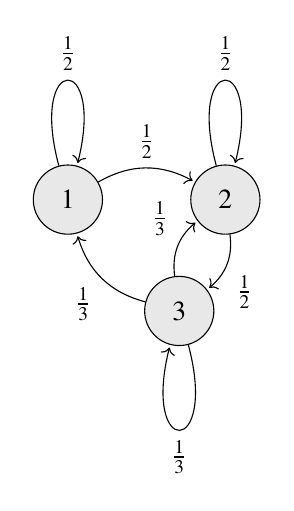
\begin{tikzpicture}[shorten >=1pt,node distance=2cm, scale =3, auto]
			\tikzstyle{every state}=[fill={rgb:black,1;white,10}]
			
			\node[state]   (q_1)                          {$1$};
			\node[state]   (q_2)  [right of=q_1]          {$2$};
			\node[state]   (q_3)  [below right of=q_1]          {$3$};
			
			\path[->]
			(q_1) edge [loop above] node {$\frac{1}{2}$}    (   )
			edge [bend left]  node {$\frac{1}{2}$}    (q_2)
			(q_2) edge [bend left]  node {$\frac{1}{2}$}    (q_3)
			edge [loop above] node {$\frac{1}{2}$}    ()
			(q_3) edge [bend left]  node {$\frac{1}{3}$}    (q_2)
			edge [bend left]  node {$\frac{1}{3}$}    (q_1)
			edge [loop below] node {$\frac{1}{3}$}    ();
		\end{tikzpicture}$
		
		\\  
		&\\
		&\\
		\hline
		\multirow{3}{*}{Checking whether the  } & \\
		& Here,\\chain is Irreducible
		& All the states are accessible to one another. \\and Aperiodic
		& $\implies$ They are in the same communication class. So, it is Irreducible.\\
		& \\
		& There exists the non- zero self-transition, which means that the chain \\
		& is Aperiodic.\\
		&\\ 
		& We know that if the Markov Chain is irreducible and aperiodic then \\
		& \qquad \qquad \qquad $\Vec{\pi}_{j} = \lim_{n \to \infty}P\{X_{n} = j\}$, $j = 1,...,N$ \\
		& These are the stationary probabilities. \\
		&\\
		\hline
		\multirow{3}{*}{Finding the Stationary} & \\
		& Stationary Probability can be represented as\\Probability Distributions
		& \qquad \qquad \qquad $\Vec{\pi} = \Vec{\pi} \vec{P}$\\
		& \\
		& \qquad $\implies$ $\myvec{v_{1}&&v_{2}&&v_{3}} = \myvec{v_{1}&&v_{2}&&v_{3}}\vec{P}$ \\
		& \\
		& Equating the above equation we get \\
		& \\
		& \qquad \qquad \qquad $\frac{1}{2}v_{1}-\frac{1}{3}v_{3} = 0$ $\label{eq:solutions/2018/dec/106/eq}$\\
		& \\
		& \qquad \qquad \qquad $\frac{1}{2}v_{1}-\frac{1}{2}v_{2} + \frac{1}{3}v_{3} = 0$\\
		& \\
		& \qquad \qquad \qquad $\frac{1}{2}v_{2}-\frac{2}{3}v_{3} = 0$\\
		& \\\
		& We see that summation of second and the third equation gives us the \\
		& first equation only. \\
		& And we know that the probability distribution will sum up to 1. \\
		& \\
		& \qquad \qquad \qquad $v_{1}+v_{2}+v_{3} = 1$ \\
		& \\
		& Therefore, we get the equation form as \\
		& \\
		& \qquad \qquad \qquad $\myvec{1&1&1\\\frac{1}{2}&0&\frac{-1}{3}\\\frac{1}{2}&\frac{-1}{2}&\frac{1}{3}}\myvec{v_{1}\\v_{2}\\v_{3}} = \myvec{1\\0\\0}$ \\
		& \\
		\hline
		\multirow{3}{*}{Solving the linear} & \\
		& The above linear equation can be solved using Gauss-Jordan method as\\equtions
		& \\
		& \qquad \qquad \qquad $\myvec{1&1&1&\vrule&1\\\frac{1}{2}&0&\frac{-1}{3}&\vrule&0\\\frac{1}{2}&\frac{-1}{2}&\frac{1}{3}&\vrule&0}$\\
		& \\
		& \qquad $\xleftrightarrow[]{R_2 \leftarrow R_2 - \frac{1}{2}R_1}$
		$\myvec{1&1&1&\vrule&1\\0&\frac{-1}{2}&\frac{-5}{6}&\vrule&\frac{-1}{2}\\\frac{1}{2}&\frac{-1}{2}&\frac{1}{3}&\vrule&0}$\\
		&\\
		& \qquad $\xleftrightarrow[]{R_3 \leftarrow R_3 - \frac{1}{2}R_1}$
		$\myvec{1&1&1&\vrule&1\\0&\frac{-1}{2}&\frac{-5}{6}&\vrule&\frac{-1}{2}\\0&-1&\frac{-1}{6}&\vrule&\frac{-1}{2}}$\\
		&\\
		& \qquad $\xleftrightarrow[]{R_2 \leftarrow \frac{-1}{2}R_2}$
		$\myvec{1&1&1&\vrule&1\\0&1&\frac{5}{3}&\vrule&1\\0&-1&\frac{-1}{6}&\vrule&\frac{-1}{2}}$\\
		&\\
		& \qquad $\xleftrightarrow[]{R_3 \leftarrow R_3 + R_2}$
		$\myvec{1&1&1&\vrule&1\\0&1&\frac{5}{3}&\vrule&1\\0&0&\frac{3}{2}&\vrule&\frac{1}{2}}$\\
		&\\
		& \qquad $\xleftrightarrow[]{R_3 \leftarrow \frac{3}{2}R_3}$
		$\myvec{1&1&1&\vrule&1\\0&1&\frac{5}{3}&\vrule&1\\0&0&1&\vrule&\frac{1}{3}}$\\
		&\\
		& \qquad $\xleftrightarrow[]{R_2 \leftarrow R_2 - \frac{5}{3}R_3}$
		$\myvec{1&1&1&\vrule&1\\0&1&0&\vrule&\frac{4}{9}\\0&0&1&\vrule&\frac{1}{3}}$\\
		&\\
		& \qquad $\xleftrightarrow[]{R_1 \leftarrow R_1 - R_3}$
		$\myvec{1&1&0&\vrule&\frac{2}{3}\\0&1&0&\vrule&\frac{4}{9}\\0&0&1&\vrule&\frac{1}{3}}$\\
		&\\
		& \qquad $\xleftrightarrow[]{R_1 \leftarrow R_1 - R_2}$
		$\myvec{1&0&0&\vrule&\frac{2}{9}\\0&1&0&\vrule&\frac{4}{9}\\0&0&1&\vrule&\frac{1}{3}}$\\
		&\\
		& $\therefore$, stationary probability distribution $\pi$ is given by \\
		& \qquad \qquad $\pi = \myvec{\frac{2}{9} & \frac{4}{9} & \frac{1}{3}}$ \\
		& \\
		\hline
		\multirow{3}{*}{Observations} & \\
		
		
		& Since the given transition probability matrix $\vec{P}$ is irreducible and aperiodic, \\
		& then $\lim_{n \to \infty} \vec{P}^{n}$ converges to a matrix with all rows identical and equal to $\vec{\pi}$. \\
		& \\
		& We were able to find $\vec{\pi}$ as $\myvec{\frac{2}{9} & \frac{4}{9} & \frac{1}{3}}$ \\
		& \\
		& $\lim_{n \to \infty} \vec{P}^{n} = \myvec{\frac{2}{9}&\frac{4}{9}&\frac{1}{3}\\\frac{2}{9}&\frac{4}{9}&\frac{1}{3}\\\frac{2}{9}&\frac{4}{9}&\frac{1}{3}}$\\
		& \\
		& From the above matrix, we get \\
		& \\
		& $\lim_{n \to \infty} \vec{P}^{n}_{11} = \frac{2}{9}$ \\
		&\\
		& $\lim_{n \to \infty} \vec{P}^{n}_{21} = \frac{2}{9}$ \\
		&\\
		& $\lim_{n \to \infty} \vec{P}^{n}_{32} = \frac{4}{9}$ \\
		&\\
		& $\lim_{n \to \infty} \vec{P}^{n}_{13} = \frac{1}{3}$ \\
		&\\
		\hline
		\multirow{3}{*}{Conclusion} & \\
		& From our observation we see that \\
		&\\
		& Options 1) and 4) are True.\\
		& \\
		\hline
\caption{}
\label{eq:solutions/2018/dec/106/table1}
	\end{longtable}
\twocolumn


\item Let $V$ be the vector space of polynomials in the variable $t$ of degree at most 2 over $\mathbb{R}$.  An inner product on $V$ is defined by
\begin{align}
f^Tg = \int_{0}^{1}f(t)g(t)\,dt, \quad f,g \in V.
\end{align}
Let
\begin{align}
W = span\cbrak{1-t^2,1+t^2}
\end{align}
and $W^{\perp}$  be the orthogonal complement of $W$ in $V$.  Which of the following conditions is satisfied for all $h \in W^{\perp}$?
\begin{enumerate}
\item $h$ is an even function
\item $h$ is an odd function
\item $h(t) =0$ has a real solution
\item $h(0) = 0$
\end{enumerate}
\item Consider solving the following system by Jacobi iteration scheme
\begin{align}
\myvec
{
1 & 2m & -2m \\
n & 1 & n \\
2m & 2m & 1
}
\myvec{x}
= \myvec{ 1 \\ 2 \\1}
\end{align}
where $m,n \in \mathbb{Z}$.  With any initial vector, the scheme converges provided $m,n$ satisfy
\begin{enumerate}
\begin{multicols}{2}
\item $m+n = 3$
\item $m > n$
\item $m < n$
\item $m = n$
\end{multicols}
\end{enumerate}
\item Consider a Markov Chain with state space $\cbrak{0,1,2,3,4}$ and transition matrix
\begin{align}
P = 
%\begin{blockarray}{c@{\hspace{1pt}}rrr@{\hspace{3pt}}}
%         & 0   & 1   & 2 \\
%        \begin{block}{r@{\hspace{3pt}}@{\hspace{1pt}}
%    (@{\hspace{1pt}}rrr@{\hspace{1pt}}@{\hspace{1pt}})}
%        0 & 0.7 & 0.2 & 0.1 \\
%        1 & 0.3 & 0.5 & 0.2 \\
%        2 & 0   & 0   & 0   \\
%        \end{block}
%    \end{blockarray}
\begin{blockarray}{c@{\hspace{1pt}}rrrrr@{\hspace{3pt}}}
         & 0   & 1   & 2 &3 & 4\\
        \begin{block}{r@{\hspace{3pt}}@{\hspace{1pt}}
    (@{\hspace{1pt}}rrrrr@{\hspace{1pt}}@{\hspace{1pt}})}
        0 & 1 & 0 & 0 & 0 & 0 \\
        1 & \frac{1}{3} & \frac{1}{3} & \frac{1}{3} & 0 & 0 \\
%
        2 & 0 & \frac{1}{3} & \frac{1}{3} & \frac{1}{3} & 0  \\
        3 & 0 & 0 & \frac{1}{3} & \frac{1}{3} & \frac{1}{3}   \\
        4 & 0 & 0 & 0 & 0 & 1 \\
        \end{block}
    \end{blockarray}
\end{align}
Then find 
\begin{align}
\lim_{n \to \infty} p_{23}^{\brak{n}}
\end{align}
\item Let $L\brak{\mathbb{R}}^n$ be the space of $\mathbb{R}-$linear maps from $\mathbb{R}^n$ to $\mathbb{R}^n$.  If $Ker(T)$ denotes the kernel of $T$ then which of the following are true?
\begin{enumerate}
\item There exists $T \in L\brak{\mathbb{R}^5}\ \cbrak{0}$ such that $Range(T) = Ker(T)$
\item There does not exist $T \in L\brak{\mathbb{R}^5}\ \cbrak{0}$ such that $Range(T) = Ker(T)$
\item There exists $T \in L\brak{\mathbb{R}^6}\ \cbrak{0}$ such that $Range(T) = Ker(T)$
\item There does not exist $T \in L\brak{\mathbb{R}^6}\ \cbrak{0}$ such that $Range(T) = Ker(T)$
\end{enumerate}
\item Let $V$ be a finite dimensional vector space over $\mathbb{R}$ and $T:V\to V$ be a linear map.   Can you always write $T = T_2 \circ T_1$ for some linear maps
\begin{align}
T_1:V\to W, T:W\to V,
\end{align}
where $W$ is some finite dimensional vector space such that\begin{enumerate}
\item both $T_1$ and $T_2$ are onto
\item both $T_1$ and $T_2$ are one to one
\item $T_1$ is onto, $T_2$ is one to one
\item $T_1$ is one to one, $T_2$ is onto
\end{enumerate}
\item Let $A = \sbrak{a_{ij}}$ be a $3\times 3$ complex matrix.  Identify the correct statements
\begin{enumerate}
\item $det\sbrak{\brak{-1}^{i+j}a_{ij}} = det(A)$
\item $det\sbrak{\brak{-1}^{i+j}a_{ij}} = -det(A)$
\item $det\sbrak{\brak{\sqrt{-1}}^{i+j}a_{ij}} = det(A)$
\item $det\sbrak{\brak{\sqrt{-1}}^{i+j}a_{ij}} = -det(A)$
\end{enumerate}
\item Let 
\begin{align}
p(x) = a_0 + a_1x + \dots + a_n x^n 
\end{align}
be a non-constant polynomial of degree $n \ge 1$.  Consider the polynomial
\begin{align}
q(x) = \int_{0}^{x}p(t)\, dt,
r(x) = \frac{d}{dx}p(x)
\end{align}
Let $V$ denote the real vector space of all polynomials in $x$.  Then which of the following are true?
\begin{enumerate}
\item $q$ and $r$ are linearly independent in $V$
\item $q$ and $r$ are linearly dependent in $V$
\item $x^n$ belongs to the linear span of $q$ and $r$
\item $x^{n+1}$ belongs to the linear span of $q$ and $r$.
\end{enumerate}
\item Let $M_n\brak{\mathbb{R}}$ be the ring of $n \times n$ matrices over $\mathbb{R}$.  Which of the following are true for every $n \ge 2$?
\begin{enumerate}
\item there exist matrices $A,B \in M_n\brak{\mathbb{R}}$ such that $AB- BA = I_n$, where $I_n$ denotes the identity matrix.
\item If $A,B \in M_n\brak{\mathbb{R}}$ and $AB = BA$, then $A$ is diagonalisable over $\mathbb{R}$ if and only if $B$ is diagonalisable over $\mathbb{R}$.
\item If $A,B \in M_n\brak{\mathbb{R}}$, then $AB$ and $BA$ have the same minimal polynomial.
\item If $A,B \in M_n\brak{\mathbb{R}}$, then $AB$ and $BA$ have the same eigenvalues in $\mathbb{R}$.
\end{enumerate}
\solution
See Tables \ref{eq:solutions/2018/dec/106/table0} and \ref{eq:solutions/2018/dec/106/table1}


\onecolumn
	\begin{longtable}{|l|l|}
		\hline
		\multirow{3}{*}{Irreducible Markov Chain} 
		& \\
		& A Markov chain is $\textbf{irreducible}$ if all the states communicate with each other,\\
		& i.e., if there is only one communication class.\\
		&\\
		\hline
		\multirow{3}{*}{Aperiodic Markov Chain} & \\
		& If there is a self-transition in the chain ($p^{ii}>0$ for some i), then the chain is\\
		& called as $\textbf{aperiodic}$\\
		& \\
		\hline
		\multirow{3}{*}{Stationary Distribution} & \\
		& A stationary distribution of a Markov chain is a probability distribution that\\
		& remains unchanged in the Markov chain as time progresses. Typically, it is\\
		& represented as a row vector $\Vec{\pi}$ whose entries are probabilities summing to 1,\\ 
		& and given transition matrix $\textbf{P}$, it satisfies\\
		& \\
		&  \qquad \qquad  \qquad$\Vec{\pi} = \Vec{\pi} \textbf{P}$\\
		& \\
		\hline
\caption{}
\label{eq:solutions/2018/dec/106/table0}
	\end{longtable}
	\begin{longtable}{|l|l|}
		\hline
		\multirow{3}{*}{Drawing Transition diagram} 
		& \\
		& 
		
		$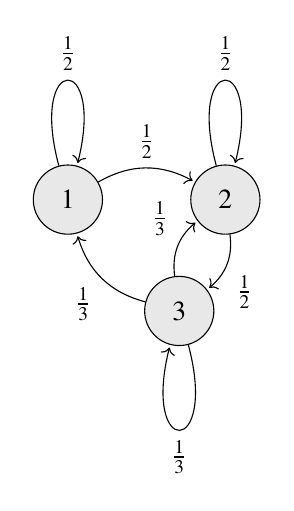
\begin{tikzpicture}[shorten >=1pt,node distance=2cm, scale =3, auto]
			\tikzstyle{every state}=[fill={rgb:black,1;white,10}]
			
			\node[state]   (q_1)                          {$1$};
			\node[state]   (q_2)  [right of=q_1]          {$2$};
			\node[state]   (q_3)  [below right of=q_1]          {$3$};
			
			\path[->]
			(q_1) edge [loop above] node {$\frac{1}{2}$}    (   )
			edge [bend left]  node {$\frac{1}{2}$}    (q_2)
			(q_2) edge [bend left]  node {$\frac{1}{2}$}    (q_3)
			edge [loop above] node {$\frac{1}{2}$}    ()
			(q_3) edge [bend left]  node {$\frac{1}{3}$}    (q_2)
			edge [bend left]  node {$\frac{1}{3}$}    (q_1)
			edge [loop below] node {$\frac{1}{3}$}    ();
		\end{tikzpicture}$
		
		\\  
		&\\
		&\\
		\hline
		\multirow{3}{*}{Checking whether the  } & \\
		& Here,\\chain is Irreducible
		& All the states are accessible to one another. \\and Aperiodic
		& $\implies$ They are in the same communication class. So, it is Irreducible.\\
		& \\
		& There exists the non- zero self-transition, which means that the chain \\
		& is Aperiodic.\\
		&\\ 
		& We know that if the Markov Chain is irreducible and aperiodic then \\
		& \qquad \qquad \qquad $\Vec{\pi}_{j} = \lim_{n \to \infty}P\{X_{n} = j\}$, $j = 1,...,N$ \\
		& These are the stationary probabilities. \\
		&\\
		\hline
		\multirow{3}{*}{Finding the Stationary} & \\
		& Stationary Probability can be represented as\\Probability Distributions
		& \qquad \qquad \qquad $\Vec{\pi} = \Vec{\pi} \vec{P}$\\
		& \\
		& \qquad $\implies$ $\myvec{v_{1}&&v_{2}&&v_{3}} = \myvec{v_{1}&&v_{2}&&v_{3}}\vec{P}$ \\
		& \\
		& Equating the above equation we get \\
		& \\
		& \qquad \qquad \qquad $\frac{1}{2}v_{1}-\frac{1}{3}v_{3} = 0$ $\label{eq:solutions/2018/dec/106/eq}$\\
		& \\
		& \qquad \qquad \qquad $\frac{1}{2}v_{1}-\frac{1}{2}v_{2} + \frac{1}{3}v_{3} = 0$\\
		& \\
		& \qquad \qquad \qquad $\frac{1}{2}v_{2}-\frac{2}{3}v_{3} = 0$\\
		& \\\
		& We see that summation of second and the third equation gives us the \\
		& first equation only. \\
		& And we know that the probability distribution will sum up to 1. \\
		& \\
		& \qquad \qquad \qquad $v_{1}+v_{2}+v_{3} = 1$ \\
		& \\
		& Therefore, we get the equation form as \\
		& \\
		& \qquad \qquad \qquad $\myvec{1&1&1\\\frac{1}{2}&0&\frac{-1}{3}\\\frac{1}{2}&\frac{-1}{2}&\frac{1}{3}}\myvec{v_{1}\\v_{2}\\v_{3}} = \myvec{1\\0\\0}$ \\
		& \\
		\hline
		\multirow{3}{*}{Solving the linear} & \\
		& The above linear equation can be solved using Gauss-Jordan method as\\equtions
		& \\
		& \qquad \qquad \qquad $\myvec{1&1&1&\vrule&1\\\frac{1}{2}&0&\frac{-1}{3}&\vrule&0\\\frac{1}{2}&\frac{-1}{2}&\frac{1}{3}&\vrule&0}$\\
		& \\
		& \qquad $\xleftrightarrow[]{R_2 \leftarrow R_2 - \frac{1}{2}R_1}$
		$\myvec{1&1&1&\vrule&1\\0&\frac{-1}{2}&\frac{-5}{6}&\vrule&\frac{-1}{2}\\\frac{1}{2}&\frac{-1}{2}&\frac{1}{3}&\vrule&0}$\\
		&\\
		& \qquad $\xleftrightarrow[]{R_3 \leftarrow R_3 - \frac{1}{2}R_1}$
		$\myvec{1&1&1&\vrule&1\\0&\frac{-1}{2}&\frac{-5}{6}&\vrule&\frac{-1}{2}\\0&-1&\frac{-1}{6}&\vrule&\frac{-1}{2}}$\\
		&\\
		& \qquad $\xleftrightarrow[]{R_2 \leftarrow \frac{-1}{2}R_2}$
		$\myvec{1&1&1&\vrule&1\\0&1&\frac{5}{3}&\vrule&1\\0&-1&\frac{-1}{6}&\vrule&\frac{-1}{2}}$\\
		&\\
		& \qquad $\xleftrightarrow[]{R_3 \leftarrow R_3 + R_2}$
		$\myvec{1&1&1&\vrule&1\\0&1&\frac{5}{3}&\vrule&1\\0&0&\frac{3}{2}&\vrule&\frac{1}{2}}$\\
		&\\
		& \qquad $\xleftrightarrow[]{R_3 \leftarrow \frac{3}{2}R_3}$
		$\myvec{1&1&1&\vrule&1\\0&1&\frac{5}{3}&\vrule&1\\0&0&1&\vrule&\frac{1}{3}}$\\
		&\\
		& \qquad $\xleftrightarrow[]{R_2 \leftarrow R_2 - \frac{5}{3}R_3}$
		$\myvec{1&1&1&\vrule&1\\0&1&0&\vrule&\frac{4}{9}\\0&0&1&\vrule&\frac{1}{3}}$\\
		&\\
		& \qquad $\xleftrightarrow[]{R_1 \leftarrow R_1 - R_3}$
		$\myvec{1&1&0&\vrule&\frac{2}{3}\\0&1&0&\vrule&\frac{4}{9}\\0&0&1&\vrule&\frac{1}{3}}$\\
		&\\
		& \qquad $\xleftrightarrow[]{R_1 \leftarrow R_1 - R_2}$
		$\myvec{1&0&0&\vrule&\frac{2}{9}\\0&1&0&\vrule&\frac{4}{9}\\0&0&1&\vrule&\frac{1}{3}}$\\
		&\\
		& $\therefore$, stationary probability distribution $\pi$ is given by \\
		& \qquad \qquad $\pi = \myvec{\frac{2}{9} & \frac{4}{9} & \frac{1}{3}}$ \\
		& \\
		\hline
		\multirow{3}{*}{Observations} & \\
		
		
		& Since the given transition probability matrix $\vec{P}$ is irreducible and aperiodic, \\
		& then $\lim_{n \to \infty} \vec{P}^{n}$ converges to a matrix with all rows identical and equal to $\vec{\pi}$. \\
		& \\
		& We were able to find $\vec{\pi}$ as $\myvec{\frac{2}{9} & \frac{4}{9} & \frac{1}{3}}$ \\
		& \\
		& $\lim_{n \to \infty} \vec{P}^{n} = \myvec{\frac{2}{9}&\frac{4}{9}&\frac{1}{3}\\\frac{2}{9}&\frac{4}{9}&\frac{1}{3}\\\frac{2}{9}&\frac{4}{9}&\frac{1}{3}}$\\
		& \\
		& From the above matrix, we get \\
		& \\
		& $\lim_{n \to \infty} \vec{P}^{n}_{11} = \frac{2}{9}$ \\
		&\\
		& $\lim_{n \to \infty} \vec{P}^{n}_{21} = \frac{2}{9}$ \\
		&\\
		& $\lim_{n \to \infty} \vec{P}^{n}_{32} = \frac{4}{9}$ \\
		&\\
		& $\lim_{n \to \infty} \vec{P}^{n}_{13} = \frac{1}{3}$ \\
		&\\
		\hline
		\multirow{3}{*}{Conclusion} & \\
		& From our observation we see that \\
		&\\
		& Options 1) and 4) are True.\\
		& \\
		\hline
\caption{}
\label{eq:solutions/2018/dec/106/table1}
	\end{longtable}
\twocolumn

\item Consider a matrix 
\begin{align}
A = \sbrak{a_{ij}}, 1 \le i,j \le 5
\end{align}
such that
\begin{align}
a_{ij} = \frac{1}{n_i+n_j+1}, \quad n_i,n_j \in \mathbb{N}
\end{align}
Then in which of the following cases $A$ is a positive definite matrix?
\begin{enumerate}
\item $n_i = 1 \forall i = 1,2,3,4,5$.
\item $n_1 < n_2 < \dots < n_5$.
\item $n_1 = n_2 = \dots = n_5$.
\item $n_1 > n_2 > \dots > n_5$.
\end{enumerate}
\item For a nonzero $w \in \mathbb{R}^n$, define
\begin{align}
T_w: \mathbb{R}^n \to \mathbb{R}^n
\end{align}
by
\begin{align}
T_w = v - \frac{2v^Tw}{w^Tw}w, \quad v \in \mathbb{R}^n
\end{align}
Which of the following are true?
\begin{enumerate}
\item $det\brak{T_w} = 1$
\item $T_w(v_1)^T_w(v_2) = v_1^Tv_2 \forall v_1, v_2 \in \mathbb{R}^n$
\item  $T_w = T_w ^{-1}$
\item  $T_{2w} = 2T_{w}$
\end{enumerate}
\item Consider the matrix 
\begin{align}
A = \myvec{0 & 1 \\ 1 & 0}
\end{align}
over the field $\mathbb{Q}$ of rationals.  Which of the following matrices are of the form $P^TAP$ for suitable $2\times 2$ invertible matrix $P$ over $\mathbb{Q}$?
\begin{enumerate}
\begin{multicols}{2}
\item $\myvec{2 & 0 \\ 0 & -2}$
\item $\myvec{2 & 0 \\ 0 & 2}$
\item $\myvec{1 & 0 \\ 0 & -1}$
\item $\myvec{3 & 4 \\ 4 & 5}$
\end{multicols}
\end{enumerate}
\item Consider a Markov Chain with state space $\cbrak{0,1,2}$ and transition matrix
\begin{align}
P = 
\begin{blockarray}{c@{\hspace{1pt}}rrr@{\hspace{3pt}}}
         & 0   & 1   & 2 \\
        \begin{block}{r@{\hspace{3pt}}@{\hspace{1pt}}
    (@{\hspace{1pt}}rrr@{\hspace{1pt}}@{\hspace{1pt}})}
        0 & \frac{1}{4} & \frac{5}{8} & \frac{1}{8}  \\[1mm]
        1 & \frac{1}{4} & 0 & \frac{3}{4}  \\[1mm]
        2 &  \frac{1}{2} & \frac{3}{8} & \frac{1}{8}  \\
        \end{block}
    \end{blockarray}
\end{align}
Then which of the following are true?
\begin{enumerate}
\item $\lim_{n \to \infty} p_{12}^{(n)} = 0$
\item $\lim_{n \to \infty} p_{12}^{(n)} = \lim_{n \to \infty} p_{21}^{(n)}$
\item $\lim_{n \to \infty} p_{22}^{(n)} = \frac{1}{8}$
\item $\lim_{n \to \infty} p_{21}^{(n)} = \frac{1}{3}$
\end{enumerate}
\end{enumerate}


\section{December 2018}
\renewcommand{\theequation}{\theenumi}
\renewcommand{\thefigure}{\theenumi}
\begin{enumerate}[label=\thesection.\arabic*.,ref=\thesection.\theenumi]
\numberwithin{equation}{enumi}
\numberwithin{figure}{enumi}
\numberwithin{table}{enumi}

\item Consider the subspaces $W_1$ and $W_2$ of $\mathbb{R}^3$ given by
\begin{align}
W_1 &= \cbrak{\vec{x} \in \mathbb{R}^3: \myvec{1 & 1 & 1}\vec{x} = 0}
\label{eq:solutions/2018/dec/27/eq:1}
\\
W_2 &= \cbrak{\vec{x} \in \mathbb{R}^3: \myvec{1 & -1 & 1}\vec{x} = 0}.
\label{eq:solutions/2018/dec/27/eq:2}
\end{align}
If $W \subseteq \mathbb{R}^3$, such that 
\begin{enumerate}
\item $W \cap W_2 =$ span $\cbrak{\myvec{0\\1\\1}}$
\label{eq:solutions/2018/dec/27/eq:3}
\item $\cbrak{W \cap W_1} \perp \cbrak{W \cap W_2}$, 
\label{eq:solutions/2018/dec/27/eq:4}
\end{enumerate}
then 
\begin{enumerate}
\item $W =$ span $\cbrak{\myvec{0\\1\\-1},\myvec{0\\1\\1}}$
\item $W =$ span $\cbrak{\myvec{1\\0\\-1},\myvec{0\\1\\-1}}$
\item $W =$ span $\cbrak{\myvec{1\\0\\-1},\myvec{0\\1\\1}}$
\item $W =$ span $\cbrak{\myvec{1\\0\\-1},\myvec{1\\0\\1}}$
\end{enumerate}
\solution
See Tables \ref{eq:solutions/2018/dec/106/table0} and \ref{eq:solutions/2018/dec/106/table1}


\onecolumn
	\begin{longtable}{|l|l|}
		\hline
		\multirow{3}{*}{Irreducible Markov Chain} 
		& \\
		& A Markov chain is $\textbf{irreducible}$ if all the states communicate with each other,\\
		& i.e., if there is only one communication class.\\
		&\\
		\hline
		\multirow{3}{*}{Aperiodic Markov Chain} & \\
		& If there is a self-transition in the chain ($p^{ii}>0$ for some i), then the chain is\\
		& called as $\textbf{aperiodic}$\\
		& \\
		\hline
		\multirow{3}{*}{Stationary Distribution} & \\
		& A stationary distribution of a Markov chain is a probability distribution that\\
		& remains unchanged in the Markov chain as time progresses. Typically, it is\\
		& represented as a row vector $\Vec{\pi}$ whose entries are probabilities summing to 1,\\ 
		& and given transition matrix $\textbf{P}$, it satisfies\\
		& \\
		&  \qquad \qquad  \qquad$\Vec{\pi} = \Vec{\pi} \textbf{P}$\\
		& \\
		\hline
\caption{}
\label{eq:solutions/2018/dec/106/table0}
	\end{longtable}
	\begin{longtable}{|l|l|}
		\hline
		\multirow{3}{*}{Drawing Transition diagram} 
		& \\
		& 
		
		$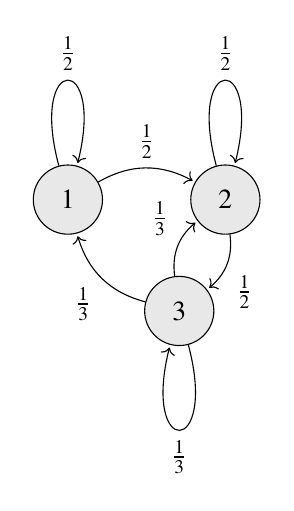
\begin{tikzpicture}[shorten >=1pt,node distance=2cm, scale =3, auto]
			\tikzstyle{every state}=[fill={rgb:black,1;white,10}]
			
			\node[state]   (q_1)                          {$1$};
			\node[state]   (q_2)  [right of=q_1]          {$2$};
			\node[state]   (q_3)  [below right of=q_1]          {$3$};
			
			\path[->]
			(q_1) edge [loop above] node {$\frac{1}{2}$}    (   )
			edge [bend left]  node {$\frac{1}{2}$}    (q_2)
			(q_2) edge [bend left]  node {$\frac{1}{2}$}    (q_3)
			edge [loop above] node {$\frac{1}{2}$}    ()
			(q_3) edge [bend left]  node {$\frac{1}{3}$}    (q_2)
			edge [bend left]  node {$\frac{1}{3}$}    (q_1)
			edge [loop below] node {$\frac{1}{3}$}    ();
		\end{tikzpicture}$
		
		\\  
		&\\
		&\\
		\hline
		\multirow{3}{*}{Checking whether the  } & \\
		& Here,\\chain is Irreducible
		& All the states are accessible to one another. \\and Aperiodic
		& $\implies$ They are in the same communication class. So, it is Irreducible.\\
		& \\
		& There exists the non- zero self-transition, which means that the chain \\
		& is Aperiodic.\\
		&\\ 
		& We know that if the Markov Chain is irreducible and aperiodic then \\
		& \qquad \qquad \qquad $\Vec{\pi}_{j} = \lim_{n \to \infty}P\{X_{n} = j\}$, $j = 1,...,N$ \\
		& These are the stationary probabilities. \\
		&\\
		\hline
		\multirow{3}{*}{Finding the Stationary} & \\
		& Stationary Probability can be represented as\\Probability Distributions
		& \qquad \qquad \qquad $\Vec{\pi} = \Vec{\pi} \vec{P}$\\
		& \\
		& \qquad $\implies$ $\myvec{v_{1}&&v_{2}&&v_{3}} = \myvec{v_{1}&&v_{2}&&v_{3}}\vec{P}$ \\
		& \\
		& Equating the above equation we get \\
		& \\
		& \qquad \qquad \qquad $\frac{1}{2}v_{1}-\frac{1}{3}v_{3} = 0$ $\label{eq:solutions/2018/dec/106/eq}$\\
		& \\
		& \qquad \qquad \qquad $\frac{1}{2}v_{1}-\frac{1}{2}v_{2} + \frac{1}{3}v_{3} = 0$\\
		& \\
		& \qquad \qquad \qquad $\frac{1}{2}v_{2}-\frac{2}{3}v_{3} = 0$\\
		& \\\
		& We see that summation of second and the third equation gives us the \\
		& first equation only. \\
		& And we know that the probability distribution will sum up to 1. \\
		& \\
		& \qquad \qquad \qquad $v_{1}+v_{2}+v_{3} = 1$ \\
		& \\
		& Therefore, we get the equation form as \\
		& \\
		& \qquad \qquad \qquad $\myvec{1&1&1\\\frac{1}{2}&0&\frac{-1}{3}\\\frac{1}{2}&\frac{-1}{2}&\frac{1}{3}}\myvec{v_{1}\\v_{2}\\v_{3}} = \myvec{1\\0\\0}$ \\
		& \\
		\hline
		\multirow{3}{*}{Solving the linear} & \\
		& The above linear equation can be solved using Gauss-Jordan method as\\equtions
		& \\
		& \qquad \qquad \qquad $\myvec{1&1&1&\vrule&1\\\frac{1}{2}&0&\frac{-1}{3}&\vrule&0\\\frac{1}{2}&\frac{-1}{2}&\frac{1}{3}&\vrule&0}$\\
		& \\
		& \qquad $\xleftrightarrow[]{R_2 \leftarrow R_2 - \frac{1}{2}R_1}$
		$\myvec{1&1&1&\vrule&1\\0&\frac{-1}{2}&\frac{-5}{6}&\vrule&\frac{-1}{2}\\\frac{1}{2}&\frac{-1}{2}&\frac{1}{3}&\vrule&0}$\\
		&\\
		& \qquad $\xleftrightarrow[]{R_3 \leftarrow R_3 - \frac{1}{2}R_1}$
		$\myvec{1&1&1&\vrule&1\\0&\frac{-1}{2}&\frac{-5}{6}&\vrule&\frac{-1}{2}\\0&-1&\frac{-1}{6}&\vrule&\frac{-1}{2}}$\\
		&\\
		& \qquad $\xleftrightarrow[]{R_2 \leftarrow \frac{-1}{2}R_2}$
		$\myvec{1&1&1&\vrule&1\\0&1&\frac{5}{3}&\vrule&1\\0&-1&\frac{-1}{6}&\vrule&\frac{-1}{2}}$\\
		&\\
		& \qquad $\xleftrightarrow[]{R_3 \leftarrow R_3 + R_2}$
		$\myvec{1&1&1&\vrule&1\\0&1&\frac{5}{3}&\vrule&1\\0&0&\frac{3}{2}&\vrule&\frac{1}{2}}$\\
		&\\
		& \qquad $\xleftrightarrow[]{R_3 \leftarrow \frac{3}{2}R_3}$
		$\myvec{1&1&1&\vrule&1\\0&1&\frac{5}{3}&\vrule&1\\0&0&1&\vrule&\frac{1}{3}}$\\
		&\\
		& \qquad $\xleftrightarrow[]{R_2 \leftarrow R_2 - \frac{5}{3}R_3}$
		$\myvec{1&1&1&\vrule&1\\0&1&0&\vrule&\frac{4}{9}\\0&0&1&\vrule&\frac{1}{3}}$\\
		&\\
		& \qquad $\xleftrightarrow[]{R_1 \leftarrow R_1 - R_3}$
		$\myvec{1&1&0&\vrule&\frac{2}{3}\\0&1&0&\vrule&\frac{4}{9}\\0&0&1&\vrule&\frac{1}{3}}$\\
		&\\
		& \qquad $\xleftrightarrow[]{R_1 \leftarrow R_1 - R_2}$
		$\myvec{1&0&0&\vrule&\frac{2}{9}\\0&1&0&\vrule&\frac{4}{9}\\0&0&1&\vrule&\frac{1}{3}}$\\
		&\\
		& $\therefore$, stationary probability distribution $\pi$ is given by \\
		& \qquad \qquad $\pi = \myvec{\frac{2}{9} & \frac{4}{9} & \frac{1}{3}}$ \\
		& \\
		\hline
		\multirow{3}{*}{Observations} & \\
		
		
		& Since the given transition probability matrix $\vec{P}$ is irreducible and aperiodic, \\
		& then $\lim_{n \to \infty} \vec{P}^{n}$ converges to a matrix with all rows identical and equal to $\vec{\pi}$. \\
		& \\
		& We were able to find $\vec{\pi}$ as $\myvec{\frac{2}{9} & \frac{4}{9} & \frac{1}{3}}$ \\
		& \\
		& $\lim_{n \to \infty} \vec{P}^{n} = \myvec{\frac{2}{9}&\frac{4}{9}&\frac{1}{3}\\\frac{2}{9}&\frac{4}{9}&\frac{1}{3}\\\frac{2}{9}&\frac{4}{9}&\frac{1}{3}}$\\
		& \\
		& From the above matrix, we get \\
		& \\
		& $\lim_{n \to \infty} \vec{P}^{n}_{11} = \frac{2}{9}$ \\
		&\\
		& $\lim_{n \to \infty} \vec{P}^{n}_{21} = \frac{2}{9}$ \\
		&\\
		& $\lim_{n \to \infty} \vec{P}^{n}_{32} = \frac{4}{9}$ \\
		&\\
		& $\lim_{n \to \infty} \vec{P}^{n}_{13} = \frac{1}{3}$ \\
		&\\
		\hline
		\multirow{3}{*}{Conclusion} & \\
		& From our observation we see that \\
		&\\
		& Options 1) and 4) are True.\\
		& \\
		\hline
\caption{}
\label{eq:solutions/2018/dec/106/table1}
	\end{longtable}
\twocolumn

%
\item Let
\begin{align}
C = \cbrak{\myvec{1 \\ 2},\myvec{2 \\ 1}}
\end{align}
be a basis of $\mathbb{R}^2$ and 
\begin{align}
T\myvec{x\\y} = \myvec{x+y \\ x-2y}.
\end{align}
If $T\sbrak{C}$ represents the matrix of $T$ with respect to the basis C then
which among the following is true?
\begin{enumerate}
\item $T\sbrak{C} = \myvec{-3 & -2\\3 & 1}$
\item $T\sbrak{C} = \myvec{3 & -2\\-3 & 1}$
\item $T\sbrak{C} = \myvec{-3 & -1\\3 & 2}$
\item $T\sbrak{C} = \myvec{3 & -1\\-3 & 2}$
\end{enumerate}
\solution
See Tables \ref{eq:solutions/2018/dec/106/table0} and \ref{eq:solutions/2018/dec/106/table1}


\onecolumn
	\begin{longtable}{|l|l|}
		\hline
		\multirow{3}{*}{Irreducible Markov Chain} 
		& \\
		& A Markov chain is $\textbf{irreducible}$ if all the states communicate with each other,\\
		& i.e., if there is only one communication class.\\
		&\\
		\hline
		\multirow{3}{*}{Aperiodic Markov Chain} & \\
		& If there is a self-transition in the chain ($p^{ii}>0$ for some i), then the chain is\\
		& called as $\textbf{aperiodic}$\\
		& \\
		\hline
		\multirow{3}{*}{Stationary Distribution} & \\
		& A stationary distribution of a Markov chain is a probability distribution that\\
		& remains unchanged in the Markov chain as time progresses. Typically, it is\\
		& represented as a row vector $\Vec{\pi}$ whose entries are probabilities summing to 1,\\ 
		& and given transition matrix $\textbf{P}$, it satisfies\\
		& \\
		&  \qquad \qquad  \qquad$\Vec{\pi} = \Vec{\pi} \textbf{P}$\\
		& \\
		\hline
\caption{}
\label{eq:solutions/2018/dec/106/table0}
	\end{longtable}
	\begin{longtable}{|l|l|}
		\hline
		\multirow{3}{*}{Drawing Transition diagram} 
		& \\
		& 
		
		$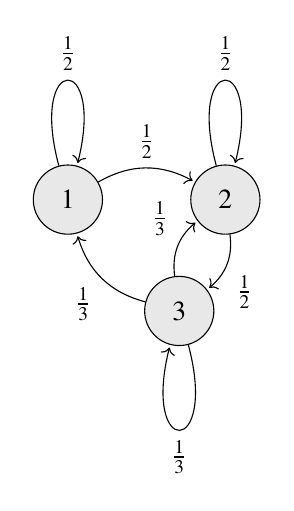
\begin{tikzpicture}[shorten >=1pt,node distance=2cm, scale =3, auto]
			\tikzstyle{every state}=[fill={rgb:black,1;white,10}]
			
			\node[state]   (q_1)                          {$1$};
			\node[state]   (q_2)  [right of=q_1]          {$2$};
			\node[state]   (q_3)  [below right of=q_1]          {$3$};
			
			\path[->]
			(q_1) edge [loop above] node {$\frac{1}{2}$}    (   )
			edge [bend left]  node {$\frac{1}{2}$}    (q_2)
			(q_2) edge [bend left]  node {$\frac{1}{2}$}    (q_3)
			edge [loop above] node {$\frac{1}{2}$}    ()
			(q_3) edge [bend left]  node {$\frac{1}{3}$}    (q_2)
			edge [bend left]  node {$\frac{1}{3}$}    (q_1)
			edge [loop below] node {$\frac{1}{3}$}    ();
		\end{tikzpicture}$
		
		\\  
		&\\
		&\\
		\hline
		\multirow{3}{*}{Checking whether the  } & \\
		& Here,\\chain is Irreducible
		& All the states are accessible to one another. \\and Aperiodic
		& $\implies$ They are in the same communication class. So, it is Irreducible.\\
		& \\
		& There exists the non- zero self-transition, which means that the chain \\
		& is Aperiodic.\\
		&\\ 
		& We know that if the Markov Chain is irreducible and aperiodic then \\
		& \qquad \qquad \qquad $\Vec{\pi}_{j} = \lim_{n \to \infty}P\{X_{n} = j\}$, $j = 1,...,N$ \\
		& These are the stationary probabilities. \\
		&\\
		\hline
		\multirow{3}{*}{Finding the Stationary} & \\
		& Stationary Probability can be represented as\\Probability Distributions
		& \qquad \qquad \qquad $\Vec{\pi} = \Vec{\pi} \vec{P}$\\
		& \\
		& \qquad $\implies$ $\myvec{v_{1}&&v_{2}&&v_{3}} = \myvec{v_{1}&&v_{2}&&v_{3}}\vec{P}$ \\
		& \\
		& Equating the above equation we get \\
		& \\
		& \qquad \qquad \qquad $\frac{1}{2}v_{1}-\frac{1}{3}v_{3} = 0$ $\label{eq:solutions/2018/dec/106/eq}$\\
		& \\
		& \qquad \qquad \qquad $\frac{1}{2}v_{1}-\frac{1}{2}v_{2} + \frac{1}{3}v_{3} = 0$\\
		& \\
		& \qquad \qquad \qquad $\frac{1}{2}v_{2}-\frac{2}{3}v_{3} = 0$\\
		& \\\
		& We see that summation of second and the third equation gives us the \\
		& first equation only. \\
		& And we know that the probability distribution will sum up to 1. \\
		& \\
		& \qquad \qquad \qquad $v_{1}+v_{2}+v_{3} = 1$ \\
		& \\
		& Therefore, we get the equation form as \\
		& \\
		& \qquad \qquad \qquad $\myvec{1&1&1\\\frac{1}{2}&0&\frac{-1}{3}\\\frac{1}{2}&\frac{-1}{2}&\frac{1}{3}}\myvec{v_{1}\\v_{2}\\v_{3}} = \myvec{1\\0\\0}$ \\
		& \\
		\hline
		\multirow{3}{*}{Solving the linear} & \\
		& The above linear equation can be solved using Gauss-Jordan method as\\equtions
		& \\
		& \qquad \qquad \qquad $\myvec{1&1&1&\vrule&1\\\frac{1}{2}&0&\frac{-1}{3}&\vrule&0\\\frac{1}{2}&\frac{-1}{2}&\frac{1}{3}&\vrule&0}$\\
		& \\
		& \qquad $\xleftrightarrow[]{R_2 \leftarrow R_2 - \frac{1}{2}R_1}$
		$\myvec{1&1&1&\vrule&1\\0&\frac{-1}{2}&\frac{-5}{6}&\vrule&\frac{-1}{2}\\\frac{1}{2}&\frac{-1}{2}&\frac{1}{3}&\vrule&0}$\\
		&\\
		& \qquad $\xleftrightarrow[]{R_3 \leftarrow R_3 - \frac{1}{2}R_1}$
		$\myvec{1&1&1&\vrule&1\\0&\frac{-1}{2}&\frac{-5}{6}&\vrule&\frac{-1}{2}\\0&-1&\frac{-1}{6}&\vrule&\frac{-1}{2}}$\\
		&\\
		& \qquad $\xleftrightarrow[]{R_2 \leftarrow \frac{-1}{2}R_2}$
		$\myvec{1&1&1&\vrule&1\\0&1&\frac{5}{3}&\vrule&1\\0&-1&\frac{-1}{6}&\vrule&\frac{-1}{2}}$\\
		&\\
		& \qquad $\xleftrightarrow[]{R_3 \leftarrow R_3 + R_2}$
		$\myvec{1&1&1&\vrule&1\\0&1&\frac{5}{3}&\vrule&1\\0&0&\frac{3}{2}&\vrule&\frac{1}{2}}$\\
		&\\
		& \qquad $\xleftrightarrow[]{R_3 \leftarrow \frac{3}{2}R_3}$
		$\myvec{1&1&1&\vrule&1\\0&1&\frac{5}{3}&\vrule&1\\0&0&1&\vrule&\frac{1}{3}}$\\
		&\\
		& \qquad $\xleftrightarrow[]{R_2 \leftarrow R_2 - \frac{5}{3}R_3}$
		$\myvec{1&1&1&\vrule&1\\0&1&0&\vrule&\frac{4}{9}\\0&0&1&\vrule&\frac{1}{3}}$\\
		&\\
		& \qquad $\xleftrightarrow[]{R_1 \leftarrow R_1 - R_3}$
		$\myvec{1&1&0&\vrule&\frac{2}{3}\\0&1&0&\vrule&\frac{4}{9}\\0&0&1&\vrule&\frac{1}{3}}$\\
		&\\
		& \qquad $\xleftrightarrow[]{R_1 \leftarrow R_1 - R_2}$
		$\myvec{1&0&0&\vrule&\frac{2}{9}\\0&1&0&\vrule&\frac{4}{9}\\0&0&1&\vrule&\frac{1}{3}}$\\
		&\\
		& $\therefore$, stationary probability distribution $\pi$ is given by \\
		& \qquad \qquad $\pi = \myvec{\frac{2}{9} & \frac{4}{9} & \frac{1}{3}}$ \\
		& \\
		\hline
		\multirow{3}{*}{Observations} & \\
		
		
		& Since the given transition probability matrix $\vec{P}$ is irreducible and aperiodic, \\
		& then $\lim_{n \to \infty} \vec{P}^{n}$ converges to a matrix with all rows identical and equal to $\vec{\pi}$. \\
		& \\
		& We were able to find $\vec{\pi}$ as $\myvec{\frac{2}{9} & \frac{4}{9} & \frac{1}{3}}$ \\
		& \\
		& $\lim_{n \to \infty} \vec{P}^{n} = \myvec{\frac{2}{9}&\frac{4}{9}&\frac{1}{3}\\\frac{2}{9}&\frac{4}{9}&\frac{1}{3}\\\frac{2}{9}&\frac{4}{9}&\frac{1}{3}}$\\
		& \\
		& From the above matrix, we get \\
		& \\
		& $\lim_{n \to \infty} \vec{P}^{n}_{11} = \frac{2}{9}$ \\
		&\\
		& $\lim_{n \to \infty} \vec{P}^{n}_{21} = \frac{2}{9}$ \\
		&\\
		& $\lim_{n \to \infty} \vec{P}^{n}_{32} = \frac{4}{9}$ \\
		&\\
		& $\lim_{n \to \infty} \vec{P}^{n}_{13} = \frac{1}{3}$ \\
		&\\
		\hline
		\multirow{3}{*}{Conclusion} & \\
		& From our observation we see that \\
		&\\
		& Options 1) and 4) are True.\\
		& \\
		\hline
\caption{}
\label{eq:solutions/2018/dec/106/table1}
	\end{longtable}
\twocolumn

\item Let $W_1 = \cbrak{\vec{x} \in \mathbb{R}^4:}$
\begin{align}
 \myvec{1 & 1 & 1 & 0}\vec{x} = 0
\\
 \myvec{0 & 2 & 0 & 1}\vec{x} = 0
\\
 \myvec{2 & 0 & 2 & -1}\vec{x} = 0
\end{align}
and
$W_2 = \cbrak{\vec{x} \in \mathbb{R}^4:}$
\begin{align}
 \myvec{1 & 1 & 0 & 1}\vec{x} &= 0
\\
 \myvec{1 & 0 & 1 & -2}\vec{x} &= 0
\\
 \myvec{0 & 1 & 0 & -1}\vec{x} &= 0.
\end{align}
Then which among the following is true?
\begin{enumerate}
\item $\text{dim}\brak{W_1} = 1$
\item $\text{dim}\brak{W_2} = 2$
\item $\text{dim}\brak{W_1 \cap W_2} = 1$
\item $\text{dim}\brak{W_1+W_2} = 3$
\end{enumerate}
%
\item Let $A$ be an $n \times n$ complex matrix.  Assume that $A$ is self-adjoint and let $B$ denote the inverse of $A + \j I$. Then all eigenvalues of $\brak{A-\j I}B$ are 
\begin{enumerate}
\item purely imaginary
\item of modulus one
\item real
\item of modulus less than one
\end{enumerate}  
%
\item Let $\cbrak{u_1,u_2,\dots, u_n}$ be an orthonormal basis of $\mathbb{C}^n$ as column vectors.Let 
\begin{align}
\vec{M} &= \myvec{\vec{u}_1 & \vec{u}_2 & \dots & \vec{u}_k},
\\
\vec{N} &= \myvec{\vec{u}_{k+1} & \vec{u}_{k+2} & \dots & \vec{u}_n}
\end{align}
%
and $\vec{P}$ be the diagonal $k \times k$ matrix with diagonal entries $\alpha_1,\alpha_2, \dots, \alpha_k \in \mathbb{R}$.  Then which of the following is true?
\begin{enumerate}
\item rank$\brak{\vec{M}\vec{P}\vec{M}^*} = k$ whenever $\alpha_i \ne \alpha_j, 1 \le i, j \le k$.
\item tr$\brak{\vec{M}\vec{P}\vec{M}^*} = \sum_{i=1}^{k}\alpha_i$
\item rank$\brak{\vec{M}^*\vec{N}} = \min\brak{k,n-k}$
\item rank$\brak{\vec{M}\vec{M}^*+\vec{N}\vec{N}^*}  < n$.
\end{enumerate}  
%
\solution
See Tables \ref{eq:solutions/2018/dec/106/table0} and \ref{eq:solutions/2018/dec/106/table1}


\onecolumn
	\begin{longtable}{|l|l|}
		\hline
		\multirow{3}{*}{Irreducible Markov Chain} 
		& \\
		& A Markov chain is $\textbf{irreducible}$ if all the states communicate with each other,\\
		& i.e., if there is only one communication class.\\
		&\\
		\hline
		\multirow{3}{*}{Aperiodic Markov Chain} & \\
		& If there is a self-transition in the chain ($p^{ii}>0$ for some i), then the chain is\\
		& called as $\textbf{aperiodic}$\\
		& \\
		\hline
		\multirow{3}{*}{Stationary Distribution} & \\
		& A stationary distribution of a Markov chain is a probability distribution that\\
		& remains unchanged in the Markov chain as time progresses. Typically, it is\\
		& represented as a row vector $\Vec{\pi}$ whose entries are probabilities summing to 1,\\ 
		& and given transition matrix $\textbf{P}$, it satisfies\\
		& \\
		&  \qquad \qquad  \qquad$\Vec{\pi} = \Vec{\pi} \textbf{P}$\\
		& \\
		\hline
\caption{}
\label{eq:solutions/2018/dec/106/table0}
	\end{longtable}
	\begin{longtable}{|l|l|}
		\hline
		\multirow{3}{*}{Drawing Transition diagram} 
		& \\
		& 
		
		$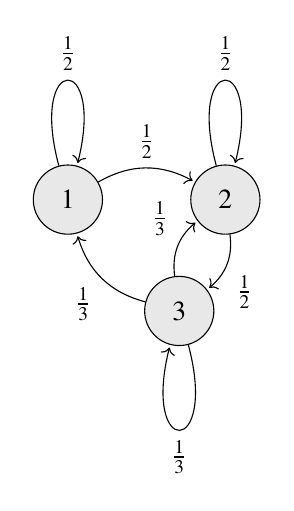
\begin{tikzpicture}[shorten >=1pt,node distance=2cm, scale =3, auto]
			\tikzstyle{every state}=[fill={rgb:black,1;white,10}]
			
			\node[state]   (q_1)                          {$1$};
			\node[state]   (q_2)  [right of=q_1]          {$2$};
			\node[state]   (q_3)  [below right of=q_1]          {$3$};
			
			\path[->]
			(q_1) edge [loop above] node {$\frac{1}{2}$}    (   )
			edge [bend left]  node {$\frac{1}{2}$}    (q_2)
			(q_2) edge [bend left]  node {$\frac{1}{2}$}    (q_3)
			edge [loop above] node {$\frac{1}{2}$}    ()
			(q_3) edge [bend left]  node {$\frac{1}{3}$}    (q_2)
			edge [bend left]  node {$\frac{1}{3}$}    (q_1)
			edge [loop below] node {$\frac{1}{3}$}    ();
		\end{tikzpicture}$
		
		\\  
		&\\
		&\\
		\hline
		\multirow{3}{*}{Checking whether the  } & \\
		& Here,\\chain is Irreducible
		& All the states are accessible to one another. \\and Aperiodic
		& $\implies$ They are in the same communication class. So, it is Irreducible.\\
		& \\
		& There exists the non- zero self-transition, which means that the chain \\
		& is Aperiodic.\\
		&\\ 
		& We know that if the Markov Chain is irreducible and aperiodic then \\
		& \qquad \qquad \qquad $\Vec{\pi}_{j} = \lim_{n \to \infty}P\{X_{n} = j\}$, $j = 1,...,N$ \\
		& These are the stationary probabilities. \\
		&\\
		\hline
		\multirow{3}{*}{Finding the Stationary} & \\
		& Stationary Probability can be represented as\\Probability Distributions
		& \qquad \qquad \qquad $\Vec{\pi} = \Vec{\pi} \vec{P}$\\
		& \\
		& \qquad $\implies$ $\myvec{v_{1}&&v_{2}&&v_{3}} = \myvec{v_{1}&&v_{2}&&v_{3}}\vec{P}$ \\
		& \\
		& Equating the above equation we get \\
		& \\
		& \qquad \qquad \qquad $\frac{1}{2}v_{1}-\frac{1}{3}v_{3} = 0$ $\label{eq:solutions/2018/dec/106/eq}$\\
		& \\
		& \qquad \qquad \qquad $\frac{1}{2}v_{1}-\frac{1}{2}v_{2} + \frac{1}{3}v_{3} = 0$\\
		& \\
		& \qquad \qquad \qquad $\frac{1}{2}v_{2}-\frac{2}{3}v_{3} = 0$\\
		& \\\
		& We see that summation of second and the third equation gives us the \\
		& first equation only. \\
		& And we know that the probability distribution will sum up to 1. \\
		& \\
		& \qquad \qquad \qquad $v_{1}+v_{2}+v_{3} = 1$ \\
		& \\
		& Therefore, we get the equation form as \\
		& \\
		& \qquad \qquad \qquad $\myvec{1&1&1\\\frac{1}{2}&0&\frac{-1}{3}\\\frac{1}{2}&\frac{-1}{2}&\frac{1}{3}}\myvec{v_{1}\\v_{2}\\v_{3}} = \myvec{1\\0\\0}$ \\
		& \\
		\hline
		\multirow{3}{*}{Solving the linear} & \\
		& The above linear equation can be solved using Gauss-Jordan method as\\equtions
		& \\
		& \qquad \qquad \qquad $\myvec{1&1&1&\vrule&1\\\frac{1}{2}&0&\frac{-1}{3}&\vrule&0\\\frac{1}{2}&\frac{-1}{2}&\frac{1}{3}&\vrule&0}$\\
		& \\
		& \qquad $\xleftrightarrow[]{R_2 \leftarrow R_2 - \frac{1}{2}R_1}$
		$\myvec{1&1&1&\vrule&1\\0&\frac{-1}{2}&\frac{-5}{6}&\vrule&\frac{-1}{2}\\\frac{1}{2}&\frac{-1}{2}&\frac{1}{3}&\vrule&0}$\\
		&\\
		& \qquad $\xleftrightarrow[]{R_3 \leftarrow R_3 - \frac{1}{2}R_1}$
		$\myvec{1&1&1&\vrule&1\\0&\frac{-1}{2}&\frac{-5}{6}&\vrule&\frac{-1}{2}\\0&-1&\frac{-1}{6}&\vrule&\frac{-1}{2}}$\\
		&\\
		& \qquad $\xleftrightarrow[]{R_2 \leftarrow \frac{-1}{2}R_2}$
		$\myvec{1&1&1&\vrule&1\\0&1&\frac{5}{3}&\vrule&1\\0&-1&\frac{-1}{6}&\vrule&\frac{-1}{2}}$\\
		&\\
		& \qquad $\xleftrightarrow[]{R_3 \leftarrow R_3 + R_2}$
		$\myvec{1&1&1&\vrule&1\\0&1&\frac{5}{3}&\vrule&1\\0&0&\frac{3}{2}&\vrule&\frac{1}{2}}$\\
		&\\
		& \qquad $\xleftrightarrow[]{R_3 \leftarrow \frac{3}{2}R_3}$
		$\myvec{1&1&1&\vrule&1\\0&1&\frac{5}{3}&\vrule&1\\0&0&1&\vrule&\frac{1}{3}}$\\
		&\\
		& \qquad $\xleftrightarrow[]{R_2 \leftarrow R_2 - \frac{5}{3}R_3}$
		$\myvec{1&1&1&\vrule&1\\0&1&0&\vrule&\frac{4}{9}\\0&0&1&\vrule&\frac{1}{3}}$\\
		&\\
		& \qquad $\xleftrightarrow[]{R_1 \leftarrow R_1 - R_3}$
		$\myvec{1&1&0&\vrule&\frac{2}{3}\\0&1&0&\vrule&\frac{4}{9}\\0&0&1&\vrule&\frac{1}{3}}$\\
		&\\
		& \qquad $\xleftrightarrow[]{R_1 \leftarrow R_1 - R_2}$
		$\myvec{1&0&0&\vrule&\frac{2}{9}\\0&1&0&\vrule&\frac{4}{9}\\0&0&1&\vrule&\frac{1}{3}}$\\
		&\\
		& $\therefore$, stationary probability distribution $\pi$ is given by \\
		& \qquad \qquad $\pi = \myvec{\frac{2}{9} & \frac{4}{9} & \frac{1}{3}}$ \\
		& \\
		\hline
		\multirow{3}{*}{Observations} & \\
		
		
		& Since the given transition probability matrix $\vec{P}$ is irreducible and aperiodic, \\
		& then $\lim_{n \to \infty} \vec{P}^{n}$ converges to a matrix with all rows identical and equal to $\vec{\pi}$. \\
		& \\
		& We were able to find $\vec{\pi}$ as $\myvec{\frac{2}{9} & \frac{4}{9} & \frac{1}{3}}$ \\
		& \\
		& $\lim_{n \to \infty} \vec{P}^{n} = \myvec{\frac{2}{9}&\frac{4}{9}&\frac{1}{3}\\\frac{2}{9}&\frac{4}{9}&\frac{1}{3}\\\frac{2}{9}&\frac{4}{9}&\frac{1}{3}}$\\
		& \\
		& From the above matrix, we get \\
		& \\
		& $\lim_{n \to \infty} \vec{P}^{n}_{11} = \frac{2}{9}$ \\
		&\\
		& $\lim_{n \to \infty} \vec{P}^{n}_{21} = \frac{2}{9}$ \\
		&\\
		& $\lim_{n \to \infty} \vec{P}^{n}_{32} = \frac{4}{9}$ \\
		&\\
		& $\lim_{n \to \infty} \vec{P}^{n}_{13} = \frac{1}{3}$ \\
		&\\
		\hline
		\multirow{3}{*}{Conclusion} & \\
		& From our observation we see that \\
		&\\
		& Options 1) and 4) are True.\\
		& \\
		\hline
\caption{}
\label{eq:solutions/2018/dec/106/table1}
	\end{longtable}
\twocolumn

\item Let $B: \mathbb{R} \times \mathbb{R} \xrightarrow[]{} \mathbb{R}$ be the function $B(a,b) = ab$. Which of the following is true-
\begin{enumerate}
\item{$B$ is a linear transformation}
\item{$B$ is a positive definite bilinear form}
\item{$B$ is symmetric but not positive definite}
\item{$B$ neither linear nor bilinear}
\end{enumerate}
%
\solution
See Tables \ref{eq:solutions/2018/dec/106/table0} and \ref{eq:solutions/2018/dec/106/table1}


\onecolumn
	\begin{longtable}{|l|l|}
		\hline
		\multirow{3}{*}{Irreducible Markov Chain} 
		& \\
		& A Markov chain is $\textbf{irreducible}$ if all the states communicate with each other,\\
		& i.e., if there is only one communication class.\\
		&\\
		\hline
		\multirow{3}{*}{Aperiodic Markov Chain} & \\
		& If there is a self-transition in the chain ($p^{ii}>0$ for some i), then the chain is\\
		& called as $\textbf{aperiodic}$\\
		& \\
		\hline
		\multirow{3}{*}{Stationary Distribution} & \\
		& A stationary distribution of a Markov chain is a probability distribution that\\
		& remains unchanged in the Markov chain as time progresses. Typically, it is\\
		& represented as a row vector $\Vec{\pi}$ whose entries are probabilities summing to 1,\\ 
		& and given transition matrix $\textbf{P}$, it satisfies\\
		& \\
		&  \qquad \qquad  \qquad$\Vec{\pi} = \Vec{\pi} \textbf{P}$\\
		& \\
		\hline
\caption{}
\label{eq:solutions/2018/dec/106/table0}
	\end{longtable}
	\begin{longtable}{|l|l|}
		\hline
		\multirow{3}{*}{Drawing Transition diagram} 
		& \\
		& 
		
		$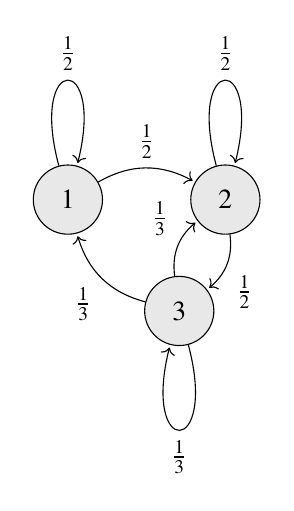
\begin{tikzpicture}[shorten >=1pt,node distance=2cm, scale =3, auto]
			\tikzstyle{every state}=[fill={rgb:black,1;white,10}]
			
			\node[state]   (q_1)                          {$1$};
			\node[state]   (q_2)  [right of=q_1]          {$2$};
			\node[state]   (q_3)  [below right of=q_1]          {$3$};
			
			\path[->]
			(q_1) edge [loop above] node {$\frac{1}{2}$}    (   )
			edge [bend left]  node {$\frac{1}{2}$}    (q_2)
			(q_2) edge [bend left]  node {$\frac{1}{2}$}    (q_3)
			edge [loop above] node {$\frac{1}{2}$}    ()
			(q_3) edge [bend left]  node {$\frac{1}{3}$}    (q_2)
			edge [bend left]  node {$\frac{1}{3}$}    (q_1)
			edge [loop below] node {$\frac{1}{3}$}    ();
		\end{tikzpicture}$
		
		\\  
		&\\
		&\\
		\hline
		\multirow{3}{*}{Checking whether the  } & \\
		& Here,\\chain is Irreducible
		& All the states are accessible to one another. \\and Aperiodic
		& $\implies$ They are in the same communication class. So, it is Irreducible.\\
		& \\
		& There exists the non- zero self-transition, which means that the chain \\
		& is Aperiodic.\\
		&\\ 
		& We know that if the Markov Chain is irreducible and aperiodic then \\
		& \qquad \qquad \qquad $\Vec{\pi}_{j} = \lim_{n \to \infty}P\{X_{n} = j\}$, $j = 1,...,N$ \\
		& These are the stationary probabilities. \\
		&\\
		\hline
		\multirow{3}{*}{Finding the Stationary} & \\
		& Stationary Probability can be represented as\\Probability Distributions
		& \qquad \qquad \qquad $\Vec{\pi} = \Vec{\pi} \vec{P}$\\
		& \\
		& \qquad $\implies$ $\myvec{v_{1}&&v_{2}&&v_{3}} = \myvec{v_{1}&&v_{2}&&v_{3}}\vec{P}$ \\
		& \\
		& Equating the above equation we get \\
		& \\
		& \qquad \qquad \qquad $\frac{1}{2}v_{1}-\frac{1}{3}v_{3} = 0$ $\label{eq:solutions/2018/dec/106/eq}$\\
		& \\
		& \qquad \qquad \qquad $\frac{1}{2}v_{1}-\frac{1}{2}v_{2} + \frac{1}{3}v_{3} = 0$\\
		& \\
		& \qquad \qquad \qquad $\frac{1}{2}v_{2}-\frac{2}{3}v_{3} = 0$\\
		& \\\
		& We see that summation of second and the third equation gives us the \\
		& first equation only. \\
		& And we know that the probability distribution will sum up to 1. \\
		& \\
		& \qquad \qquad \qquad $v_{1}+v_{2}+v_{3} = 1$ \\
		& \\
		& Therefore, we get the equation form as \\
		& \\
		& \qquad \qquad \qquad $\myvec{1&1&1\\\frac{1}{2}&0&\frac{-1}{3}\\\frac{1}{2}&\frac{-1}{2}&\frac{1}{3}}\myvec{v_{1}\\v_{2}\\v_{3}} = \myvec{1\\0\\0}$ \\
		& \\
		\hline
		\multirow{3}{*}{Solving the linear} & \\
		& The above linear equation can be solved using Gauss-Jordan method as\\equtions
		& \\
		& \qquad \qquad \qquad $\myvec{1&1&1&\vrule&1\\\frac{1}{2}&0&\frac{-1}{3}&\vrule&0\\\frac{1}{2}&\frac{-1}{2}&\frac{1}{3}&\vrule&0}$\\
		& \\
		& \qquad $\xleftrightarrow[]{R_2 \leftarrow R_2 - \frac{1}{2}R_1}$
		$\myvec{1&1&1&\vrule&1\\0&\frac{-1}{2}&\frac{-5}{6}&\vrule&\frac{-1}{2}\\\frac{1}{2}&\frac{-1}{2}&\frac{1}{3}&\vrule&0}$\\
		&\\
		& \qquad $\xleftrightarrow[]{R_3 \leftarrow R_3 - \frac{1}{2}R_1}$
		$\myvec{1&1&1&\vrule&1\\0&\frac{-1}{2}&\frac{-5}{6}&\vrule&\frac{-1}{2}\\0&-1&\frac{-1}{6}&\vrule&\frac{-1}{2}}$\\
		&\\
		& \qquad $\xleftrightarrow[]{R_2 \leftarrow \frac{-1}{2}R_2}$
		$\myvec{1&1&1&\vrule&1\\0&1&\frac{5}{3}&\vrule&1\\0&-1&\frac{-1}{6}&\vrule&\frac{-1}{2}}$\\
		&\\
		& \qquad $\xleftrightarrow[]{R_3 \leftarrow R_3 + R_2}$
		$\myvec{1&1&1&\vrule&1\\0&1&\frac{5}{3}&\vrule&1\\0&0&\frac{3}{2}&\vrule&\frac{1}{2}}$\\
		&\\
		& \qquad $\xleftrightarrow[]{R_3 \leftarrow \frac{3}{2}R_3}$
		$\myvec{1&1&1&\vrule&1\\0&1&\frac{5}{3}&\vrule&1\\0&0&1&\vrule&\frac{1}{3}}$\\
		&\\
		& \qquad $\xleftrightarrow[]{R_2 \leftarrow R_2 - \frac{5}{3}R_3}$
		$\myvec{1&1&1&\vrule&1\\0&1&0&\vrule&\frac{4}{9}\\0&0&1&\vrule&\frac{1}{3}}$\\
		&\\
		& \qquad $\xleftrightarrow[]{R_1 \leftarrow R_1 - R_3}$
		$\myvec{1&1&0&\vrule&\frac{2}{3}\\0&1&0&\vrule&\frac{4}{9}\\0&0&1&\vrule&\frac{1}{3}}$\\
		&\\
		& \qquad $\xleftrightarrow[]{R_1 \leftarrow R_1 - R_2}$
		$\myvec{1&0&0&\vrule&\frac{2}{9}\\0&1&0&\vrule&\frac{4}{9}\\0&0&1&\vrule&\frac{1}{3}}$\\
		&\\
		& $\therefore$, stationary probability distribution $\pi$ is given by \\
		& \qquad \qquad $\pi = \myvec{\frac{2}{9} & \frac{4}{9} & \frac{1}{3}}$ \\
		& \\
		\hline
		\multirow{3}{*}{Observations} & \\
		
		
		& Since the given transition probability matrix $\vec{P}$ is irreducible and aperiodic, \\
		& then $\lim_{n \to \infty} \vec{P}^{n}$ converges to a matrix with all rows identical and equal to $\vec{\pi}$. \\
		& \\
		& We were able to find $\vec{\pi}$ as $\myvec{\frac{2}{9} & \frac{4}{9} & \frac{1}{3}}$ \\
		& \\
		& $\lim_{n \to \infty} \vec{P}^{n} = \myvec{\frac{2}{9}&\frac{4}{9}&\frac{1}{3}\\\frac{2}{9}&\frac{4}{9}&\frac{1}{3}\\\frac{2}{9}&\frac{4}{9}&\frac{1}{3}}$\\
		& \\
		& From the above matrix, we get \\
		& \\
		& $\lim_{n \to \infty} \vec{P}^{n}_{11} = \frac{2}{9}$ \\
		&\\
		& $\lim_{n \to \infty} \vec{P}^{n}_{21} = \frac{2}{9}$ \\
		&\\
		& $\lim_{n \to \infty} \vec{P}^{n}_{32} = \frac{4}{9}$ \\
		&\\
		& $\lim_{n \to \infty} \vec{P}^{n}_{13} = \frac{1}{3}$ \\
		&\\
		\hline
		\multirow{3}{*}{Conclusion} & \\
		& From our observation we see that \\
		&\\
		& Options 1) and 4) are True.\\
		& \\
		\hline
\caption{}
\label{eq:solutions/2018/dec/106/table1}
	\end{longtable}
\twocolumn

\item Let $B: \mathbb{R} \times \mathbb{R} \to \mathbb{R}$ be the function
\begin{align}
B(a,b) = ab
\end{align}
Which of the following is true?
\begin{enumerate}
\item $B$ is a linear transformation
\item $B$ is a positive definite bilinear form
\item $B$ is symmetric but not positive definite
\item $B$ is neither linear nor bilinear
\end{enumerate}  
%
\item Let $\vec{A}$ be an invertible real $n \times n$ matrix.  Define a function
\begin{align}
F: \mathbb{R}^n \times \mathbb{R}^n \to \mathbb{R}
\end{align}
by 
\begin{align}
F(\vec{x},\vec{y}) = \brak{F\vec{x}}^T\vec{y}
\end{align}
Let $DF(\vec{x},\vec{y}) $ denote the derivate of $F$ at $(\vec{x},\vec{y}) $ which is 
a linear transformation from 
\begin{align}
\mathbb{R}^n \times \mathbb{R}^n \to \mathbb{R}
\end{align}
%
Then, if 
\begin{enumerate}
\item $\vec{x} \ne 0, DF(\vec{x},\vec{0}) \ne 0$ 
\item $\vec{y} \ne 0, DF(\vec{0},\vec{y}) \ne 0$ 
\item $(\vec{x},\vec{y}) \ne (\vec{0},\vec{0}), DF(\vec{x},\vec{0}) \ne 0$ 
\item $\vec{x} = 0$ or  $\vec{y} = 0, DF(\vec{x},\vec{y}) = 0$ 
\end{enumerate}  
%
\solution
See Tables \ref{eq:solutions/2018/dec/106/table0} and \ref{eq:solutions/2018/dec/106/table1}


\onecolumn
	\begin{longtable}{|l|l|}
		\hline
		\multirow{3}{*}{Irreducible Markov Chain} 
		& \\
		& A Markov chain is $\textbf{irreducible}$ if all the states communicate with each other,\\
		& i.e., if there is only one communication class.\\
		&\\
		\hline
		\multirow{3}{*}{Aperiodic Markov Chain} & \\
		& If there is a self-transition in the chain ($p^{ii}>0$ for some i), then the chain is\\
		& called as $\textbf{aperiodic}$\\
		& \\
		\hline
		\multirow{3}{*}{Stationary Distribution} & \\
		& A stationary distribution of a Markov chain is a probability distribution that\\
		& remains unchanged in the Markov chain as time progresses. Typically, it is\\
		& represented as a row vector $\Vec{\pi}$ whose entries are probabilities summing to 1,\\ 
		& and given transition matrix $\textbf{P}$, it satisfies\\
		& \\
		&  \qquad \qquad  \qquad$\Vec{\pi} = \Vec{\pi} \textbf{P}$\\
		& \\
		\hline
\caption{}
\label{eq:solutions/2018/dec/106/table0}
	\end{longtable}
	\begin{longtable}{|l|l|}
		\hline
		\multirow{3}{*}{Drawing Transition diagram} 
		& \\
		& 
		
		$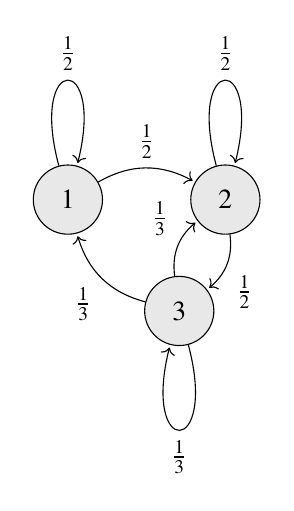
\begin{tikzpicture}[shorten >=1pt,node distance=2cm, scale =3, auto]
			\tikzstyle{every state}=[fill={rgb:black,1;white,10}]
			
			\node[state]   (q_1)                          {$1$};
			\node[state]   (q_2)  [right of=q_1]          {$2$};
			\node[state]   (q_3)  [below right of=q_1]          {$3$};
			
			\path[->]
			(q_1) edge [loop above] node {$\frac{1}{2}$}    (   )
			edge [bend left]  node {$\frac{1}{2}$}    (q_2)
			(q_2) edge [bend left]  node {$\frac{1}{2}$}    (q_3)
			edge [loop above] node {$\frac{1}{2}$}    ()
			(q_3) edge [bend left]  node {$\frac{1}{3}$}    (q_2)
			edge [bend left]  node {$\frac{1}{3}$}    (q_1)
			edge [loop below] node {$\frac{1}{3}$}    ();
		\end{tikzpicture}$
		
		\\  
		&\\
		&\\
		\hline
		\multirow{3}{*}{Checking whether the  } & \\
		& Here,\\chain is Irreducible
		& All the states are accessible to one another. \\and Aperiodic
		& $\implies$ They are in the same communication class. So, it is Irreducible.\\
		& \\
		& There exists the non- zero self-transition, which means that the chain \\
		& is Aperiodic.\\
		&\\ 
		& We know that if the Markov Chain is irreducible and aperiodic then \\
		& \qquad \qquad \qquad $\Vec{\pi}_{j} = \lim_{n \to \infty}P\{X_{n} = j\}$, $j = 1,...,N$ \\
		& These are the stationary probabilities. \\
		&\\
		\hline
		\multirow{3}{*}{Finding the Stationary} & \\
		& Stationary Probability can be represented as\\Probability Distributions
		& \qquad \qquad \qquad $\Vec{\pi} = \Vec{\pi} \vec{P}$\\
		& \\
		& \qquad $\implies$ $\myvec{v_{1}&&v_{2}&&v_{3}} = \myvec{v_{1}&&v_{2}&&v_{3}}\vec{P}$ \\
		& \\
		& Equating the above equation we get \\
		& \\
		& \qquad \qquad \qquad $\frac{1}{2}v_{1}-\frac{1}{3}v_{3} = 0$ $\label{eq:solutions/2018/dec/106/eq}$\\
		& \\
		& \qquad \qquad \qquad $\frac{1}{2}v_{1}-\frac{1}{2}v_{2} + \frac{1}{3}v_{3} = 0$\\
		& \\
		& \qquad \qquad \qquad $\frac{1}{2}v_{2}-\frac{2}{3}v_{3} = 0$\\
		& \\\
		& We see that summation of second and the third equation gives us the \\
		& first equation only. \\
		& And we know that the probability distribution will sum up to 1. \\
		& \\
		& \qquad \qquad \qquad $v_{1}+v_{2}+v_{3} = 1$ \\
		& \\
		& Therefore, we get the equation form as \\
		& \\
		& \qquad \qquad \qquad $\myvec{1&1&1\\\frac{1}{2}&0&\frac{-1}{3}\\\frac{1}{2}&\frac{-1}{2}&\frac{1}{3}}\myvec{v_{1}\\v_{2}\\v_{3}} = \myvec{1\\0\\0}$ \\
		& \\
		\hline
		\multirow{3}{*}{Solving the linear} & \\
		& The above linear equation can be solved using Gauss-Jordan method as\\equtions
		& \\
		& \qquad \qquad \qquad $\myvec{1&1&1&\vrule&1\\\frac{1}{2}&0&\frac{-1}{3}&\vrule&0\\\frac{1}{2}&\frac{-1}{2}&\frac{1}{3}&\vrule&0}$\\
		& \\
		& \qquad $\xleftrightarrow[]{R_2 \leftarrow R_2 - \frac{1}{2}R_1}$
		$\myvec{1&1&1&\vrule&1\\0&\frac{-1}{2}&\frac{-5}{6}&\vrule&\frac{-1}{2}\\\frac{1}{2}&\frac{-1}{2}&\frac{1}{3}&\vrule&0}$\\
		&\\
		& \qquad $\xleftrightarrow[]{R_3 \leftarrow R_3 - \frac{1}{2}R_1}$
		$\myvec{1&1&1&\vrule&1\\0&\frac{-1}{2}&\frac{-5}{6}&\vrule&\frac{-1}{2}\\0&-1&\frac{-1}{6}&\vrule&\frac{-1}{2}}$\\
		&\\
		& \qquad $\xleftrightarrow[]{R_2 \leftarrow \frac{-1}{2}R_2}$
		$\myvec{1&1&1&\vrule&1\\0&1&\frac{5}{3}&\vrule&1\\0&-1&\frac{-1}{6}&\vrule&\frac{-1}{2}}$\\
		&\\
		& \qquad $\xleftrightarrow[]{R_3 \leftarrow R_3 + R_2}$
		$\myvec{1&1&1&\vrule&1\\0&1&\frac{5}{3}&\vrule&1\\0&0&\frac{3}{2}&\vrule&\frac{1}{2}}$\\
		&\\
		& \qquad $\xleftrightarrow[]{R_3 \leftarrow \frac{3}{2}R_3}$
		$\myvec{1&1&1&\vrule&1\\0&1&\frac{5}{3}&\vrule&1\\0&0&1&\vrule&\frac{1}{3}}$\\
		&\\
		& \qquad $\xleftrightarrow[]{R_2 \leftarrow R_2 - \frac{5}{3}R_3}$
		$\myvec{1&1&1&\vrule&1\\0&1&0&\vrule&\frac{4}{9}\\0&0&1&\vrule&\frac{1}{3}}$\\
		&\\
		& \qquad $\xleftrightarrow[]{R_1 \leftarrow R_1 - R_3}$
		$\myvec{1&1&0&\vrule&\frac{2}{3}\\0&1&0&\vrule&\frac{4}{9}\\0&0&1&\vrule&\frac{1}{3}}$\\
		&\\
		& \qquad $\xleftrightarrow[]{R_1 \leftarrow R_1 - R_2}$
		$\myvec{1&0&0&\vrule&\frac{2}{9}\\0&1&0&\vrule&\frac{4}{9}\\0&0&1&\vrule&\frac{1}{3}}$\\
		&\\
		& $\therefore$, stationary probability distribution $\pi$ is given by \\
		& \qquad \qquad $\pi = \myvec{\frac{2}{9} & \frac{4}{9} & \frac{1}{3}}$ \\
		& \\
		\hline
		\multirow{3}{*}{Observations} & \\
		
		
		& Since the given transition probability matrix $\vec{P}$ is irreducible and aperiodic, \\
		& then $\lim_{n \to \infty} \vec{P}^{n}$ converges to a matrix with all rows identical and equal to $\vec{\pi}$. \\
		& \\
		& We were able to find $\vec{\pi}$ as $\myvec{\frac{2}{9} & \frac{4}{9} & \frac{1}{3}}$ \\
		& \\
		& $\lim_{n \to \infty} \vec{P}^{n} = \myvec{\frac{2}{9}&\frac{4}{9}&\frac{1}{3}\\\frac{2}{9}&\frac{4}{9}&\frac{1}{3}\\\frac{2}{9}&\frac{4}{9}&\frac{1}{3}}$\\
		& \\
		& From the above matrix, we get \\
		& \\
		& $\lim_{n \to \infty} \vec{P}^{n}_{11} = \frac{2}{9}$ \\
		&\\
		& $\lim_{n \to \infty} \vec{P}^{n}_{21} = \frac{2}{9}$ \\
		&\\
		& $\lim_{n \to \infty} \vec{P}^{n}_{32} = \frac{4}{9}$ \\
		&\\
		& $\lim_{n \to \infty} \vec{P}^{n}_{13} = \frac{1}{3}$ \\
		&\\
		\hline
		\multirow{3}{*}{Conclusion} & \\
		& From our observation we see that \\
		&\\
		& Options 1) and 4) are True.\\
		& \\
		\hline
\caption{}
\label{eq:solutions/2018/dec/106/table1}
	\end{longtable}
\twocolumn

%
\item Let
\begin{align}
T: \mathbb{R}^n \to \mathbb{R}^n
\end{align}
%
be a linear map that satisfies 
\begin{align}
T^2 = T-I.
\end{align}
Then which of the following is true?
\begin{enumerate}
\item $T$ is invertible. 
\item $T-I$ is not invertible. 
\item $T$ has a real eigenvalue. 
\item $T^3 = -I$ . 
\end{enumerate}
%
\solution
See Tables \ref{eq:solutions/2018/dec/106/table0} and \ref{eq:solutions/2018/dec/106/table1}


\onecolumn
	\begin{longtable}{|l|l|}
		\hline
		\multirow{3}{*}{Irreducible Markov Chain} 
		& \\
		& A Markov chain is $\textbf{irreducible}$ if all the states communicate with each other,\\
		& i.e., if there is only one communication class.\\
		&\\
		\hline
		\multirow{3}{*}{Aperiodic Markov Chain} & \\
		& If there is a self-transition in the chain ($p^{ii}>0$ for some i), then the chain is\\
		& called as $\textbf{aperiodic}$\\
		& \\
		\hline
		\multirow{3}{*}{Stationary Distribution} & \\
		& A stationary distribution of a Markov chain is a probability distribution that\\
		& remains unchanged in the Markov chain as time progresses. Typically, it is\\
		& represented as a row vector $\Vec{\pi}$ whose entries are probabilities summing to 1,\\ 
		& and given transition matrix $\textbf{P}$, it satisfies\\
		& \\
		&  \qquad \qquad  \qquad$\Vec{\pi} = \Vec{\pi} \textbf{P}$\\
		& \\
		\hline
\caption{}
\label{eq:solutions/2018/dec/106/table0}
	\end{longtable}
	\begin{longtable}{|l|l|}
		\hline
		\multirow{3}{*}{Drawing Transition diagram} 
		& \\
		& 
		
		$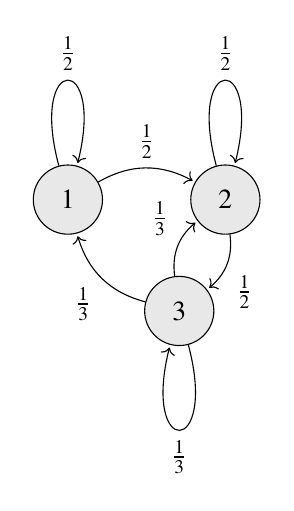
\begin{tikzpicture}[shorten >=1pt,node distance=2cm, scale =3, auto]
			\tikzstyle{every state}=[fill={rgb:black,1;white,10}]
			
			\node[state]   (q_1)                          {$1$};
			\node[state]   (q_2)  [right of=q_1]          {$2$};
			\node[state]   (q_3)  [below right of=q_1]          {$3$};
			
			\path[->]
			(q_1) edge [loop above] node {$\frac{1}{2}$}    (   )
			edge [bend left]  node {$\frac{1}{2}$}    (q_2)
			(q_2) edge [bend left]  node {$\frac{1}{2}$}    (q_3)
			edge [loop above] node {$\frac{1}{2}$}    ()
			(q_3) edge [bend left]  node {$\frac{1}{3}$}    (q_2)
			edge [bend left]  node {$\frac{1}{3}$}    (q_1)
			edge [loop below] node {$\frac{1}{3}$}    ();
		\end{tikzpicture}$
		
		\\  
		&\\
		&\\
		\hline
		\multirow{3}{*}{Checking whether the  } & \\
		& Here,\\chain is Irreducible
		& All the states are accessible to one another. \\and Aperiodic
		& $\implies$ They are in the same communication class. So, it is Irreducible.\\
		& \\
		& There exists the non- zero self-transition, which means that the chain \\
		& is Aperiodic.\\
		&\\ 
		& We know that if the Markov Chain is irreducible and aperiodic then \\
		& \qquad \qquad \qquad $\Vec{\pi}_{j} = \lim_{n \to \infty}P\{X_{n} = j\}$, $j = 1,...,N$ \\
		& These are the stationary probabilities. \\
		&\\
		\hline
		\multirow{3}{*}{Finding the Stationary} & \\
		& Stationary Probability can be represented as\\Probability Distributions
		& \qquad \qquad \qquad $\Vec{\pi} = \Vec{\pi} \vec{P}$\\
		& \\
		& \qquad $\implies$ $\myvec{v_{1}&&v_{2}&&v_{3}} = \myvec{v_{1}&&v_{2}&&v_{3}}\vec{P}$ \\
		& \\
		& Equating the above equation we get \\
		& \\
		& \qquad \qquad \qquad $\frac{1}{2}v_{1}-\frac{1}{3}v_{3} = 0$ $\label{eq:solutions/2018/dec/106/eq}$\\
		& \\
		& \qquad \qquad \qquad $\frac{1}{2}v_{1}-\frac{1}{2}v_{2} + \frac{1}{3}v_{3} = 0$\\
		& \\
		& \qquad \qquad \qquad $\frac{1}{2}v_{2}-\frac{2}{3}v_{3} = 0$\\
		& \\\
		& We see that summation of second and the third equation gives us the \\
		& first equation only. \\
		& And we know that the probability distribution will sum up to 1. \\
		& \\
		& \qquad \qquad \qquad $v_{1}+v_{2}+v_{3} = 1$ \\
		& \\
		& Therefore, we get the equation form as \\
		& \\
		& \qquad \qquad \qquad $\myvec{1&1&1\\\frac{1}{2}&0&\frac{-1}{3}\\\frac{1}{2}&\frac{-1}{2}&\frac{1}{3}}\myvec{v_{1}\\v_{2}\\v_{3}} = \myvec{1\\0\\0}$ \\
		& \\
		\hline
		\multirow{3}{*}{Solving the linear} & \\
		& The above linear equation can be solved using Gauss-Jordan method as\\equtions
		& \\
		& \qquad \qquad \qquad $\myvec{1&1&1&\vrule&1\\\frac{1}{2}&0&\frac{-1}{3}&\vrule&0\\\frac{1}{2}&\frac{-1}{2}&\frac{1}{3}&\vrule&0}$\\
		& \\
		& \qquad $\xleftrightarrow[]{R_2 \leftarrow R_2 - \frac{1}{2}R_1}$
		$\myvec{1&1&1&\vrule&1\\0&\frac{-1}{2}&\frac{-5}{6}&\vrule&\frac{-1}{2}\\\frac{1}{2}&\frac{-1}{2}&\frac{1}{3}&\vrule&0}$\\
		&\\
		& \qquad $\xleftrightarrow[]{R_3 \leftarrow R_3 - \frac{1}{2}R_1}$
		$\myvec{1&1&1&\vrule&1\\0&\frac{-1}{2}&\frac{-5}{6}&\vrule&\frac{-1}{2}\\0&-1&\frac{-1}{6}&\vrule&\frac{-1}{2}}$\\
		&\\
		& \qquad $\xleftrightarrow[]{R_2 \leftarrow \frac{-1}{2}R_2}$
		$\myvec{1&1&1&\vrule&1\\0&1&\frac{5}{3}&\vrule&1\\0&-1&\frac{-1}{6}&\vrule&\frac{-1}{2}}$\\
		&\\
		& \qquad $\xleftrightarrow[]{R_3 \leftarrow R_3 + R_2}$
		$\myvec{1&1&1&\vrule&1\\0&1&\frac{5}{3}&\vrule&1\\0&0&\frac{3}{2}&\vrule&\frac{1}{2}}$\\
		&\\
		& \qquad $\xleftrightarrow[]{R_3 \leftarrow \frac{3}{2}R_3}$
		$\myvec{1&1&1&\vrule&1\\0&1&\frac{5}{3}&\vrule&1\\0&0&1&\vrule&\frac{1}{3}}$\\
		&\\
		& \qquad $\xleftrightarrow[]{R_2 \leftarrow R_2 - \frac{5}{3}R_3}$
		$\myvec{1&1&1&\vrule&1\\0&1&0&\vrule&\frac{4}{9}\\0&0&1&\vrule&\frac{1}{3}}$\\
		&\\
		& \qquad $\xleftrightarrow[]{R_1 \leftarrow R_1 - R_3}$
		$\myvec{1&1&0&\vrule&\frac{2}{3}\\0&1&0&\vrule&\frac{4}{9}\\0&0&1&\vrule&\frac{1}{3}}$\\
		&\\
		& \qquad $\xleftrightarrow[]{R_1 \leftarrow R_1 - R_2}$
		$\myvec{1&0&0&\vrule&\frac{2}{9}\\0&1&0&\vrule&\frac{4}{9}\\0&0&1&\vrule&\frac{1}{3}}$\\
		&\\
		& $\therefore$, stationary probability distribution $\pi$ is given by \\
		& \qquad \qquad $\pi = \myvec{\frac{2}{9} & \frac{4}{9} & \frac{1}{3}}$ \\
		& \\
		\hline
		\multirow{3}{*}{Observations} & \\
		
		
		& Since the given transition probability matrix $\vec{P}$ is irreducible and aperiodic, \\
		& then $\lim_{n \to \infty} \vec{P}^{n}$ converges to a matrix with all rows identical and equal to $\vec{\pi}$. \\
		& \\
		& We were able to find $\vec{\pi}$ as $\myvec{\frac{2}{9} & \frac{4}{9} & \frac{1}{3}}$ \\
		& \\
		& $\lim_{n \to \infty} \vec{P}^{n} = \myvec{\frac{2}{9}&\frac{4}{9}&\frac{1}{3}\\\frac{2}{9}&\frac{4}{9}&\frac{1}{3}\\\frac{2}{9}&\frac{4}{9}&\frac{1}{3}}$\\
		& \\
		& From the above matrix, we get \\
		& \\
		& $\lim_{n \to \infty} \vec{P}^{n}_{11} = \frac{2}{9}$ \\
		&\\
		& $\lim_{n \to \infty} \vec{P}^{n}_{21} = \frac{2}{9}$ \\
		&\\
		& $\lim_{n \to \infty} \vec{P}^{n}_{32} = \frac{4}{9}$ \\
		&\\
		& $\lim_{n \to \infty} \vec{P}^{n}_{13} = \frac{1}{3}$ \\
		&\\
		\hline
		\multirow{3}{*}{Conclusion} & \\
		& From our observation we see that \\
		&\\
		& Options 1) and 4) are True.\\
		& \\
		\hline
\caption{}
\label{eq:solutions/2018/dec/106/table1}
	\end{longtable}
\twocolumn

\item Let
\begin{align}
\vec{M} = 
\myvec
{
2 & 0 & 3 & 2 & 0 & -2
\\
0 & 1 & 0 & -1 & 3 & 4
\\
0 & 0 & 1 & 0 & 4 & 4
\\
1 & 1 & 1 & 0 & 1 & 1
}
\\
\vec{b}_1 = \myvec{5 \\ 1 \\ 1 \\ 4},
\vec{b}_2 = \myvec{5 \\ 1 \\ 3 \\ 3}.
\end{align}  
Then which of the following are true?
\begin{enumerate}
\item both systems $\vec{M}\vec{x} = \vec{b}_1$ and $\vec{M}\vec{x} = \vec{b}_2$ are inconsistent.
\item both systems $\vec{M}\vec{x} = \vec{b}_1$ and $\vec{M}\vec{x} = \vec{b}_2$ are consistent. 
\item the system $\vec{M}\vec{x} = \vec{b}_1-\vec{b}_2$ is consistent. 
\item the system $\vec{M}\vec{x} = \vec{b}_1-\vec{b}_2$ is inconsistent. 
\end{enumerate}
%
%
\solution
See Tables \ref{eq:solutions/2018/dec/106/table0} and \ref{eq:solutions/2018/dec/106/table1}


\onecolumn
	\begin{longtable}{|l|l|}
		\hline
		\multirow{3}{*}{Irreducible Markov Chain} 
		& \\
		& A Markov chain is $\textbf{irreducible}$ if all the states communicate with each other,\\
		& i.e., if there is only one communication class.\\
		&\\
		\hline
		\multirow{3}{*}{Aperiodic Markov Chain} & \\
		& If there is a self-transition in the chain ($p^{ii}>0$ for some i), then the chain is\\
		& called as $\textbf{aperiodic}$\\
		& \\
		\hline
		\multirow{3}{*}{Stationary Distribution} & \\
		& A stationary distribution of a Markov chain is a probability distribution that\\
		& remains unchanged in the Markov chain as time progresses. Typically, it is\\
		& represented as a row vector $\Vec{\pi}$ whose entries are probabilities summing to 1,\\ 
		& and given transition matrix $\textbf{P}$, it satisfies\\
		& \\
		&  \qquad \qquad  \qquad$\Vec{\pi} = \Vec{\pi} \textbf{P}$\\
		& \\
		\hline
\caption{}
\label{eq:solutions/2018/dec/106/table0}
	\end{longtable}
	\begin{longtable}{|l|l|}
		\hline
		\multirow{3}{*}{Drawing Transition diagram} 
		& \\
		& 
		
		$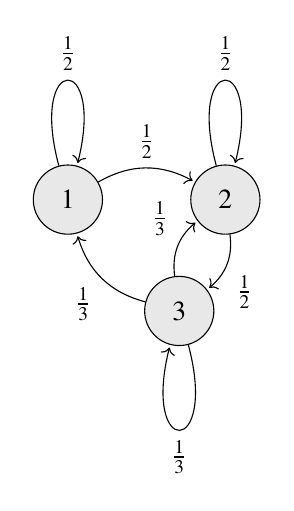
\begin{tikzpicture}[shorten >=1pt,node distance=2cm, scale =3, auto]
			\tikzstyle{every state}=[fill={rgb:black,1;white,10}]
			
			\node[state]   (q_1)                          {$1$};
			\node[state]   (q_2)  [right of=q_1]          {$2$};
			\node[state]   (q_3)  [below right of=q_1]          {$3$};
			
			\path[->]
			(q_1) edge [loop above] node {$\frac{1}{2}$}    (   )
			edge [bend left]  node {$\frac{1}{2}$}    (q_2)
			(q_2) edge [bend left]  node {$\frac{1}{2}$}    (q_3)
			edge [loop above] node {$\frac{1}{2}$}    ()
			(q_3) edge [bend left]  node {$\frac{1}{3}$}    (q_2)
			edge [bend left]  node {$\frac{1}{3}$}    (q_1)
			edge [loop below] node {$\frac{1}{3}$}    ();
		\end{tikzpicture}$
		
		\\  
		&\\
		&\\
		\hline
		\multirow{3}{*}{Checking whether the  } & \\
		& Here,\\chain is Irreducible
		& All the states are accessible to one another. \\and Aperiodic
		& $\implies$ They are in the same communication class. So, it is Irreducible.\\
		& \\
		& There exists the non- zero self-transition, which means that the chain \\
		& is Aperiodic.\\
		&\\ 
		& We know that if the Markov Chain is irreducible and aperiodic then \\
		& \qquad \qquad \qquad $\Vec{\pi}_{j} = \lim_{n \to \infty}P\{X_{n} = j\}$, $j = 1,...,N$ \\
		& These are the stationary probabilities. \\
		&\\
		\hline
		\multirow{3}{*}{Finding the Stationary} & \\
		& Stationary Probability can be represented as\\Probability Distributions
		& \qquad \qquad \qquad $\Vec{\pi} = \Vec{\pi} \vec{P}$\\
		& \\
		& \qquad $\implies$ $\myvec{v_{1}&&v_{2}&&v_{3}} = \myvec{v_{1}&&v_{2}&&v_{3}}\vec{P}$ \\
		& \\
		& Equating the above equation we get \\
		& \\
		& \qquad \qquad \qquad $\frac{1}{2}v_{1}-\frac{1}{3}v_{3} = 0$ $\label{eq:solutions/2018/dec/106/eq}$\\
		& \\
		& \qquad \qquad \qquad $\frac{1}{2}v_{1}-\frac{1}{2}v_{2} + \frac{1}{3}v_{3} = 0$\\
		& \\
		& \qquad \qquad \qquad $\frac{1}{2}v_{2}-\frac{2}{3}v_{3} = 0$\\
		& \\\
		& We see that summation of second and the third equation gives us the \\
		& first equation only. \\
		& And we know that the probability distribution will sum up to 1. \\
		& \\
		& \qquad \qquad \qquad $v_{1}+v_{2}+v_{3} = 1$ \\
		& \\
		& Therefore, we get the equation form as \\
		& \\
		& \qquad \qquad \qquad $\myvec{1&1&1\\\frac{1}{2}&0&\frac{-1}{3}\\\frac{1}{2}&\frac{-1}{2}&\frac{1}{3}}\myvec{v_{1}\\v_{2}\\v_{3}} = \myvec{1\\0\\0}$ \\
		& \\
		\hline
		\multirow{3}{*}{Solving the linear} & \\
		& The above linear equation can be solved using Gauss-Jordan method as\\equtions
		& \\
		& \qquad \qquad \qquad $\myvec{1&1&1&\vrule&1\\\frac{1}{2}&0&\frac{-1}{3}&\vrule&0\\\frac{1}{2}&\frac{-1}{2}&\frac{1}{3}&\vrule&0}$\\
		& \\
		& \qquad $\xleftrightarrow[]{R_2 \leftarrow R_2 - \frac{1}{2}R_1}$
		$\myvec{1&1&1&\vrule&1\\0&\frac{-1}{2}&\frac{-5}{6}&\vrule&\frac{-1}{2}\\\frac{1}{2}&\frac{-1}{2}&\frac{1}{3}&\vrule&0}$\\
		&\\
		& \qquad $\xleftrightarrow[]{R_3 \leftarrow R_3 - \frac{1}{2}R_1}$
		$\myvec{1&1&1&\vrule&1\\0&\frac{-1}{2}&\frac{-5}{6}&\vrule&\frac{-1}{2}\\0&-1&\frac{-1}{6}&\vrule&\frac{-1}{2}}$\\
		&\\
		& \qquad $\xleftrightarrow[]{R_2 \leftarrow \frac{-1}{2}R_2}$
		$\myvec{1&1&1&\vrule&1\\0&1&\frac{5}{3}&\vrule&1\\0&-1&\frac{-1}{6}&\vrule&\frac{-1}{2}}$\\
		&\\
		& \qquad $\xleftrightarrow[]{R_3 \leftarrow R_3 + R_2}$
		$\myvec{1&1&1&\vrule&1\\0&1&\frac{5}{3}&\vrule&1\\0&0&\frac{3}{2}&\vrule&\frac{1}{2}}$\\
		&\\
		& \qquad $\xleftrightarrow[]{R_3 \leftarrow \frac{3}{2}R_3}$
		$\myvec{1&1&1&\vrule&1\\0&1&\frac{5}{3}&\vrule&1\\0&0&1&\vrule&\frac{1}{3}}$\\
		&\\
		& \qquad $\xleftrightarrow[]{R_2 \leftarrow R_2 - \frac{5}{3}R_3}$
		$\myvec{1&1&1&\vrule&1\\0&1&0&\vrule&\frac{4}{9}\\0&0&1&\vrule&\frac{1}{3}}$\\
		&\\
		& \qquad $\xleftrightarrow[]{R_1 \leftarrow R_1 - R_3}$
		$\myvec{1&1&0&\vrule&\frac{2}{3}\\0&1&0&\vrule&\frac{4}{9}\\0&0&1&\vrule&\frac{1}{3}}$\\
		&\\
		& \qquad $\xleftrightarrow[]{R_1 \leftarrow R_1 - R_2}$
		$\myvec{1&0&0&\vrule&\frac{2}{9}\\0&1&0&\vrule&\frac{4}{9}\\0&0&1&\vrule&\frac{1}{3}}$\\
		&\\
		& $\therefore$, stationary probability distribution $\pi$ is given by \\
		& \qquad \qquad $\pi = \myvec{\frac{2}{9} & \frac{4}{9} & \frac{1}{3}}$ \\
		& \\
		\hline
		\multirow{3}{*}{Observations} & \\
		
		
		& Since the given transition probability matrix $\vec{P}$ is irreducible and aperiodic, \\
		& then $\lim_{n \to \infty} \vec{P}^{n}$ converges to a matrix with all rows identical and equal to $\vec{\pi}$. \\
		& \\
		& We were able to find $\vec{\pi}$ as $\myvec{\frac{2}{9} & \frac{4}{9} & \frac{1}{3}}$ \\
		& \\
		& $\lim_{n \to \infty} \vec{P}^{n} = \myvec{\frac{2}{9}&\frac{4}{9}&\frac{1}{3}\\\frac{2}{9}&\frac{4}{9}&\frac{1}{3}\\\frac{2}{9}&\frac{4}{9}&\frac{1}{3}}$\\
		& \\
		& From the above matrix, we get \\
		& \\
		& $\lim_{n \to \infty} \vec{P}^{n}_{11} = \frac{2}{9}$ \\
		&\\
		& $\lim_{n \to \infty} \vec{P}^{n}_{21} = \frac{2}{9}$ \\
		&\\
		& $\lim_{n \to \infty} \vec{P}^{n}_{32} = \frac{4}{9}$ \\
		&\\
		& $\lim_{n \to \infty} \vec{P}^{n}_{13} = \frac{1}{3}$ \\
		&\\
		\hline
		\multirow{3}{*}{Conclusion} & \\
		& From our observation we see that \\
		&\\
		& Options 1) and 4) are True.\\
		& \\
		\hline
\caption{}
\label{eq:solutions/2018/dec/106/table1}
	\end{longtable}
\twocolumn

\item Let 
\begin{align}
\vec{M} = \myvec
{
1 & -1 & 1 \\
2 & 1 & 4 \\
-2 & 1 & -4 
}.
\end{align}
Given that 1 is an eigenvalue of $\vec{M}$, then which among the following
are correct?
\begin{enumerate}
\item The minimal polynomial of  $\vec{M}$ is $\brak{x-1}\brak{x+4}$ 
\item The minimal polynomial of  $\vec{M}$ is $\brak{x-1}^2\brak{x+4}$ 
\item   $\vec{M}$ is not diagonalizable.
\item $\vec{M}^{-1} = \frac{1}{4}\brak{\vec{M}+3\vec{I}}$. 
\end{enumerate}
%
\solution
See Tables \ref{eq:solutions/2018/dec/106/table0} and \ref{eq:solutions/2018/dec/106/table1}


\onecolumn
	\begin{longtable}{|l|l|}
		\hline
		\multirow{3}{*}{Irreducible Markov Chain} 
		& \\
		& A Markov chain is $\textbf{irreducible}$ if all the states communicate with each other,\\
		& i.e., if there is only one communication class.\\
		&\\
		\hline
		\multirow{3}{*}{Aperiodic Markov Chain} & \\
		& If there is a self-transition in the chain ($p^{ii}>0$ for some i), then the chain is\\
		& called as $\textbf{aperiodic}$\\
		& \\
		\hline
		\multirow{3}{*}{Stationary Distribution} & \\
		& A stationary distribution of a Markov chain is a probability distribution that\\
		& remains unchanged in the Markov chain as time progresses. Typically, it is\\
		& represented as a row vector $\Vec{\pi}$ whose entries are probabilities summing to 1,\\ 
		& and given transition matrix $\textbf{P}$, it satisfies\\
		& \\
		&  \qquad \qquad  \qquad$\Vec{\pi} = \Vec{\pi} \textbf{P}$\\
		& \\
		\hline
\caption{}
\label{eq:solutions/2018/dec/106/table0}
	\end{longtable}
	\begin{longtable}{|l|l|}
		\hline
		\multirow{3}{*}{Drawing Transition diagram} 
		& \\
		& 
		
		$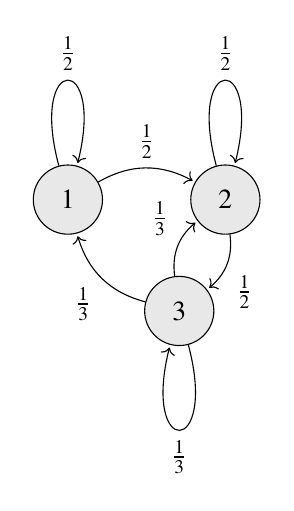
\begin{tikzpicture}[shorten >=1pt,node distance=2cm, scale =3, auto]
			\tikzstyle{every state}=[fill={rgb:black,1;white,10}]
			
			\node[state]   (q_1)                          {$1$};
			\node[state]   (q_2)  [right of=q_1]          {$2$};
			\node[state]   (q_3)  [below right of=q_1]          {$3$};
			
			\path[->]
			(q_1) edge [loop above] node {$\frac{1}{2}$}    (   )
			edge [bend left]  node {$\frac{1}{2}$}    (q_2)
			(q_2) edge [bend left]  node {$\frac{1}{2}$}    (q_3)
			edge [loop above] node {$\frac{1}{2}$}    ()
			(q_3) edge [bend left]  node {$\frac{1}{3}$}    (q_2)
			edge [bend left]  node {$\frac{1}{3}$}    (q_1)
			edge [loop below] node {$\frac{1}{3}$}    ();
		\end{tikzpicture}$
		
		\\  
		&\\
		&\\
		\hline
		\multirow{3}{*}{Checking whether the  } & \\
		& Here,\\chain is Irreducible
		& All the states are accessible to one another. \\and Aperiodic
		& $\implies$ They are in the same communication class. So, it is Irreducible.\\
		& \\
		& There exists the non- zero self-transition, which means that the chain \\
		& is Aperiodic.\\
		&\\ 
		& We know that if the Markov Chain is irreducible and aperiodic then \\
		& \qquad \qquad \qquad $\Vec{\pi}_{j} = \lim_{n \to \infty}P\{X_{n} = j\}$, $j = 1,...,N$ \\
		& These are the stationary probabilities. \\
		&\\
		\hline
		\multirow{3}{*}{Finding the Stationary} & \\
		& Stationary Probability can be represented as\\Probability Distributions
		& \qquad \qquad \qquad $\Vec{\pi} = \Vec{\pi} \vec{P}$\\
		& \\
		& \qquad $\implies$ $\myvec{v_{1}&&v_{2}&&v_{3}} = \myvec{v_{1}&&v_{2}&&v_{3}}\vec{P}$ \\
		& \\
		& Equating the above equation we get \\
		& \\
		& \qquad \qquad \qquad $\frac{1}{2}v_{1}-\frac{1}{3}v_{3} = 0$ $\label{eq:solutions/2018/dec/106/eq}$\\
		& \\
		& \qquad \qquad \qquad $\frac{1}{2}v_{1}-\frac{1}{2}v_{2} + \frac{1}{3}v_{3} = 0$\\
		& \\
		& \qquad \qquad \qquad $\frac{1}{2}v_{2}-\frac{2}{3}v_{3} = 0$\\
		& \\\
		& We see that summation of second and the third equation gives us the \\
		& first equation only. \\
		& And we know that the probability distribution will sum up to 1. \\
		& \\
		& \qquad \qquad \qquad $v_{1}+v_{2}+v_{3} = 1$ \\
		& \\
		& Therefore, we get the equation form as \\
		& \\
		& \qquad \qquad \qquad $\myvec{1&1&1\\\frac{1}{2}&0&\frac{-1}{3}\\\frac{1}{2}&\frac{-1}{2}&\frac{1}{3}}\myvec{v_{1}\\v_{2}\\v_{3}} = \myvec{1\\0\\0}$ \\
		& \\
		\hline
		\multirow{3}{*}{Solving the linear} & \\
		& The above linear equation can be solved using Gauss-Jordan method as\\equtions
		& \\
		& \qquad \qquad \qquad $\myvec{1&1&1&\vrule&1\\\frac{1}{2}&0&\frac{-1}{3}&\vrule&0\\\frac{1}{2}&\frac{-1}{2}&\frac{1}{3}&\vrule&0}$\\
		& \\
		& \qquad $\xleftrightarrow[]{R_2 \leftarrow R_2 - \frac{1}{2}R_1}$
		$\myvec{1&1&1&\vrule&1\\0&\frac{-1}{2}&\frac{-5}{6}&\vrule&\frac{-1}{2}\\\frac{1}{2}&\frac{-1}{2}&\frac{1}{3}&\vrule&0}$\\
		&\\
		& \qquad $\xleftrightarrow[]{R_3 \leftarrow R_3 - \frac{1}{2}R_1}$
		$\myvec{1&1&1&\vrule&1\\0&\frac{-1}{2}&\frac{-5}{6}&\vrule&\frac{-1}{2}\\0&-1&\frac{-1}{6}&\vrule&\frac{-1}{2}}$\\
		&\\
		& \qquad $\xleftrightarrow[]{R_2 \leftarrow \frac{-1}{2}R_2}$
		$\myvec{1&1&1&\vrule&1\\0&1&\frac{5}{3}&\vrule&1\\0&-1&\frac{-1}{6}&\vrule&\frac{-1}{2}}$\\
		&\\
		& \qquad $\xleftrightarrow[]{R_3 \leftarrow R_3 + R_2}$
		$\myvec{1&1&1&\vrule&1\\0&1&\frac{5}{3}&\vrule&1\\0&0&\frac{3}{2}&\vrule&\frac{1}{2}}$\\
		&\\
		& \qquad $\xleftrightarrow[]{R_3 \leftarrow \frac{3}{2}R_3}$
		$\myvec{1&1&1&\vrule&1\\0&1&\frac{5}{3}&\vrule&1\\0&0&1&\vrule&\frac{1}{3}}$\\
		&\\
		& \qquad $\xleftrightarrow[]{R_2 \leftarrow R_2 - \frac{5}{3}R_3}$
		$\myvec{1&1&1&\vrule&1\\0&1&0&\vrule&\frac{4}{9}\\0&0&1&\vrule&\frac{1}{3}}$\\
		&\\
		& \qquad $\xleftrightarrow[]{R_1 \leftarrow R_1 - R_3}$
		$\myvec{1&1&0&\vrule&\frac{2}{3}\\0&1&0&\vrule&\frac{4}{9}\\0&0&1&\vrule&\frac{1}{3}}$\\
		&\\
		& \qquad $\xleftrightarrow[]{R_1 \leftarrow R_1 - R_2}$
		$\myvec{1&0&0&\vrule&\frac{2}{9}\\0&1&0&\vrule&\frac{4}{9}\\0&0&1&\vrule&\frac{1}{3}}$\\
		&\\
		& $\therefore$, stationary probability distribution $\pi$ is given by \\
		& \qquad \qquad $\pi = \myvec{\frac{2}{9} & \frac{4}{9} & \frac{1}{3}}$ \\
		& \\
		\hline
		\multirow{3}{*}{Observations} & \\
		
		
		& Since the given transition probability matrix $\vec{P}$ is irreducible and aperiodic, \\
		& then $\lim_{n \to \infty} \vec{P}^{n}$ converges to a matrix with all rows identical and equal to $\vec{\pi}$. \\
		& \\
		& We were able to find $\vec{\pi}$ as $\myvec{\frac{2}{9} & \frac{4}{9} & \frac{1}{3}}$ \\
		& \\
		& $\lim_{n \to \infty} \vec{P}^{n} = \myvec{\frac{2}{9}&\frac{4}{9}&\frac{1}{3}\\\frac{2}{9}&\frac{4}{9}&\frac{1}{3}\\\frac{2}{9}&\frac{4}{9}&\frac{1}{3}}$\\
		& \\
		& From the above matrix, we get \\
		& \\
		& $\lim_{n \to \infty} \vec{P}^{n}_{11} = \frac{2}{9}$ \\
		&\\
		& $\lim_{n \to \infty} \vec{P}^{n}_{21} = \frac{2}{9}$ \\
		&\\
		& $\lim_{n \to \infty} \vec{P}^{n}_{32} = \frac{4}{9}$ \\
		&\\
		& $\lim_{n \to \infty} \vec{P}^{n}_{13} = \frac{1}{3}$ \\
		&\\
		\hline
		\multirow{3}{*}{Conclusion} & \\
		& From our observation we see that \\
		&\\
		& Options 1) and 4) are True.\\
		& \\
		\hline
\caption{}
\label{eq:solutions/2018/dec/106/table1}
	\end{longtable}
\twocolumn

\item Let $\vec{A}$ be a real matrix with characteristic polynomial $\brak{x-1}^3$.  Pick the correct statements from below:
\begin{enumerate}
\item $\vec{A}$ is necessarily diagonalizable.
\item If the minimal polynomial of  $\vec{A}$ is $\brak{x-1}^3$, then  $\vec{A}$ is diagonalizable.
\item  The characteristic polynomial of  $\vec{A}^2$ is $\brak{x-1}^3$
\item If $\vec{A}$ has exactly two Jordan blocks, then $\brak{\vec{A}-\vec{I}}^2$ is diagonalizable. 
\end{enumerate}
\solution
See Tables \ref{eq:solutions/2018/dec/106/table0} and \ref{eq:solutions/2018/dec/106/table1}


\onecolumn
	\begin{longtable}{|l|l|}
		\hline
		\multirow{3}{*}{Irreducible Markov Chain} 
		& \\
		& A Markov chain is $\textbf{irreducible}$ if all the states communicate with each other,\\
		& i.e., if there is only one communication class.\\
		&\\
		\hline
		\multirow{3}{*}{Aperiodic Markov Chain} & \\
		& If there is a self-transition in the chain ($p^{ii}>0$ for some i), then the chain is\\
		& called as $\textbf{aperiodic}$\\
		& \\
		\hline
		\multirow{3}{*}{Stationary Distribution} & \\
		& A stationary distribution of a Markov chain is a probability distribution that\\
		& remains unchanged in the Markov chain as time progresses. Typically, it is\\
		& represented as a row vector $\Vec{\pi}$ whose entries are probabilities summing to 1,\\ 
		& and given transition matrix $\textbf{P}$, it satisfies\\
		& \\
		&  \qquad \qquad  \qquad$\Vec{\pi} = \Vec{\pi} \textbf{P}$\\
		& \\
		\hline
\caption{}
\label{eq:solutions/2018/dec/106/table0}
	\end{longtable}
	\begin{longtable}{|l|l|}
		\hline
		\multirow{3}{*}{Drawing Transition diagram} 
		& \\
		& 
		
		$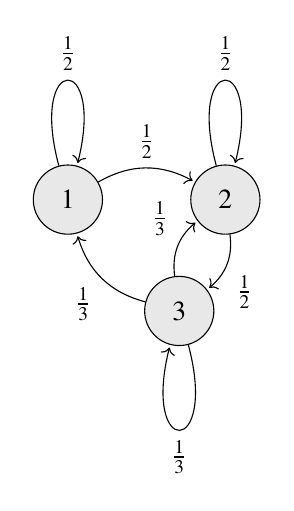
\begin{tikzpicture}[shorten >=1pt,node distance=2cm, scale =3, auto]
			\tikzstyle{every state}=[fill={rgb:black,1;white,10}]
			
			\node[state]   (q_1)                          {$1$};
			\node[state]   (q_2)  [right of=q_1]          {$2$};
			\node[state]   (q_3)  [below right of=q_1]          {$3$};
			
			\path[->]
			(q_1) edge [loop above] node {$\frac{1}{2}$}    (   )
			edge [bend left]  node {$\frac{1}{2}$}    (q_2)
			(q_2) edge [bend left]  node {$\frac{1}{2}$}    (q_3)
			edge [loop above] node {$\frac{1}{2}$}    ()
			(q_3) edge [bend left]  node {$\frac{1}{3}$}    (q_2)
			edge [bend left]  node {$\frac{1}{3}$}    (q_1)
			edge [loop below] node {$\frac{1}{3}$}    ();
		\end{tikzpicture}$
		
		\\  
		&\\
		&\\
		\hline
		\multirow{3}{*}{Checking whether the  } & \\
		& Here,\\chain is Irreducible
		& All the states are accessible to one another. \\and Aperiodic
		& $\implies$ They are in the same communication class. So, it is Irreducible.\\
		& \\
		& There exists the non- zero self-transition, which means that the chain \\
		& is Aperiodic.\\
		&\\ 
		& We know that if the Markov Chain is irreducible and aperiodic then \\
		& \qquad \qquad \qquad $\Vec{\pi}_{j} = \lim_{n \to \infty}P\{X_{n} = j\}$, $j = 1,...,N$ \\
		& These are the stationary probabilities. \\
		&\\
		\hline
		\multirow{3}{*}{Finding the Stationary} & \\
		& Stationary Probability can be represented as\\Probability Distributions
		& \qquad \qquad \qquad $\Vec{\pi} = \Vec{\pi} \vec{P}$\\
		& \\
		& \qquad $\implies$ $\myvec{v_{1}&&v_{2}&&v_{3}} = \myvec{v_{1}&&v_{2}&&v_{3}}\vec{P}$ \\
		& \\
		& Equating the above equation we get \\
		& \\
		& \qquad \qquad \qquad $\frac{1}{2}v_{1}-\frac{1}{3}v_{3} = 0$ $\label{eq:solutions/2018/dec/106/eq}$\\
		& \\
		& \qquad \qquad \qquad $\frac{1}{2}v_{1}-\frac{1}{2}v_{2} + \frac{1}{3}v_{3} = 0$\\
		& \\
		& \qquad \qquad \qquad $\frac{1}{2}v_{2}-\frac{2}{3}v_{3} = 0$\\
		& \\\
		& We see that summation of second and the third equation gives us the \\
		& first equation only. \\
		& And we know that the probability distribution will sum up to 1. \\
		& \\
		& \qquad \qquad \qquad $v_{1}+v_{2}+v_{3} = 1$ \\
		& \\
		& Therefore, we get the equation form as \\
		& \\
		& \qquad \qquad \qquad $\myvec{1&1&1\\\frac{1}{2}&0&\frac{-1}{3}\\\frac{1}{2}&\frac{-1}{2}&\frac{1}{3}}\myvec{v_{1}\\v_{2}\\v_{3}} = \myvec{1\\0\\0}$ \\
		& \\
		\hline
		\multirow{3}{*}{Solving the linear} & \\
		& The above linear equation can be solved using Gauss-Jordan method as\\equtions
		& \\
		& \qquad \qquad \qquad $\myvec{1&1&1&\vrule&1\\\frac{1}{2}&0&\frac{-1}{3}&\vrule&0\\\frac{1}{2}&\frac{-1}{2}&\frac{1}{3}&\vrule&0}$\\
		& \\
		& \qquad $\xleftrightarrow[]{R_2 \leftarrow R_2 - \frac{1}{2}R_1}$
		$\myvec{1&1&1&\vrule&1\\0&\frac{-1}{2}&\frac{-5}{6}&\vrule&\frac{-1}{2}\\\frac{1}{2}&\frac{-1}{2}&\frac{1}{3}&\vrule&0}$\\
		&\\
		& \qquad $\xleftrightarrow[]{R_3 \leftarrow R_3 - \frac{1}{2}R_1}$
		$\myvec{1&1&1&\vrule&1\\0&\frac{-1}{2}&\frac{-5}{6}&\vrule&\frac{-1}{2}\\0&-1&\frac{-1}{6}&\vrule&\frac{-1}{2}}$\\
		&\\
		& \qquad $\xleftrightarrow[]{R_2 \leftarrow \frac{-1}{2}R_2}$
		$\myvec{1&1&1&\vrule&1\\0&1&\frac{5}{3}&\vrule&1\\0&-1&\frac{-1}{6}&\vrule&\frac{-1}{2}}$\\
		&\\
		& \qquad $\xleftrightarrow[]{R_3 \leftarrow R_3 + R_2}$
		$\myvec{1&1&1&\vrule&1\\0&1&\frac{5}{3}&\vrule&1\\0&0&\frac{3}{2}&\vrule&\frac{1}{2}}$\\
		&\\
		& \qquad $\xleftrightarrow[]{R_3 \leftarrow \frac{3}{2}R_3}$
		$\myvec{1&1&1&\vrule&1\\0&1&\frac{5}{3}&\vrule&1\\0&0&1&\vrule&\frac{1}{3}}$\\
		&\\
		& \qquad $\xleftrightarrow[]{R_2 \leftarrow R_2 - \frac{5}{3}R_3}$
		$\myvec{1&1&1&\vrule&1\\0&1&0&\vrule&\frac{4}{9}\\0&0&1&\vrule&\frac{1}{3}}$\\
		&\\
		& \qquad $\xleftrightarrow[]{R_1 \leftarrow R_1 - R_3}$
		$\myvec{1&1&0&\vrule&\frac{2}{3}\\0&1&0&\vrule&\frac{4}{9}\\0&0&1&\vrule&\frac{1}{3}}$\\
		&\\
		& \qquad $\xleftrightarrow[]{R_1 \leftarrow R_1 - R_2}$
		$\myvec{1&0&0&\vrule&\frac{2}{9}\\0&1&0&\vrule&\frac{4}{9}\\0&0&1&\vrule&\frac{1}{3}}$\\
		&\\
		& $\therefore$, stationary probability distribution $\pi$ is given by \\
		& \qquad \qquad $\pi = \myvec{\frac{2}{9} & \frac{4}{9} & \frac{1}{3}}$ \\
		& \\
		\hline
		\multirow{3}{*}{Observations} & \\
		
		
		& Since the given transition probability matrix $\vec{P}$ is irreducible and aperiodic, \\
		& then $\lim_{n \to \infty} \vec{P}^{n}$ converges to a matrix with all rows identical and equal to $\vec{\pi}$. \\
		& \\
		& We were able to find $\vec{\pi}$ as $\myvec{\frac{2}{9} & \frac{4}{9} & \frac{1}{3}}$ \\
		& \\
		& $\lim_{n \to \infty} \vec{P}^{n} = \myvec{\frac{2}{9}&\frac{4}{9}&\frac{1}{3}\\\frac{2}{9}&\frac{4}{9}&\frac{1}{3}\\\frac{2}{9}&\frac{4}{9}&\frac{1}{3}}$\\
		& \\
		& From the above matrix, we get \\
		& \\
		& $\lim_{n \to \infty} \vec{P}^{n}_{11} = \frac{2}{9}$ \\
		&\\
		& $\lim_{n \to \infty} \vec{P}^{n}_{21} = \frac{2}{9}$ \\
		&\\
		& $\lim_{n \to \infty} \vec{P}^{n}_{32} = \frac{4}{9}$ \\
		&\\
		& $\lim_{n \to \infty} \vec{P}^{n}_{13} = \frac{1}{3}$ \\
		&\\
		\hline
		\multirow{3}{*}{Conclusion} & \\
		& From our observation we see that \\
		&\\
		& Options 1) and 4) are True.\\
		& \\
		\hline
\caption{}
\label{eq:solutions/2018/dec/106/table1}
	\end{longtable}
\twocolumn

%
\item Let $P_3$ be the vector space of polynomails with real coefficients and of degree at most 3.  Consider the linear map
\begin{align}
T:P_3\to P_3
\end{align}
defined by 
\begin{align}
T\brak{p(x)} = p(x-1)+p(x+1)
\end{align}
%
Which of the following properties does the matrix of $T$ with respect to the standard basis
$B = \cbrak{1,x,x^2,x^3}$ of $P_3$ satisfy?
\begin{enumerate}
\item $det T = 0$.
\item $\brak{T-2I}^4 = 0$ but $\brak{T-2I}^3 \ne 0$.
\item $\brak{T-2I}^3 = 0$ but $\brak{T-2I}^2 \ne 0$.
\item 2 is an eigenvalue with multiplicity 4.
\end{enumerate}
%
\solution
See Tables \ref{eq:solutions/2018/dec/106/table0} and \ref{eq:solutions/2018/dec/106/table1}


\onecolumn
	\begin{longtable}{|l|l|}
		\hline
		\multirow{3}{*}{Irreducible Markov Chain} 
		& \\
		& A Markov chain is $\textbf{irreducible}$ if all the states communicate with each other,\\
		& i.e., if there is only one communication class.\\
		&\\
		\hline
		\multirow{3}{*}{Aperiodic Markov Chain} & \\
		& If there is a self-transition in the chain ($p^{ii}>0$ for some i), then the chain is\\
		& called as $\textbf{aperiodic}$\\
		& \\
		\hline
		\multirow{3}{*}{Stationary Distribution} & \\
		& A stationary distribution of a Markov chain is a probability distribution that\\
		& remains unchanged in the Markov chain as time progresses. Typically, it is\\
		& represented as a row vector $\Vec{\pi}$ whose entries are probabilities summing to 1,\\ 
		& and given transition matrix $\textbf{P}$, it satisfies\\
		& \\
		&  \qquad \qquad  \qquad$\Vec{\pi} = \Vec{\pi} \textbf{P}$\\
		& \\
		\hline
\caption{}
\label{eq:solutions/2018/dec/106/table0}
	\end{longtable}
	\begin{longtable}{|l|l|}
		\hline
		\multirow{3}{*}{Drawing Transition diagram} 
		& \\
		& 
		
		$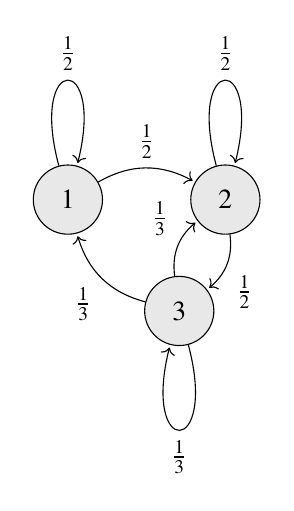
\begin{tikzpicture}[shorten >=1pt,node distance=2cm, scale =3, auto]
			\tikzstyle{every state}=[fill={rgb:black,1;white,10}]
			
			\node[state]   (q_1)                          {$1$};
			\node[state]   (q_2)  [right of=q_1]          {$2$};
			\node[state]   (q_3)  [below right of=q_1]          {$3$};
			
			\path[->]
			(q_1) edge [loop above] node {$\frac{1}{2}$}    (   )
			edge [bend left]  node {$\frac{1}{2}$}    (q_2)
			(q_2) edge [bend left]  node {$\frac{1}{2}$}    (q_3)
			edge [loop above] node {$\frac{1}{2}$}    ()
			(q_3) edge [bend left]  node {$\frac{1}{3}$}    (q_2)
			edge [bend left]  node {$\frac{1}{3}$}    (q_1)
			edge [loop below] node {$\frac{1}{3}$}    ();
		\end{tikzpicture}$
		
		\\  
		&\\
		&\\
		\hline
		\multirow{3}{*}{Checking whether the  } & \\
		& Here,\\chain is Irreducible
		& All the states are accessible to one another. \\and Aperiodic
		& $\implies$ They are in the same communication class. So, it is Irreducible.\\
		& \\
		& There exists the non- zero self-transition, which means that the chain \\
		& is Aperiodic.\\
		&\\ 
		& We know that if the Markov Chain is irreducible and aperiodic then \\
		& \qquad \qquad \qquad $\Vec{\pi}_{j} = \lim_{n \to \infty}P\{X_{n} = j\}$, $j = 1,...,N$ \\
		& These are the stationary probabilities. \\
		&\\
		\hline
		\multirow{3}{*}{Finding the Stationary} & \\
		& Stationary Probability can be represented as\\Probability Distributions
		& \qquad \qquad \qquad $\Vec{\pi} = \Vec{\pi} \vec{P}$\\
		& \\
		& \qquad $\implies$ $\myvec{v_{1}&&v_{2}&&v_{3}} = \myvec{v_{1}&&v_{2}&&v_{3}}\vec{P}$ \\
		& \\
		& Equating the above equation we get \\
		& \\
		& \qquad \qquad \qquad $\frac{1}{2}v_{1}-\frac{1}{3}v_{3} = 0$ $\label{eq:solutions/2018/dec/106/eq}$\\
		& \\
		& \qquad \qquad \qquad $\frac{1}{2}v_{1}-\frac{1}{2}v_{2} + \frac{1}{3}v_{3} = 0$\\
		& \\
		& \qquad \qquad \qquad $\frac{1}{2}v_{2}-\frac{2}{3}v_{3} = 0$\\
		& \\\
		& We see that summation of second and the third equation gives us the \\
		& first equation only. \\
		& And we know that the probability distribution will sum up to 1. \\
		& \\
		& \qquad \qquad \qquad $v_{1}+v_{2}+v_{3} = 1$ \\
		& \\
		& Therefore, we get the equation form as \\
		& \\
		& \qquad \qquad \qquad $\myvec{1&1&1\\\frac{1}{2}&0&\frac{-1}{3}\\\frac{1}{2}&\frac{-1}{2}&\frac{1}{3}}\myvec{v_{1}\\v_{2}\\v_{3}} = \myvec{1\\0\\0}$ \\
		& \\
		\hline
		\multirow{3}{*}{Solving the linear} & \\
		& The above linear equation can be solved using Gauss-Jordan method as\\equtions
		& \\
		& \qquad \qquad \qquad $\myvec{1&1&1&\vrule&1\\\frac{1}{2}&0&\frac{-1}{3}&\vrule&0\\\frac{1}{2}&\frac{-1}{2}&\frac{1}{3}&\vrule&0}$\\
		& \\
		& \qquad $\xleftrightarrow[]{R_2 \leftarrow R_2 - \frac{1}{2}R_1}$
		$\myvec{1&1&1&\vrule&1\\0&\frac{-1}{2}&\frac{-5}{6}&\vrule&\frac{-1}{2}\\\frac{1}{2}&\frac{-1}{2}&\frac{1}{3}&\vrule&0}$\\
		&\\
		& \qquad $\xleftrightarrow[]{R_3 \leftarrow R_3 - \frac{1}{2}R_1}$
		$\myvec{1&1&1&\vrule&1\\0&\frac{-1}{2}&\frac{-5}{6}&\vrule&\frac{-1}{2}\\0&-1&\frac{-1}{6}&\vrule&\frac{-1}{2}}$\\
		&\\
		& \qquad $\xleftrightarrow[]{R_2 \leftarrow \frac{-1}{2}R_2}$
		$\myvec{1&1&1&\vrule&1\\0&1&\frac{5}{3}&\vrule&1\\0&-1&\frac{-1}{6}&\vrule&\frac{-1}{2}}$\\
		&\\
		& \qquad $\xleftrightarrow[]{R_3 \leftarrow R_3 + R_2}$
		$\myvec{1&1&1&\vrule&1\\0&1&\frac{5}{3}&\vrule&1\\0&0&\frac{3}{2}&\vrule&\frac{1}{2}}$\\
		&\\
		& \qquad $\xleftrightarrow[]{R_3 \leftarrow \frac{3}{2}R_3}$
		$\myvec{1&1&1&\vrule&1\\0&1&\frac{5}{3}&\vrule&1\\0&0&1&\vrule&\frac{1}{3}}$\\
		&\\
		& \qquad $\xleftrightarrow[]{R_2 \leftarrow R_2 - \frac{5}{3}R_3}$
		$\myvec{1&1&1&\vrule&1\\0&1&0&\vrule&\frac{4}{9}\\0&0&1&\vrule&\frac{1}{3}}$\\
		&\\
		& \qquad $\xleftrightarrow[]{R_1 \leftarrow R_1 - R_3}$
		$\myvec{1&1&0&\vrule&\frac{2}{3}\\0&1&0&\vrule&\frac{4}{9}\\0&0&1&\vrule&\frac{1}{3}}$\\
		&\\
		& \qquad $\xleftrightarrow[]{R_1 \leftarrow R_1 - R_2}$
		$\myvec{1&0&0&\vrule&\frac{2}{9}\\0&1&0&\vrule&\frac{4}{9}\\0&0&1&\vrule&\frac{1}{3}}$\\
		&\\
		& $\therefore$, stationary probability distribution $\pi$ is given by \\
		& \qquad \qquad $\pi = \myvec{\frac{2}{9} & \frac{4}{9} & \frac{1}{3}}$ \\
		& \\
		\hline
		\multirow{3}{*}{Observations} & \\
		
		
		& Since the given transition probability matrix $\vec{P}$ is irreducible and aperiodic, \\
		& then $\lim_{n \to \infty} \vec{P}^{n}$ converges to a matrix with all rows identical and equal to $\vec{\pi}$. \\
		& \\
		& We were able to find $\vec{\pi}$ as $\myvec{\frac{2}{9} & \frac{4}{9} & \frac{1}{3}}$ \\
		& \\
		& $\lim_{n \to \infty} \vec{P}^{n} = \myvec{\frac{2}{9}&\frac{4}{9}&\frac{1}{3}\\\frac{2}{9}&\frac{4}{9}&\frac{1}{3}\\\frac{2}{9}&\frac{4}{9}&\frac{1}{3}}$\\
		& \\
		& From the above matrix, we get \\
		& \\
		& $\lim_{n \to \infty} \vec{P}^{n}_{11} = \frac{2}{9}$ \\
		&\\
		& $\lim_{n \to \infty} \vec{P}^{n}_{21} = \frac{2}{9}$ \\
		&\\
		& $\lim_{n \to \infty} \vec{P}^{n}_{32} = \frac{4}{9}$ \\
		&\\
		& $\lim_{n \to \infty} \vec{P}^{n}_{13} = \frac{1}{3}$ \\
		&\\
		\hline
		\multirow{3}{*}{Conclusion} & \\
		& From our observation we see that \\
		&\\
		& Options 1) and 4) are True.\\
		& \\
		\hline
\caption{}
\label{eq:solutions/2018/dec/106/table1}
	\end{longtable}
\twocolumn

\item Let $\vec{M}$ be an $n \times n$ Hermitian matrix of rank $k, k \ne n$.  If $\lambda \ne = 0$is an eigenvalue of $\vec{M}$ with corresponding unit column vector $\vec{u}$, then which of the
following are true?
\begin{enumerate}
\item rank$\brak{\vec{M}- \lambda \vec{u}\vec{u}^*} = k-1$.
\item rank$\brak{\vec{M}- \lambda \vec{u}\vec{u}^*} = k$.
\item rank$\brak{\vec{M}- \lambda \vec{u}\vec{u}^*} = k+1$.
\item $\brak{\vec{M}- \lambda \vec{u}\vec{u}^*}^n = \vec{M}^n - \lambda^n \vec{u}\vec{u}^*$.
\end{enumerate}
%
\solution
See Tables \ref{eq:solutions/2018/dec/106/table0} and \ref{eq:solutions/2018/dec/106/table1}


\onecolumn
	\begin{longtable}{|l|l|}
		\hline
		\multirow{3}{*}{Irreducible Markov Chain} 
		& \\
		& A Markov chain is $\textbf{irreducible}$ if all the states communicate with each other,\\
		& i.e., if there is only one communication class.\\
		&\\
		\hline
		\multirow{3}{*}{Aperiodic Markov Chain} & \\
		& If there is a self-transition in the chain ($p^{ii}>0$ for some i), then the chain is\\
		& called as $\textbf{aperiodic}$\\
		& \\
		\hline
		\multirow{3}{*}{Stationary Distribution} & \\
		& A stationary distribution of a Markov chain is a probability distribution that\\
		& remains unchanged in the Markov chain as time progresses. Typically, it is\\
		& represented as a row vector $\Vec{\pi}$ whose entries are probabilities summing to 1,\\ 
		& and given transition matrix $\textbf{P}$, it satisfies\\
		& \\
		&  \qquad \qquad  \qquad$\Vec{\pi} = \Vec{\pi} \textbf{P}$\\
		& \\
		\hline
\caption{}
\label{eq:solutions/2018/dec/106/table0}
	\end{longtable}
	\begin{longtable}{|l|l|}
		\hline
		\multirow{3}{*}{Drawing Transition diagram} 
		& \\
		& 
		
		$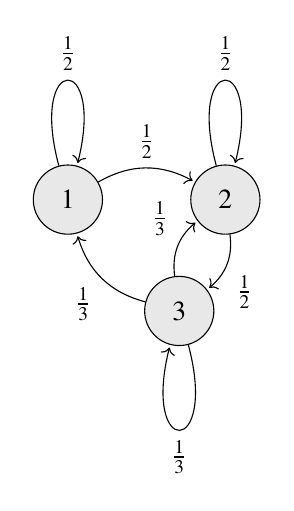
\begin{tikzpicture}[shorten >=1pt,node distance=2cm, scale =3, auto]
			\tikzstyle{every state}=[fill={rgb:black,1;white,10}]
			
			\node[state]   (q_1)                          {$1$};
			\node[state]   (q_2)  [right of=q_1]          {$2$};
			\node[state]   (q_3)  [below right of=q_1]          {$3$};
			
			\path[->]
			(q_1) edge [loop above] node {$\frac{1}{2}$}    (   )
			edge [bend left]  node {$\frac{1}{2}$}    (q_2)
			(q_2) edge [bend left]  node {$\frac{1}{2}$}    (q_3)
			edge [loop above] node {$\frac{1}{2}$}    ()
			(q_3) edge [bend left]  node {$\frac{1}{3}$}    (q_2)
			edge [bend left]  node {$\frac{1}{3}$}    (q_1)
			edge [loop below] node {$\frac{1}{3}$}    ();
		\end{tikzpicture}$
		
		\\  
		&\\
		&\\
		\hline
		\multirow{3}{*}{Checking whether the  } & \\
		& Here,\\chain is Irreducible
		& All the states are accessible to one another. \\and Aperiodic
		& $\implies$ They are in the same communication class. So, it is Irreducible.\\
		& \\
		& There exists the non- zero self-transition, which means that the chain \\
		& is Aperiodic.\\
		&\\ 
		& We know that if the Markov Chain is irreducible and aperiodic then \\
		& \qquad \qquad \qquad $\Vec{\pi}_{j} = \lim_{n \to \infty}P\{X_{n} = j\}$, $j = 1,...,N$ \\
		& These are the stationary probabilities. \\
		&\\
		\hline
		\multirow{3}{*}{Finding the Stationary} & \\
		& Stationary Probability can be represented as\\Probability Distributions
		& \qquad \qquad \qquad $\Vec{\pi} = \Vec{\pi} \vec{P}$\\
		& \\
		& \qquad $\implies$ $\myvec{v_{1}&&v_{2}&&v_{3}} = \myvec{v_{1}&&v_{2}&&v_{3}}\vec{P}$ \\
		& \\
		& Equating the above equation we get \\
		& \\
		& \qquad \qquad \qquad $\frac{1}{2}v_{1}-\frac{1}{3}v_{3} = 0$ $\label{eq:solutions/2018/dec/106/eq}$\\
		& \\
		& \qquad \qquad \qquad $\frac{1}{2}v_{1}-\frac{1}{2}v_{2} + \frac{1}{3}v_{3} = 0$\\
		& \\
		& \qquad \qquad \qquad $\frac{1}{2}v_{2}-\frac{2}{3}v_{3} = 0$\\
		& \\\
		& We see that summation of second and the third equation gives us the \\
		& first equation only. \\
		& And we know that the probability distribution will sum up to 1. \\
		& \\
		& \qquad \qquad \qquad $v_{1}+v_{2}+v_{3} = 1$ \\
		& \\
		& Therefore, we get the equation form as \\
		& \\
		& \qquad \qquad \qquad $\myvec{1&1&1\\\frac{1}{2}&0&\frac{-1}{3}\\\frac{1}{2}&\frac{-1}{2}&\frac{1}{3}}\myvec{v_{1}\\v_{2}\\v_{3}} = \myvec{1\\0\\0}$ \\
		& \\
		\hline
		\multirow{3}{*}{Solving the linear} & \\
		& The above linear equation can be solved using Gauss-Jordan method as\\equtions
		& \\
		& \qquad \qquad \qquad $\myvec{1&1&1&\vrule&1\\\frac{1}{2}&0&\frac{-1}{3}&\vrule&0\\\frac{1}{2}&\frac{-1}{2}&\frac{1}{3}&\vrule&0}$\\
		& \\
		& \qquad $\xleftrightarrow[]{R_2 \leftarrow R_2 - \frac{1}{2}R_1}$
		$\myvec{1&1&1&\vrule&1\\0&\frac{-1}{2}&\frac{-5}{6}&\vrule&\frac{-1}{2}\\\frac{1}{2}&\frac{-1}{2}&\frac{1}{3}&\vrule&0}$\\
		&\\
		& \qquad $\xleftrightarrow[]{R_3 \leftarrow R_3 - \frac{1}{2}R_1}$
		$\myvec{1&1&1&\vrule&1\\0&\frac{-1}{2}&\frac{-5}{6}&\vrule&\frac{-1}{2}\\0&-1&\frac{-1}{6}&\vrule&\frac{-1}{2}}$\\
		&\\
		& \qquad $\xleftrightarrow[]{R_2 \leftarrow \frac{-1}{2}R_2}$
		$\myvec{1&1&1&\vrule&1\\0&1&\frac{5}{3}&\vrule&1\\0&-1&\frac{-1}{6}&\vrule&\frac{-1}{2}}$\\
		&\\
		& \qquad $\xleftrightarrow[]{R_3 \leftarrow R_3 + R_2}$
		$\myvec{1&1&1&\vrule&1\\0&1&\frac{5}{3}&\vrule&1\\0&0&\frac{3}{2}&\vrule&\frac{1}{2}}$\\
		&\\
		& \qquad $\xleftrightarrow[]{R_3 \leftarrow \frac{3}{2}R_3}$
		$\myvec{1&1&1&\vrule&1\\0&1&\frac{5}{3}&\vrule&1\\0&0&1&\vrule&\frac{1}{3}}$\\
		&\\
		& \qquad $\xleftrightarrow[]{R_2 \leftarrow R_2 - \frac{5}{3}R_3}$
		$\myvec{1&1&1&\vrule&1\\0&1&0&\vrule&\frac{4}{9}\\0&0&1&\vrule&\frac{1}{3}}$\\
		&\\
		& \qquad $\xleftrightarrow[]{R_1 \leftarrow R_1 - R_3}$
		$\myvec{1&1&0&\vrule&\frac{2}{3}\\0&1&0&\vrule&\frac{4}{9}\\0&0&1&\vrule&\frac{1}{3}}$\\
		&\\
		& \qquad $\xleftrightarrow[]{R_1 \leftarrow R_1 - R_2}$
		$\myvec{1&0&0&\vrule&\frac{2}{9}\\0&1&0&\vrule&\frac{4}{9}\\0&0&1&\vrule&\frac{1}{3}}$\\
		&\\
		& $\therefore$, stationary probability distribution $\pi$ is given by \\
		& \qquad \qquad $\pi = \myvec{\frac{2}{9} & \frac{4}{9} & \frac{1}{3}}$ \\
		& \\
		\hline
		\multirow{3}{*}{Observations} & \\
		
		
		& Since the given transition probability matrix $\vec{P}$ is irreducible and aperiodic, \\
		& then $\lim_{n \to \infty} \vec{P}^{n}$ converges to a matrix with all rows identical and equal to $\vec{\pi}$. \\
		& \\
		& We were able to find $\vec{\pi}$ as $\myvec{\frac{2}{9} & \frac{4}{9} & \frac{1}{3}}$ \\
		& \\
		& $\lim_{n \to \infty} \vec{P}^{n} = \myvec{\frac{2}{9}&\frac{4}{9}&\frac{1}{3}\\\frac{2}{9}&\frac{4}{9}&\frac{1}{3}\\\frac{2}{9}&\frac{4}{9}&\frac{1}{3}}$\\
		& \\
		& From the above matrix, we get \\
		& \\
		& $\lim_{n \to \infty} \vec{P}^{n}_{11} = \frac{2}{9}$ \\
		&\\
		& $\lim_{n \to \infty} \vec{P}^{n}_{21} = \frac{2}{9}$ \\
		&\\
		& $\lim_{n \to \infty} \vec{P}^{n}_{32} = \frac{4}{9}$ \\
		&\\
		& $\lim_{n \to \infty} \vec{P}^{n}_{13} = \frac{1}{3}$ \\
		&\\
		\hline
		\multirow{3}{*}{Conclusion} & \\
		& From our observation we see that \\
		&\\
		& Options 1) and 4) are True.\\
		& \\
		\hline
\caption{}
\label{eq:solutions/2018/dec/106/table1}
	\end{longtable}
\twocolumn

\item Define a real valued function $B$ on $\mathbb{R}^2 \times \mathbb{R}^2 $ as 
\begin{align}
B\brak{\vec{x},\vec{y}} = x_1y_1 - x_1y_2-x_2y_1+4x_2y_2
\end{align}
Let $\vec{v}_0 = \myvec{1\\0}$ and 
\begin{align}
W = \cbrak{\vec{v} \in \mathbb{R}^2: B(\vec{v}_0,\vec{v}) =0}
\end{align}
Then $W$
\begin{enumerate}
\item is not a subspace of $\mathbb{R}^2$.
\item equals $\vec{0}$.
\item is the y axis
\item is the line passing through $\myvec{0 \\ 0}$ and $\myvec{1 \\ 1}$.
\end{enumerate}
%
\solution
See Tables \ref{eq:solutions/2018/dec/106/table0} and \ref{eq:solutions/2018/dec/106/table1}


\onecolumn
	\begin{longtable}{|l|l|}
		\hline
		\multirow{3}{*}{Irreducible Markov Chain} 
		& \\
		& A Markov chain is $\textbf{irreducible}$ if all the states communicate with each other,\\
		& i.e., if there is only one communication class.\\
		&\\
		\hline
		\multirow{3}{*}{Aperiodic Markov Chain} & \\
		& If there is a self-transition in the chain ($p^{ii}>0$ for some i), then the chain is\\
		& called as $\textbf{aperiodic}$\\
		& \\
		\hline
		\multirow{3}{*}{Stationary Distribution} & \\
		& A stationary distribution of a Markov chain is a probability distribution that\\
		& remains unchanged in the Markov chain as time progresses. Typically, it is\\
		& represented as a row vector $\Vec{\pi}$ whose entries are probabilities summing to 1,\\ 
		& and given transition matrix $\textbf{P}$, it satisfies\\
		& \\
		&  \qquad \qquad  \qquad$\Vec{\pi} = \Vec{\pi} \textbf{P}$\\
		& \\
		\hline
\caption{}
\label{eq:solutions/2018/dec/106/table0}
	\end{longtable}
	\begin{longtable}{|l|l|}
		\hline
		\multirow{3}{*}{Drawing Transition diagram} 
		& \\
		& 
		
		$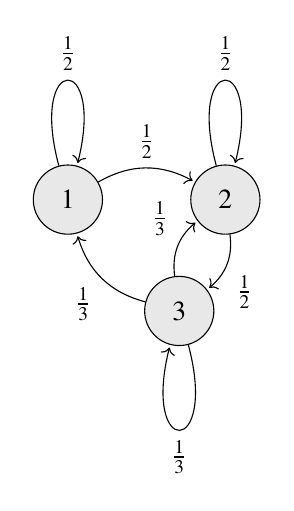
\begin{tikzpicture}[shorten >=1pt,node distance=2cm, scale =3, auto]
			\tikzstyle{every state}=[fill={rgb:black,1;white,10}]
			
			\node[state]   (q_1)                          {$1$};
			\node[state]   (q_2)  [right of=q_1]          {$2$};
			\node[state]   (q_3)  [below right of=q_1]          {$3$};
			
			\path[->]
			(q_1) edge [loop above] node {$\frac{1}{2}$}    (   )
			edge [bend left]  node {$\frac{1}{2}$}    (q_2)
			(q_2) edge [bend left]  node {$\frac{1}{2}$}    (q_3)
			edge [loop above] node {$\frac{1}{2}$}    ()
			(q_3) edge [bend left]  node {$\frac{1}{3}$}    (q_2)
			edge [bend left]  node {$\frac{1}{3}$}    (q_1)
			edge [loop below] node {$\frac{1}{3}$}    ();
		\end{tikzpicture}$
		
		\\  
		&\\
		&\\
		\hline
		\multirow{3}{*}{Checking whether the  } & \\
		& Here,\\chain is Irreducible
		& All the states are accessible to one another. \\and Aperiodic
		& $\implies$ They are in the same communication class. So, it is Irreducible.\\
		& \\
		& There exists the non- zero self-transition, which means that the chain \\
		& is Aperiodic.\\
		&\\ 
		& We know that if the Markov Chain is irreducible and aperiodic then \\
		& \qquad \qquad \qquad $\Vec{\pi}_{j} = \lim_{n \to \infty}P\{X_{n} = j\}$, $j = 1,...,N$ \\
		& These are the stationary probabilities. \\
		&\\
		\hline
		\multirow{3}{*}{Finding the Stationary} & \\
		& Stationary Probability can be represented as\\Probability Distributions
		& \qquad \qquad \qquad $\Vec{\pi} = \Vec{\pi} \vec{P}$\\
		& \\
		& \qquad $\implies$ $\myvec{v_{1}&&v_{2}&&v_{3}} = \myvec{v_{1}&&v_{2}&&v_{3}}\vec{P}$ \\
		& \\
		& Equating the above equation we get \\
		& \\
		& \qquad \qquad \qquad $\frac{1}{2}v_{1}-\frac{1}{3}v_{3} = 0$ $\label{eq:solutions/2018/dec/106/eq}$\\
		& \\
		& \qquad \qquad \qquad $\frac{1}{2}v_{1}-\frac{1}{2}v_{2} + \frac{1}{3}v_{3} = 0$\\
		& \\
		& \qquad \qquad \qquad $\frac{1}{2}v_{2}-\frac{2}{3}v_{3} = 0$\\
		& \\\
		& We see that summation of second and the third equation gives us the \\
		& first equation only. \\
		& And we know that the probability distribution will sum up to 1. \\
		& \\
		& \qquad \qquad \qquad $v_{1}+v_{2}+v_{3} = 1$ \\
		& \\
		& Therefore, we get the equation form as \\
		& \\
		& \qquad \qquad \qquad $\myvec{1&1&1\\\frac{1}{2}&0&\frac{-1}{3}\\\frac{1}{2}&\frac{-1}{2}&\frac{1}{3}}\myvec{v_{1}\\v_{2}\\v_{3}} = \myvec{1\\0\\0}$ \\
		& \\
		\hline
		\multirow{3}{*}{Solving the linear} & \\
		& The above linear equation can be solved using Gauss-Jordan method as\\equtions
		& \\
		& \qquad \qquad \qquad $\myvec{1&1&1&\vrule&1\\\frac{1}{2}&0&\frac{-1}{3}&\vrule&0\\\frac{1}{2}&\frac{-1}{2}&\frac{1}{3}&\vrule&0}$\\
		& \\
		& \qquad $\xleftrightarrow[]{R_2 \leftarrow R_2 - \frac{1}{2}R_1}$
		$\myvec{1&1&1&\vrule&1\\0&\frac{-1}{2}&\frac{-5}{6}&\vrule&\frac{-1}{2}\\\frac{1}{2}&\frac{-1}{2}&\frac{1}{3}&\vrule&0}$\\
		&\\
		& \qquad $\xleftrightarrow[]{R_3 \leftarrow R_3 - \frac{1}{2}R_1}$
		$\myvec{1&1&1&\vrule&1\\0&\frac{-1}{2}&\frac{-5}{6}&\vrule&\frac{-1}{2}\\0&-1&\frac{-1}{6}&\vrule&\frac{-1}{2}}$\\
		&\\
		& \qquad $\xleftrightarrow[]{R_2 \leftarrow \frac{-1}{2}R_2}$
		$\myvec{1&1&1&\vrule&1\\0&1&\frac{5}{3}&\vrule&1\\0&-1&\frac{-1}{6}&\vrule&\frac{-1}{2}}$\\
		&\\
		& \qquad $\xleftrightarrow[]{R_3 \leftarrow R_3 + R_2}$
		$\myvec{1&1&1&\vrule&1\\0&1&\frac{5}{3}&\vrule&1\\0&0&\frac{3}{2}&\vrule&\frac{1}{2}}$\\
		&\\
		& \qquad $\xleftrightarrow[]{R_3 \leftarrow \frac{3}{2}R_3}$
		$\myvec{1&1&1&\vrule&1\\0&1&\frac{5}{3}&\vrule&1\\0&0&1&\vrule&\frac{1}{3}}$\\
		&\\
		& \qquad $\xleftrightarrow[]{R_2 \leftarrow R_2 - \frac{5}{3}R_3}$
		$\myvec{1&1&1&\vrule&1\\0&1&0&\vrule&\frac{4}{9}\\0&0&1&\vrule&\frac{1}{3}}$\\
		&\\
		& \qquad $\xleftrightarrow[]{R_1 \leftarrow R_1 - R_3}$
		$\myvec{1&1&0&\vrule&\frac{2}{3}\\0&1&0&\vrule&\frac{4}{9}\\0&0&1&\vrule&\frac{1}{3}}$\\
		&\\
		& \qquad $\xleftrightarrow[]{R_1 \leftarrow R_1 - R_2}$
		$\myvec{1&0&0&\vrule&\frac{2}{9}\\0&1&0&\vrule&\frac{4}{9}\\0&0&1&\vrule&\frac{1}{3}}$\\
		&\\
		& $\therefore$, stationary probability distribution $\pi$ is given by \\
		& \qquad \qquad $\pi = \myvec{\frac{2}{9} & \frac{4}{9} & \frac{1}{3}}$ \\
		& \\
		\hline
		\multirow{3}{*}{Observations} & \\
		
		
		& Since the given transition probability matrix $\vec{P}$ is irreducible and aperiodic, \\
		& then $\lim_{n \to \infty} \vec{P}^{n}$ converges to a matrix with all rows identical and equal to $\vec{\pi}$. \\
		& \\
		& We were able to find $\vec{\pi}$ as $\myvec{\frac{2}{9} & \frac{4}{9} & \frac{1}{3}}$ \\
		& \\
		& $\lim_{n \to \infty} \vec{P}^{n} = \myvec{\frac{2}{9}&\frac{4}{9}&\frac{1}{3}\\\frac{2}{9}&\frac{4}{9}&\frac{1}{3}\\\frac{2}{9}&\frac{4}{9}&\frac{1}{3}}$\\
		& \\
		& From the above matrix, we get \\
		& \\
		& $\lim_{n \to \infty} \vec{P}^{n}_{11} = \frac{2}{9}$ \\
		&\\
		& $\lim_{n \to \infty} \vec{P}^{n}_{21} = \frac{2}{9}$ \\
		&\\
		& $\lim_{n \to \infty} \vec{P}^{n}_{32} = \frac{4}{9}$ \\
		&\\
		& $\lim_{n \to \infty} \vec{P}^{n}_{13} = \frac{1}{3}$ \\
		&\\
		\hline
		\multirow{3}{*}{Conclusion} & \\
		& From our observation we see that \\
		&\\
		& Options 1) and 4) are True.\\
		& \\
		\hline
\caption{}
\label{eq:solutions/2018/dec/106/table1}
	\end{longtable}
\twocolumn

\item Consider the Quadratic forms
\begin{align}
Q_1(x,y) = xy
\\
Q_2(x,y) = x^2+2xy+y^2
\\
Q_3(x,y) = x^2+3xy+2y^2
\end{align}
%
on $\mathbb{R}^2$.  Choose the correct statements from below
\begin{enumerate}
\item $Q_1$ and $Q_2$ are equivalent.
\item $Q_1$ and $Q_3$ are equivalent.
\item $Q_2$ and $Q_3$ are equivalent.
\item all are equivalent.
\end{enumerate}
\solution
See Tables \ref{eq:solutions/2018/dec/106/table0} and \ref{eq:solutions/2018/dec/106/table1}


\onecolumn
	\begin{longtable}{|l|l|}
		\hline
		\multirow{3}{*}{Irreducible Markov Chain} 
		& \\
		& A Markov chain is $\textbf{irreducible}$ if all the states communicate with each other,\\
		& i.e., if there is only one communication class.\\
		&\\
		\hline
		\multirow{3}{*}{Aperiodic Markov Chain} & \\
		& If there is a self-transition in the chain ($p^{ii}>0$ for some i), then the chain is\\
		& called as $\textbf{aperiodic}$\\
		& \\
		\hline
		\multirow{3}{*}{Stationary Distribution} & \\
		& A stationary distribution of a Markov chain is a probability distribution that\\
		& remains unchanged in the Markov chain as time progresses. Typically, it is\\
		& represented as a row vector $\Vec{\pi}$ whose entries are probabilities summing to 1,\\ 
		& and given transition matrix $\textbf{P}$, it satisfies\\
		& \\
		&  \qquad \qquad  \qquad$\Vec{\pi} = \Vec{\pi} \textbf{P}$\\
		& \\
		\hline
\caption{}
\label{eq:solutions/2018/dec/106/table0}
	\end{longtable}
	\begin{longtable}{|l|l|}
		\hline
		\multirow{3}{*}{Drawing Transition diagram} 
		& \\
		& 
		
		$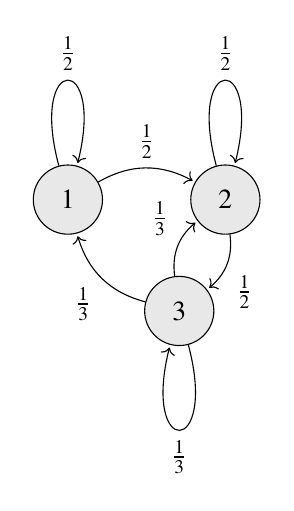
\begin{tikzpicture}[shorten >=1pt,node distance=2cm, scale =3, auto]
			\tikzstyle{every state}=[fill={rgb:black,1;white,10}]
			
			\node[state]   (q_1)                          {$1$};
			\node[state]   (q_2)  [right of=q_1]          {$2$};
			\node[state]   (q_3)  [below right of=q_1]          {$3$};
			
			\path[->]
			(q_1) edge [loop above] node {$\frac{1}{2}$}    (   )
			edge [bend left]  node {$\frac{1}{2}$}    (q_2)
			(q_2) edge [bend left]  node {$\frac{1}{2}$}    (q_3)
			edge [loop above] node {$\frac{1}{2}$}    ()
			(q_3) edge [bend left]  node {$\frac{1}{3}$}    (q_2)
			edge [bend left]  node {$\frac{1}{3}$}    (q_1)
			edge [loop below] node {$\frac{1}{3}$}    ();
		\end{tikzpicture}$
		
		\\  
		&\\
		&\\
		\hline
		\multirow{3}{*}{Checking whether the  } & \\
		& Here,\\chain is Irreducible
		& All the states are accessible to one another. \\and Aperiodic
		& $\implies$ They are in the same communication class. So, it is Irreducible.\\
		& \\
		& There exists the non- zero self-transition, which means that the chain \\
		& is Aperiodic.\\
		&\\ 
		& We know that if the Markov Chain is irreducible and aperiodic then \\
		& \qquad \qquad \qquad $\Vec{\pi}_{j} = \lim_{n \to \infty}P\{X_{n} = j\}$, $j = 1,...,N$ \\
		& These are the stationary probabilities. \\
		&\\
		\hline
		\multirow{3}{*}{Finding the Stationary} & \\
		& Stationary Probability can be represented as\\Probability Distributions
		& \qquad \qquad \qquad $\Vec{\pi} = \Vec{\pi} \vec{P}$\\
		& \\
		& \qquad $\implies$ $\myvec{v_{1}&&v_{2}&&v_{3}} = \myvec{v_{1}&&v_{2}&&v_{3}}\vec{P}$ \\
		& \\
		& Equating the above equation we get \\
		& \\
		& \qquad \qquad \qquad $\frac{1}{2}v_{1}-\frac{1}{3}v_{3} = 0$ $\label{eq:solutions/2018/dec/106/eq}$\\
		& \\
		& \qquad \qquad \qquad $\frac{1}{2}v_{1}-\frac{1}{2}v_{2} + \frac{1}{3}v_{3} = 0$\\
		& \\
		& \qquad \qquad \qquad $\frac{1}{2}v_{2}-\frac{2}{3}v_{3} = 0$\\
		& \\\
		& We see that summation of second and the third equation gives us the \\
		& first equation only. \\
		& And we know that the probability distribution will sum up to 1. \\
		& \\
		& \qquad \qquad \qquad $v_{1}+v_{2}+v_{3} = 1$ \\
		& \\
		& Therefore, we get the equation form as \\
		& \\
		& \qquad \qquad \qquad $\myvec{1&1&1\\\frac{1}{2}&0&\frac{-1}{3}\\\frac{1}{2}&\frac{-1}{2}&\frac{1}{3}}\myvec{v_{1}\\v_{2}\\v_{3}} = \myvec{1\\0\\0}$ \\
		& \\
		\hline
		\multirow{3}{*}{Solving the linear} & \\
		& The above linear equation can be solved using Gauss-Jordan method as\\equtions
		& \\
		& \qquad \qquad \qquad $\myvec{1&1&1&\vrule&1\\\frac{1}{2}&0&\frac{-1}{3}&\vrule&0\\\frac{1}{2}&\frac{-1}{2}&\frac{1}{3}&\vrule&0}$\\
		& \\
		& \qquad $\xleftrightarrow[]{R_2 \leftarrow R_2 - \frac{1}{2}R_1}$
		$\myvec{1&1&1&\vrule&1\\0&\frac{-1}{2}&\frac{-5}{6}&\vrule&\frac{-1}{2}\\\frac{1}{2}&\frac{-1}{2}&\frac{1}{3}&\vrule&0}$\\
		&\\
		& \qquad $\xleftrightarrow[]{R_3 \leftarrow R_3 - \frac{1}{2}R_1}$
		$\myvec{1&1&1&\vrule&1\\0&\frac{-1}{2}&\frac{-5}{6}&\vrule&\frac{-1}{2}\\0&-1&\frac{-1}{6}&\vrule&\frac{-1}{2}}$\\
		&\\
		& \qquad $\xleftrightarrow[]{R_2 \leftarrow \frac{-1}{2}R_2}$
		$\myvec{1&1&1&\vrule&1\\0&1&\frac{5}{3}&\vrule&1\\0&-1&\frac{-1}{6}&\vrule&\frac{-1}{2}}$\\
		&\\
		& \qquad $\xleftrightarrow[]{R_3 \leftarrow R_3 + R_2}$
		$\myvec{1&1&1&\vrule&1\\0&1&\frac{5}{3}&\vrule&1\\0&0&\frac{3}{2}&\vrule&\frac{1}{2}}$\\
		&\\
		& \qquad $\xleftrightarrow[]{R_3 \leftarrow \frac{3}{2}R_3}$
		$\myvec{1&1&1&\vrule&1\\0&1&\frac{5}{3}&\vrule&1\\0&0&1&\vrule&\frac{1}{3}}$\\
		&\\
		& \qquad $\xleftrightarrow[]{R_2 \leftarrow R_2 - \frac{5}{3}R_3}$
		$\myvec{1&1&1&\vrule&1\\0&1&0&\vrule&\frac{4}{9}\\0&0&1&\vrule&\frac{1}{3}}$\\
		&\\
		& \qquad $\xleftrightarrow[]{R_1 \leftarrow R_1 - R_3}$
		$\myvec{1&1&0&\vrule&\frac{2}{3}\\0&1&0&\vrule&\frac{4}{9}\\0&0&1&\vrule&\frac{1}{3}}$\\
		&\\
		& \qquad $\xleftrightarrow[]{R_1 \leftarrow R_1 - R_2}$
		$\myvec{1&0&0&\vrule&\frac{2}{9}\\0&1&0&\vrule&\frac{4}{9}\\0&0&1&\vrule&\frac{1}{3}}$\\
		&\\
		& $\therefore$, stationary probability distribution $\pi$ is given by \\
		& \qquad \qquad $\pi = \myvec{\frac{2}{9} & \frac{4}{9} & \frac{1}{3}}$ \\
		& \\
		\hline
		\multirow{3}{*}{Observations} & \\
		
		
		& Since the given transition probability matrix $\vec{P}$ is irreducible and aperiodic, \\
		& then $\lim_{n \to \infty} \vec{P}^{n}$ converges to a matrix with all rows identical and equal to $\vec{\pi}$. \\
		& \\
		& We were able to find $\vec{\pi}$ as $\myvec{\frac{2}{9} & \frac{4}{9} & \frac{1}{3}}$ \\
		& \\
		& $\lim_{n \to \infty} \vec{P}^{n} = \myvec{\frac{2}{9}&\frac{4}{9}&\frac{1}{3}\\\frac{2}{9}&\frac{4}{9}&\frac{1}{3}\\\frac{2}{9}&\frac{4}{9}&\frac{1}{3}}$\\
		& \\
		& From the above matrix, we get \\
		& \\
		& $\lim_{n \to \infty} \vec{P}^{n}_{11} = \frac{2}{9}$ \\
		&\\
		& $\lim_{n \to \infty} \vec{P}^{n}_{21} = \frac{2}{9}$ \\
		&\\
		& $\lim_{n \to \infty} \vec{P}^{n}_{32} = \frac{4}{9}$ \\
		&\\
		& $\lim_{n \to \infty} \vec{P}^{n}_{13} = \frac{1}{3}$ \\
		&\\
		\hline
		\multirow{3}{*}{Conclusion} & \\
		& From our observation we see that \\
		&\\
		& Options 1) and 4) are True.\\
		& \\
		\hline
\caption{}
\label{eq:solutions/2018/dec/106/table1}
	\end{longtable}
\twocolumn

\item Consider a Markov Chain with state space $\cbrak{0,1,2}$ and transition matrix
\begin{align}
P = 
\begin{blockarray}{c@{\hspace{1pt}}rrr@{\hspace{3pt}}}
         & 0   & 1   & 2 \\
        \begin{block}{r@{\hspace{3pt}}@{\hspace{1pt}}
    (@{\hspace{1pt}}rrr@{\hspace{1pt}}@{\hspace{1pt}})}
        0 & \frac{1}{2} & \frac{1}{2} & 0  \\
        1 & 0 &\frac{1}{2}  & \frac{3}{4}  \\
%
        2 &  \frac{1}{3} & \frac{1}{3} & \frac{1}{3}  \\
        \end{block}
    \end{blockarray}
\end{align}
For any two states $i$ and $j$, let $p_{ij}^{(n)}$ denote the $n$-step transition probability of going from $i$ to $j$.  Identify correct statements.
\begin{enumerate}
\item $\lim_{n \to \infty} p_{11}^{(n)} = \frac{2}{9}$
\item $\lim_{n \to \infty} p_{21}^{(n)} = 0$
\item $\lim_{n \to \infty} p_{32}^{(n)} = \frac{1}{3}$
\item $\lim_{n \to \infty} p_{13}^{(n)} = \frac{1}{3}$
\end{enumerate}
\solution
See Tables \ref{eq:solutions/2018/dec/106/table0} and \ref{eq:solutions/2018/dec/106/table1}


\onecolumn
	\begin{longtable}{|l|l|}
		\hline
		\multirow{3}{*}{Irreducible Markov Chain} 
		& \\
		& A Markov chain is $\textbf{irreducible}$ if all the states communicate with each other,\\
		& i.e., if there is only one communication class.\\
		&\\
		\hline
		\multirow{3}{*}{Aperiodic Markov Chain} & \\
		& If there is a self-transition in the chain ($p^{ii}>0$ for some i), then the chain is\\
		& called as $\textbf{aperiodic}$\\
		& \\
		\hline
		\multirow{3}{*}{Stationary Distribution} & \\
		& A stationary distribution of a Markov chain is a probability distribution that\\
		& remains unchanged in the Markov chain as time progresses. Typically, it is\\
		& represented as a row vector $\Vec{\pi}$ whose entries are probabilities summing to 1,\\ 
		& and given transition matrix $\textbf{P}$, it satisfies\\
		& \\
		&  \qquad \qquad  \qquad$\Vec{\pi} = \Vec{\pi} \textbf{P}$\\
		& \\
		\hline
\caption{}
\label{eq:solutions/2018/dec/106/table0}
	\end{longtable}
	\begin{longtable}{|l|l|}
		\hline
		\multirow{3}{*}{Drawing Transition diagram} 
		& \\
		& 
		
		$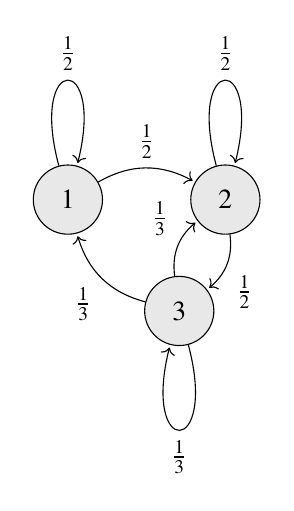
\begin{tikzpicture}[shorten >=1pt,node distance=2cm, scale =3, auto]
			\tikzstyle{every state}=[fill={rgb:black,1;white,10}]
			
			\node[state]   (q_1)                          {$1$};
			\node[state]   (q_2)  [right of=q_1]          {$2$};
			\node[state]   (q_3)  [below right of=q_1]          {$3$};
			
			\path[->]
			(q_1) edge [loop above] node {$\frac{1}{2}$}    (   )
			edge [bend left]  node {$\frac{1}{2}$}    (q_2)
			(q_2) edge [bend left]  node {$\frac{1}{2}$}    (q_3)
			edge [loop above] node {$\frac{1}{2}$}    ()
			(q_3) edge [bend left]  node {$\frac{1}{3}$}    (q_2)
			edge [bend left]  node {$\frac{1}{3}$}    (q_1)
			edge [loop below] node {$\frac{1}{3}$}    ();
		\end{tikzpicture}$
		
		\\  
		&\\
		&\\
		\hline
		\multirow{3}{*}{Checking whether the  } & \\
		& Here,\\chain is Irreducible
		& All the states are accessible to one another. \\and Aperiodic
		& $\implies$ They are in the same communication class. So, it is Irreducible.\\
		& \\
		& There exists the non- zero self-transition, which means that the chain \\
		& is Aperiodic.\\
		&\\ 
		& We know that if the Markov Chain is irreducible and aperiodic then \\
		& \qquad \qquad \qquad $\Vec{\pi}_{j} = \lim_{n \to \infty}P\{X_{n} = j\}$, $j = 1,...,N$ \\
		& These are the stationary probabilities. \\
		&\\
		\hline
		\multirow{3}{*}{Finding the Stationary} & \\
		& Stationary Probability can be represented as\\Probability Distributions
		& \qquad \qquad \qquad $\Vec{\pi} = \Vec{\pi} \vec{P}$\\
		& \\
		& \qquad $\implies$ $\myvec{v_{1}&&v_{2}&&v_{3}} = \myvec{v_{1}&&v_{2}&&v_{3}}\vec{P}$ \\
		& \\
		& Equating the above equation we get \\
		& \\
		& \qquad \qquad \qquad $\frac{1}{2}v_{1}-\frac{1}{3}v_{3} = 0$ $\label{eq:solutions/2018/dec/106/eq}$\\
		& \\
		& \qquad \qquad \qquad $\frac{1}{2}v_{1}-\frac{1}{2}v_{2} + \frac{1}{3}v_{3} = 0$\\
		& \\
		& \qquad \qquad \qquad $\frac{1}{2}v_{2}-\frac{2}{3}v_{3} = 0$\\
		& \\\
		& We see that summation of second and the third equation gives us the \\
		& first equation only. \\
		& And we know that the probability distribution will sum up to 1. \\
		& \\
		& \qquad \qquad \qquad $v_{1}+v_{2}+v_{3} = 1$ \\
		& \\
		& Therefore, we get the equation form as \\
		& \\
		& \qquad \qquad \qquad $\myvec{1&1&1\\\frac{1}{2}&0&\frac{-1}{3}\\\frac{1}{2}&\frac{-1}{2}&\frac{1}{3}}\myvec{v_{1}\\v_{2}\\v_{3}} = \myvec{1\\0\\0}$ \\
		& \\
		\hline
		\multirow{3}{*}{Solving the linear} & \\
		& The above linear equation can be solved using Gauss-Jordan method as\\equtions
		& \\
		& \qquad \qquad \qquad $\myvec{1&1&1&\vrule&1\\\frac{1}{2}&0&\frac{-1}{3}&\vrule&0\\\frac{1}{2}&\frac{-1}{2}&\frac{1}{3}&\vrule&0}$\\
		& \\
		& \qquad $\xleftrightarrow[]{R_2 \leftarrow R_2 - \frac{1}{2}R_1}$
		$\myvec{1&1&1&\vrule&1\\0&\frac{-1}{2}&\frac{-5}{6}&\vrule&\frac{-1}{2}\\\frac{1}{2}&\frac{-1}{2}&\frac{1}{3}&\vrule&0}$\\
		&\\
		& \qquad $\xleftrightarrow[]{R_3 \leftarrow R_3 - \frac{1}{2}R_1}$
		$\myvec{1&1&1&\vrule&1\\0&\frac{-1}{2}&\frac{-5}{6}&\vrule&\frac{-1}{2}\\0&-1&\frac{-1}{6}&\vrule&\frac{-1}{2}}$\\
		&\\
		& \qquad $\xleftrightarrow[]{R_2 \leftarrow \frac{-1}{2}R_2}$
		$\myvec{1&1&1&\vrule&1\\0&1&\frac{5}{3}&\vrule&1\\0&-1&\frac{-1}{6}&\vrule&\frac{-1}{2}}$\\
		&\\
		& \qquad $\xleftrightarrow[]{R_3 \leftarrow R_3 + R_2}$
		$\myvec{1&1&1&\vrule&1\\0&1&\frac{5}{3}&\vrule&1\\0&0&\frac{3}{2}&\vrule&\frac{1}{2}}$\\
		&\\
		& \qquad $\xleftrightarrow[]{R_3 \leftarrow \frac{3}{2}R_3}$
		$\myvec{1&1&1&\vrule&1\\0&1&\frac{5}{3}&\vrule&1\\0&0&1&\vrule&\frac{1}{3}}$\\
		&\\
		& \qquad $\xleftrightarrow[]{R_2 \leftarrow R_2 - \frac{5}{3}R_3}$
		$\myvec{1&1&1&\vrule&1\\0&1&0&\vrule&\frac{4}{9}\\0&0&1&\vrule&\frac{1}{3}}$\\
		&\\
		& \qquad $\xleftrightarrow[]{R_1 \leftarrow R_1 - R_3}$
		$\myvec{1&1&0&\vrule&\frac{2}{3}\\0&1&0&\vrule&\frac{4}{9}\\0&0&1&\vrule&\frac{1}{3}}$\\
		&\\
		& \qquad $\xleftrightarrow[]{R_1 \leftarrow R_1 - R_2}$
		$\myvec{1&0&0&\vrule&\frac{2}{9}\\0&1&0&\vrule&\frac{4}{9}\\0&0&1&\vrule&\frac{1}{3}}$\\
		&\\
		& $\therefore$, stationary probability distribution $\pi$ is given by \\
		& \qquad \qquad $\pi = \myvec{\frac{2}{9} & \frac{4}{9} & \frac{1}{3}}$ \\
		& \\
		\hline
		\multirow{3}{*}{Observations} & \\
		
		
		& Since the given transition probability matrix $\vec{P}$ is irreducible and aperiodic, \\
		& then $\lim_{n \to \infty} \vec{P}^{n}$ converges to a matrix with all rows identical and equal to $\vec{\pi}$. \\
		& \\
		& We were able to find $\vec{\pi}$ as $\myvec{\frac{2}{9} & \frac{4}{9} & \frac{1}{3}}$ \\
		& \\
		& $\lim_{n \to \infty} \vec{P}^{n} = \myvec{\frac{2}{9}&\frac{4}{9}&\frac{1}{3}\\\frac{2}{9}&\frac{4}{9}&\frac{1}{3}\\\frac{2}{9}&\frac{4}{9}&\frac{1}{3}}$\\
		& \\
		& From the above matrix, we get \\
		& \\
		& $\lim_{n \to \infty} \vec{P}^{n}_{11} = \frac{2}{9}$ \\
		&\\
		& $\lim_{n \to \infty} \vec{P}^{n}_{21} = \frac{2}{9}$ \\
		&\\
		& $\lim_{n \to \infty} \vec{P}^{n}_{32} = \frac{4}{9}$ \\
		&\\
		& $\lim_{n \to \infty} \vec{P}^{n}_{13} = \frac{1}{3}$ \\
		&\\
		\hline
		\multirow{3}{*}{Conclusion} & \\
		& From our observation we see that \\
		&\\
		& Options 1) and 4) are True.\\
		& \\
		\hline
\caption{}
\label{eq:solutions/2018/dec/106/table1}
	\end{longtable}
\twocolumn


\end{enumerate}

\section{June 2018}
\renewcommand{\theequation}{\theenumi}
\renewcommand{\thefigure}{\theenumi}
\begin{enumerate}[label=\thesection.\arabic*.,ref=\thesection.\theenumi]
\numberwithin{equation}{enumi}
\numberwithin{figure}{enumi}

\item 	Let $\vec{A}$ be a $4 \times 4$ matrix. Suppose that the null space $N(\vec{A})$ of $\vec{A}$ is
	\begin{align}
		\cbrak{(x,y,z,w) \in \vec{R}^4 : x + y + z = 0 , x + y + w = 0}
	\end{align}
Then which one of the following is correct
\begin{enumerate}
\item  dim(column space$(\vec{A})) = 1$ 
\item dim(column space$(\vec{A})) = 2$
\item rank$(\vec{A}) = 1$
\item $\vec{S}= \cbrak{(1, 1, 1, 0), (1, 1, 0, 1)}$ is a basis of $N(\vec{A})$
\end{enumerate}
%
%
\solution
See Tables \ref{eq:solutions/2018/dec/106/table0} and \ref{eq:solutions/2018/dec/106/table1}


\onecolumn
	\begin{longtable}{|l|l|}
		\hline
		\multirow{3}{*}{Irreducible Markov Chain} 
		& \\
		& A Markov chain is $\textbf{irreducible}$ if all the states communicate with each other,\\
		& i.e., if there is only one communication class.\\
		&\\
		\hline
		\multirow{3}{*}{Aperiodic Markov Chain} & \\
		& If there is a self-transition in the chain ($p^{ii}>0$ for some i), then the chain is\\
		& called as $\textbf{aperiodic}$\\
		& \\
		\hline
		\multirow{3}{*}{Stationary Distribution} & \\
		& A stationary distribution of a Markov chain is a probability distribution that\\
		& remains unchanged in the Markov chain as time progresses. Typically, it is\\
		& represented as a row vector $\Vec{\pi}$ whose entries are probabilities summing to 1,\\ 
		& and given transition matrix $\textbf{P}$, it satisfies\\
		& \\
		&  \qquad \qquad  \qquad$\Vec{\pi} = \Vec{\pi} \textbf{P}$\\
		& \\
		\hline
\caption{}
\label{eq:solutions/2018/dec/106/table0}
	\end{longtable}
	\begin{longtable}{|l|l|}
		\hline
		\multirow{3}{*}{Drawing Transition diagram} 
		& \\
		& 
		
		$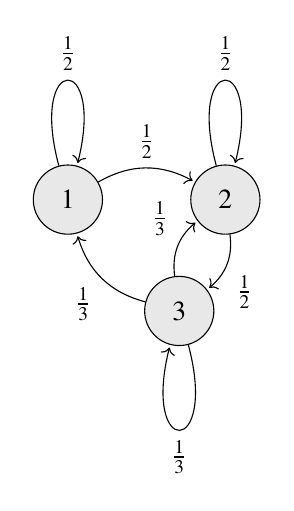
\begin{tikzpicture}[shorten >=1pt,node distance=2cm, scale =3, auto]
			\tikzstyle{every state}=[fill={rgb:black,1;white,10}]
			
			\node[state]   (q_1)                          {$1$};
			\node[state]   (q_2)  [right of=q_1]          {$2$};
			\node[state]   (q_3)  [below right of=q_1]          {$3$};
			
			\path[->]
			(q_1) edge [loop above] node {$\frac{1}{2}$}    (   )
			edge [bend left]  node {$\frac{1}{2}$}    (q_2)
			(q_2) edge [bend left]  node {$\frac{1}{2}$}    (q_3)
			edge [loop above] node {$\frac{1}{2}$}    ()
			(q_3) edge [bend left]  node {$\frac{1}{3}$}    (q_2)
			edge [bend left]  node {$\frac{1}{3}$}    (q_1)
			edge [loop below] node {$\frac{1}{3}$}    ();
		\end{tikzpicture}$
		
		\\  
		&\\
		&\\
		\hline
		\multirow{3}{*}{Checking whether the  } & \\
		& Here,\\chain is Irreducible
		& All the states are accessible to one another. \\and Aperiodic
		& $\implies$ They are in the same communication class. So, it is Irreducible.\\
		& \\
		& There exists the non- zero self-transition, which means that the chain \\
		& is Aperiodic.\\
		&\\ 
		& We know that if the Markov Chain is irreducible and aperiodic then \\
		& \qquad \qquad \qquad $\Vec{\pi}_{j} = \lim_{n \to \infty}P\{X_{n} = j\}$, $j = 1,...,N$ \\
		& These are the stationary probabilities. \\
		&\\
		\hline
		\multirow{3}{*}{Finding the Stationary} & \\
		& Stationary Probability can be represented as\\Probability Distributions
		& \qquad \qquad \qquad $\Vec{\pi} = \Vec{\pi} \vec{P}$\\
		& \\
		& \qquad $\implies$ $\myvec{v_{1}&&v_{2}&&v_{3}} = \myvec{v_{1}&&v_{2}&&v_{3}}\vec{P}$ \\
		& \\
		& Equating the above equation we get \\
		& \\
		& \qquad \qquad \qquad $\frac{1}{2}v_{1}-\frac{1}{3}v_{3} = 0$ $\label{eq:solutions/2018/dec/106/eq}$\\
		& \\
		& \qquad \qquad \qquad $\frac{1}{2}v_{1}-\frac{1}{2}v_{2} + \frac{1}{3}v_{3} = 0$\\
		& \\
		& \qquad \qquad \qquad $\frac{1}{2}v_{2}-\frac{2}{3}v_{3} = 0$\\
		& \\\
		& We see that summation of second and the third equation gives us the \\
		& first equation only. \\
		& And we know that the probability distribution will sum up to 1. \\
		& \\
		& \qquad \qquad \qquad $v_{1}+v_{2}+v_{3} = 1$ \\
		& \\
		& Therefore, we get the equation form as \\
		& \\
		& \qquad \qquad \qquad $\myvec{1&1&1\\\frac{1}{2}&0&\frac{-1}{3}\\\frac{1}{2}&\frac{-1}{2}&\frac{1}{3}}\myvec{v_{1}\\v_{2}\\v_{3}} = \myvec{1\\0\\0}$ \\
		& \\
		\hline
		\multirow{3}{*}{Solving the linear} & \\
		& The above linear equation can be solved using Gauss-Jordan method as\\equtions
		& \\
		& \qquad \qquad \qquad $\myvec{1&1&1&\vrule&1\\\frac{1}{2}&0&\frac{-1}{3}&\vrule&0\\\frac{1}{2}&\frac{-1}{2}&\frac{1}{3}&\vrule&0}$\\
		& \\
		& \qquad $\xleftrightarrow[]{R_2 \leftarrow R_2 - \frac{1}{2}R_1}$
		$\myvec{1&1&1&\vrule&1\\0&\frac{-1}{2}&\frac{-5}{6}&\vrule&\frac{-1}{2}\\\frac{1}{2}&\frac{-1}{2}&\frac{1}{3}&\vrule&0}$\\
		&\\
		& \qquad $\xleftrightarrow[]{R_3 \leftarrow R_3 - \frac{1}{2}R_1}$
		$\myvec{1&1&1&\vrule&1\\0&\frac{-1}{2}&\frac{-5}{6}&\vrule&\frac{-1}{2}\\0&-1&\frac{-1}{6}&\vrule&\frac{-1}{2}}$\\
		&\\
		& \qquad $\xleftrightarrow[]{R_2 \leftarrow \frac{-1}{2}R_2}$
		$\myvec{1&1&1&\vrule&1\\0&1&\frac{5}{3}&\vrule&1\\0&-1&\frac{-1}{6}&\vrule&\frac{-1}{2}}$\\
		&\\
		& \qquad $\xleftrightarrow[]{R_3 \leftarrow R_3 + R_2}$
		$\myvec{1&1&1&\vrule&1\\0&1&\frac{5}{3}&\vrule&1\\0&0&\frac{3}{2}&\vrule&\frac{1}{2}}$\\
		&\\
		& \qquad $\xleftrightarrow[]{R_3 \leftarrow \frac{3}{2}R_3}$
		$\myvec{1&1&1&\vrule&1\\0&1&\frac{5}{3}&\vrule&1\\0&0&1&\vrule&\frac{1}{3}}$\\
		&\\
		& \qquad $\xleftrightarrow[]{R_2 \leftarrow R_2 - \frac{5}{3}R_3}$
		$\myvec{1&1&1&\vrule&1\\0&1&0&\vrule&\frac{4}{9}\\0&0&1&\vrule&\frac{1}{3}}$\\
		&\\
		& \qquad $\xleftrightarrow[]{R_1 \leftarrow R_1 - R_3}$
		$\myvec{1&1&0&\vrule&\frac{2}{3}\\0&1&0&\vrule&\frac{4}{9}\\0&0&1&\vrule&\frac{1}{3}}$\\
		&\\
		& \qquad $\xleftrightarrow[]{R_1 \leftarrow R_1 - R_2}$
		$\myvec{1&0&0&\vrule&\frac{2}{9}\\0&1&0&\vrule&\frac{4}{9}\\0&0&1&\vrule&\frac{1}{3}}$\\
		&\\
		& $\therefore$, stationary probability distribution $\pi$ is given by \\
		& \qquad \qquad $\pi = \myvec{\frac{2}{9} & \frac{4}{9} & \frac{1}{3}}$ \\
		& \\
		\hline
		\multirow{3}{*}{Observations} & \\
		
		
		& Since the given transition probability matrix $\vec{P}$ is irreducible and aperiodic, \\
		& then $\lim_{n \to \infty} \vec{P}^{n}$ converges to a matrix with all rows identical and equal to $\vec{\pi}$. \\
		& \\
		& We were able to find $\vec{\pi}$ as $\myvec{\frac{2}{9} & \frac{4}{9} & \frac{1}{3}}$ \\
		& \\
		& $\lim_{n \to \infty} \vec{P}^{n} = \myvec{\frac{2}{9}&\frac{4}{9}&\frac{1}{3}\\\frac{2}{9}&\frac{4}{9}&\frac{1}{3}\\\frac{2}{9}&\frac{4}{9}&\frac{1}{3}}$\\
		& \\
		& From the above matrix, we get \\
		& \\
		& $\lim_{n \to \infty} \vec{P}^{n}_{11} = \frac{2}{9}$ \\
		&\\
		& $\lim_{n \to \infty} \vec{P}^{n}_{21} = \frac{2}{9}$ \\
		&\\
		& $\lim_{n \to \infty} \vec{P}^{n}_{32} = \frac{4}{9}$ \\
		&\\
		& $\lim_{n \to \infty} \vec{P}^{n}_{13} = \frac{1}{3}$ \\
		&\\
		\hline
		\multirow{3}{*}{Conclusion} & \\
		& From our observation we see that \\
		&\\
		& Options 1) and 4) are True.\\
		& \\
		\hline
\caption{}
\label{eq:solutions/2018/dec/106/table1}
	\end{longtable}
\twocolumn

\item Let $\vec{A}$ and $\vec{B}$ be real invertible matrices such that 
\begin{align}
    \vec{AB}=-\vec{BA}\label{eq:eq:solutions/2017/june/28/eq1}.
\end{align}
Then
\begin{enumerate}
    \item trace{$\vec{A}$} = trace($\vec{B}$) = 0
    \item trace{$\vec{A}$} = trace($\vec{B}$) = 1
    \item trace{$\vec{A}$} = 0, trace($\vec{B}$) = 1
    \item trace($\vec{A}$) = 1, trace($\vec{B}$) = 0
\end{enumerate}
%
\solution
See Tables \ref{eq:solutions/2018/dec/106/table0} and \ref{eq:solutions/2018/dec/106/table1}


\onecolumn
	\begin{longtable}{|l|l|}
		\hline
		\multirow{3}{*}{Irreducible Markov Chain} 
		& \\
		& A Markov chain is $\textbf{irreducible}$ if all the states communicate with each other,\\
		& i.e., if there is only one communication class.\\
		&\\
		\hline
		\multirow{3}{*}{Aperiodic Markov Chain} & \\
		& If there is a self-transition in the chain ($p^{ii}>0$ for some i), then the chain is\\
		& called as $\textbf{aperiodic}$\\
		& \\
		\hline
		\multirow{3}{*}{Stationary Distribution} & \\
		& A stationary distribution of a Markov chain is a probability distribution that\\
		& remains unchanged in the Markov chain as time progresses. Typically, it is\\
		& represented as a row vector $\Vec{\pi}$ whose entries are probabilities summing to 1,\\ 
		& and given transition matrix $\textbf{P}$, it satisfies\\
		& \\
		&  \qquad \qquad  \qquad$\Vec{\pi} = \Vec{\pi} \textbf{P}$\\
		& \\
		\hline
\caption{}
\label{eq:solutions/2018/dec/106/table0}
	\end{longtable}
	\begin{longtable}{|l|l|}
		\hline
		\multirow{3}{*}{Drawing Transition diagram} 
		& \\
		& 
		
		$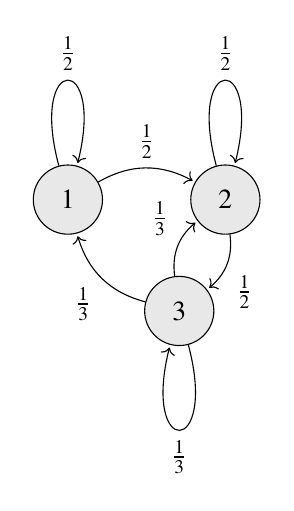
\begin{tikzpicture}[shorten >=1pt,node distance=2cm, scale =3, auto]
			\tikzstyle{every state}=[fill={rgb:black,1;white,10}]
			
			\node[state]   (q_1)                          {$1$};
			\node[state]   (q_2)  [right of=q_1]          {$2$};
			\node[state]   (q_3)  [below right of=q_1]          {$3$};
			
			\path[->]
			(q_1) edge [loop above] node {$\frac{1}{2}$}    (   )
			edge [bend left]  node {$\frac{1}{2}$}    (q_2)
			(q_2) edge [bend left]  node {$\frac{1}{2}$}    (q_3)
			edge [loop above] node {$\frac{1}{2}$}    ()
			(q_3) edge [bend left]  node {$\frac{1}{3}$}    (q_2)
			edge [bend left]  node {$\frac{1}{3}$}    (q_1)
			edge [loop below] node {$\frac{1}{3}$}    ();
		\end{tikzpicture}$
		
		\\  
		&\\
		&\\
		\hline
		\multirow{3}{*}{Checking whether the  } & \\
		& Here,\\chain is Irreducible
		& All the states are accessible to one another. \\and Aperiodic
		& $\implies$ They are in the same communication class. So, it is Irreducible.\\
		& \\
		& There exists the non- zero self-transition, which means that the chain \\
		& is Aperiodic.\\
		&\\ 
		& We know that if the Markov Chain is irreducible and aperiodic then \\
		& \qquad \qquad \qquad $\Vec{\pi}_{j} = \lim_{n \to \infty}P\{X_{n} = j\}$, $j = 1,...,N$ \\
		& These are the stationary probabilities. \\
		&\\
		\hline
		\multirow{3}{*}{Finding the Stationary} & \\
		& Stationary Probability can be represented as\\Probability Distributions
		& \qquad \qquad \qquad $\Vec{\pi} = \Vec{\pi} \vec{P}$\\
		& \\
		& \qquad $\implies$ $\myvec{v_{1}&&v_{2}&&v_{3}} = \myvec{v_{1}&&v_{2}&&v_{3}}\vec{P}$ \\
		& \\
		& Equating the above equation we get \\
		& \\
		& \qquad \qquad \qquad $\frac{1}{2}v_{1}-\frac{1}{3}v_{3} = 0$ $\label{eq:solutions/2018/dec/106/eq}$\\
		& \\
		& \qquad \qquad \qquad $\frac{1}{2}v_{1}-\frac{1}{2}v_{2} + \frac{1}{3}v_{3} = 0$\\
		& \\
		& \qquad \qquad \qquad $\frac{1}{2}v_{2}-\frac{2}{3}v_{3} = 0$\\
		& \\\
		& We see that summation of second and the third equation gives us the \\
		& first equation only. \\
		& And we know that the probability distribution will sum up to 1. \\
		& \\
		& \qquad \qquad \qquad $v_{1}+v_{2}+v_{3} = 1$ \\
		& \\
		& Therefore, we get the equation form as \\
		& \\
		& \qquad \qquad \qquad $\myvec{1&1&1\\\frac{1}{2}&0&\frac{-1}{3}\\\frac{1}{2}&\frac{-1}{2}&\frac{1}{3}}\myvec{v_{1}\\v_{2}\\v_{3}} = \myvec{1\\0\\0}$ \\
		& \\
		\hline
		\multirow{3}{*}{Solving the linear} & \\
		& The above linear equation can be solved using Gauss-Jordan method as\\equtions
		& \\
		& \qquad \qquad \qquad $\myvec{1&1&1&\vrule&1\\\frac{1}{2}&0&\frac{-1}{3}&\vrule&0\\\frac{1}{2}&\frac{-1}{2}&\frac{1}{3}&\vrule&0}$\\
		& \\
		& \qquad $\xleftrightarrow[]{R_2 \leftarrow R_2 - \frac{1}{2}R_1}$
		$\myvec{1&1&1&\vrule&1\\0&\frac{-1}{2}&\frac{-5}{6}&\vrule&\frac{-1}{2}\\\frac{1}{2}&\frac{-1}{2}&\frac{1}{3}&\vrule&0}$\\
		&\\
		& \qquad $\xleftrightarrow[]{R_3 \leftarrow R_3 - \frac{1}{2}R_1}$
		$\myvec{1&1&1&\vrule&1\\0&\frac{-1}{2}&\frac{-5}{6}&\vrule&\frac{-1}{2}\\0&-1&\frac{-1}{6}&\vrule&\frac{-1}{2}}$\\
		&\\
		& \qquad $\xleftrightarrow[]{R_2 \leftarrow \frac{-1}{2}R_2}$
		$\myvec{1&1&1&\vrule&1\\0&1&\frac{5}{3}&\vrule&1\\0&-1&\frac{-1}{6}&\vrule&\frac{-1}{2}}$\\
		&\\
		& \qquad $\xleftrightarrow[]{R_3 \leftarrow R_3 + R_2}$
		$\myvec{1&1&1&\vrule&1\\0&1&\frac{5}{3}&\vrule&1\\0&0&\frac{3}{2}&\vrule&\frac{1}{2}}$\\
		&\\
		& \qquad $\xleftrightarrow[]{R_3 \leftarrow \frac{3}{2}R_3}$
		$\myvec{1&1&1&\vrule&1\\0&1&\frac{5}{3}&\vrule&1\\0&0&1&\vrule&\frac{1}{3}}$\\
		&\\
		& \qquad $\xleftrightarrow[]{R_2 \leftarrow R_2 - \frac{5}{3}R_3}$
		$\myvec{1&1&1&\vrule&1\\0&1&0&\vrule&\frac{4}{9}\\0&0&1&\vrule&\frac{1}{3}}$\\
		&\\
		& \qquad $\xleftrightarrow[]{R_1 \leftarrow R_1 - R_3}$
		$\myvec{1&1&0&\vrule&\frac{2}{3}\\0&1&0&\vrule&\frac{4}{9}\\0&0&1&\vrule&\frac{1}{3}}$\\
		&\\
		& \qquad $\xleftrightarrow[]{R_1 \leftarrow R_1 - R_2}$
		$\myvec{1&0&0&\vrule&\frac{2}{9}\\0&1&0&\vrule&\frac{4}{9}\\0&0&1&\vrule&\frac{1}{3}}$\\
		&\\
		& $\therefore$, stationary probability distribution $\pi$ is given by \\
		& \qquad \qquad $\pi = \myvec{\frac{2}{9} & \frac{4}{9} & \frac{1}{3}}$ \\
		& \\
		\hline
		\multirow{3}{*}{Observations} & \\
		
		
		& Since the given transition probability matrix $\vec{P}$ is irreducible and aperiodic, \\
		& then $\lim_{n \to \infty} \vec{P}^{n}$ converges to a matrix with all rows identical and equal to $\vec{\pi}$. \\
		& \\
		& We were able to find $\vec{\pi}$ as $\myvec{\frac{2}{9} & \frac{4}{9} & \frac{1}{3}}$ \\
		& \\
		& $\lim_{n \to \infty} \vec{P}^{n} = \myvec{\frac{2}{9}&\frac{4}{9}&\frac{1}{3}\\\frac{2}{9}&\frac{4}{9}&\frac{1}{3}\\\frac{2}{9}&\frac{4}{9}&\frac{1}{3}}$\\
		& \\
		& From the above matrix, we get \\
		& \\
		& $\lim_{n \to \infty} \vec{P}^{n}_{11} = \frac{2}{9}$ \\
		&\\
		& $\lim_{n \to \infty} \vec{P}^{n}_{21} = \frac{2}{9}$ \\
		&\\
		& $\lim_{n \to \infty} \vec{P}^{n}_{32} = \frac{4}{9}$ \\
		&\\
		& $\lim_{n \to \infty} \vec{P}^{n}_{13} = \frac{1}{3}$ \\
		&\\
		\hline
		\multirow{3}{*}{Conclusion} & \\
		& From our observation we see that \\
		&\\
		& Options 1) and 4) are True.\\
		& \\
		\hline
\caption{}
\label{eq:solutions/2018/dec/106/table1}
	\end{longtable}
\twocolumn

\item Let $\vec{A}$ be an n $\times$ n self-adjoint matrix with eigenvalues $\lambda_1, \cdots, \lambda_2$.
Let,\begin{align} \norm{\vec{X}}_2=\sqrt{\vert\vec{X}_{1}^{2}\vert+\cdots+\vert\vec{X}_{n}^{2}\vert}\end{align} for $\vec{X}$=$(\vec{X}_{1},\cdots,\vec{X}_{n})\in \mathbb{C}^n$. If \begin{align}
p(\vec{A})=a_0\vec{I}+a_1\vec{A}+\cdots+a_n\vec{A}^n
\end{align}
then $sup_{\norm{\vec{X}}_{2}=1}\norm{p(\vec{A})\vec{X}}_2$ is equal to
%
\\
\solution
See Tables \ref{eq:solutions/2018/dec/106/table0} and \ref{eq:solutions/2018/dec/106/table1}


\onecolumn
	\begin{longtable}{|l|l|}
		\hline
		\multirow{3}{*}{Irreducible Markov Chain} 
		& \\
		& A Markov chain is $\textbf{irreducible}$ if all the states communicate with each other,\\
		& i.e., if there is only one communication class.\\
		&\\
		\hline
		\multirow{3}{*}{Aperiodic Markov Chain} & \\
		& If there is a self-transition in the chain ($p^{ii}>0$ for some i), then the chain is\\
		& called as $\textbf{aperiodic}$\\
		& \\
		\hline
		\multirow{3}{*}{Stationary Distribution} & \\
		& A stationary distribution of a Markov chain is a probability distribution that\\
		& remains unchanged in the Markov chain as time progresses. Typically, it is\\
		& represented as a row vector $\Vec{\pi}$ whose entries are probabilities summing to 1,\\ 
		& and given transition matrix $\textbf{P}$, it satisfies\\
		& \\
		&  \qquad \qquad  \qquad$\Vec{\pi} = \Vec{\pi} \textbf{P}$\\
		& \\
		\hline
\caption{}
\label{eq:solutions/2018/dec/106/table0}
	\end{longtable}
	\begin{longtable}{|l|l|}
		\hline
		\multirow{3}{*}{Drawing Transition diagram} 
		& \\
		& 
		
		$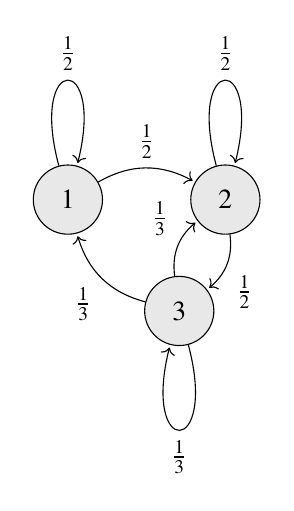
\begin{tikzpicture}[shorten >=1pt,node distance=2cm, scale =3, auto]
			\tikzstyle{every state}=[fill={rgb:black,1;white,10}]
			
			\node[state]   (q_1)                          {$1$};
			\node[state]   (q_2)  [right of=q_1]          {$2$};
			\node[state]   (q_3)  [below right of=q_1]          {$3$};
			
			\path[->]
			(q_1) edge [loop above] node {$\frac{1}{2}$}    (   )
			edge [bend left]  node {$\frac{1}{2}$}    (q_2)
			(q_2) edge [bend left]  node {$\frac{1}{2}$}    (q_3)
			edge [loop above] node {$\frac{1}{2}$}    ()
			(q_3) edge [bend left]  node {$\frac{1}{3}$}    (q_2)
			edge [bend left]  node {$\frac{1}{3}$}    (q_1)
			edge [loop below] node {$\frac{1}{3}$}    ();
		\end{tikzpicture}$
		
		\\  
		&\\
		&\\
		\hline
		\multirow{3}{*}{Checking whether the  } & \\
		& Here,\\chain is Irreducible
		& All the states are accessible to one another. \\and Aperiodic
		& $\implies$ They are in the same communication class. So, it is Irreducible.\\
		& \\
		& There exists the non- zero self-transition, which means that the chain \\
		& is Aperiodic.\\
		&\\ 
		& We know that if the Markov Chain is irreducible and aperiodic then \\
		& \qquad \qquad \qquad $\Vec{\pi}_{j} = \lim_{n \to \infty}P\{X_{n} = j\}$, $j = 1,...,N$ \\
		& These are the stationary probabilities. \\
		&\\
		\hline
		\multirow{3}{*}{Finding the Stationary} & \\
		& Stationary Probability can be represented as\\Probability Distributions
		& \qquad \qquad \qquad $\Vec{\pi} = \Vec{\pi} \vec{P}$\\
		& \\
		& \qquad $\implies$ $\myvec{v_{1}&&v_{2}&&v_{3}} = \myvec{v_{1}&&v_{2}&&v_{3}}\vec{P}$ \\
		& \\
		& Equating the above equation we get \\
		& \\
		& \qquad \qquad \qquad $\frac{1}{2}v_{1}-\frac{1}{3}v_{3} = 0$ $\label{eq:solutions/2018/dec/106/eq}$\\
		& \\
		& \qquad \qquad \qquad $\frac{1}{2}v_{1}-\frac{1}{2}v_{2} + \frac{1}{3}v_{3} = 0$\\
		& \\
		& \qquad \qquad \qquad $\frac{1}{2}v_{2}-\frac{2}{3}v_{3} = 0$\\
		& \\\
		& We see that summation of second and the third equation gives us the \\
		& first equation only. \\
		& And we know that the probability distribution will sum up to 1. \\
		& \\
		& \qquad \qquad \qquad $v_{1}+v_{2}+v_{3} = 1$ \\
		& \\
		& Therefore, we get the equation form as \\
		& \\
		& \qquad \qquad \qquad $\myvec{1&1&1\\\frac{1}{2}&0&\frac{-1}{3}\\\frac{1}{2}&\frac{-1}{2}&\frac{1}{3}}\myvec{v_{1}\\v_{2}\\v_{3}} = \myvec{1\\0\\0}$ \\
		& \\
		\hline
		\multirow{3}{*}{Solving the linear} & \\
		& The above linear equation can be solved using Gauss-Jordan method as\\equtions
		& \\
		& \qquad \qquad \qquad $\myvec{1&1&1&\vrule&1\\\frac{1}{2}&0&\frac{-1}{3}&\vrule&0\\\frac{1}{2}&\frac{-1}{2}&\frac{1}{3}&\vrule&0}$\\
		& \\
		& \qquad $\xleftrightarrow[]{R_2 \leftarrow R_2 - \frac{1}{2}R_1}$
		$\myvec{1&1&1&\vrule&1\\0&\frac{-1}{2}&\frac{-5}{6}&\vrule&\frac{-1}{2}\\\frac{1}{2}&\frac{-1}{2}&\frac{1}{3}&\vrule&0}$\\
		&\\
		& \qquad $\xleftrightarrow[]{R_3 \leftarrow R_3 - \frac{1}{2}R_1}$
		$\myvec{1&1&1&\vrule&1\\0&\frac{-1}{2}&\frac{-5}{6}&\vrule&\frac{-1}{2}\\0&-1&\frac{-1}{6}&\vrule&\frac{-1}{2}}$\\
		&\\
		& \qquad $\xleftrightarrow[]{R_2 \leftarrow \frac{-1}{2}R_2}$
		$\myvec{1&1&1&\vrule&1\\0&1&\frac{5}{3}&\vrule&1\\0&-1&\frac{-1}{6}&\vrule&\frac{-1}{2}}$\\
		&\\
		& \qquad $\xleftrightarrow[]{R_3 \leftarrow R_3 + R_2}$
		$\myvec{1&1&1&\vrule&1\\0&1&\frac{5}{3}&\vrule&1\\0&0&\frac{3}{2}&\vrule&\frac{1}{2}}$\\
		&\\
		& \qquad $\xleftrightarrow[]{R_3 \leftarrow \frac{3}{2}R_3}$
		$\myvec{1&1&1&\vrule&1\\0&1&\frac{5}{3}&\vrule&1\\0&0&1&\vrule&\frac{1}{3}}$\\
		&\\
		& \qquad $\xleftrightarrow[]{R_2 \leftarrow R_2 - \frac{5}{3}R_3}$
		$\myvec{1&1&1&\vrule&1\\0&1&0&\vrule&\frac{4}{9}\\0&0&1&\vrule&\frac{1}{3}}$\\
		&\\
		& \qquad $\xleftrightarrow[]{R_1 \leftarrow R_1 - R_3}$
		$\myvec{1&1&0&\vrule&\frac{2}{3}\\0&1&0&\vrule&\frac{4}{9}\\0&0&1&\vrule&\frac{1}{3}}$\\
		&\\
		& \qquad $\xleftrightarrow[]{R_1 \leftarrow R_1 - R_2}$
		$\myvec{1&0&0&\vrule&\frac{2}{9}\\0&1&0&\vrule&\frac{4}{9}\\0&0&1&\vrule&\frac{1}{3}}$\\
		&\\
		& $\therefore$, stationary probability distribution $\pi$ is given by \\
		& \qquad \qquad $\pi = \myvec{\frac{2}{9} & \frac{4}{9} & \frac{1}{3}}$ \\
		& \\
		\hline
		\multirow{3}{*}{Observations} & \\
		
		
		& Since the given transition probability matrix $\vec{P}$ is irreducible and aperiodic, \\
		& then $\lim_{n \to \infty} \vec{P}^{n}$ converges to a matrix with all rows identical and equal to $\vec{\pi}$. \\
		& \\
		& We were able to find $\vec{\pi}$ as $\myvec{\frac{2}{9} & \frac{4}{9} & \frac{1}{3}}$ \\
		& \\
		& $\lim_{n \to \infty} \vec{P}^{n} = \myvec{\frac{2}{9}&\frac{4}{9}&\frac{1}{3}\\\frac{2}{9}&\frac{4}{9}&\frac{1}{3}\\\frac{2}{9}&\frac{4}{9}&\frac{1}{3}}$\\
		& \\
		& From the above matrix, we get \\
		& \\
		& $\lim_{n \to \infty} \vec{P}^{n}_{11} = \frac{2}{9}$ \\
		&\\
		& $\lim_{n \to \infty} \vec{P}^{n}_{21} = \frac{2}{9}$ \\
		&\\
		& $\lim_{n \to \infty} \vec{P}^{n}_{32} = \frac{4}{9}$ \\
		&\\
		& $\lim_{n \to \infty} \vec{P}^{n}_{13} = \frac{1}{3}$ \\
		&\\
		\hline
		\multirow{3}{*}{Conclusion} & \\
		& From our observation we see that \\
		&\\
		& Options 1) and 4) are True.\\
		& \\
		\hline
\caption{}
\label{eq:solutions/2018/dec/106/table1}
	\end{longtable}
\twocolumn

\item Let $p \brak{x}= \alpha x^2+\beta x + \gamma$ be a polynomial, where $\alpha,\beta,\gamma \epsilon R$. Fix $X_0 \epsilon R$. Let $S=\{\brak{a,b,c}  \epsilon R^3: p \brak{x}= a \brak{x-x_0}^2+b \brak{x-x_0}+ c\}$ for all $x\epsilon R$. Find the number of elements in S is
\begin{enumerate}
    \item 0
    \item 1
    \item Strictly greater than 1 but finite
    \item Infinite
\end{enumerate}
%
\solution
See Tables \ref{eq:solutions/2018/dec/106/table0} and \ref{eq:solutions/2018/dec/106/table1}


\onecolumn
	\begin{longtable}{|l|l|}
		\hline
		\multirow{3}{*}{Irreducible Markov Chain} 
		& \\
		& A Markov chain is $\textbf{irreducible}$ if all the states communicate with each other,\\
		& i.e., if there is only one communication class.\\
		&\\
		\hline
		\multirow{3}{*}{Aperiodic Markov Chain} & \\
		& If there is a self-transition in the chain ($p^{ii}>0$ for some i), then the chain is\\
		& called as $\textbf{aperiodic}$\\
		& \\
		\hline
		\multirow{3}{*}{Stationary Distribution} & \\
		& A stationary distribution of a Markov chain is a probability distribution that\\
		& remains unchanged in the Markov chain as time progresses. Typically, it is\\
		& represented as a row vector $\Vec{\pi}$ whose entries are probabilities summing to 1,\\ 
		& and given transition matrix $\textbf{P}$, it satisfies\\
		& \\
		&  \qquad \qquad  \qquad$\Vec{\pi} = \Vec{\pi} \textbf{P}$\\
		& \\
		\hline
\caption{}
\label{eq:solutions/2018/dec/106/table0}
	\end{longtable}
	\begin{longtable}{|l|l|}
		\hline
		\multirow{3}{*}{Drawing Transition diagram} 
		& \\
		& 
		
		$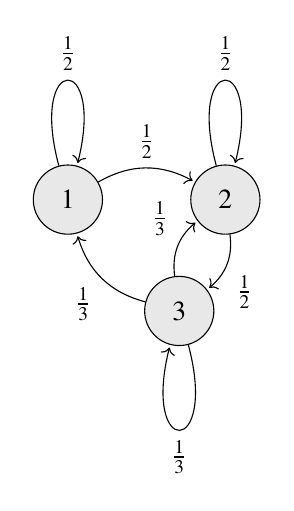
\begin{tikzpicture}[shorten >=1pt,node distance=2cm, scale =3, auto]
			\tikzstyle{every state}=[fill={rgb:black,1;white,10}]
			
			\node[state]   (q_1)                          {$1$};
			\node[state]   (q_2)  [right of=q_1]          {$2$};
			\node[state]   (q_3)  [below right of=q_1]          {$3$};
			
			\path[->]
			(q_1) edge [loop above] node {$\frac{1}{2}$}    (   )
			edge [bend left]  node {$\frac{1}{2}$}    (q_2)
			(q_2) edge [bend left]  node {$\frac{1}{2}$}    (q_3)
			edge [loop above] node {$\frac{1}{2}$}    ()
			(q_3) edge [bend left]  node {$\frac{1}{3}$}    (q_2)
			edge [bend left]  node {$\frac{1}{3}$}    (q_1)
			edge [loop below] node {$\frac{1}{3}$}    ();
		\end{tikzpicture}$
		
		\\  
		&\\
		&\\
		\hline
		\multirow{3}{*}{Checking whether the  } & \\
		& Here,\\chain is Irreducible
		& All the states are accessible to one another. \\and Aperiodic
		& $\implies$ They are in the same communication class. So, it is Irreducible.\\
		& \\
		& There exists the non- zero self-transition, which means that the chain \\
		& is Aperiodic.\\
		&\\ 
		& We know that if the Markov Chain is irreducible and aperiodic then \\
		& \qquad \qquad \qquad $\Vec{\pi}_{j} = \lim_{n \to \infty}P\{X_{n} = j\}$, $j = 1,...,N$ \\
		& These are the stationary probabilities. \\
		&\\
		\hline
		\multirow{3}{*}{Finding the Stationary} & \\
		& Stationary Probability can be represented as\\Probability Distributions
		& \qquad \qquad \qquad $\Vec{\pi} = \Vec{\pi} \vec{P}$\\
		& \\
		& \qquad $\implies$ $\myvec{v_{1}&&v_{2}&&v_{3}} = \myvec{v_{1}&&v_{2}&&v_{3}}\vec{P}$ \\
		& \\
		& Equating the above equation we get \\
		& \\
		& \qquad \qquad \qquad $\frac{1}{2}v_{1}-\frac{1}{3}v_{3} = 0$ $\label{eq:solutions/2018/dec/106/eq}$\\
		& \\
		& \qquad \qquad \qquad $\frac{1}{2}v_{1}-\frac{1}{2}v_{2} + \frac{1}{3}v_{3} = 0$\\
		& \\
		& \qquad \qquad \qquad $\frac{1}{2}v_{2}-\frac{2}{3}v_{3} = 0$\\
		& \\\
		& We see that summation of second and the third equation gives us the \\
		& first equation only. \\
		& And we know that the probability distribution will sum up to 1. \\
		& \\
		& \qquad \qquad \qquad $v_{1}+v_{2}+v_{3} = 1$ \\
		& \\
		& Therefore, we get the equation form as \\
		& \\
		& \qquad \qquad \qquad $\myvec{1&1&1\\\frac{1}{2}&0&\frac{-1}{3}\\\frac{1}{2}&\frac{-1}{2}&\frac{1}{3}}\myvec{v_{1}\\v_{2}\\v_{3}} = \myvec{1\\0\\0}$ \\
		& \\
		\hline
		\multirow{3}{*}{Solving the linear} & \\
		& The above linear equation can be solved using Gauss-Jordan method as\\equtions
		& \\
		& \qquad \qquad \qquad $\myvec{1&1&1&\vrule&1\\\frac{1}{2}&0&\frac{-1}{3}&\vrule&0\\\frac{1}{2}&\frac{-1}{2}&\frac{1}{3}&\vrule&0}$\\
		& \\
		& \qquad $\xleftrightarrow[]{R_2 \leftarrow R_2 - \frac{1}{2}R_1}$
		$\myvec{1&1&1&\vrule&1\\0&\frac{-1}{2}&\frac{-5}{6}&\vrule&\frac{-1}{2}\\\frac{1}{2}&\frac{-1}{2}&\frac{1}{3}&\vrule&0}$\\
		&\\
		& \qquad $\xleftrightarrow[]{R_3 \leftarrow R_3 - \frac{1}{2}R_1}$
		$\myvec{1&1&1&\vrule&1\\0&\frac{-1}{2}&\frac{-5}{6}&\vrule&\frac{-1}{2}\\0&-1&\frac{-1}{6}&\vrule&\frac{-1}{2}}$\\
		&\\
		& \qquad $\xleftrightarrow[]{R_2 \leftarrow \frac{-1}{2}R_2}$
		$\myvec{1&1&1&\vrule&1\\0&1&\frac{5}{3}&\vrule&1\\0&-1&\frac{-1}{6}&\vrule&\frac{-1}{2}}$\\
		&\\
		& \qquad $\xleftrightarrow[]{R_3 \leftarrow R_3 + R_2}$
		$\myvec{1&1&1&\vrule&1\\0&1&\frac{5}{3}&\vrule&1\\0&0&\frac{3}{2}&\vrule&\frac{1}{2}}$\\
		&\\
		& \qquad $\xleftrightarrow[]{R_3 \leftarrow \frac{3}{2}R_3}$
		$\myvec{1&1&1&\vrule&1\\0&1&\frac{5}{3}&\vrule&1\\0&0&1&\vrule&\frac{1}{3}}$\\
		&\\
		& \qquad $\xleftrightarrow[]{R_2 \leftarrow R_2 - \frac{5}{3}R_3}$
		$\myvec{1&1&1&\vrule&1\\0&1&0&\vrule&\frac{4}{9}\\0&0&1&\vrule&\frac{1}{3}}$\\
		&\\
		& \qquad $\xleftrightarrow[]{R_1 \leftarrow R_1 - R_3}$
		$\myvec{1&1&0&\vrule&\frac{2}{3}\\0&1&0&\vrule&\frac{4}{9}\\0&0&1&\vrule&\frac{1}{3}}$\\
		&\\
		& \qquad $\xleftrightarrow[]{R_1 \leftarrow R_1 - R_2}$
		$\myvec{1&0&0&\vrule&\frac{2}{9}\\0&1&0&\vrule&\frac{4}{9}\\0&0&1&\vrule&\frac{1}{3}}$\\
		&\\
		& $\therefore$, stationary probability distribution $\pi$ is given by \\
		& \qquad \qquad $\pi = \myvec{\frac{2}{9} & \frac{4}{9} & \frac{1}{3}}$ \\
		& \\
		\hline
		\multirow{3}{*}{Observations} & \\
		
		
		& Since the given transition probability matrix $\vec{P}$ is irreducible and aperiodic, \\
		& then $\lim_{n \to \infty} \vec{P}^{n}$ converges to a matrix with all rows identical and equal to $\vec{\pi}$. \\
		& \\
		& We were able to find $\vec{\pi}$ as $\myvec{\frac{2}{9} & \frac{4}{9} & \frac{1}{3}}$ \\
		& \\
		& $\lim_{n \to \infty} \vec{P}^{n} = \myvec{\frac{2}{9}&\frac{4}{9}&\frac{1}{3}\\\frac{2}{9}&\frac{4}{9}&\frac{1}{3}\\\frac{2}{9}&\frac{4}{9}&\frac{1}{3}}$\\
		& \\
		& From the above matrix, we get \\
		& \\
		& $\lim_{n \to \infty} \vec{P}^{n}_{11} = \frac{2}{9}$ \\
		&\\
		& $\lim_{n \to \infty} \vec{P}^{n}_{21} = \frac{2}{9}$ \\
		&\\
		& $\lim_{n \to \infty} \vec{P}^{n}_{32} = \frac{4}{9}$ \\
		&\\
		& $\lim_{n \to \infty} \vec{P}^{n}_{13} = \frac{1}{3}$ \\
		&\\
		\hline
		\multirow{3}{*}{Conclusion} & \\
		& From our observation we see that \\
		&\\
		& Options 1) and 4) are True.\\
		& \\
		\hline
\caption{}
\label{eq:solutions/2018/dec/106/table1}
	\end{longtable}
\twocolumn

\item Let
\begin{align}
\vec{A}=\myvec{1&0&2\\1&-2&0\\0&0&-3}
\end{align}
and $\vec{I}$ be the $3\times3$ identity matrix. If 
\begin{align}
6\vec{A}^{-1}=a\vec{A}^2+b\vec{A}+c\vec{I} \label{eq:solutions/2017/june/31/eq:1}
\end{align} for $a,b,c \in \mathbb{R}$ then (a,b,c) equals
\begin{enumerate}
\item (1,2,1)\\
\item (1,-1,2)\\
\item (4,1,1)\\
\item (1,4,1)
\end{enumerate}
\solution
See Tables \ref{eq:solutions/2018/dec/106/table0} and \ref{eq:solutions/2018/dec/106/table1}


\onecolumn
	\begin{longtable}{|l|l|}
		\hline
		\multirow{3}{*}{Irreducible Markov Chain} 
		& \\
		& A Markov chain is $\textbf{irreducible}$ if all the states communicate with each other,\\
		& i.e., if there is only one communication class.\\
		&\\
		\hline
		\multirow{3}{*}{Aperiodic Markov Chain} & \\
		& If there is a self-transition in the chain ($p^{ii}>0$ for some i), then the chain is\\
		& called as $\textbf{aperiodic}$\\
		& \\
		\hline
		\multirow{3}{*}{Stationary Distribution} & \\
		& A stationary distribution of a Markov chain is a probability distribution that\\
		& remains unchanged in the Markov chain as time progresses. Typically, it is\\
		& represented as a row vector $\Vec{\pi}$ whose entries are probabilities summing to 1,\\ 
		& and given transition matrix $\textbf{P}$, it satisfies\\
		& \\
		&  \qquad \qquad  \qquad$\Vec{\pi} = \Vec{\pi} \textbf{P}$\\
		& \\
		\hline
\caption{}
\label{eq:solutions/2018/dec/106/table0}
	\end{longtable}
	\begin{longtable}{|l|l|}
		\hline
		\multirow{3}{*}{Drawing Transition diagram} 
		& \\
		& 
		
		$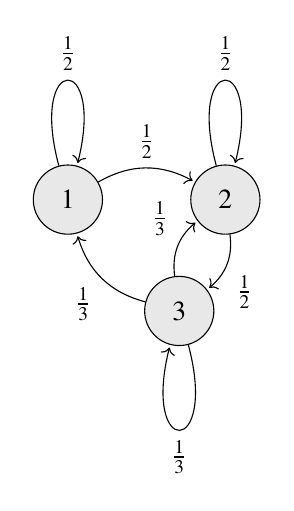
\begin{tikzpicture}[shorten >=1pt,node distance=2cm, scale =3, auto]
			\tikzstyle{every state}=[fill={rgb:black,1;white,10}]
			
			\node[state]   (q_1)                          {$1$};
			\node[state]   (q_2)  [right of=q_1]          {$2$};
			\node[state]   (q_3)  [below right of=q_1]          {$3$};
			
			\path[->]
			(q_1) edge [loop above] node {$\frac{1}{2}$}    (   )
			edge [bend left]  node {$\frac{1}{2}$}    (q_2)
			(q_2) edge [bend left]  node {$\frac{1}{2}$}    (q_3)
			edge [loop above] node {$\frac{1}{2}$}    ()
			(q_3) edge [bend left]  node {$\frac{1}{3}$}    (q_2)
			edge [bend left]  node {$\frac{1}{3}$}    (q_1)
			edge [loop below] node {$\frac{1}{3}$}    ();
		\end{tikzpicture}$
		
		\\  
		&\\
		&\\
		\hline
		\multirow{3}{*}{Checking whether the  } & \\
		& Here,\\chain is Irreducible
		& All the states are accessible to one another. \\and Aperiodic
		& $\implies$ They are in the same communication class. So, it is Irreducible.\\
		& \\
		& There exists the non- zero self-transition, which means that the chain \\
		& is Aperiodic.\\
		&\\ 
		& We know that if the Markov Chain is irreducible and aperiodic then \\
		& \qquad \qquad \qquad $\Vec{\pi}_{j} = \lim_{n \to \infty}P\{X_{n} = j\}$, $j = 1,...,N$ \\
		& These are the stationary probabilities. \\
		&\\
		\hline
		\multirow{3}{*}{Finding the Stationary} & \\
		& Stationary Probability can be represented as\\Probability Distributions
		& \qquad \qquad \qquad $\Vec{\pi} = \Vec{\pi} \vec{P}$\\
		& \\
		& \qquad $\implies$ $\myvec{v_{1}&&v_{2}&&v_{3}} = \myvec{v_{1}&&v_{2}&&v_{3}}\vec{P}$ \\
		& \\
		& Equating the above equation we get \\
		& \\
		& \qquad \qquad \qquad $\frac{1}{2}v_{1}-\frac{1}{3}v_{3} = 0$ $\label{eq:solutions/2018/dec/106/eq}$\\
		& \\
		& \qquad \qquad \qquad $\frac{1}{2}v_{1}-\frac{1}{2}v_{2} + \frac{1}{3}v_{3} = 0$\\
		& \\
		& \qquad \qquad \qquad $\frac{1}{2}v_{2}-\frac{2}{3}v_{3} = 0$\\
		& \\\
		& We see that summation of second and the third equation gives us the \\
		& first equation only. \\
		& And we know that the probability distribution will sum up to 1. \\
		& \\
		& \qquad \qquad \qquad $v_{1}+v_{2}+v_{3} = 1$ \\
		& \\
		& Therefore, we get the equation form as \\
		& \\
		& \qquad \qquad \qquad $\myvec{1&1&1\\\frac{1}{2}&0&\frac{-1}{3}\\\frac{1}{2}&\frac{-1}{2}&\frac{1}{3}}\myvec{v_{1}\\v_{2}\\v_{3}} = \myvec{1\\0\\0}$ \\
		& \\
		\hline
		\multirow{3}{*}{Solving the linear} & \\
		& The above linear equation can be solved using Gauss-Jordan method as\\equtions
		& \\
		& \qquad \qquad \qquad $\myvec{1&1&1&\vrule&1\\\frac{1}{2}&0&\frac{-1}{3}&\vrule&0\\\frac{1}{2}&\frac{-1}{2}&\frac{1}{3}&\vrule&0}$\\
		& \\
		& \qquad $\xleftrightarrow[]{R_2 \leftarrow R_2 - \frac{1}{2}R_1}$
		$\myvec{1&1&1&\vrule&1\\0&\frac{-1}{2}&\frac{-5}{6}&\vrule&\frac{-1}{2}\\\frac{1}{2}&\frac{-1}{2}&\frac{1}{3}&\vrule&0}$\\
		&\\
		& \qquad $\xleftrightarrow[]{R_3 \leftarrow R_3 - \frac{1}{2}R_1}$
		$\myvec{1&1&1&\vrule&1\\0&\frac{-1}{2}&\frac{-5}{6}&\vrule&\frac{-1}{2}\\0&-1&\frac{-1}{6}&\vrule&\frac{-1}{2}}$\\
		&\\
		& \qquad $\xleftrightarrow[]{R_2 \leftarrow \frac{-1}{2}R_2}$
		$\myvec{1&1&1&\vrule&1\\0&1&\frac{5}{3}&\vrule&1\\0&-1&\frac{-1}{6}&\vrule&\frac{-1}{2}}$\\
		&\\
		& \qquad $\xleftrightarrow[]{R_3 \leftarrow R_3 + R_2}$
		$\myvec{1&1&1&\vrule&1\\0&1&\frac{5}{3}&\vrule&1\\0&0&\frac{3}{2}&\vrule&\frac{1}{2}}$\\
		&\\
		& \qquad $\xleftrightarrow[]{R_3 \leftarrow \frac{3}{2}R_3}$
		$\myvec{1&1&1&\vrule&1\\0&1&\frac{5}{3}&\vrule&1\\0&0&1&\vrule&\frac{1}{3}}$\\
		&\\
		& \qquad $\xleftrightarrow[]{R_2 \leftarrow R_2 - \frac{5}{3}R_3}$
		$\myvec{1&1&1&\vrule&1\\0&1&0&\vrule&\frac{4}{9}\\0&0&1&\vrule&\frac{1}{3}}$\\
		&\\
		& \qquad $\xleftrightarrow[]{R_1 \leftarrow R_1 - R_3}$
		$\myvec{1&1&0&\vrule&\frac{2}{3}\\0&1&0&\vrule&\frac{4}{9}\\0&0&1&\vrule&\frac{1}{3}}$\\
		&\\
		& \qquad $\xleftrightarrow[]{R_1 \leftarrow R_1 - R_2}$
		$\myvec{1&0&0&\vrule&\frac{2}{9}\\0&1&0&\vrule&\frac{4}{9}\\0&0&1&\vrule&\frac{1}{3}}$\\
		&\\
		& $\therefore$, stationary probability distribution $\pi$ is given by \\
		& \qquad \qquad $\pi = \myvec{\frac{2}{9} & \frac{4}{9} & \frac{1}{3}}$ \\
		& \\
		\hline
		\multirow{3}{*}{Observations} & \\
		
		
		& Since the given transition probability matrix $\vec{P}$ is irreducible and aperiodic, \\
		& then $\lim_{n \to \infty} \vec{P}^{n}$ converges to a matrix with all rows identical and equal to $\vec{\pi}$. \\
		& \\
		& We were able to find $\vec{\pi}$ as $\myvec{\frac{2}{9} & \frac{4}{9} & \frac{1}{3}}$ \\
		& \\
		& $\lim_{n \to \infty} \vec{P}^{n} = \myvec{\frac{2}{9}&\frac{4}{9}&\frac{1}{3}\\\frac{2}{9}&\frac{4}{9}&\frac{1}{3}\\\frac{2}{9}&\frac{4}{9}&\frac{1}{3}}$\\
		& \\
		& From the above matrix, we get \\
		& \\
		& $\lim_{n \to \infty} \vec{P}^{n}_{11} = \frac{2}{9}$ \\
		&\\
		& $\lim_{n \to \infty} \vec{P}^{n}_{21} = \frac{2}{9}$ \\
		&\\
		& $\lim_{n \to \infty} \vec{P}^{n}_{32} = \frac{4}{9}$ \\
		&\\
		& $\lim_{n \to \infty} \vec{P}^{n}_{13} = \frac{1}{3}$ \\
		&\\
		\hline
		\multirow{3}{*}{Conclusion} & \\
		& From our observation we see that \\
		&\\
		& Options 1) and 4) are True.\\
		& \\
		\hline
\caption{}
\label{eq:solutions/2018/dec/106/table1}
	\end{longtable}
\twocolumn


%
\item Find the Eigenvalues of the matrix,
\begin{align}
\vec{A} = \myvec{1 & 1 & 2 \\ 1 & -2 & 5 \\ 2 & 5 & -3 }\label{eq:solutions/2017/june/32/eq:1}
\end{align}
\begin{enumerate}
\item -4, 3, -3
\item 4, 3, 1
\item 4, -4$\pm\sqrt{13}$
\item 4, -2$\pm\sqrt{7}$
\end{enumerate}
%
%
\solution
See Tables \ref{eq:solutions/2018/dec/106/table0} and \ref{eq:solutions/2018/dec/106/table1}


\onecolumn
	\begin{longtable}{|l|l|}
		\hline
		\multirow{3}{*}{Irreducible Markov Chain} 
		& \\
		& A Markov chain is $\textbf{irreducible}$ if all the states communicate with each other,\\
		& i.e., if there is only one communication class.\\
		&\\
		\hline
		\multirow{3}{*}{Aperiodic Markov Chain} & \\
		& If there is a self-transition in the chain ($p^{ii}>0$ for some i), then the chain is\\
		& called as $\textbf{aperiodic}$\\
		& \\
		\hline
		\multirow{3}{*}{Stationary Distribution} & \\
		& A stationary distribution of a Markov chain is a probability distribution that\\
		& remains unchanged in the Markov chain as time progresses. Typically, it is\\
		& represented as a row vector $\Vec{\pi}$ whose entries are probabilities summing to 1,\\ 
		& and given transition matrix $\textbf{P}$, it satisfies\\
		& \\
		&  \qquad \qquad  \qquad$\Vec{\pi} = \Vec{\pi} \textbf{P}$\\
		& \\
		\hline
\caption{}
\label{eq:solutions/2018/dec/106/table0}
	\end{longtable}
	\begin{longtable}{|l|l|}
		\hline
		\multirow{3}{*}{Drawing Transition diagram} 
		& \\
		& 
		
		$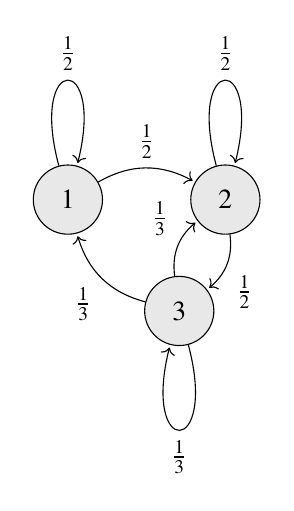
\begin{tikzpicture}[shorten >=1pt,node distance=2cm, scale =3, auto]
			\tikzstyle{every state}=[fill={rgb:black,1;white,10}]
			
			\node[state]   (q_1)                          {$1$};
			\node[state]   (q_2)  [right of=q_1]          {$2$};
			\node[state]   (q_3)  [below right of=q_1]          {$3$};
			
			\path[->]
			(q_1) edge [loop above] node {$\frac{1}{2}$}    (   )
			edge [bend left]  node {$\frac{1}{2}$}    (q_2)
			(q_2) edge [bend left]  node {$\frac{1}{2}$}    (q_3)
			edge [loop above] node {$\frac{1}{2}$}    ()
			(q_3) edge [bend left]  node {$\frac{1}{3}$}    (q_2)
			edge [bend left]  node {$\frac{1}{3}$}    (q_1)
			edge [loop below] node {$\frac{1}{3}$}    ();
		\end{tikzpicture}$
		
		\\  
		&\\
		&\\
		\hline
		\multirow{3}{*}{Checking whether the  } & \\
		& Here,\\chain is Irreducible
		& All the states are accessible to one another. \\and Aperiodic
		& $\implies$ They are in the same communication class. So, it is Irreducible.\\
		& \\
		& There exists the non- zero self-transition, which means that the chain \\
		& is Aperiodic.\\
		&\\ 
		& We know that if the Markov Chain is irreducible and aperiodic then \\
		& \qquad \qquad \qquad $\Vec{\pi}_{j} = \lim_{n \to \infty}P\{X_{n} = j\}$, $j = 1,...,N$ \\
		& These are the stationary probabilities. \\
		&\\
		\hline
		\multirow{3}{*}{Finding the Stationary} & \\
		& Stationary Probability can be represented as\\Probability Distributions
		& \qquad \qquad \qquad $\Vec{\pi} = \Vec{\pi} \vec{P}$\\
		& \\
		& \qquad $\implies$ $\myvec{v_{1}&&v_{2}&&v_{3}} = \myvec{v_{1}&&v_{2}&&v_{3}}\vec{P}$ \\
		& \\
		& Equating the above equation we get \\
		& \\
		& \qquad \qquad \qquad $\frac{1}{2}v_{1}-\frac{1}{3}v_{3} = 0$ $\label{eq:solutions/2018/dec/106/eq}$\\
		& \\
		& \qquad \qquad \qquad $\frac{1}{2}v_{1}-\frac{1}{2}v_{2} + \frac{1}{3}v_{3} = 0$\\
		& \\
		& \qquad \qquad \qquad $\frac{1}{2}v_{2}-\frac{2}{3}v_{3} = 0$\\
		& \\\
		& We see that summation of second and the third equation gives us the \\
		& first equation only. \\
		& And we know that the probability distribution will sum up to 1. \\
		& \\
		& \qquad \qquad \qquad $v_{1}+v_{2}+v_{3} = 1$ \\
		& \\
		& Therefore, we get the equation form as \\
		& \\
		& \qquad \qquad \qquad $\myvec{1&1&1\\\frac{1}{2}&0&\frac{-1}{3}\\\frac{1}{2}&\frac{-1}{2}&\frac{1}{3}}\myvec{v_{1}\\v_{2}\\v_{3}} = \myvec{1\\0\\0}$ \\
		& \\
		\hline
		\multirow{3}{*}{Solving the linear} & \\
		& The above linear equation can be solved using Gauss-Jordan method as\\equtions
		& \\
		& \qquad \qquad \qquad $\myvec{1&1&1&\vrule&1\\\frac{1}{2}&0&\frac{-1}{3}&\vrule&0\\\frac{1}{2}&\frac{-1}{2}&\frac{1}{3}&\vrule&0}$\\
		& \\
		& \qquad $\xleftrightarrow[]{R_2 \leftarrow R_2 - \frac{1}{2}R_1}$
		$\myvec{1&1&1&\vrule&1\\0&\frac{-1}{2}&\frac{-5}{6}&\vrule&\frac{-1}{2}\\\frac{1}{2}&\frac{-1}{2}&\frac{1}{3}&\vrule&0}$\\
		&\\
		& \qquad $\xleftrightarrow[]{R_3 \leftarrow R_3 - \frac{1}{2}R_1}$
		$\myvec{1&1&1&\vrule&1\\0&\frac{-1}{2}&\frac{-5}{6}&\vrule&\frac{-1}{2}\\0&-1&\frac{-1}{6}&\vrule&\frac{-1}{2}}$\\
		&\\
		& \qquad $\xleftrightarrow[]{R_2 \leftarrow \frac{-1}{2}R_2}$
		$\myvec{1&1&1&\vrule&1\\0&1&\frac{5}{3}&\vrule&1\\0&-1&\frac{-1}{6}&\vrule&\frac{-1}{2}}$\\
		&\\
		& \qquad $\xleftrightarrow[]{R_3 \leftarrow R_3 + R_2}$
		$\myvec{1&1&1&\vrule&1\\0&1&\frac{5}{3}&\vrule&1\\0&0&\frac{3}{2}&\vrule&\frac{1}{2}}$\\
		&\\
		& \qquad $\xleftrightarrow[]{R_3 \leftarrow \frac{3}{2}R_3}$
		$\myvec{1&1&1&\vrule&1\\0&1&\frac{5}{3}&\vrule&1\\0&0&1&\vrule&\frac{1}{3}}$\\
		&\\
		& \qquad $\xleftrightarrow[]{R_2 \leftarrow R_2 - \frac{5}{3}R_3}$
		$\myvec{1&1&1&\vrule&1\\0&1&0&\vrule&\frac{4}{9}\\0&0&1&\vrule&\frac{1}{3}}$\\
		&\\
		& \qquad $\xleftrightarrow[]{R_1 \leftarrow R_1 - R_3}$
		$\myvec{1&1&0&\vrule&\frac{2}{3}\\0&1&0&\vrule&\frac{4}{9}\\0&0&1&\vrule&\frac{1}{3}}$\\
		&\\
		& \qquad $\xleftrightarrow[]{R_1 \leftarrow R_1 - R_2}$
		$\myvec{1&0&0&\vrule&\frac{2}{9}\\0&1&0&\vrule&\frac{4}{9}\\0&0&1&\vrule&\frac{1}{3}}$\\
		&\\
		& $\therefore$, stationary probability distribution $\pi$ is given by \\
		& \qquad \qquad $\pi = \myvec{\frac{2}{9} & \frac{4}{9} & \frac{1}{3}}$ \\
		& \\
		\hline
		\multirow{3}{*}{Observations} & \\
		
		
		& Since the given transition probability matrix $\vec{P}$ is irreducible and aperiodic, \\
		& then $\lim_{n \to \infty} \vec{P}^{n}$ converges to a matrix with all rows identical and equal to $\vec{\pi}$. \\
		& \\
		& We were able to find $\vec{\pi}$ as $\myvec{\frac{2}{9} & \frac{4}{9} & \frac{1}{3}}$ \\
		& \\
		& $\lim_{n \to \infty} \vec{P}^{n} = \myvec{\frac{2}{9}&\frac{4}{9}&\frac{1}{3}\\\frac{2}{9}&\frac{4}{9}&\frac{1}{3}\\\frac{2}{9}&\frac{4}{9}&\frac{1}{3}}$\\
		& \\
		& From the above matrix, we get \\
		& \\
		& $\lim_{n \to \infty} \vec{P}^{n}_{11} = \frac{2}{9}$ \\
		&\\
		& $\lim_{n \to \infty} \vec{P}^{n}_{21} = \frac{2}{9}$ \\
		&\\
		& $\lim_{n \to \infty} \vec{P}^{n}_{32} = \frac{4}{9}$ \\
		&\\
		& $\lim_{n \to \infty} \vec{P}^{n}_{13} = \frac{1}{3}$ \\
		&\\
		\hline
		\multirow{3}{*}{Conclusion} & \\
		& From our observation we see that \\
		&\\
		& Options 1) and 4) are True.\\
		& \\
		\hline
\caption{}
\label{eq:solutions/2018/dec/106/table1}
	\end{longtable}
\twocolumn

\item Consider the vector space V of real polynomials of degree less than or equal to n. Fix distinct real numbers $a_0, a_1, \cdots, a_k$. For $p \in V$
\begin{align}
    max\cbrak{\abs{p(a_j)}: 0\leq j \leq k}
\end{align}
defines a norm on V
\begin{enumerate}
    \item only if $k<n$
    \item only if $k\ge n$
    \item if $ k+1\leq n$ 
    \item if $k \ge n+1$
\end{enumerate}
%
\solution
See Tables \ref{eq:solutions/2018/dec/106/table0} and \ref{eq:solutions/2018/dec/106/table1}


\onecolumn
	\begin{longtable}{|l|l|}
		\hline
		\multirow{3}{*}{Irreducible Markov Chain} 
		& \\
		& A Markov chain is $\textbf{irreducible}$ if all the states communicate with each other,\\
		& i.e., if there is only one communication class.\\
		&\\
		\hline
		\multirow{3}{*}{Aperiodic Markov Chain} & \\
		& If there is a self-transition in the chain ($p^{ii}>0$ for some i), then the chain is\\
		& called as $\textbf{aperiodic}$\\
		& \\
		\hline
		\multirow{3}{*}{Stationary Distribution} & \\
		& A stationary distribution of a Markov chain is a probability distribution that\\
		& remains unchanged in the Markov chain as time progresses. Typically, it is\\
		& represented as a row vector $\Vec{\pi}$ whose entries are probabilities summing to 1,\\ 
		& and given transition matrix $\textbf{P}$, it satisfies\\
		& \\
		&  \qquad \qquad  \qquad$\Vec{\pi} = \Vec{\pi} \textbf{P}$\\
		& \\
		\hline
\caption{}
\label{eq:solutions/2018/dec/106/table0}
	\end{longtable}
	\begin{longtable}{|l|l|}
		\hline
		\multirow{3}{*}{Drawing Transition diagram} 
		& \\
		& 
		
		$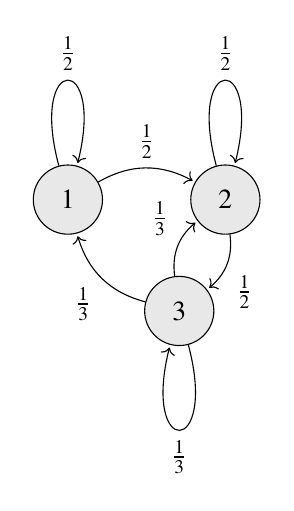
\begin{tikzpicture}[shorten >=1pt,node distance=2cm, scale =3, auto]
			\tikzstyle{every state}=[fill={rgb:black,1;white,10}]
			
			\node[state]   (q_1)                          {$1$};
			\node[state]   (q_2)  [right of=q_1]          {$2$};
			\node[state]   (q_3)  [below right of=q_1]          {$3$};
			
			\path[->]
			(q_1) edge [loop above] node {$\frac{1}{2}$}    (   )
			edge [bend left]  node {$\frac{1}{2}$}    (q_2)
			(q_2) edge [bend left]  node {$\frac{1}{2}$}    (q_3)
			edge [loop above] node {$\frac{1}{2}$}    ()
			(q_3) edge [bend left]  node {$\frac{1}{3}$}    (q_2)
			edge [bend left]  node {$\frac{1}{3}$}    (q_1)
			edge [loop below] node {$\frac{1}{3}$}    ();
		\end{tikzpicture}$
		
		\\  
		&\\
		&\\
		\hline
		\multirow{3}{*}{Checking whether the  } & \\
		& Here,\\chain is Irreducible
		& All the states are accessible to one another. \\and Aperiodic
		& $\implies$ They are in the same communication class. So, it is Irreducible.\\
		& \\
		& There exists the non- zero self-transition, which means that the chain \\
		& is Aperiodic.\\
		&\\ 
		& We know that if the Markov Chain is irreducible and aperiodic then \\
		& \qquad \qquad \qquad $\Vec{\pi}_{j} = \lim_{n \to \infty}P\{X_{n} = j\}$, $j = 1,...,N$ \\
		& These are the stationary probabilities. \\
		&\\
		\hline
		\multirow{3}{*}{Finding the Stationary} & \\
		& Stationary Probability can be represented as\\Probability Distributions
		& \qquad \qquad \qquad $\Vec{\pi} = \Vec{\pi} \vec{P}$\\
		& \\
		& \qquad $\implies$ $\myvec{v_{1}&&v_{2}&&v_{3}} = \myvec{v_{1}&&v_{2}&&v_{3}}\vec{P}$ \\
		& \\
		& Equating the above equation we get \\
		& \\
		& \qquad \qquad \qquad $\frac{1}{2}v_{1}-\frac{1}{3}v_{3} = 0$ $\label{eq:solutions/2018/dec/106/eq}$\\
		& \\
		& \qquad \qquad \qquad $\frac{1}{2}v_{1}-\frac{1}{2}v_{2} + \frac{1}{3}v_{3} = 0$\\
		& \\
		& \qquad \qquad \qquad $\frac{1}{2}v_{2}-\frac{2}{3}v_{3} = 0$\\
		& \\\
		& We see that summation of second and the third equation gives us the \\
		& first equation only. \\
		& And we know that the probability distribution will sum up to 1. \\
		& \\
		& \qquad \qquad \qquad $v_{1}+v_{2}+v_{3} = 1$ \\
		& \\
		& Therefore, we get the equation form as \\
		& \\
		& \qquad \qquad \qquad $\myvec{1&1&1\\\frac{1}{2}&0&\frac{-1}{3}\\\frac{1}{2}&\frac{-1}{2}&\frac{1}{3}}\myvec{v_{1}\\v_{2}\\v_{3}} = \myvec{1\\0\\0}$ \\
		& \\
		\hline
		\multirow{3}{*}{Solving the linear} & \\
		& The above linear equation can be solved using Gauss-Jordan method as\\equtions
		& \\
		& \qquad \qquad \qquad $\myvec{1&1&1&\vrule&1\\\frac{1}{2}&0&\frac{-1}{3}&\vrule&0\\\frac{1}{2}&\frac{-1}{2}&\frac{1}{3}&\vrule&0}$\\
		& \\
		& \qquad $\xleftrightarrow[]{R_2 \leftarrow R_2 - \frac{1}{2}R_1}$
		$\myvec{1&1&1&\vrule&1\\0&\frac{-1}{2}&\frac{-5}{6}&\vrule&\frac{-1}{2}\\\frac{1}{2}&\frac{-1}{2}&\frac{1}{3}&\vrule&0}$\\
		&\\
		& \qquad $\xleftrightarrow[]{R_3 \leftarrow R_3 - \frac{1}{2}R_1}$
		$\myvec{1&1&1&\vrule&1\\0&\frac{-1}{2}&\frac{-5}{6}&\vrule&\frac{-1}{2}\\0&-1&\frac{-1}{6}&\vrule&\frac{-1}{2}}$\\
		&\\
		& \qquad $\xleftrightarrow[]{R_2 \leftarrow \frac{-1}{2}R_2}$
		$\myvec{1&1&1&\vrule&1\\0&1&\frac{5}{3}&\vrule&1\\0&-1&\frac{-1}{6}&\vrule&\frac{-1}{2}}$\\
		&\\
		& \qquad $\xleftrightarrow[]{R_3 \leftarrow R_3 + R_2}$
		$\myvec{1&1&1&\vrule&1\\0&1&\frac{5}{3}&\vrule&1\\0&0&\frac{3}{2}&\vrule&\frac{1}{2}}$\\
		&\\
		& \qquad $\xleftrightarrow[]{R_3 \leftarrow \frac{3}{2}R_3}$
		$\myvec{1&1&1&\vrule&1\\0&1&\frac{5}{3}&\vrule&1\\0&0&1&\vrule&\frac{1}{3}}$\\
		&\\
		& \qquad $\xleftrightarrow[]{R_2 \leftarrow R_2 - \frac{5}{3}R_3}$
		$\myvec{1&1&1&\vrule&1\\0&1&0&\vrule&\frac{4}{9}\\0&0&1&\vrule&\frac{1}{3}}$\\
		&\\
		& \qquad $\xleftrightarrow[]{R_1 \leftarrow R_1 - R_3}$
		$\myvec{1&1&0&\vrule&\frac{2}{3}\\0&1&0&\vrule&\frac{4}{9}\\0&0&1&\vrule&\frac{1}{3}}$\\
		&\\
		& \qquad $\xleftrightarrow[]{R_1 \leftarrow R_1 - R_2}$
		$\myvec{1&0&0&\vrule&\frac{2}{9}\\0&1&0&\vrule&\frac{4}{9}\\0&0&1&\vrule&\frac{1}{3}}$\\
		&\\
		& $\therefore$, stationary probability distribution $\pi$ is given by \\
		& \qquad \qquad $\pi = \myvec{\frac{2}{9} & \frac{4}{9} & \frac{1}{3}}$ \\
		& \\
		\hline
		\multirow{3}{*}{Observations} & \\
		
		
		& Since the given transition probability matrix $\vec{P}$ is irreducible and aperiodic, \\
		& then $\lim_{n \to \infty} \vec{P}^{n}$ converges to a matrix with all rows identical and equal to $\vec{\pi}$. \\
		& \\
		& We were able to find $\vec{\pi}$ as $\myvec{\frac{2}{9} & \frac{4}{9} & \frac{1}{3}}$ \\
		& \\
		& $\lim_{n \to \infty} \vec{P}^{n} = \myvec{\frac{2}{9}&\frac{4}{9}&\frac{1}{3}\\\frac{2}{9}&\frac{4}{9}&\frac{1}{3}\\\frac{2}{9}&\frac{4}{9}&\frac{1}{3}}$\\
		& \\
		& From the above matrix, we get \\
		& \\
		& $\lim_{n \to \infty} \vec{P}^{n}_{11} = \frac{2}{9}$ \\
		&\\
		& $\lim_{n \to \infty} \vec{P}^{n}_{21} = \frac{2}{9}$ \\
		&\\
		& $\lim_{n \to \infty} \vec{P}^{n}_{32} = \frac{4}{9}$ \\
		&\\
		& $\lim_{n \to \infty} \vec{P}^{n}_{13} = \frac{1}{3}$ \\
		&\\
		\hline
		\multirow{3}{*}{Conclusion} & \\
		& From our observation we see that \\
		&\\
		& Options 1) and 4) are True.\\
		& \\
		\hline
\caption{}
\label{eq:solutions/2018/dec/106/table1}
	\end{longtable}
\twocolumn

\item Let \textbf{V} be the vector space of polynomials of degree at most 3 in a variable x with coefficients in $\mathbb{R}$. Let \textbf{T}=d/dx be the linear transformation of \textbf{V} to itself given by differentiation.\\

Which of the following are correct?\\
\begin{enumerate}
\item $\vec{T}$ is invertible
\item 0 is an eigenvalue of $\vec{T}$
\item There is a basis with respect to which the matrix of \textbf{T} is nilpotent.
\item The matrix of \textbf{T} with respect to the basis \myvec{1,1+x,1+x+x^2,1+x+x^2+x^3} is diagonal.
\end{enumerate}
\solution
See Tables \ref{eq:solutions/2018/dec/106/table0} and \ref{eq:solutions/2018/dec/106/table1}


\onecolumn
	\begin{longtable}{|l|l|}
		\hline
		\multirow{3}{*}{Irreducible Markov Chain} 
		& \\
		& A Markov chain is $\textbf{irreducible}$ if all the states communicate with each other,\\
		& i.e., if there is only one communication class.\\
		&\\
		\hline
		\multirow{3}{*}{Aperiodic Markov Chain} & \\
		& If there is a self-transition in the chain ($p^{ii}>0$ for some i), then the chain is\\
		& called as $\textbf{aperiodic}$\\
		& \\
		\hline
		\multirow{3}{*}{Stationary Distribution} & \\
		& A stationary distribution of a Markov chain is a probability distribution that\\
		& remains unchanged in the Markov chain as time progresses. Typically, it is\\
		& represented as a row vector $\Vec{\pi}$ whose entries are probabilities summing to 1,\\ 
		& and given transition matrix $\textbf{P}$, it satisfies\\
		& \\
		&  \qquad \qquad  \qquad$\Vec{\pi} = \Vec{\pi} \textbf{P}$\\
		& \\
		\hline
\caption{}
\label{eq:solutions/2018/dec/106/table0}
	\end{longtable}
	\begin{longtable}{|l|l|}
		\hline
		\multirow{3}{*}{Drawing Transition diagram} 
		& \\
		& 
		
		$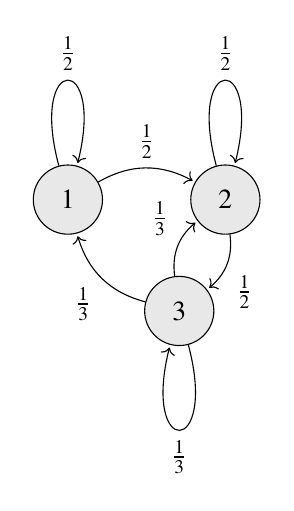
\begin{tikzpicture}[shorten >=1pt,node distance=2cm, scale =3, auto]
			\tikzstyle{every state}=[fill={rgb:black,1;white,10}]
			
			\node[state]   (q_1)                          {$1$};
			\node[state]   (q_2)  [right of=q_1]          {$2$};
			\node[state]   (q_3)  [below right of=q_1]          {$3$};
			
			\path[->]
			(q_1) edge [loop above] node {$\frac{1}{2}$}    (   )
			edge [bend left]  node {$\frac{1}{2}$}    (q_2)
			(q_2) edge [bend left]  node {$\frac{1}{2}$}    (q_3)
			edge [loop above] node {$\frac{1}{2}$}    ()
			(q_3) edge [bend left]  node {$\frac{1}{3}$}    (q_2)
			edge [bend left]  node {$\frac{1}{3}$}    (q_1)
			edge [loop below] node {$\frac{1}{3}$}    ();
		\end{tikzpicture}$
		
		\\  
		&\\
		&\\
		\hline
		\multirow{3}{*}{Checking whether the  } & \\
		& Here,\\chain is Irreducible
		& All the states are accessible to one another. \\and Aperiodic
		& $\implies$ They are in the same communication class. So, it is Irreducible.\\
		& \\
		& There exists the non- zero self-transition, which means that the chain \\
		& is Aperiodic.\\
		&\\ 
		& We know that if the Markov Chain is irreducible and aperiodic then \\
		& \qquad \qquad \qquad $\Vec{\pi}_{j} = \lim_{n \to \infty}P\{X_{n} = j\}$, $j = 1,...,N$ \\
		& These are the stationary probabilities. \\
		&\\
		\hline
		\multirow{3}{*}{Finding the Stationary} & \\
		& Stationary Probability can be represented as\\Probability Distributions
		& \qquad \qquad \qquad $\Vec{\pi} = \Vec{\pi} \vec{P}$\\
		& \\
		& \qquad $\implies$ $\myvec{v_{1}&&v_{2}&&v_{3}} = \myvec{v_{1}&&v_{2}&&v_{3}}\vec{P}$ \\
		& \\
		& Equating the above equation we get \\
		& \\
		& \qquad \qquad \qquad $\frac{1}{2}v_{1}-\frac{1}{3}v_{3} = 0$ $\label{eq:solutions/2018/dec/106/eq}$\\
		& \\
		& \qquad \qquad \qquad $\frac{1}{2}v_{1}-\frac{1}{2}v_{2} + \frac{1}{3}v_{3} = 0$\\
		& \\
		& \qquad \qquad \qquad $\frac{1}{2}v_{2}-\frac{2}{3}v_{3} = 0$\\
		& \\\
		& We see that summation of second and the third equation gives us the \\
		& first equation only. \\
		& And we know that the probability distribution will sum up to 1. \\
		& \\
		& \qquad \qquad \qquad $v_{1}+v_{2}+v_{3} = 1$ \\
		& \\
		& Therefore, we get the equation form as \\
		& \\
		& \qquad \qquad \qquad $\myvec{1&1&1\\\frac{1}{2}&0&\frac{-1}{3}\\\frac{1}{2}&\frac{-1}{2}&\frac{1}{3}}\myvec{v_{1}\\v_{2}\\v_{3}} = \myvec{1\\0\\0}$ \\
		& \\
		\hline
		\multirow{3}{*}{Solving the linear} & \\
		& The above linear equation can be solved using Gauss-Jordan method as\\equtions
		& \\
		& \qquad \qquad \qquad $\myvec{1&1&1&\vrule&1\\\frac{1}{2}&0&\frac{-1}{3}&\vrule&0\\\frac{1}{2}&\frac{-1}{2}&\frac{1}{3}&\vrule&0}$\\
		& \\
		& \qquad $\xleftrightarrow[]{R_2 \leftarrow R_2 - \frac{1}{2}R_1}$
		$\myvec{1&1&1&\vrule&1\\0&\frac{-1}{2}&\frac{-5}{6}&\vrule&\frac{-1}{2}\\\frac{1}{2}&\frac{-1}{2}&\frac{1}{3}&\vrule&0}$\\
		&\\
		& \qquad $\xleftrightarrow[]{R_3 \leftarrow R_3 - \frac{1}{2}R_1}$
		$\myvec{1&1&1&\vrule&1\\0&\frac{-1}{2}&\frac{-5}{6}&\vrule&\frac{-1}{2}\\0&-1&\frac{-1}{6}&\vrule&\frac{-1}{2}}$\\
		&\\
		& \qquad $\xleftrightarrow[]{R_2 \leftarrow \frac{-1}{2}R_2}$
		$\myvec{1&1&1&\vrule&1\\0&1&\frac{5}{3}&\vrule&1\\0&-1&\frac{-1}{6}&\vrule&\frac{-1}{2}}$\\
		&\\
		& \qquad $\xleftrightarrow[]{R_3 \leftarrow R_3 + R_2}$
		$\myvec{1&1&1&\vrule&1\\0&1&\frac{5}{3}&\vrule&1\\0&0&\frac{3}{2}&\vrule&\frac{1}{2}}$\\
		&\\
		& \qquad $\xleftrightarrow[]{R_3 \leftarrow \frac{3}{2}R_3}$
		$\myvec{1&1&1&\vrule&1\\0&1&\frac{5}{3}&\vrule&1\\0&0&1&\vrule&\frac{1}{3}}$\\
		&\\
		& \qquad $\xleftrightarrow[]{R_2 \leftarrow R_2 - \frac{5}{3}R_3}$
		$\myvec{1&1&1&\vrule&1\\0&1&0&\vrule&\frac{4}{9}\\0&0&1&\vrule&\frac{1}{3}}$\\
		&\\
		& \qquad $\xleftrightarrow[]{R_1 \leftarrow R_1 - R_3}$
		$\myvec{1&1&0&\vrule&\frac{2}{3}\\0&1&0&\vrule&\frac{4}{9}\\0&0&1&\vrule&\frac{1}{3}}$\\
		&\\
		& \qquad $\xleftrightarrow[]{R_1 \leftarrow R_1 - R_2}$
		$\myvec{1&0&0&\vrule&\frac{2}{9}\\0&1&0&\vrule&\frac{4}{9}\\0&0&1&\vrule&\frac{1}{3}}$\\
		&\\
		& $\therefore$, stationary probability distribution $\pi$ is given by \\
		& \qquad \qquad $\pi = \myvec{\frac{2}{9} & \frac{4}{9} & \frac{1}{3}}$ \\
		& \\
		\hline
		\multirow{3}{*}{Observations} & \\
		
		
		& Since the given transition probability matrix $\vec{P}$ is irreducible and aperiodic, \\
		& then $\lim_{n \to \infty} \vec{P}^{n}$ converges to a matrix with all rows identical and equal to $\vec{\pi}$. \\
		& \\
		& We were able to find $\vec{\pi}$ as $\myvec{\frac{2}{9} & \frac{4}{9} & \frac{1}{3}}$ \\
		& \\
		& $\lim_{n \to \infty} \vec{P}^{n} = \myvec{\frac{2}{9}&\frac{4}{9}&\frac{1}{3}\\\frac{2}{9}&\frac{4}{9}&\frac{1}{3}\\\frac{2}{9}&\frac{4}{9}&\frac{1}{3}}$\\
		& \\
		& From the above matrix, we get \\
		& \\
		& $\lim_{n \to \infty} \vec{P}^{n}_{11} = \frac{2}{9}$ \\
		&\\
		& $\lim_{n \to \infty} \vec{P}^{n}_{21} = \frac{2}{9}$ \\
		&\\
		& $\lim_{n \to \infty} \vec{P}^{n}_{32} = \frac{4}{9}$ \\
		&\\
		& $\lim_{n \to \infty} \vec{P}^{n}_{13} = \frac{1}{3}$ \\
		&\\
		\hline
		\multirow{3}{*}{Conclusion} & \\
		& From our observation we see that \\
		&\\
		& Options 1) and 4) are True.\\
		& \\
		\hline
\caption{}
\label{eq:solutions/2018/dec/106/table1}
	\end{longtable}
\twocolumn

\item Let $m,n,r$ be natural numbers. Let $A$ be an $m\times n$ matrix with real entries such that $(AA^t)^r = I$, where $I$ is the $m \times m$ is identity matrix and $A^t$ is the transpose of the matrix $A$. We can conclude that\\
\begin{enumerate}
\item
$m = n$\\
\item
$AA^t$ is invertible\\
\item
$A^tA$ is invertible\\
\item
if $m=n$, then $A$ is invertible
\end{enumerate}
%
\solution
See Tables \ref{eq:solutions/2018/dec/106/table0} and \ref{eq:solutions/2018/dec/106/table1}


\onecolumn
	\begin{longtable}{|l|l|}
		\hline
		\multirow{3}{*}{Irreducible Markov Chain} 
		& \\
		& A Markov chain is $\textbf{irreducible}$ if all the states communicate with each other,\\
		& i.e., if there is only one communication class.\\
		&\\
		\hline
		\multirow{3}{*}{Aperiodic Markov Chain} & \\
		& If there is a self-transition in the chain ($p^{ii}>0$ for some i), then the chain is\\
		& called as $\textbf{aperiodic}$\\
		& \\
		\hline
		\multirow{3}{*}{Stationary Distribution} & \\
		& A stationary distribution of a Markov chain is a probability distribution that\\
		& remains unchanged in the Markov chain as time progresses. Typically, it is\\
		& represented as a row vector $\Vec{\pi}$ whose entries are probabilities summing to 1,\\ 
		& and given transition matrix $\textbf{P}$, it satisfies\\
		& \\
		&  \qquad \qquad  \qquad$\Vec{\pi} = \Vec{\pi} \textbf{P}$\\
		& \\
		\hline
\caption{}
\label{eq:solutions/2018/dec/106/table0}
	\end{longtable}
	\begin{longtable}{|l|l|}
		\hline
		\multirow{3}{*}{Drawing Transition diagram} 
		& \\
		& 
		
		$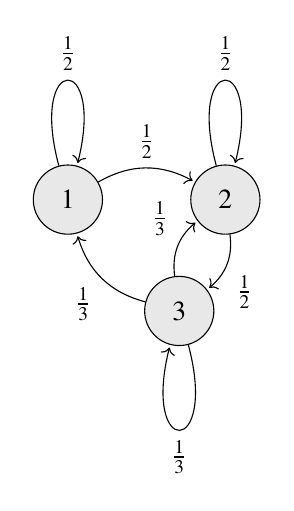
\begin{tikzpicture}[shorten >=1pt,node distance=2cm, scale =3, auto]
			\tikzstyle{every state}=[fill={rgb:black,1;white,10}]
			
			\node[state]   (q_1)                          {$1$};
			\node[state]   (q_2)  [right of=q_1]          {$2$};
			\node[state]   (q_3)  [below right of=q_1]          {$3$};
			
			\path[->]
			(q_1) edge [loop above] node {$\frac{1}{2}$}    (   )
			edge [bend left]  node {$\frac{1}{2}$}    (q_2)
			(q_2) edge [bend left]  node {$\frac{1}{2}$}    (q_3)
			edge [loop above] node {$\frac{1}{2}$}    ()
			(q_3) edge [bend left]  node {$\frac{1}{3}$}    (q_2)
			edge [bend left]  node {$\frac{1}{3}$}    (q_1)
			edge [loop below] node {$\frac{1}{3}$}    ();
		\end{tikzpicture}$
		
		\\  
		&\\
		&\\
		\hline
		\multirow{3}{*}{Checking whether the  } & \\
		& Here,\\chain is Irreducible
		& All the states are accessible to one another. \\and Aperiodic
		& $\implies$ They are in the same communication class. So, it is Irreducible.\\
		& \\
		& There exists the non- zero self-transition, which means that the chain \\
		& is Aperiodic.\\
		&\\ 
		& We know that if the Markov Chain is irreducible and aperiodic then \\
		& \qquad \qquad \qquad $\Vec{\pi}_{j} = \lim_{n \to \infty}P\{X_{n} = j\}$, $j = 1,...,N$ \\
		& These are the stationary probabilities. \\
		&\\
		\hline
		\multirow{3}{*}{Finding the Stationary} & \\
		& Stationary Probability can be represented as\\Probability Distributions
		& \qquad \qquad \qquad $\Vec{\pi} = \Vec{\pi} \vec{P}$\\
		& \\
		& \qquad $\implies$ $\myvec{v_{1}&&v_{2}&&v_{3}} = \myvec{v_{1}&&v_{2}&&v_{3}}\vec{P}$ \\
		& \\
		& Equating the above equation we get \\
		& \\
		& \qquad \qquad \qquad $\frac{1}{2}v_{1}-\frac{1}{3}v_{3} = 0$ $\label{eq:solutions/2018/dec/106/eq}$\\
		& \\
		& \qquad \qquad \qquad $\frac{1}{2}v_{1}-\frac{1}{2}v_{2} + \frac{1}{3}v_{3} = 0$\\
		& \\
		& \qquad \qquad \qquad $\frac{1}{2}v_{2}-\frac{2}{3}v_{3} = 0$\\
		& \\\
		& We see that summation of second and the third equation gives us the \\
		& first equation only. \\
		& And we know that the probability distribution will sum up to 1. \\
		& \\
		& \qquad \qquad \qquad $v_{1}+v_{2}+v_{3} = 1$ \\
		& \\
		& Therefore, we get the equation form as \\
		& \\
		& \qquad \qquad \qquad $\myvec{1&1&1\\\frac{1}{2}&0&\frac{-1}{3}\\\frac{1}{2}&\frac{-1}{2}&\frac{1}{3}}\myvec{v_{1}\\v_{2}\\v_{3}} = \myvec{1\\0\\0}$ \\
		& \\
		\hline
		\multirow{3}{*}{Solving the linear} & \\
		& The above linear equation can be solved using Gauss-Jordan method as\\equtions
		& \\
		& \qquad \qquad \qquad $\myvec{1&1&1&\vrule&1\\\frac{1}{2}&0&\frac{-1}{3}&\vrule&0\\\frac{1}{2}&\frac{-1}{2}&\frac{1}{3}&\vrule&0}$\\
		& \\
		& \qquad $\xleftrightarrow[]{R_2 \leftarrow R_2 - \frac{1}{2}R_1}$
		$\myvec{1&1&1&\vrule&1\\0&\frac{-1}{2}&\frac{-5}{6}&\vrule&\frac{-1}{2}\\\frac{1}{2}&\frac{-1}{2}&\frac{1}{3}&\vrule&0}$\\
		&\\
		& \qquad $\xleftrightarrow[]{R_3 \leftarrow R_3 - \frac{1}{2}R_1}$
		$\myvec{1&1&1&\vrule&1\\0&\frac{-1}{2}&\frac{-5}{6}&\vrule&\frac{-1}{2}\\0&-1&\frac{-1}{6}&\vrule&\frac{-1}{2}}$\\
		&\\
		& \qquad $\xleftrightarrow[]{R_2 \leftarrow \frac{-1}{2}R_2}$
		$\myvec{1&1&1&\vrule&1\\0&1&\frac{5}{3}&\vrule&1\\0&-1&\frac{-1}{6}&\vrule&\frac{-1}{2}}$\\
		&\\
		& \qquad $\xleftrightarrow[]{R_3 \leftarrow R_3 + R_2}$
		$\myvec{1&1&1&\vrule&1\\0&1&\frac{5}{3}&\vrule&1\\0&0&\frac{3}{2}&\vrule&\frac{1}{2}}$\\
		&\\
		& \qquad $\xleftrightarrow[]{R_3 \leftarrow \frac{3}{2}R_3}$
		$\myvec{1&1&1&\vrule&1\\0&1&\frac{5}{3}&\vrule&1\\0&0&1&\vrule&\frac{1}{3}}$\\
		&\\
		& \qquad $\xleftrightarrow[]{R_2 \leftarrow R_2 - \frac{5}{3}R_3}$
		$\myvec{1&1&1&\vrule&1\\0&1&0&\vrule&\frac{4}{9}\\0&0&1&\vrule&\frac{1}{3}}$\\
		&\\
		& \qquad $\xleftrightarrow[]{R_1 \leftarrow R_1 - R_3}$
		$\myvec{1&1&0&\vrule&\frac{2}{3}\\0&1&0&\vrule&\frac{4}{9}\\0&0&1&\vrule&\frac{1}{3}}$\\
		&\\
		& \qquad $\xleftrightarrow[]{R_1 \leftarrow R_1 - R_2}$
		$\myvec{1&0&0&\vrule&\frac{2}{9}\\0&1&0&\vrule&\frac{4}{9}\\0&0&1&\vrule&\frac{1}{3}}$\\
		&\\
		& $\therefore$, stationary probability distribution $\pi$ is given by \\
		& \qquad \qquad $\pi = \myvec{\frac{2}{9} & \frac{4}{9} & \frac{1}{3}}$ \\
		& \\
		\hline
		\multirow{3}{*}{Observations} & \\
		
		
		& Since the given transition probability matrix $\vec{P}$ is irreducible and aperiodic, \\
		& then $\lim_{n \to \infty} \vec{P}^{n}$ converges to a matrix with all rows identical and equal to $\vec{\pi}$. \\
		& \\
		& We were able to find $\vec{\pi}$ as $\myvec{\frac{2}{9} & \frac{4}{9} & \frac{1}{3}}$ \\
		& \\
		& $\lim_{n \to \infty} \vec{P}^{n} = \myvec{\frac{2}{9}&\frac{4}{9}&\frac{1}{3}\\\frac{2}{9}&\frac{4}{9}&\frac{1}{3}\\\frac{2}{9}&\frac{4}{9}&\frac{1}{3}}$\\
		& \\
		& From the above matrix, we get \\
		& \\
		& $\lim_{n \to \infty} \vec{P}^{n}_{11} = \frac{2}{9}$ \\
		&\\
		& $\lim_{n \to \infty} \vec{P}^{n}_{21} = \frac{2}{9}$ \\
		&\\
		& $\lim_{n \to \infty} \vec{P}^{n}_{32} = \frac{4}{9}$ \\
		&\\
		& $\lim_{n \to \infty} \vec{P}^{n}_{13} = \frac{1}{3}$ \\
		&\\
		\hline
		\multirow{3}{*}{Conclusion} & \\
		& From our observation we see that \\
		&\\
		& Options 1) and 4) are True.\\
		& \\
		\hline
\caption{}
\label{eq:solutions/2018/dec/106/table1}
	\end{longtable}
\twocolumn

\item Let $\vec{A}$ be a $n\times n$ real matrix with $\vec{A}^2=\vec{A}$. Then
\begin{enumerate}
	\item the eigenvalues of $\vec{A}$ are either 0 or 1
	\item $\vec{A}$ is a diagonal matrix with diagonal entries 0 or 1
	\item $rank(\vec{A})=trace(\vec{A})$
	\item if $rank(\vec{I-A})=trace(\vec{I-A})$
\end{enumerate}
%
%
\solution
See Tables \ref{eq:solutions/2018/dec/106/table0} and \ref{eq:solutions/2018/dec/106/table1}


\onecolumn
	\begin{longtable}{|l|l|}
		\hline
		\multirow{3}{*}{Irreducible Markov Chain} 
		& \\
		& A Markov chain is $\textbf{irreducible}$ if all the states communicate with each other,\\
		& i.e., if there is only one communication class.\\
		&\\
		\hline
		\multirow{3}{*}{Aperiodic Markov Chain} & \\
		& If there is a self-transition in the chain ($p^{ii}>0$ for some i), then the chain is\\
		& called as $\textbf{aperiodic}$\\
		& \\
		\hline
		\multirow{3}{*}{Stationary Distribution} & \\
		& A stationary distribution of a Markov chain is a probability distribution that\\
		& remains unchanged in the Markov chain as time progresses. Typically, it is\\
		& represented as a row vector $\Vec{\pi}$ whose entries are probabilities summing to 1,\\ 
		& and given transition matrix $\textbf{P}$, it satisfies\\
		& \\
		&  \qquad \qquad  \qquad$\Vec{\pi} = \Vec{\pi} \textbf{P}$\\
		& \\
		\hline
\caption{}
\label{eq:solutions/2018/dec/106/table0}
	\end{longtable}
	\begin{longtable}{|l|l|}
		\hline
		\multirow{3}{*}{Drawing Transition diagram} 
		& \\
		& 
		
		$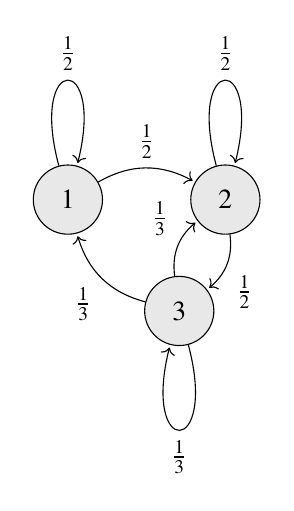
\begin{tikzpicture}[shorten >=1pt,node distance=2cm, scale =3, auto]
			\tikzstyle{every state}=[fill={rgb:black,1;white,10}]
			
			\node[state]   (q_1)                          {$1$};
			\node[state]   (q_2)  [right of=q_1]          {$2$};
			\node[state]   (q_3)  [below right of=q_1]          {$3$};
			
			\path[->]
			(q_1) edge [loop above] node {$\frac{1}{2}$}    (   )
			edge [bend left]  node {$\frac{1}{2}$}    (q_2)
			(q_2) edge [bend left]  node {$\frac{1}{2}$}    (q_3)
			edge [loop above] node {$\frac{1}{2}$}    ()
			(q_3) edge [bend left]  node {$\frac{1}{3}$}    (q_2)
			edge [bend left]  node {$\frac{1}{3}$}    (q_1)
			edge [loop below] node {$\frac{1}{3}$}    ();
		\end{tikzpicture}$
		
		\\  
		&\\
		&\\
		\hline
		\multirow{3}{*}{Checking whether the  } & \\
		& Here,\\chain is Irreducible
		& All the states are accessible to one another. \\and Aperiodic
		& $\implies$ They are in the same communication class. So, it is Irreducible.\\
		& \\
		& There exists the non- zero self-transition, which means that the chain \\
		& is Aperiodic.\\
		&\\ 
		& We know that if the Markov Chain is irreducible and aperiodic then \\
		& \qquad \qquad \qquad $\Vec{\pi}_{j} = \lim_{n \to \infty}P\{X_{n} = j\}$, $j = 1,...,N$ \\
		& These are the stationary probabilities. \\
		&\\
		\hline
		\multirow{3}{*}{Finding the Stationary} & \\
		& Stationary Probability can be represented as\\Probability Distributions
		& \qquad \qquad \qquad $\Vec{\pi} = \Vec{\pi} \vec{P}$\\
		& \\
		& \qquad $\implies$ $\myvec{v_{1}&&v_{2}&&v_{3}} = \myvec{v_{1}&&v_{2}&&v_{3}}\vec{P}$ \\
		& \\
		& Equating the above equation we get \\
		& \\
		& \qquad \qquad \qquad $\frac{1}{2}v_{1}-\frac{1}{3}v_{3} = 0$ $\label{eq:solutions/2018/dec/106/eq}$\\
		& \\
		& \qquad \qquad \qquad $\frac{1}{2}v_{1}-\frac{1}{2}v_{2} + \frac{1}{3}v_{3} = 0$\\
		& \\
		& \qquad \qquad \qquad $\frac{1}{2}v_{2}-\frac{2}{3}v_{3} = 0$\\
		& \\\
		& We see that summation of second and the third equation gives us the \\
		& first equation only. \\
		& And we know that the probability distribution will sum up to 1. \\
		& \\
		& \qquad \qquad \qquad $v_{1}+v_{2}+v_{3} = 1$ \\
		& \\
		& Therefore, we get the equation form as \\
		& \\
		& \qquad \qquad \qquad $\myvec{1&1&1\\\frac{1}{2}&0&\frac{-1}{3}\\\frac{1}{2}&\frac{-1}{2}&\frac{1}{3}}\myvec{v_{1}\\v_{2}\\v_{3}} = \myvec{1\\0\\0}$ \\
		& \\
		\hline
		\multirow{3}{*}{Solving the linear} & \\
		& The above linear equation can be solved using Gauss-Jordan method as\\equtions
		& \\
		& \qquad \qquad \qquad $\myvec{1&1&1&\vrule&1\\\frac{1}{2}&0&\frac{-1}{3}&\vrule&0\\\frac{1}{2}&\frac{-1}{2}&\frac{1}{3}&\vrule&0}$\\
		& \\
		& \qquad $\xleftrightarrow[]{R_2 \leftarrow R_2 - \frac{1}{2}R_1}$
		$\myvec{1&1&1&\vrule&1\\0&\frac{-1}{2}&\frac{-5}{6}&\vrule&\frac{-1}{2}\\\frac{1}{2}&\frac{-1}{2}&\frac{1}{3}&\vrule&0}$\\
		&\\
		& \qquad $\xleftrightarrow[]{R_3 \leftarrow R_3 - \frac{1}{2}R_1}$
		$\myvec{1&1&1&\vrule&1\\0&\frac{-1}{2}&\frac{-5}{6}&\vrule&\frac{-1}{2}\\0&-1&\frac{-1}{6}&\vrule&\frac{-1}{2}}$\\
		&\\
		& \qquad $\xleftrightarrow[]{R_2 \leftarrow \frac{-1}{2}R_2}$
		$\myvec{1&1&1&\vrule&1\\0&1&\frac{5}{3}&\vrule&1\\0&-1&\frac{-1}{6}&\vrule&\frac{-1}{2}}$\\
		&\\
		& \qquad $\xleftrightarrow[]{R_3 \leftarrow R_3 + R_2}$
		$\myvec{1&1&1&\vrule&1\\0&1&\frac{5}{3}&\vrule&1\\0&0&\frac{3}{2}&\vrule&\frac{1}{2}}$\\
		&\\
		& \qquad $\xleftrightarrow[]{R_3 \leftarrow \frac{3}{2}R_3}$
		$\myvec{1&1&1&\vrule&1\\0&1&\frac{5}{3}&\vrule&1\\0&0&1&\vrule&\frac{1}{3}}$\\
		&\\
		& \qquad $\xleftrightarrow[]{R_2 \leftarrow R_2 - \frac{5}{3}R_3}$
		$\myvec{1&1&1&\vrule&1\\0&1&0&\vrule&\frac{4}{9}\\0&0&1&\vrule&\frac{1}{3}}$\\
		&\\
		& \qquad $\xleftrightarrow[]{R_1 \leftarrow R_1 - R_3}$
		$\myvec{1&1&0&\vrule&\frac{2}{3}\\0&1&0&\vrule&\frac{4}{9}\\0&0&1&\vrule&\frac{1}{3}}$\\
		&\\
		& \qquad $\xleftrightarrow[]{R_1 \leftarrow R_1 - R_2}$
		$\myvec{1&0&0&\vrule&\frac{2}{9}\\0&1&0&\vrule&\frac{4}{9}\\0&0&1&\vrule&\frac{1}{3}}$\\
		&\\
		& $\therefore$, stationary probability distribution $\pi$ is given by \\
		& \qquad \qquad $\pi = \myvec{\frac{2}{9} & \frac{4}{9} & \frac{1}{3}}$ \\
		& \\
		\hline
		\multirow{3}{*}{Observations} & \\
		
		
		& Since the given transition probability matrix $\vec{P}$ is irreducible and aperiodic, \\
		& then $\lim_{n \to \infty} \vec{P}^{n}$ converges to a matrix with all rows identical and equal to $\vec{\pi}$. \\
		& \\
		& We were able to find $\vec{\pi}$ as $\myvec{\frac{2}{9} & \frac{4}{9} & \frac{1}{3}}$ \\
		& \\
		& $\lim_{n \to \infty} \vec{P}^{n} = \myvec{\frac{2}{9}&\frac{4}{9}&\frac{1}{3}\\\frac{2}{9}&\frac{4}{9}&\frac{1}{3}\\\frac{2}{9}&\frac{4}{9}&\frac{1}{3}}$\\
		& \\
		& From the above matrix, we get \\
		& \\
		& $\lim_{n \to \infty} \vec{P}^{n}_{11} = \frac{2}{9}$ \\
		&\\
		& $\lim_{n \to \infty} \vec{P}^{n}_{21} = \frac{2}{9}$ \\
		&\\
		& $\lim_{n \to \infty} \vec{P}^{n}_{32} = \frac{4}{9}$ \\
		&\\
		& $\lim_{n \to \infty} \vec{P}^{n}_{13} = \frac{1}{3}$ \\
		&\\
		\hline
		\multirow{3}{*}{Conclusion} & \\
		& From our observation we see that \\
		&\\
		& Options 1) and 4) are True.\\
		& \\
		\hline
\caption{}
\label{eq:solutions/2018/dec/106/table1}
	\end{longtable}
\twocolumn

\item For any $n\times n$ matrix $B$, let $N(B)=\{X\in \mathbb{R}^n:BX=0\}$ be the null space of $B$. Let $A$ be a $4\times 4$ matrix with $dim(N(A-4I))=2, dim(N(A-2I))=1$ and $rank(A)=3$
Which of the following are true?
\begin{enumerate}
\item 0,2 and 4 are eigenvalues of A
\item determinant(A)=0
\item A is not diagonalizable
\item trace(A)=8
\end{enumerate}
%
\solution
See Tables \ref{eq:solutions/2018/dec/106/table0} and \ref{eq:solutions/2018/dec/106/table1}


\onecolumn
	\begin{longtable}{|l|l|}
		\hline
		\multirow{3}{*}{Irreducible Markov Chain} 
		& \\
		& A Markov chain is $\textbf{irreducible}$ if all the states communicate with each other,\\
		& i.e., if there is only one communication class.\\
		&\\
		\hline
		\multirow{3}{*}{Aperiodic Markov Chain} & \\
		& If there is a self-transition in the chain ($p^{ii}>0$ for some i), then the chain is\\
		& called as $\textbf{aperiodic}$\\
		& \\
		\hline
		\multirow{3}{*}{Stationary Distribution} & \\
		& A stationary distribution of a Markov chain is a probability distribution that\\
		& remains unchanged in the Markov chain as time progresses. Typically, it is\\
		& represented as a row vector $\Vec{\pi}$ whose entries are probabilities summing to 1,\\ 
		& and given transition matrix $\textbf{P}$, it satisfies\\
		& \\
		&  \qquad \qquad  \qquad$\Vec{\pi} = \Vec{\pi} \textbf{P}$\\
		& \\
		\hline
\caption{}
\label{eq:solutions/2018/dec/106/table0}
	\end{longtable}
	\begin{longtable}{|l|l|}
		\hline
		\multirow{3}{*}{Drawing Transition diagram} 
		& \\
		& 
		
		$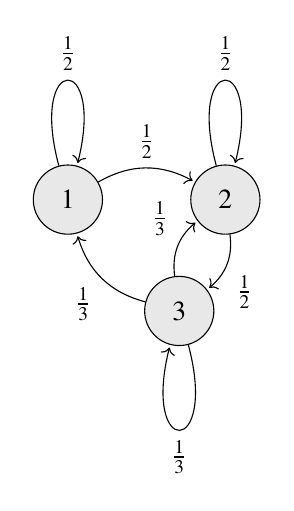
\begin{tikzpicture}[shorten >=1pt,node distance=2cm, scale =3, auto]
			\tikzstyle{every state}=[fill={rgb:black,1;white,10}]
			
			\node[state]   (q_1)                          {$1$};
			\node[state]   (q_2)  [right of=q_1]          {$2$};
			\node[state]   (q_3)  [below right of=q_1]          {$3$};
			
			\path[->]
			(q_1) edge [loop above] node {$\frac{1}{2}$}    (   )
			edge [bend left]  node {$\frac{1}{2}$}    (q_2)
			(q_2) edge [bend left]  node {$\frac{1}{2}$}    (q_3)
			edge [loop above] node {$\frac{1}{2}$}    ()
			(q_3) edge [bend left]  node {$\frac{1}{3}$}    (q_2)
			edge [bend left]  node {$\frac{1}{3}$}    (q_1)
			edge [loop below] node {$\frac{1}{3}$}    ();
		\end{tikzpicture}$
		
		\\  
		&\\
		&\\
		\hline
		\multirow{3}{*}{Checking whether the  } & \\
		& Here,\\chain is Irreducible
		& All the states are accessible to one another. \\and Aperiodic
		& $\implies$ They are in the same communication class. So, it is Irreducible.\\
		& \\
		& There exists the non- zero self-transition, which means that the chain \\
		& is Aperiodic.\\
		&\\ 
		& We know that if the Markov Chain is irreducible and aperiodic then \\
		& \qquad \qquad \qquad $\Vec{\pi}_{j} = \lim_{n \to \infty}P\{X_{n} = j\}$, $j = 1,...,N$ \\
		& These are the stationary probabilities. \\
		&\\
		\hline
		\multirow{3}{*}{Finding the Stationary} & \\
		& Stationary Probability can be represented as\\Probability Distributions
		& \qquad \qquad \qquad $\Vec{\pi} = \Vec{\pi} \vec{P}$\\
		& \\
		& \qquad $\implies$ $\myvec{v_{1}&&v_{2}&&v_{3}} = \myvec{v_{1}&&v_{2}&&v_{3}}\vec{P}$ \\
		& \\
		& Equating the above equation we get \\
		& \\
		& \qquad \qquad \qquad $\frac{1}{2}v_{1}-\frac{1}{3}v_{3} = 0$ $\label{eq:solutions/2018/dec/106/eq}$\\
		& \\
		& \qquad \qquad \qquad $\frac{1}{2}v_{1}-\frac{1}{2}v_{2} + \frac{1}{3}v_{3} = 0$\\
		& \\
		& \qquad \qquad \qquad $\frac{1}{2}v_{2}-\frac{2}{3}v_{3} = 0$\\
		& \\\
		& We see that summation of second and the third equation gives us the \\
		& first equation only. \\
		& And we know that the probability distribution will sum up to 1. \\
		& \\
		& \qquad \qquad \qquad $v_{1}+v_{2}+v_{3} = 1$ \\
		& \\
		& Therefore, we get the equation form as \\
		& \\
		& \qquad \qquad \qquad $\myvec{1&1&1\\\frac{1}{2}&0&\frac{-1}{3}\\\frac{1}{2}&\frac{-1}{2}&\frac{1}{3}}\myvec{v_{1}\\v_{2}\\v_{3}} = \myvec{1\\0\\0}$ \\
		& \\
		\hline
		\multirow{3}{*}{Solving the linear} & \\
		& The above linear equation can be solved using Gauss-Jordan method as\\equtions
		& \\
		& \qquad \qquad \qquad $\myvec{1&1&1&\vrule&1\\\frac{1}{2}&0&\frac{-1}{3}&\vrule&0\\\frac{1}{2}&\frac{-1}{2}&\frac{1}{3}&\vrule&0}$\\
		& \\
		& \qquad $\xleftrightarrow[]{R_2 \leftarrow R_2 - \frac{1}{2}R_1}$
		$\myvec{1&1&1&\vrule&1\\0&\frac{-1}{2}&\frac{-5}{6}&\vrule&\frac{-1}{2}\\\frac{1}{2}&\frac{-1}{2}&\frac{1}{3}&\vrule&0}$\\
		&\\
		& \qquad $\xleftrightarrow[]{R_3 \leftarrow R_3 - \frac{1}{2}R_1}$
		$\myvec{1&1&1&\vrule&1\\0&\frac{-1}{2}&\frac{-5}{6}&\vrule&\frac{-1}{2}\\0&-1&\frac{-1}{6}&\vrule&\frac{-1}{2}}$\\
		&\\
		& \qquad $\xleftrightarrow[]{R_2 \leftarrow \frac{-1}{2}R_2}$
		$\myvec{1&1&1&\vrule&1\\0&1&\frac{5}{3}&\vrule&1\\0&-1&\frac{-1}{6}&\vrule&\frac{-1}{2}}$\\
		&\\
		& \qquad $\xleftrightarrow[]{R_3 \leftarrow R_3 + R_2}$
		$\myvec{1&1&1&\vrule&1\\0&1&\frac{5}{3}&\vrule&1\\0&0&\frac{3}{2}&\vrule&\frac{1}{2}}$\\
		&\\
		& \qquad $\xleftrightarrow[]{R_3 \leftarrow \frac{3}{2}R_3}$
		$\myvec{1&1&1&\vrule&1\\0&1&\frac{5}{3}&\vrule&1\\0&0&1&\vrule&\frac{1}{3}}$\\
		&\\
		& \qquad $\xleftrightarrow[]{R_2 \leftarrow R_2 - \frac{5}{3}R_3}$
		$\myvec{1&1&1&\vrule&1\\0&1&0&\vrule&\frac{4}{9}\\0&0&1&\vrule&\frac{1}{3}}$\\
		&\\
		& \qquad $\xleftrightarrow[]{R_1 \leftarrow R_1 - R_3}$
		$\myvec{1&1&0&\vrule&\frac{2}{3}\\0&1&0&\vrule&\frac{4}{9}\\0&0&1&\vrule&\frac{1}{3}}$\\
		&\\
		& \qquad $\xleftrightarrow[]{R_1 \leftarrow R_1 - R_2}$
		$\myvec{1&0&0&\vrule&\frac{2}{9}\\0&1&0&\vrule&\frac{4}{9}\\0&0&1&\vrule&\frac{1}{3}}$\\
		&\\
		& $\therefore$, stationary probability distribution $\pi$ is given by \\
		& \qquad \qquad $\pi = \myvec{\frac{2}{9} & \frac{4}{9} & \frac{1}{3}}$ \\
		& \\
		\hline
		\multirow{3}{*}{Observations} & \\
		
		
		& Since the given transition probability matrix $\vec{P}$ is irreducible and aperiodic, \\
		& then $\lim_{n \to \infty} \vec{P}^{n}$ converges to a matrix with all rows identical and equal to $\vec{\pi}$. \\
		& \\
		& We were able to find $\vec{\pi}$ as $\myvec{\frac{2}{9} & \frac{4}{9} & \frac{1}{3}}$ \\
		& \\
		& $\lim_{n \to \infty} \vec{P}^{n} = \myvec{\frac{2}{9}&\frac{4}{9}&\frac{1}{3}\\\frac{2}{9}&\frac{4}{9}&\frac{1}{3}\\\frac{2}{9}&\frac{4}{9}&\frac{1}{3}}$\\
		& \\
		& From the above matrix, we get \\
		& \\
		& $\lim_{n \to \infty} \vec{P}^{n}_{11} = \frac{2}{9}$ \\
		&\\
		& $\lim_{n \to \infty} \vec{P}^{n}_{21} = \frac{2}{9}$ \\
		&\\
		& $\lim_{n \to \infty} \vec{P}^{n}_{32} = \frac{4}{9}$ \\
		&\\
		& $\lim_{n \to \infty} \vec{P}^{n}_{13} = \frac{1}{3}$ \\
		&\\
		\hline
		\multirow{3}{*}{Conclusion} & \\
		& From our observation we see that \\
		&\\
		& Options 1) and 4) are True.\\
		& \\
		\hline
\caption{}
\label{eq:solutions/2018/dec/106/table1}
	\end{longtable}
\twocolumn

\item Which of the following 3x3 matrices are diagonizable over $\mathbb{R}?$\\
\begin{enumerate}
    \item \myvec{1&2&3\\0&4&5\\0&0&6}
    \item \myvec{0&1&0\\-1&0&0\\0&0&1}
    \item \myvec{1&2&3\\2&1&4\\3&4&1}
    \item \myvec{0&1&2\\0&0&1\\0&0&0}
\end{enumerate}
%
\solution
See Tables \ref{eq:solutions/2018/dec/106/table0} and \ref{eq:solutions/2018/dec/106/table1}


\onecolumn
	\begin{longtable}{|l|l|}
		\hline
		\multirow{3}{*}{Irreducible Markov Chain} 
		& \\
		& A Markov chain is $\textbf{irreducible}$ if all the states communicate with each other,\\
		& i.e., if there is only one communication class.\\
		&\\
		\hline
		\multirow{3}{*}{Aperiodic Markov Chain} & \\
		& If there is a self-transition in the chain ($p^{ii}>0$ for some i), then the chain is\\
		& called as $\textbf{aperiodic}$\\
		& \\
		\hline
		\multirow{3}{*}{Stationary Distribution} & \\
		& A stationary distribution of a Markov chain is a probability distribution that\\
		& remains unchanged in the Markov chain as time progresses. Typically, it is\\
		& represented as a row vector $\Vec{\pi}$ whose entries are probabilities summing to 1,\\ 
		& and given transition matrix $\textbf{P}$, it satisfies\\
		& \\
		&  \qquad \qquad  \qquad$\Vec{\pi} = \Vec{\pi} \textbf{P}$\\
		& \\
		\hline
\caption{}
\label{eq:solutions/2018/dec/106/table0}
	\end{longtable}
	\begin{longtable}{|l|l|}
		\hline
		\multirow{3}{*}{Drawing Transition diagram} 
		& \\
		& 
		
		$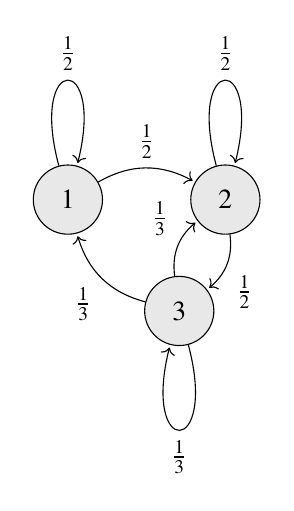
\begin{tikzpicture}[shorten >=1pt,node distance=2cm, scale =3, auto]
			\tikzstyle{every state}=[fill={rgb:black,1;white,10}]
			
			\node[state]   (q_1)                          {$1$};
			\node[state]   (q_2)  [right of=q_1]          {$2$};
			\node[state]   (q_3)  [below right of=q_1]          {$3$};
			
			\path[->]
			(q_1) edge [loop above] node {$\frac{1}{2}$}    (   )
			edge [bend left]  node {$\frac{1}{2}$}    (q_2)
			(q_2) edge [bend left]  node {$\frac{1}{2}$}    (q_3)
			edge [loop above] node {$\frac{1}{2}$}    ()
			(q_3) edge [bend left]  node {$\frac{1}{3}$}    (q_2)
			edge [bend left]  node {$\frac{1}{3}$}    (q_1)
			edge [loop below] node {$\frac{1}{3}$}    ();
		\end{tikzpicture}$
		
		\\  
		&\\
		&\\
		\hline
		\multirow{3}{*}{Checking whether the  } & \\
		& Here,\\chain is Irreducible
		& All the states are accessible to one another. \\and Aperiodic
		& $\implies$ They are in the same communication class. So, it is Irreducible.\\
		& \\
		& There exists the non- zero self-transition, which means that the chain \\
		& is Aperiodic.\\
		&\\ 
		& We know that if the Markov Chain is irreducible and aperiodic then \\
		& \qquad \qquad \qquad $\Vec{\pi}_{j} = \lim_{n \to \infty}P\{X_{n} = j\}$, $j = 1,...,N$ \\
		& These are the stationary probabilities. \\
		&\\
		\hline
		\multirow{3}{*}{Finding the Stationary} & \\
		& Stationary Probability can be represented as\\Probability Distributions
		& \qquad \qquad \qquad $\Vec{\pi} = \Vec{\pi} \vec{P}$\\
		& \\
		& \qquad $\implies$ $\myvec{v_{1}&&v_{2}&&v_{3}} = \myvec{v_{1}&&v_{2}&&v_{3}}\vec{P}$ \\
		& \\
		& Equating the above equation we get \\
		& \\
		& \qquad \qquad \qquad $\frac{1}{2}v_{1}-\frac{1}{3}v_{3} = 0$ $\label{eq:solutions/2018/dec/106/eq}$\\
		& \\
		& \qquad \qquad \qquad $\frac{1}{2}v_{1}-\frac{1}{2}v_{2} + \frac{1}{3}v_{3} = 0$\\
		& \\
		& \qquad \qquad \qquad $\frac{1}{2}v_{2}-\frac{2}{3}v_{3} = 0$\\
		& \\\
		& We see that summation of second and the third equation gives us the \\
		& first equation only. \\
		& And we know that the probability distribution will sum up to 1. \\
		& \\
		& \qquad \qquad \qquad $v_{1}+v_{2}+v_{3} = 1$ \\
		& \\
		& Therefore, we get the equation form as \\
		& \\
		& \qquad \qquad \qquad $\myvec{1&1&1\\\frac{1}{2}&0&\frac{-1}{3}\\\frac{1}{2}&\frac{-1}{2}&\frac{1}{3}}\myvec{v_{1}\\v_{2}\\v_{3}} = \myvec{1\\0\\0}$ \\
		& \\
		\hline
		\multirow{3}{*}{Solving the linear} & \\
		& The above linear equation can be solved using Gauss-Jordan method as\\equtions
		& \\
		& \qquad \qquad \qquad $\myvec{1&1&1&\vrule&1\\\frac{1}{2}&0&\frac{-1}{3}&\vrule&0\\\frac{1}{2}&\frac{-1}{2}&\frac{1}{3}&\vrule&0}$\\
		& \\
		& \qquad $\xleftrightarrow[]{R_2 \leftarrow R_2 - \frac{1}{2}R_1}$
		$\myvec{1&1&1&\vrule&1\\0&\frac{-1}{2}&\frac{-5}{6}&\vrule&\frac{-1}{2}\\\frac{1}{2}&\frac{-1}{2}&\frac{1}{3}&\vrule&0}$\\
		&\\
		& \qquad $\xleftrightarrow[]{R_3 \leftarrow R_3 - \frac{1}{2}R_1}$
		$\myvec{1&1&1&\vrule&1\\0&\frac{-1}{2}&\frac{-5}{6}&\vrule&\frac{-1}{2}\\0&-1&\frac{-1}{6}&\vrule&\frac{-1}{2}}$\\
		&\\
		& \qquad $\xleftrightarrow[]{R_2 \leftarrow \frac{-1}{2}R_2}$
		$\myvec{1&1&1&\vrule&1\\0&1&\frac{5}{3}&\vrule&1\\0&-1&\frac{-1}{6}&\vrule&\frac{-1}{2}}$\\
		&\\
		& \qquad $\xleftrightarrow[]{R_3 \leftarrow R_3 + R_2}$
		$\myvec{1&1&1&\vrule&1\\0&1&\frac{5}{3}&\vrule&1\\0&0&\frac{3}{2}&\vrule&\frac{1}{2}}$\\
		&\\
		& \qquad $\xleftrightarrow[]{R_3 \leftarrow \frac{3}{2}R_3}$
		$\myvec{1&1&1&\vrule&1\\0&1&\frac{5}{3}&\vrule&1\\0&0&1&\vrule&\frac{1}{3}}$\\
		&\\
		& \qquad $\xleftrightarrow[]{R_2 \leftarrow R_2 - \frac{5}{3}R_3}$
		$\myvec{1&1&1&\vrule&1\\0&1&0&\vrule&\frac{4}{9}\\0&0&1&\vrule&\frac{1}{3}}$\\
		&\\
		& \qquad $\xleftrightarrow[]{R_1 \leftarrow R_1 - R_3}$
		$\myvec{1&1&0&\vrule&\frac{2}{3}\\0&1&0&\vrule&\frac{4}{9}\\0&0&1&\vrule&\frac{1}{3}}$\\
		&\\
		& \qquad $\xleftrightarrow[]{R_1 \leftarrow R_1 - R_2}$
		$\myvec{1&0&0&\vrule&\frac{2}{9}\\0&1&0&\vrule&\frac{4}{9}\\0&0&1&\vrule&\frac{1}{3}}$\\
		&\\
		& $\therefore$, stationary probability distribution $\pi$ is given by \\
		& \qquad \qquad $\pi = \myvec{\frac{2}{9} & \frac{4}{9} & \frac{1}{3}}$ \\
		& \\
		\hline
		\multirow{3}{*}{Observations} & \\
		
		
		& Since the given transition probability matrix $\vec{P}$ is irreducible and aperiodic, \\
		& then $\lim_{n \to \infty} \vec{P}^{n}$ converges to a matrix with all rows identical and equal to $\vec{\pi}$. \\
		& \\
		& We were able to find $\vec{\pi}$ as $\myvec{\frac{2}{9} & \frac{4}{9} & \frac{1}{3}}$ \\
		& \\
		& $\lim_{n \to \infty} \vec{P}^{n} = \myvec{\frac{2}{9}&\frac{4}{9}&\frac{1}{3}\\\frac{2}{9}&\frac{4}{9}&\frac{1}{3}\\\frac{2}{9}&\frac{4}{9}&\frac{1}{3}}$\\
		& \\
		& From the above matrix, we get \\
		& \\
		& $\lim_{n \to \infty} \vec{P}^{n}_{11} = \frac{2}{9}$ \\
		&\\
		& $\lim_{n \to \infty} \vec{P}^{n}_{21} = \frac{2}{9}$ \\
		&\\
		& $\lim_{n \to \infty} \vec{P}^{n}_{32} = \frac{4}{9}$ \\
		&\\
		& $\lim_{n \to \infty} \vec{P}^{n}_{13} = \frac{1}{3}$ \\
		&\\
		\hline
		\multirow{3}{*}{Conclusion} & \\
		& From our observation we see that \\
		&\\
		& Options 1) and 4) are True.\\
		& \\
		\hline
\caption{}
\label{eq:solutions/2018/dec/106/table1}
	\end{longtable}
\twocolumn

\twocolumn
\item Let $\vec{A} = \myvec{3 & 1 & 2 \\ 1 & 2 & 3 \\ 2 & 3 & 1  }$ and $\vec{Q(X) = X^TAX}$ for $\vec{X} \in \mathbb{R}^{3}$. Then
\begin{enumerate}
	\item $\vec{A}$ has exactly two positive eigen values.
	\item all the eigen values of $\vec{A}$ are positive.
	\item $\vec{Q(X)} \geq 0 $ $\forall$ $\vec{X}$ $\in$ $\mathbb{R}^3$
	\item $\vec{Q(X)} < 0 $ for some $\vec{X}$ $\in$ $\mathbb{R}^3$
\end{enumerate}
%
%
\solution
See Tables \ref{eq:solutions/2018/dec/106/table0} and \ref{eq:solutions/2018/dec/106/table1}


\onecolumn
	\begin{longtable}{|l|l|}
		\hline
		\multirow{3}{*}{Irreducible Markov Chain} 
		& \\
		& A Markov chain is $\textbf{irreducible}$ if all the states communicate with each other,\\
		& i.e., if there is only one communication class.\\
		&\\
		\hline
		\multirow{3}{*}{Aperiodic Markov Chain} & \\
		& If there is a self-transition in the chain ($p^{ii}>0$ for some i), then the chain is\\
		& called as $\textbf{aperiodic}$\\
		& \\
		\hline
		\multirow{3}{*}{Stationary Distribution} & \\
		& A stationary distribution of a Markov chain is a probability distribution that\\
		& remains unchanged in the Markov chain as time progresses. Typically, it is\\
		& represented as a row vector $\Vec{\pi}$ whose entries are probabilities summing to 1,\\ 
		& and given transition matrix $\textbf{P}$, it satisfies\\
		& \\
		&  \qquad \qquad  \qquad$\Vec{\pi} = \Vec{\pi} \textbf{P}$\\
		& \\
		\hline
\caption{}
\label{eq:solutions/2018/dec/106/table0}
	\end{longtable}
	\begin{longtable}{|l|l|}
		\hline
		\multirow{3}{*}{Drawing Transition diagram} 
		& \\
		& 
		
		$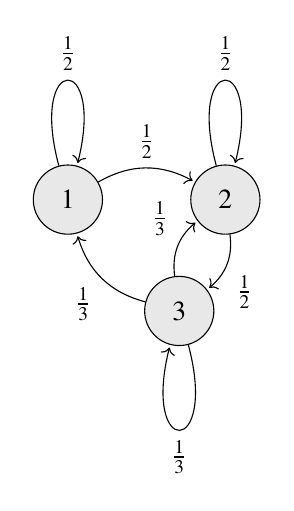
\begin{tikzpicture}[shorten >=1pt,node distance=2cm, scale =3, auto]
			\tikzstyle{every state}=[fill={rgb:black,1;white,10}]
			
			\node[state]   (q_1)                          {$1$};
			\node[state]   (q_2)  [right of=q_1]          {$2$};
			\node[state]   (q_3)  [below right of=q_1]          {$3$};
			
			\path[->]
			(q_1) edge [loop above] node {$\frac{1}{2}$}    (   )
			edge [bend left]  node {$\frac{1}{2}$}    (q_2)
			(q_2) edge [bend left]  node {$\frac{1}{2}$}    (q_3)
			edge [loop above] node {$\frac{1}{2}$}    ()
			(q_3) edge [bend left]  node {$\frac{1}{3}$}    (q_2)
			edge [bend left]  node {$\frac{1}{3}$}    (q_1)
			edge [loop below] node {$\frac{1}{3}$}    ();
		\end{tikzpicture}$
		
		\\  
		&\\
		&\\
		\hline
		\multirow{3}{*}{Checking whether the  } & \\
		& Here,\\chain is Irreducible
		& All the states are accessible to one another. \\and Aperiodic
		& $\implies$ They are in the same communication class. So, it is Irreducible.\\
		& \\
		& There exists the non- zero self-transition, which means that the chain \\
		& is Aperiodic.\\
		&\\ 
		& We know that if the Markov Chain is irreducible and aperiodic then \\
		& \qquad \qquad \qquad $\Vec{\pi}_{j} = \lim_{n \to \infty}P\{X_{n} = j\}$, $j = 1,...,N$ \\
		& These are the stationary probabilities. \\
		&\\
		\hline
		\multirow{3}{*}{Finding the Stationary} & \\
		& Stationary Probability can be represented as\\Probability Distributions
		& \qquad \qquad \qquad $\Vec{\pi} = \Vec{\pi} \vec{P}$\\
		& \\
		& \qquad $\implies$ $\myvec{v_{1}&&v_{2}&&v_{3}} = \myvec{v_{1}&&v_{2}&&v_{3}}\vec{P}$ \\
		& \\
		& Equating the above equation we get \\
		& \\
		& \qquad \qquad \qquad $\frac{1}{2}v_{1}-\frac{1}{3}v_{3} = 0$ $\label{eq:solutions/2018/dec/106/eq}$\\
		& \\
		& \qquad \qquad \qquad $\frac{1}{2}v_{1}-\frac{1}{2}v_{2} + \frac{1}{3}v_{3} = 0$\\
		& \\
		& \qquad \qquad \qquad $\frac{1}{2}v_{2}-\frac{2}{3}v_{3} = 0$\\
		& \\\
		& We see that summation of second and the third equation gives us the \\
		& first equation only. \\
		& And we know that the probability distribution will sum up to 1. \\
		& \\
		& \qquad \qquad \qquad $v_{1}+v_{2}+v_{3} = 1$ \\
		& \\
		& Therefore, we get the equation form as \\
		& \\
		& \qquad \qquad \qquad $\myvec{1&1&1\\\frac{1}{2}&0&\frac{-1}{3}\\\frac{1}{2}&\frac{-1}{2}&\frac{1}{3}}\myvec{v_{1}\\v_{2}\\v_{3}} = \myvec{1\\0\\0}$ \\
		& \\
		\hline
		\multirow{3}{*}{Solving the linear} & \\
		& The above linear equation can be solved using Gauss-Jordan method as\\equtions
		& \\
		& \qquad \qquad \qquad $\myvec{1&1&1&\vrule&1\\\frac{1}{2}&0&\frac{-1}{3}&\vrule&0\\\frac{1}{2}&\frac{-1}{2}&\frac{1}{3}&\vrule&0}$\\
		& \\
		& \qquad $\xleftrightarrow[]{R_2 \leftarrow R_2 - \frac{1}{2}R_1}$
		$\myvec{1&1&1&\vrule&1\\0&\frac{-1}{2}&\frac{-5}{6}&\vrule&\frac{-1}{2}\\\frac{1}{2}&\frac{-1}{2}&\frac{1}{3}&\vrule&0}$\\
		&\\
		& \qquad $\xleftrightarrow[]{R_3 \leftarrow R_3 - \frac{1}{2}R_1}$
		$\myvec{1&1&1&\vrule&1\\0&\frac{-1}{2}&\frac{-5}{6}&\vrule&\frac{-1}{2}\\0&-1&\frac{-1}{6}&\vrule&\frac{-1}{2}}$\\
		&\\
		& \qquad $\xleftrightarrow[]{R_2 \leftarrow \frac{-1}{2}R_2}$
		$\myvec{1&1&1&\vrule&1\\0&1&\frac{5}{3}&\vrule&1\\0&-1&\frac{-1}{6}&\vrule&\frac{-1}{2}}$\\
		&\\
		& \qquad $\xleftrightarrow[]{R_3 \leftarrow R_3 + R_2}$
		$\myvec{1&1&1&\vrule&1\\0&1&\frac{5}{3}&\vrule&1\\0&0&\frac{3}{2}&\vrule&\frac{1}{2}}$\\
		&\\
		& \qquad $\xleftrightarrow[]{R_3 \leftarrow \frac{3}{2}R_3}$
		$\myvec{1&1&1&\vrule&1\\0&1&\frac{5}{3}&\vrule&1\\0&0&1&\vrule&\frac{1}{3}}$\\
		&\\
		& \qquad $\xleftrightarrow[]{R_2 \leftarrow R_2 - \frac{5}{3}R_3}$
		$\myvec{1&1&1&\vrule&1\\0&1&0&\vrule&\frac{4}{9}\\0&0&1&\vrule&\frac{1}{3}}$\\
		&\\
		& \qquad $\xleftrightarrow[]{R_1 \leftarrow R_1 - R_3}$
		$\myvec{1&1&0&\vrule&\frac{2}{3}\\0&1&0&\vrule&\frac{4}{9}\\0&0&1&\vrule&\frac{1}{3}}$\\
		&\\
		& \qquad $\xleftrightarrow[]{R_1 \leftarrow R_1 - R_2}$
		$\myvec{1&0&0&\vrule&\frac{2}{9}\\0&1&0&\vrule&\frac{4}{9}\\0&0&1&\vrule&\frac{1}{3}}$\\
		&\\
		& $\therefore$, stationary probability distribution $\pi$ is given by \\
		& \qquad \qquad $\pi = \myvec{\frac{2}{9} & \frac{4}{9} & \frac{1}{3}}$ \\
		& \\
		\hline
		\multirow{3}{*}{Observations} & \\
		
		
		& Since the given transition probability matrix $\vec{P}$ is irreducible and aperiodic, \\
		& then $\lim_{n \to \infty} \vec{P}^{n}$ converges to a matrix with all rows identical and equal to $\vec{\pi}$. \\
		& \\
		& We were able to find $\vec{\pi}$ as $\myvec{\frac{2}{9} & \frac{4}{9} & \frac{1}{3}}$ \\
		& \\
		& $\lim_{n \to \infty} \vec{P}^{n} = \myvec{\frac{2}{9}&\frac{4}{9}&\frac{1}{3}\\\frac{2}{9}&\frac{4}{9}&\frac{1}{3}\\\frac{2}{9}&\frac{4}{9}&\frac{1}{3}}$\\
		& \\
		& From the above matrix, we get \\
		& \\
		& $\lim_{n \to \infty} \vec{P}^{n}_{11} = \frac{2}{9}$ \\
		&\\
		& $\lim_{n \to \infty} \vec{P}^{n}_{21} = \frac{2}{9}$ \\
		&\\
		& $\lim_{n \to \infty} \vec{P}^{n}_{32} = \frac{4}{9}$ \\
		&\\
		& $\lim_{n \to \infty} \vec{P}^{n}_{13} = \frac{1}{3}$ \\
		&\\
		\hline
		\multirow{3}{*}{Conclusion} & \\
		& From our observation we see that \\
		&\\
		& Options 1) and 4) are True.\\
		& \\
		\hline
\caption{}
\label{eq:solutions/2018/dec/106/table1}
	\end{longtable}
\twocolumn

\item Consider the matrix
\begin{align}
A(x) = \myvec{1+x^2&7&11\\3x&2x&4\\8x&17&13} & ;x\in \vec{R}.
\end{align}
Then,
\begin{enumerate}
\item A(x) has eigenvalue 0 for some $x\in \vec{R}$.
\item 0 is not an eigenvalue of A(x) for any $x\in \vec{R}$.
\item A(x) has eigenvalue 0 $\forall x\in \vec{R}$.
\item A(x) is invertible $\forall x\in \vec{R}$.
\end{enumerate}
%
\solution
See Tables \ref{eq:solutions/2018/dec/106/table0} and \ref{eq:solutions/2018/dec/106/table1}


\onecolumn
	\begin{longtable}{|l|l|}
		\hline
		\multirow{3}{*}{Irreducible Markov Chain} 
		& \\
		& A Markov chain is $\textbf{irreducible}$ if all the states communicate with each other,\\
		& i.e., if there is only one communication class.\\
		&\\
		\hline
		\multirow{3}{*}{Aperiodic Markov Chain} & \\
		& If there is a self-transition in the chain ($p^{ii}>0$ for some i), then the chain is\\
		& called as $\textbf{aperiodic}$\\
		& \\
		\hline
		\multirow{3}{*}{Stationary Distribution} & \\
		& A stationary distribution of a Markov chain is a probability distribution that\\
		& remains unchanged in the Markov chain as time progresses. Typically, it is\\
		& represented as a row vector $\Vec{\pi}$ whose entries are probabilities summing to 1,\\ 
		& and given transition matrix $\textbf{P}$, it satisfies\\
		& \\
		&  \qquad \qquad  \qquad$\Vec{\pi} = \Vec{\pi} \textbf{P}$\\
		& \\
		\hline
\caption{}
\label{eq:solutions/2018/dec/106/table0}
	\end{longtable}
	\begin{longtable}{|l|l|}
		\hline
		\multirow{3}{*}{Drawing Transition diagram} 
		& \\
		& 
		
		$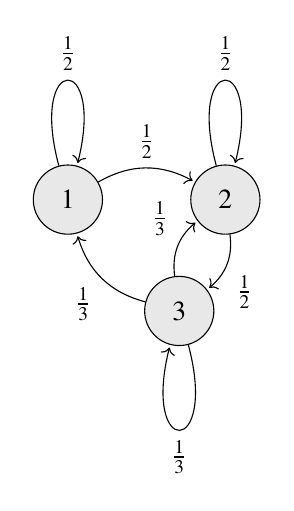
\begin{tikzpicture}[shorten >=1pt,node distance=2cm, scale =3, auto]
			\tikzstyle{every state}=[fill={rgb:black,1;white,10}]
			
			\node[state]   (q_1)                          {$1$};
			\node[state]   (q_2)  [right of=q_1]          {$2$};
			\node[state]   (q_3)  [below right of=q_1]          {$3$};
			
			\path[->]
			(q_1) edge [loop above] node {$\frac{1}{2}$}    (   )
			edge [bend left]  node {$\frac{1}{2}$}    (q_2)
			(q_2) edge [bend left]  node {$\frac{1}{2}$}    (q_3)
			edge [loop above] node {$\frac{1}{2}$}    ()
			(q_3) edge [bend left]  node {$\frac{1}{3}$}    (q_2)
			edge [bend left]  node {$\frac{1}{3}$}    (q_1)
			edge [loop below] node {$\frac{1}{3}$}    ();
		\end{tikzpicture}$
		
		\\  
		&\\
		&\\
		\hline
		\multirow{3}{*}{Checking whether the  } & \\
		& Here,\\chain is Irreducible
		& All the states are accessible to one another. \\and Aperiodic
		& $\implies$ They are in the same communication class. So, it is Irreducible.\\
		& \\
		& There exists the non- zero self-transition, which means that the chain \\
		& is Aperiodic.\\
		&\\ 
		& We know that if the Markov Chain is irreducible and aperiodic then \\
		& \qquad \qquad \qquad $\Vec{\pi}_{j} = \lim_{n \to \infty}P\{X_{n} = j\}$, $j = 1,...,N$ \\
		& These are the stationary probabilities. \\
		&\\
		\hline
		\multirow{3}{*}{Finding the Stationary} & \\
		& Stationary Probability can be represented as\\Probability Distributions
		& \qquad \qquad \qquad $\Vec{\pi} = \Vec{\pi} \vec{P}$\\
		& \\
		& \qquad $\implies$ $\myvec{v_{1}&&v_{2}&&v_{3}} = \myvec{v_{1}&&v_{2}&&v_{3}}\vec{P}$ \\
		& \\
		& Equating the above equation we get \\
		& \\
		& \qquad \qquad \qquad $\frac{1}{2}v_{1}-\frac{1}{3}v_{3} = 0$ $\label{eq:solutions/2018/dec/106/eq}$\\
		& \\
		& \qquad \qquad \qquad $\frac{1}{2}v_{1}-\frac{1}{2}v_{2} + \frac{1}{3}v_{3} = 0$\\
		& \\
		& \qquad \qquad \qquad $\frac{1}{2}v_{2}-\frac{2}{3}v_{3} = 0$\\
		& \\\
		& We see that summation of second and the third equation gives us the \\
		& first equation only. \\
		& And we know that the probability distribution will sum up to 1. \\
		& \\
		& \qquad \qquad \qquad $v_{1}+v_{2}+v_{3} = 1$ \\
		& \\
		& Therefore, we get the equation form as \\
		& \\
		& \qquad \qquad \qquad $\myvec{1&1&1\\\frac{1}{2}&0&\frac{-1}{3}\\\frac{1}{2}&\frac{-1}{2}&\frac{1}{3}}\myvec{v_{1}\\v_{2}\\v_{3}} = \myvec{1\\0\\0}$ \\
		& \\
		\hline
		\multirow{3}{*}{Solving the linear} & \\
		& The above linear equation can be solved using Gauss-Jordan method as\\equtions
		& \\
		& \qquad \qquad \qquad $\myvec{1&1&1&\vrule&1\\\frac{1}{2}&0&\frac{-1}{3}&\vrule&0\\\frac{1}{2}&\frac{-1}{2}&\frac{1}{3}&\vrule&0}$\\
		& \\
		& \qquad $\xleftrightarrow[]{R_2 \leftarrow R_2 - \frac{1}{2}R_1}$
		$\myvec{1&1&1&\vrule&1\\0&\frac{-1}{2}&\frac{-5}{6}&\vrule&\frac{-1}{2}\\\frac{1}{2}&\frac{-1}{2}&\frac{1}{3}&\vrule&0}$\\
		&\\
		& \qquad $\xleftrightarrow[]{R_3 \leftarrow R_3 - \frac{1}{2}R_1}$
		$\myvec{1&1&1&\vrule&1\\0&\frac{-1}{2}&\frac{-5}{6}&\vrule&\frac{-1}{2}\\0&-1&\frac{-1}{6}&\vrule&\frac{-1}{2}}$\\
		&\\
		& \qquad $\xleftrightarrow[]{R_2 \leftarrow \frac{-1}{2}R_2}$
		$\myvec{1&1&1&\vrule&1\\0&1&\frac{5}{3}&\vrule&1\\0&-1&\frac{-1}{6}&\vrule&\frac{-1}{2}}$\\
		&\\
		& \qquad $\xleftrightarrow[]{R_3 \leftarrow R_3 + R_2}$
		$\myvec{1&1&1&\vrule&1\\0&1&\frac{5}{3}&\vrule&1\\0&0&\frac{3}{2}&\vrule&\frac{1}{2}}$\\
		&\\
		& \qquad $\xleftrightarrow[]{R_3 \leftarrow \frac{3}{2}R_3}$
		$\myvec{1&1&1&\vrule&1\\0&1&\frac{5}{3}&\vrule&1\\0&0&1&\vrule&\frac{1}{3}}$\\
		&\\
		& \qquad $\xleftrightarrow[]{R_2 \leftarrow R_2 - \frac{5}{3}R_3}$
		$\myvec{1&1&1&\vrule&1\\0&1&0&\vrule&\frac{4}{9}\\0&0&1&\vrule&\frac{1}{3}}$\\
		&\\
		& \qquad $\xleftrightarrow[]{R_1 \leftarrow R_1 - R_3}$
		$\myvec{1&1&0&\vrule&\frac{2}{3}\\0&1&0&\vrule&\frac{4}{9}\\0&0&1&\vrule&\frac{1}{3}}$\\
		&\\
		& \qquad $\xleftrightarrow[]{R_1 \leftarrow R_1 - R_2}$
		$\myvec{1&0&0&\vrule&\frac{2}{9}\\0&1&0&\vrule&\frac{4}{9}\\0&0&1&\vrule&\frac{1}{3}}$\\
		&\\
		& $\therefore$, stationary probability distribution $\pi$ is given by \\
		& \qquad \qquad $\pi = \myvec{\frac{2}{9} & \frac{4}{9} & \frac{1}{3}}$ \\
		& \\
		\hline
		\multirow{3}{*}{Observations} & \\
		
		
		& Since the given transition probability matrix $\vec{P}$ is irreducible and aperiodic, \\
		& then $\lim_{n \to \infty} \vec{P}^{n}$ converges to a matrix with all rows identical and equal to $\vec{\pi}$. \\
		& \\
		& We were able to find $\vec{\pi}$ as $\myvec{\frac{2}{9} & \frac{4}{9} & \frac{1}{3}}$ \\
		& \\
		& $\lim_{n \to \infty} \vec{P}^{n} = \myvec{\frac{2}{9}&\frac{4}{9}&\frac{1}{3}\\\frac{2}{9}&\frac{4}{9}&\frac{1}{3}\\\frac{2}{9}&\frac{4}{9}&\frac{1}{3}}$\\
		& \\
		& From the above matrix, we get \\
		& \\
		& $\lim_{n \to \infty} \vec{P}^{n}_{11} = \frac{2}{9}$ \\
		&\\
		& $\lim_{n \to \infty} \vec{P}^{n}_{21} = \frac{2}{9}$ \\
		&\\
		& $\lim_{n \to \infty} \vec{P}^{n}_{32} = \frac{4}{9}$ \\
		&\\
		& $\lim_{n \to \infty} \vec{P}^{n}_{13} = \frac{1}{3}$ \\
		&\\
		\hline
		\multirow{3}{*}{Conclusion} & \\
		& From our observation we see that \\
		&\\
		& Options 1) and 4) are True.\\
		& \\
		\hline
\caption{}
\label{eq:solutions/2018/dec/106/table1}
	\end{longtable}
\twocolumn

\end{enumerate}

\section{December 2017}
\renewcommand{\theequation}{\theenumi}
\renewcommand{\thefigure}{\theenumi}
\begin{enumerate}[label=\thesection.\arabic*.,ref=\thesection.\theenumi]
\numberwithin{equation}{enumi}
\numberwithin{figure}{enumi}
\numberwithin{table}{enumi}

\item Consider the subspaces $W_1$ and $W_2$ of $\mathbb{R}^3$ given by
\begin{align}
W_1 &= \cbrak{\vec{x} \in \mathbb{R}^3: \myvec{1 & 1 & 1}\vec{x} = 0}
\label{eq:solutions/2018/dec/27/eq:1}
\\
W_2 &= \cbrak{\vec{x} \in \mathbb{R}^3: \myvec{1 & -1 & 1}\vec{x} = 0}.
\label{eq:solutions/2018/dec/27/eq:2}
\end{align}
If $W \subseteq \mathbb{R}^3$, such that 
\begin{enumerate}
\item $W \cap W_2 =$ span $\cbrak{\myvec{0\\1\\1}}$
\label{eq:solutions/2018/dec/27/eq:3}
\item $\cbrak{W \cap W_1} \perp \cbrak{W \cap W_2}$, 
\label{eq:solutions/2018/dec/27/eq:4}
\end{enumerate}
then 
\begin{enumerate}
\item $W =$ span $\cbrak{\myvec{0\\1\\-1},\myvec{0\\1\\1}}$
\item $W =$ span $\cbrak{\myvec{1\\0\\-1},\myvec{0\\1\\-1}}$
\item $W =$ span $\cbrak{\myvec{1\\0\\-1},\myvec{0\\1\\1}}$
\item $W =$ span $\cbrak{\myvec{1\\0\\-1},\myvec{1\\0\\1}}$
\end{enumerate}
\solution
See Tables \ref{eq:solutions/2018/dec/106/table0} and \ref{eq:solutions/2018/dec/106/table1}


\onecolumn
	\begin{longtable}{|l|l|}
		\hline
		\multirow{3}{*}{Irreducible Markov Chain} 
		& \\
		& A Markov chain is $\textbf{irreducible}$ if all the states communicate with each other,\\
		& i.e., if there is only one communication class.\\
		&\\
		\hline
		\multirow{3}{*}{Aperiodic Markov Chain} & \\
		& If there is a self-transition in the chain ($p^{ii}>0$ for some i), then the chain is\\
		& called as $\textbf{aperiodic}$\\
		& \\
		\hline
		\multirow{3}{*}{Stationary Distribution} & \\
		& A stationary distribution of a Markov chain is a probability distribution that\\
		& remains unchanged in the Markov chain as time progresses. Typically, it is\\
		& represented as a row vector $\Vec{\pi}$ whose entries are probabilities summing to 1,\\ 
		& and given transition matrix $\textbf{P}$, it satisfies\\
		& \\
		&  \qquad \qquad  \qquad$\Vec{\pi} = \Vec{\pi} \textbf{P}$\\
		& \\
		\hline
\caption{}
\label{eq:solutions/2018/dec/106/table0}
	\end{longtable}
	\begin{longtable}{|l|l|}
		\hline
		\multirow{3}{*}{Drawing Transition diagram} 
		& \\
		& 
		
		$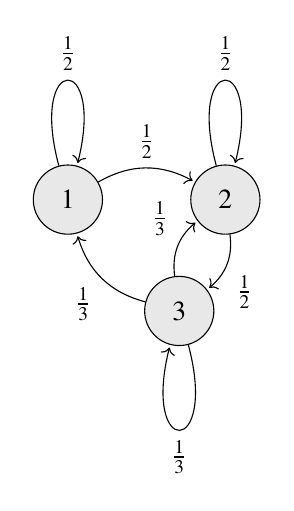
\begin{tikzpicture}[shorten >=1pt,node distance=2cm, scale =3, auto]
			\tikzstyle{every state}=[fill={rgb:black,1;white,10}]
			
			\node[state]   (q_1)                          {$1$};
			\node[state]   (q_2)  [right of=q_1]          {$2$};
			\node[state]   (q_3)  [below right of=q_1]          {$3$};
			
			\path[->]
			(q_1) edge [loop above] node {$\frac{1}{2}$}    (   )
			edge [bend left]  node {$\frac{1}{2}$}    (q_2)
			(q_2) edge [bend left]  node {$\frac{1}{2}$}    (q_3)
			edge [loop above] node {$\frac{1}{2}$}    ()
			(q_3) edge [bend left]  node {$\frac{1}{3}$}    (q_2)
			edge [bend left]  node {$\frac{1}{3}$}    (q_1)
			edge [loop below] node {$\frac{1}{3}$}    ();
		\end{tikzpicture}$
		
		\\  
		&\\
		&\\
		\hline
		\multirow{3}{*}{Checking whether the  } & \\
		& Here,\\chain is Irreducible
		& All the states are accessible to one another. \\and Aperiodic
		& $\implies$ They are in the same communication class. So, it is Irreducible.\\
		& \\
		& There exists the non- zero self-transition, which means that the chain \\
		& is Aperiodic.\\
		&\\ 
		& We know that if the Markov Chain is irreducible and aperiodic then \\
		& \qquad \qquad \qquad $\Vec{\pi}_{j} = \lim_{n \to \infty}P\{X_{n} = j\}$, $j = 1,...,N$ \\
		& These are the stationary probabilities. \\
		&\\
		\hline
		\multirow{3}{*}{Finding the Stationary} & \\
		& Stationary Probability can be represented as\\Probability Distributions
		& \qquad \qquad \qquad $\Vec{\pi} = \Vec{\pi} \vec{P}$\\
		& \\
		& \qquad $\implies$ $\myvec{v_{1}&&v_{2}&&v_{3}} = \myvec{v_{1}&&v_{2}&&v_{3}}\vec{P}$ \\
		& \\
		& Equating the above equation we get \\
		& \\
		& \qquad \qquad \qquad $\frac{1}{2}v_{1}-\frac{1}{3}v_{3} = 0$ $\label{eq:solutions/2018/dec/106/eq}$\\
		& \\
		& \qquad \qquad \qquad $\frac{1}{2}v_{1}-\frac{1}{2}v_{2} + \frac{1}{3}v_{3} = 0$\\
		& \\
		& \qquad \qquad \qquad $\frac{1}{2}v_{2}-\frac{2}{3}v_{3} = 0$\\
		& \\\
		& We see that summation of second and the third equation gives us the \\
		& first equation only. \\
		& And we know that the probability distribution will sum up to 1. \\
		& \\
		& \qquad \qquad \qquad $v_{1}+v_{2}+v_{3} = 1$ \\
		& \\
		& Therefore, we get the equation form as \\
		& \\
		& \qquad \qquad \qquad $\myvec{1&1&1\\\frac{1}{2}&0&\frac{-1}{3}\\\frac{1}{2}&\frac{-1}{2}&\frac{1}{3}}\myvec{v_{1}\\v_{2}\\v_{3}} = \myvec{1\\0\\0}$ \\
		& \\
		\hline
		\multirow{3}{*}{Solving the linear} & \\
		& The above linear equation can be solved using Gauss-Jordan method as\\equtions
		& \\
		& \qquad \qquad \qquad $\myvec{1&1&1&\vrule&1\\\frac{1}{2}&0&\frac{-1}{3}&\vrule&0\\\frac{1}{2}&\frac{-1}{2}&\frac{1}{3}&\vrule&0}$\\
		& \\
		& \qquad $\xleftrightarrow[]{R_2 \leftarrow R_2 - \frac{1}{2}R_1}$
		$\myvec{1&1&1&\vrule&1\\0&\frac{-1}{2}&\frac{-5}{6}&\vrule&\frac{-1}{2}\\\frac{1}{2}&\frac{-1}{2}&\frac{1}{3}&\vrule&0}$\\
		&\\
		& \qquad $\xleftrightarrow[]{R_3 \leftarrow R_3 - \frac{1}{2}R_1}$
		$\myvec{1&1&1&\vrule&1\\0&\frac{-1}{2}&\frac{-5}{6}&\vrule&\frac{-1}{2}\\0&-1&\frac{-1}{6}&\vrule&\frac{-1}{2}}$\\
		&\\
		& \qquad $\xleftrightarrow[]{R_2 \leftarrow \frac{-1}{2}R_2}$
		$\myvec{1&1&1&\vrule&1\\0&1&\frac{5}{3}&\vrule&1\\0&-1&\frac{-1}{6}&\vrule&\frac{-1}{2}}$\\
		&\\
		& \qquad $\xleftrightarrow[]{R_3 \leftarrow R_3 + R_2}$
		$\myvec{1&1&1&\vrule&1\\0&1&\frac{5}{3}&\vrule&1\\0&0&\frac{3}{2}&\vrule&\frac{1}{2}}$\\
		&\\
		& \qquad $\xleftrightarrow[]{R_3 \leftarrow \frac{3}{2}R_3}$
		$\myvec{1&1&1&\vrule&1\\0&1&\frac{5}{3}&\vrule&1\\0&0&1&\vrule&\frac{1}{3}}$\\
		&\\
		& \qquad $\xleftrightarrow[]{R_2 \leftarrow R_2 - \frac{5}{3}R_3}$
		$\myvec{1&1&1&\vrule&1\\0&1&0&\vrule&\frac{4}{9}\\0&0&1&\vrule&\frac{1}{3}}$\\
		&\\
		& \qquad $\xleftrightarrow[]{R_1 \leftarrow R_1 - R_3}$
		$\myvec{1&1&0&\vrule&\frac{2}{3}\\0&1&0&\vrule&\frac{4}{9}\\0&0&1&\vrule&\frac{1}{3}}$\\
		&\\
		& \qquad $\xleftrightarrow[]{R_1 \leftarrow R_1 - R_2}$
		$\myvec{1&0&0&\vrule&\frac{2}{9}\\0&1&0&\vrule&\frac{4}{9}\\0&0&1&\vrule&\frac{1}{3}}$\\
		&\\
		& $\therefore$, stationary probability distribution $\pi$ is given by \\
		& \qquad \qquad $\pi = \myvec{\frac{2}{9} & \frac{4}{9} & \frac{1}{3}}$ \\
		& \\
		\hline
		\multirow{3}{*}{Observations} & \\
		
		
		& Since the given transition probability matrix $\vec{P}$ is irreducible and aperiodic, \\
		& then $\lim_{n \to \infty} \vec{P}^{n}$ converges to a matrix with all rows identical and equal to $\vec{\pi}$. \\
		& \\
		& We were able to find $\vec{\pi}$ as $\myvec{\frac{2}{9} & \frac{4}{9} & \frac{1}{3}}$ \\
		& \\
		& $\lim_{n \to \infty} \vec{P}^{n} = \myvec{\frac{2}{9}&\frac{4}{9}&\frac{1}{3}\\\frac{2}{9}&\frac{4}{9}&\frac{1}{3}\\\frac{2}{9}&\frac{4}{9}&\frac{1}{3}}$\\
		& \\
		& From the above matrix, we get \\
		& \\
		& $\lim_{n \to \infty} \vec{P}^{n}_{11} = \frac{2}{9}$ \\
		&\\
		& $\lim_{n \to \infty} \vec{P}^{n}_{21} = \frac{2}{9}$ \\
		&\\
		& $\lim_{n \to \infty} \vec{P}^{n}_{32} = \frac{4}{9}$ \\
		&\\
		& $\lim_{n \to \infty} \vec{P}^{n}_{13} = \frac{1}{3}$ \\
		&\\
		\hline
		\multirow{3}{*}{Conclusion} & \\
		& From our observation we see that \\
		&\\
		& Options 1) and 4) are True.\\
		& \\
		\hline
\caption{}
\label{eq:solutions/2018/dec/106/table1}
	\end{longtable}
\twocolumn

%
\item Let
\begin{align}
C = \cbrak{\myvec{1 \\ 2},\myvec{2 \\ 1}}
\end{align}
be a basis of $\mathbb{R}^2$ and 
\begin{align}
T\myvec{x\\y} = \myvec{x+y \\ x-2y}.
\end{align}
If $T\sbrak{C}$ represents the matrix of $T$ with respect to the basis C then
which among the following is true?
\begin{enumerate}
\item $T\sbrak{C} = \myvec{-3 & -2\\3 & 1}$
\item $T\sbrak{C} = \myvec{3 & -2\\-3 & 1}$
\item $T\sbrak{C} = \myvec{-3 & -1\\3 & 2}$
\item $T\sbrak{C} = \myvec{3 & -1\\-3 & 2}$
\end{enumerate}
\solution
See Tables \ref{eq:solutions/2018/dec/106/table0} and \ref{eq:solutions/2018/dec/106/table1}


\onecolumn
	\begin{longtable}{|l|l|}
		\hline
		\multirow{3}{*}{Irreducible Markov Chain} 
		& \\
		& A Markov chain is $\textbf{irreducible}$ if all the states communicate with each other,\\
		& i.e., if there is only one communication class.\\
		&\\
		\hline
		\multirow{3}{*}{Aperiodic Markov Chain} & \\
		& If there is a self-transition in the chain ($p^{ii}>0$ for some i), then the chain is\\
		& called as $\textbf{aperiodic}$\\
		& \\
		\hline
		\multirow{3}{*}{Stationary Distribution} & \\
		& A stationary distribution of a Markov chain is a probability distribution that\\
		& remains unchanged in the Markov chain as time progresses. Typically, it is\\
		& represented as a row vector $\Vec{\pi}$ whose entries are probabilities summing to 1,\\ 
		& and given transition matrix $\textbf{P}$, it satisfies\\
		& \\
		&  \qquad \qquad  \qquad$\Vec{\pi} = \Vec{\pi} \textbf{P}$\\
		& \\
		\hline
\caption{}
\label{eq:solutions/2018/dec/106/table0}
	\end{longtable}
	\begin{longtable}{|l|l|}
		\hline
		\multirow{3}{*}{Drawing Transition diagram} 
		& \\
		& 
		
		$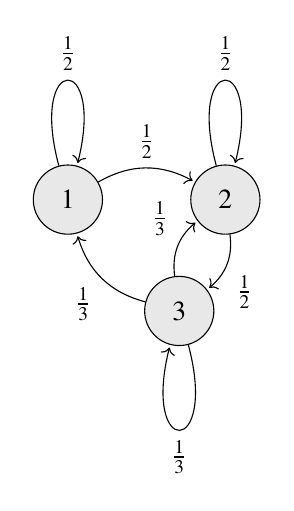
\begin{tikzpicture}[shorten >=1pt,node distance=2cm, scale =3, auto]
			\tikzstyle{every state}=[fill={rgb:black,1;white,10}]
			
			\node[state]   (q_1)                          {$1$};
			\node[state]   (q_2)  [right of=q_1]          {$2$};
			\node[state]   (q_3)  [below right of=q_1]          {$3$};
			
			\path[->]
			(q_1) edge [loop above] node {$\frac{1}{2}$}    (   )
			edge [bend left]  node {$\frac{1}{2}$}    (q_2)
			(q_2) edge [bend left]  node {$\frac{1}{2}$}    (q_3)
			edge [loop above] node {$\frac{1}{2}$}    ()
			(q_3) edge [bend left]  node {$\frac{1}{3}$}    (q_2)
			edge [bend left]  node {$\frac{1}{3}$}    (q_1)
			edge [loop below] node {$\frac{1}{3}$}    ();
		\end{tikzpicture}$
		
		\\  
		&\\
		&\\
		\hline
		\multirow{3}{*}{Checking whether the  } & \\
		& Here,\\chain is Irreducible
		& All the states are accessible to one another. \\and Aperiodic
		& $\implies$ They are in the same communication class. So, it is Irreducible.\\
		& \\
		& There exists the non- zero self-transition, which means that the chain \\
		& is Aperiodic.\\
		&\\ 
		& We know that if the Markov Chain is irreducible and aperiodic then \\
		& \qquad \qquad \qquad $\Vec{\pi}_{j} = \lim_{n \to \infty}P\{X_{n} = j\}$, $j = 1,...,N$ \\
		& These are the stationary probabilities. \\
		&\\
		\hline
		\multirow{3}{*}{Finding the Stationary} & \\
		& Stationary Probability can be represented as\\Probability Distributions
		& \qquad \qquad \qquad $\Vec{\pi} = \Vec{\pi} \vec{P}$\\
		& \\
		& \qquad $\implies$ $\myvec{v_{1}&&v_{2}&&v_{3}} = \myvec{v_{1}&&v_{2}&&v_{3}}\vec{P}$ \\
		& \\
		& Equating the above equation we get \\
		& \\
		& \qquad \qquad \qquad $\frac{1}{2}v_{1}-\frac{1}{3}v_{3} = 0$ $\label{eq:solutions/2018/dec/106/eq}$\\
		& \\
		& \qquad \qquad \qquad $\frac{1}{2}v_{1}-\frac{1}{2}v_{2} + \frac{1}{3}v_{3} = 0$\\
		& \\
		& \qquad \qquad \qquad $\frac{1}{2}v_{2}-\frac{2}{3}v_{3} = 0$\\
		& \\\
		& We see that summation of second and the third equation gives us the \\
		& first equation only. \\
		& And we know that the probability distribution will sum up to 1. \\
		& \\
		& \qquad \qquad \qquad $v_{1}+v_{2}+v_{3} = 1$ \\
		& \\
		& Therefore, we get the equation form as \\
		& \\
		& \qquad \qquad \qquad $\myvec{1&1&1\\\frac{1}{2}&0&\frac{-1}{3}\\\frac{1}{2}&\frac{-1}{2}&\frac{1}{3}}\myvec{v_{1}\\v_{2}\\v_{3}} = \myvec{1\\0\\0}$ \\
		& \\
		\hline
		\multirow{3}{*}{Solving the linear} & \\
		& The above linear equation can be solved using Gauss-Jordan method as\\equtions
		& \\
		& \qquad \qquad \qquad $\myvec{1&1&1&\vrule&1\\\frac{1}{2}&0&\frac{-1}{3}&\vrule&0\\\frac{1}{2}&\frac{-1}{2}&\frac{1}{3}&\vrule&0}$\\
		& \\
		& \qquad $\xleftrightarrow[]{R_2 \leftarrow R_2 - \frac{1}{2}R_1}$
		$\myvec{1&1&1&\vrule&1\\0&\frac{-1}{2}&\frac{-5}{6}&\vrule&\frac{-1}{2}\\\frac{1}{2}&\frac{-1}{2}&\frac{1}{3}&\vrule&0}$\\
		&\\
		& \qquad $\xleftrightarrow[]{R_3 \leftarrow R_3 - \frac{1}{2}R_1}$
		$\myvec{1&1&1&\vrule&1\\0&\frac{-1}{2}&\frac{-5}{6}&\vrule&\frac{-1}{2}\\0&-1&\frac{-1}{6}&\vrule&\frac{-1}{2}}$\\
		&\\
		& \qquad $\xleftrightarrow[]{R_2 \leftarrow \frac{-1}{2}R_2}$
		$\myvec{1&1&1&\vrule&1\\0&1&\frac{5}{3}&\vrule&1\\0&-1&\frac{-1}{6}&\vrule&\frac{-1}{2}}$\\
		&\\
		& \qquad $\xleftrightarrow[]{R_3 \leftarrow R_3 + R_2}$
		$\myvec{1&1&1&\vrule&1\\0&1&\frac{5}{3}&\vrule&1\\0&0&\frac{3}{2}&\vrule&\frac{1}{2}}$\\
		&\\
		& \qquad $\xleftrightarrow[]{R_3 \leftarrow \frac{3}{2}R_3}$
		$\myvec{1&1&1&\vrule&1\\0&1&\frac{5}{3}&\vrule&1\\0&0&1&\vrule&\frac{1}{3}}$\\
		&\\
		& \qquad $\xleftrightarrow[]{R_2 \leftarrow R_2 - \frac{5}{3}R_3}$
		$\myvec{1&1&1&\vrule&1\\0&1&0&\vrule&\frac{4}{9}\\0&0&1&\vrule&\frac{1}{3}}$\\
		&\\
		& \qquad $\xleftrightarrow[]{R_1 \leftarrow R_1 - R_3}$
		$\myvec{1&1&0&\vrule&\frac{2}{3}\\0&1&0&\vrule&\frac{4}{9}\\0&0&1&\vrule&\frac{1}{3}}$\\
		&\\
		& \qquad $\xleftrightarrow[]{R_1 \leftarrow R_1 - R_2}$
		$\myvec{1&0&0&\vrule&\frac{2}{9}\\0&1&0&\vrule&\frac{4}{9}\\0&0&1&\vrule&\frac{1}{3}}$\\
		&\\
		& $\therefore$, stationary probability distribution $\pi$ is given by \\
		& \qquad \qquad $\pi = \myvec{\frac{2}{9} & \frac{4}{9} & \frac{1}{3}}$ \\
		& \\
		\hline
		\multirow{3}{*}{Observations} & \\
		
		
		& Since the given transition probability matrix $\vec{P}$ is irreducible and aperiodic, \\
		& then $\lim_{n \to \infty} \vec{P}^{n}$ converges to a matrix with all rows identical and equal to $\vec{\pi}$. \\
		& \\
		& We were able to find $\vec{\pi}$ as $\myvec{\frac{2}{9} & \frac{4}{9} & \frac{1}{3}}$ \\
		& \\
		& $\lim_{n \to \infty} \vec{P}^{n} = \myvec{\frac{2}{9}&\frac{4}{9}&\frac{1}{3}\\\frac{2}{9}&\frac{4}{9}&\frac{1}{3}\\\frac{2}{9}&\frac{4}{9}&\frac{1}{3}}$\\
		& \\
		& From the above matrix, we get \\
		& \\
		& $\lim_{n \to \infty} \vec{P}^{n}_{11} = \frac{2}{9}$ \\
		&\\
		& $\lim_{n \to \infty} \vec{P}^{n}_{21} = \frac{2}{9}$ \\
		&\\
		& $\lim_{n \to \infty} \vec{P}^{n}_{32} = \frac{4}{9}$ \\
		&\\
		& $\lim_{n \to \infty} \vec{P}^{n}_{13} = \frac{1}{3}$ \\
		&\\
		\hline
		\multirow{3}{*}{Conclusion} & \\
		& From our observation we see that \\
		&\\
		& Options 1) and 4) are True.\\
		& \\
		\hline
\caption{}
\label{eq:solutions/2018/dec/106/table1}
	\end{longtable}
\twocolumn

\item Let $W_1 = \cbrak{\vec{x} \in \mathbb{R}^4:}$
\begin{align}
 \myvec{1 & 1 & 1 & 0}\vec{x} = 0
\\
 \myvec{0 & 2 & 0 & 1}\vec{x} = 0
\\
 \myvec{2 & 0 & 2 & -1}\vec{x} = 0
\end{align}
and
$W_2 = \cbrak{\vec{x} \in \mathbb{R}^4:}$
\begin{align}
 \myvec{1 & 1 & 0 & 1}\vec{x} &= 0
\\
 \myvec{1 & 0 & 1 & -2}\vec{x} &= 0
\\
 \myvec{0 & 1 & 0 & -1}\vec{x} &= 0.
\end{align}
Then which among the following is true?
\begin{enumerate}
\item $\text{dim}\brak{W_1} = 1$
\item $\text{dim}\brak{W_2} = 2$
\item $\text{dim}\brak{W_1 \cap W_2} = 1$
\item $\text{dim}\brak{W_1+W_2} = 3$
\end{enumerate}
%
\item Let $A$ be an $n \times n$ complex matrix.  Assume that $A$ is self-adjoint and let $B$ denote the inverse of $A + \j I$. Then all eigenvalues of $\brak{A-\j I}B$ are 
\begin{enumerate}
\item purely imaginary
\item of modulus one
\item real
\item of modulus less than one
\end{enumerate}  
%
\item Let $\cbrak{u_1,u_2,\dots, u_n}$ be an orthonormal basis of $\mathbb{C}^n$ as column vectors.Let 
\begin{align}
\vec{M} &= \myvec{\vec{u}_1 & \vec{u}_2 & \dots & \vec{u}_k},
\\
\vec{N} &= \myvec{\vec{u}_{k+1} & \vec{u}_{k+2} & \dots & \vec{u}_n}
\end{align}
%
and $\vec{P}$ be the diagonal $k \times k$ matrix with diagonal entries $\alpha_1,\alpha_2, \dots, \alpha_k \in \mathbb{R}$.  Then which of the following is true?
\begin{enumerate}
\item rank$\brak{\vec{M}\vec{P}\vec{M}^*} = k$ whenever $\alpha_i \ne \alpha_j, 1 \le i, j \le k$.
\item tr$\brak{\vec{M}\vec{P}\vec{M}^*} = \sum_{i=1}^{k}\alpha_i$
\item rank$\brak{\vec{M}^*\vec{N}} = \min\brak{k,n-k}$
\item rank$\brak{\vec{M}\vec{M}^*+\vec{N}\vec{N}^*}  < n$.
\end{enumerate}  
%
\solution
See Tables \ref{eq:solutions/2018/dec/106/table0} and \ref{eq:solutions/2018/dec/106/table1}


\onecolumn
	\begin{longtable}{|l|l|}
		\hline
		\multirow{3}{*}{Irreducible Markov Chain} 
		& \\
		& A Markov chain is $\textbf{irreducible}$ if all the states communicate with each other,\\
		& i.e., if there is only one communication class.\\
		&\\
		\hline
		\multirow{3}{*}{Aperiodic Markov Chain} & \\
		& If there is a self-transition in the chain ($p^{ii}>0$ for some i), then the chain is\\
		& called as $\textbf{aperiodic}$\\
		& \\
		\hline
		\multirow{3}{*}{Stationary Distribution} & \\
		& A stationary distribution of a Markov chain is a probability distribution that\\
		& remains unchanged in the Markov chain as time progresses. Typically, it is\\
		& represented as a row vector $\Vec{\pi}$ whose entries are probabilities summing to 1,\\ 
		& and given transition matrix $\textbf{P}$, it satisfies\\
		& \\
		&  \qquad \qquad  \qquad$\Vec{\pi} = \Vec{\pi} \textbf{P}$\\
		& \\
		\hline
\caption{}
\label{eq:solutions/2018/dec/106/table0}
	\end{longtable}
	\begin{longtable}{|l|l|}
		\hline
		\multirow{3}{*}{Drawing Transition diagram} 
		& \\
		& 
		
		$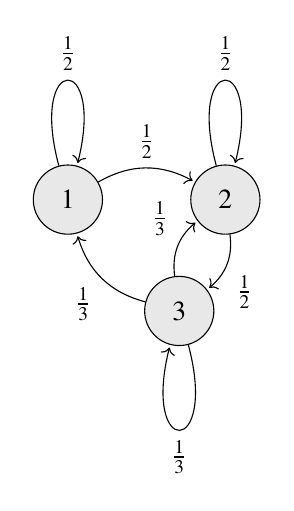
\begin{tikzpicture}[shorten >=1pt,node distance=2cm, scale =3, auto]
			\tikzstyle{every state}=[fill={rgb:black,1;white,10}]
			
			\node[state]   (q_1)                          {$1$};
			\node[state]   (q_2)  [right of=q_1]          {$2$};
			\node[state]   (q_3)  [below right of=q_1]          {$3$};
			
			\path[->]
			(q_1) edge [loop above] node {$\frac{1}{2}$}    (   )
			edge [bend left]  node {$\frac{1}{2}$}    (q_2)
			(q_2) edge [bend left]  node {$\frac{1}{2}$}    (q_3)
			edge [loop above] node {$\frac{1}{2}$}    ()
			(q_3) edge [bend left]  node {$\frac{1}{3}$}    (q_2)
			edge [bend left]  node {$\frac{1}{3}$}    (q_1)
			edge [loop below] node {$\frac{1}{3}$}    ();
		\end{tikzpicture}$
		
		\\  
		&\\
		&\\
		\hline
		\multirow{3}{*}{Checking whether the  } & \\
		& Here,\\chain is Irreducible
		& All the states are accessible to one another. \\and Aperiodic
		& $\implies$ They are in the same communication class. So, it is Irreducible.\\
		& \\
		& There exists the non- zero self-transition, which means that the chain \\
		& is Aperiodic.\\
		&\\ 
		& We know that if the Markov Chain is irreducible and aperiodic then \\
		& \qquad \qquad \qquad $\Vec{\pi}_{j} = \lim_{n \to \infty}P\{X_{n} = j\}$, $j = 1,...,N$ \\
		& These are the stationary probabilities. \\
		&\\
		\hline
		\multirow{3}{*}{Finding the Stationary} & \\
		& Stationary Probability can be represented as\\Probability Distributions
		& \qquad \qquad \qquad $\Vec{\pi} = \Vec{\pi} \vec{P}$\\
		& \\
		& \qquad $\implies$ $\myvec{v_{1}&&v_{2}&&v_{3}} = \myvec{v_{1}&&v_{2}&&v_{3}}\vec{P}$ \\
		& \\
		& Equating the above equation we get \\
		& \\
		& \qquad \qquad \qquad $\frac{1}{2}v_{1}-\frac{1}{3}v_{3} = 0$ $\label{eq:solutions/2018/dec/106/eq}$\\
		& \\
		& \qquad \qquad \qquad $\frac{1}{2}v_{1}-\frac{1}{2}v_{2} + \frac{1}{3}v_{3} = 0$\\
		& \\
		& \qquad \qquad \qquad $\frac{1}{2}v_{2}-\frac{2}{3}v_{3} = 0$\\
		& \\\
		& We see that summation of second and the third equation gives us the \\
		& first equation only. \\
		& And we know that the probability distribution will sum up to 1. \\
		& \\
		& \qquad \qquad \qquad $v_{1}+v_{2}+v_{3} = 1$ \\
		& \\
		& Therefore, we get the equation form as \\
		& \\
		& \qquad \qquad \qquad $\myvec{1&1&1\\\frac{1}{2}&0&\frac{-1}{3}\\\frac{1}{2}&\frac{-1}{2}&\frac{1}{3}}\myvec{v_{1}\\v_{2}\\v_{3}} = \myvec{1\\0\\0}$ \\
		& \\
		\hline
		\multirow{3}{*}{Solving the linear} & \\
		& The above linear equation can be solved using Gauss-Jordan method as\\equtions
		& \\
		& \qquad \qquad \qquad $\myvec{1&1&1&\vrule&1\\\frac{1}{2}&0&\frac{-1}{3}&\vrule&0\\\frac{1}{2}&\frac{-1}{2}&\frac{1}{3}&\vrule&0}$\\
		& \\
		& \qquad $\xleftrightarrow[]{R_2 \leftarrow R_2 - \frac{1}{2}R_1}$
		$\myvec{1&1&1&\vrule&1\\0&\frac{-1}{2}&\frac{-5}{6}&\vrule&\frac{-1}{2}\\\frac{1}{2}&\frac{-1}{2}&\frac{1}{3}&\vrule&0}$\\
		&\\
		& \qquad $\xleftrightarrow[]{R_3 \leftarrow R_3 - \frac{1}{2}R_1}$
		$\myvec{1&1&1&\vrule&1\\0&\frac{-1}{2}&\frac{-5}{6}&\vrule&\frac{-1}{2}\\0&-1&\frac{-1}{6}&\vrule&\frac{-1}{2}}$\\
		&\\
		& \qquad $\xleftrightarrow[]{R_2 \leftarrow \frac{-1}{2}R_2}$
		$\myvec{1&1&1&\vrule&1\\0&1&\frac{5}{3}&\vrule&1\\0&-1&\frac{-1}{6}&\vrule&\frac{-1}{2}}$\\
		&\\
		& \qquad $\xleftrightarrow[]{R_3 \leftarrow R_3 + R_2}$
		$\myvec{1&1&1&\vrule&1\\0&1&\frac{5}{3}&\vrule&1\\0&0&\frac{3}{2}&\vrule&\frac{1}{2}}$\\
		&\\
		& \qquad $\xleftrightarrow[]{R_3 \leftarrow \frac{3}{2}R_3}$
		$\myvec{1&1&1&\vrule&1\\0&1&\frac{5}{3}&\vrule&1\\0&0&1&\vrule&\frac{1}{3}}$\\
		&\\
		& \qquad $\xleftrightarrow[]{R_2 \leftarrow R_2 - \frac{5}{3}R_3}$
		$\myvec{1&1&1&\vrule&1\\0&1&0&\vrule&\frac{4}{9}\\0&0&1&\vrule&\frac{1}{3}}$\\
		&\\
		& \qquad $\xleftrightarrow[]{R_1 \leftarrow R_1 - R_3}$
		$\myvec{1&1&0&\vrule&\frac{2}{3}\\0&1&0&\vrule&\frac{4}{9}\\0&0&1&\vrule&\frac{1}{3}}$\\
		&\\
		& \qquad $\xleftrightarrow[]{R_1 \leftarrow R_1 - R_2}$
		$\myvec{1&0&0&\vrule&\frac{2}{9}\\0&1&0&\vrule&\frac{4}{9}\\0&0&1&\vrule&\frac{1}{3}}$\\
		&\\
		& $\therefore$, stationary probability distribution $\pi$ is given by \\
		& \qquad \qquad $\pi = \myvec{\frac{2}{9} & \frac{4}{9} & \frac{1}{3}}$ \\
		& \\
		\hline
		\multirow{3}{*}{Observations} & \\
		
		
		& Since the given transition probability matrix $\vec{P}$ is irreducible and aperiodic, \\
		& then $\lim_{n \to \infty} \vec{P}^{n}$ converges to a matrix with all rows identical and equal to $\vec{\pi}$. \\
		& \\
		& We were able to find $\vec{\pi}$ as $\myvec{\frac{2}{9} & \frac{4}{9} & \frac{1}{3}}$ \\
		& \\
		& $\lim_{n \to \infty} \vec{P}^{n} = \myvec{\frac{2}{9}&\frac{4}{9}&\frac{1}{3}\\\frac{2}{9}&\frac{4}{9}&\frac{1}{3}\\\frac{2}{9}&\frac{4}{9}&\frac{1}{3}}$\\
		& \\
		& From the above matrix, we get \\
		& \\
		& $\lim_{n \to \infty} \vec{P}^{n}_{11} = \frac{2}{9}$ \\
		&\\
		& $\lim_{n \to \infty} \vec{P}^{n}_{21} = \frac{2}{9}$ \\
		&\\
		& $\lim_{n \to \infty} \vec{P}^{n}_{32} = \frac{4}{9}$ \\
		&\\
		& $\lim_{n \to \infty} \vec{P}^{n}_{13} = \frac{1}{3}$ \\
		&\\
		\hline
		\multirow{3}{*}{Conclusion} & \\
		& From our observation we see that \\
		&\\
		& Options 1) and 4) are True.\\
		& \\
		\hline
\caption{}
\label{eq:solutions/2018/dec/106/table1}
	\end{longtable}
\twocolumn

\item Let $B: \mathbb{R} \times \mathbb{R} \xrightarrow[]{} \mathbb{R}$ be the function $B(a,b) = ab$. Which of the following is true-
\begin{enumerate}
\item{$B$ is a linear transformation}
\item{$B$ is a positive definite bilinear form}
\item{$B$ is symmetric but not positive definite}
\item{$B$ neither linear nor bilinear}
\end{enumerate}
%
\solution
See Tables \ref{eq:solutions/2018/dec/106/table0} and \ref{eq:solutions/2018/dec/106/table1}


\onecolumn
	\begin{longtable}{|l|l|}
		\hline
		\multirow{3}{*}{Irreducible Markov Chain} 
		& \\
		& A Markov chain is $\textbf{irreducible}$ if all the states communicate with each other,\\
		& i.e., if there is only one communication class.\\
		&\\
		\hline
		\multirow{3}{*}{Aperiodic Markov Chain} & \\
		& If there is a self-transition in the chain ($p^{ii}>0$ for some i), then the chain is\\
		& called as $\textbf{aperiodic}$\\
		& \\
		\hline
		\multirow{3}{*}{Stationary Distribution} & \\
		& A stationary distribution of a Markov chain is a probability distribution that\\
		& remains unchanged in the Markov chain as time progresses. Typically, it is\\
		& represented as a row vector $\Vec{\pi}$ whose entries are probabilities summing to 1,\\ 
		& and given transition matrix $\textbf{P}$, it satisfies\\
		& \\
		&  \qquad \qquad  \qquad$\Vec{\pi} = \Vec{\pi} \textbf{P}$\\
		& \\
		\hline
\caption{}
\label{eq:solutions/2018/dec/106/table0}
	\end{longtable}
	\begin{longtable}{|l|l|}
		\hline
		\multirow{3}{*}{Drawing Transition diagram} 
		& \\
		& 
		
		$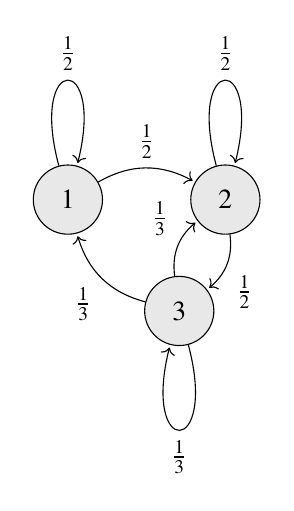
\begin{tikzpicture}[shorten >=1pt,node distance=2cm, scale =3, auto]
			\tikzstyle{every state}=[fill={rgb:black,1;white,10}]
			
			\node[state]   (q_1)                          {$1$};
			\node[state]   (q_2)  [right of=q_1]          {$2$};
			\node[state]   (q_3)  [below right of=q_1]          {$3$};
			
			\path[->]
			(q_1) edge [loop above] node {$\frac{1}{2}$}    (   )
			edge [bend left]  node {$\frac{1}{2}$}    (q_2)
			(q_2) edge [bend left]  node {$\frac{1}{2}$}    (q_3)
			edge [loop above] node {$\frac{1}{2}$}    ()
			(q_3) edge [bend left]  node {$\frac{1}{3}$}    (q_2)
			edge [bend left]  node {$\frac{1}{3}$}    (q_1)
			edge [loop below] node {$\frac{1}{3}$}    ();
		\end{tikzpicture}$
		
		\\  
		&\\
		&\\
		\hline
		\multirow{3}{*}{Checking whether the  } & \\
		& Here,\\chain is Irreducible
		& All the states are accessible to one another. \\and Aperiodic
		& $\implies$ They are in the same communication class. So, it is Irreducible.\\
		& \\
		& There exists the non- zero self-transition, which means that the chain \\
		& is Aperiodic.\\
		&\\ 
		& We know that if the Markov Chain is irreducible and aperiodic then \\
		& \qquad \qquad \qquad $\Vec{\pi}_{j} = \lim_{n \to \infty}P\{X_{n} = j\}$, $j = 1,...,N$ \\
		& These are the stationary probabilities. \\
		&\\
		\hline
		\multirow{3}{*}{Finding the Stationary} & \\
		& Stationary Probability can be represented as\\Probability Distributions
		& \qquad \qquad \qquad $\Vec{\pi} = \Vec{\pi} \vec{P}$\\
		& \\
		& \qquad $\implies$ $\myvec{v_{1}&&v_{2}&&v_{3}} = \myvec{v_{1}&&v_{2}&&v_{3}}\vec{P}$ \\
		& \\
		& Equating the above equation we get \\
		& \\
		& \qquad \qquad \qquad $\frac{1}{2}v_{1}-\frac{1}{3}v_{3} = 0$ $\label{eq:solutions/2018/dec/106/eq}$\\
		& \\
		& \qquad \qquad \qquad $\frac{1}{2}v_{1}-\frac{1}{2}v_{2} + \frac{1}{3}v_{3} = 0$\\
		& \\
		& \qquad \qquad \qquad $\frac{1}{2}v_{2}-\frac{2}{3}v_{3} = 0$\\
		& \\\
		& We see that summation of second and the third equation gives us the \\
		& first equation only. \\
		& And we know that the probability distribution will sum up to 1. \\
		& \\
		& \qquad \qquad \qquad $v_{1}+v_{2}+v_{3} = 1$ \\
		& \\
		& Therefore, we get the equation form as \\
		& \\
		& \qquad \qquad \qquad $\myvec{1&1&1\\\frac{1}{2}&0&\frac{-1}{3}\\\frac{1}{2}&\frac{-1}{2}&\frac{1}{3}}\myvec{v_{1}\\v_{2}\\v_{3}} = \myvec{1\\0\\0}$ \\
		& \\
		\hline
		\multirow{3}{*}{Solving the linear} & \\
		& The above linear equation can be solved using Gauss-Jordan method as\\equtions
		& \\
		& \qquad \qquad \qquad $\myvec{1&1&1&\vrule&1\\\frac{1}{2}&0&\frac{-1}{3}&\vrule&0\\\frac{1}{2}&\frac{-1}{2}&\frac{1}{3}&\vrule&0}$\\
		& \\
		& \qquad $\xleftrightarrow[]{R_2 \leftarrow R_2 - \frac{1}{2}R_1}$
		$\myvec{1&1&1&\vrule&1\\0&\frac{-1}{2}&\frac{-5}{6}&\vrule&\frac{-1}{2}\\\frac{1}{2}&\frac{-1}{2}&\frac{1}{3}&\vrule&0}$\\
		&\\
		& \qquad $\xleftrightarrow[]{R_3 \leftarrow R_3 - \frac{1}{2}R_1}$
		$\myvec{1&1&1&\vrule&1\\0&\frac{-1}{2}&\frac{-5}{6}&\vrule&\frac{-1}{2}\\0&-1&\frac{-1}{6}&\vrule&\frac{-1}{2}}$\\
		&\\
		& \qquad $\xleftrightarrow[]{R_2 \leftarrow \frac{-1}{2}R_2}$
		$\myvec{1&1&1&\vrule&1\\0&1&\frac{5}{3}&\vrule&1\\0&-1&\frac{-1}{6}&\vrule&\frac{-1}{2}}$\\
		&\\
		& \qquad $\xleftrightarrow[]{R_3 \leftarrow R_3 + R_2}$
		$\myvec{1&1&1&\vrule&1\\0&1&\frac{5}{3}&\vrule&1\\0&0&\frac{3}{2}&\vrule&\frac{1}{2}}$\\
		&\\
		& \qquad $\xleftrightarrow[]{R_3 \leftarrow \frac{3}{2}R_3}$
		$\myvec{1&1&1&\vrule&1\\0&1&\frac{5}{3}&\vrule&1\\0&0&1&\vrule&\frac{1}{3}}$\\
		&\\
		& \qquad $\xleftrightarrow[]{R_2 \leftarrow R_2 - \frac{5}{3}R_3}$
		$\myvec{1&1&1&\vrule&1\\0&1&0&\vrule&\frac{4}{9}\\0&0&1&\vrule&\frac{1}{3}}$\\
		&\\
		& \qquad $\xleftrightarrow[]{R_1 \leftarrow R_1 - R_3}$
		$\myvec{1&1&0&\vrule&\frac{2}{3}\\0&1&0&\vrule&\frac{4}{9}\\0&0&1&\vrule&\frac{1}{3}}$\\
		&\\
		& \qquad $\xleftrightarrow[]{R_1 \leftarrow R_1 - R_2}$
		$\myvec{1&0&0&\vrule&\frac{2}{9}\\0&1&0&\vrule&\frac{4}{9}\\0&0&1&\vrule&\frac{1}{3}}$\\
		&\\
		& $\therefore$, stationary probability distribution $\pi$ is given by \\
		& \qquad \qquad $\pi = \myvec{\frac{2}{9} & \frac{4}{9} & \frac{1}{3}}$ \\
		& \\
		\hline
		\multirow{3}{*}{Observations} & \\
		
		
		& Since the given transition probability matrix $\vec{P}$ is irreducible and aperiodic, \\
		& then $\lim_{n \to \infty} \vec{P}^{n}$ converges to a matrix with all rows identical and equal to $\vec{\pi}$. \\
		& \\
		& We were able to find $\vec{\pi}$ as $\myvec{\frac{2}{9} & \frac{4}{9} & \frac{1}{3}}$ \\
		& \\
		& $\lim_{n \to \infty} \vec{P}^{n} = \myvec{\frac{2}{9}&\frac{4}{9}&\frac{1}{3}\\\frac{2}{9}&\frac{4}{9}&\frac{1}{3}\\\frac{2}{9}&\frac{4}{9}&\frac{1}{3}}$\\
		& \\
		& From the above matrix, we get \\
		& \\
		& $\lim_{n \to \infty} \vec{P}^{n}_{11} = \frac{2}{9}$ \\
		&\\
		& $\lim_{n \to \infty} \vec{P}^{n}_{21} = \frac{2}{9}$ \\
		&\\
		& $\lim_{n \to \infty} \vec{P}^{n}_{32} = \frac{4}{9}$ \\
		&\\
		& $\lim_{n \to \infty} \vec{P}^{n}_{13} = \frac{1}{3}$ \\
		&\\
		\hline
		\multirow{3}{*}{Conclusion} & \\
		& From our observation we see that \\
		&\\
		& Options 1) and 4) are True.\\
		& \\
		\hline
\caption{}
\label{eq:solutions/2018/dec/106/table1}
	\end{longtable}
\twocolumn

\item Let $B: \mathbb{R} \times \mathbb{R} \to \mathbb{R}$ be the function
\begin{align}
B(a,b) = ab
\end{align}
Which of the following is true?
\begin{enumerate}
\item $B$ is a linear transformation
\item $B$ is a positive definite bilinear form
\item $B$ is symmetric but not positive definite
\item $B$ is neither linear nor bilinear
\end{enumerate}  
%
\item Let $\vec{A}$ be an invertible real $n \times n$ matrix.  Define a function
\begin{align}
F: \mathbb{R}^n \times \mathbb{R}^n \to \mathbb{R}
\end{align}
by 
\begin{align}
F(\vec{x},\vec{y}) = \brak{F\vec{x}}^T\vec{y}
\end{align}
Let $DF(\vec{x},\vec{y}) $ denote the derivate of $F$ at $(\vec{x},\vec{y}) $ which is 
a linear transformation from 
\begin{align}
\mathbb{R}^n \times \mathbb{R}^n \to \mathbb{R}
\end{align}
%
Then, if 
\begin{enumerate}
\item $\vec{x} \ne 0, DF(\vec{x},\vec{0}) \ne 0$ 
\item $\vec{y} \ne 0, DF(\vec{0},\vec{y}) \ne 0$ 
\item $(\vec{x},\vec{y}) \ne (\vec{0},\vec{0}), DF(\vec{x},\vec{0}) \ne 0$ 
\item $\vec{x} = 0$ or  $\vec{y} = 0, DF(\vec{x},\vec{y}) = 0$ 
\end{enumerate}  
%
\solution
See Tables \ref{eq:solutions/2018/dec/106/table0} and \ref{eq:solutions/2018/dec/106/table1}


\onecolumn
	\begin{longtable}{|l|l|}
		\hline
		\multirow{3}{*}{Irreducible Markov Chain} 
		& \\
		& A Markov chain is $\textbf{irreducible}$ if all the states communicate with each other,\\
		& i.e., if there is only one communication class.\\
		&\\
		\hline
		\multirow{3}{*}{Aperiodic Markov Chain} & \\
		& If there is a self-transition in the chain ($p^{ii}>0$ for some i), then the chain is\\
		& called as $\textbf{aperiodic}$\\
		& \\
		\hline
		\multirow{3}{*}{Stationary Distribution} & \\
		& A stationary distribution of a Markov chain is a probability distribution that\\
		& remains unchanged in the Markov chain as time progresses. Typically, it is\\
		& represented as a row vector $\Vec{\pi}$ whose entries are probabilities summing to 1,\\ 
		& and given transition matrix $\textbf{P}$, it satisfies\\
		& \\
		&  \qquad \qquad  \qquad$\Vec{\pi} = \Vec{\pi} \textbf{P}$\\
		& \\
		\hline
\caption{}
\label{eq:solutions/2018/dec/106/table0}
	\end{longtable}
	\begin{longtable}{|l|l|}
		\hline
		\multirow{3}{*}{Drawing Transition diagram} 
		& \\
		& 
		
		$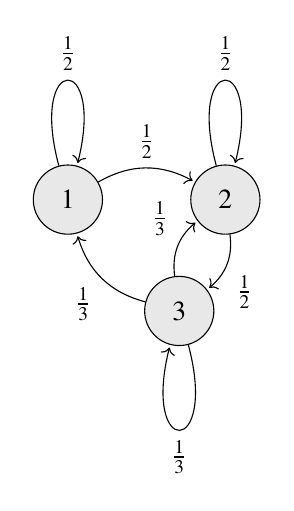
\begin{tikzpicture}[shorten >=1pt,node distance=2cm, scale =3, auto]
			\tikzstyle{every state}=[fill={rgb:black,1;white,10}]
			
			\node[state]   (q_1)                          {$1$};
			\node[state]   (q_2)  [right of=q_1]          {$2$};
			\node[state]   (q_3)  [below right of=q_1]          {$3$};
			
			\path[->]
			(q_1) edge [loop above] node {$\frac{1}{2}$}    (   )
			edge [bend left]  node {$\frac{1}{2}$}    (q_2)
			(q_2) edge [bend left]  node {$\frac{1}{2}$}    (q_3)
			edge [loop above] node {$\frac{1}{2}$}    ()
			(q_3) edge [bend left]  node {$\frac{1}{3}$}    (q_2)
			edge [bend left]  node {$\frac{1}{3}$}    (q_1)
			edge [loop below] node {$\frac{1}{3}$}    ();
		\end{tikzpicture}$
		
		\\  
		&\\
		&\\
		\hline
		\multirow{3}{*}{Checking whether the  } & \\
		& Here,\\chain is Irreducible
		& All the states are accessible to one another. \\and Aperiodic
		& $\implies$ They are in the same communication class. So, it is Irreducible.\\
		& \\
		& There exists the non- zero self-transition, which means that the chain \\
		& is Aperiodic.\\
		&\\ 
		& We know that if the Markov Chain is irreducible and aperiodic then \\
		& \qquad \qquad \qquad $\Vec{\pi}_{j} = \lim_{n \to \infty}P\{X_{n} = j\}$, $j = 1,...,N$ \\
		& These are the stationary probabilities. \\
		&\\
		\hline
		\multirow{3}{*}{Finding the Stationary} & \\
		& Stationary Probability can be represented as\\Probability Distributions
		& \qquad \qquad \qquad $\Vec{\pi} = \Vec{\pi} \vec{P}$\\
		& \\
		& \qquad $\implies$ $\myvec{v_{1}&&v_{2}&&v_{3}} = \myvec{v_{1}&&v_{2}&&v_{3}}\vec{P}$ \\
		& \\
		& Equating the above equation we get \\
		& \\
		& \qquad \qquad \qquad $\frac{1}{2}v_{1}-\frac{1}{3}v_{3} = 0$ $\label{eq:solutions/2018/dec/106/eq}$\\
		& \\
		& \qquad \qquad \qquad $\frac{1}{2}v_{1}-\frac{1}{2}v_{2} + \frac{1}{3}v_{3} = 0$\\
		& \\
		& \qquad \qquad \qquad $\frac{1}{2}v_{2}-\frac{2}{3}v_{3} = 0$\\
		& \\\
		& We see that summation of second and the third equation gives us the \\
		& first equation only. \\
		& And we know that the probability distribution will sum up to 1. \\
		& \\
		& \qquad \qquad \qquad $v_{1}+v_{2}+v_{3} = 1$ \\
		& \\
		& Therefore, we get the equation form as \\
		& \\
		& \qquad \qquad \qquad $\myvec{1&1&1\\\frac{1}{2}&0&\frac{-1}{3}\\\frac{1}{2}&\frac{-1}{2}&\frac{1}{3}}\myvec{v_{1}\\v_{2}\\v_{3}} = \myvec{1\\0\\0}$ \\
		& \\
		\hline
		\multirow{3}{*}{Solving the linear} & \\
		& The above linear equation can be solved using Gauss-Jordan method as\\equtions
		& \\
		& \qquad \qquad \qquad $\myvec{1&1&1&\vrule&1\\\frac{1}{2}&0&\frac{-1}{3}&\vrule&0\\\frac{1}{2}&\frac{-1}{2}&\frac{1}{3}&\vrule&0}$\\
		& \\
		& \qquad $\xleftrightarrow[]{R_2 \leftarrow R_2 - \frac{1}{2}R_1}$
		$\myvec{1&1&1&\vrule&1\\0&\frac{-1}{2}&\frac{-5}{6}&\vrule&\frac{-1}{2}\\\frac{1}{2}&\frac{-1}{2}&\frac{1}{3}&\vrule&0}$\\
		&\\
		& \qquad $\xleftrightarrow[]{R_3 \leftarrow R_3 - \frac{1}{2}R_1}$
		$\myvec{1&1&1&\vrule&1\\0&\frac{-1}{2}&\frac{-5}{6}&\vrule&\frac{-1}{2}\\0&-1&\frac{-1}{6}&\vrule&\frac{-1}{2}}$\\
		&\\
		& \qquad $\xleftrightarrow[]{R_2 \leftarrow \frac{-1}{2}R_2}$
		$\myvec{1&1&1&\vrule&1\\0&1&\frac{5}{3}&\vrule&1\\0&-1&\frac{-1}{6}&\vrule&\frac{-1}{2}}$\\
		&\\
		& \qquad $\xleftrightarrow[]{R_3 \leftarrow R_3 + R_2}$
		$\myvec{1&1&1&\vrule&1\\0&1&\frac{5}{3}&\vrule&1\\0&0&\frac{3}{2}&\vrule&\frac{1}{2}}$\\
		&\\
		& \qquad $\xleftrightarrow[]{R_3 \leftarrow \frac{3}{2}R_3}$
		$\myvec{1&1&1&\vrule&1\\0&1&\frac{5}{3}&\vrule&1\\0&0&1&\vrule&\frac{1}{3}}$\\
		&\\
		& \qquad $\xleftrightarrow[]{R_2 \leftarrow R_2 - \frac{5}{3}R_3}$
		$\myvec{1&1&1&\vrule&1\\0&1&0&\vrule&\frac{4}{9}\\0&0&1&\vrule&\frac{1}{3}}$\\
		&\\
		& \qquad $\xleftrightarrow[]{R_1 \leftarrow R_1 - R_3}$
		$\myvec{1&1&0&\vrule&\frac{2}{3}\\0&1&0&\vrule&\frac{4}{9}\\0&0&1&\vrule&\frac{1}{3}}$\\
		&\\
		& \qquad $\xleftrightarrow[]{R_1 \leftarrow R_1 - R_2}$
		$\myvec{1&0&0&\vrule&\frac{2}{9}\\0&1&0&\vrule&\frac{4}{9}\\0&0&1&\vrule&\frac{1}{3}}$\\
		&\\
		& $\therefore$, stationary probability distribution $\pi$ is given by \\
		& \qquad \qquad $\pi = \myvec{\frac{2}{9} & \frac{4}{9} & \frac{1}{3}}$ \\
		& \\
		\hline
		\multirow{3}{*}{Observations} & \\
		
		
		& Since the given transition probability matrix $\vec{P}$ is irreducible and aperiodic, \\
		& then $\lim_{n \to \infty} \vec{P}^{n}$ converges to a matrix with all rows identical and equal to $\vec{\pi}$. \\
		& \\
		& We were able to find $\vec{\pi}$ as $\myvec{\frac{2}{9} & \frac{4}{9} & \frac{1}{3}}$ \\
		& \\
		& $\lim_{n \to \infty} \vec{P}^{n} = \myvec{\frac{2}{9}&\frac{4}{9}&\frac{1}{3}\\\frac{2}{9}&\frac{4}{9}&\frac{1}{3}\\\frac{2}{9}&\frac{4}{9}&\frac{1}{3}}$\\
		& \\
		& From the above matrix, we get \\
		& \\
		& $\lim_{n \to \infty} \vec{P}^{n}_{11} = \frac{2}{9}$ \\
		&\\
		& $\lim_{n \to \infty} \vec{P}^{n}_{21} = \frac{2}{9}$ \\
		&\\
		& $\lim_{n \to \infty} \vec{P}^{n}_{32} = \frac{4}{9}$ \\
		&\\
		& $\lim_{n \to \infty} \vec{P}^{n}_{13} = \frac{1}{3}$ \\
		&\\
		\hline
		\multirow{3}{*}{Conclusion} & \\
		& From our observation we see that \\
		&\\
		& Options 1) and 4) are True.\\
		& \\
		\hline
\caption{}
\label{eq:solutions/2018/dec/106/table1}
	\end{longtable}
\twocolumn

%
\item Let
\begin{align}
T: \mathbb{R}^n \to \mathbb{R}^n
\end{align}
%
be a linear map that satisfies 
\begin{align}
T^2 = T-I.
\end{align}
Then which of the following is true?
\begin{enumerate}
\item $T$ is invertible. 
\item $T-I$ is not invertible. 
\item $T$ has a real eigenvalue. 
\item $T^3 = -I$ . 
\end{enumerate}
%
\solution
See Tables \ref{eq:solutions/2018/dec/106/table0} and \ref{eq:solutions/2018/dec/106/table1}


\onecolumn
	\begin{longtable}{|l|l|}
		\hline
		\multirow{3}{*}{Irreducible Markov Chain} 
		& \\
		& A Markov chain is $\textbf{irreducible}$ if all the states communicate with each other,\\
		& i.e., if there is only one communication class.\\
		&\\
		\hline
		\multirow{3}{*}{Aperiodic Markov Chain} & \\
		& If there is a self-transition in the chain ($p^{ii}>0$ for some i), then the chain is\\
		& called as $\textbf{aperiodic}$\\
		& \\
		\hline
		\multirow{3}{*}{Stationary Distribution} & \\
		& A stationary distribution of a Markov chain is a probability distribution that\\
		& remains unchanged in the Markov chain as time progresses. Typically, it is\\
		& represented as a row vector $\Vec{\pi}$ whose entries are probabilities summing to 1,\\ 
		& and given transition matrix $\textbf{P}$, it satisfies\\
		& \\
		&  \qquad \qquad  \qquad$\Vec{\pi} = \Vec{\pi} \textbf{P}$\\
		& \\
		\hline
\caption{}
\label{eq:solutions/2018/dec/106/table0}
	\end{longtable}
	\begin{longtable}{|l|l|}
		\hline
		\multirow{3}{*}{Drawing Transition diagram} 
		& \\
		& 
		
		$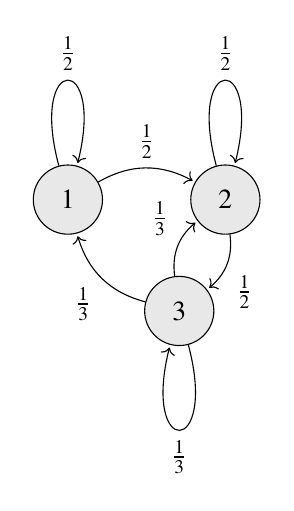
\begin{tikzpicture}[shorten >=1pt,node distance=2cm, scale =3, auto]
			\tikzstyle{every state}=[fill={rgb:black,1;white,10}]
			
			\node[state]   (q_1)                          {$1$};
			\node[state]   (q_2)  [right of=q_1]          {$2$};
			\node[state]   (q_3)  [below right of=q_1]          {$3$};
			
			\path[->]
			(q_1) edge [loop above] node {$\frac{1}{2}$}    (   )
			edge [bend left]  node {$\frac{1}{2}$}    (q_2)
			(q_2) edge [bend left]  node {$\frac{1}{2}$}    (q_3)
			edge [loop above] node {$\frac{1}{2}$}    ()
			(q_3) edge [bend left]  node {$\frac{1}{3}$}    (q_2)
			edge [bend left]  node {$\frac{1}{3}$}    (q_1)
			edge [loop below] node {$\frac{1}{3}$}    ();
		\end{tikzpicture}$
		
		\\  
		&\\
		&\\
		\hline
		\multirow{3}{*}{Checking whether the  } & \\
		& Here,\\chain is Irreducible
		& All the states are accessible to one another. \\and Aperiodic
		& $\implies$ They are in the same communication class. So, it is Irreducible.\\
		& \\
		& There exists the non- zero self-transition, which means that the chain \\
		& is Aperiodic.\\
		&\\ 
		& We know that if the Markov Chain is irreducible and aperiodic then \\
		& \qquad \qquad \qquad $\Vec{\pi}_{j} = \lim_{n \to \infty}P\{X_{n} = j\}$, $j = 1,...,N$ \\
		& These are the stationary probabilities. \\
		&\\
		\hline
		\multirow{3}{*}{Finding the Stationary} & \\
		& Stationary Probability can be represented as\\Probability Distributions
		& \qquad \qquad \qquad $\Vec{\pi} = \Vec{\pi} \vec{P}$\\
		& \\
		& \qquad $\implies$ $\myvec{v_{1}&&v_{2}&&v_{3}} = \myvec{v_{1}&&v_{2}&&v_{3}}\vec{P}$ \\
		& \\
		& Equating the above equation we get \\
		& \\
		& \qquad \qquad \qquad $\frac{1}{2}v_{1}-\frac{1}{3}v_{3} = 0$ $\label{eq:solutions/2018/dec/106/eq}$\\
		& \\
		& \qquad \qquad \qquad $\frac{1}{2}v_{1}-\frac{1}{2}v_{2} + \frac{1}{3}v_{3} = 0$\\
		& \\
		& \qquad \qquad \qquad $\frac{1}{2}v_{2}-\frac{2}{3}v_{3} = 0$\\
		& \\\
		& We see that summation of second and the third equation gives us the \\
		& first equation only. \\
		& And we know that the probability distribution will sum up to 1. \\
		& \\
		& \qquad \qquad \qquad $v_{1}+v_{2}+v_{3} = 1$ \\
		& \\
		& Therefore, we get the equation form as \\
		& \\
		& \qquad \qquad \qquad $\myvec{1&1&1\\\frac{1}{2}&0&\frac{-1}{3}\\\frac{1}{2}&\frac{-1}{2}&\frac{1}{3}}\myvec{v_{1}\\v_{2}\\v_{3}} = \myvec{1\\0\\0}$ \\
		& \\
		\hline
		\multirow{3}{*}{Solving the linear} & \\
		& The above linear equation can be solved using Gauss-Jordan method as\\equtions
		& \\
		& \qquad \qquad \qquad $\myvec{1&1&1&\vrule&1\\\frac{1}{2}&0&\frac{-1}{3}&\vrule&0\\\frac{1}{2}&\frac{-1}{2}&\frac{1}{3}&\vrule&0}$\\
		& \\
		& \qquad $\xleftrightarrow[]{R_2 \leftarrow R_2 - \frac{1}{2}R_1}$
		$\myvec{1&1&1&\vrule&1\\0&\frac{-1}{2}&\frac{-5}{6}&\vrule&\frac{-1}{2}\\\frac{1}{2}&\frac{-1}{2}&\frac{1}{3}&\vrule&0}$\\
		&\\
		& \qquad $\xleftrightarrow[]{R_3 \leftarrow R_3 - \frac{1}{2}R_1}$
		$\myvec{1&1&1&\vrule&1\\0&\frac{-1}{2}&\frac{-5}{6}&\vrule&\frac{-1}{2}\\0&-1&\frac{-1}{6}&\vrule&\frac{-1}{2}}$\\
		&\\
		& \qquad $\xleftrightarrow[]{R_2 \leftarrow \frac{-1}{2}R_2}$
		$\myvec{1&1&1&\vrule&1\\0&1&\frac{5}{3}&\vrule&1\\0&-1&\frac{-1}{6}&\vrule&\frac{-1}{2}}$\\
		&\\
		& \qquad $\xleftrightarrow[]{R_3 \leftarrow R_3 + R_2}$
		$\myvec{1&1&1&\vrule&1\\0&1&\frac{5}{3}&\vrule&1\\0&0&\frac{3}{2}&\vrule&\frac{1}{2}}$\\
		&\\
		& \qquad $\xleftrightarrow[]{R_3 \leftarrow \frac{3}{2}R_3}$
		$\myvec{1&1&1&\vrule&1\\0&1&\frac{5}{3}&\vrule&1\\0&0&1&\vrule&\frac{1}{3}}$\\
		&\\
		& \qquad $\xleftrightarrow[]{R_2 \leftarrow R_2 - \frac{5}{3}R_3}$
		$\myvec{1&1&1&\vrule&1\\0&1&0&\vrule&\frac{4}{9}\\0&0&1&\vrule&\frac{1}{3}}$\\
		&\\
		& \qquad $\xleftrightarrow[]{R_1 \leftarrow R_1 - R_3}$
		$\myvec{1&1&0&\vrule&\frac{2}{3}\\0&1&0&\vrule&\frac{4}{9}\\0&0&1&\vrule&\frac{1}{3}}$\\
		&\\
		& \qquad $\xleftrightarrow[]{R_1 \leftarrow R_1 - R_2}$
		$\myvec{1&0&0&\vrule&\frac{2}{9}\\0&1&0&\vrule&\frac{4}{9}\\0&0&1&\vrule&\frac{1}{3}}$\\
		&\\
		& $\therefore$, stationary probability distribution $\pi$ is given by \\
		& \qquad \qquad $\pi = \myvec{\frac{2}{9} & \frac{4}{9} & \frac{1}{3}}$ \\
		& \\
		\hline
		\multirow{3}{*}{Observations} & \\
		
		
		& Since the given transition probability matrix $\vec{P}$ is irreducible and aperiodic, \\
		& then $\lim_{n \to \infty} \vec{P}^{n}$ converges to a matrix with all rows identical and equal to $\vec{\pi}$. \\
		& \\
		& We were able to find $\vec{\pi}$ as $\myvec{\frac{2}{9} & \frac{4}{9} & \frac{1}{3}}$ \\
		& \\
		& $\lim_{n \to \infty} \vec{P}^{n} = \myvec{\frac{2}{9}&\frac{4}{9}&\frac{1}{3}\\\frac{2}{9}&\frac{4}{9}&\frac{1}{3}\\\frac{2}{9}&\frac{4}{9}&\frac{1}{3}}$\\
		& \\
		& From the above matrix, we get \\
		& \\
		& $\lim_{n \to \infty} \vec{P}^{n}_{11} = \frac{2}{9}$ \\
		&\\
		& $\lim_{n \to \infty} \vec{P}^{n}_{21} = \frac{2}{9}$ \\
		&\\
		& $\lim_{n \to \infty} \vec{P}^{n}_{32} = \frac{4}{9}$ \\
		&\\
		& $\lim_{n \to \infty} \vec{P}^{n}_{13} = \frac{1}{3}$ \\
		&\\
		\hline
		\multirow{3}{*}{Conclusion} & \\
		& From our observation we see that \\
		&\\
		& Options 1) and 4) are True.\\
		& \\
		\hline
\caption{}
\label{eq:solutions/2018/dec/106/table1}
	\end{longtable}
\twocolumn

\item Let
\begin{align}
\vec{M} = 
\myvec
{
2 & 0 & 3 & 2 & 0 & -2
\\
0 & 1 & 0 & -1 & 3 & 4
\\
0 & 0 & 1 & 0 & 4 & 4
\\
1 & 1 & 1 & 0 & 1 & 1
}
\\
\vec{b}_1 = \myvec{5 \\ 1 \\ 1 \\ 4},
\vec{b}_2 = \myvec{5 \\ 1 \\ 3 \\ 3}.
\end{align}  
Then which of the following are true?
\begin{enumerate}
\item both systems $\vec{M}\vec{x} = \vec{b}_1$ and $\vec{M}\vec{x} = \vec{b}_2$ are inconsistent.
\item both systems $\vec{M}\vec{x} = \vec{b}_1$ and $\vec{M}\vec{x} = \vec{b}_2$ are consistent. 
\item the system $\vec{M}\vec{x} = \vec{b}_1-\vec{b}_2$ is consistent. 
\item the system $\vec{M}\vec{x} = \vec{b}_1-\vec{b}_2$ is inconsistent. 
\end{enumerate}
%
%
\solution
See Tables \ref{eq:solutions/2018/dec/106/table0} and \ref{eq:solutions/2018/dec/106/table1}


\onecolumn
	\begin{longtable}{|l|l|}
		\hline
		\multirow{3}{*}{Irreducible Markov Chain} 
		& \\
		& A Markov chain is $\textbf{irreducible}$ if all the states communicate with each other,\\
		& i.e., if there is only one communication class.\\
		&\\
		\hline
		\multirow{3}{*}{Aperiodic Markov Chain} & \\
		& If there is a self-transition in the chain ($p^{ii}>0$ for some i), then the chain is\\
		& called as $\textbf{aperiodic}$\\
		& \\
		\hline
		\multirow{3}{*}{Stationary Distribution} & \\
		& A stationary distribution of a Markov chain is a probability distribution that\\
		& remains unchanged in the Markov chain as time progresses. Typically, it is\\
		& represented as a row vector $\Vec{\pi}$ whose entries are probabilities summing to 1,\\ 
		& and given transition matrix $\textbf{P}$, it satisfies\\
		& \\
		&  \qquad \qquad  \qquad$\Vec{\pi} = \Vec{\pi} \textbf{P}$\\
		& \\
		\hline
\caption{}
\label{eq:solutions/2018/dec/106/table0}
	\end{longtable}
	\begin{longtable}{|l|l|}
		\hline
		\multirow{3}{*}{Drawing Transition diagram} 
		& \\
		& 
		
		$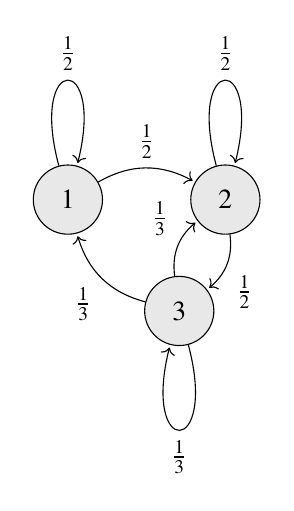
\begin{tikzpicture}[shorten >=1pt,node distance=2cm, scale =3, auto]
			\tikzstyle{every state}=[fill={rgb:black,1;white,10}]
			
			\node[state]   (q_1)                          {$1$};
			\node[state]   (q_2)  [right of=q_1]          {$2$};
			\node[state]   (q_3)  [below right of=q_1]          {$3$};
			
			\path[->]
			(q_1) edge [loop above] node {$\frac{1}{2}$}    (   )
			edge [bend left]  node {$\frac{1}{2}$}    (q_2)
			(q_2) edge [bend left]  node {$\frac{1}{2}$}    (q_3)
			edge [loop above] node {$\frac{1}{2}$}    ()
			(q_3) edge [bend left]  node {$\frac{1}{3}$}    (q_2)
			edge [bend left]  node {$\frac{1}{3}$}    (q_1)
			edge [loop below] node {$\frac{1}{3}$}    ();
		\end{tikzpicture}$
		
		\\  
		&\\
		&\\
		\hline
		\multirow{3}{*}{Checking whether the  } & \\
		& Here,\\chain is Irreducible
		& All the states are accessible to one another. \\and Aperiodic
		& $\implies$ They are in the same communication class. So, it is Irreducible.\\
		& \\
		& There exists the non- zero self-transition, which means that the chain \\
		& is Aperiodic.\\
		&\\ 
		& We know that if the Markov Chain is irreducible and aperiodic then \\
		& \qquad \qquad \qquad $\Vec{\pi}_{j} = \lim_{n \to \infty}P\{X_{n} = j\}$, $j = 1,...,N$ \\
		& These are the stationary probabilities. \\
		&\\
		\hline
		\multirow{3}{*}{Finding the Stationary} & \\
		& Stationary Probability can be represented as\\Probability Distributions
		& \qquad \qquad \qquad $\Vec{\pi} = \Vec{\pi} \vec{P}$\\
		& \\
		& \qquad $\implies$ $\myvec{v_{1}&&v_{2}&&v_{3}} = \myvec{v_{1}&&v_{2}&&v_{3}}\vec{P}$ \\
		& \\
		& Equating the above equation we get \\
		& \\
		& \qquad \qquad \qquad $\frac{1}{2}v_{1}-\frac{1}{3}v_{3} = 0$ $\label{eq:solutions/2018/dec/106/eq}$\\
		& \\
		& \qquad \qquad \qquad $\frac{1}{2}v_{1}-\frac{1}{2}v_{2} + \frac{1}{3}v_{3} = 0$\\
		& \\
		& \qquad \qquad \qquad $\frac{1}{2}v_{2}-\frac{2}{3}v_{3} = 0$\\
		& \\\
		& We see that summation of second and the third equation gives us the \\
		& first equation only. \\
		& And we know that the probability distribution will sum up to 1. \\
		& \\
		& \qquad \qquad \qquad $v_{1}+v_{2}+v_{3} = 1$ \\
		& \\
		& Therefore, we get the equation form as \\
		& \\
		& \qquad \qquad \qquad $\myvec{1&1&1\\\frac{1}{2}&0&\frac{-1}{3}\\\frac{1}{2}&\frac{-1}{2}&\frac{1}{3}}\myvec{v_{1}\\v_{2}\\v_{3}} = \myvec{1\\0\\0}$ \\
		& \\
		\hline
		\multirow{3}{*}{Solving the linear} & \\
		& The above linear equation can be solved using Gauss-Jordan method as\\equtions
		& \\
		& \qquad \qquad \qquad $\myvec{1&1&1&\vrule&1\\\frac{1}{2}&0&\frac{-1}{3}&\vrule&0\\\frac{1}{2}&\frac{-1}{2}&\frac{1}{3}&\vrule&0}$\\
		& \\
		& \qquad $\xleftrightarrow[]{R_2 \leftarrow R_2 - \frac{1}{2}R_1}$
		$\myvec{1&1&1&\vrule&1\\0&\frac{-1}{2}&\frac{-5}{6}&\vrule&\frac{-1}{2}\\\frac{1}{2}&\frac{-1}{2}&\frac{1}{3}&\vrule&0}$\\
		&\\
		& \qquad $\xleftrightarrow[]{R_3 \leftarrow R_3 - \frac{1}{2}R_1}$
		$\myvec{1&1&1&\vrule&1\\0&\frac{-1}{2}&\frac{-5}{6}&\vrule&\frac{-1}{2}\\0&-1&\frac{-1}{6}&\vrule&\frac{-1}{2}}$\\
		&\\
		& \qquad $\xleftrightarrow[]{R_2 \leftarrow \frac{-1}{2}R_2}$
		$\myvec{1&1&1&\vrule&1\\0&1&\frac{5}{3}&\vrule&1\\0&-1&\frac{-1}{6}&\vrule&\frac{-1}{2}}$\\
		&\\
		& \qquad $\xleftrightarrow[]{R_3 \leftarrow R_3 + R_2}$
		$\myvec{1&1&1&\vrule&1\\0&1&\frac{5}{3}&\vrule&1\\0&0&\frac{3}{2}&\vrule&\frac{1}{2}}$\\
		&\\
		& \qquad $\xleftrightarrow[]{R_3 \leftarrow \frac{3}{2}R_3}$
		$\myvec{1&1&1&\vrule&1\\0&1&\frac{5}{3}&\vrule&1\\0&0&1&\vrule&\frac{1}{3}}$\\
		&\\
		& \qquad $\xleftrightarrow[]{R_2 \leftarrow R_2 - \frac{5}{3}R_3}$
		$\myvec{1&1&1&\vrule&1\\0&1&0&\vrule&\frac{4}{9}\\0&0&1&\vrule&\frac{1}{3}}$\\
		&\\
		& \qquad $\xleftrightarrow[]{R_1 \leftarrow R_1 - R_3}$
		$\myvec{1&1&0&\vrule&\frac{2}{3}\\0&1&0&\vrule&\frac{4}{9}\\0&0&1&\vrule&\frac{1}{3}}$\\
		&\\
		& \qquad $\xleftrightarrow[]{R_1 \leftarrow R_1 - R_2}$
		$\myvec{1&0&0&\vrule&\frac{2}{9}\\0&1&0&\vrule&\frac{4}{9}\\0&0&1&\vrule&\frac{1}{3}}$\\
		&\\
		& $\therefore$, stationary probability distribution $\pi$ is given by \\
		& \qquad \qquad $\pi = \myvec{\frac{2}{9} & \frac{4}{9} & \frac{1}{3}}$ \\
		& \\
		\hline
		\multirow{3}{*}{Observations} & \\
		
		
		& Since the given transition probability matrix $\vec{P}$ is irreducible and aperiodic, \\
		& then $\lim_{n \to \infty} \vec{P}^{n}$ converges to a matrix with all rows identical and equal to $\vec{\pi}$. \\
		& \\
		& We were able to find $\vec{\pi}$ as $\myvec{\frac{2}{9} & \frac{4}{9} & \frac{1}{3}}$ \\
		& \\
		& $\lim_{n \to \infty} \vec{P}^{n} = \myvec{\frac{2}{9}&\frac{4}{9}&\frac{1}{3}\\\frac{2}{9}&\frac{4}{9}&\frac{1}{3}\\\frac{2}{9}&\frac{4}{9}&\frac{1}{3}}$\\
		& \\
		& From the above matrix, we get \\
		& \\
		& $\lim_{n \to \infty} \vec{P}^{n}_{11} = \frac{2}{9}$ \\
		&\\
		& $\lim_{n \to \infty} \vec{P}^{n}_{21} = \frac{2}{9}$ \\
		&\\
		& $\lim_{n \to \infty} \vec{P}^{n}_{32} = \frac{4}{9}$ \\
		&\\
		& $\lim_{n \to \infty} \vec{P}^{n}_{13} = \frac{1}{3}$ \\
		&\\
		\hline
		\multirow{3}{*}{Conclusion} & \\
		& From our observation we see that \\
		&\\
		& Options 1) and 4) are True.\\
		& \\
		\hline
\caption{}
\label{eq:solutions/2018/dec/106/table1}
	\end{longtable}
\twocolumn

\item Let 
\begin{align}
\vec{M} = \myvec
{
1 & -1 & 1 \\
2 & 1 & 4 \\
-2 & 1 & -4 
}.
\end{align}
Given that 1 is an eigenvalue of $\vec{M}$, then which among the following
are correct?
\begin{enumerate}
\item The minimal polynomial of  $\vec{M}$ is $\brak{x-1}\brak{x+4}$ 
\item The minimal polynomial of  $\vec{M}$ is $\brak{x-1}^2\brak{x+4}$ 
\item   $\vec{M}$ is not diagonalizable.
\item $\vec{M}^{-1} = \frac{1}{4}\brak{\vec{M}+3\vec{I}}$. 
\end{enumerate}
%
\solution
See Tables \ref{eq:solutions/2018/dec/106/table0} and \ref{eq:solutions/2018/dec/106/table1}


\onecolumn
	\begin{longtable}{|l|l|}
		\hline
		\multirow{3}{*}{Irreducible Markov Chain} 
		& \\
		& A Markov chain is $\textbf{irreducible}$ if all the states communicate with each other,\\
		& i.e., if there is only one communication class.\\
		&\\
		\hline
		\multirow{3}{*}{Aperiodic Markov Chain} & \\
		& If there is a self-transition in the chain ($p^{ii}>0$ for some i), then the chain is\\
		& called as $\textbf{aperiodic}$\\
		& \\
		\hline
		\multirow{3}{*}{Stationary Distribution} & \\
		& A stationary distribution of a Markov chain is a probability distribution that\\
		& remains unchanged in the Markov chain as time progresses. Typically, it is\\
		& represented as a row vector $\Vec{\pi}$ whose entries are probabilities summing to 1,\\ 
		& and given transition matrix $\textbf{P}$, it satisfies\\
		& \\
		&  \qquad \qquad  \qquad$\Vec{\pi} = \Vec{\pi} \textbf{P}$\\
		& \\
		\hline
\caption{}
\label{eq:solutions/2018/dec/106/table0}
	\end{longtable}
	\begin{longtable}{|l|l|}
		\hline
		\multirow{3}{*}{Drawing Transition diagram} 
		& \\
		& 
		
		$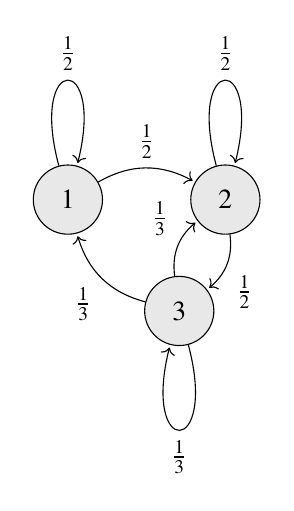
\begin{tikzpicture}[shorten >=1pt,node distance=2cm, scale =3, auto]
			\tikzstyle{every state}=[fill={rgb:black,1;white,10}]
			
			\node[state]   (q_1)                          {$1$};
			\node[state]   (q_2)  [right of=q_1]          {$2$};
			\node[state]   (q_3)  [below right of=q_1]          {$3$};
			
			\path[->]
			(q_1) edge [loop above] node {$\frac{1}{2}$}    (   )
			edge [bend left]  node {$\frac{1}{2}$}    (q_2)
			(q_2) edge [bend left]  node {$\frac{1}{2}$}    (q_3)
			edge [loop above] node {$\frac{1}{2}$}    ()
			(q_3) edge [bend left]  node {$\frac{1}{3}$}    (q_2)
			edge [bend left]  node {$\frac{1}{3}$}    (q_1)
			edge [loop below] node {$\frac{1}{3}$}    ();
		\end{tikzpicture}$
		
		\\  
		&\\
		&\\
		\hline
		\multirow{3}{*}{Checking whether the  } & \\
		& Here,\\chain is Irreducible
		& All the states are accessible to one another. \\and Aperiodic
		& $\implies$ They are in the same communication class. So, it is Irreducible.\\
		& \\
		& There exists the non- zero self-transition, which means that the chain \\
		& is Aperiodic.\\
		&\\ 
		& We know that if the Markov Chain is irreducible and aperiodic then \\
		& \qquad \qquad \qquad $\Vec{\pi}_{j} = \lim_{n \to \infty}P\{X_{n} = j\}$, $j = 1,...,N$ \\
		& These are the stationary probabilities. \\
		&\\
		\hline
		\multirow{3}{*}{Finding the Stationary} & \\
		& Stationary Probability can be represented as\\Probability Distributions
		& \qquad \qquad \qquad $\Vec{\pi} = \Vec{\pi} \vec{P}$\\
		& \\
		& \qquad $\implies$ $\myvec{v_{1}&&v_{2}&&v_{3}} = \myvec{v_{1}&&v_{2}&&v_{3}}\vec{P}$ \\
		& \\
		& Equating the above equation we get \\
		& \\
		& \qquad \qquad \qquad $\frac{1}{2}v_{1}-\frac{1}{3}v_{3} = 0$ $\label{eq:solutions/2018/dec/106/eq}$\\
		& \\
		& \qquad \qquad \qquad $\frac{1}{2}v_{1}-\frac{1}{2}v_{2} + \frac{1}{3}v_{3} = 0$\\
		& \\
		& \qquad \qquad \qquad $\frac{1}{2}v_{2}-\frac{2}{3}v_{3} = 0$\\
		& \\\
		& We see that summation of second and the third equation gives us the \\
		& first equation only. \\
		& And we know that the probability distribution will sum up to 1. \\
		& \\
		& \qquad \qquad \qquad $v_{1}+v_{2}+v_{3} = 1$ \\
		& \\
		& Therefore, we get the equation form as \\
		& \\
		& \qquad \qquad \qquad $\myvec{1&1&1\\\frac{1}{2}&0&\frac{-1}{3}\\\frac{1}{2}&\frac{-1}{2}&\frac{1}{3}}\myvec{v_{1}\\v_{2}\\v_{3}} = \myvec{1\\0\\0}$ \\
		& \\
		\hline
		\multirow{3}{*}{Solving the linear} & \\
		& The above linear equation can be solved using Gauss-Jordan method as\\equtions
		& \\
		& \qquad \qquad \qquad $\myvec{1&1&1&\vrule&1\\\frac{1}{2}&0&\frac{-1}{3}&\vrule&0\\\frac{1}{2}&\frac{-1}{2}&\frac{1}{3}&\vrule&0}$\\
		& \\
		& \qquad $\xleftrightarrow[]{R_2 \leftarrow R_2 - \frac{1}{2}R_1}$
		$\myvec{1&1&1&\vrule&1\\0&\frac{-1}{2}&\frac{-5}{6}&\vrule&\frac{-1}{2}\\\frac{1}{2}&\frac{-1}{2}&\frac{1}{3}&\vrule&0}$\\
		&\\
		& \qquad $\xleftrightarrow[]{R_3 \leftarrow R_3 - \frac{1}{2}R_1}$
		$\myvec{1&1&1&\vrule&1\\0&\frac{-1}{2}&\frac{-5}{6}&\vrule&\frac{-1}{2}\\0&-1&\frac{-1}{6}&\vrule&\frac{-1}{2}}$\\
		&\\
		& \qquad $\xleftrightarrow[]{R_2 \leftarrow \frac{-1}{2}R_2}$
		$\myvec{1&1&1&\vrule&1\\0&1&\frac{5}{3}&\vrule&1\\0&-1&\frac{-1}{6}&\vrule&\frac{-1}{2}}$\\
		&\\
		& \qquad $\xleftrightarrow[]{R_3 \leftarrow R_3 + R_2}$
		$\myvec{1&1&1&\vrule&1\\0&1&\frac{5}{3}&\vrule&1\\0&0&\frac{3}{2}&\vrule&\frac{1}{2}}$\\
		&\\
		& \qquad $\xleftrightarrow[]{R_3 \leftarrow \frac{3}{2}R_3}$
		$\myvec{1&1&1&\vrule&1\\0&1&\frac{5}{3}&\vrule&1\\0&0&1&\vrule&\frac{1}{3}}$\\
		&\\
		& \qquad $\xleftrightarrow[]{R_2 \leftarrow R_2 - \frac{5}{3}R_3}$
		$\myvec{1&1&1&\vrule&1\\0&1&0&\vrule&\frac{4}{9}\\0&0&1&\vrule&\frac{1}{3}}$\\
		&\\
		& \qquad $\xleftrightarrow[]{R_1 \leftarrow R_1 - R_3}$
		$\myvec{1&1&0&\vrule&\frac{2}{3}\\0&1&0&\vrule&\frac{4}{9}\\0&0&1&\vrule&\frac{1}{3}}$\\
		&\\
		& \qquad $\xleftrightarrow[]{R_1 \leftarrow R_1 - R_2}$
		$\myvec{1&0&0&\vrule&\frac{2}{9}\\0&1&0&\vrule&\frac{4}{9}\\0&0&1&\vrule&\frac{1}{3}}$\\
		&\\
		& $\therefore$, stationary probability distribution $\pi$ is given by \\
		& \qquad \qquad $\pi = \myvec{\frac{2}{9} & \frac{4}{9} & \frac{1}{3}}$ \\
		& \\
		\hline
		\multirow{3}{*}{Observations} & \\
		
		
		& Since the given transition probability matrix $\vec{P}$ is irreducible and aperiodic, \\
		& then $\lim_{n \to \infty} \vec{P}^{n}$ converges to a matrix with all rows identical and equal to $\vec{\pi}$. \\
		& \\
		& We were able to find $\vec{\pi}$ as $\myvec{\frac{2}{9} & \frac{4}{9} & \frac{1}{3}}$ \\
		& \\
		& $\lim_{n \to \infty} \vec{P}^{n} = \myvec{\frac{2}{9}&\frac{4}{9}&\frac{1}{3}\\\frac{2}{9}&\frac{4}{9}&\frac{1}{3}\\\frac{2}{9}&\frac{4}{9}&\frac{1}{3}}$\\
		& \\
		& From the above matrix, we get \\
		& \\
		& $\lim_{n \to \infty} \vec{P}^{n}_{11} = \frac{2}{9}$ \\
		&\\
		& $\lim_{n \to \infty} \vec{P}^{n}_{21} = \frac{2}{9}$ \\
		&\\
		& $\lim_{n \to \infty} \vec{P}^{n}_{32} = \frac{4}{9}$ \\
		&\\
		& $\lim_{n \to \infty} \vec{P}^{n}_{13} = \frac{1}{3}$ \\
		&\\
		\hline
		\multirow{3}{*}{Conclusion} & \\
		& From our observation we see that \\
		&\\
		& Options 1) and 4) are True.\\
		& \\
		\hline
\caption{}
\label{eq:solutions/2018/dec/106/table1}
	\end{longtable}
\twocolumn

\item Let $\vec{A}$ be a real matrix with characteristic polynomial $\brak{x-1}^3$.  Pick the correct statements from below:
\begin{enumerate}
\item $\vec{A}$ is necessarily diagonalizable.
\item If the minimal polynomial of  $\vec{A}$ is $\brak{x-1}^3$, then  $\vec{A}$ is diagonalizable.
\item  The characteristic polynomial of  $\vec{A}^2$ is $\brak{x-1}^3$
\item If $\vec{A}$ has exactly two Jordan blocks, then $\brak{\vec{A}-\vec{I}}^2$ is diagonalizable. 
\end{enumerate}
\solution
See Tables \ref{eq:solutions/2018/dec/106/table0} and \ref{eq:solutions/2018/dec/106/table1}


\onecolumn
	\begin{longtable}{|l|l|}
		\hline
		\multirow{3}{*}{Irreducible Markov Chain} 
		& \\
		& A Markov chain is $\textbf{irreducible}$ if all the states communicate with each other,\\
		& i.e., if there is only one communication class.\\
		&\\
		\hline
		\multirow{3}{*}{Aperiodic Markov Chain} & \\
		& If there is a self-transition in the chain ($p^{ii}>0$ for some i), then the chain is\\
		& called as $\textbf{aperiodic}$\\
		& \\
		\hline
		\multirow{3}{*}{Stationary Distribution} & \\
		& A stationary distribution of a Markov chain is a probability distribution that\\
		& remains unchanged in the Markov chain as time progresses. Typically, it is\\
		& represented as a row vector $\Vec{\pi}$ whose entries are probabilities summing to 1,\\ 
		& and given transition matrix $\textbf{P}$, it satisfies\\
		& \\
		&  \qquad \qquad  \qquad$\Vec{\pi} = \Vec{\pi} \textbf{P}$\\
		& \\
		\hline
\caption{}
\label{eq:solutions/2018/dec/106/table0}
	\end{longtable}
	\begin{longtable}{|l|l|}
		\hline
		\multirow{3}{*}{Drawing Transition diagram} 
		& \\
		& 
		
		$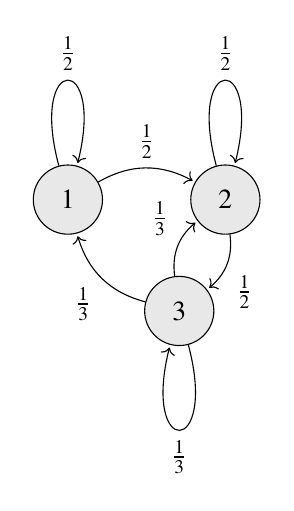
\begin{tikzpicture}[shorten >=1pt,node distance=2cm, scale =3, auto]
			\tikzstyle{every state}=[fill={rgb:black,1;white,10}]
			
			\node[state]   (q_1)                          {$1$};
			\node[state]   (q_2)  [right of=q_1]          {$2$};
			\node[state]   (q_3)  [below right of=q_1]          {$3$};
			
			\path[->]
			(q_1) edge [loop above] node {$\frac{1}{2}$}    (   )
			edge [bend left]  node {$\frac{1}{2}$}    (q_2)
			(q_2) edge [bend left]  node {$\frac{1}{2}$}    (q_3)
			edge [loop above] node {$\frac{1}{2}$}    ()
			(q_3) edge [bend left]  node {$\frac{1}{3}$}    (q_2)
			edge [bend left]  node {$\frac{1}{3}$}    (q_1)
			edge [loop below] node {$\frac{1}{3}$}    ();
		\end{tikzpicture}$
		
		\\  
		&\\
		&\\
		\hline
		\multirow{3}{*}{Checking whether the  } & \\
		& Here,\\chain is Irreducible
		& All the states are accessible to one another. \\and Aperiodic
		& $\implies$ They are in the same communication class. So, it is Irreducible.\\
		& \\
		& There exists the non- zero self-transition, which means that the chain \\
		& is Aperiodic.\\
		&\\ 
		& We know that if the Markov Chain is irreducible and aperiodic then \\
		& \qquad \qquad \qquad $\Vec{\pi}_{j} = \lim_{n \to \infty}P\{X_{n} = j\}$, $j = 1,...,N$ \\
		& These are the stationary probabilities. \\
		&\\
		\hline
		\multirow{3}{*}{Finding the Stationary} & \\
		& Stationary Probability can be represented as\\Probability Distributions
		& \qquad \qquad \qquad $\Vec{\pi} = \Vec{\pi} \vec{P}$\\
		& \\
		& \qquad $\implies$ $\myvec{v_{1}&&v_{2}&&v_{3}} = \myvec{v_{1}&&v_{2}&&v_{3}}\vec{P}$ \\
		& \\
		& Equating the above equation we get \\
		& \\
		& \qquad \qquad \qquad $\frac{1}{2}v_{1}-\frac{1}{3}v_{3} = 0$ $\label{eq:solutions/2018/dec/106/eq}$\\
		& \\
		& \qquad \qquad \qquad $\frac{1}{2}v_{1}-\frac{1}{2}v_{2} + \frac{1}{3}v_{3} = 0$\\
		& \\
		& \qquad \qquad \qquad $\frac{1}{2}v_{2}-\frac{2}{3}v_{3} = 0$\\
		& \\\
		& We see that summation of second and the third equation gives us the \\
		& first equation only. \\
		& And we know that the probability distribution will sum up to 1. \\
		& \\
		& \qquad \qquad \qquad $v_{1}+v_{2}+v_{3} = 1$ \\
		& \\
		& Therefore, we get the equation form as \\
		& \\
		& \qquad \qquad \qquad $\myvec{1&1&1\\\frac{1}{2}&0&\frac{-1}{3}\\\frac{1}{2}&\frac{-1}{2}&\frac{1}{3}}\myvec{v_{1}\\v_{2}\\v_{3}} = \myvec{1\\0\\0}$ \\
		& \\
		\hline
		\multirow{3}{*}{Solving the linear} & \\
		& The above linear equation can be solved using Gauss-Jordan method as\\equtions
		& \\
		& \qquad \qquad \qquad $\myvec{1&1&1&\vrule&1\\\frac{1}{2}&0&\frac{-1}{3}&\vrule&0\\\frac{1}{2}&\frac{-1}{2}&\frac{1}{3}&\vrule&0}$\\
		& \\
		& \qquad $\xleftrightarrow[]{R_2 \leftarrow R_2 - \frac{1}{2}R_1}$
		$\myvec{1&1&1&\vrule&1\\0&\frac{-1}{2}&\frac{-5}{6}&\vrule&\frac{-1}{2}\\\frac{1}{2}&\frac{-1}{2}&\frac{1}{3}&\vrule&0}$\\
		&\\
		& \qquad $\xleftrightarrow[]{R_3 \leftarrow R_3 - \frac{1}{2}R_1}$
		$\myvec{1&1&1&\vrule&1\\0&\frac{-1}{2}&\frac{-5}{6}&\vrule&\frac{-1}{2}\\0&-1&\frac{-1}{6}&\vrule&\frac{-1}{2}}$\\
		&\\
		& \qquad $\xleftrightarrow[]{R_2 \leftarrow \frac{-1}{2}R_2}$
		$\myvec{1&1&1&\vrule&1\\0&1&\frac{5}{3}&\vrule&1\\0&-1&\frac{-1}{6}&\vrule&\frac{-1}{2}}$\\
		&\\
		& \qquad $\xleftrightarrow[]{R_3 \leftarrow R_3 + R_2}$
		$\myvec{1&1&1&\vrule&1\\0&1&\frac{5}{3}&\vrule&1\\0&0&\frac{3}{2}&\vrule&\frac{1}{2}}$\\
		&\\
		& \qquad $\xleftrightarrow[]{R_3 \leftarrow \frac{3}{2}R_3}$
		$\myvec{1&1&1&\vrule&1\\0&1&\frac{5}{3}&\vrule&1\\0&0&1&\vrule&\frac{1}{3}}$\\
		&\\
		& \qquad $\xleftrightarrow[]{R_2 \leftarrow R_2 - \frac{5}{3}R_3}$
		$\myvec{1&1&1&\vrule&1\\0&1&0&\vrule&\frac{4}{9}\\0&0&1&\vrule&\frac{1}{3}}$\\
		&\\
		& \qquad $\xleftrightarrow[]{R_1 \leftarrow R_1 - R_3}$
		$\myvec{1&1&0&\vrule&\frac{2}{3}\\0&1&0&\vrule&\frac{4}{9}\\0&0&1&\vrule&\frac{1}{3}}$\\
		&\\
		& \qquad $\xleftrightarrow[]{R_1 \leftarrow R_1 - R_2}$
		$\myvec{1&0&0&\vrule&\frac{2}{9}\\0&1&0&\vrule&\frac{4}{9}\\0&0&1&\vrule&\frac{1}{3}}$\\
		&\\
		& $\therefore$, stationary probability distribution $\pi$ is given by \\
		& \qquad \qquad $\pi = \myvec{\frac{2}{9} & \frac{4}{9} & \frac{1}{3}}$ \\
		& \\
		\hline
		\multirow{3}{*}{Observations} & \\
		
		
		& Since the given transition probability matrix $\vec{P}$ is irreducible and aperiodic, \\
		& then $\lim_{n \to \infty} \vec{P}^{n}$ converges to a matrix with all rows identical and equal to $\vec{\pi}$. \\
		& \\
		& We were able to find $\vec{\pi}$ as $\myvec{\frac{2}{9} & \frac{4}{9} & \frac{1}{3}}$ \\
		& \\
		& $\lim_{n \to \infty} \vec{P}^{n} = \myvec{\frac{2}{9}&\frac{4}{9}&\frac{1}{3}\\\frac{2}{9}&\frac{4}{9}&\frac{1}{3}\\\frac{2}{9}&\frac{4}{9}&\frac{1}{3}}$\\
		& \\
		& From the above matrix, we get \\
		& \\
		& $\lim_{n \to \infty} \vec{P}^{n}_{11} = \frac{2}{9}$ \\
		&\\
		& $\lim_{n \to \infty} \vec{P}^{n}_{21} = \frac{2}{9}$ \\
		&\\
		& $\lim_{n \to \infty} \vec{P}^{n}_{32} = \frac{4}{9}$ \\
		&\\
		& $\lim_{n \to \infty} \vec{P}^{n}_{13} = \frac{1}{3}$ \\
		&\\
		\hline
		\multirow{3}{*}{Conclusion} & \\
		& From our observation we see that \\
		&\\
		& Options 1) and 4) are True.\\
		& \\
		\hline
\caption{}
\label{eq:solutions/2018/dec/106/table1}
	\end{longtable}
\twocolumn

%
\item Let $P_3$ be the vector space of polynomails with real coefficients and of degree at most 3.  Consider the linear map
\begin{align}
T:P_3\to P_3
\end{align}
defined by 
\begin{align}
T\brak{p(x)} = p(x-1)+p(x+1)
\end{align}
%
Which of the following properties does the matrix of $T$ with respect to the standard basis
$B = \cbrak{1,x,x^2,x^3}$ of $P_3$ satisfy?
\begin{enumerate}
\item $det T = 0$.
\item $\brak{T-2I}^4 = 0$ but $\brak{T-2I}^3 \ne 0$.
\item $\brak{T-2I}^3 = 0$ but $\brak{T-2I}^2 \ne 0$.
\item 2 is an eigenvalue with multiplicity 4.
\end{enumerate}
%
\solution
See Tables \ref{eq:solutions/2018/dec/106/table0} and \ref{eq:solutions/2018/dec/106/table1}


\onecolumn
	\begin{longtable}{|l|l|}
		\hline
		\multirow{3}{*}{Irreducible Markov Chain} 
		& \\
		& A Markov chain is $\textbf{irreducible}$ if all the states communicate with each other,\\
		& i.e., if there is only one communication class.\\
		&\\
		\hline
		\multirow{3}{*}{Aperiodic Markov Chain} & \\
		& If there is a self-transition in the chain ($p^{ii}>0$ for some i), then the chain is\\
		& called as $\textbf{aperiodic}$\\
		& \\
		\hline
		\multirow{3}{*}{Stationary Distribution} & \\
		& A stationary distribution of a Markov chain is a probability distribution that\\
		& remains unchanged in the Markov chain as time progresses. Typically, it is\\
		& represented as a row vector $\Vec{\pi}$ whose entries are probabilities summing to 1,\\ 
		& and given transition matrix $\textbf{P}$, it satisfies\\
		& \\
		&  \qquad \qquad  \qquad$\Vec{\pi} = \Vec{\pi} \textbf{P}$\\
		& \\
		\hline
\caption{}
\label{eq:solutions/2018/dec/106/table0}
	\end{longtable}
	\begin{longtable}{|l|l|}
		\hline
		\multirow{3}{*}{Drawing Transition diagram} 
		& \\
		& 
		
		$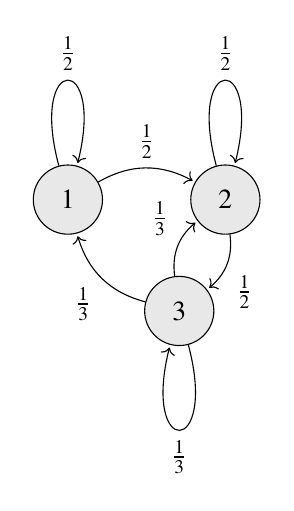
\begin{tikzpicture}[shorten >=1pt,node distance=2cm, scale =3, auto]
			\tikzstyle{every state}=[fill={rgb:black,1;white,10}]
			
			\node[state]   (q_1)                          {$1$};
			\node[state]   (q_2)  [right of=q_1]          {$2$};
			\node[state]   (q_3)  [below right of=q_1]          {$3$};
			
			\path[->]
			(q_1) edge [loop above] node {$\frac{1}{2}$}    (   )
			edge [bend left]  node {$\frac{1}{2}$}    (q_2)
			(q_2) edge [bend left]  node {$\frac{1}{2}$}    (q_3)
			edge [loop above] node {$\frac{1}{2}$}    ()
			(q_3) edge [bend left]  node {$\frac{1}{3}$}    (q_2)
			edge [bend left]  node {$\frac{1}{3}$}    (q_1)
			edge [loop below] node {$\frac{1}{3}$}    ();
		\end{tikzpicture}$
		
		\\  
		&\\
		&\\
		\hline
		\multirow{3}{*}{Checking whether the  } & \\
		& Here,\\chain is Irreducible
		& All the states are accessible to one another. \\and Aperiodic
		& $\implies$ They are in the same communication class. So, it is Irreducible.\\
		& \\
		& There exists the non- zero self-transition, which means that the chain \\
		& is Aperiodic.\\
		&\\ 
		& We know that if the Markov Chain is irreducible and aperiodic then \\
		& \qquad \qquad \qquad $\Vec{\pi}_{j} = \lim_{n \to \infty}P\{X_{n} = j\}$, $j = 1,...,N$ \\
		& These are the stationary probabilities. \\
		&\\
		\hline
		\multirow{3}{*}{Finding the Stationary} & \\
		& Stationary Probability can be represented as\\Probability Distributions
		& \qquad \qquad \qquad $\Vec{\pi} = \Vec{\pi} \vec{P}$\\
		& \\
		& \qquad $\implies$ $\myvec{v_{1}&&v_{2}&&v_{3}} = \myvec{v_{1}&&v_{2}&&v_{3}}\vec{P}$ \\
		& \\
		& Equating the above equation we get \\
		& \\
		& \qquad \qquad \qquad $\frac{1}{2}v_{1}-\frac{1}{3}v_{3} = 0$ $\label{eq:solutions/2018/dec/106/eq}$\\
		& \\
		& \qquad \qquad \qquad $\frac{1}{2}v_{1}-\frac{1}{2}v_{2} + \frac{1}{3}v_{3} = 0$\\
		& \\
		& \qquad \qquad \qquad $\frac{1}{2}v_{2}-\frac{2}{3}v_{3} = 0$\\
		& \\\
		& We see that summation of second and the third equation gives us the \\
		& first equation only. \\
		& And we know that the probability distribution will sum up to 1. \\
		& \\
		& \qquad \qquad \qquad $v_{1}+v_{2}+v_{3} = 1$ \\
		& \\
		& Therefore, we get the equation form as \\
		& \\
		& \qquad \qquad \qquad $\myvec{1&1&1\\\frac{1}{2}&0&\frac{-1}{3}\\\frac{1}{2}&\frac{-1}{2}&\frac{1}{3}}\myvec{v_{1}\\v_{2}\\v_{3}} = \myvec{1\\0\\0}$ \\
		& \\
		\hline
		\multirow{3}{*}{Solving the linear} & \\
		& The above linear equation can be solved using Gauss-Jordan method as\\equtions
		& \\
		& \qquad \qquad \qquad $\myvec{1&1&1&\vrule&1\\\frac{1}{2}&0&\frac{-1}{3}&\vrule&0\\\frac{1}{2}&\frac{-1}{2}&\frac{1}{3}&\vrule&0}$\\
		& \\
		& \qquad $\xleftrightarrow[]{R_2 \leftarrow R_2 - \frac{1}{2}R_1}$
		$\myvec{1&1&1&\vrule&1\\0&\frac{-1}{2}&\frac{-5}{6}&\vrule&\frac{-1}{2}\\\frac{1}{2}&\frac{-1}{2}&\frac{1}{3}&\vrule&0}$\\
		&\\
		& \qquad $\xleftrightarrow[]{R_3 \leftarrow R_3 - \frac{1}{2}R_1}$
		$\myvec{1&1&1&\vrule&1\\0&\frac{-1}{2}&\frac{-5}{6}&\vrule&\frac{-1}{2}\\0&-1&\frac{-1}{6}&\vrule&\frac{-1}{2}}$\\
		&\\
		& \qquad $\xleftrightarrow[]{R_2 \leftarrow \frac{-1}{2}R_2}$
		$\myvec{1&1&1&\vrule&1\\0&1&\frac{5}{3}&\vrule&1\\0&-1&\frac{-1}{6}&\vrule&\frac{-1}{2}}$\\
		&\\
		& \qquad $\xleftrightarrow[]{R_3 \leftarrow R_3 + R_2}$
		$\myvec{1&1&1&\vrule&1\\0&1&\frac{5}{3}&\vrule&1\\0&0&\frac{3}{2}&\vrule&\frac{1}{2}}$\\
		&\\
		& \qquad $\xleftrightarrow[]{R_3 \leftarrow \frac{3}{2}R_3}$
		$\myvec{1&1&1&\vrule&1\\0&1&\frac{5}{3}&\vrule&1\\0&0&1&\vrule&\frac{1}{3}}$\\
		&\\
		& \qquad $\xleftrightarrow[]{R_2 \leftarrow R_2 - \frac{5}{3}R_3}$
		$\myvec{1&1&1&\vrule&1\\0&1&0&\vrule&\frac{4}{9}\\0&0&1&\vrule&\frac{1}{3}}$\\
		&\\
		& \qquad $\xleftrightarrow[]{R_1 \leftarrow R_1 - R_3}$
		$\myvec{1&1&0&\vrule&\frac{2}{3}\\0&1&0&\vrule&\frac{4}{9}\\0&0&1&\vrule&\frac{1}{3}}$\\
		&\\
		& \qquad $\xleftrightarrow[]{R_1 \leftarrow R_1 - R_2}$
		$\myvec{1&0&0&\vrule&\frac{2}{9}\\0&1&0&\vrule&\frac{4}{9}\\0&0&1&\vrule&\frac{1}{3}}$\\
		&\\
		& $\therefore$, stationary probability distribution $\pi$ is given by \\
		& \qquad \qquad $\pi = \myvec{\frac{2}{9} & \frac{4}{9} & \frac{1}{3}}$ \\
		& \\
		\hline
		\multirow{3}{*}{Observations} & \\
		
		
		& Since the given transition probability matrix $\vec{P}$ is irreducible and aperiodic, \\
		& then $\lim_{n \to \infty} \vec{P}^{n}$ converges to a matrix with all rows identical and equal to $\vec{\pi}$. \\
		& \\
		& We were able to find $\vec{\pi}$ as $\myvec{\frac{2}{9} & \frac{4}{9} & \frac{1}{3}}$ \\
		& \\
		& $\lim_{n \to \infty} \vec{P}^{n} = \myvec{\frac{2}{9}&\frac{4}{9}&\frac{1}{3}\\\frac{2}{9}&\frac{4}{9}&\frac{1}{3}\\\frac{2}{9}&\frac{4}{9}&\frac{1}{3}}$\\
		& \\
		& From the above matrix, we get \\
		& \\
		& $\lim_{n \to \infty} \vec{P}^{n}_{11} = \frac{2}{9}$ \\
		&\\
		& $\lim_{n \to \infty} \vec{P}^{n}_{21} = \frac{2}{9}$ \\
		&\\
		& $\lim_{n \to \infty} \vec{P}^{n}_{32} = \frac{4}{9}$ \\
		&\\
		& $\lim_{n \to \infty} \vec{P}^{n}_{13} = \frac{1}{3}$ \\
		&\\
		\hline
		\multirow{3}{*}{Conclusion} & \\
		& From our observation we see that \\
		&\\
		& Options 1) and 4) are True.\\
		& \\
		\hline
\caption{}
\label{eq:solutions/2018/dec/106/table1}
	\end{longtable}
\twocolumn

\item Let $\vec{M}$ be an $n \times n$ Hermitian matrix of rank $k, k \ne n$.  If $\lambda \ne = 0$is an eigenvalue of $\vec{M}$ with corresponding unit column vector $\vec{u}$, then which of the
following are true?
\begin{enumerate}
\item rank$\brak{\vec{M}- \lambda \vec{u}\vec{u}^*} = k-1$.
\item rank$\brak{\vec{M}- \lambda \vec{u}\vec{u}^*} = k$.
\item rank$\brak{\vec{M}- \lambda \vec{u}\vec{u}^*} = k+1$.
\item $\brak{\vec{M}- \lambda \vec{u}\vec{u}^*}^n = \vec{M}^n - \lambda^n \vec{u}\vec{u}^*$.
\end{enumerate}
%
\solution
See Tables \ref{eq:solutions/2018/dec/106/table0} and \ref{eq:solutions/2018/dec/106/table1}


\onecolumn
	\begin{longtable}{|l|l|}
		\hline
		\multirow{3}{*}{Irreducible Markov Chain} 
		& \\
		& A Markov chain is $\textbf{irreducible}$ if all the states communicate with each other,\\
		& i.e., if there is only one communication class.\\
		&\\
		\hline
		\multirow{3}{*}{Aperiodic Markov Chain} & \\
		& If there is a self-transition in the chain ($p^{ii}>0$ for some i), then the chain is\\
		& called as $\textbf{aperiodic}$\\
		& \\
		\hline
		\multirow{3}{*}{Stationary Distribution} & \\
		& A stationary distribution of a Markov chain is a probability distribution that\\
		& remains unchanged in the Markov chain as time progresses. Typically, it is\\
		& represented as a row vector $\Vec{\pi}$ whose entries are probabilities summing to 1,\\ 
		& and given transition matrix $\textbf{P}$, it satisfies\\
		& \\
		&  \qquad \qquad  \qquad$\Vec{\pi} = \Vec{\pi} \textbf{P}$\\
		& \\
		\hline
\caption{}
\label{eq:solutions/2018/dec/106/table0}
	\end{longtable}
	\begin{longtable}{|l|l|}
		\hline
		\multirow{3}{*}{Drawing Transition diagram} 
		& \\
		& 
		
		$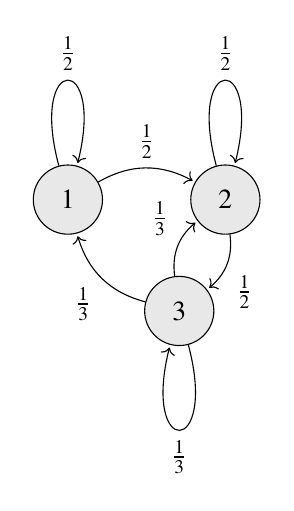
\begin{tikzpicture}[shorten >=1pt,node distance=2cm, scale =3, auto]
			\tikzstyle{every state}=[fill={rgb:black,1;white,10}]
			
			\node[state]   (q_1)                          {$1$};
			\node[state]   (q_2)  [right of=q_1]          {$2$};
			\node[state]   (q_3)  [below right of=q_1]          {$3$};
			
			\path[->]
			(q_1) edge [loop above] node {$\frac{1}{2}$}    (   )
			edge [bend left]  node {$\frac{1}{2}$}    (q_2)
			(q_2) edge [bend left]  node {$\frac{1}{2}$}    (q_3)
			edge [loop above] node {$\frac{1}{2}$}    ()
			(q_3) edge [bend left]  node {$\frac{1}{3}$}    (q_2)
			edge [bend left]  node {$\frac{1}{3}$}    (q_1)
			edge [loop below] node {$\frac{1}{3}$}    ();
		\end{tikzpicture}$
		
		\\  
		&\\
		&\\
		\hline
		\multirow{3}{*}{Checking whether the  } & \\
		& Here,\\chain is Irreducible
		& All the states are accessible to one another. \\and Aperiodic
		& $\implies$ They are in the same communication class. So, it is Irreducible.\\
		& \\
		& There exists the non- zero self-transition, which means that the chain \\
		& is Aperiodic.\\
		&\\ 
		& We know that if the Markov Chain is irreducible and aperiodic then \\
		& \qquad \qquad \qquad $\Vec{\pi}_{j} = \lim_{n \to \infty}P\{X_{n} = j\}$, $j = 1,...,N$ \\
		& These are the stationary probabilities. \\
		&\\
		\hline
		\multirow{3}{*}{Finding the Stationary} & \\
		& Stationary Probability can be represented as\\Probability Distributions
		& \qquad \qquad \qquad $\Vec{\pi} = \Vec{\pi} \vec{P}$\\
		& \\
		& \qquad $\implies$ $\myvec{v_{1}&&v_{2}&&v_{3}} = \myvec{v_{1}&&v_{2}&&v_{3}}\vec{P}$ \\
		& \\
		& Equating the above equation we get \\
		& \\
		& \qquad \qquad \qquad $\frac{1}{2}v_{1}-\frac{1}{3}v_{3} = 0$ $\label{eq:solutions/2018/dec/106/eq}$\\
		& \\
		& \qquad \qquad \qquad $\frac{1}{2}v_{1}-\frac{1}{2}v_{2} + \frac{1}{3}v_{3} = 0$\\
		& \\
		& \qquad \qquad \qquad $\frac{1}{2}v_{2}-\frac{2}{3}v_{3} = 0$\\
		& \\\
		& We see that summation of second and the third equation gives us the \\
		& first equation only. \\
		& And we know that the probability distribution will sum up to 1. \\
		& \\
		& \qquad \qquad \qquad $v_{1}+v_{2}+v_{3} = 1$ \\
		& \\
		& Therefore, we get the equation form as \\
		& \\
		& \qquad \qquad \qquad $\myvec{1&1&1\\\frac{1}{2}&0&\frac{-1}{3}\\\frac{1}{2}&\frac{-1}{2}&\frac{1}{3}}\myvec{v_{1}\\v_{2}\\v_{3}} = \myvec{1\\0\\0}$ \\
		& \\
		\hline
		\multirow{3}{*}{Solving the linear} & \\
		& The above linear equation can be solved using Gauss-Jordan method as\\equtions
		& \\
		& \qquad \qquad \qquad $\myvec{1&1&1&\vrule&1\\\frac{1}{2}&0&\frac{-1}{3}&\vrule&0\\\frac{1}{2}&\frac{-1}{2}&\frac{1}{3}&\vrule&0}$\\
		& \\
		& \qquad $\xleftrightarrow[]{R_2 \leftarrow R_2 - \frac{1}{2}R_1}$
		$\myvec{1&1&1&\vrule&1\\0&\frac{-1}{2}&\frac{-5}{6}&\vrule&\frac{-1}{2}\\\frac{1}{2}&\frac{-1}{2}&\frac{1}{3}&\vrule&0}$\\
		&\\
		& \qquad $\xleftrightarrow[]{R_3 \leftarrow R_3 - \frac{1}{2}R_1}$
		$\myvec{1&1&1&\vrule&1\\0&\frac{-1}{2}&\frac{-5}{6}&\vrule&\frac{-1}{2}\\0&-1&\frac{-1}{6}&\vrule&\frac{-1}{2}}$\\
		&\\
		& \qquad $\xleftrightarrow[]{R_2 \leftarrow \frac{-1}{2}R_2}$
		$\myvec{1&1&1&\vrule&1\\0&1&\frac{5}{3}&\vrule&1\\0&-1&\frac{-1}{6}&\vrule&\frac{-1}{2}}$\\
		&\\
		& \qquad $\xleftrightarrow[]{R_3 \leftarrow R_3 + R_2}$
		$\myvec{1&1&1&\vrule&1\\0&1&\frac{5}{3}&\vrule&1\\0&0&\frac{3}{2}&\vrule&\frac{1}{2}}$\\
		&\\
		& \qquad $\xleftrightarrow[]{R_3 \leftarrow \frac{3}{2}R_3}$
		$\myvec{1&1&1&\vrule&1\\0&1&\frac{5}{3}&\vrule&1\\0&0&1&\vrule&\frac{1}{3}}$\\
		&\\
		& \qquad $\xleftrightarrow[]{R_2 \leftarrow R_2 - \frac{5}{3}R_3}$
		$\myvec{1&1&1&\vrule&1\\0&1&0&\vrule&\frac{4}{9}\\0&0&1&\vrule&\frac{1}{3}}$\\
		&\\
		& \qquad $\xleftrightarrow[]{R_1 \leftarrow R_1 - R_3}$
		$\myvec{1&1&0&\vrule&\frac{2}{3}\\0&1&0&\vrule&\frac{4}{9}\\0&0&1&\vrule&\frac{1}{3}}$\\
		&\\
		& \qquad $\xleftrightarrow[]{R_1 \leftarrow R_1 - R_2}$
		$\myvec{1&0&0&\vrule&\frac{2}{9}\\0&1&0&\vrule&\frac{4}{9}\\0&0&1&\vrule&\frac{1}{3}}$\\
		&\\
		& $\therefore$, stationary probability distribution $\pi$ is given by \\
		& \qquad \qquad $\pi = \myvec{\frac{2}{9} & \frac{4}{9} & \frac{1}{3}}$ \\
		& \\
		\hline
		\multirow{3}{*}{Observations} & \\
		
		
		& Since the given transition probability matrix $\vec{P}$ is irreducible and aperiodic, \\
		& then $\lim_{n \to \infty} \vec{P}^{n}$ converges to a matrix with all rows identical and equal to $\vec{\pi}$. \\
		& \\
		& We were able to find $\vec{\pi}$ as $\myvec{\frac{2}{9} & \frac{4}{9} & \frac{1}{3}}$ \\
		& \\
		& $\lim_{n \to \infty} \vec{P}^{n} = \myvec{\frac{2}{9}&\frac{4}{9}&\frac{1}{3}\\\frac{2}{9}&\frac{4}{9}&\frac{1}{3}\\\frac{2}{9}&\frac{4}{9}&\frac{1}{3}}$\\
		& \\
		& From the above matrix, we get \\
		& \\
		& $\lim_{n \to \infty} \vec{P}^{n}_{11} = \frac{2}{9}$ \\
		&\\
		& $\lim_{n \to \infty} \vec{P}^{n}_{21} = \frac{2}{9}$ \\
		&\\
		& $\lim_{n \to \infty} \vec{P}^{n}_{32} = \frac{4}{9}$ \\
		&\\
		& $\lim_{n \to \infty} \vec{P}^{n}_{13} = \frac{1}{3}$ \\
		&\\
		\hline
		\multirow{3}{*}{Conclusion} & \\
		& From our observation we see that \\
		&\\
		& Options 1) and 4) are True.\\
		& \\
		\hline
\caption{}
\label{eq:solutions/2018/dec/106/table1}
	\end{longtable}
\twocolumn

\item Define a real valued function $B$ on $\mathbb{R}^2 \times \mathbb{R}^2 $ as 
\begin{align}
B\brak{\vec{x},\vec{y}} = x_1y_1 - x_1y_2-x_2y_1+4x_2y_2
\end{align}
Let $\vec{v}_0 = \myvec{1\\0}$ and 
\begin{align}
W = \cbrak{\vec{v} \in \mathbb{R}^2: B(\vec{v}_0,\vec{v}) =0}
\end{align}
Then $W$
\begin{enumerate}
\item is not a subspace of $\mathbb{R}^2$.
\item equals $\vec{0}$.
\item is the y axis
\item is the line passing through $\myvec{0 \\ 0}$ and $\myvec{1 \\ 1}$.
\end{enumerate}
%
\solution
See Tables \ref{eq:solutions/2018/dec/106/table0} and \ref{eq:solutions/2018/dec/106/table1}


\onecolumn
	\begin{longtable}{|l|l|}
		\hline
		\multirow{3}{*}{Irreducible Markov Chain} 
		& \\
		& A Markov chain is $\textbf{irreducible}$ if all the states communicate with each other,\\
		& i.e., if there is only one communication class.\\
		&\\
		\hline
		\multirow{3}{*}{Aperiodic Markov Chain} & \\
		& If there is a self-transition in the chain ($p^{ii}>0$ for some i), then the chain is\\
		& called as $\textbf{aperiodic}$\\
		& \\
		\hline
		\multirow{3}{*}{Stationary Distribution} & \\
		& A stationary distribution of a Markov chain is a probability distribution that\\
		& remains unchanged in the Markov chain as time progresses. Typically, it is\\
		& represented as a row vector $\Vec{\pi}$ whose entries are probabilities summing to 1,\\ 
		& and given transition matrix $\textbf{P}$, it satisfies\\
		& \\
		&  \qquad \qquad  \qquad$\Vec{\pi} = \Vec{\pi} \textbf{P}$\\
		& \\
		\hline
\caption{}
\label{eq:solutions/2018/dec/106/table0}
	\end{longtable}
	\begin{longtable}{|l|l|}
		\hline
		\multirow{3}{*}{Drawing Transition diagram} 
		& \\
		& 
		
		$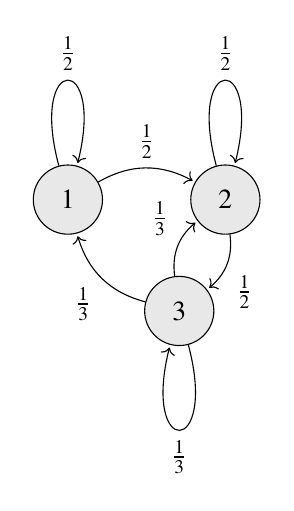
\begin{tikzpicture}[shorten >=1pt,node distance=2cm, scale =3, auto]
			\tikzstyle{every state}=[fill={rgb:black,1;white,10}]
			
			\node[state]   (q_1)                          {$1$};
			\node[state]   (q_2)  [right of=q_1]          {$2$};
			\node[state]   (q_3)  [below right of=q_1]          {$3$};
			
			\path[->]
			(q_1) edge [loop above] node {$\frac{1}{2}$}    (   )
			edge [bend left]  node {$\frac{1}{2}$}    (q_2)
			(q_2) edge [bend left]  node {$\frac{1}{2}$}    (q_3)
			edge [loop above] node {$\frac{1}{2}$}    ()
			(q_3) edge [bend left]  node {$\frac{1}{3}$}    (q_2)
			edge [bend left]  node {$\frac{1}{3}$}    (q_1)
			edge [loop below] node {$\frac{1}{3}$}    ();
		\end{tikzpicture}$
		
		\\  
		&\\
		&\\
		\hline
		\multirow{3}{*}{Checking whether the  } & \\
		& Here,\\chain is Irreducible
		& All the states are accessible to one another. \\and Aperiodic
		& $\implies$ They are in the same communication class. So, it is Irreducible.\\
		& \\
		& There exists the non- zero self-transition, which means that the chain \\
		& is Aperiodic.\\
		&\\ 
		& We know that if the Markov Chain is irreducible and aperiodic then \\
		& \qquad \qquad \qquad $\Vec{\pi}_{j} = \lim_{n \to \infty}P\{X_{n} = j\}$, $j = 1,...,N$ \\
		& These are the stationary probabilities. \\
		&\\
		\hline
		\multirow{3}{*}{Finding the Stationary} & \\
		& Stationary Probability can be represented as\\Probability Distributions
		& \qquad \qquad \qquad $\Vec{\pi} = \Vec{\pi} \vec{P}$\\
		& \\
		& \qquad $\implies$ $\myvec{v_{1}&&v_{2}&&v_{3}} = \myvec{v_{1}&&v_{2}&&v_{3}}\vec{P}$ \\
		& \\
		& Equating the above equation we get \\
		& \\
		& \qquad \qquad \qquad $\frac{1}{2}v_{1}-\frac{1}{3}v_{3} = 0$ $\label{eq:solutions/2018/dec/106/eq}$\\
		& \\
		& \qquad \qquad \qquad $\frac{1}{2}v_{1}-\frac{1}{2}v_{2} + \frac{1}{3}v_{3} = 0$\\
		& \\
		& \qquad \qquad \qquad $\frac{1}{2}v_{2}-\frac{2}{3}v_{3} = 0$\\
		& \\\
		& We see that summation of second and the third equation gives us the \\
		& first equation only. \\
		& And we know that the probability distribution will sum up to 1. \\
		& \\
		& \qquad \qquad \qquad $v_{1}+v_{2}+v_{3} = 1$ \\
		& \\
		& Therefore, we get the equation form as \\
		& \\
		& \qquad \qquad \qquad $\myvec{1&1&1\\\frac{1}{2}&0&\frac{-1}{3}\\\frac{1}{2}&\frac{-1}{2}&\frac{1}{3}}\myvec{v_{1}\\v_{2}\\v_{3}} = \myvec{1\\0\\0}$ \\
		& \\
		\hline
		\multirow{3}{*}{Solving the linear} & \\
		& The above linear equation can be solved using Gauss-Jordan method as\\equtions
		& \\
		& \qquad \qquad \qquad $\myvec{1&1&1&\vrule&1\\\frac{1}{2}&0&\frac{-1}{3}&\vrule&0\\\frac{1}{2}&\frac{-1}{2}&\frac{1}{3}&\vrule&0}$\\
		& \\
		& \qquad $\xleftrightarrow[]{R_2 \leftarrow R_2 - \frac{1}{2}R_1}$
		$\myvec{1&1&1&\vrule&1\\0&\frac{-1}{2}&\frac{-5}{6}&\vrule&\frac{-1}{2}\\\frac{1}{2}&\frac{-1}{2}&\frac{1}{3}&\vrule&0}$\\
		&\\
		& \qquad $\xleftrightarrow[]{R_3 \leftarrow R_3 - \frac{1}{2}R_1}$
		$\myvec{1&1&1&\vrule&1\\0&\frac{-1}{2}&\frac{-5}{6}&\vrule&\frac{-1}{2}\\0&-1&\frac{-1}{6}&\vrule&\frac{-1}{2}}$\\
		&\\
		& \qquad $\xleftrightarrow[]{R_2 \leftarrow \frac{-1}{2}R_2}$
		$\myvec{1&1&1&\vrule&1\\0&1&\frac{5}{3}&\vrule&1\\0&-1&\frac{-1}{6}&\vrule&\frac{-1}{2}}$\\
		&\\
		& \qquad $\xleftrightarrow[]{R_3 \leftarrow R_3 + R_2}$
		$\myvec{1&1&1&\vrule&1\\0&1&\frac{5}{3}&\vrule&1\\0&0&\frac{3}{2}&\vrule&\frac{1}{2}}$\\
		&\\
		& \qquad $\xleftrightarrow[]{R_3 \leftarrow \frac{3}{2}R_3}$
		$\myvec{1&1&1&\vrule&1\\0&1&\frac{5}{3}&\vrule&1\\0&0&1&\vrule&\frac{1}{3}}$\\
		&\\
		& \qquad $\xleftrightarrow[]{R_2 \leftarrow R_2 - \frac{5}{3}R_3}$
		$\myvec{1&1&1&\vrule&1\\0&1&0&\vrule&\frac{4}{9}\\0&0&1&\vrule&\frac{1}{3}}$\\
		&\\
		& \qquad $\xleftrightarrow[]{R_1 \leftarrow R_1 - R_3}$
		$\myvec{1&1&0&\vrule&\frac{2}{3}\\0&1&0&\vrule&\frac{4}{9}\\0&0&1&\vrule&\frac{1}{3}}$\\
		&\\
		& \qquad $\xleftrightarrow[]{R_1 \leftarrow R_1 - R_2}$
		$\myvec{1&0&0&\vrule&\frac{2}{9}\\0&1&0&\vrule&\frac{4}{9}\\0&0&1&\vrule&\frac{1}{3}}$\\
		&\\
		& $\therefore$, stationary probability distribution $\pi$ is given by \\
		& \qquad \qquad $\pi = \myvec{\frac{2}{9} & \frac{4}{9} & \frac{1}{3}}$ \\
		& \\
		\hline
		\multirow{3}{*}{Observations} & \\
		
		
		& Since the given transition probability matrix $\vec{P}$ is irreducible and aperiodic, \\
		& then $\lim_{n \to \infty} \vec{P}^{n}$ converges to a matrix with all rows identical and equal to $\vec{\pi}$. \\
		& \\
		& We were able to find $\vec{\pi}$ as $\myvec{\frac{2}{9} & \frac{4}{9} & \frac{1}{3}}$ \\
		& \\
		& $\lim_{n \to \infty} \vec{P}^{n} = \myvec{\frac{2}{9}&\frac{4}{9}&\frac{1}{3}\\\frac{2}{9}&\frac{4}{9}&\frac{1}{3}\\\frac{2}{9}&\frac{4}{9}&\frac{1}{3}}$\\
		& \\
		& From the above matrix, we get \\
		& \\
		& $\lim_{n \to \infty} \vec{P}^{n}_{11} = \frac{2}{9}$ \\
		&\\
		& $\lim_{n \to \infty} \vec{P}^{n}_{21} = \frac{2}{9}$ \\
		&\\
		& $\lim_{n \to \infty} \vec{P}^{n}_{32} = \frac{4}{9}$ \\
		&\\
		& $\lim_{n \to \infty} \vec{P}^{n}_{13} = \frac{1}{3}$ \\
		&\\
		\hline
		\multirow{3}{*}{Conclusion} & \\
		& From our observation we see that \\
		&\\
		& Options 1) and 4) are True.\\
		& \\
		\hline
\caption{}
\label{eq:solutions/2018/dec/106/table1}
	\end{longtable}
\twocolumn

\item Consider the Quadratic forms
\begin{align}
Q_1(x,y) = xy
\\
Q_2(x,y) = x^2+2xy+y^2
\\
Q_3(x,y) = x^2+3xy+2y^2
\end{align}
%
on $\mathbb{R}^2$.  Choose the correct statements from below
\begin{enumerate}
\item $Q_1$ and $Q_2$ are equivalent.
\item $Q_1$ and $Q_3$ are equivalent.
\item $Q_2$ and $Q_3$ are equivalent.
\item all are equivalent.
\end{enumerate}
\solution
See Tables \ref{eq:solutions/2018/dec/106/table0} and \ref{eq:solutions/2018/dec/106/table1}


\onecolumn
	\begin{longtable}{|l|l|}
		\hline
		\multirow{3}{*}{Irreducible Markov Chain} 
		& \\
		& A Markov chain is $\textbf{irreducible}$ if all the states communicate with each other,\\
		& i.e., if there is only one communication class.\\
		&\\
		\hline
		\multirow{3}{*}{Aperiodic Markov Chain} & \\
		& If there is a self-transition in the chain ($p^{ii}>0$ for some i), then the chain is\\
		& called as $\textbf{aperiodic}$\\
		& \\
		\hline
		\multirow{3}{*}{Stationary Distribution} & \\
		& A stationary distribution of a Markov chain is a probability distribution that\\
		& remains unchanged in the Markov chain as time progresses. Typically, it is\\
		& represented as a row vector $\Vec{\pi}$ whose entries are probabilities summing to 1,\\ 
		& and given transition matrix $\textbf{P}$, it satisfies\\
		& \\
		&  \qquad \qquad  \qquad$\Vec{\pi} = \Vec{\pi} \textbf{P}$\\
		& \\
		\hline
\caption{}
\label{eq:solutions/2018/dec/106/table0}
	\end{longtable}
	\begin{longtable}{|l|l|}
		\hline
		\multirow{3}{*}{Drawing Transition diagram} 
		& \\
		& 
		
		$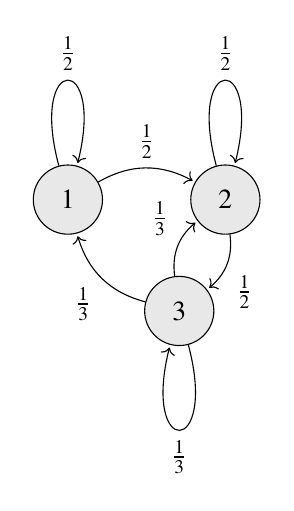
\begin{tikzpicture}[shorten >=1pt,node distance=2cm, scale =3, auto]
			\tikzstyle{every state}=[fill={rgb:black,1;white,10}]
			
			\node[state]   (q_1)                          {$1$};
			\node[state]   (q_2)  [right of=q_1]          {$2$};
			\node[state]   (q_3)  [below right of=q_1]          {$3$};
			
			\path[->]
			(q_1) edge [loop above] node {$\frac{1}{2}$}    (   )
			edge [bend left]  node {$\frac{1}{2}$}    (q_2)
			(q_2) edge [bend left]  node {$\frac{1}{2}$}    (q_3)
			edge [loop above] node {$\frac{1}{2}$}    ()
			(q_3) edge [bend left]  node {$\frac{1}{3}$}    (q_2)
			edge [bend left]  node {$\frac{1}{3}$}    (q_1)
			edge [loop below] node {$\frac{1}{3}$}    ();
		\end{tikzpicture}$
		
		\\  
		&\\
		&\\
		\hline
		\multirow{3}{*}{Checking whether the  } & \\
		& Here,\\chain is Irreducible
		& All the states are accessible to one another. \\and Aperiodic
		& $\implies$ They are in the same communication class. So, it is Irreducible.\\
		& \\
		& There exists the non- zero self-transition, which means that the chain \\
		& is Aperiodic.\\
		&\\ 
		& We know that if the Markov Chain is irreducible and aperiodic then \\
		& \qquad \qquad \qquad $\Vec{\pi}_{j} = \lim_{n \to \infty}P\{X_{n} = j\}$, $j = 1,...,N$ \\
		& These are the stationary probabilities. \\
		&\\
		\hline
		\multirow{3}{*}{Finding the Stationary} & \\
		& Stationary Probability can be represented as\\Probability Distributions
		& \qquad \qquad \qquad $\Vec{\pi} = \Vec{\pi} \vec{P}$\\
		& \\
		& \qquad $\implies$ $\myvec{v_{1}&&v_{2}&&v_{3}} = \myvec{v_{1}&&v_{2}&&v_{3}}\vec{P}$ \\
		& \\
		& Equating the above equation we get \\
		& \\
		& \qquad \qquad \qquad $\frac{1}{2}v_{1}-\frac{1}{3}v_{3} = 0$ $\label{eq:solutions/2018/dec/106/eq}$\\
		& \\
		& \qquad \qquad \qquad $\frac{1}{2}v_{1}-\frac{1}{2}v_{2} + \frac{1}{3}v_{3} = 0$\\
		& \\
		& \qquad \qquad \qquad $\frac{1}{2}v_{2}-\frac{2}{3}v_{3} = 0$\\
		& \\\
		& We see that summation of second and the third equation gives us the \\
		& first equation only. \\
		& And we know that the probability distribution will sum up to 1. \\
		& \\
		& \qquad \qquad \qquad $v_{1}+v_{2}+v_{3} = 1$ \\
		& \\
		& Therefore, we get the equation form as \\
		& \\
		& \qquad \qquad \qquad $\myvec{1&1&1\\\frac{1}{2}&0&\frac{-1}{3}\\\frac{1}{2}&\frac{-1}{2}&\frac{1}{3}}\myvec{v_{1}\\v_{2}\\v_{3}} = \myvec{1\\0\\0}$ \\
		& \\
		\hline
		\multirow{3}{*}{Solving the linear} & \\
		& The above linear equation can be solved using Gauss-Jordan method as\\equtions
		& \\
		& \qquad \qquad \qquad $\myvec{1&1&1&\vrule&1\\\frac{1}{2}&0&\frac{-1}{3}&\vrule&0\\\frac{1}{2}&\frac{-1}{2}&\frac{1}{3}&\vrule&0}$\\
		& \\
		& \qquad $\xleftrightarrow[]{R_2 \leftarrow R_2 - \frac{1}{2}R_1}$
		$\myvec{1&1&1&\vrule&1\\0&\frac{-1}{2}&\frac{-5}{6}&\vrule&\frac{-1}{2}\\\frac{1}{2}&\frac{-1}{2}&\frac{1}{3}&\vrule&0}$\\
		&\\
		& \qquad $\xleftrightarrow[]{R_3 \leftarrow R_3 - \frac{1}{2}R_1}$
		$\myvec{1&1&1&\vrule&1\\0&\frac{-1}{2}&\frac{-5}{6}&\vrule&\frac{-1}{2}\\0&-1&\frac{-1}{6}&\vrule&\frac{-1}{2}}$\\
		&\\
		& \qquad $\xleftrightarrow[]{R_2 \leftarrow \frac{-1}{2}R_2}$
		$\myvec{1&1&1&\vrule&1\\0&1&\frac{5}{3}&\vrule&1\\0&-1&\frac{-1}{6}&\vrule&\frac{-1}{2}}$\\
		&\\
		& \qquad $\xleftrightarrow[]{R_3 \leftarrow R_3 + R_2}$
		$\myvec{1&1&1&\vrule&1\\0&1&\frac{5}{3}&\vrule&1\\0&0&\frac{3}{2}&\vrule&\frac{1}{2}}$\\
		&\\
		& \qquad $\xleftrightarrow[]{R_3 \leftarrow \frac{3}{2}R_3}$
		$\myvec{1&1&1&\vrule&1\\0&1&\frac{5}{3}&\vrule&1\\0&0&1&\vrule&\frac{1}{3}}$\\
		&\\
		& \qquad $\xleftrightarrow[]{R_2 \leftarrow R_2 - \frac{5}{3}R_3}$
		$\myvec{1&1&1&\vrule&1\\0&1&0&\vrule&\frac{4}{9}\\0&0&1&\vrule&\frac{1}{3}}$\\
		&\\
		& \qquad $\xleftrightarrow[]{R_1 \leftarrow R_1 - R_3}$
		$\myvec{1&1&0&\vrule&\frac{2}{3}\\0&1&0&\vrule&\frac{4}{9}\\0&0&1&\vrule&\frac{1}{3}}$\\
		&\\
		& \qquad $\xleftrightarrow[]{R_1 \leftarrow R_1 - R_2}$
		$\myvec{1&0&0&\vrule&\frac{2}{9}\\0&1&0&\vrule&\frac{4}{9}\\0&0&1&\vrule&\frac{1}{3}}$\\
		&\\
		& $\therefore$, stationary probability distribution $\pi$ is given by \\
		& \qquad \qquad $\pi = \myvec{\frac{2}{9} & \frac{4}{9} & \frac{1}{3}}$ \\
		& \\
		\hline
		\multirow{3}{*}{Observations} & \\
		
		
		& Since the given transition probability matrix $\vec{P}$ is irreducible and aperiodic, \\
		& then $\lim_{n \to \infty} \vec{P}^{n}$ converges to a matrix with all rows identical and equal to $\vec{\pi}$. \\
		& \\
		& We were able to find $\vec{\pi}$ as $\myvec{\frac{2}{9} & \frac{4}{9} & \frac{1}{3}}$ \\
		& \\
		& $\lim_{n \to \infty} \vec{P}^{n} = \myvec{\frac{2}{9}&\frac{4}{9}&\frac{1}{3}\\\frac{2}{9}&\frac{4}{9}&\frac{1}{3}\\\frac{2}{9}&\frac{4}{9}&\frac{1}{3}}$\\
		& \\
		& From the above matrix, we get \\
		& \\
		& $\lim_{n \to \infty} \vec{P}^{n}_{11} = \frac{2}{9}$ \\
		&\\
		& $\lim_{n \to \infty} \vec{P}^{n}_{21} = \frac{2}{9}$ \\
		&\\
		& $\lim_{n \to \infty} \vec{P}^{n}_{32} = \frac{4}{9}$ \\
		&\\
		& $\lim_{n \to \infty} \vec{P}^{n}_{13} = \frac{1}{3}$ \\
		&\\
		\hline
		\multirow{3}{*}{Conclusion} & \\
		& From our observation we see that \\
		&\\
		& Options 1) and 4) are True.\\
		& \\
		\hline
\caption{}
\label{eq:solutions/2018/dec/106/table1}
	\end{longtable}
\twocolumn

\item Consider a Markov Chain with state space $\cbrak{0,1,2}$ and transition matrix
\begin{align}
P = 
\begin{blockarray}{c@{\hspace{1pt}}rrr@{\hspace{3pt}}}
         & 0   & 1   & 2 \\
        \begin{block}{r@{\hspace{3pt}}@{\hspace{1pt}}
    (@{\hspace{1pt}}rrr@{\hspace{1pt}}@{\hspace{1pt}})}
        0 & \frac{1}{2} & \frac{1}{2} & 0  \\
        1 & 0 &\frac{1}{2}  & \frac{3}{4}  \\
%
        2 &  \frac{1}{3} & \frac{1}{3} & \frac{1}{3}  \\
        \end{block}
    \end{blockarray}
\end{align}
For any two states $i$ and $j$, let $p_{ij}^{(n)}$ denote the $n$-step transition probability of going from $i$ to $j$.  Identify correct statements.
\begin{enumerate}
\item $\lim_{n \to \infty} p_{11}^{(n)} = \frac{2}{9}$
\item $\lim_{n \to \infty} p_{21}^{(n)} = 0$
\item $\lim_{n \to \infty} p_{32}^{(n)} = \frac{1}{3}$
\item $\lim_{n \to \infty} p_{13}^{(n)} = \frac{1}{3}$
\end{enumerate}
\solution
See Tables \ref{eq:solutions/2018/dec/106/table0} and \ref{eq:solutions/2018/dec/106/table1}


\onecolumn
	\begin{longtable}{|l|l|}
		\hline
		\multirow{3}{*}{Irreducible Markov Chain} 
		& \\
		& A Markov chain is $\textbf{irreducible}$ if all the states communicate with each other,\\
		& i.e., if there is only one communication class.\\
		&\\
		\hline
		\multirow{3}{*}{Aperiodic Markov Chain} & \\
		& If there is a self-transition in the chain ($p^{ii}>0$ for some i), then the chain is\\
		& called as $\textbf{aperiodic}$\\
		& \\
		\hline
		\multirow{3}{*}{Stationary Distribution} & \\
		& A stationary distribution of a Markov chain is a probability distribution that\\
		& remains unchanged in the Markov chain as time progresses. Typically, it is\\
		& represented as a row vector $\Vec{\pi}$ whose entries are probabilities summing to 1,\\ 
		& and given transition matrix $\textbf{P}$, it satisfies\\
		& \\
		&  \qquad \qquad  \qquad$\Vec{\pi} = \Vec{\pi} \textbf{P}$\\
		& \\
		\hline
\caption{}
\label{eq:solutions/2018/dec/106/table0}
	\end{longtable}
	\begin{longtable}{|l|l|}
		\hline
		\multirow{3}{*}{Drawing Transition diagram} 
		& \\
		& 
		
		$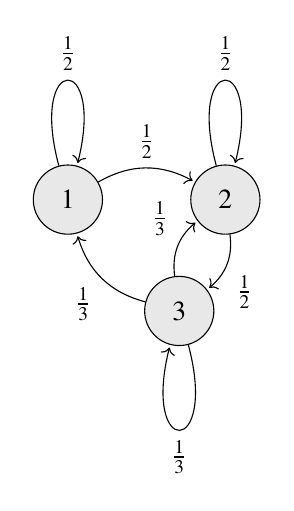
\begin{tikzpicture}[shorten >=1pt,node distance=2cm, scale =3, auto]
			\tikzstyle{every state}=[fill={rgb:black,1;white,10}]
			
			\node[state]   (q_1)                          {$1$};
			\node[state]   (q_2)  [right of=q_1]          {$2$};
			\node[state]   (q_3)  [below right of=q_1]          {$3$};
			
			\path[->]
			(q_1) edge [loop above] node {$\frac{1}{2}$}    (   )
			edge [bend left]  node {$\frac{1}{2}$}    (q_2)
			(q_2) edge [bend left]  node {$\frac{1}{2}$}    (q_3)
			edge [loop above] node {$\frac{1}{2}$}    ()
			(q_3) edge [bend left]  node {$\frac{1}{3}$}    (q_2)
			edge [bend left]  node {$\frac{1}{3}$}    (q_1)
			edge [loop below] node {$\frac{1}{3}$}    ();
		\end{tikzpicture}$
		
		\\  
		&\\
		&\\
		\hline
		\multirow{3}{*}{Checking whether the  } & \\
		& Here,\\chain is Irreducible
		& All the states are accessible to one another. \\and Aperiodic
		& $\implies$ They are in the same communication class. So, it is Irreducible.\\
		& \\
		& There exists the non- zero self-transition, which means that the chain \\
		& is Aperiodic.\\
		&\\ 
		& We know that if the Markov Chain is irreducible and aperiodic then \\
		& \qquad \qquad \qquad $\Vec{\pi}_{j} = \lim_{n \to \infty}P\{X_{n} = j\}$, $j = 1,...,N$ \\
		& These are the stationary probabilities. \\
		&\\
		\hline
		\multirow{3}{*}{Finding the Stationary} & \\
		& Stationary Probability can be represented as\\Probability Distributions
		& \qquad \qquad \qquad $\Vec{\pi} = \Vec{\pi} \vec{P}$\\
		& \\
		& \qquad $\implies$ $\myvec{v_{1}&&v_{2}&&v_{3}} = \myvec{v_{1}&&v_{2}&&v_{3}}\vec{P}$ \\
		& \\
		& Equating the above equation we get \\
		& \\
		& \qquad \qquad \qquad $\frac{1}{2}v_{1}-\frac{1}{3}v_{3} = 0$ $\label{eq:solutions/2018/dec/106/eq}$\\
		& \\
		& \qquad \qquad \qquad $\frac{1}{2}v_{1}-\frac{1}{2}v_{2} + \frac{1}{3}v_{3} = 0$\\
		& \\
		& \qquad \qquad \qquad $\frac{1}{2}v_{2}-\frac{2}{3}v_{3} = 0$\\
		& \\\
		& We see that summation of second and the third equation gives us the \\
		& first equation only. \\
		& And we know that the probability distribution will sum up to 1. \\
		& \\
		& \qquad \qquad \qquad $v_{1}+v_{2}+v_{3} = 1$ \\
		& \\
		& Therefore, we get the equation form as \\
		& \\
		& \qquad \qquad \qquad $\myvec{1&1&1\\\frac{1}{2}&0&\frac{-1}{3}\\\frac{1}{2}&\frac{-1}{2}&\frac{1}{3}}\myvec{v_{1}\\v_{2}\\v_{3}} = \myvec{1\\0\\0}$ \\
		& \\
		\hline
		\multirow{3}{*}{Solving the linear} & \\
		& The above linear equation can be solved using Gauss-Jordan method as\\equtions
		& \\
		& \qquad \qquad \qquad $\myvec{1&1&1&\vrule&1\\\frac{1}{2}&0&\frac{-1}{3}&\vrule&0\\\frac{1}{2}&\frac{-1}{2}&\frac{1}{3}&\vrule&0}$\\
		& \\
		& \qquad $\xleftrightarrow[]{R_2 \leftarrow R_2 - \frac{1}{2}R_1}$
		$\myvec{1&1&1&\vrule&1\\0&\frac{-1}{2}&\frac{-5}{6}&\vrule&\frac{-1}{2}\\\frac{1}{2}&\frac{-1}{2}&\frac{1}{3}&\vrule&0}$\\
		&\\
		& \qquad $\xleftrightarrow[]{R_3 \leftarrow R_3 - \frac{1}{2}R_1}$
		$\myvec{1&1&1&\vrule&1\\0&\frac{-1}{2}&\frac{-5}{6}&\vrule&\frac{-1}{2}\\0&-1&\frac{-1}{6}&\vrule&\frac{-1}{2}}$\\
		&\\
		& \qquad $\xleftrightarrow[]{R_2 \leftarrow \frac{-1}{2}R_2}$
		$\myvec{1&1&1&\vrule&1\\0&1&\frac{5}{3}&\vrule&1\\0&-1&\frac{-1}{6}&\vrule&\frac{-1}{2}}$\\
		&\\
		& \qquad $\xleftrightarrow[]{R_3 \leftarrow R_3 + R_2}$
		$\myvec{1&1&1&\vrule&1\\0&1&\frac{5}{3}&\vrule&1\\0&0&\frac{3}{2}&\vrule&\frac{1}{2}}$\\
		&\\
		& \qquad $\xleftrightarrow[]{R_3 \leftarrow \frac{3}{2}R_3}$
		$\myvec{1&1&1&\vrule&1\\0&1&\frac{5}{3}&\vrule&1\\0&0&1&\vrule&\frac{1}{3}}$\\
		&\\
		& \qquad $\xleftrightarrow[]{R_2 \leftarrow R_2 - \frac{5}{3}R_3}$
		$\myvec{1&1&1&\vrule&1\\0&1&0&\vrule&\frac{4}{9}\\0&0&1&\vrule&\frac{1}{3}}$\\
		&\\
		& \qquad $\xleftrightarrow[]{R_1 \leftarrow R_1 - R_3}$
		$\myvec{1&1&0&\vrule&\frac{2}{3}\\0&1&0&\vrule&\frac{4}{9}\\0&0&1&\vrule&\frac{1}{3}}$\\
		&\\
		& \qquad $\xleftrightarrow[]{R_1 \leftarrow R_1 - R_2}$
		$\myvec{1&0&0&\vrule&\frac{2}{9}\\0&1&0&\vrule&\frac{4}{9}\\0&0&1&\vrule&\frac{1}{3}}$\\
		&\\
		& $\therefore$, stationary probability distribution $\pi$ is given by \\
		& \qquad \qquad $\pi = \myvec{\frac{2}{9} & \frac{4}{9} & \frac{1}{3}}$ \\
		& \\
		\hline
		\multirow{3}{*}{Observations} & \\
		
		
		& Since the given transition probability matrix $\vec{P}$ is irreducible and aperiodic, \\
		& then $\lim_{n \to \infty} \vec{P}^{n}$ converges to a matrix with all rows identical and equal to $\vec{\pi}$. \\
		& \\
		& We were able to find $\vec{\pi}$ as $\myvec{\frac{2}{9} & \frac{4}{9} & \frac{1}{3}}$ \\
		& \\
		& $\lim_{n \to \infty} \vec{P}^{n} = \myvec{\frac{2}{9}&\frac{4}{9}&\frac{1}{3}\\\frac{2}{9}&\frac{4}{9}&\frac{1}{3}\\\frac{2}{9}&\frac{4}{9}&\frac{1}{3}}$\\
		& \\
		& From the above matrix, we get \\
		& \\
		& $\lim_{n \to \infty} \vec{P}^{n}_{11} = \frac{2}{9}$ \\
		&\\
		& $\lim_{n \to \infty} \vec{P}^{n}_{21} = \frac{2}{9}$ \\
		&\\
		& $\lim_{n \to \infty} \vec{P}^{n}_{32} = \frac{4}{9}$ \\
		&\\
		& $\lim_{n \to \infty} \vec{P}^{n}_{13} = \frac{1}{3}$ \\
		&\\
		\hline
		\multirow{3}{*}{Conclusion} & \\
		& From our observation we see that \\
		&\\
		& Options 1) and 4) are True.\\
		& \\
		\hline
\caption{}
\label{eq:solutions/2018/dec/106/table1}
	\end{longtable}
\twocolumn


\end{enumerate}

\twocolumn
\section{June 2017}
\renewcommand{\theequation}{\theenumi}
\renewcommand{\thefigure}{\theenumi}
\begin{enumerate}[label=\thesection.\arabic*.,ref=\thesection.\theenumi]
\numberwithin{equation}{enumi}
\numberwithin{figure}{enumi}

\item 	Let $\vec{A}$ be a $4 \times 4$ matrix. Suppose that the null space $N(\vec{A})$ of $\vec{A}$ is
	\begin{align}
		\cbrak{(x,y,z,w) \in \vec{R}^4 : x + y + z = 0 , x + y + w = 0}
	\end{align}
Then which one of the following is correct
\begin{enumerate}
\item  dim(column space$(\vec{A})) = 1$ 
\item dim(column space$(\vec{A})) = 2$
\item rank$(\vec{A}) = 1$
\item $\vec{S}= \cbrak{(1, 1, 1, 0), (1, 1, 0, 1)}$ is a basis of $N(\vec{A})$
\end{enumerate}
%
%
\solution
See Tables \ref{eq:solutions/2018/dec/106/table0} and \ref{eq:solutions/2018/dec/106/table1}


\onecolumn
	\begin{longtable}{|l|l|}
		\hline
		\multirow{3}{*}{Irreducible Markov Chain} 
		& \\
		& A Markov chain is $\textbf{irreducible}$ if all the states communicate with each other,\\
		& i.e., if there is only one communication class.\\
		&\\
		\hline
		\multirow{3}{*}{Aperiodic Markov Chain} & \\
		& If there is a self-transition in the chain ($p^{ii}>0$ for some i), then the chain is\\
		& called as $\textbf{aperiodic}$\\
		& \\
		\hline
		\multirow{3}{*}{Stationary Distribution} & \\
		& A stationary distribution of a Markov chain is a probability distribution that\\
		& remains unchanged in the Markov chain as time progresses. Typically, it is\\
		& represented as a row vector $\Vec{\pi}$ whose entries are probabilities summing to 1,\\ 
		& and given transition matrix $\textbf{P}$, it satisfies\\
		& \\
		&  \qquad \qquad  \qquad$\Vec{\pi} = \Vec{\pi} \textbf{P}$\\
		& \\
		\hline
\caption{}
\label{eq:solutions/2018/dec/106/table0}
	\end{longtable}
	\begin{longtable}{|l|l|}
		\hline
		\multirow{3}{*}{Drawing Transition diagram} 
		& \\
		& 
		
		$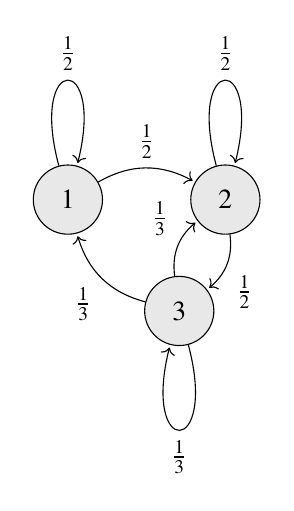
\begin{tikzpicture}[shorten >=1pt,node distance=2cm, scale =3, auto]
			\tikzstyle{every state}=[fill={rgb:black,1;white,10}]
			
			\node[state]   (q_1)                          {$1$};
			\node[state]   (q_2)  [right of=q_1]          {$2$};
			\node[state]   (q_3)  [below right of=q_1]          {$3$};
			
			\path[->]
			(q_1) edge [loop above] node {$\frac{1}{2}$}    (   )
			edge [bend left]  node {$\frac{1}{2}$}    (q_2)
			(q_2) edge [bend left]  node {$\frac{1}{2}$}    (q_3)
			edge [loop above] node {$\frac{1}{2}$}    ()
			(q_3) edge [bend left]  node {$\frac{1}{3}$}    (q_2)
			edge [bend left]  node {$\frac{1}{3}$}    (q_1)
			edge [loop below] node {$\frac{1}{3}$}    ();
		\end{tikzpicture}$
		
		\\  
		&\\
		&\\
		\hline
		\multirow{3}{*}{Checking whether the  } & \\
		& Here,\\chain is Irreducible
		& All the states are accessible to one another. \\and Aperiodic
		& $\implies$ They are in the same communication class. So, it is Irreducible.\\
		& \\
		& There exists the non- zero self-transition, which means that the chain \\
		& is Aperiodic.\\
		&\\ 
		& We know that if the Markov Chain is irreducible and aperiodic then \\
		& \qquad \qquad \qquad $\Vec{\pi}_{j} = \lim_{n \to \infty}P\{X_{n} = j\}$, $j = 1,...,N$ \\
		& These are the stationary probabilities. \\
		&\\
		\hline
		\multirow{3}{*}{Finding the Stationary} & \\
		& Stationary Probability can be represented as\\Probability Distributions
		& \qquad \qquad \qquad $\Vec{\pi} = \Vec{\pi} \vec{P}$\\
		& \\
		& \qquad $\implies$ $\myvec{v_{1}&&v_{2}&&v_{3}} = \myvec{v_{1}&&v_{2}&&v_{3}}\vec{P}$ \\
		& \\
		& Equating the above equation we get \\
		& \\
		& \qquad \qquad \qquad $\frac{1}{2}v_{1}-\frac{1}{3}v_{3} = 0$ $\label{eq:solutions/2018/dec/106/eq}$\\
		& \\
		& \qquad \qquad \qquad $\frac{1}{2}v_{1}-\frac{1}{2}v_{2} + \frac{1}{3}v_{3} = 0$\\
		& \\
		& \qquad \qquad \qquad $\frac{1}{2}v_{2}-\frac{2}{3}v_{3} = 0$\\
		& \\\
		& We see that summation of second and the third equation gives us the \\
		& first equation only. \\
		& And we know that the probability distribution will sum up to 1. \\
		& \\
		& \qquad \qquad \qquad $v_{1}+v_{2}+v_{3} = 1$ \\
		& \\
		& Therefore, we get the equation form as \\
		& \\
		& \qquad \qquad \qquad $\myvec{1&1&1\\\frac{1}{2}&0&\frac{-1}{3}\\\frac{1}{2}&\frac{-1}{2}&\frac{1}{3}}\myvec{v_{1}\\v_{2}\\v_{3}} = \myvec{1\\0\\0}$ \\
		& \\
		\hline
		\multirow{3}{*}{Solving the linear} & \\
		& The above linear equation can be solved using Gauss-Jordan method as\\equtions
		& \\
		& \qquad \qquad \qquad $\myvec{1&1&1&\vrule&1\\\frac{1}{2}&0&\frac{-1}{3}&\vrule&0\\\frac{1}{2}&\frac{-1}{2}&\frac{1}{3}&\vrule&0}$\\
		& \\
		& \qquad $\xleftrightarrow[]{R_2 \leftarrow R_2 - \frac{1}{2}R_1}$
		$\myvec{1&1&1&\vrule&1\\0&\frac{-1}{2}&\frac{-5}{6}&\vrule&\frac{-1}{2}\\\frac{1}{2}&\frac{-1}{2}&\frac{1}{3}&\vrule&0}$\\
		&\\
		& \qquad $\xleftrightarrow[]{R_3 \leftarrow R_3 - \frac{1}{2}R_1}$
		$\myvec{1&1&1&\vrule&1\\0&\frac{-1}{2}&\frac{-5}{6}&\vrule&\frac{-1}{2}\\0&-1&\frac{-1}{6}&\vrule&\frac{-1}{2}}$\\
		&\\
		& \qquad $\xleftrightarrow[]{R_2 \leftarrow \frac{-1}{2}R_2}$
		$\myvec{1&1&1&\vrule&1\\0&1&\frac{5}{3}&\vrule&1\\0&-1&\frac{-1}{6}&\vrule&\frac{-1}{2}}$\\
		&\\
		& \qquad $\xleftrightarrow[]{R_3 \leftarrow R_3 + R_2}$
		$\myvec{1&1&1&\vrule&1\\0&1&\frac{5}{3}&\vrule&1\\0&0&\frac{3}{2}&\vrule&\frac{1}{2}}$\\
		&\\
		& \qquad $\xleftrightarrow[]{R_3 \leftarrow \frac{3}{2}R_3}$
		$\myvec{1&1&1&\vrule&1\\0&1&\frac{5}{3}&\vrule&1\\0&0&1&\vrule&\frac{1}{3}}$\\
		&\\
		& \qquad $\xleftrightarrow[]{R_2 \leftarrow R_2 - \frac{5}{3}R_3}$
		$\myvec{1&1&1&\vrule&1\\0&1&0&\vrule&\frac{4}{9}\\0&0&1&\vrule&\frac{1}{3}}$\\
		&\\
		& \qquad $\xleftrightarrow[]{R_1 \leftarrow R_1 - R_3}$
		$\myvec{1&1&0&\vrule&\frac{2}{3}\\0&1&0&\vrule&\frac{4}{9}\\0&0&1&\vrule&\frac{1}{3}}$\\
		&\\
		& \qquad $\xleftrightarrow[]{R_1 \leftarrow R_1 - R_2}$
		$\myvec{1&0&0&\vrule&\frac{2}{9}\\0&1&0&\vrule&\frac{4}{9}\\0&0&1&\vrule&\frac{1}{3}}$\\
		&\\
		& $\therefore$, stationary probability distribution $\pi$ is given by \\
		& \qquad \qquad $\pi = \myvec{\frac{2}{9} & \frac{4}{9} & \frac{1}{3}}$ \\
		& \\
		\hline
		\multirow{3}{*}{Observations} & \\
		
		
		& Since the given transition probability matrix $\vec{P}$ is irreducible and aperiodic, \\
		& then $\lim_{n \to \infty} \vec{P}^{n}$ converges to a matrix with all rows identical and equal to $\vec{\pi}$. \\
		& \\
		& We were able to find $\vec{\pi}$ as $\myvec{\frac{2}{9} & \frac{4}{9} & \frac{1}{3}}$ \\
		& \\
		& $\lim_{n \to \infty} \vec{P}^{n} = \myvec{\frac{2}{9}&\frac{4}{9}&\frac{1}{3}\\\frac{2}{9}&\frac{4}{9}&\frac{1}{3}\\\frac{2}{9}&\frac{4}{9}&\frac{1}{3}}$\\
		& \\
		& From the above matrix, we get \\
		& \\
		& $\lim_{n \to \infty} \vec{P}^{n}_{11} = \frac{2}{9}$ \\
		&\\
		& $\lim_{n \to \infty} \vec{P}^{n}_{21} = \frac{2}{9}$ \\
		&\\
		& $\lim_{n \to \infty} \vec{P}^{n}_{32} = \frac{4}{9}$ \\
		&\\
		& $\lim_{n \to \infty} \vec{P}^{n}_{13} = \frac{1}{3}$ \\
		&\\
		\hline
		\multirow{3}{*}{Conclusion} & \\
		& From our observation we see that \\
		&\\
		& Options 1) and 4) are True.\\
		& \\
		\hline
\caption{}
\label{eq:solutions/2018/dec/106/table1}
	\end{longtable}
\twocolumn

\item Let $\vec{A}$ and $\vec{B}$ be real invertible matrices such that 
\begin{align}
    \vec{AB}=-\vec{BA}\label{eq:eq:solutions/2017/june/28/eq1}.
\end{align}
Then
\begin{enumerate}
    \item trace{$\vec{A}$} = trace($\vec{B}$) = 0
    \item trace{$\vec{A}$} = trace($\vec{B}$) = 1
    \item trace{$\vec{A}$} = 0, trace($\vec{B}$) = 1
    \item trace($\vec{A}$) = 1, trace($\vec{B}$) = 0
\end{enumerate}
%
\solution
See Tables \ref{eq:solutions/2018/dec/106/table0} and \ref{eq:solutions/2018/dec/106/table1}


\onecolumn
	\begin{longtable}{|l|l|}
		\hline
		\multirow{3}{*}{Irreducible Markov Chain} 
		& \\
		& A Markov chain is $\textbf{irreducible}$ if all the states communicate with each other,\\
		& i.e., if there is only one communication class.\\
		&\\
		\hline
		\multirow{3}{*}{Aperiodic Markov Chain} & \\
		& If there is a self-transition in the chain ($p^{ii}>0$ for some i), then the chain is\\
		& called as $\textbf{aperiodic}$\\
		& \\
		\hline
		\multirow{3}{*}{Stationary Distribution} & \\
		& A stationary distribution of a Markov chain is a probability distribution that\\
		& remains unchanged in the Markov chain as time progresses. Typically, it is\\
		& represented as a row vector $\Vec{\pi}$ whose entries are probabilities summing to 1,\\ 
		& and given transition matrix $\textbf{P}$, it satisfies\\
		& \\
		&  \qquad \qquad  \qquad$\Vec{\pi} = \Vec{\pi} \textbf{P}$\\
		& \\
		\hline
\caption{}
\label{eq:solutions/2018/dec/106/table0}
	\end{longtable}
	\begin{longtable}{|l|l|}
		\hline
		\multirow{3}{*}{Drawing Transition diagram} 
		& \\
		& 
		
		$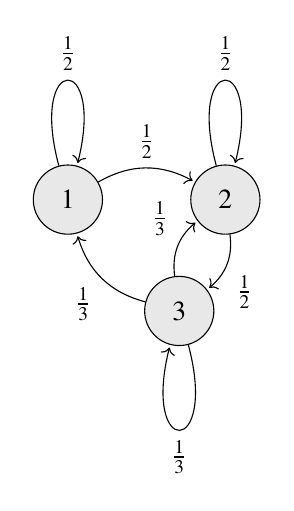
\begin{tikzpicture}[shorten >=1pt,node distance=2cm, scale =3, auto]
			\tikzstyle{every state}=[fill={rgb:black,1;white,10}]
			
			\node[state]   (q_1)                          {$1$};
			\node[state]   (q_2)  [right of=q_1]          {$2$};
			\node[state]   (q_3)  [below right of=q_1]          {$3$};
			
			\path[->]
			(q_1) edge [loop above] node {$\frac{1}{2}$}    (   )
			edge [bend left]  node {$\frac{1}{2}$}    (q_2)
			(q_2) edge [bend left]  node {$\frac{1}{2}$}    (q_3)
			edge [loop above] node {$\frac{1}{2}$}    ()
			(q_3) edge [bend left]  node {$\frac{1}{3}$}    (q_2)
			edge [bend left]  node {$\frac{1}{3}$}    (q_1)
			edge [loop below] node {$\frac{1}{3}$}    ();
		\end{tikzpicture}$
		
		\\  
		&\\
		&\\
		\hline
		\multirow{3}{*}{Checking whether the  } & \\
		& Here,\\chain is Irreducible
		& All the states are accessible to one another. \\and Aperiodic
		& $\implies$ They are in the same communication class. So, it is Irreducible.\\
		& \\
		& There exists the non- zero self-transition, which means that the chain \\
		& is Aperiodic.\\
		&\\ 
		& We know that if the Markov Chain is irreducible and aperiodic then \\
		& \qquad \qquad \qquad $\Vec{\pi}_{j} = \lim_{n \to \infty}P\{X_{n} = j\}$, $j = 1,...,N$ \\
		& These are the stationary probabilities. \\
		&\\
		\hline
		\multirow{3}{*}{Finding the Stationary} & \\
		& Stationary Probability can be represented as\\Probability Distributions
		& \qquad \qquad \qquad $\Vec{\pi} = \Vec{\pi} \vec{P}$\\
		& \\
		& \qquad $\implies$ $\myvec{v_{1}&&v_{2}&&v_{3}} = \myvec{v_{1}&&v_{2}&&v_{3}}\vec{P}$ \\
		& \\
		& Equating the above equation we get \\
		& \\
		& \qquad \qquad \qquad $\frac{1}{2}v_{1}-\frac{1}{3}v_{3} = 0$ $\label{eq:solutions/2018/dec/106/eq}$\\
		& \\
		& \qquad \qquad \qquad $\frac{1}{2}v_{1}-\frac{1}{2}v_{2} + \frac{1}{3}v_{3} = 0$\\
		& \\
		& \qquad \qquad \qquad $\frac{1}{2}v_{2}-\frac{2}{3}v_{3} = 0$\\
		& \\\
		& We see that summation of second and the third equation gives us the \\
		& first equation only. \\
		& And we know that the probability distribution will sum up to 1. \\
		& \\
		& \qquad \qquad \qquad $v_{1}+v_{2}+v_{3} = 1$ \\
		& \\
		& Therefore, we get the equation form as \\
		& \\
		& \qquad \qquad \qquad $\myvec{1&1&1\\\frac{1}{2}&0&\frac{-1}{3}\\\frac{1}{2}&\frac{-1}{2}&\frac{1}{3}}\myvec{v_{1}\\v_{2}\\v_{3}} = \myvec{1\\0\\0}$ \\
		& \\
		\hline
		\multirow{3}{*}{Solving the linear} & \\
		& The above linear equation can be solved using Gauss-Jordan method as\\equtions
		& \\
		& \qquad \qquad \qquad $\myvec{1&1&1&\vrule&1\\\frac{1}{2}&0&\frac{-1}{3}&\vrule&0\\\frac{1}{2}&\frac{-1}{2}&\frac{1}{3}&\vrule&0}$\\
		& \\
		& \qquad $\xleftrightarrow[]{R_2 \leftarrow R_2 - \frac{1}{2}R_1}$
		$\myvec{1&1&1&\vrule&1\\0&\frac{-1}{2}&\frac{-5}{6}&\vrule&\frac{-1}{2}\\\frac{1}{2}&\frac{-1}{2}&\frac{1}{3}&\vrule&0}$\\
		&\\
		& \qquad $\xleftrightarrow[]{R_3 \leftarrow R_3 - \frac{1}{2}R_1}$
		$\myvec{1&1&1&\vrule&1\\0&\frac{-1}{2}&\frac{-5}{6}&\vrule&\frac{-1}{2}\\0&-1&\frac{-1}{6}&\vrule&\frac{-1}{2}}$\\
		&\\
		& \qquad $\xleftrightarrow[]{R_2 \leftarrow \frac{-1}{2}R_2}$
		$\myvec{1&1&1&\vrule&1\\0&1&\frac{5}{3}&\vrule&1\\0&-1&\frac{-1}{6}&\vrule&\frac{-1}{2}}$\\
		&\\
		& \qquad $\xleftrightarrow[]{R_3 \leftarrow R_3 + R_2}$
		$\myvec{1&1&1&\vrule&1\\0&1&\frac{5}{3}&\vrule&1\\0&0&\frac{3}{2}&\vrule&\frac{1}{2}}$\\
		&\\
		& \qquad $\xleftrightarrow[]{R_3 \leftarrow \frac{3}{2}R_3}$
		$\myvec{1&1&1&\vrule&1\\0&1&\frac{5}{3}&\vrule&1\\0&0&1&\vrule&\frac{1}{3}}$\\
		&\\
		& \qquad $\xleftrightarrow[]{R_2 \leftarrow R_2 - \frac{5}{3}R_3}$
		$\myvec{1&1&1&\vrule&1\\0&1&0&\vrule&\frac{4}{9}\\0&0&1&\vrule&\frac{1}{3}}$\\
		&\\
		& \qquad $\xleftrightarrow[]{R_1 \leftarrow R_1 - R_3}$
		$\myvec{1&1&0&\vrule&\frac{2}{3}\\0&1&0&\vrule&\frac{4}{9}\\0&0&1&\vrule&\frac{1}{3}}$\\
		&\\
		& \qquad $\xleftrightarrow[]{R_1 \leftarrow R_1 - R_2}$
		$\myvec{1&0&0&\vrule&\frac{2}{9}\\0&1&0&\vrule&\frac{4}{9}\\0&0&1&\vrule&\frac{1}{3}}$\\
		&\\
		& $\therefore$, stationary probability distribution $\pi$ is given by \\
		& \qquad \qquad $\pi = \myvec{\frac{2}{9} & \frac{4}{9} & \frac{1}{3}}$ \\
		& \\
		\hline
		\multirow{3}{*}{Observations} & \\
		
		
		& Since the given transition probability matrix $\vec{P}$ is irreducible and aperiodic, \\
		& then $\lim_{n \to \infty} \vec{P}^{n}$ converges to a matrix with all rows identical and equal to $\vec{\pi}$. \\
		& \\
		& We were able to find $\vec{\pi}$ as $\myvec{\frac{2}{9} & \frac{4}{9} & \frac{1}{3}}$ \\
		& \\
		& $\lim_{n \to \infty} \vec{P}^{n} = \myvec{\frac{2}{9}&\frac{4}{9}&\frac{1}{3}\\\frac{2}{9}&\frac{4}{9}&\frac{1}{3}\\\frac{2}{9}&\frac{4}{9}&\frac{1}{3}}$\\
		& \\
		& From the above matrix, we get \\
		& \\
		& $\lim_{n \to \infty} \vec{P}^{n}_{11} = \frac{2}{9}$ \\
		&\\
		& $\lim_{n \to \infty} \vec{P}^{n}_{21} = \frac{2}{9}$ \\
		&\\
		& $\lim_{n \to \infty} \vec{P}^{n}_{32} = \frac{4}{9}$ \\
		&\\
		& $\lim_{n \to \infty} \vec{P}^{n}_{13} = \frac{1}{3}$ \\
		&\\
		\hline
		\multirow{3}{*}{Conclusion} & \\
		& From our observation we see that \\
		&\\
		& Options 1) and 4) are True.\\
		& \\
		\hline
\caption{}
\label{eq:solutions/2018/dec/106/table1}
	\end{longtable}
\twocolumn

\item Let $\vec{A}$ be an n $\times$ n self-adjoint matrix with eigenvalues $\lambda_1, \cdots, \lambda_2$.
Let,\begin{align} \norm{\vec{X}}_2=\sqrt{\vert\vec{X}_{1}^{2}\vert+\cdots+\vert\vec{X}_{n}^{2}\vert}\end{align} for $\vec{X}$=$(\vec{X}_{1},\cdots,\vec{X}_{n})\in \mathbb{C}^n$. If \begin{align}
p(\vec{A})=a_0\vec{I}+a_1\vec{A}+\cdots+a_n\vec{A}^n
\end{align}
then $sup_{\norm{\vec{X}}_{2}=1}\norm{p(\vec{A})\vec{X}}_2$ is equal to
%
\\
\solution
See Tables \ref{eq:solutions/2018/dec/106/table0} and \ref{eq:solutions/2018/dec/106/table1}


\onecolumn
	\begin{longtable}{|l|l|}
		\hline
		\multirow{3}{*}{Irreducible Markov Chain} 
		& \\
		& A Markov chain is $\textbf{irreducible}$ if all the states communicate with each other,\\
		& i.e., if there is only one communication class.\\
		&\\
		\hline
		\multirow{3}{*}{Aperiodic Markov Chain} & \\
		& If there is a self-transition in the chain ($p^{ii}>0$ for some i), then the chain is\\
		& called as $\textbf{aperiodic}$\\
		& \\
		\hline
		\multirow{3}{*}{Stationary Distribution} & \\
		& A stationary distribution of a Markov chain is a probability distribution that\\
		& remains unchanged in the Markov chain as time progresses. Typically, it is\\
		& represented as a row vector $\Vec{\pi}$ whose entries are probabilities summing to 1,\\ 
		& and given transition matrix $\textbf{P}$, it satisfies\\
		& \\
		&  \qquad \qquad  \qquad$\Vec{\pi} = \Vec{\pi} \textbf{P}$\\
		& \\
		\hline
\caption{}
\label{eq:solutions/2018/dec/106/table0}
	\end{longtable}
	\begin{longtable}{|l|l|}
		\hline
		\multirow{3}{*}{Drawing Transition diagram} 
		& \\
		& 
		
		$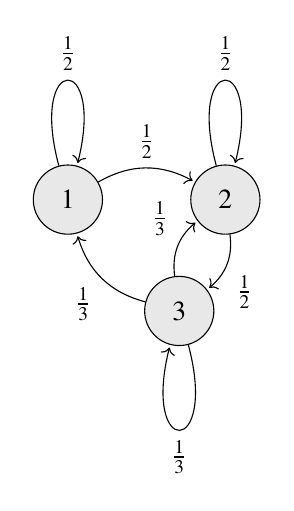
\begin{tikzpicture}[shorten >=1pt,node distance=2cm, scale =3, auto]
			\tikzstyle{every state}=[fill={rgb:black,1;white,10}]
			
			\node[state]   (q_1)                          {$1$};
			\node[state]   (q_2)  [right of=q_1]          {$2$};
			\node[state]   (q_3)  [below right of=q_1]          {$3$};
			
			\path[->]
			(q_1) edge [loop above] node {$\frac{1}{2}$}    (   )
			edge [bend left]  node {$\frac{1}{2}$}    (q_2)
			(q_2) edge [bend left]  node {$\frac{1}{2}$}    (q_3)
			edge [loop above] node {$\frac{1}{2}$}    ()
			(q_3) edge [bend left]  node {$\frac{1}{3}$}    (q_2)
			edge [bend left]  node {$\frac{1}{3}$}    (q_1)
			edge [loop below] node {$\frac{1}{3}$}    ();
		\end{tikzpicture}$
		
		\\  
		&\\
		&\\
		\hline
		\multirow{3}{*}{Checking whether the  } & \\
		& Here,\\chain is Irreducible
		& All the states are accessible to one another. \\and Aperiodic
		& $\implies$ They are in the same communication class. So, it is Irreducible.\\
		& \\
		& There exists the non- zero self-transition, which means that the chain \\
		& is Aperiodic.\\
		&\\ 
		& We know that if the Markov Chain is irreducible and aperiodic then \\
		& \qquad \qquad \qquad $\Vec{\pi}_{j} = \lim_{n \to \infty}P\{X_{n} = j\}$, $j = 1,...,N$ \\
		& These are the stationary probabilities. \\
		&\\
		\hline
		\multirow{3}{*}{Finding the Stationary} & \\
		& Stationary Probability can be represented as\\Probability Distributions
		& \qquad \qquad \qquad $\Vec{\pi} = \Vec{\pi} \vec{P}$\\
		& \\
		& \qquad $\implies$ $\myvec{v_{1}&&v_{2}&&v_{3}} = \myvec{v_{1}&&v_{2}&&v_{3}}\vec{P}$ \\
		& \\
		& Equating the above equation we get \\
		& \\
		& \qquad \qquad \qquad $\frac{1}{2}v_{1}-\frac{1}{3}v_{3} = 0$ $\label{eq:solutions/2018/dec/106/eq}$\\
		& \\
		& \qquad \qquad \qquad $\frac{1}{2}v_{1}-\frac{1}{2}v_{2} + \frac{1}{3}v_{3} = 0$\\
		& \\
		& \qquad \qquad \qquad $\frac{1}{2}v_{2}-\frac{2}{3}v_{3} = 0$\\
		& \\\
		& We see that summation of second and the third equation gives us the \\
		& first equation only. \\
		& And we know that the probability distribution will sum up to 1. \\
		& \\
		& \qquad \qquad \qquad $v_{1}+v_{2}+v_{3} = 1$ \\
		& \\
		& Therefore, we get the equation form as \\
		& \\
		& \qquad \qquad \qquad $\myvec{1&1&1\\\frac{1}{2}&0&\frac{-1}{3}\\\frac{1}{2}&\frac{-1}{2}&\frac{1}{3}}\myvec{v_{1}\\v_{2}\\v_{3}} = \myvec{1\\0\\0}$ \\
		& \\
		\hline
		\multirow{3}{*}{Solving the linear} & \\
		& The above linear equation can be solved using Gauss-Jordan method as\\equtions
		& \\
		& \qquad \qquad \qquad $\myvec{1&1&1&\vrule&1\\\frac{1}{2}&0&\frac{-1}{3}&\vrule&0\\\frac{1}{2}&\frac{-1}{2}&\frac{1}{3}&\vrule&0}$\\
		& \\
		& \qquad $\xleftrightarrow[]{R_2 \leftarrow R_2 - \frac{1}{2}R_1}$
		$\myvec{1&1&1&\vrule&1\\0&\frac{-1}{2}&\frac{-5}{6}&\vrule&\frac{-1}{2}\\\frac{1}{2}&\frac{-1}{2}&\frac{1}{3}&\vrule&0}$\\
		&\\
		& \qquad $\xleftrightarrow[]{R_3 \leftarrow R_3 - \frac{1}{2}R_1}$
		$\myvec{1&1&1&\vrule&1\\0&\frac{-1}{2}&\frac{-5}{6}&\vrule&\frac{-1}{2}\\0&-1&\frac{-1}{6}&\vrule&\frac{-1}{2}}$\\
		&\\
		& \qquad $\xleftrightarrow[]{R_2 \leftarrow \frac{-1}{2}R_2}$
		$\myvec{1&1&1&\vrule&1\\0&1&\frac{5}{3}&\vrule&1\\0&-1&\frac{-1}{6}&\vrule&\frac{-1}{2}}$\\
		&\\
		& \qquad $\xleftrightarrow[]{R_3 \leftarrow R_3 + R_2}$
		$\myvec{1&1&1&\vrule&1\\0&1&\frac{5}{3}&\vrule&1\\0&0&\frac{3}{2}&\vrule&\frac{1}{2}}$\\
		&\\
		& \qquad $\xleftrightarrow[]{R_3 \leftarrow \frac{3}{2}R_3}$
		$\myvec{1&1&1&\vrule&1\\0&1&\frac{5}{3}&\vrule&1\\0&0&1&\vrule&\frac{1}{3}}$\\
		&\\
		& \qquad $\xleftrightarrow[]{R_2 \leftarrow R_2 - \frac{5}{3}R_3}$
		$\myvec{1&1&1&\vrule&1\\0&1&0&\vrule&\frac{4}{9}\\0&0&1&\vrule&\frac{1}{3}}$\\
		&\\
		& \qquad $\xleftrightarrow[]{R_1 \leftarrow R_1 - R_3}$
		$\myvec{1&1&0&\vrule&\frac{2}{3}\\0&1&0&\vrule&\frac{4}{9}\\0&0&1&\vrule&\frac{1}{3}}$\\
		&\\
		& \qquad $\xleftrightarrow[]{R_1 \leftarrow R_1 - R_2}$
		$\myvec{1&0&0&\vrule&\frac{2}{9}\\0&1&0&\vrule&\frac{4}{9}\\0&0&1&\vrule&\frac{1}{3}}$\\
		&\\
		& $\therefore$, stationary probability distribution $\pi$ is given by \\
		& \qquad \qquad $\pi = \myvec{\frac{2}{9} & \frac{4}{9} & \frac{1}{3}}$ \\
		& \\
		\hline
		\multirow{3}{*}{Observations} & \\
		
		
		& Since the given transition probability matrix $\vec{P}$ is irreducible and aperiodic, \\
		& then $\lim_{n \to \infty} \vec{P}^{n}$ converges to a matrix with all rows identical and equal to $\vec{\pi}$. \\
		& \\
		& We were able to find $\vec{\pi}$ as $\myvec{\frac{2}{9} & \frac{4}{9} & \frac{1}{3}}$ \\
		& \\
		& $\lim_{n \to \infty} \vec{P}^{n} = \myvec{\frac{2}{9}&\frac{4}{9}&\frac{1}{3}\\\frac{2}{9}&\frac{4}{9}&\frac{1}{3}\\\frac{2}{9}&\frac{4}{9}&\frac{1}{3}}$\\
		& \\
		& From the above matrix, we get \\
		& \\
		& $\lim_{n \to \infty} \vec{P}^{n}_{11} = \frac{2}{9}$ \\
		&\\
		& $\lim_{n \to \infty} \vec{P}^{n}_{21} = \frac{2}{9}$ \\
		&\\
		& $\lim_{n \to \infty} \vec{P}^{n}_{32} = \frac{4}{9}$ \\
		&\\
		& $\lim_{n \to \infty} \vec{P}^{n}_{13} = \frac{1}{3}$ \\
		&\\
		\hline
		\multirow{3}{*}{Conclusion} & \\
		& From our observation we see that \\
		&\\
		& Options 1) and 4) are True.\\
		& \\
		\hline
\caption{}
\label{eq:solutions/2018/dec/106/table1}
	\end{longtable}
\twocolumn

\item Let $p \brak{x}= \alpha x^2+\beta x + \gamma$ be a polynomial, where $\alpha,\beta,\gamma \epsilon R$. Fix $X_0 \epsilon R$. Let $S=\{\brak{a,b,c}  \epsilon R^3: p \brak{x}= a \brak{x-x_0}^2+b \brak{x-x_0}+ c\}$ for all $x\epsilon R$. Find the number of elements in S is
\begin{enumerate}
    \item 0
    \item 1
    \item Strictly greater than 1 but finite
    \item Infinite
\end{enumerate}
%
\solution
See Tables \ref{eq:solutions/2018/dec/106/table0} and \ref{eq:solutions/2018/dec/106/table1}


\onecolumn
	\begin{longtable}{|l|l|}
		\hline
		\multirow{3}{*}{Irreducible Markov Chain} 
		& \\
		& A Markov chain is $\textbf{irreducible}$ if all the states communicate with each other,\\
		& i.e., if there is only one communication class.\\
		&\\
		\hline
		\multirow{3}{*}{Aperiodic Markov Chain} & \\
		& If there is a self-transition in the chain ($p^{ii}>0$ for some i), then the chain is\\
		& called as $\textbf{aperiodic}$\\
		& \\
		\hline
		\multirow{3}{*}{Stationary Distribution} & \\
		& A stationary distribution of a Markov chain is a probability distribution that\\
		& remains unchanged in the Markov chain as time progresses. Typically, it is\\
		& represented as a row vector $\Vec{\pi}$ whose entries are probabilities summing to 1,\\ 
		& and given transition matrix $\textbf{P}$, it satisfies\\
		& \\
		&  \qquad \qquad  \qquad$\Vec{\pi} = \Vec{\pi} \textbf{P}$\\
		& \\
		\hline
\caption{}
\label{eq:solutions/2018/dec/106/table0}
	\end{longtable}
	\begin{longtable}{|l|l|}
		\hline
		\multirow{3}{*}{Drawing Transition diagram} 
		& \\
		& 
		
		$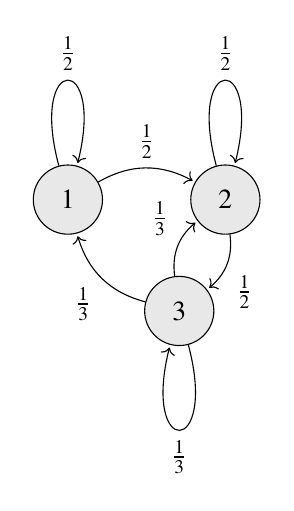
\begin{tikzpicture}[shorten >=1pt,node distance=2cm, scale =3, auto]
			\tikzstyle{every state}=[fill={rgb:black,1;white,10}]
			
			\node[state]   (q_1)                          {$1$};
			\node[state]   (q_2)  [right of=q_1]          {$2$};
			\node[state]   (q_3)  [below right of=q_1]          {$3$};
			
			\path[->]
			(q_1) edge [loop above] node {$\frac{1}{2}$}    (   )
			edge [bend left]  node {$\frac{1}{2}$}    (q_2)
			(q_2) edge [bend left]  node {$\frac{1}{2}$}    (q_3)
			edge [loop above] node {$\frac{1}{2}$}    ()
			(q_3) edge [bend left]  node {$\frac{1}{3}$}    (q_2)
			edge [bend left]  node {$\frac{1}{3}$}    (q_1)
			edge [loop below] node {$\frac{1}{3}$}    ();
		\end{tikzpicture}$
		
		\\  
		&\\
		&\\
		\hline
		\multirow{3}{*}{Checking whether the  } & \\
		& Here,\\chain is Irreducible
		& All the states are accessible to one another. \\and Aperiodic
		& $\implies$ They are in the same communication class. So, it is Irreducible.\\
		& \\
		& There exists the non- zero self-transition, which means that the chain \\
		& is Aperiodic.\\
		&\\ 
		& We know that if the Markov Chain is irreducible and aperiodic then \\
		& \qquad \qquad \qquad $\Vec{\pi}_{j} = \lim_{n \to \infty}P\{X_{n} = j\}$, $j = 1,...,N$ \\
		& These are the stationary probabilities. \\
		&\\
		\hline
		\multirow{3}{*}{Finding the Stationary} & \\
		& Stationary Probability can be represented as\\Probability Distributions
		& \qquad \qquad \qquad $\Vec{\pi} = \Vec{\pi} \vec{P}$\\
		& \\
		& \qquad $\implies$ $\myvec{v_{1}&&v_{2}&&v_{3}} = \myvec{v_{1}&&v_{2}&&v_{3}}\vec{P}$ \\
		& \\
		& Equating the above equation we get \\
		& \\
		& \qquad \qquad \qquad $\frac{1}{2}v_{1}-\frac{1}{3}v_{3} = 0$ $\label{eq:solutions/2018/dec/106/eq}$\\
		& \\
		& \qquad \qquad \qquad $\frac{1}{2}v_{1}-\frac{1}{2}v_{2} + \frac{1}{3}v_{3} = 0$\\
		& \\
		& \qquad \qquad \qquad $\frac{1}{2}v_{2}-\frac{2}{3}v_{3} = 0$\\
		& \\\
		& We see that summation of second and the third equation gives us the \\
		& first equation only. \\
		& And we know that the probability distribution will sum up to 1. \\
		& \\
		& \qquad \qquad \qquad $v_{1}+v_{2}+v_{3} = 1$ \\
		& \\
		& Therefore, we get the equation form as \\
		& \\
		& \qquad \qquad \qquad $\myvec{1&1&1\\\frac{1}{2}&0&\frac{-1}{3}\\\frac{1}{2}&\frac{-1}{2}&\frac{1}{3}}\myvec{v_{1}\\v_{2}\\v_{3}} = \myvec{1\\0\\0}$ \\
		& \\
		\hline
		\multirow{3}{*}{Solving the linear} & \\
		& The above linear equation can be solved using Gauss-Jordan method as\\equtions
		& \\
		& \qquad \qquad \qquad $\myvec{1&1&1&\vrule&1\\\frac{1}{2}&0&\frac{-1}{3}&\vrule&0\\\frac{1}{2}&\frac{-1}{2}&\frac{1}{3}&\vrule&0}$\\
		& \\
		& \qquad $\xleftrightarrow[]{R_2 \leftarrow R_2 - \frac{1}{2}R_1}$
		$\myvec{1&1&1&\vrule&1\\0&\frac{-1}{2}&\frac{-5}{6}&\vrule&\frac{-1}{2}\\\frac{1}{2}&\frac{-1}{2}&\frac{1}{3}&\vrule&0}$\\
		&\\
		& \qquad $\xleftrightarrow[]{R_3 \leftarrow R_3 - \frac{1}{2}R_1}$
		$\myvec{1&1&1&\vrule&1\\0&\frac{-1}{2}&\frac{-5}{6}&\vrule&\frac{-1}{2}\\0&-1&\frac{-1}{6}&\vrule&\frac{-1}{2}}$\\
		&\\
		& \qquad $\xleftrightarrow[]{R_2 \leftarrow \frac{-1}{2}R_2}$
		$\myvec{1&1&1&\vrule&1\\0&1&\frac{5}{3}&\vrule&1\\0&-1&\frac{-1}{6}&\vrule&\frac{-1}{2}}$\\
		&\\
		& \qquad $\xleftrightarrow[]{R_3 \leftarrow R_3 + R_2}$
		$\myvec{1&1&1&\vrule&1\\0&1&\frac{5}{3}&\vrule&1\\0&0&\frac{3}{2}&\vrule&\frac{1}{2}}$\\
		&\\
		& \qquad $\xleftrightarrow[]{R_3 \leftarrow \frac{3}{2}R_3}$
		$\myvec{1&1&1&\vrule&1\\0&1&\frac{5}{3}&\vrule&1\\0&0&1&\vrule&\frac{1}{3}}$\\
		&\\
		& \qquad $\xleftrightarrow[]{R_2 \leftarrow R_2 - \frac{5}{3}R_3}$
		$\myvec{1&1&1&\vrule&1\\0&1&0&\vrule&\frac{4}{9}\\0&0&1&\vrule&\frac{1}{3}}$\\
		&\\
		& \qquad $\xleftrightarrow[]{R_1 \leftarrow R_1 - R_3}$
		$\myvec{1&1&0&\vrule&\frac{2}{3}\\0&1&0&\vrule&\frac{4}{9}\\0&0&1&\vrule&\frac{1}{3}}$\\
		&\\
		& \qquad $\xleftrightarrow[]{R_1 \leftarrow R_1 - R_2}$
		$\myvec{1&0&0&\vrule&\frac{2}{9}\\0&1&0&\vrule&\frac{4}{9}\\0&0&1&\vrule&\frac{1}{3}}$\\
		&\\
		& $\therefore$, stationary probability distribution $\pi$ is given by \\
		& \qquad \qquad $\pi = \myvec{\frac{2}{9} & \frac{4}{9} & \frac{1}{3}}$ \\
		& \\
		\hline
		\multirow{3}{*}{Observations} & \\
		
		
		& Since the given transition probability matrix $\vec{P}$ is irreducible and aperiodic, \\
		& then $\lim_{n \to \infty} \vec{P}^{n}$ converges to a matrix with all rows identical and equal to $\vec{\pi}$. \\
		& \\
		& We were able to find $\vec{\pi}$ as $\myvec{\frac{2}{9} & \frac{4}{9} & \frac{1}{3}}$ \\
		& \\
		& $\lim_{n \to \infty} \vec{P}^{n} = \myvec{\frac{2}{9}&\frac{4}{9}&\frac{1}{3}\\\frac{2}{9}&\frac{4}{9}&\frac{1}{3}\\\frac{2}{9}&\frac{4}{9}&\frac{1}{3}}$\\
		& \\
		& From the above matrix, we get \\
		& \\
		& $\lim_{n \to \infty} \vec{P}^{n}_{11} = \frac{2}{9}$ \\
		&\\
		& $\lim_{n \to \infty} \vec{P}^{n}_{21} = \frac{2}{9}$ \\
		&\\
		& $\lim_{n \to \infty} \vec{P}^{n}_{32} = \frac{4}{9}$ \\
		&\\
		& $\lim_{n \to \infty} \vec{P}^{n}_{13} = \frac{1}{3}$ \\
		&\\
		\hline
		\multirow{3}{*}{Conclusion} & \\
		& From our observation we see that \\
		&\\
		& Options 1) and 4) are True.\\
		& \\
		\hline
\caption{}
\label{eq:solutions/2018/dec/106/table1}
	\end{longtable}
\twocolumn

\item Let
\begin{align}
\vec{A}=\myvec{1&0&2\\1&-2&0\\0&0&-3}
\end{align}
and $\vec{I}$ be the $3\times3$ identity matrix. If 
\begin{align}
6\vec{A}^{-1}=a\vec{A}^2+b\vec{A}+c\vec{I} \label{eq:solutions/2017/june/31/eq:1}
\end{align} for $a,b,c \in \mathbb{R}$ then (a,b,c) equals
\begin{enumerate}
\item (1,2,1)\\
\item (1,-1,2)\\
\item (4,1,1)\\
\item (1,4,1)
\end{enumerate}
\solution
See Tables \ref{eq:solutions/2018/dec/106/table0} and \ref{eq:solutions/2018/dec/106/table1}


\onecolumn
	\begin{longtable}{|l|l|}
		\hline
		\multirow{3}{*}{Irreducible Markov Chain} 
		& \\
		& A Markov chain is $\textbf{irreducible}$ if all the states communicate with each other,\\
		& i.e., if there is only one communication class.\\
		&\\
		\hline
		\multirow{3}{*}{Aperiodic Markov Chain} & \\
		& If there is a self-transition in the chain ($p^{ii}>0$ for some i), then the chain is\\
		& called as $\textbf{aperiodic}$\\
		& \\
		\hline
		\multirow{3}{*}{Stationary Distribution} & \\
		& A stationary distribution of a Markov chain is a probability distribution that\\
		& remains unchanged in the Markov chain as time progresses. Typically, it is\\
		& represented as a row vector $\Vec{\pi}$ whose entries are probabilities summing to 1,\\ 
		& and given transition matrix $\textbf{P}$, it satisfies\\
		& \\
		&  \qquad \qquad  \qquad$\Vec{\pi} = \Vec{\pi} \textbf{P}$\\
		& \\
		\hline
\caption{}
\label{eq:solutions/2018/dec/106/table0}
	\end{longtable}
	\begin{longtable}{|l|l|}
		\hline
		\multirow{3}{*}{Drawing Transition diagram} 
		& \\
		& 
		
		$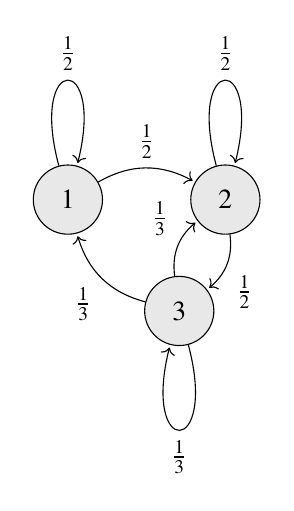
\begin{tikzpicture}[shorten >=1pt,node distance=2cm, scale =3, auto]
			\tikzstyle{every state}=[fill={rgb:black,1;white,10}]
			
			\node[state]   (q_1)                          {$1$};
			\node[state]   (q_2)  [right of=q_1]          {$2$};
			\node[state]   (q_3)  [below right of=q_1]          {$3$};
			
			\path[->]
			(q_1) edge [loop above] node {$\frac{1}{2}$}    (   )
			edge [bend left]  node {$\frac{1}{2}$}    (q_2)
			(q_2) edge [bend left]  node {$\frac{1}{2}$}    (q_3)
			edge [loop above] node {$\frac{1}{2}$}    ()
			(q_3) edge [bend left]  node {$\frac{1}{3}$}    (q_2)
			edge [bend left]  node {$\frac{1}{3}$}    (q_1)
			edge [loop below] node {$\frac{1}{3}$}    ();
		\end{tikzpicture}$
		
		\\  
		&\\
		&\\
		\hline
		\multirow{3}{*}{Checking whether the  } & \\
		& Here,\\chain is Irreducible
		& All the states are accessible to one another. \\and Aperiodic
		& $\implies$ They are in the same communication class. So, it is Irreducible.\\
		& \\
		& There exists the non- zero self-transition, which means that the chain \\
		& is Aperiodic.\\
		&\\ 
		& We know that if the Markov Chain is irreducible and aperiodic then \\
		& \qquad \qquad \qquad $\Vec{\pi}_{j} = \lim_{n \to \infty}P\{X_{n} = j\}$, $j = 1,...,N$ \\
		& These are the stationary probabilities. \\
		&\\
		\hline
		\multirow{3}{*}{Finding the Stationary} & \\
		& Stationary Probability can be represented as\\Probability Distributions
		& \qquad \qquad \qquad $\Vec{\pi} = \Vec{\pi} \vec{P}$\\
		& \\
		& \qquad $\implies$ $\myvec{v_{1}&&v_{2}&&v_{3}} = \myvec{v_{1}&&v_{2}&&v_{3}}\vec{P}$ \\
		& \\
		& Equating the above equation we get \\
		& \\
		& \qquad \qquad \qquad $\frac{1}{2}v_{1}-\frac{1}{3}v_{3} = 0$ $\label{eq:solutions/2018/dec/106/eq}$\\
		& \\
		& \qquad \qquad \qquad $\frac{1}{2}v_{1}-\frac{1}{2}v_{2} + \frac{1}{3}v_{3} = 0$\\
		& \\
		& \qquad \qquad \qquad $\frac{1}{2}v_{2}-\frac{2}{3}v_{3} = 0$\\
		& \\\
		& We see that summation of second and the third equation gives us the \\
		& first equation only. \\
		& And we know that the probability distribution will sum up to 1. \\
		& \\
		& \qquad \qquad \qquad $v_{1}+v_{2}+v_{3} = 1$ \\
		& \\
		& Therefore, we get the equation form as \\
		& \\
		& \qquad \qquad \qquad $\myvec{1&1&1\\\frac{1}{2}&0&\frac{-1}{3}\\\frac{1}{2}&\frac{-1}{2}&\frac{1}{3}}\myvec{v_{1}\\v_{2}\\v_{3}} = \myvec{1\\0\\0}$ \\
		& \\
		\hline
		\multirow{3}{*}{Solving the linear} & \\
		& The above linear equation can be solved using Gauss-Jordan method as\\equtions
		& \\
		& \qquad \qquad \qquad $\myvec{1&1&1&\vrule&1\\\frac{1}{2}&0&\frac{-1}{3}&\vrule&0\\\frac{1}{2}&\frac{-1}{2}&\frac{1}{3}&\vrule&0}$\\
		& \\
		& \qquad $\xleftrightarrow[]{R_2 \leftarrow R_2 - \frac{1}{2}R_1}$
		$\myvec{1&1&1&\vrule&1\\0&\frac{-1}{2}&\frac{-5}{6}&\vrule&\frac{-1}{2}\\\frac{1}{2}&\frac{-1}{2}&\frac{1}{3}&\vrule&0}$\\
		&\\
		& \qquad $\xleftrightarrow[]{R_3 \leftarrow R_3 - \frac{1}{2}R_1}$
		$\myvec{1&1&1&\vrule&1\\0&\frac{-1}{2}&\frac{-5}{6}&\vrule&\frac{-1}{2}\\0&-1&\frac{-1}{6}&\vrule&\frac{-1}{2}}$\\
		&\\
		& \qquad $\xleftrightarrow[]{R_2 \leftarrow \frac{-1}{2}R_2}$
		$\myvec{1&1&1&\vrule&1\\0&1&\frac{5}{3}&\vrule&1\\0&-1&\frac{-1}{6}&\vrule&\frac{-1}{2}}$\\
		&\\
		& \qquad $\xleftrightarrow[]{R_3 \leftarrow R_3 + R_2}$
		$\myvec{1&1&1&\vrule&1\\0&1&\frac{5}{3}&\vrule&1\\0&0&\frac{3}{2}&\vrule&\frac{1}{2}}$\\
		&\\
		& \qquad $\xleftrightarrow[]{R_3 \leftarrow \frac{3}{2}R_3}$
		$\myvec{1&1&1&\vrule&1\\0&1&\frac{5}{3}&\vrule&1\\0&0&1&\vrule&\frac{1}{3}}$\\
		&\\
		& \qquad $\xleftrightarrow[]{R_2 \leftarrow R_2 - \frac{5}{3}R_3}$
		$\myvec{1&1&1&\vrule&1\\0&1&0&\vrule&\frac{4}{9}\\0&0&1&\vrule&\frac{1}{3}}$\\
		&\\
		& \qquad $\xleftrightarrow[]{R_1 \leftarrow R_1 - R_3}$
		$\myvec{1&1&0&\vrule&\frac{2}{3}\\0&1&0&\vrule&\frac{4}{9}\\0&0&1&\vrule&\frac{1}{3}}$\\
		&\\
		& \qquad $\xleftrightarrow[]{R_1 \leftarrow R_1 - R_2}$
		$\myvec{1&0&0&\vrule&\frac{2}{9}\\0&1&0&\vrule&\frac{4}{9}\\0&0&1&\vrule&\frac{1}{3}}$\\
		&\\
		& $\therefore$, stationary probability distribution $\pi$ is given by \\
		& \qquad \qquad $\pi = \myvec{\frac{2}{9} & \frac{4}{9} & \frac{1}{3}}$ \\
		& \\
		\hline
		\multirow{3}{*}{Observations} & \\
		
		
		& Since the given transition probability matrix $\vec{P}$ is irreducible and aperiodic, \\
		& then $\lim_{n \to \infty} \vec{P}^{n}$ converges to a matrix with all rows identical and equal to $\vec{\pi}$. \\
		& \\
		& We were able to find $\vec{\pi}$ as $\myvec{\frac{2}{9} & \frac{4}{9} & \frac{1}{3}}$ \\
		& \\
		& $\lim_{n \to \infty} \vec{P}^{n} = \myvec{\frac{2}{9}&\frac{4}{9}&\frac{1}{3}\\\frac{2}{9}&\frac{4}{9}&\frac{1}{3}\\\frac{2}{9}&\frac{4}{9}&\frac{1}{3}}$\\
		& \\
		& From the above matrix, we get \\
		& \\
		& $\lim_{n \to \infty} \vec{P}^{n}_{11} = \frac{2}{9}$ \\
		&\\
		& $\lim_{n \to \infty} \vec{P}^{n}_{21} = \frac{2}{9}$ \\
		&\\
		& $\lim_{n \to \infty} \vec{P}^{n}_{32} = \frac{4}{9}$ \\
		&\\
		& $\lim_{n \to \infty} \vec{P}^{n}_{13} = \frac{1}{3}$ \\
		&\\
		\hline
		\multirow{3}{*}{Conclusion} & \\
		& From our observation we see that \\
		&\\
		& Options 1) and 4) are True.\\
		& \\
		\hline
\caption{}
\label{eq:solutions/2018/dec/106/table1}
	\end{longtable}
\twocolumn


%
\item Find the Eigenvalues of the matrix,
\begin{align}
\vec{A} = \myvec{1 & 1 & 2 \\ 1 & -2 & 5 \\ 2 & 5 & -3 }\label{eq:solutions/2017/june/32/eq:1}
\end{align}
\begin{enumerate}
\item -4, 3, -3
\item 4, 3, 1
\item 4, -4$\pm\sqrt{13}$
\item 4, -2$\pm\sqrt{7}$
\end{enumerate}
%
%
\solution
See Tables \ref{eq:solutions/2018/dec/106/table0} and \ref{eq:solutions/2018/dec/106/table1}


\onecolumn
	\begin{longtable}{|l|l|}
		\hline
		\multirow{3}{*}{Irreducible Markov Chain} 
		& \\
		& A Markov chain is $\textbf{irreducible}$ if all the states communicate with each other,\\
		& i.e., if there is only one communication class.\\
		&\\
		\hline
		\multirow{3}{*}{Aperiodic Markov Chain} & \\
		& If there is a self-transition in the chain ($p^{ii}>0$ for some i), then the chain is\\
		& called as $\textbf{aperiodic}$\\
		& \\
		\hline
		\multirow{3}{*}{Stationary Distribution} & \\
		& A stationary distribution of a Markov chain is a probability distribution that\\
		& remains unchanged in the Markov chain as time progresses. Typically, it is\\
		& represented as a row vector $\Vec{\pi}$ whose entries are probabilities summing to 1,\\ 
		& and given transition matrix $\textbf{P}$, it satisfies\\
		& \\
		&  \qquad \qquad  \qquad$\Vec{\pi} = \Vec{\pi} \textbf{P}$\\
		& \\
		\hline
\caption{}
\label{eq:solutions/2018/dec/106/table0}
	\end{longtable}
	\begin{longtable}{|l|l|}
		\hline
		\multirow{3}{*}{Drawing Transition diagram} 
		& \\
		& 
		
		$\begin{tikzpicture}[shorten >=1pt,node distance=2cm, scale =3, auto]
			\tikzstyle{every state}=[fill={rgb:black,1;white,10}]
			
			\node[state]   (q_1)                          {$1$};
			\node[state]   (q_2)  [right of=q_1]          {$2$};
			\node[state]   (q_3)  [below right of=q_1]          {$3$};
			
			\path[->]
			(q_1) edge [loop above] node {$\frac{1}{2}$}    (   )
			edge [bend left]  node {$\frac{1}{2}$}    (q_2)
			(q_2) edge [bend left]  node {$\frac{1}{2}$}    (q_3)
			edge [loop above] node {$\frac{1}{2}$}    ()
			(q_3) edge [bend left]  node {$\frac{1}{3}$}    (q_2)
			edge [bend left]  node {$\frac{1}{3}$}    (q_1)
			edge [loop below] node {$\frac{1}{3}$}    ();
		\end{tikzpicture}$
		
		\\  
		&\\
		&\\
		\hline
		\multirow{3}{*}{Checking whether the  } & \\
		& Here,\\chain is Irreducible
		& All the states are accessible to one another. \\and Aperiodic
		& $\implies$ They are in the same communication class. So, it is Irreducible.\\
		& \\
		& There exists the non- zero self-transition, which means that the chain \\
		& is Aperiodic.\\
		&\\ 
		& We know that if the Markov Chain is irreducible and aperiodic then \\
		& \qquad \qquad \qquad $\Vec{\pi}_{j} = \lim_{n \to \infty}P\{X_{n} = j\}$, $j = 1,...,N$ \\
		& These are the stationary probabilities. \\
		&\\
		\hline
		\multirow{3}{*}{Finding the Stationary} & \\
		& Stationary Probability can be represented as\\Probability Distributions
		& \qquad \qquad \qquad $\Vec{\pi} = \Vec{\pi} \vec{P}$\\
		& \\
		& \qquad $\implies$ $\myvec{v_{1}&&v_{2}&&v_{3}} = \myvec{v_{1}&&v_{2}&&v_{3}}\vec{P}$ \\
		& \\
		& Equating the above equation we get \\
		& \\
		& \qquad \qquad \qquad $\frac{1}{2}v_{1}-\frac{1}{3}v_{3} = 0$ $\label{eq:solutions/2018/dec/106/eq}$\\
		& \\
		& \qquad \qquad \qquad $\frac{1}{2}v_{1}-\frac{1}{2}v_{2} + \frac{1}{3}v_{3} = 0$\\
		& \\
		& \qquad \qquad \qquad $\frac{1}{2}v_{2}-\frac{2}{3}v_{3} = 0$\\
		& \\\
		& We see that summation of second and the third equation gives us the \\
		& first equation only. \\
		& And we know that the probability distribution will sum up to 1. \\
		& \\
		& \qquad \qquad \qquad $v_{1}+v_{2}+v_{3} = 1$ \\
		& \\
		& Therefore, we get the equation form as \\
		& \\
		& \qquad \qquad \qquad $\myvec{1&1&1\\\frac{1}{2}&0&\frac{-1}{3}\\\frac{1}{2}&\frac{-1}{2}&\frac{1}{3}}\myvec{v_{1}\\v_{2}\\v_{3}} = \myvec{1\\0\\0}$ \\
		& \\
		\hline
		\multirow{3}{*}{Solving the linear} & \\
		& The above linear equation can be solved using Gauss-Jordan method as\\equtions
		& \\
		& \qquad \qquad \qquad $\myvec{1&1&1&\vrule&1\\\frac{1}{2}&0&\frac{-1}{3}&\vrule&0\\\frac{1}{2}&\frac{-1}{2}&\frac{1}{3}&\vrule&0}$\\
		& \\
		& \qquad $\xleftrightarrow[]{R_2 \leftarrow R_2 - \frac{1}{2}R_1}$
		$\myvec{1&1&1&\vrule&1\\0&\frac{-1}{2}&\frac{-5}{6}&\vrule&\frac{-1}{2}\\\frac{1}{2}&\frac{-1}{2}&\frac{1}{3}&\vrule&0}$\\
		&\\
		& \qquad $\xleftrightarrow[]{R_3 \leftarrow R_3 - \frac{1}{2}R_1}$
		$\myvec{1&1&1&\vrule&1\\0&\frac{-1}{2}&\frac{-5}{6}&\vrule&\frac{-1}{2}\\0&-1&\frac{-1}{6}&\vrule&\frac{-1}{2}}$\\
		&\\
		& \qquad $\xleftrightarrow[]{R_2 \leftarrow \frac{-1}{2}R_2}$
		$\myvec{1&1&1&\vrule&1\\0&1&\frac{5}{3}&\vrule&1\\0&-1&\frac{-1}{6}&\vrule&\frac{-1}{2}}$\\
		&\\
		& \qquad $\xleftrightarrow[]{R_3 \leftarrow R_3 + R_2}$
		$\myvec{1&1&1&\vrule&1\\0&1&\frac{5}{3}&\vrule&1\\0&0&\frac{3}{2}&\vrule&\frac{1}{2}}$\\
		&\\
		& \qquad $\xleftrightarrow[]{R_3 \leftarrow \frac{3}{2}R_3}$
		$\myvec{1&1&1&\vrule&1\\0&1&\frac{5}{3}&\vrule&1\\0&0&1&\vrule&\frac{1}{3}}$\\
		&\\
		& \qquad $\xleftrightarrow[]{R_2 \leftarrow R_2 - \frac{5}{3}R_3}$
		$\myvec{1&1&1&\vrule&1\\0&1&0&\vrule&\frac{4}{9}\\0&0&1&\vrule&\frac{1}{3}}$\\
		&\\
		& \qquad $\xleftrightarrow[]{R_1 \leftarrow R_1 - R_3}$
		$\myvec{1&1&0&\vrule&\frac{2}{3}\\0&1&0&\vrule&\frac{4}{9}\\0&0&1&\vrule&\frac{1}{3}}$\\
		&\\
		& \qquad $\xleftrightarrow[]{R_1 \leftarrow R_1 - R_2}$
		$\myvec{1&0&0&\vrule&\frac{2}{9}\\0&1&0&\vrule&\frac{4}{9}\\0&0&1&\vrule&\frac{1}{3}}$\\
		&\\
		& $\therefore$, stationary probability distribution $\pi$ is given by \\
		& \qquad \qquad $\pi = \myvec{\frac{2}{9} & \frac{4}{9} & \frac{1}{3}}$ \\
		& \\
		\hline
		\multirow{3}{*}{Observations} & \\
		
		
		& Since the given transition probability matrix $\vec{P}$ is irreducible and aperiodic, \\
		& then $\lim_{n \to \infty} \vec{P}^{n}$ converges to a matrix with all rows identical and equal to $\vec{\pi}$. \\
		& \\
		& We were able to find $\vec{\pi}$ as $\myvec{\frac{2}{9} & \frac{4}{9} & \frac{1}{3}}$ \\
		& \\
		& $\lim_{n \to \infty} \vec{P}^{n} = \myvec{\frac{2}{9}&\frac{4}{9}&\frac{1}{3}\\\frac{2}{9}&\frac{4}{9}&\frac{1}{3}\\\frac{2}{9}&\frac{4}{9}&\frac{1}{3}}$\\
		& \\
		& From the above matrix, we get \\
		& \\
		& $\lim_{n \to \infty} \vec{P}^{n}_{11} = \frac{2}{9}$ \\
		&\\
		& $\lim_{n \to \infty} \vec{P}^{n}_{21} = \frac{2}{9}$ \\
		&\\
		& $\lim_{n \to \infty} \vec{P}^{n}_{32} = \frac{4}{9}$ \\
		&\\
		& $\lim_{n \to \infty} \vec{P}^{n}_{13} = \frac{1}{3}$ \\
		&\\
		\hline
		\multirow{3}{*}{Conclusion} & \\
		& From our observation we see that \\
		&\\
		& Options 1) and 4) are True.\\
		& \\
		\hline
\caption{}
\label{eq:solutions/2018/dec/106/table1}
	\end{longtable}
\twocolumn

\item Consider the vector space V of real polynomials of degree less than or equal to n. Fix distinct real numbers $a_0, a_1, \cdots, a_k$. For $p \in V$
\begin{align}
    max\cbrak{\abs{p(a_j)}: 0\leq j \leq k}
\end{align}
defines a norm on V
\begin{enumerate}
    \item only if $k<n$
    \item only if $k\ge n$
    \item if $ k+1\leq n$ 
    \item if $k \ge n+1$
\end{enumerate}
%
\solution
See Tables \ref{eq:solutions/2018/dec/106/table0} and \ref{eq:solutions/2018/dec/106/table1}


\onecolumn
	\begin{longtable}{|l|l|}
		\hline
		\multirow{3}{*}{Irreducible Markov Chain} 
		& \\
		& A Markov chain is $\textbf{irreducible}$ if all the states communicate with each other,\\
		& i.e., if there is only one communication class.\\
		&\\
		\hline
		\multirow{3}{*}{Aperiodic Markov Chain} & \\
		& If there is a self-transition in the chain ($p^{ii}>0$ for some i), then the chain is\\
		& called as $\textbf{aperiodic}$\\
		& \\
		\hline
		\multirow{3}{*}{Stationary Distribution} & \\
		& A stationary distribution of a Markov chain is a probability distribution that\\
		& remains unchanged in the Markov chain as time progresses. Typically, it is\\
		& represented as a row vector $\Vec{\pi}$ whose entries are probabilities summing to 1,\\ 
		& and given transition matrix $\textbf{P}$, it satisfies\\
		& \\
		&  \qquad \qquad  \qquad$\Vec{\pi} = \Vec{\pi} \textbf{P}$\\
		& \\
		\hline
\caption{}
\label{eq:solutions/2018/dec/106/table0}
	\end{longtable}
	\begin{longtable}{|l|l|}
		\hline
		\multirow{3}{*}{Drawing Transition diagram} 
		& \\
		& 
		
		$\begin{tikzpicture}[shorten >=1pt,node distance=2cm, scale =3, auto]
			\tikzstyle{every state}=[fill={rgb:black,1;white,10}]
			
			\node[state]   (q_1)                          {$1$};
			\node[state]   (q_2)  [right of=q_1]          {$2$};
			\node[state]   (q_3)  [below right of=q_1]          {$3$};
			
			\path[->]
			(q_1) edge [loop above] node {$\frac{1}{2}$}    (   )
			edge [bend left]  node {$\frac{1}{2}$}    (q_2)
			(q_2) edge [bend left]  node {$\frac{1}{2}$}    (q_3)
			edge [loop above] node {$\frac{1}{2}$}    ()
			(q_3) edge [bend left]  node {$\frac{1}{3}$}    (q_2)
			edge [bend left]  node {$\frac{1}{3}$}    (q_1)
			edge [loop below] node {$\frac{1}{3}$}    ();
		\end{tikzpicture}$
		
		\\  
		&\\
		&\\
		\hline
		\multirow{3}{*}{Checking whether the  } & \\
		& Here,\\chain is Irreducible
		& All the states are accessible to one another. \\and Aperiodic
		& $\implies$ They are in the same communication class. So, it is Irreducible.\\
		& \\
		& There exists the non- zero self-transition, which means that the chain \\
		& is Aperiodic.\\
		&\\ 
		& We know that if the Markov Chain is irreducible and aperiodic then \\
		& \qquad \qquad \qquad $\Vec{\pi}_{j} = \lim_{n \to \infty}P\{X_{n} = j\}$, $j = 1,...,N$ \\
		& These are the stationary probabilities. \\
		&\\
		\hline
		\multirow{3}{*}{Finding the Stationary} & \\
		& Stationary Probability can be represented as\\Probability Distributions
		& \qquad \qquad \qquad $\Vec{\pi} = \Vec{\pi} \vec{P}$\\
		& \\
		& \qquad $\implies$ $\myvec{v_{1}&&v_{2}&&v_{3}} = \myvec{v_{1}&&v_{2}&&v_{3}}\vec{P}$ \\
		& \\
		& Equating the above equation we get \\
		& \\
		& \qquad \qquad \qquad $\frac{1}{2}v_{1}-\frac{1}{3}v_{3} = 0$ $\label{eq:solutions/2018/dec/106/eq}$\\
		& \\
		& \qquad \qquad \qquad $\frac{1}{2}v_{1}-\frac{1}{2}v_{2} + \frac{1}{3}v_{3} = 0$\\
		& \\
		& \qquad \qquad \qquad $\frac{1}{2}v_{2}-\frac{2}{3}v_{3} = 0$\\
		& \\\
		& We see that summation of second and the third equation gives us the \\
		& first equation only. \\
		& And we know that the probability distribution will sum up to 1. \\
		& \\
		& \qquad \qquad \qquad $v_{1}+v_{2}+v_{3} = 1$ \\
		& \\
		& Therefore, we get the equation form as \\
		& \\
		& \qquad \qquad \qquad $\myvec{1&1&1\\\frac{1}{2}&0&\frac{-1}{3}\\\frac{1}{2}&\frac{-1}{2}&\frac{1}{3}}\myvec{v_{1}\\v_{2}\\v_{3}} = \myvec{1\\0\\0}$ \\
		& \\
		\hline
		\multirow{3}{*}{Solving the linear} & \\
		& The above linear equation can be solved using Gauss-Jordan method as\\equtions
		& \\
		& \qquad \qquad \qquad $\myvec{1&1&1&\vrule&1\\\frac{1}{2}&0&\frac{-1}{3}&\vrule&0\\\frac{1}{2}&\frac{-1}{2}&\frac{1}{3}&\vrule&0}$\\
		& \\
		& \qquad $\xleftrightarrow[]{R_2 \leftarrow R_2 - \frac{1}{2}R_1}$
		$\myvec{1&1&1&\vrule&1\\0&\frac{-1}{2}&\frac{-5}{6}&\vrule&\frac{-1}{2}\\\frac{1}{2}&\frac{-1}{2}&\frac{1}{3}&\vrule&0}$\\
		&\\
		& \qquad $\xleftrightarrow[]{R_3 \leftarrow R_3 - \frac{1}{2}R_1}$
		$\myvec{1&1&1&\vrule&1\\0&\frac{-1}{2}&\frac{-5}{6}&\vrule&\frac{-1}{2}\\0&-1&\frac{-1}{6}&\vrule&\frac{-1}{2}}$\\
		&\\
		& \qquad $\xleftrightarrow[]{R_2 \leftarrow \frac{-1}{2}R_2}$
		$\myvec{1&1&1&\vrule&1\\0&1&\frac{5}{3}&\vrule&1\\0&-1&\frac{-1}{6}&\vrule&\frac{-1}{2}}$\\
		&\\
		& \qquad $\xleftrightarrow[]{R_3 \leftarrow R_3 + R_2}$
		$\myvec{1&1&1&\vrule&1\\0&1&\frac{5}{3}&\vrule&1\\0&0&\frac{3}{2}&\vrule&\frac{1}{2}}$\\
		&\\
		& \qquad $\xleftrightarrow[]{R_3 \leftarrow \frac{3}{2}R_3}$
		$\myvec{1&1&1&\vrule&1\\0&1&\frac{5}{3}&\vrule&1\\0&0&1&\vrule&\frac{1}{3}}$\\
		&\\
		& \qquad $\xleftrightarrow[]{R_2 \leftarrow R_2 - \frac{5}{3}R_3}$
		$\myvec{1&1&1&\vrule&1\\0&1&0&\vrule&\frac{4}{9}\\0&0&1&\vrule&\frac{1}{3}}$\\
		&\\
		& \qquad $\xleftrightarrow[]{R_1 \leftarrow R_1 - R_3}$
		$\myvec{1&1&0&\vrule&\frac{2}{3}\\0&1&0&\vrule&\frac{4}{9}\\0&0&1&\vrule&\frac{1}{3}}$\\
		&\\
		& \qquad $\xleftrightarrow[]{R_1 \leftarrow R_1 - R_2}$
		$\myvec{1&0&0&\vrule&\frac{2}{9}\\0&1&0&\vrule&\frac{4}{9}\\0&0&1&\vrule&\frac{1}{3}}$\\
		&\\
		& $\therefore$, stationary probability distribution $\pi$ is given by \\
		& \qquad \qquad $\pi = \myvec{\frac{2}{9} & \frac{4}{9} & \frac{1}{3}}$ \\
		& \\
		\hline
		\multirow{3}{*}{Observations} & \\
		
		
		& Since the given transition probability matrix $\vec{P}$ is irreducible and aperiodic, \\
		& then $\lim_{n \to \infty} \vec{P}^{n}$ converges to a matrix with all rows identical and equal to $\vec{\pi}$. \\
		& \\
		& We were able to find $\vec{\pi}$ as $\myvec{\frac{2}{9} & \frac{4}{9} & \frac{1}{3}}$ \\
		& \\
		& $\lim_{n \to \infty} \vec{P}^{n} = \myvec{\frac{2}{9}&\frac{4}{9}&\frac{1}{3}\\\frac{2}{9}&\frac{4}{9}&\frac{1}{3}\\\frac{2}{9}&\frac{4}{9}&\frac{1}{3}}$\\
		& \\
		& From the above matrix, we get \\
		& \\
		& $\lim_{n \to \infty} \vec{P}^{n}_{11} = \frac{2}{9}$ \\
		&\\
		& $\lim_{n \to \infty} \vec{P}^{n}_{21} = \frac{2}{9}$ \\
		&\\
		& $\lim_{n \to \infty} \vec{P}^{n}_{32} = \frac{4}{9}$ \\
		&\\
		& $\lim_{n \to \infty} \vec{P}^{n}_{13} = \frac{1}{3}$ \\
		&\\
		\hline
		\multirow{3}{*}{Conclusion} & \\
		& From our observation we see that \\
		&\\
		& Options 1) and 4) are True.\\
		& \\
		\hline
\caption{}
\label{eq:solutions/2018/dec/106/table1}
	\end{longtable}
\twocolumn

\item Let \textbf{V} be the vector space of polynomials of degree at most 3 in a variable x with coefficients in $\mathbb{R}$. Let \textbf{T}=d/dx be the linear transformation of \textbf{V} to itself given by differentiation.\\

Which of the following are correct?\\
\begin{enumerate}
\item $\vec{T}$ is invertible
\item 0 is an eigenvalue of $\vec{T}$
\item There is a basis with respect to which the matrix of \textbf{T} is nilpotent.
\item The matrix of \textbf{T} with respect to the basis \myvec{1,1+x,1+x+x^2,1+x+x^2+x^3} is diagonal.
\end{enumerate}
\solution
See Tables \ref{eq:solutions/2018/dec/106/table0} and \ref{eq:solutions/2018/dec/106/table1}


\onecolumn
	\begin{longtable}{|l|l|}
		\hline
		\multirow{3}{*}{Irreducible Markov Chain} 
		& \\
		& A Markov chain is $\textbf{irreducible}$ if all the states communicate with each other,\\
		& i.e., if there is only one communication class.\\
		&\\
		\hline
		\multirow{3}{*}{Aperiodic Markov Chain} & \\
		& If there is a self-transition in the chain ($p^{ii}>0$ for some i), then the chain is\\
		& called as $\textbf{aperiodic}$\\
		& \\
		\hline
		\multirow{3}{*}{Stationary Distribution} & \\
		& A stationary distribution of a Markov chain is a probability distribution that\\
		& remains unchanged in the Markov chain as time progresses. Typically, it is\\
		& represented as a row vector $\Vec{\pi}$ whose entries are probabilities summing to 1,\\ 
		& and given transition matrix $\textbf{P}$, it satisfies\\
		& \\
		&  \qquad \qquad  \qquad$\Vec{\pi} = \Vec{\pi} \textbf{P}$\\
		& \\
		\hline
\caption{}
\label{eq:solutions/2018/dec/106/table0}
	\end{longtable}
	\begin{longtable}{|l|l|}
		\hline
		\multirow{3}{*}{Drawing Transition diagram} 
		& \\
		& 
		
		$\begin{tikzpicture}[shorten >=1pt,node distance=2cm, scale =3, auto]
			\tikzstyle{every state}=[fill={rgb:black,1;white,10}]
			
			\node[state]   (q_1)                          {$1$};
			\node[state]   (q_2)  [right of=q_1]          {$2$};
			\node[state]   (q_3)  [below right of=q_1]          {$3$};
			
			\path[->]
			(q_1) edge [loop above] node {$\frac{1}{2}$}    (   )
			edge [bend left]  node {$\frac{1}{2}$}    (q_2)
			(q_2) edge [bend left]  node {$\frac{1}{2}$}    (q_3)
			edge [loop above] node {$\frac{1}{2}$}    ()
			(q_3) edge [bend left]  node {$\frac{1}{3}$}    (q_2)
			edge [bend left]  node {$\frac{1}{3}$}    (q_1)
			edge [loop below] node {$\frac{1}{3}$}    ();
		\end{tikzpicture}$
		
		\\  
		&\\
		&\\
		\hline
		\multirow{3}{*}{Checking whether the  } & \\
		& Here,\\chain is Irreducible
		& All the states are accessible to one another. \\and Aperiodic
		& $\implies$ They are in the same communication class. So, it is Irreducible.\\
		& \\
		& There exists the non- zero self-transition, which means that the chain \\
		& is Aperiodic.\\
		&\\ 
		& We know that if the Markov Chain is irreducible and aperiodic then \\
		& \qquad \qquad \qquad $\Vec{\pi}_{j} = \lim_{n \to \infty}P\{X_{n} = j\}$, $j = 1,...,N$ \\
		& These are the stationary probabilities. \\
		&\\
		\hline
		\multirow{3}{*}{Finding the Stationary} & \\
		& Stationary Probability can be represented as\\Probability Distributions
		& \qquad \qquad \qquad $\Vec{\pi} = \Vec{\pi} \vec{P}$\\
		& \\
		& \qquad $\implies$ $\myvec{v_{1}&&v_{2}&&v_{3}} = \myvec{v_{1}&&v_{2}&&v_{3}}\vec{P}$ \\
		& \\
		& Equating the above equation we get \\
		& \\
		& \qquad \qquad \qquad $\frac{1}{2}v_{1}-\frac{1}{3}v_{3} = 0$ $\label{eq:solutions/2018/dec/106/eq}$\\
		& \\
		& \qquad \qquad \qquad $\frac{1}{2}v_{1}-\frac{1}{2}v_{2} + \frac{1}{3}v_{3} = 0$\\
		& \\
		& \qquad \qquad \qquad $\frac{1}{2}v_{2}-\frac{2}{3}v_{3} = 0$\\
		& \\\
		& We see that summation of second and the third equation gives us the \\
		& first equation only. \\
		& And we know that the probability distribution will sum up to 1. \\
		& \\
		& \qquad \qquad \qquad $v_{1}+v_{2}+v_{3} = 1$ \\
		& \\
		& Therefore, we get the equation form as \\
		& \\
		& \qquad \qquad \qquad $\myvec{1&1&1\\\frac{1}{2}&0&\frac{-1}{3}\\\frac{1}{2}&\frac{-1}{2}&\frac{1}{3}}\myvec{v_{1}\\v_{2}\\v_{3}} = \myvec{1\\0\\0}$ \\
		& \\
		\hline
		\multirow{3}{*}{Solving the linear} & \\
		& The above linear equation can be solved using Gauss-Jordan method as\\equtions
		& \\
		& \qquad \qquad \qquad $\myvec{1&1&1&\vrule&1\\\frac{1}{2}&0&\frac{-1}{3}&\vrule&0\\\frac{1}{2}&\frac{-1}{2}&\frac{1}{3}&\vrule&0}$\\
		& \\
		& \qquad $\xleftrightarrow[]{R_2 \leftarrow R_2 - \frac{1}{2}R_1}$
		$\myvec{1&1&1&\vrule&1\\0&\frac{-1}{2}&\frac{-5}{6}&\vrule&\frac{-1}{2}\\\frac{1}{2}&\frac{-1}{2}&\frac{1}{3}&\vrule&0}$\\
		&\\
		& \qquad $\xleftrightarrow[]{R_3 \leftarrow R_3 - \frac{1}{2}R_1}$
		$\myvec{1&1&1&\vrule&1\\0&\frac{-1}{2}&\frac{-5}{6}&\vrule&\frac{-1}{2}\\0&-1&\frac{-1}{6}&\vrule&\frac{-1}{2}}$\\
		&\\
		& \qquad $\xleftrightarrow[]{R_2 \leftarrow \frac{-1}{2}R_2}$
		$\myvec{1&1&1&\vrule&1\\0&1&\frac{5}{3}&\vrule&1\\0&-1&\frac{-1}{6}&\vrule&\frac{-1}{2}}$\\
		&\\
		& \qquad $\xleftrightarrow[]{R_3 \leftarrow R_3 + R_2}$
		$\myvec{1&1&1&\vrule&1\\0&1&\frac{5}{3}&\vrule&1\\0&0&\frac{3}{2}&\vrule&\frac{1}{2}}$\\
		&\\
		& \qquad $\xleftrightarrow[]{R_3 \leftarrow \frac{3}{2}R_3}$
		$\myvec{1&1&1&\vrule&1\\0&1&\frac{5}{3}&\vrule&1\\0&0&1&\vrule&\frac{1}{3}}$\\
		&\\
		& \qquad $\xleftrightarrow[]{R_2 \leftarrow R_2 - \frac{5}{3}R_3}$
		$\myvec{1&1&1&\vrule&1\\0&1&0&\vrule&\frac{4}{9}\\0&0&1&\vrule&\frac{1}{3}}$\\
		&\\
		& \qquad $\xleftrightarrow[]{R_1 \leftarrow R_1 - R_3}$
		$\myvec{1&1&0&\vrule&\frac{2}{3}\\0&1&0&\vrule&\frac{4}{9}\\0&0&1&\vrule&\frac{1}{3}}$\\
		&\\
		& \qquad $\xleftrightarrow[]{R_1 \leftarrow R_1 - R_2}$
		$\myvec{1&0&0&\vrule&\frac{2}{9}\\0&1&0&\vrule&\frac{4}{9}\\0&0&1&\vrule&\frac{1}{3}}$\\
		&\\
		& $\therefore$, stationary probability distribution $\pi$ is given by \\
		& \qquad \qquad $\pi = \myvec{\frac{2}{9} & \frac{4}{9} & \frac{1}{3}}$ \\
		& \\
		\hline
		\multirow{3}{*}{Observations} & \\
		
		
		& Since the given transition probability matrix $\vec{P}$ is irreducible and aperiodic, \\
		& then $\lim_{n \to \infty} \vec{P}^{n}$ converges to a matrix with all rows identical and equal to $\vec{\pi}$. \\
		& \\
		& We were able to find $\vec{\pi}$ as $\myvec{\frac{2}{9} & \frac{4}{9} & \frac{1}{3}}$ \\
		& \\
		& $\lim_{n \to \infty} \vec{P}^{n} = \myvec{\frac{2}{9}&\frac{4}{9}&\frac{1}{3}\\\frac{2}{9}&\frac{4}{9}&\frac{1}{3}\\\frac{2}{9}&\frac{4}{9}&\frac{1}{3}}$\\
		& \\
		& From the above matrix, we get \\
		& \\
		& $\lim_{n \to \infty} \vec{P}^{n}_{11} = \frac{2}{9}$ \\
		&\\
		& $\lim_{n \to \infty} \vec{P}^{n}_{21} = \frac{2}{9}$ \\
		&\\
		& $\lim_{n \to \infty} \vec{P}^{n}_{32} = \frac{4}{9}$ \\
		&\\
		& $\lim_{n \to \infty} \vec{P}^{n}_{13} = \frac{1}{3}$ \\
		&\\
		\hline
		\multirow{3}{*}{Conclusion} & \\
		& From our observation we see that \\
		&\\
		& Options 1) and 4) are True.\\
		& \\
		\hline
\caption{}
\label{eq:solutions/2018/dec/106/table1}
	\end{longtable}
\twocolumn

\item Let $m,n,r$ be natural numbers. Let $A$ be an $m\times n$ matrix with real entries such that $(AA^t)^r = I$, where $I$ is the $m \times m$ is identity matrix and $A^t$ is the transpose of the matrix $A$. We can conclude that\\
\begin{enumerate}
\item
$m = n$\\
\item
$AA^t$ is invertible\\
\item
$A^tA$ is invertible\\
\item
if $m=n$, then $A$ is invertible
\end{enumerate}
%
\solution
See Tables \ref{eq:solutions/2018/dec/106/table0} and \ref{eq:solutions/2018/dec/106/table1}


\onecolumn
	\begin{longtable}{|l|l|}
		\hline
		\multirow{3}{*}{Irreducible Markov Chain} 
		& \\
		& A Markov chain is $\textbf{irreducible}$ if all the states communicate with each other,\\
		& i.e., if there is only one communication class.\\
		&\\
		\hline
		\multirow{3}{*}{Aperiodic Markov Chain} & \\
		& If there is a self-transition in the chain ($p^{ii}>0$ for some i), then the chain is\\
		& called as $\textbf{aperiodic}$\\
		& \\
		\hline
		\multirow{3}{*}{Stationary Distribution} & \\
		& A stationary distribution of a Markov chain is a probability distribution that\\
		& remains unchanged in the Markov chain as time progresses. Typically, it is\\
		& represented as a row vector $\Vec{\pi}$ whose entries are probabilities summing to 1,\\ 
		& and given transition matrix $\textbf{P}$, it satisfies\\
		& \\
		&  \qquad \qquad  \qquad$\Vec{\pi} = \Vec{\pi} \textbf{P}$\\
		& \\
		\hline
\caption{}
\label{eq:solutions/2018/dec/106/table0}
	\end{longtable}
	\begin{longtable}{|l|l|}
		\hline
		\multirow{3}{*}{Drawing Transition diagram} 
		& \\
		& 
		
		$\begin{tikzpicture}[shorten >=1pt,node distance=2cm, scale =3, auto]
			\tikzstyle{every state}=[fill={rgb:black,1;white,10}]
			
			\node[state]   (q_1)                          {$1$};
			\node[state]   (q_2)  [right of=q_1]          {$2$};
			\node[state]   (q_3)  [below right of=q_1]          {$3$};
			
			\path[->]
			(q_1) edge [loop above] node {$\frac{1}{2}$}    (   )
			edge [bend left]  node {$\frac{1}{2}$}    (q_2)
			(q_2) edge [bend left]  node {$\frac{1}{2}$}    (q_3)
			edge [loop above] node {$\frac{1}{2}$}    ()
			(q_3) edge [bend left]  node {$\frac{1}{3}$}    (q_2)
			edge [bend left]  node {$\frac{1}{3}$}    (q_1)
			edge [loop below] node {$\frac{1}{3}$}    ();
		\end{tikzpicture}$
		
		\\  
		&\\
		&\\
		\hline
		\multirow{3}{*}{Checking whether the  } & \\
		& Here,\\chain is Irreducible
		& All the states are accessible to one another. \\and Aperiodic
		& $\implies$ They are in the same communication class. So, it is Irreducible.\\
		& \\
		& There exists the non- zero self-transition, which means that the chain \\
		& is Aperiodic.\\
		&\\ 
		& We know that if the Markov Chain is irreducible and aperiodic then \\
		& \qquad \qquad \qquad $\Vec{\pi}_{j} = \lim_{n \to \infty}P\{X_{n} = j\}$, $j = 1,...,N$ \\
		& These are the stationary probabilities. \\
		&\\
		\hline
		\multirow{3}{*}{Finding the Stationary} & \\
		& Stationary Probability can be represented as\\Probability Distributions
		& \qquad \qquad \qquad $\Vec{\pi} = \Vec{\pi} \vec{P}$\\
		& \\
		& \qquad $\implies$ $\myvec{v_{1}&&v_{2}&&v_{3}} = \myvec{v_{1}&&v_{2}&&v_{3}}\vec{P}$ \\
		& \\
		& Equating the above equation we get \\
		& \\
		& \qquad \qquad \qquad $\frac{1}{2}v_{1}-\frac{1}{3}v_{3} = 0$ $\label{eq:solutions/2018/dec/106/eq}$\\
		& \\
		& \qquad \qquad \qquad $\frac{1}{2}v_{1}-\frac{1}{2}v_{2} + \frac{1}{3}v_{3} = 0$\\
		& \\
		& \qquad \qquad \qquad $\frac{1}{2}v_{2}-\frac{2}{3}v_{3} = 0$\\
		& \\\
		& We see that summation of second and the third equation gives us the \\
		& first equation only. \\
		& And we know that the probability distribution will sum up to 1. \\
		& \\
		& \qquad \qquad \qquad $v_{1}+v_{2}+v_{3} = 1$ \\
		& \\
		& Therefore, we get the equation form as \\
		& \\
		& \qquad \qquad \qquad $\myvec{1&1&1\\\frac{1}{2}&0&\frac{-1}{3}\\\frac{1}{2}&\frac{-1}{2}&\frac{1}{3}}\myvec{v_{1}\\v_{2}\\v_{3}} = \myvec{1\\0\\0}$ \\
		& \\
		\hline
		\multirow{3}{*}{Solving the linear} & \\
		& The above linear equation can be solved using Gauss-Jordan method as\\equtions
		& \\
		& \qquad \qquad \qquad $\myvec{1&1&1&\vrule&1\\\frac{1}{2}&0&\frac{-1}{3}&\vrule&0\\\frac{1}{2}&\frac{-1}{2}&\frac{1}{3}&\vrule&0}$\\
		& \\
		& \qquad $\xleftrightarrow[]{R_2 \leftarrow R_2 - \frac{1}{2}R_1}$
		$\myvec{1&1&1&\vrule&1\\0&\frac{-1}{2}&\frac{-5}{6}&\vrule&\frac{-1}{2}\\\frac{1}{2}&\frac{-1}{2}&\frac{1}{3}&\vrule&0}$\\
		&\\
		& \qquad $\xleftrightarrow[]{R_3 \leftarrow R_3 - \frac{1}{2}R_1}$
		$\myvec{1&1&1&\vrule&1\\0&\frac{-1}{2}&\frac{-5}{6}&\vrule&\frac{-1}{2}\\0&-1&\frac{-1}{6}&\vrule&\frac{-1}{2}}$\\
		&\\
		& \qquad $\xleftrightarrow[]{R_2 \leftarrow \frac{-1}{2}R_2}$
		$\myvec{1&1&1&\vrule&1\\0&1&\frac{5}{3}&\vrule&1\\0&-1&\frac{-1}{6}&\vrule&\frac{-1}{2}}$\\
		&\\
		& \qquad $\xleftrightarrow[]{R_3 \leftarrow R_3 + R_2}$
		$\myvec{1&1&1&\vrule&1\\0&1&\frac{5}{3}&\vrule&1\\0&0&\frac{3}{2}&\vrule&\frac{1}{2}}$\\
		&\\
		& \qquad $\xleftrightarrow[]{R_3 \leftarrow \frac{3}{2}R_3}$
		$\myvec{1&1&1&\vrule&1\\0&1&\frac{5}{3}&\vrule&1\\0&0&1&\vrule&\frac{1}{3}}$\\
		&\\
		& \qquad $\xleftrightarrow[]{R_2 \leftarrow R_2 - \frac{5}{3}R_3}$
		$\myvec{1&1&1&\vrule&1\\0&1&0&\vrule&\frac{4}{9}\\0&0&1&\vrule&\frac{1}{3}}$\\
		&\\
		& \qquad $\xleftrightarrow[]{R_1 \leftarrow R_1 - R_3}$
		$\myvec{1&1&0&\vrule&\frac{2}{3}\\0&1&0&\vrule&\frac{4}{9}\\0&0&1&\vrule&\frac{1}{3}}$\\
		&\\
		& \qquad $\xleftrightarrow[]{R_1 \leftarrow R_1 - R_2}$
		$\myvec{1&0&0&\vrule&\frac{2}{9}\\0&1&0&\vrule&\frac{4}{9}\\0&0&1&\vrule&\frac{1}{3}}$\\
		&\\
		& $\therefore$, stationary probability distribution $\pi$ is given by \\
		& \qquad \qquad $\pi = \myvec{\frac{2}{9} & \frac{4}{9} & \frac{1}{3}}$ \\
		& \\
		\hline
		\multirow{3}{*}{Observations} & \\
		
		
		& Since the given transition probability matrix $\vec{P}$ is irreducible and aperiodic, \\
		& then $\lim_{n \to \infty} \vec{P}^{n}$ converges to a matrix with all rows identical and equal to $\vec{\pi}$. \\
		& \\
		& We were able to find $\vec{\pi}$ as $\myvec{\frac{2}{9} & \frac{4}{9} & \frac{1}{3}}$ \\
		& \\
		& $\lim_{n \to \infty} \vec{P}^{n} = \myvec{\frac{2}{9}&\frac{4}{9}&\frac{1}{3}\\\frac{2}{9}&\frac{4}{9}&\frac{1}{3}\\\frac{2}{9}&\frac{4}{9}&\frac{1}{3}}$\\
		& \\
		& From the above matrix, we get \\
		& \\
		& $\lim_{n \to \infty} \vec{P}^{n}_{11} = \frac{2}{9}$ \\
		&\\
		& $\lim_{n \to \infty} \vec{P}^{n}_{21} = \frac{2}{9}$ \\
		&\\
		& $\lim_{n \to \infty} \vec{P}^{n}_{32} = \frac{4}{9}$ \\
		&\\
		& $\lim_{n \to \infty} \vec{P}^{n}_{13} = \frac{1}{3}$ \\
		&\\
		\hline
		\multirow{3}{*}{Conclusion} & \\
		& From our observation we see that \\
		&\\
		& Options 1) and 4) are True.\\
		& \\
		\hline
\caption{}
\label{eq:solutions/2018/dec/106/table1}
	\end{longtable}
\twocolumn

\item Let $\vec{A}$ be a $n\times n$ real matrix with $\vec{A}^2=\vec{A}$. Then
\begin{enumerate}
	\item the eigenvalues of $\vec{A}$ are either 0 or 1
	\item $\vec{A}$ is a diagonal matrix with diagonal entries 0 or 1
	\item $rank(\vec{A})=trace(\vec{A})$
	\item if $rank(\vec{I-A})=trace(\vec{I-A})$
\end{enumerate}
%
%
\solution
See Tables \ref{eq:solutions/2018/dec/106/table0} and \ref{eq:solutions/2018/dec/106/table1}


\onecolumn
	\begin{longtable}{|l|l|}
		\hline
		\multirow{3}{*}{Irreducible Markov Chain} 
		& \\
		& A Markov chain is $\textbf{irreducible}$ if all the states communicate with each other,\\
		& i.e., if there is only one communication class.\\
		&\\
		\hline
		\multirow{3}{*}{Aperiodic Markov Chain} & \\
		& If there is a self-transition in the chain ($p^{ii}>0$ for some i), then the chain is\\
		& called as $\textbf{aperiodic}$\\
		& \\
		\hline
		\multirow{3}{*}{Stationary Distribution} & \\
		& A stationary distribution of a Markov chain is a probability distribution that\\
		& remains unchanged in the Markov chain as time progresses. Typically, it is\\
		& represented as a row vector $\Vec{\pi}$ whose entries are probabilities summing to 1,\\ 
		& and given transition matrix $\textbf{P}$, it satisfies\\
		& \\
		&  \qquad \qquad  \qquad$\Vec{\pi} = \Vec{\pi} \textbf{P}$\\
		& \\
		\hline
\caption{}
\label{eq:solutions/2018/dec/106/table0}
	\end{longtable}
	\begin{longtable}{|l|l|}
		\hline
		\multirow{3}{*}{Drawing Transition diagram} 
		& \\
		& 
		
		$\begin{tikzpicture}[shorten >=1pt,node distance=2cm, scale =3, auto]
			\tikzstyle{every state}=[fill={rgb:black,1;white,10}]
			
			\node[state]   (q_1)                          {$1$};
			\node[state]   (q_2)  [right of=q_1]          {$2$};
			\node[state]   (q_3)  [below right of=q_1]          {$3$};
			
			\path[->]
			(q_1) edge [loop above] node {$\frac{1}{2}$}    (   )
			edge [bend left]  node {$\frac{1}{2}$}    (q_2)
			(q_2) edge [bend left]  node {$\frac{1}{2}$}    (q_3)
			edge [loop above] node {$\frac{1}{2}$}    ()
			(q_3) edge [bend left]  node {$\frac{1}{3}$}    (q_2)
			edge [bend left]  node {$\frac{1}{3}$}    (q_1)
			edge [loop below] node {$\frac{1}{3}$}    ();
		\end{tikzpicture}$
		
		\\  
		&\\
		&\\
		\hline
		\multirow{3}{*}{Checking whether the  } & \\
		& Here,\\chain is Irreducible
		& All the states are accessible to one another. \\and Aperiodic
		& $\implies$ They are in the same communication class. So, it is Irreducible.\\
		& \\
		& There exists the non- zero self-transition, which means that the chain \\
		& is Aperiodic.\\
		&\\ 
		& We know that if the Markov Chain is irreducible and aperiodic then \\
		& \qquad \qquad \qquad $\Vec{\pi}_{j} = \lim_{n \to \infty}P\{X_{n} = j\}$, $j = 1,...,N$ \\
		& These are the stationary probabilities. \\
		&\\
		\hline
		\multirow{3}{*}{Finding the Stationary} & \\
		& Stationary Probability can be represented as\\Probability Distributions
		& \qquad \qquad \qquad $\Vec{\pi} = \Vec{\pi} \vec{P}$\\
		& \\
		& \qquad $\implies$ $\myvec{v_{1}&&v_{2}&&v_{3}} = \myvec{v_{1}&&v_{2}&&v_{3}}\vec{P}$ \\
		& \\
		& Equating the above equation we get \\
		& \\
		& \qquad \qquad \qquad $\frac{1}{2}v_{1}-\frac{1}{3}v_{3} = 0$ $\label{eq:solutions/2018/dec/106/eq}$\\
		& \\
		& \qquad \qquad \qquad $\frac{1}{2}v_{1}-\frac{1}{2}v_{2} + \frac{1}{3}v_{3} = 0$\\
		& \\
		& \qquad \qquad \qquad $\frac{1}{2}v_{2}-\frac{2}{3}v_{3} = 0$\\
		& \\\
		& We see that summation of second and the third equation gives us the \\
		& first equation only. \\
		& And we know that the probability distribution will sum up to 1. \\
		& \\
		& \qquad \qquad \qquad $v_{1}+v_{2}+v_{3} = 1$ \\
		& \\
		& Therefore, we get the equation form as \\
		& \\
		& \qquad \qquad \qquad $\myvec{1&1&1\\\frac{1}{2}&0&\frac{-1}{3}\\\frac{1}{2}&\frac{-1}{2}&\frac{1}{3}}\myvec{v_{1}\\v_{2}\\v_{3}} = \myvec{1\\0\\0}$ \\
		& \\
		\hline
		\multirow{3}{*}{Solving the linear} & \\
		& The above linear equation can be solved using Gauss-Jordan method as\\equtions
		& \\
		& \qquad \qquad \qquad $\myvec{1&1&1&\vrule&1\\\frac{1}{2}&0&\frac{-1}{3}&\vrule&0\\\frac{1}{2}&\frac{-1}{2}&\frac{1}{3}&\vrule&0}$\\
		& \\
		& \qquad $\xleftrightarrow[]{R_2 \leftarrow R_2 - \frac{1}{2}R_1}$
		$\myvec{1&1&1&\vrule&1\\0&\frac{-1}{2}&\frac{-5}{6}&\vrule&\frac{-1}{2}\\\frac{1}{2}&\frac{-1}{2}&\frac{1}{3}&\vrule&0}$\\
		&\\
		& \qquad $\xleftrightarrow[]{R_3 \leftarrow R_3 - \frac{1}{2}R_1}$
		$\myvec{1&1&1&\vrule&1\\0&\frac{-1}{2}&\frac{-5}{6}&\vrule&\frac{-1}{2}\\0&-1&\frac{-1}{6}&\vrule&\frac{-1}{2}}$\\
		&\\
		& \qquad $\xleftrightarrow[]{R_2 \leftarrow \frac{-1}{2}R_2}$
		$\myvec{1&1&1&\vrule&1\\0&1&\frac{5}{3}&\vrule&1\\0&-1&\frac{-1}{6}&\vrule&\frac{-1}{2}}$\\
		&\\
		& \qquad $\xleftrightarrow[]{R_3 \leftarrow R_3 + R_2}$
		$\myvec{1&1&1&\vrule&1\\0&1&\frac{5}{3}&\vrule&1\\0&0&\frac{3}{2}&\vrule&\frac{1}{2}}$\\
		&\\
		& \qquad $\xleftrightarrow[]{R_3 \leftarrow \frac{3}{2}R_3}$
		$\myvec{1&1&1&\vrule&1\\0&1&\frac{5}{3}&\vrule&1\\0&0&1&\vrule&\frac{1}{3}}$\\
		&\\
		& \qquad $\xleftrightarrow[]{R_2 \leftarrow R_2 - \frac{5}{3}R_3}$
		$\myvec{1&1&1&\vrule&1\\0&1&0&\vrule&\frac{4}{9}\\0&0&1&\vrule&\frac{1}{3}}$\\
		&\\
		& \qquad $\xleftrightarrow[]{R_1 \leftarrow R_1 - R_3}$
		$\myvec{1&1&0&\vrule&\frac{2}{3}\\0&1&0&\vrule&\frac{4}{9}\\0&0&1&\vrule&\frac{1}{3}}$\\
		&\\
		& \qquad $\xleftrightarrow[]{R_1 \leftarrow R_1 - R_2}$
		$\myvec{1&0&0&\vrule&\frac{2}{9}\\0&1&0&\vrule&\frac{4}{9}\\0&0&1&\vrule&\frac{1}{3}}$\\
		&\\
		& $\therefore$, stationary probability distribution $\pi$ is given by \\
		& \qquad \qquad $\pi = \myvec{\frac{2}{9} & \frac{4}{9} & \frac{1}{3}}$ \\
		& \\
		\hline
		\multirow{3}{*}{Observations} & \\
		
		
		& Since the given transition probability matrix $\vec{P}$ is irreducible and aperiodic, \\
		& then $\lim_{n \to \infty} \vec{P}^{n}$ converges to a matrix with all rows identical and equal to $\vec{\pi}$. \\
		& \\
		& We were able to find $\vec{\pi}$ as $\myvec{\frac{2}{9} & \frac{4}{9} & \frac{1}{3}}$ \\
		& \\
		& $\lim_{n \to \infty} \vec{P}^{n} = \myvec{\frac{2}{9}&\frac{4}{9}&\frac{1}{3}\\\frac{2}{9}&\frac{4}{9}&\frac{1}{3}\\\frac{2}{9}&\frac{4}{9}&\frac{1}{3}}$\\
		& \\
		& From the above matrix, we get \\
		& \\
		& $\lim_{n \to \infty} \vec{P}^{n}_{11} = \frac{2}{9}$ \\
		&\\
		& $\lim_{n \to \infty} \vec{P}^{n}_{21} = \frac{2}{9}$ \\
		&\\
		& $\lim_{n \to \infty} \vec{P}^{n}_{32} = \frac{4}{9}$ \\
		&\\
		& $\lim_{n \to \infty} \vec{P}^{n}_{13} = \frac{1}{3}$ \\
		&\\
		\hline
		\multirow{3}{*}{Conclusion} & \\
		& From our observation we see that \\
		&\\
		& Options 1) and 4) are True.\\
		& \\
		\hline
\caption{}
\label{eq:solutions/2018/dec/106/table1}
	\end{longtable}
\twocolumn

\item For any $n\times n$ matrix $B$, let $N(B)=\{X\in \mathbb{R}^n:BX=0\}$ be the null space of $B$. Let $A$ be a $4\times 4$ matrix with $dim(N(A-4I))=2, dim(N(A-2I))=1$ and $rank(A)=3$
Which of the following are true?
\begin{enumerate}
\item 0,2 and 4 are eigenvalues of A
\item determinant(A)=0
\item A is not diagonalizable
\item trace(A)=8
\end{enumerate}
%
\solution
See Tables \ref{eq:solutions/2018/dec/106/table0} and \ref{eq:solutions/2018/dec/106/table1}


\onecolumn
	\begin{longtable}{|l|l|}
		\hline
		\multirow{3}{*}{Irreducible Markov Chain} 
		& \\
		& A Markov chain is $\textbf{irreducible}$ if all the states communicate with each other,\\
		& i.e., if there is only one communication class.\\
		&\\
		\hline
		\multirow{3}{*}{Aperiodic Markov Chain} & \\
		& If there is a self-transition in the chain ($p^{ii}>0$ for some i), then the chain is\\
		& called as $\textbf{aperiodic}$\\
		& \\
		\hline
		\multirow{3}{*}{Stationary Distribution} & \\
		& A stationary distribution of a Markov chain is a probability distribution that\\
		& remains unchanged in the Markov chain as time progresses. Typically, it is\\
		& represented as a row vector $\Vec{\pi}$ whose entries are probabilities summing to 1,\\ 
		& and given transition matrix $\textbf{P}$, it satisfies\\
		& \\
		&  \qquad \qquad  \qquad$\Vec{\pi} = \Vec{\pi} \textbf{P}$\\
		& \\
		\hline
\caption{}
\label{eq:solutions/2018/dec/106/table0}
	\end{longtable}
	\begin{longtable}{|l|l|}
		\hline
		\multirow{3}{*}{Drawing Transition diagram} 
		& \\
		& 
		
		$\begin{tikzpicture}[shorten >=1pt,node distance=2cm, scale =3, auto]
			\tikzstyle{every state}=[fill={rgb:black,1;white,10}]
			
			\node[state]   (q_1)                          {$1$};
			\node[state]   (q_2)  [right of=q_1]          {$2$};
			\node[state]   (q_3)  [below right of=q_1]          {$3$};
			
			\path[->]
			(q_1) edge [loop above] node {$\frac{1}{2}$}    (   )
			edge [bend left]  node {$\frac{1}{2}$}    (q_2)
			(q_2) edge [bend left]  node {$\frac{1}{2}$}    (q_3)
			edge [loop above] node {$\frac{1}{2}$}    ()
			(q_3) edge [bend left]  node {$\frac{1}{3}$}    (q_2)
			edge [bend left]  node {$\frac{1}{3}$}    (q_1)
			edge [loop below] node {$\frac{1}{3}$}    ();
		\end{tikzpicture}$
		
		\\  
		&\\
		&\\
		\hline
		\multirow{3}{*}{Checking whether the  } & \\
		& Here,\\chain is Irreducible
		& All the states are accessible to one another. \\and Aperiodic
		& $\implies$ They are in the same communication class. So, it is Irreducible.\\
		& \\
		& There exists the non- zero self-transition, which means that the chain \\
		& is Aperiodic.\\
		&\\ 
		& We know that if the Markov Chain is irreducible and aperiodic then \\
		& \qquad \qquad \qquad $\Vec{\pi}_{j} = \lim_{n \to \infty}P\{X_{n} = j\}$, $j = 1,...,N$ \\
		& These are the stationary probabilities. \\
		&\\
		\hline
		\multirow{3}{*}{Finding the Stationary} & \\
		& Stationary Probability can be represented as\\Probability Distributions
		& \qquad \qquad \qquad $\Vec{\pi} = \Vec{\pi} \vec{P}$\\
		& \\
		& \qquad $\implies$ $\myvec{v_{1}&&v_{2}&&v_{3}} = \myvec{v_{1}&&v_{2}&&v_{3}}\vec{P}$ \\
		& \\
		& Equating the above equation we get \\
		& \\
		& \qquad \qquad \qquad $\frac{1}{2}v_{1}-\frac{1}{3}v_{3} = 0$ $\label{eq:solutions/2018/dec/106/eq}$\\
		& \\
		& \qquad \qquad \qquad $\frac{1}{2}v_{1}-\frac{1}{2}v_{2} + \frac{1}{3}v_{3} = 0$\\
		& \\
		& \qquad \qquad \qquad $\frac{1}{2}v_{2}-\frac{2}{3}v_{3} = 0$\\
		& \\\
		& We see that summation of second and the third equation gives us the \\
		& first equation only. \\
		& And we know that the probability distribution will sum up to 1. \\
		& \\
		& \qquad \qquad \qquad $v_{1}+v_{2}+v_{3} = 1$ \\
		& \\
		& Therefore, we get the equation form as \\
		& \\
		& \qquad \qquad \qquad $\myvec{1&1&1\\\frac{1}{2}&0&\frac{-1}{3}\\\frac{1}{2}&\frac{-1}{2}&\frac{1}{3}}\myvec{v_{1}\\v_{2}\\v_{3}} = \myvec{1\\0\\0}$ \\
		& \\
		\hline
		\multirow{3}{*}{Solving the linear} & \\
		& The above linear equation can be solved using Gauss-Jordan method as\\equtions
		& \\
		& \qquad \qquad \qquad $\myvec{1&1&1&\vrule&1\\\frac{1}{2}&0&\frac{-1}{3}&\vrule&0\\\frac{1}{2}&\frac{-1}{2}&\frac{1}{3}&\vrule&0}$\\
		& \\
		& \qquad $\xleftrightarrow[]{R_2 \leftarrow R_2 - \frac{1}{2}R_1}$
		$\myvec{1&1&1&\vrule&1\\0&\frac{-1}{2}&\frac{-5}{6}&\vrule&\frac{-1}{2}\\\frac{1}{2}&\frac{-1}{2}&\frac{1}{3}&\vrule&0}$\\
		&\\
		& \qquad $\xleftrightarrow[]{R_3 \leftarrow R_3 - \frac{1}{2}R_1}$
		$\myvec{1&1&1&\vrule&1\\0&\frac{-1}{2}&\frac{-5}{6}&\vrule&\frac{-1}{2}\\0&-1&\frac{-1}{6}&\vrule&\frac{-1}{2}}$\\
		&\\
		& \qquad $\xleftrightarrow[]{R_2 \leftarrow \frac{-1}{2}R_2}$
		$\myvec{1&1&1&\vrule&1\\0&1&\frac{5}{3}&\vrule&1\\0&-1&\frac{-1}{6}&\vrule&\frac{-1}{2}}$\\
		&\\
		& \qquad $\xleftrightarrow[]{R_3 \leftarrow R_3 + R_2}$
		$\myvec{1&1&1&\vrule&1\\0&1&\frac{5}{3}&\vrule&1\\0&0&\frac{3}{2}&\vrule&\frac{1}{2}}$\\
		&\\
		& \qquad $\xleftrightarrow[]{R_3 \leftarrow \frac{3}{2}R_3}$
		$\myvec{1&1&1&\vrule&1\\0&1&\frac{5}{3}&\vrule&1\\0&0&1&\vrule&\frac{1}{3}}$\\
		&\\
		& \qquad $\xleftrightarrow[]{R_2 \leftarrow R_2 - \frac{5}{3}R_3}$
		$\myvec{1&1&1&\vrule&1\\0&1&0&\vrule&\frac{4}{9}\\0&0&1&\vrule&\frac{1}{3}}$\\
		&\\
		& \qquad $\xleftrightarrow[]{R_1 \leftarrow R_1 - R_3}$
		$\myvec{1&1&0&\vrule&\frac{2}{3}\\0&1&0&\vrule&\frac{4}{9}\\0&0&1&\vrule&\frac{1}{3}}$\\
		&\\
		& \qquad $\xleftrightarrow[]{R_1 \leftarrow R_1 - R_2}$
		$\myvec{1&0&0&\vrule&\frac{2}{9}\\0&1&0&\vrule&\frac{4}{9}\\0&0&1&\vrule&\frac{1}{3}}$\\
		&\\
		& $\therefore$, stationary probability distribution $\pi$ is given by \\
		& \qquad \qquad $\pi = \myvec{\frac{2}{9} & \frac{4}{9} & \frac{1}{3}}$ \\
		& \\
		\hline
		\multirow{3}{*}{Observations} & \\
		
		
		& Since the given transition probability matrix $\vec{P}$ is irreducible and aperiodic, \\
		& then $\lim_{n \to \infty} \vec{P}^{n}$ converges to a matrix with all rows identical and equal to $\vec{\pi}$. \\
		& \\
		& We were able to find $\vec{\pi}$ as $\myvec{\frac{2}{9} & \frac{4}{9} & \frac{1}{3}}$ \\
		& \\
		& $\lim_{n \to \infty} \vec{P}^{n} = \myvec{\frac{2}{9}&\frac{4}{9}&\frac{1}{3}\\\frac{2}{9}&\frac{4}{9}&\frac{1}{3}\\\frac{2}{9}&\frac{4}{9}&\frac{1}{3}}$\\
		& \\
		& From the above matrix, we get \\
		& \\
		& $\lim_{n \to \infty} \vec{P}^{n}_{11} = \frac{2}{9}$ \\
		&\\
		& $\lim_{n \to \infty} \vec{P}^{n}_{21} = \frac{2}{9}$ \\
		&\\
		& $\lim_{n \to \infty} \vec{P}^{n}_{32} = \frac{4}{9}$ \\
		&\\
		& $\lim_{n \to \infty} \vec{P}^{n}_{13} = \frac{1}{3}$ \\
		&\\
		\hline
		\multirow{3}{*}{Conclusion} & \\
		& From our observation we see that \\
		&\\
		& Options 1) and 4) are True.\\
		& \\
		\hline
\caption{}
\label{eq:solutions/2018/dec/106/table1}
	\end{longtable}
\twocolumn

\item Which of the following 3x3 matrices are diagonizable over $\mathbb{R}?$\\
\begin{enumerate}
    \item \myvec{1&2&3\\0&4&5\\0&0&6}
    \item \myvec{0&1&0\\-1&0&0\\0&0&1}
    \item \myvec{1&2&3\\2&1&4\\3&4&1}
    \item \myvec{0&1&2\\0&0&1\\0&0&0}
\end{enumerate}
%
\solution
See Tables \ref{eq:solutions/2018/dec/106/table0} and \ref{eq:solutions/2018/dec/106/table1}


\onecolumn
	\begin{longtable}{|l|l|}
		\hline
		\multirow{3}{*}{Irreducible Markov Chain} 
		& \\
		& A Markov chain is $\textbf{irreducible}$ if all the states communicate with each other,\\
		& i.e., if there is only one communication class.\\
		&\\
		\hline
		\multirow{3}{*}{Aperiodic Markov Chain} & \\
		& If there is a self-transition in the chain ($p^{ii}>0$ for some i), then the chain is\\
		& called as $\textbf{aperiodic}$\\
		& \\
		\hline
		\multirow{3}{*}{Stationary Distribution} & \\
		& A stationary distribution of a Markov chain is a probability distribution that\\
		& remains unchanged in the Markov chain as time progresses. Typically, it is\\
		& represented as a row vector $\Vec{\pi}$ whose entries are probabilities summing to 1,\\ 
		& and given transition matrix $\textbf{P}$, it satisfies\\
		& \\
		&  \qquad \qquad  \qquad$\Vec{\pi} = \Vec{\pi} \textbf{P}$\\
		& \\
		\hline
\caption{}
\label{eq:solutions/2018/dec/106/table0}
	\end{longtable}
	\begin{longtable}{|l|l|}
		\hline
		\multirow{3}{*}{Drawing Transition diagram} 
		& \\
		& 
		
		$\begin{tikzpicture}[shorten >=1pt,node distance=2cm, scale =3, auto]
			\tikzstyle{every state}=[fill={rgb:black,1;white,10}]
			
			\node[state]   (q_1)                          {$1$};
			\node[state]   (q_2)  [right of=q_1]          {$2$};
			\node[state]   (q_3)  [below right of=q_1]          {$3$};
			
			\path[->]
			(q_1) edge [loop above] node {$\frac{1}{2}$}    (   )
			edge [bend left]  node {$\frac{1}{2}$}    (q_2)
			(q_2) edge [bend left]  node {$\frac{1}{2}$}    (q_3)
			edge [loop above] node {$\frac{1}{2}$}    ()
			(q_3) edge [bend left]  node {$\frac{1}{3}$}    (q_2)
			edge [bend left]  node {$\frac{1}{3}$}    (q_1)
			edge [loop below] node {$\frac{1}{3}$}    ();
		\end{tikzpicture}$
		
		\\  
		&\\
		&\\
		\hline
		\multirow{3}{*}{Checking whether the  } & \\
		& Here,\\chain is Irreducible
		& All the states are accessible to one another. \\and Aperiodic
		& $\implies$ They are in the same communication class. So, it is Irreducible.\\
		& \\
		& There exists the non- zero self-transition, which means that the chain \\
		& is Aperiodic.\\
		&\\ 
		& We know that if the Markov Chain is irreducible and aperiodic then \\
		& \qquad \qquad \qquad $\Vec{\pi}_{j} = \lim_{n \to \infty}P\{X_{n} = j\}$, $j = 1,...,N$ \\
		& These are the stationary probabilities. \\
		&\\
		\hline
		\multirow{3}{*}{Finding the Stationary} & \\
		& Stationary Probability can be represented as\\Probability Distributions
		& \qquad \qquad \qquad $\Vec{\pi} = \Vec{\pi} \vec{P}$\\
		& \\
		& \qquad $\implies$ $\myvec{v_{1}&&v_{2}&&v_{3}} = \myvec{v_{1}&&v_{2}&&v_{3}}\vec{P}$ \\
		& \\
		& Equating the above equation we get \\
		& \\
		& \qquad \qquad \qquad $\frac{1}{2}v_{1}-\frac{1}{3}v_{3} = 0$ $\label{eq:solutions/2018/dec/106/eq}$\\
		& \\
		& \qquad \qquad \qquad $\frac{1}{2}v_{1}-\frac{1}{2}v_{2} + \frac{1}{3}v_{3} = 0$\\
		& \\
		& \qquad \qquad \qquad $\frac{1}{2}v_{2}-\frac{2}{3}v_{3} = 0$\\
		& \\\
		& We see that summation of second and the third equation gives us the \\
		& first equation only. \\
		& And we know that the probability distribution will sum up to 1. \\
		& \\
		& \qquad \qquad \qquad $v_{1}+v_{2}+v_{3} = 1$ \\
		& \\
		& Therefore, we get the equation form as \\
		& \\
		& \qquad \qquad \qquad $\myvec{1&1&1\\\frac{1}{2}&0&\frac{-1}{3}\\\frac{1}{2}&\frac{-1}{2}&\frac{1}{3}}\myvec{v_{1}\\v_{2}\\v_{3}} = \myvec{1\\0\\0}$ \\
		& \\
		\hline
		\multirow{3}{*}{Solving the linear} & \\
		& The above linear equation can be solved using Gauss-Jordan method as\\equtions
		& \\
		& \qquad \qquad \qquad $\myvec{1&1&1&\vrule&1\\\frac{1}{2}&0&\frac{-1}{3}&\vrule&0\\\frac{1}{2}&\frac{-1}{2}&\frac{1}{3}&\vrule&0}$\\
		& \\
		& \qquad $\xleftrightarrow[]{R_2 \leftarrow R_2 - \frac{1}{2}R_1}$
		$\myvec{1&1&1&\vrule&1\\0&\frac{-1}{2}&\frac{-5}{6}&\vrule&\frac{-1}{2}\\\frac{1}{2}&\frac{-1}{2}&\frac{1}{3}&\vrule&0}$\\
		&\\
		& \qquad $\xleftrightarrow[]{R_3 \leftarrow R_3 - \frac{1}{2}R_1}$
		$\myvec{1&1&1&\vrule&1\\0&\frac{-1}{2}&\frac{-5}{6}&\vrule&\frac{-1}{2}\\0&-1&\frac{-1}{6}&\vrule&\frac{-1}{2}}$\\
		&\\
		& \qquad $\xleftrightarrow[]{R_2 \leftarrow \frac{-1}{2}R_2}$
		$\myvec{1&1&1&\vrule&1\\0&1&\frac{5}{3}&\vrule&1\\0&-1&\frac{-1}{6}&\vrule&\frac{-1}{2}}$\\
		&\\
		& \qquad $\xleftrightarrow[]{R_3 \leftarrow R_3 + R_2}$
		$\myvec{1&1&1&\vrule&1\\0&1&\frac{5}{3}&\vrule&1\\0&0&\frac{3}{2}&\vrule&\frac{1}{2}}$\\
		&\\
		& \qquad $\xleftrightarrow[]{R_3 \leftarrow \frac{3}{2}R_3}$
		$\myvec{1&1&1&\vrule&1\\0&1&\frac{5}{3}&\vrule&1\\0&0&1&\vrule&\frac{1}{3}}$\\
		&\\
		& \qquad $\xleftrightarrow[]{R_2 \leftarrow R_2 - \frac{5}{3}R_3}$
		$\myvec{1&1&1&\vrule&1\\0&1&0&\vrule&\frac{4}{9}\\0&0&1&\vrule&\frac{1}{3}}$\\
		&\\
		& \qquad $\xleftrightarrow[]{R_1 \leftarrow R_1 - R_3}$
		$\myvec{1&1&0&\vrule&\frac{2}{3}\\0&1&0&\vrule&\frac{4}{9}\\0&0&1&\vrule&\frac{1}{3}}$\\
		&\\
		& \qquad $\xleftrightarrow[]{R_1 \leftarrow R_1 - R_2}$
		$\myvec{1&0&0&\vrule&\frac{2}{9}\\0&1&0&\vrule&\frac{4}{9}\\0&0&1&\vrule&\frac{1}{3}}$\\
		&\\
		& $\therefore$, stationary probability distribution $\pi$ is given by \\
		& \qquad \qquad $\pi = \myvec{\frac{2}{9} & \frac{4}{9} & \frac{1}{3}}$ \\
		& \\
		\hline
		\multirow{3}{*}{Observations} & \\
		
		
		& Since the given transition probability matrix $\vec{P}$ is irreducible and aperiodic, \\
		& then $\lim_{n \to \infty} \vec{P}^{n}$ converges to a matrix with all rows identical and equal to $\vec{\pi}$. \\
		& \\
		& We were able to find $\vec{\pi}$ as $\myvec{\frac{2}{9} & \frac{4}{9} & \frac{1}{3}}$ \\
		& \\
		& $\lim_{n \to \infty} \vec{P}^{n} = \myvec{\frac{2}{9}&\frac{4}{9}&\frac{1}{3}\\\frac{2}{9}&\frac{4}{9}&\frac{1}{3}\\\frac{2}{9}&\frac{4}{9}&\frac{1}{3}}$\\
		& \\
		& From the above matrix, we get \\
		& \\
		& $\lim_{n \to \infty} \vec{P}^{n}_{11} = \frac{2}{9}$ \\
		&\\
		& $\lim_{n \to \infty} \vec{P}^{n}_{21} = \frac{2}{9}$ \\
		&\\
		& $\lim_{n \to \infty} \vec{P}^{n}_{32} = \frac{4}{9}$ \\
		&\\
		& $\lim_{n \to \infty} \vec{P}^{n}_{13} = \frac{1}{3}$ \\
		&\\
		\hline
		\multirow{3}{*}{Conclusion} & \\
		& From our observation we see that \\
		&\\
		& Options 1) and 4) are True.\\
		& \\
		\hline
\caption{}
\label{eq:solutions/2018/dec/106/table1}
	\end{longtable}
\twocolumn

\twocolumn
\item Let $\vec{A} = \myvec{3 & 1 & 2 \\ 1 & 2 & 3 \\ 2 & 3 & 1  }$ and $\vec{Q(X) = X^TAX}$ for $\vec{X} \in \mathbb{R}^{3}$. Then
\begin{enumerate}
	\item $\vec{A}$ has exactly two positive eigen values.
	\item all the eigen values of $\vec{A}$ are positive.
	\item $\vec{Q(X)} \geq 0 $ $\forall$ $\vec{X}$ $\in$ $\mathbb{R}^3$
	\item $\vec{Q(X)} < 0 $ for some $\vec{X}$ $\in$ $\mathbb{R}^3$
\end{enumerate}
%
%
\solution
See Tables \ref{eq:solutions/2018/dec/106/table0} and \ref{eq:solutions/2018/dec/106/table1}


\onecolumn
	\begin{longtable}{|l|l|}
		\hline
		\multirow{3}{*}{Irreducible Markov Chain} 
		& \\
		& A Markov chain is $\textbf{irreducible}$ if all the states communicate with each other,\\
		& i.e., if there is only one communication class.\\
		&\\
		\hline
		\multirow{3}{*}{Aperiodic Markov Chain} & \\
		& If there is a self-transition in the chain ($p^{ii}>0$ for some i), then the chain is\\
		& called as $\textbf{aperiodic}$\\
		& \\
		\hline
		\multirow{3}{*}{Stationary Distribution} & \\
		& A stationary distribution of a Markov chain is a probability distribution that\\
		& remains unchanged in the Markov chain as time progresses. Typically, it is\\
		& represented as a row vector $\Vec{\pi}$ whose entries are probabilities summing to 1,\\ 
		& and given transition matrix $\textbf{P}$, it satisfies\\
		& \\
		&  \qquad \qquad  \qquad$\Vec{\pi} = \Vec{\pi} \textbf{P}$\\
		& \\
		\hline
\caption{}
\label{eq:solutions/2018/dec/106/table0}
	\end{longtable}
	\begin{longtable}{|l|l|}
		\hline
		\multirow{3}{*}{Drawing Transition diagram} 
		& \\
		& 
		
		$\begin{tikzpicture}[shorten >=1pt,node distance=2cm, scale =3, auto]
			\tikzstyle{every state}=[fill={rgb:black,1;white,10}]
			
			\node[state]   (q_1)                          {$1$};
			\node[state]   (q_2)  [right of=q_1]          {$2$};
			\node[state]   (q_3)  [below right of=q_1]          {$3$};
			
			\path[->]
			(q_1) edge [loop above] node {$\frac{1}{2}$}    (   )
			edge [bend left]  node {$\frac{1}{2}$}    (q_2)
			(q_2) edge [bend left]  node {$\frac{1}{2}$}    (q_3)
			edge [loop above] node {$\frac{1}{2}$}    ()
			(q_3) edge [bend left]  node {$\frac{1}{3}$}    (q_2)
			edge [bend left]  node {$\frac{1}{3}$}    (q_1)
			edge [loop below] node {$\frac{1}{3}$}    ();
		\end{tikzpicture}$
		
		\\  
		&\\
		&\\
		\hline
		\multirow{3}{*}{Checking whether the  } & \\
		& Here,\\chain is Irreducible
		& All the states are accessible to one another. \\and Aperiodic
		& $\implies$ They are in the same communication class. So, it is Irreducible.\\
		& \\
		& There exists the non- zero self-transition, which means that the chain \\
		& is Aperiodic.\\
		&\\ 
		& We know that if the Markov Chain is irreducible and aperiodic then \\
		& \qquad \qquad \qquad $\Vec{\pi}_{j} = \lim_{n \to \infty}P\{X_{n} = j\}$, $j = 1,...,N$ \\
		& These are the stationary probabilities. \\
		&\\
		\hline
		\multirow{3}{*}{Finding the Stationary} & \\
		& Stationary Probability can be represented as\\Probability Distributions
		& \qquad \qquad \qquad $\Vec{\pi} = \Vec{\pi} \vec{P}$\\
		& \\
		& \qquad $\implies$ $\myvec{v_{1}&&v_{2}&&v_{3}} = \myvec{v_{1}&&v_{2}&&v_{3}}\vec{P}$ \\
		& \\
		& Equating the above equation we get \\
		& \\
		& \qquad \qquad \qquad $\frac{1}{2}v_{1}-\frac{1}{3}v_{3} = 0$ $\label{eq:solutions/2018/dec/106/eq}$\\
		& \\
		& \qquad \qquad \qquad $\frac{1}{2}v_{1}-\frac{1}{2}v_{2} + \frac{1}{3}v_{3} = 0$\\
		& \\
		& \qquad \qquad \qquad $\frac{1}{2}v_{2}-\frac{2}{3}v_{3} = 0$\\
		& \\\
		& We see that summation of second and the third equation gives us the \\
		& first equation only. \\
		& And we know that the probability distribution will sum up to 1. \\
		& \\
		& \qquad \qquad \qquad $v_{1}+v_{2}+v_{3} = 1$ \\
		& \\
		& Therefore, we get the equation form as \\
		& \\
		& \qquad \qquad \qquad $\myvec{1&1&1\\\frac{1}{2}&0&\frac{-1}{3}\\\frac{1}{2}&\frac{-1}{2}&\frac{1}{3}}\myvec{v_{1}\\v_{2}\\v_{3}} = \myvec{1\\0\\0}$ \\
		& \\
		\hline
		\multirow{3}{*}{Solving the linear} & \\
		& The above linear equation can be solved using Gauss-Jordan method as\\equtions
		& \\
		& \qquad \qquad \qquad $\myvec{1&1&1&\vrule&1\\\frac{1}{2}&0&\frac{-1}{3}&\vrule&0\\\frac{1}{2}&\frac{-1}{2}&\frac{1}{3}&\vrule&0}$\\
		& \\
		& \qquad $\xleftrightarrow[]{R_2 \leftarrow R_2 - \frac{1}{2}R_1}$
		$\myvec{1&1&1&\vrule&1\\0&\frac{-1}{2}&\frac{-5}{6}&\vrule&\frac{-1}{2}\\\frac{1}{2}&\frac{-1}{2}&\frac{1}{3}&\vrule&0}$\\
		&\\
		& \qquad $\xleftrightarrow[]{R_3 \leftarrow R_3 - \frac{1}{2}R_1}$
		$\myvec{1&1&1&\vrule&1\\0&\frac{-1}{2}&\frac{-5}{6}&\vrule&\frac{-1}{2}\\0&-1&\frac{-1}{6}&\vrule&\frac{-1}{2}}$\\
		&\\
		& \qquad $\xleftrightarrow[]{R_2 \leftarrow \frac{-1}{2}R_2}$
		$\myvec{1&1&1&\vrule&1\\0&1&\frac{5}{3}&\vrule&1\\0&-1&\frac{-1}{6}&\vrule&\frac{-1}{2}}$\\
		&\\
		& \qquad $\xleftrightarrow[]{R_3 \leftarrow R_3 + R_2}$
		$\myvec{1&1&1&\vrule&1\\0&1&\frac{5}{3}&\vrule&1\\0&0&\frac{3}{2}&\vrule&\frac{1}{2}}$\\
		&\\
		& \qquad $\xleftrightarrow[]{R_3 \leftarrow \frac{3}{2}R_3}$
		$\myvec{1&1&1&\vrule&1\\0&1&\frac{5}{3}&\vrule&1\\0&0&1&\vrule&\frac{1}{3}}$\\
		&\\
		& \qquad $\xleftrightarrow[]{R_2 \leftarrow R_2 - \frac{5}{3}R_3}$
		$\myvec{1&1&1&\vrule&1\\0&1&0&\vrule&\frac{4}{9}\\0&0&1&\vrule&\frac{1}{3}}$\\
		&\\
		& \qquad $\xleftrightarrow[]{R_1 \leftarrow R_1 - R_3}$
		$\myvec{1&1&0&\vrule&\frac{2}{3}\\0&1&0&\vrule&\frac{4}{9}\\0&0&1&\vrule&\frac{1}{3}}$\\
		&\\
		& \qquad $\xleftrightarrow[]{R_1 \leftarrow R_1 - R_2}$
		$\myvec{1&0&0&\vrule&\frac{2}{9}\\0&1&0&\vrule&\frac{4}{9}\\0&0&1&\vrule&\frac{1}{3}}$\\
		&\\
		& $\therefore$, stationary probability distribution $\pi$ is given by \\
		& \qquad \qquad $\pi = \myvec{\frac{2}{9} & \frac{4}{9} & \frac{1}{3}}$ \\
		& \\
		\hline
		\multirow{3}{*}{Observations} & \\
		
		
		& Since the given transition probability matrix $\vec{P}$ is irreducible and aperiodic, \\
		& then $\lim_{n \to \infty} \vec{P}^{n}$ converges to a matrix with all rows identical and equal to $\vec{\pi}$. \\
		& \\
		& We were able to find $\vec{\pi}$ as $\myvec{\frac{2}{9} & \frac{4}{9} & \frac{1}{3}}$ \\
		& \\
		& $\lim_{n \to \infty} \vec{P}^{n} = \myvec{\frac{2}{9}&\frac{4}{9}&\frac{1}{3}\\\frac{2}{9}&\frac{4}{9}&\frac{1}{3}\\\frac{2}{9}&\frac{4}{9}&\frac{1}{3}}$\\
		& \\
		& From the above matrix, we get \\
		& \\
		& $\lim_{n \to \infty} \vec{P}^{n}_{11} = \frac{2}{9}$ \\
		&\\
		& $\lim_{n \to \infty} \vec{P}^{n}_{21} = \frac{2}{9}$ \\
		&\\
		& $\lim_{n \to \infty} \vec{P}^{n}_{32} = \frac{4}{9}$ \\
		&\\
		& $\lim_{n \to \infty} \vec{P}^{n}_{13} = \frac{1}{3}$ \\
		&\\
		\hline
		\multirow{3}{*}{Conclusion} & \\
		& From our observation we see that \\
		&\\
		& Options 1) and 4) are True.\\
		& \\
		\hline
\caption{}
\label{eq:solutions/2018/dec/106/table1}
	\end{longtable}
\twocolumn

\item Consider the matrix
\begin{align}
A(x) = \myvec{1+x^2&7&11\\3x&2x&4\\8x&17&13} & ;x\in \vec{R}.
\end{align}
Then,
\begin{enumerate}
\item A(x) has eigenvalue 0 for some $x\in \vec{R}$.
\item 0 is not an eigenvalue of A(x) for any $x\in \vec{R}$.
\item A(x) has eigenvalue 0 $\forall x\in \vec{R}$.
\item A(x) is invertible $\forall x\in \vec{R}$.
\end{enumerate}
%
\solution
See Tables \ref{eq:solutions/2018/dec/106/table0} and \ref{eq:solutions/2018/dec/106/table1}


\onecolumn
	\begin{longtable}{|l|l|}
		\hline
		\multirow{3}{*}{Irreducible Markov Chain} 
		& \\
		& A Markov chain is $\textbf{irreducible}$ if all the states communicate with each other,\\
		& i.e., if there is only one communication class.\\
		&\\
		\hline
		\multirow{3}{*}{Aperiodic Markov Chain} & \\
		& If there is a self-transition in the chain ($p^{ii}>0$ for some i), then the chain is\\
		& called as $\textbf{aperiodic}$\\
		& \\
		\hline
		\multirow{3}{*}{Stationary Distribution} & \\
		& A stationary distribution of a Markov chain is a probability distribution that\\
		& remains unchanged in the Markov chain as time progresses. Typically, it is\\
		& represented as a row vector $\Vec{\pi}$ whose entries are probabilities summing to 1,\\ 
		& and given transition matrix $\textbf{P}$, it satisfies\\
		& \\
		&  \qquad \qquad  \qquad$\Vec{\pi} = \Vec{\pi} \textbf{P}$\\
		& \\
		\hline
\caption{}
\label{eq:solutions/2018/dec/106/table0}
	\end{longtable}
	\begin{longtable}{|l|l|}
		\hline
		\multirow{3}{*}{Drawing Transition diagram} 
		& \\
		& 
		
		$\begin{tikzpicture}[shorten >=1pt,node distance=2cm, scale =3, auto]
			\tikzstyle{every state}=[fill={rgb:black,1;white,10}]
			
			\node[state]   (q_1)                          {$1$};
			\node[state]   (q_2)  [right of=q_1]          {$2$};
			\node[state]   (q_3)  [below right of=q_1]          {$3$};
			
			\path[->]
			(q_1) edge [loop above] node {$\frac{1}{2}$}    (   )
			edge [bend left]  node {$\frac{1}{2}$}    (q_2)
			(q_2) edge [bend left]  node {$\frac{1}{2}$}    (q_3)
			edge [loop above] node {$\frac{1}{2}$}    ()
			(q_3) edge [bend left]  node {$\frac{1}{3}$}    (q_2)
			edge [bend left]  node {$\frac{1}{3}$}    (q_1)
			edge [loop below] node {$\frac{1}{3}$}    ();
		\end{tikzpicture}$
		
		\\  
		&\\
		&\\
		\hline
		\multirow{3}{*}{Checking whether the  } & \\
		& Here,\\chain is Irreducible
		& All the states are accessible to one another. \\and Aperiodic
		& $\implies$ They are in the same communication class. So, it is Irreducible.\\
		& \\
		& There exists the non- zero self-transition, which means that the chain \\
		& is Aperiodic.\\
		&\\ 
		& We know that if the Markov Chain is irreducible and aperiodic then \\
		& \qquad \qquad \qquad $\Vec{\pi}_{j} = \lim_{n \to \infty}P\{X_{n} = j\}$, $j = 1,...,N$ \\
		& These are the stationary probabilities. \\
		&\\
		\hline
		\multirow{3}{*}{Finding the Stationary} & \\
		& Stationary Probability can be represented as\\Probability Distributions
		& \qquad \qquad \qquad $\Vec{\pi} = \Vec{\pi} \vec{P}$\\
		& \\
		& \qquad $\implies$ $\myvec{v_{1}&&v_{2}&&v_{3}} = \myvec{v_{1}&&v_{2}&&v_{3}}\vec{P}$ \\
		& \\
		& Equating the above equation we get \\
		& \\
		& \qquad \qquad \qquad $\frac{1}{2}v_{1}-\frac{1}{3}v_{3} = 0$ $\label{eq:solutions/2018/dec/106/eq}$\\
		& \\
		& \qquad \qquad \qquad $\frac{1}{2}v_{1}-\frac{1}{2}v_{2} + \frac{1}{3}v_{3} = 0$\\
		& \\
		& \qquad \qquad \qquad $\frac{1}{2}v_{2}-\frac{2}{3}v_{3} = 0$\\
		& \\\
		& We see that summation of second and the third equation gives us the \\
		& first equation only. \\
		& And we know that the probability distribution will sum up to 1. \\
		& \\
		& \qquad \qquad \qquad $v_{1}+v_{2}+v_{3} = 1$ \\
		& \\
		& Therefore, we get the equation form as \\
		& \\
		& \qquad \qquad \qquad $\myvec{1&1&1\\\frac{1}{2}&0&\frac{-1}{3}\\\frac{1}{2}&\frac{-1}{2}&\frac{1}{3}}\myvec{v_{1}\\v_{2}\\v_{3}} = \myvec{1\\0\\0}$ \\
		& \\
		\hline
		\multirow{3}{*}{Solving the linear} & \\
		& The above linear equation can be solved using Gauss-Jordan method as\\equtions
		& \\
		& \qquad \qquad \qquad $\myvec{1&1&1&\vrule&1\\\frac{1}{2}&0&\frac{-1}{3}&\vrule&0\\\frac{1}{2}&\frac{-1}{2}&\frac{1}{3}&\vrule&0}$\\
		& \\
		& \qquad $\xleftrightarrow[]{R_2 \leftarrow R_2 - \frac{1}{2}R_1}$
		$\myvec{1&1&1&\vrule&1\\0&\frac{-1}{2}&\frac{-5}{6}&\vrule&\frac{-1}{2}\\\frac{1}{2}&\frac{-1}{2}&\frac{1}{3}&\vrule&0}$\\
		&\\
		& \qquad $\xleftrightarrow[]{R_3 \leftarrow R_3 - \frac{1}{2}R_1}$
		$\myvec{1&1&1&\vrule&1\\0&\frac{-1}{2}&\frac{-5}{6}&\vrule&\frac{-1}{2}\\0&-1&\frac{-1}{6}&\vrule&\frac{-1}{2}}$\\
		&\\
		& \qquad $\xleftrightarrow[]{R_2 \leftarrow \frac{-1}{2}R_2}$
		$\myvec{1&1&1&\vrule&1\\0&1&\frac{5}{3}&\vrule&1\\0&-1&\frac{-1}{6}&\vrule&\frac{-1}{2}}$\\
		&\\
		& \qquad $\xleftrightarrow[]{R_3 \leftarrow R_3 + R_2}$
		$\myvec{1&1&1&\vrule&1\\0&1&\frac{5}{3}&\vrule&1\\0&0&\frac{3}{2}&\vrule&\frac{1}{2}}$\\
		&\\
		& \qquad $\xleftrightarrow[]{R_3 \leftarrow \frac{3}{2}R_3}$
		$\myvec{1&1&1&\vrule&1\\0&1&\frac{5}{3}&\vrule&1\\0&0&1&\vrule&\frac{1}{3}}$\\
		&\\
		& \qquad $\xleftrightarrow[]{R_2 \leftarrow R_2 - \frac{5}{3}R_3}$
		$\myvec{1&1&1&\vrule&1\\0&1&0&\vrule&\frac{4}{9}\\0&0&1&\vrule&\frac{1}{3}}$\\
		&\\
		& \qquad $\xleftrightarrow[]{R_1 \leftarrow R_1 - R_3}$
		$\myvec{1&1&0&\vrule&\frac{2}{3}\\0&1&0&\vrule&\frac{4}{9}\\0&0&1&\vrule&\frac{1}{3}}$\\
		&\\
		& \qquad $\xleftrightarrow[]{R_1 \leftarrow R_1 - R_2}$
		$\myvec{1&0&0&\vrule&\frac{2}{9}\\0&1&0&\vrule&\frac{4}{9}\\0&0&1&\vrule&\frac{1}{3}}$\\
		&\\
		& $\therefore$, stationary probability distribution $\pi$ is given by \\
		& \qquad \qquad $\pi = \myvec{\frac{2}{9} & \frac{4}{9} & \frac{1}{3}}$ \\
		& \\
		\hline
		\multirow{3}{*}{Observations} & \\
		
		
		& Since the given transition probability matrix $\vec{P}$ is irreducible and aperiodic, \\
		& then $\lim_{n \to \infty} \vec{P}^{n}$ converges to a matrix with all rows identical and equal to $\vec{\pi}$. \\
		& \\
		& We were able to find $\vec{\pi}$ as $\myvec{\frac{2}{9} & \frac{4}{9} & \frac{1}{3}}$ \\
		& \\
		& $\lim_{n \to \infty} \vec{P}^{n} = \myvec{\frac{2}{9}&\frac{4}{9}&\frac{1}{3}\\\frac{2}{9}&\frac{4}{9}&\frac{1}{3}\\\frac{2}{9}&\frac{4}{9}&\frac{1}{3}}$\\
		& \\
		& From the above matrix, we get \\
		& \\
		& $\lim_{n \to \infty} \vec{P}^{n}_{11} = \frac{2}{9}$ \\
		&\\
		& $\lim_{n \to \infty} \vec{P}^{n}_{21} = \frac{2}{9}$ \\
		&\\
		& $\lim_{n \to \infty} \vec{P}^{n}_{32} = \frac{4}{9}$ \\
		&\\
		& $\lim_{n \to \infty} \vec{P}^{n}_{13} = \frac{1}{3}$ \\
		&\\
		\hline
		\multirow{3}{*}{Conclusion} & \\
		& From our observation we see that \\
		&\\
		& Options 1) and 4) are True.\\
		& \\
		\hline
\caption{}
\label{eq:solutions/2018/dec/106/table1}
	\end{longtable}
\twocolumn

\end{enumerate}

\section{December 2016}
\renewcommand{\theequation}{\theenumi}
\renewcommand{\thefigure}{\theenumi}
\begin{enumerate}[label=\thesection.\arabic*.,ref=\thesection.\theenumi]
\numberwithin{equation}{enumi}
\numberwithin{figure}{enumi}
\numberwithin{table}{enumi}

\item Consider the subspaces $W_1$ and $W_2$ of $\mathbb{R}^3$ given by
\begin{align}
W_1 &= \cbrak{\vec{x} \in \mathbb{R}^3: \myvec{1 & 1 & 1}\vec{x} = 0}
\label{eq:solutions/2018/dec/27/eq:1}
\\
W_2 &= \cbrak{\vec{x} \in \mathbb{R}^3: \myvec{1 & -1 & 1}\vec{x} = 0}.
\label{eq:solutions/2018/dec/27/eq:2}
\end{align}
If $W \subseteq \mathbb{R}^3$, such that 
\begin{enumerate}
\item $W \cap W_2 =$ span $\cbrak{\myvec{0\\1\\1}}$
\label{eq:solutions/2018/dec/27/eq:3}
\item $\cbrak{W \cap W_1} \perp \cbrak{W \cap W_2}$, 
\label{eq:solutions/2018/dec/27/eq:4}
\end{enumerate}
then 
\begin{enumerate}
\item $W =$ span $\cbrak{\myvec{0\\1\\-1},\myvec{0\\1\\1}}$
\item $W =$ span $\cbrak{\myvec{1\\0\\-1},\myvec{0\\1\\-1}}$
\item $W =$ span $\cbrak{\myvec{1\\0\\-1},\myvec{0\\1\\1}}$
\item $W =$ span $\cbrak{\myvec{1\\0\\-1},\myvec{1\\0\\1}}$
\end{enumerate}
\solution
See Tables \ref{eq:solutions/2018/dec/106/table0} and \ref{eq:solutions/2018/dec/106/table1}


\onecolumn
	\begin{longtable}{|l|l|}
		\hline
		\multirow{3}{*}{Irreducible Markov Chain} 
		& \\
		& A Markov chain is $\textbf{irreducible}$ if all the states communicate with each other,\\
		& i.e., if there is only one communication class.\\
		&\\
		\hline
		\multirow{3}{*}{Aperiodic Markov Chain} & \\
		& If there is a self-transition in the chain ($p^{ii}>0$ for some i), then the chain is\\
		& called as $\textbf{aperiodic}$\\
		& \\
		\hline
		\multirow{3}{*}{Stationary Distribution} & \\
		& A stationary distribution of a Markov chain is a probability distribution that\\
		& remains unchanged in the Markov chain as time progresses. Typically, it is\\
		& represented as a row vector $\Vec{\pi}$ whose entries are probabilities summing to 1,\\ 
		& and given transition matrix $\textbf{P}$, it satisfies\\
		& \\
		&  \qquad \qquad  \qquad$\Vec{\pi} = \Vec{\pi} \textbf{P}$\\
		& \\
		\hline
\caption{}
\label{eq:solutions/2018/dec/106/table0}
	\end{longtable}
	\begin{longtable}{|l|l|}
		\hline
		\multirow{3}{*}{Drawing Transition diagram} 
		& \\
		& 
		
		$\begin{tikzpicture}[shorten >=1pt,node distance=2cm, scale =3, auto]
			\tikzstyle{every state}=[fill={rgb:black,1;white,10}]
			
			\node[state]   (q_1)                          {$1$};
			\node[state]   (q_2)  [right of=q_1]          {$2$};
			\node[state]   (q_3)  [below right of=q_1]          {$3$};
			
			\path[->]
			(q_1) edge [loop above] node {$\frac{1}{2}$}    (   )
			edge [bend left]  node {$\frac{1}{2}$}    (q_2)
			(q_2) edge [bend left]  node {$\frac{1}{2}$}    (q_3)
			edge [loop above] node {$\frac{1}{2}$}    ()
			(q_3) edge [bend left]  node {$\frac{1}{3}$}    (q_2)
			edge [bend left]  node {$\frac{1}{3}$}    (q_1)
			edge [loop below] node {$\frac{1}{3}$}    ();
		\end{tikzpicture}$
		
		\\  
		&\\
		&\\
		\hline
		\multirow{3}{*}{Checking whether the  } & \\
		& Here,\\chain is Irreducible
		& All the states are accessible to one another. \\and Aperiodic
		& $\implies$ They are in the same communication class. So, it is Irreducible.\\
		& \\
		& There exists the non- zero self-transition, which means that the chain \\
		& is Aperiodic.\\
		&\\ 
		& We know that if the Markov Chain is irreducible and aperiodic then \\
		& \qquad \qquad \qquad $\Vec{\pi}_{j} = \lim_{n \to \infty}P\{X_{n} = j\}$, $j = 1,...,N$ \\
		& These are the stationary probabilities. \\
		&\\
		\hline
		\multirow{3}{*}{Finding the Stationary} & \\
		& Stationary Probability can be represented as\\Probability Distributions
		& \qquad \qquad \qquad $\Vec{\pi} = \Vec{\pi} \vec{P}$\\
		& \\
		& \qquad $\implies$ $\myvec{v_{1}&&v_{2}&&v_{3}} = \myvec{v_{1}&&v_{2}&&v_{3}}\vec{P}$ \\
		& \\
		& Equating the above equation we get \\
		& \\
		& \qquad \qquad \qquad $\frac{1}{2}v_{1}-\frac{1}{3}v_{3} = 0$ $\label{eq:solutions/2018/dec/106/eq}$\\
		& \\
		& \qquad \qquad \qquad $\frac{1}{2}v_{1}-\frac{1}{2}v_{2} + \frac{1}{3}v_{3} = 0$\\
		& \\
		& \qquad \qquad \qquad $\frac{1}{2}v_{2}-\frac{2}{3}v_{3} = 0$\\
		& \\\
		& We see that summation of second and the third equation gives us the \\
		& first equation only. \\
		& And we know that the probability distribution will sum up to 1. \\
		& \\
		& \qquad \qquad \qquad $v_{1}+v_{2}+v_{3} = 1$ \\
		& \\
		& Therefore, we get the equation form as \\
		& \\
		& \qquad \qquad \qquad $\myvec{1&1&1\\\frac{1}{2}&0&\frac{-1}{3}\\\frac{1}{2}&\frac{-1}{2}&\frac{1}{3}}\myvec{v_{1}\\v_{2}\\v_{3}} = \myvec{1\\0\\0}$ \\
		& \\
		\hline
		\multirow{3}{*}{Solving the linear} & \\
		& The above linear equation can be solved using Gauss-Jordan method as\\equtions
		& \\
		& \qquad \qquad \qquad $\myvec{1&1&1&\vrule&1\\\frac{1}{2}&0&\frac{-1}{3}&\vrule&0\\\frac{1}{2}&\frac{-1}{2}&\frac{1}{3}&\vrule&0}$\\
		& \\
		& \qquad $\xleftrightarrow[]{R_2 \leftarrow R_2 - \frac{1}{2}R_1}$
		$\myvec{1&1&1&\vrule&1\\0&\frac{-1}{2}&\frac{-5}{6}&\vrule&\frac{-1}{2}\\\frac{1}{2}&\frac{-1}{2}&\frac{1}{3}&\vrule&0}$\\
		&\\
		& \qquad $\xleftrightarrow[]{R_3 \leftarrow R_3 - \frac{1}{2}R_1}$
		$\myvec{1&1&1&\vrule&1\\0&\frac{-1}{2}&\frac{-5}{6}&\vrule&\frac{-1}{2}\\0&-1&\frac{-1}{6}&\vrule&\frac{-1}{2}}$\\
		&\\
		& \qquad $\xleftrightarrow[]{R_2 \leftarrow \frac{-1}{2}R_2}$
		$\myvec{1&1&1&\vrule&1\\0&1&\frac{5}{3}&\vrule&1\\0&-1&\frac{-1}{6}&\vrule&\frac{-1}{2}}$\\
		&\\
		& \qquad $\xleftrightarrow[]{R_3 \leftarrow R_3 + R_2}$
		$\myvec{1&1&1&\vrule&1\\0&1&\frac{5}{3}&\vrule&1\\0&0&\frac{3}{2}&\vrule&\frac{1}{2}}$\\
		&\\
		& \qquad $\xleftrightarrow[]{R_3 \leftarrow \frac{3}{2}R_3}$
		$\myvec{1&1&1&\vrule&1\\0&1&\frac{5}{3}&\vrule&1\\0&0&1&\vrule&\frac{1}{3}}$\\
		&\\
		& \qquad $\xleftrightarrow[]{R_2 \leftarrow R_2 - \frac{5}{3}R_3}$
		$\myvec{1&1&1&\vrule&1\\0&1&0&\vrule&\frac{4}{9}\\0&0&1&\vrule&\frac{1}{3}}$\\
		&\\
		& \qquad $\xleftrightarrow[]{R_1 \leftarrow R_1 - R_3}$
		$\myvec{1&1&0&\vrule&\frac{2}{3}\\0&1&0&\vrule&\frac{4}{9}\\0&0&1&\vrule&\frac{1}{3}}$\\
		&\\
		& \qquad $\xleftrightarrow[]{R_1 \leftarrow R_1 - R_2}$
		$\myvec{1&0&0&\vrule&\frac{2}{9}\\0&1&0&\vrule&\frac{4}{9}\\0&0&1&\vrule&\frac{1}{3}}$\\
		&\\
		& $\therefore$, stationary probability distribution $\pi$ is given by \\
		& \qquad \qquad $\pi = \myvec{\frac{2}{9} & \frac{4}{9} & \frac{1}{3}}$ \\
		& \\
		\hline
		\multirow{3}{*}{Observations} & \\
		
		
		& Since the given transition probability matrix $\vec{P}$ is irreducible and aperiodic, \\
		& then $\lim_{n \to \infty} \vec{P}^{n}$ converges to a matrix with all rows identical and equal to $\vec{\pi}$. \\
		& \\
		& We were able to find $\vec{\pi}$ as $\myvec{\frac{2}{9} & \frac{4}{9} & \frac{1}{3}}$ \\
		& \\
		& $\lim_{n \to \infty} \vec{P}^{n} = \myvec{\frac{2}{9}&\frac{4}{9}&\frac{1}{3}\\\frac{2}{9}&\frac{4}{9}&\frac{1}{3}\\\frac{2}{9}&\frac{4}{9}&\frac{1}{3}}$\\
		& \\
		& From the above matrix, we get \\
		& \\
		& $\lim_{n \to \infty} \vec{P}^{n}_{11} = \frac{2}{9}$ \\
		&\\
		& $\lim_{n \to \infty} \vec{P}^{n}_{21} = \frac{2}{9}$ \\
		&\\
		& $\lim_{n \to \infty} \vec{P}^{n}_{32} = \frac{4}{9}$ \\
		&\\
		& $\lim_{n \to \infty} \vec{P}^{n}_{13} = \frac{1}{3}$ \\
		&\\
		\hline
		\multirow{3}{*}{Conclusion} & \\
		& From our observation we see that \\
		&\\
		& Options 1) and 4) are True.\\
		& \\
		\hline
\caption{}
\label{eq:solutions/2018/dec/106/table1}
	\end{longtable}
\twocolumn

%
\item Let
\begin{align}
C = \cbrak{\myvec{1 \\ 2},\myvec{2 \\ 1}}
\end{align}
be a basis of $\mathbb{R}^2$ and 
\begin{align}
T\myvec{x\\y} = \myvec{x+y \\ x-2y}.
\end{align}
If $T\sbrak{C}$ represents the matrix of $T$ with respect to the basis C then
which among the following is true?
\begin{enumerate}
\item $T\sbrak{C} = \myvec{-3 & -2\\3 & 1}$
\item $T\sbrak{C} = \myvec{3 & -2\\-3 & 1}$
\item $T\sbrak{C} = \myvec{-3 & -1\\3 & 2}$
\item $T\sbrak{C} = \myvec{3 & -1\\-3 & 2}$
\end{enumerate}
\solution
See Tables \ref{eq:solutions/2018/dec/106/table0} and \ref{eq:solutions/2018/dec/106/table1}


\onecolumn
	\begin{longtable}{|l|l|}
		\hline
		\multirow{3}{*}{Irreducible Markov Chain} 
		& \\
		& A Markov chain is $\textbf{irreducible}$ if all the states communicate with each other,\\
		& i.e., if there is only one communication class.\\
		&\\
		\hline
		\multirow{3}{*}{Aperiodic Markov Chain} & \\
		& If there is a self-transition in the chain ($p^{ii}>0$ for some i), then the chain is\\
		& called as $\textbf{aperiodic}$\\
		& \\
		\hline
		\multirow{3}{*}{Stationary Distribution} & \\
		& A stationary distribution of a Markov chain is a probability distribution that\\
		& remains unchanged in the Markov chain as time progresses. Typically, it is\\
		& represented as a row vector $\Vec{\pi}$ whose entries are probabilities summing to 1,\\ 
		& and given transition matrix $\textbf{P}$, it satisfies\\
		& \\
		&  \qquad \qquad  \qquad$\Vec{\pi} = \Vec{\pi} \textbf{P}$\\
		& \\
		\hline
\caption{}
\label{eq:solutions/2018/dec/106/table0}
	\end{longtable}
	\begin{longtable}{|l|l|}
		\hline
		\multirow{3}{*}{Drawing Transition diagram} 
		& \\
		& 
		
		$\begin{tikzpicture}[shorten >=1pt,node distance=2cm, scale =3, auto]
			\tikzstyle{every state}=[fill={rgb:black,1;white,10}]
			
			\node[state]   (q_1)                          {$1$};
			\node[state]   (q_2)  [right of=q_1]          {$2$};
			\node[state]   (q_3)  [below right of=q_1]          {$3$};
			
			\path[->]
			(q_1) edge [loop above] node {$\frac{1}{2}$}    (   )
			edge [bend left]  node {$\frac{1}{2}$}    (q_2)
			(q_2) edge [bend left]  node {$\frac{1}{2}$}    (q_3)
			edge [loop above] node {$\frac{1}{2}$}    ()
			(q_3) edge [bend left]  node {$\frac{1}{3}$}    (q_2)
			edge [bend left]  node {$\frac{1}{3}$}    (q_1)
			edge [loop below] node {$\frac{1}{3}$}    ();
		\end{tikzpicture}$
		
		\\  
		&\\
		&\\
		\hline
		\multirow{3}{*}{Checking whether the  } & \\
		& Here,\\chain is Irreducible
		& All the states are accessible to one another. \\and Aperiodic
		& $\implies$ They are in the same communication class. So, it is Irreducible.\\
		& \\
		& There exists the non- zero self-transition, which means that the chain \\
		& is Aperiodic.\\
		&\\ 
		& We know that if the Markov Chain is irreducible and aperiodic then \\
		& \qquad \qquad \qquad $\Vec{\pi}_{j} = \lim_{n \to \infty}P\{X_{n} = j\}$, $j = 1,...,N$ \\
		& These are the stationary probabilities. \\
		&\\
		\hline
		\multirow{3}{*}{Finding the Stationary} & \\
		& Stationary Probability can be represented as\\Probability Distributions
		& \qquad \qquad \qquad $\Vec{\pi} = \Vec{\pi} \vec{P}$\\
		& \\
		& \qquad $\implies$ $\myvec{v_{1}&&v_{2}&&v_{3}} = \myvec{v_{1}&&v_{2}&&v_{3}}\vec{P}$ \\
		& \\
		& Equating the above equation we get \\
		& \\
		& \qquad \qquad \qquad $\frac{1}{2}v_{1}-\frac{1}{3}v_{3} = 0$ $\label{eq:solutions/2018/dec/106/eq}$\\
		& \\
		& \qquad \qquad \qquad $\frac{1}{2}v_{1}-\frac{1}{2}v_{2} + \frac{1}{3}v_{3} = 0$\\
		& \\
		& \qquad \qquad \qquad $\frac{1}{2}v_{2}-\frac{2}{3}v_{3} = 0$\\
		& \\\
		& We see that summation of second and the third equation gives us the \\
		& first equation only. \\
		& And we know that the probability distribution will sum up to 1. \\
		& \\
		& \qquad \qquad \qquad $v_{1}+v_{2}+v_{3} = 1$ \\
		& \\
		& Therefore, we get the equation form as \\
		& \\
		& \qquad \qquad \qquad $\myvec{1&1&1\\\frac{1}{2}&0&\frac{-1}{3}\\\frac{1}{2}&\frac{-1}{2}&\frac{1}{3}}\myvec{v_{1}\\v_{2}\\v_{3}} = \myvec{1\\0\\0}$ \\
		& \\
		\hline
		\multirow{3}{*}{Solving the linear} & \\
		& The above linear equation can be solved using Gauss-Jordan method as\\equtions
		& \\
		& \qquad \qquad \qquad $\myvec{1&1&1&\vrule&1\\\frac{1}{2}&0&\frac{-1}{3}&\vrule&0\\\frac{1}{2}&\frac{-1}{2}&\frac{1}{3}&\vrule&0}$\\
		& \\
		& \qquad $\xleftrightarrow[]{R_2 \leftarrow R_2 - \frac{1}{2}R_1}$
		$\myvec{1&1&1&\vrule&1\\0&\frac{-1}{2}&\frac{-5}{6}&\vrule&\frac{-1}{2}\\\frac{1}{2}&\frac{-1}{2}&\frac{1}{3}&\vrule&0}$\\
		&\\
		& \qquad $\xleftrightarrow[]{R_3 \leftarrow R_3 - \frac{1}{2}R_1}$
		$\myvec{1&1&1&\vrule&1\\0&\frac{-1}{2}&\frac{-5}{6}&\vrule&\frac{-1}{2}\\0&-1&\frac{-1}{6}&\vrule&\frac{-1}{2}}$\\
		&\\
		& \qquad $\xleftrightarrow[]{R_2 \leftarrow \frac{-1}{2}R_2}$
		$\myvec{1&1&1&\vrule&1\\0&1&\frac{5}{3}&\vrule&1\\0&-1&\frac{-1}{6}&\vrule&\frac{-1}{2}}$\\
		&\\
		& \qquad $\xleftrightarrow[]{R_3 \leftarrow R_3 + R_2}$
		$\myvec{1&1&1&\vrule&1\\0&1&\frac{5}{3}&\vrule&1\\0&0&\frac{3}{2}&\vrule&\frac{1}{2}}$\\
		&\\
		& \qquad $\xleftrightarrow[]{R_3 \leftarrow \frac{3}{2}R_3}$
		$\myvec{1&1&1&\vrule&1\\0&1&\frac{5}{3}&\vrule&1\\0&0&1&\vrule&\frac{1}{3}}$\\
		&\\
		& \qquad $\xleftrightarrow[]{R_2 \leftarrow R_2 - \frac{5}{3}R_3}$
		$\myvec{1&1&1&\vrule&1\\0&1&0&\vrule&\frac{4}{9}\\0&0&1&\vrule&\frac{1}{3}}$\\
		&\\
		& \qquad $\xleftrightarrow[]{R_1 \leftarrow R_1 - R_3}$
		$\myvec{1&1&0&\vrule&\frac{2}{3}\\0&1&0&\vrule&\frac{4}{9}\\0&0&1&\vrule&\frac{1}{3}}$\\
		&\\
		& \qquad $\xleftrightarrow[]{R_1 \leftarrow R_1 - R_2}$
		$\myvec{1&0&0&\vrule&\frac{2}{9}\\0&1&0&\vrule&\frac{4}{9}\\0&0&1&\vrule&\frac{1}{3}}$\\
		&\\
		& $\therefore$, stationary probability distribution $\pi$ is given by \\
		& \qquad \qquad $\pi = \myvec{\frac{2}{9} & \frac{4}{9} & \frac{1}{3}}$ \\
		& \\
		\hline
		\multirow{3}{*}{Observations} & \\
		
		
		& Since the given transition probability matrix $\vec{P}$ is irreducible and aperiodic, \\
		& then $\lim_{n \to \infty} \vec{P}^{n}$ converges to a matrix with all rows identical and equal to $\vec{\pi}$. \\
		& \\
		& We were able to find $\vec{\pi}$ as $\myvec{\frac{2}{9} & \frac{4}{9} & \frac{1}{3}}$ \\
		& \\
		& $\lim_{n \to \infty} \vec{P}^{n} = \myvec{\frac{2}{9}&\frac{4}{9}&\frac{1}{3}\\\frac{2}{9}&\frac{4}{9}&\frac{1}{3}\\\frac{2}{9}&\frac{4}{9}&\frac{1}{3}}$\\
		& \\
		& From the above matrix, we get \\
		& \\
		& $\lim_{n \to \infty} \vec{P}^{n}_{11} = \frac{2}{9}$ \\
		&\\
		& $\lim_{n \to \infty} \vec{P}^{n}_{21} = \frac{2}{9}$ \\
		&\\
		& $\lim_{n \to \infty} \vec{P}^{n}_{32} = \frac{4}{9}$ \\
		&\\
		& $\lim_{n \to \infty} \vec{P}^{n}_{13} = \frac{1}{3}$ \\
		&\\
		\hline
		\multirow{3}{*}{Conclusion} & \\
		& From our observation we see that \\
		&\\
		& Options 1) and 4) are True.\\
		& \\
		\hline
\caption{}
\label{eq:solutions/2018/dec/106/table1}
	\end{longtable}
\twocolumn

\item Let $W_1 = \cbrak{\vec{x} \in \mathbb{R}^4:}$
\begin{align}
 \myvec{1 & 1 & 1 & 0}\vec{x} = 0
\\
 \myvec{0 & 2 & 0 & 1}\vec{x} = 0
\\
 \myvec{2 & 0 & 2 & -1}\vec{x} = 0
\end{align}
and
$W_2 = \cbrak{\vec{x} \in \mathbb{R}^4:}$
\begin{align}
 \myvec{1 & 1 & 0 & 1}\vec{x} &= 0
\\
 \myvec{1 & 0 & 1 & -2}\vec{x} &= 0
\\
 \myvec{0 & 1 & 0 & -1}\vec{x} &= 0.
\end{align}
Then which among the following is true?
\begin{enumerate}
\item $\text{dim}\brak{W_1} = 1$
\item $\text{dim}\brak{W_2} = 2$
\item $\text{dim}\brak{W_1 \cap W_2} = 1$
\item $\text{dim}\brak{W_1+W_2} = 3$
\end{enumerate}
%
\item Let $A$ be an $n \times n$ complex matrix.  Assume that $A$ is self-adjoint and let $B$ denote the inverse of $A + \j I$. Then all eigenvalues of $\brak{A-\j I}B$ are 
\begin{enumerate}
\item purely imaginary
\item of modulus one
\item real
\item of modulus less than one
\end{enumerate}  
%
\item Let $\cbrak{u_1,u_2,\dots, u_n}$ be an orthonormal basis of $\mathbb{C}^n$ as column vectors.Let 
\begin{align}
\vec{M} &= \myvec{\vec{u}_1 & \vec{u}_2 & \dots & \vec{u}_k},
\\
\vec{N} &= \myvec{\vec{u}_{k+1} & \vec{u}_{k+2} & \dots & \vec{u}_n}
\end{align}
%
and $\vec{P}$ be the diagonal $k \times k$ matrix with diagonal entries $\alpha_1,\alpha_2, \dots, \alpha_k \in \mathbb{R}$.  Then which of the following is true?
\begin{enumerate}
\item rank$\brak{\vec{M}\vec{P}\vec{M}^*} = k$ whenever $\alpha_i \ne \alpha_j, 1 \le i, j \le k$.
\item tr$\brak{\vec{M}\vec{P}\vec{M}^*} = \sum_{i=1}^{k}\alpha_i$
\item rank$\brak{\vec{M}^*\vec{N}} = \min\brak{k,n-k}$
\item rank$\brak{\vec{M}\vec{M}^*+\vec{N}\vec{N}^*}  < n$.
\end{enumerate}  
%
\solution
See Tables \ref{eq:solutions/2018/dec/106/table0} and \ref{eq:solutions/2018/dec/106/table1}


\onecolumn
	\begin{longtable}{|l|l|}
		\hline
		\multirow{3}{*}{Irreducible Markov Chain} 
		& \\
		& A Markov chain is $\textbf{irreducible}$ if all the states communicate with each other,\\
		& i.e., if there is only one communication class.\\
		&\\
		\hline
		\multirow{3}{*}{Aperiodic Markov Chain} & \\
		& If there is a self-transition in the chain ($p^{ii}>0$ for some i), then the chain is\\
		& called as $\textbf{aperiodic}$\\
		& \\
		\hline
		\multirow{3}{*}{Stationary Distribution} & \\
		& A stationary distribution of a Markov chain is a probability distribution that\\
		& remains unchanged in the Markov chain as time progresses. Typically, it is\\
		& represented as a row vector $\Vec{\pi}$ whose entries are probabilities summing to 1,\\ 
		& and given transition matrix $\textbf{P}$, it satisfies\\
		& \\
		&  \qquad \qquad  \qquad$\Vec{\pi} = \Vec{\pi} \textbf{P}$\\
		& \\
		\hline
\caption{}
\label{eq:solutions/2018/dec/106/table0}
	\end{longtable}
	\begin{longtable}{|l|l|}
		\hline
		\multirow{3}{*}{Drawing Transition diagram} 
		& \\
		& 
		
		$\begin{tikzpicture}[shorten >=1pt,node distance=2cm, scale =3, auto]
			\tikzstyle{every state}=[fill={rgb:black,1;white,10}]
			
			\node[state]   (q_1)                          {$1$};
			\node[state]   (q_2)  [right of=q_1]          {$2$};
			\node[state]   (q_3)  [below right of=q_1]          {$3$};
			
			\path[->]
			(q_1) edge [loop above] node {$\frac{1}{2}$}    (   )
			edge [bend left]  node {$\frac{1}{2}$}    (q_2)
			(q_2) edge [bend left]  node {$\frac{1}{2}$}    (q_3)
			edge [loop above] node {$\frac{1}{2}$}    ()
			(q_3) edge [bend left]  node {$\frac{1}{3}$}    (q_2)
			edge [bend left]  node {$\frac{1}{3}$}    (q_1)
			edge [loop below] node {$\frac{1}{3}$}    ();
		\end{tikzpicture}$
		
		\\  
		&\\
		&\\
		\hline
		\multirow{3}{*}{Checking whether the  } & \\
		& Here,\\chain is Irreducible
		& All the states are accessible to one another. \\and Aperiodic
		& $\implies$ They are in the same communication class. So, it is Irreducible.\\
		& \\
		& There exists the non- zero self-transition, which means that the chain \\
		& is Aperiodic.\\
		&\\ 
		& We know that if the Markov Chain is irreducible and aperiodic then \\
		& \qquad \qquad \qquad $\Vec{\pi}_{j} = \lim_{n \to \infty}P\{X_{n} = j\}$, $j = 1,...,N$ \\
		& These are the stationary probabilities. \\
		&\\
		\hline
		\multirow{3}{*}{Finding the Stationary} & \\
		& Stationary Probability can be represented as\\Probability Distributions
		& \qquad \qquad \qquad $\Vec{\pi} = \Vec{\pi} \vec{P}$\\
		& \\
		& \qquad $\implies$ $\myvec{v_{1}&&v_{2}&&v_{3}} = \myvec{v_{1}&&v_{2}&&v_{3}}\vec{P}$ \\
		& \\
		& Equating the above equation we get \\
		& \\
		& \qquad \qquad \qquad $\frac{1}{2}v_{1}-\frac{1}{3}v_{3} = 0$ $\label{eq:solutions/2018/dec/106/eq}$\\
		& \\
		& \qquad \qquad \qquad $\frac{1}{2}v_{1}-\frac{1}{2}v_{2} + \frac{1}{3}v_{3} = 0$\\
		& \\
		& \qquad \qquad \qquad $\frac{1}{2}v_{2}-\frac{2}{3}v_{3} = 0$\\
		& \\\
		& We see that summation of second and the third equation gives us the \\
		& first equation only. \\
		& And we know that the probability distribution will sum up to 1. \\
		& \\
		& \qquad \qquad \qquad $v_{1}+v_{2}+v_{3} = 1$ \\
		& \\
		& Therefore, we get the equation form as \\
		& \\
		& \qquad \qquad \qquad $\myvec{1&1&1\\\frac{1}{2}&0&\frac{-1}{3}\\\frac{1}{2}&\frac{-1}{2}&\frac{1}{3}}\myvec{v_{1}\\v_{2}\\v_{3}} = \myvec{1\\0\\0}$ \\
		& \\
		\hline
		\multirow{3}{*}{Solving the linear} & \\
		& The above linear equation can be solved using Gauss-Jordan method as\\equtions
		& \\
		& \qquad \qquad \qquad $\myvec{1&1&1&\vrule&1\\\frac{1}{2}&0&\frac{-1}{3}&\vrule&0\\\frac{1}{2}&\frac{-1}{2}&\frac{1}{3}&\vrule&0}$\\
		& \\
		& \qquad $\xleftrightarrow[]{R_2 \leftarrow R_2 - \frac{1}{2}R_1}$
		$\myvec{1&1&1&\vrule&1\\0&\frac{-1}{2}&\frac{-5}{6}&\vrule&\frac{-1}{2}\\\frac{1}{2}&\frac{-1}{2}&\frac{1}{3}&\vrule&0}$\\
		&\\
		& \qquad $\xleftrightarrow[]{R_3 \leftarrow R_3 - \frac{1}{2}R_1}$
		$\myvec{1&1&1&\vrule&1\\0&\frac{-1}{2}&\frac{-5}{6}&\vrule&\frac{-1}{2}\\0&-1&\frac{-1}{6}&\vrule&\frac{-1}{2}}$\\
		&\\
		& \qquad $\xleftrightarrow[]{R_2 \leftarrow \frac{-1}{2}R_2}$
		$\myvec{1&1&1&\vrule&1\\0&1&\frac{5}{3}&\vrule&1\\0&-1&\frac{-1}{6}&\vrule&\frac{-1}{2}}$\\
		&\\
		& \qquad $\xleftrightarrow[]{R_3 \leftarrow R_3 + R_2}$
		$\myvec{1&1&1&\vrule&1\\0&1&\frac{5}{3}&\vrule&1\\0&0&\frac{3}{2}&\vrule&\frac{1}{2}}$\\
		&\\
		& \qquad $\xleftrightarrow[]{R_3 \leftarrow \frac{3}{2}R_3}$
		$\myvec{1&1&1&\vrule&1\\0&1&\frac{5}{3}&\vrule&1\\0&0&1&\vrule&\frac{1}{3}}$\\
		&\\
		& \qquad $\xleftrightarrow[]{R_2 \leftarrow R_2 - \frac{5}{3}R_3}$
		$\myvec{1&1&1&\vrule&1\\0&1&0&\vrule&\frac{4}{9}\\0&0&1&\vrule&\frac{1}{3}}$\\
		&\\
		& \qquad $\xleftrightarrow[]{R_1 \leftarrow R_1 - R_3}$
		$\myvec{1&1&0&\vrule&\frac{2}{3}\\0&1&0&\vrule&\frac{4}{9}\\0&0&1&\vrule&\frac{1}{3}}$\\
		&\\
		& \qquad $\xleftrightarrow[]{R_1 \leftarrow R_1 - R_2}$
		$\myvec{1&0&0&\vrule&\frac{2}{9}\\0&1&0&\vrule&\frac{4}{9}\\0&0&1&\vrule&\frac{1}{3}}$\\
		&\\
		& $\therefore$, stationary probability distribution $\pi$ is given by \\
		& \qquad \qquad $\pi = \myvec{\frac{2}{9} & \frac{4}{9} & \frac{1}{3}}$ \\
		& \\
		\hline
		\multirow{3}{*}{Observations} & \\
		
		
		& Since the given transition probability matrix $\vec{P}$ is irreducible and aperiodic, \\
		& then $\lim_{n \to \infty} \vec{P}^{n}$ converges to a matrix with all rows identical and equal to $\vec{\pi}$. \\
		& \\
		& We were able to find $\vec{\pi}$ as $\myvec{\frac{2}{9} & \frac{4}{9} & \frac{1}{3}}$ \\
		& \\
		& $\lim_{n \to \infty} \vec{P}^{n} = \myvec{\frac{2}{9}&\frac{4}{9}&\frac{1}{3}\\\frac{2}{9}&\frac{4}{9}&\frac{1}{3}\\\frac{2}{9}&\frac{4}{9}&\frac{1}{3}}$\\
		& \\
		& From the above matrix, we get \\
		& \\
		& $\lim_{n \to \infty} \vec{P}^{n}_{11} = \frac{2}{9}$ \\
		&\\
		& $\lim_{n \to \infty} \vec{P}^{n}_{21} = \frac{2}{9}$ \\
		&\\
		& $\lim_{n \to \infty} \vec{P}^{n}_{32} = \frac{4}{9}$ \\
		&\\
		& $\lim_{n \to \infty} \vec{P}^{n}_{13} = \frac{1}{3}$ \\
		&\\
		\hline
		\multirow{3}{*}{Conclusion} & \\
		& From our observation we see that \\
		&\\
		& Options 1) and 4) are True.\\
		& \\
		\hline
\caption{}
\label{eq:solutions/2018/dec/106/table1}
	\end{longtable}
\twocolumn

\item Let $B: \mathbb{R} \times \mathbb{R} \xrightarrow[]{} \mathbb{R}$ be the function $B(a,b) = ab$. Which of the following is true-
\begin{enumerate}
\item{$B$ is a linear transformation}
\item{$B$ is a positive definite bilinear form}
\item{$B$ is symmetric but not positive definite}
\item{$B$ neither linear nor bilinear}
\end{enumerate}
%
\solution
See Tables \ref{eq:solutions/2018/dec/106/table0} and \ref{eq:solutions/2018/dec/106/table1}


\onecolumn
	\begin{longtable}{|l|l|}
		\hline
		\multirow{3}{*}{Irreducible Markov Chain} 
		& \\
		& A Markov chain is $\textbf{irreducible}$ if all the states communicate with each other,\\
		& i.e., if there is only one communication class.\\
		&\\
		\hline
		\multirow{3}{*}{Aperiodic Markov Chain} & \\
		& If there is a self-transition in the chain ($p^{ii}>0$ for some i), then the chain is\\
		& called as $\textbf{aperiodic}$\\
		& \\
		\hline
		\multirow{3}{*}{Stationary Distribution} & \\
		& A stationary distribution of a Markov chain is a probability distribution that\\
		& remains unchanged in the Markov chain as time progresses. Typically, it is\\
		& represented as a row vector $\Vec{\pi}$ whose entries are probabilities summing to 1,\\ 
		& and given transition matrix $\textbf{P}$, it satisfies\\
		& \\
		&  \qquad \qquad  \qquad$\Vec{\pi} = \Vec{\pi} \textbf{P}$\\
		& \\
		\hline
\caption{}
\label{eq:solutions/2018/dec/106/table0}
	\end{longtable}
	\begin{longtable}{|l|l|}
		\hline
		\multirow{3}{*}{Drawing Transition diagram} 
		& \\
		& 
		
		$\begin{tikzpicture}[shorten >=1pt,node distance=2cm, scale =3, auto]
			\tikzstyle{every state}=[fill={rgb:black,1;white,10}]
			
			\node[state]   (q_1)                          {$1$};
			\node[state]   (q_2)  [right of=q_1]          {$2$};
			\node[state]   (q_3)  [below right of=q_1]          {$3$};
			
			\path[->]
			(q_1) edge [loop above] node {$\frac{1}{2}$}    (   )
			edge [bend left]  node {$\frac{1}{2}$}    (q_2)
			(q_2) edge [bend left]  node {$\frac{1}{2}$}    (q_3)
			edge [loop above] node {$\frac{1}{2}$}    ()
			(q_3) edge [bend left]  node {$\frac{1}{3}$}    (q_2)
			edge [bend left]  node {$\frac{1}{3}$}    (q_1)
			edge [loop below] node {$\frac{1}{3}$}    ();
		\end{tikzpicture}$
		
		\\  
		&\\
		&\\
		\hline
		\multirow{3}{*}{Checking whether the  } & \\
		& Here,\\chain is Irreducible
		& All the states are accessible to one another. \\and Aperiodic
		& $\implies$ They are in the same communication class. So, it is Irreducible.\\
		& \\
		& There exists the non- zero self-transition, which means that the chain \\
		& is Aperiodic.\\
		&\\ 
		& We know that if the Markov Chain is irreducible and aperiodic then \\
		& \qquad \qquad \qquad $\Vec{\pi}_{j} = \lim_{n \to \infty}P\{X_{n} = j\}$, $j = 1,...,N$ \\
		& These are the stationary probabilities. \\
		&\\
		\hline
		\multirow{3}{*}{Finding the Stationary} & \\
		& Stationary Probability can be represented as\\Probability Distributions
		& \qquad \qquad \qquad $\Vec{\pi} = \Vec{\pi} \vec{P}$\\
		& \\
		& \qquad $\implies$ $\myvec{v_{1}&&v_{2}&&v_{3}} = \myvec{v_{1}&&v_{2}&&v_{3}}\vec{P}$ \\
		& \\
		& Equating the above equation we get \\
		& \\
		& \qquad \qquad \qquad $\frac{1}{2}v_{1}-\frac{1}{3}v_{3} = 0$ $\label{eq:solutions/2018/dec/106/eq}$\\
		& \\
		& \qquad \qquad \qquad $\frac{1}{2}v_{1}-\frac{1}{2}v_{2} + \frac{1}{3}v_{3} = 0$\\
		& \\
		& \qquad \qquad \qquad $\frac{1}{2}v_{2}-\frac{2}{3}v_{3} = 0$\\
		& \\\
		& We see that summation of second and the third equation gives us the \\
		& first equation only. \\
		& And we know that the probability distribution will sum up to 1. \\
		& \\
		& \qquad \qquad \qquad $v_{1}+v_{2}+v_{3} = 1$ \\
		& \\
		& Therefore, we get the equation form as \\
		& \\
		& \qquad \qquad \qquad $\myvec{1&1&1\\\frac{1}{2}&0&\frac{-1}{3}\\\frac{1}{2}&\frac{-1}{2}&\frac{1}{3}}\myvec{v_{1}\\v_{2}\\v_{3}} = \myvec{1\\0\\0}$ \\
		& \\
		\hline
		\multirow{3}{*}{Solving the linear} & \\
		& The above linear equation can be solved using Gauss-Jordan method as\\equtions
		& \\
		& \qquad \qquad \qquad $\myvec{1&1&1&\vrule&1\\\frac{1}{2}&0&\frac{-1}{3}&\vrule&0\\\frac{1}{2}&\frac{-1}{2}&\frac{1}{3}&\vrule&0}$\\
		& \\
		& \qquad $\xleftrightarrow[]{R_2 \leftarrow R_2 - \frac{1}{2}R_1}$
		$\myvec{1&1&1&\vrule&1\\0&\frac{-1}{2}&\frac{-5}{6}&\vrule&\frac{-1}{2}\\\frac{1}{2}&\frac{-1}{2}&\frac{1}{3}&\vrule&0}$\\
		&\\
		& \qquad $\xleftrightarrow[]{R_3 \leftarrow R_3 - \frac{1}{2}R_1}$
		$\myvec{1&1&1&\vrule&1\\0&\frac{-1}{2}&\frac{-5}{6}&\vrule&\frac{-1}{2}\\0&-1&\frac{-1}{6}&\vrule&\frac{-1}{2}}$\\
		&\\
		& \qquad $\xleftrightarrow[]{R_2 \leftarrow \frac{-1}{2}R_2}$
		$\myvec{1&1&1&\vrule&1\\0&1&\frac{5}{3}&\vrule&1\\0&-1&\frac{-1}{6}&\vrule&\frac{-1}{2}}$\\
		&\\
		& \qquad $\xleftrightarrow[]{R_3 \leftarrow R_3 + R_2}$
		$\myvec{1&1&1&\vrule&1\\0&1&\frac{5}{3}&\vrule&1\\0&0&\frac{3}{2}&\vrule&\frac{1}{2}}$\\
		&\\
		& \qquad $\xleftrightarrow[]{R_3 \leftarrow \frac{3}{2}R_3}$
		$\myvec{1&1&1&\vrule&1\\0&1&\frac{5}{3}&\vrule&1\\0&0&1&\vrule&\frac{1}{3}}$\\
		&\\
		& \qquad $\xleftrightarrow[]{R_2 \leftarrow R_2 - \frac{5}{3}R_3}$
		$\myvec{1&1&1&\vrule&1\\0&1&0&\vrule&\frac{4}{9}\\0&0&1&\vrule&\frac{1}{3}}$\\
		&\\
		& \qquad $\xleftrightarrow[]{R_1 \leftarrow R_1 - R_3}$
		$\myvec{1&1&0&\vrule&\frac{2}{3}\\0&1&0&\vrule&\frac{4}{9}\\0&0&1&\vrule&\frac{1}{3}}$\\
		&\\
		& \qquad $\xleftrightarrow[]{R_1 \leftarrow R_1 - R_2}$
		$\myvec{1&0&0&\vrule&\frac{2}{9}\\0&1&0&\vrule&\frac{4}{9}\\0&0&1&\vrule&\frac{1}{3}}$\\
		&\\
		& $\therefore$, stationary probability distribution $\pi$ is given by \\
		& \qquad \qquad $\pi = \myvec{\frac{2}{9} & \frac{4}{9} & \frac{1}{3}}$ \\
		& \\
		\hline
		\multirow{3}{*}{Observations} & \\
		
		
		& Since the given transition probability matrix $\vec{P}$ is irreducible and aperiodic, \\
		& then $\lim_{n \to \infty} \vec{P}^{n}$ converges to a matrix with all rows identical and equal to $\vec{\pi}$. \\
		& \\
		& We were able to find $\vec{\pi}$ as $\myvec{\frac{2}{9} & \frac{4}{9} & \frac{1}{3}}$ \\
		& \\
		& $\lim_{n \to \infty} \vec{P}^{n} = \myvec{\frac{2}{9}&\frac{4}{9}&\frac{1}{3}\\\frac{2}{9}&\frac{4}{9}&\frac{1}{3}\\\frac{2}{9}&\frac{4}{9}&\frac{1}{3}}$\\
		& \\
		& From the above matrix, we get \\
		& \\
		& $\lim_{n \to \infty} \vec{P}^{n}_{11} = \frac{2}{9}$ \\
		&\\
		& $\lim_{n \to \infty} \vec{P}^{n}_{21} = \frac{2}{9}$ \\
		&\\
		& $\lim_{n \to \infty} \vec{P}^{n}_{32} = \frac{4}{9}$ \\
		&\\
		& $\lim_{n \to \infty} \vec{P}^{n}_{13} = \frac{1}{3}$ \\
		&\\
		\hline
		\multirow{3}{*}{Conclusion} & \\
		& From our observation we see that \\
		&\\
		& Options 1) and 4) are True.\\
		& \\
		\hline
\caption{}
\label{eq:solutions/2018/dec/106/table1}
	\end{longtable}
\twocolumn

\item Let $B: \mathbb{R} \times \mathbb{R} \to \mathbb{R}$ be the function
\begin{align}
B(a,b) = ab
\end{align}
Which of the following is true?
\begin{enumerate}
\item $B$ is a linear transformation
\item $B$ is a positive definite bilinear form
\item $B$ is symmetric but not positive definite
\item $B$ is neither linear nor bilinear
\end{enumerate}  
%
\item Let $\vec{A}$ be an invertible real $n \times n$ matrix.  Define a function
\begin{align}
F: \mathbb{R}^n \times \mathbb{R}^n \to \mathbb{R}
\end{align}
by 
\begin{align}
F(\vec{x},\vec{y}) = \brak{F\vec{x}}^T\vec{y}
\end{align}
Let $DF(\vec{x},\vec{y}) $ denote the derivate of $F$ at $(\vec{x},\vec{y}) $ which is 
a linear transformation from 
\begin{align}
\mathbb{R}^n \times \mathbb{R}^n \to \mathbb{R}
\end{align}
%
Then, if 
\begin{enumerate}
\item $\vec{x} \ne 0, DF(\vec{x},\vec{0}) \ne 0$ 
\item $\vec{y} \ne 0, DF(\vec{0},\vec{y}) \ne 0$ 
\item $(\vec{x},\vec{y}) \ne (\vec{0},\vec{0}), DF(\vec{x},\vec{0}) \ne 0$ 
\item $\vec{x} = 0$ or  $\vec{y} = 0, DF(\vec{x},\vec{y}) = 0$ 
\end{enumerate}  
%
\solution
See Tables \ref{eq:solutions/2018/dec/106/table0} and \ref{eq:solutions/2018/dec/106/table1}


\onecolumn
	\begin{longtable}{|l|l|}
		\hline
		\multirow{3}{*}{Irreducible Markov Chain} 
		& \\
		& A Markov chain is $\textbf{irreducible}$ if all the states communicate with each other,\\
		& i.e., if there is only one communication class.\\
		&\\
		\hline
		\multirow{3}{*}{Aperiodic Markov Chain} & \\
		& If there is a self-transition in the chain ($p^{ii}>0$ for some i), then the chain is\\
		& called as $\textbf{aperiodic}$\\
		& \\
		\hline
		\multirow{3}{*}{Stationary Distribution} & \\
		& A stationary distribution of a Markov chain is a probability distribution that\\
		& remains unchanged in the Markov chain as time progresses. Typically, it is\\
		& represented as a row vector $\Vec{\pi}$ whose entries are probabilities summing to 1,\\ 
		& and given transition matrix $\textbf{P}$, it satisfies\\
		& \\
		&  \qquad \qquad  \qquad$\Vec{\pi} = \Vec{\pi} \textbf{P}$\\
		& \\
		\hline
\caption{}
\label{eq:solutions/2018/dec/106/table0}
	\end{longtable}
	\begin{longtable}{|l|l|}
		\hline
		\multirow{3}{*}{Drawing Transition diagram} 
		& \\
		& 
		
		$\begin{tikzpicture}[shorten >=1pt,node distance=2cm, scale =3, auto]
			\tikzstyle{every state}=[fill={rgb:black,1;white,10}]
			
			\node[state]   (q_1)                          {$1$};
			\node[state]   (q_2)  [right of=q_1]          {$2$};
			\node[state]   (q_3)  [below right of=q_1]          {$3$};
			
			\path[->]
			(q_1) edge [loop above] node {$\frac{1}{2}$}    (   )
			edge [bend left]  node {$\frac{1}{2}$}    (q_2)
			(q_2) edge [bend left]  node {$\frac{1}{2}$}    (q_3)
			edge [loop above] node {$\frac{1}{2}$}    ()
			(q_3) edge [bend left]  node {$\frac{1}{3}$}    (q_2)
			edge [bend left]  node {$\frac{1}{3}$}    (q_1)
			edge [loop below] node {$\frac{1}{3}$}    ();
		\end{tikzpicture}$
		
		\\  
		&\\
		&\\
		\hline
		\multirow{3}{*}{Checking whether the  } & \\
		& Here,\\chain is Irreducible
		& All the states are accessible to one another. \\and Aperiodic
		& $\implies$ They are in the same communication class. So, it is Irreducible.\\
		& \\
		& There exists the non- zero self-transition, which means that the chain \\
		& is Aperiodic.\\
		&\\ 
		& We know that if the Markov Chain is irreducible and aperiodic then \\
		& \qquad \qquad \qquad $\Vec{\pi}_{j} = \lim_{n \to \infty}P\{X_{n} = j\}$, $j = 1,...,N$ \\
		& These are the stationary probabilities. \\
		&\\
		\hline
		\multirow{3}{*}{Finding the Stationary} & \\
		& Stationary Probability can be represented as\\Probability Distributions
		& \qquad \qquad \qquad $\Vec{\pi} = \Vec{\pi} \vec{P}$\\
		& \\
		& \qquad $\implies$ $\myvec{v_{1}&&v_{2}&&v_{3}} = \myvec{v_{1}&&v_{2}&&v_{3}}\vec{P}$ \\
		& \\
		& Equating the above equation we get \\
		& \\
		& \qquad \qquad \qquad $\frac{1}{2}v_{1}-\frac{1}{3}v_{3} = 0$ $\label{eq:solutions/2018/dec/106/eq}$\\
		& \\
		& \qquad \qquad \qquad $\frac{1}{2}v_{1}-\frac{1}{2}v_{2} + \frac{1}{3}v_{3} = 0$\\
		& \\
		& \qquad \qquad \qquad $\frac{1}{2}v_{2}-\frac{2}{3}v_{3} = 0$\\
		& \\\
		& We see that summation of second and the third equation gives us the \\
		& first equation only. \\
		& And we know that the probability distribution will sum up to 1. \\
		& \\
		& \qquad \qquad \qquad $v_{1}+v_{2}+v_{3} = 1$ \\
		& \\
		& Therefore, we get the equation form as \\
		& \\
		& \qquad \qquad \qquad $\myvec{1&1&1\\\frac{1}{2}&0&\frac{-1}{3}\\\frac{1}{2}&\frac{-1}{2}&\frac{1}{3}}\myvec{v_{1}\\v_{2}\\v_{3}} = \myvec{1\\0\\0}$ \\
		& \\
		\hline
		\multirow{3}{*}{Solving the linear} & \\
		& The above linear equation can be solved using Gauss-Jordan method as\\equtions
		& \\
		& \qquad \qquad \qquad $\myvec{1&1&1&\vrule&1\\\frac{1}{2}&0&\frac{-1}{3}&\vrule&0\\\frac{1}{2}&\frac{-1}{2}&\frac{1}{3}&\vrule&0}$\\
		& \\
		& \qquad $\xleftrightarrow[]{R_2 \leftarrow R_2 - \frac{1}{2}R_1}$
		$\myvec{1&1&1&\vrule&1\\0&\frac{-1}{2}&\frac{-5}{6}&\vrule&\frac{-1}{2}\\\frac{1}{2}&\frac{-1}{2}&\frac{1}{3}&\vrule&0}$\\
		&\\
		& \qquad $\xleftrightarrow[]{R_3 \leftarrow R_3 - \frac{1}{2}R_1}$
		$\myvec{1&1&1&\vrule&1\\0&\frac{-1}{2}&\frac{-5}{6}&\vrule&\frac{-1}{2}\\0&-1&\frac{-1}{6}&\vrule&\frac{-1}{2}}$\\
		&\\
		& \qquad $\xleftrightarrow[]{R_2 \leftarrow \frac{-1}{2}R_2}$
		$\myvec{1&1&1&\vrule&1\\0&1&\frac{5}{3}&\vrule&1\\0&-1&\frac{-1}{6}&\vrule&\frac{-1}{2}}$\\
		&\\
		& \qquad $\xleftrightarrow[]{R_3 \leftarrow R_3 + R_2}$
		$\myvec{1&1&1&\vrule&1\\0&1&\frac{5}{3}&\vrule&1\\0&0&\frac{3}{2}&\vrule&\frac{1}{2}}$\\
		&\\
		& \qquad $\xleftrightarrow[]{R_3 \leftarrow \frac{3}{2}R_3}$
		$\myvec{1&1&1&\vrule&1\\0&1&\frac{5}{3}&\vrule&1\\0&0&1&\vrule&\frac{1}{3}}$\\
		&\\
		& \qquad $\xleftrightarrow[]{R_2 \leftarrow R_2 - \frac{5}{3}R_3}$
		$\myvec{1&1&1&\vrule&1\\0&1&0&\vrule&\frac{4}{9}\\0&0&1&\vrule&\frac{1}{3}}$\\
		&\\
		& \qquad $\xleftrightarrow[]{R_1 \leftarrow R_1 - R_3}$
		$\myvec{1&1&0&\vrule&\frac{2}{3}\\0&1&0&\vrule&\frac{4}{9}\\0&0&1&\vrule&\frac{1}{3}}$\\
		&\\
		& \qquad $\xleftrightarrow[]{R_1 \leftarrow R_1 - R_2}$
		$\myvec{1&0&0&\vrule&\frac{2}{9}\\0&1&0&\vrule&\frac{4}{9}\\0&0&1&\vrule&\frac{1}{3}}$\\
		&\\
		& $\therefore$, stationary probability distribution $\pi$ is given by \\
		& \qquad \qquad $\pi = \myvec{\frac{2}{9} & \frac{4}{9} & \frac{1}{3}}$ \\
		& \\
		\hline
		\multirow{3}{*}{Observations} & \\
		
		
		& Since the given transition probability matrix $\vec{P}$ is irreducible and aperiodic, \\
		& then $\lim_{n \to \infty} \vec{P}^{n}$ converges to a matrix with all rows identical and equal to $\vec{\pi}$. \\
		& \\
		& We were able to find $\vec{\pi}$ as $\myvec{\frac{2}{9} & \frac{4}{9} & \frac{1}{3}}$ \\
		& \\
		& $\lim_{n \to \infty} \vec{P}^{n} = \myvec{\frac{2}{9}&\frac{4}{9}&\frac{1}{3}\\\frac{2}{9}&\frac{4}{9}&\frac{1}{3}\\\frac{2}{9}&\frac{4}{9}&\frac{1}{3}}$\\
		& \\
		& From the above matrix, we get \\
		& \\
		& $\lim_{n \to \infty} \vec{P}^{n}_{11} = \frac{2}{9}$ \\
		&\\
		& $\lim_{n \to \infty} \vec{P}^{n}_{21} = \frac{2}{9}$ \\
		&\\
		& $\lim_{n \to \infty} \vec{P}^{n}_{32} = \frac{4}{9}$ \\
		&\\
		& $\lim_{n \to \infty} \vec{P}^{n}_{13} = \frac{1}{3}$ \\
		&\\
		\hline
		\multirow{3}{*}{Conclusion} & \\
		& From our observation we see that \\
		&\\
		& Options 1) and 4) are True.\\
		& \\
		\hline
\caption{}
\label{eq:solutions/2018/dec/106/table1}
	\end{longtable}
\twocolumn

%
\item Let
\begin{align}
T: \mathbb{R}^n \to \mathbb{R}^n
\end{align}
%
be a linear map that satisfies 
\begin{align}
T^2 = T-I.
\end{align}
Then which of the following is true?
\begin{enumerate}
\item $T$ is invertible. 
\item $T-I$ is not invertible. 
\item $T$ has a real eigenvalue. 
\item $T^3 = -I$ . 
\end{enumerate}
%
\solution
See Tables \ref{eq:solutions/2018/dec/106/table0} and \ref{eq:solutions/2018/dec/106/table1}


\onecolumn
	\begin{longtable}{|l|l|}
		\hline
		\multirow{3}{*}{Irreducible Markov Chain} 
		& \\
		& A Markov chain is $\textbf{irreducible}$ if all the states communicate with each other,\\
		& i.e., if there is only one communication class.\\
		&\\
		\hline
		\multirow{3}{*}{Aperiodic Markov Chain} & \\
		& If there is a self-transition in the chain ($p^{ii}>0$ for some i), then the chain is\\
		& called as $\textbf{aperiodic}$\\
		& \\
		\hline
		\multirow{3}{*}{Stationary Distribution} & \\
		& A stationary distribution of a Markov chain is a probability distribution that\\
		& remains unchanged in the Markov chain as time progresses. Typically, it is\\
		& represented as a row vector $\Vec{\pi}$ whose entries are probabilities summing to 1,\\ 
		& and given transition matrix $\textbf{P}$, it satisfies\\
		& \\
		&  \qquad \qquad  \qquad$\Vec{\pi} = \Vec{\pi} \textbf{P}$\\
		& \\
		\hline
\caption{}
\label{eq:solutions/2018/dec/106/table0}
	\end{longtable}
	\begin{longtable}{|l|l|}
		\hline
		\multirow{3}{*}{Drawing Transition diagram} 
		& \\
		& 
		
		$\begin{tikzpicture}[shorten >=1pt,node distance=2cm, scale =3, auto]
			\tikzstyle{every state}=[fill={rgb:black,1;white,10}]
			
			\node[state]   (q_1)                          {$1$};
			\node[state]   (q_2)  [right of=q_1]          {$2$};
			\node[state]   (q_3)  [below right of=q_1]          {$3$};
			
			\path[->]
			(q_1) edge [loop above] node {$\frac{1}{2}$}    (   )
			edge [bend left]  node {$\frac{1}{2}$}    (q_2)
			(q_2) edge [bend left]  node {$\frac{1}{2}$}    (q_3)
			edge [loop above] node {$\frac{1}{2}$}    ()
			(q_3) edge [bend left]  node {$\frac{1}{3}$}    (q_2)
			edge [bend left]  node {$\frac{1}{3}$}    (q_1)
			edge [loop below] node {$\frac{1}{3}$}    ();
		\end{tikzpicture}$
		
		\\  
		&\\
		&\\
		\hline
		\multirow{3}{*}{Checking whether the  } & \\
		& Here,\\chain is Irreducible
		& All the states are accessible to one another. \\and Aperiodic
		& $\implies$ They are in the same communication class. So, it is Irreducible.\\
		& \\
		& There exists the non- zero self-transition, which means that the chain \\
		& is Aperiodic.\\
		&\\ 
		& We know that if the Markov Chain is irreducible and aperiodic then \\
		& \qquad \qquad \qquad $\Vec{\pi}_{j} = \lim_{n \to \infty}P\{X_{n} = j\}$, $j = 1,...,N$ \\
		& These are the stationary probabilities. \\
		&\\
		\hline
		\multirow{3}{*}{Finding the Stationary} & \\
		& Stationary Probability can be represented as\\Probability Distributions
		& \qquad \qquad \qquad $\Vec{\pi} = \Vec{\pi} \vec{P}$\\
		& \\
		& \qquad $\implies$ $\myvec{v_{1}&&v_{2}&&v_{3}} = \myvec{v_{1}&&v_{2}&&v_{3}}\vec{P}$ \\
		& \\
		& Equating the above equation we get \\
		& \\
		& \qquad \qquad \qquad $\frac{1}{2}v_{1}-\frac{1}{3}v_{3} = 0$ $\label{eq:solutions/2018/dec/106/eq}$\\
		& \\
		& \qquad \qquad \qquad $\frac{1}{2}v_{1}-\frac{1}{2}v_{2} + \frac{1}{3}v_{3} = 0$\\
		& \\
		& \qquad \qquad \qquad $\frac{1}{2}v_{2}-\frac{2}{3}v_{3} = 0$\\
		& \\\
		& We see that summation of second and the third equation gives us the \\
		& first equation only. \\
		& And we know that the probability distribution will sum up to 1. \\
		& \\
		& \qquad \qquad \qquad $v_{1}+v_{2}+v_{3} = 1$ \\
		& \\
		& Therefore, we get the equation form as \\
		& \\
		& \qquad \qquad \qquad $\myvec{1&1&1\\\frac{1}{2}&0&\frac{-1}{3}\\\frac{1}{2}&\frac{-1}{2}&\frac{1}{3}}\myvec{v_{1}\\v_{2}\\v_{3}} = \myvec{1\\0\\0}$ \\
		& \\
		\hline
		\multirow{3}{*}{Solving the linear} & \\
		& The above linear equation can be solved using Gauss-Jordan method as\\equtions
		& \\
		& \qquad \qquad \qquad $\myvec{1&1&1&\vrule&1\\\frac{1}{2}&0&\frac{-1}{3}&\vrule&0\\\frac{1}{2}&\frac{-1}{2}&\frac{1}{3}&\vrule&0}$\\
		& \\
		& \qquad $\xleftrightarrow[]{R_2 \leftarrow R_2 - \frac{1}{2}R_1}$
		$\myvec{1&1&1&\vrule&1\\0&\frac{-1}{2}&\frac{-5}{6}&\vrule&\frac{-1}{2}\\\frac{1}{2}&\frac{-1}{2}&\frac{1}{3}&\vrule&0}$\\
		&\\
		& \qquad $\xleftrightarrow[]{R_3 \leftarrow R_3 - \frac{1}{2}R_1}$
		$\myvec{1&1&1&\vrule&1\\0&\frac{-1}{2}&\frac{-5}{6}&\vrule&\frac{-1}{2}\\0&-1&\frac{-1}{6}&\vrule&\frac{-1}{2}}$\\
		&\\
		& \qquad $\xleftrightarrow[]{R_2 \leftarrow \frac{-1}{2}R_2}$
		$\myvec{1&1&1&\vrule&1\\0&1&\frac{5}{3}&\vrule&1\\0&-1&\frac{-1}{6}&\vrule&\frac{-1}{2}}$\\
		&\\
		& \qquad $\xleftrightarrow[]{R_3 \leftarrow R_3 + R_2}$
		$\myvec{1&1&1&\vrule&1\\0&1&\frac{5}{3}&\vrule&1\\0&0&\frac{3}{2}&\vrule&\frac{1}{2}}$\\
		&\\
		& \qquad $\xleftrightarrow[]{R_3 \leftarrow \frac{3}{2}R_3}$
		$\myvec{1&1&1&\vrule&1\\0&1&\frac{5}{3}&\vrule&1\\0&0&1&\vrule&\frac{1}{3}}$\\
		&\\
		& \qquad $\xleftrightarrow[]{R_2 \leftarrow R_2 - \frac{5}{3}R_3}$
		$\myvec{1&1&1&\vrule&1\\0&1&0&\vrule&\frac{4}{9}\\0&0&1&\vrule&\frac{1}{3}}$\\
		&\\
		& \qquad $\xleftrightarrow[]{R_1 \leftarrow R_1 - R_3}$
		$\myvec{1&1&0&\vrule&\frac{2}{3}\\0&1&0&\vrule&\frac{4}{9}\\0&0&1&\vrule&\frac{1}{3}}$\\
		&\\
		& \qquad $\xleftrightarrow[]{R_1 \leftarrow R_1 - R_2}$
		$\myvec{1&0&0&\vrule&\frac{2}{9}\\0&1&0&\vrule&\frac{4}{9}\\0&0&1&\vrule&\frac{1}{3}}$\\
		&\\
		& $\therefore$, stationary probability distribution $\pi$ is given by \\
		& \qquad \qquad $\pi = \myvec{\frac{2}{9} & \frac{4}{9} & \frac{1}{3}}$ \\
		& \\
		\hline
		\multirow{3}{*}{Observations} & \\
		
		
		& Since the given transition probability matrix $\vec{P}$ is irreducible and aperiodic, \\
		& then $\lim_{n \to \infty} \vec{P}^{n}$ converges to a matrix with all rows identical and equal to $\vec{\pi}$. \\
		& \\
		& We were able to find $\vec{\pi}$ as $\myvec{\frac{2}{9} & \frac{4}{9} & \frac{1}{3}}$ \\
		& \\
		& $\lim_{n \to \infty} \vec{P}^{n} = \myvec{\frac{2}{9}&\frac{4}{9}&\frac{1}{3}\\\frac{2}{9}&\frac{4}{9}&\frac{1}{3}\\\frac{2}{9}&\frac{4}{9}&\frac{1}{3}}$\\
		& \\
		& From the above matrix, we get \\
		& \\
		& $\lim_{n \to \infty} \vec{P}^{n}_{11} = \frac{2}{9}$ \\
		&\\
		& $\lim_{n \to \infty} \vec{P}^{n}_{21} = \frac{2}{9}$ \\
		&\\
		& $\lim_{n \to \infty} \vec{P}^{n}_{32} = \frac{4}{9}$ \\
		&\\
		& $\lim_{n \to \infty} \vec{P}^{n}_{13} = \frac{1}{3}$ \\
		&\\
		\hline
		\multirow{3}{*}{Conclusion} & \\
		& From our observation we see that \\
		&\\
		& Options 1) and 4) are True.\\
		& \\
		\hline
\caption{}
\label{eq:solutions/2018/dec/106/table1}
	\end{longtable}
\twocolumn

\item Let
\begin{align}
\vec{M} = 
\myvec
{
2 & 0 & 3 & 2 & 0 & -2
\\
0 & 1 & 0 & -1 & 3 & 4
\\
0 & 0 & 1 & 0 & 4 & 4
\\
1 & 1 & 1 & 0 & 1 & 1
}
\\
\vec{b}_1 = \myvec{5 \\ 1 \\ 1 \\ 4},
\vec{b}_2 = \myvec{5 \\ 1 \\ 3 \\ 3}.
\end{align}  
Then which of the following are true?
\begin{enumerate}
\item both systems $\vec{M}\vec{x} = \vec{b}_1$ and $\vec{M}\vec{x} = \vec{b}_2$ are inconsistent.
\item both systems $\vec{M}\vec{x} = \vec{b}_1$ and $\vec{M}\vec{x} = \vec{b}_2$ are consistent. 
\item the system $\vec{M}\vec{x} = \vec{b}_1-\vec{b}_2$ is consistent. 
\item the system $\vec{M}\vec{x} = \vec{b}_1-\vec{b}_2$ is inconsistent. 
\end{enumerate}
%
%
\solution
See Tables \ref{eq:solutions/2018/dec/106/table0} and \ref{eq:solutions/2018/dec/106/table1}


\onecolumn
	\begin{longtable}{|l|l|}
		\hline
		\multirow{3}{*}{Irreducible Markov Chain} 
		& \\
		& A Markov chain is $\textbf{irreducible}$ if all the states communicate with each other,\\
		& i.e., if there is only one communication class.\\
		&\\
		\hline
		\multirow{3}{*}{Aperiodic Markov Chain} & \\
		& If there is a self-transition in the chain ($p^{ii}>0$ for some i), then the chain is\\
		& called as $\textbf{aperiodic}$\\
		& \\
		\hline
		\multirow{3}{*}{Stationary Distribution} & \\
		& A stationary distribution of a Markov chain is a probability distribution that\\
		& remains unchanged in the Markov chain as time progresses. Typically, it is\\
		& represented as a row vector $\Vec{\pi}$ whose entries are probabilities summing to 1,\\ 
		& and given transition matrix $\textbf{P}$, it satisfies\\
		& \\
		&  \qquad \qquad  \qquad$\Vec{\pi} = \Vec{\pi} \textbf{P}$\\
		& \\
		\hline
\caption{}
\label{eq:solutions/2018/dec/106/table0}
	\end{longtable}
	\begin{longtable}{|l|l|}
		\hline
		\multirow{3}{*}{Drawing Transition diagram} 
		& \\
		& 
		
		$\begin{tikzpicture}[shorten >=1pt,node distance=2cm, scale =3, auto]
			\tikzstyle{every state}=[fill={rgb:black,1;white,10}]
			
			\node[state]   (q_1)                          {$1$};
			\node[state]   (q_2)  [right of=q_1]          {$2$};
			\node[state]   (q_3)  [below right of=q_1]          {$3$};
			
			\path[->]
			(q_1) edge [loop above] node {$\frac{1}{2}$}    (   )
			edge [bend left]  node {$\frac{1}{2}$}    (q_2)
			(q_2) edge [bend left]  node {$\frac{1}{2}$}    (q_3)
			edge [loop above] node {$\frac{1}{2}$}    ()
			(q_3) edge [bend left]  node {$\frac{1}{3}$}    (q_2)
			edge [bend left]  node {$\frac{1}{3}$}    (q_1)
			edge [loop below] node {$\frac{1}{3}$}    ();
		\end{tikzpicture}$
		
		\\  
		&\\
		&\\
		\hline
		\multirow{3}{*}{Checking whether the  } & \\
		& Here,\\chain is Irreducible
		& All the states are accessible to one another. \\and Aperiodic
		& $\implies$ They are in the same communication class. So, it is Irreducible.\\
		& \\
		& There exists the non- zero self-transition, which means that the chain \\
		& is Aperiodic.\\
		&\\ 
		& We know that if the Markov Chain is irreducible and aperiodic then \\
		& \qquad \qquad \qquad $\Vec{\pi}_{j} = \lim_{n \to \infty}P\{X_{n} = j\}$, $j = 1,...,N$ \\
		& These are the stationary probabilities. \\
		&\\
		\hline
		\multirow{3}{*}{Finding the Stationary} & \\
		& Stationary Probability can be represented as\\Probability Distributions
		& \qquad \qquad \qquad $\Vec{\pi} = \Vec{\pi} \vec{P}$\\
		& \\
		& \qquad $\implies$ $\myvec{v_{1}&&v_{2}&&v_{3}} = \myvec{v_{1}&&v_{2}&&v_{3}}\vec{P}$ \\
		& \\
		& Equating the above equation we get \\
		& \\
		& \qquad \qquad \qquad $\frac{1}{2}v_{1}-\frac{1}{3}v_{3} = 0$ $\label{eq:solutions/2018/dec/106/eq}$\\
		& \\
		& \qquad \qquad \qquad $\frac{1}{2}v_{1}-\frac{1}{2}v_{2} + \frac{1}{3}v_{3} = 0$\\
		& \\
		& \qquad \qquad \qquad $\frac{1}{2}v_{2}-\frac{2}{3}v_{3} = 0$\\
		& \\\
		& We see that summation of second and the third equation gives us the \\
		& first equation only. \\
		& And we know that the probability distribution will sum up to 1. \\
		& \\
		& \qquad \qquad \qquad $v_{1}+v_{2}+v_{3} = 1$ \\
		& \\
		& Therefore, we get the equation form as \\
		& \\
		& \qquad \qquad \qquad $\myvec{1&1&1\\\frac{1}{2}&0&\frac{-1}{3}\\\frac{1}{2}&\frac{-1}{2}&\frac{1}{3}}\myvec{v_{1}\\v_{2}\\v_{3}} = \myvec{1\\0\\0}$ \\
		& \\
		\hline
		\multirow{3}{*}{Solving the linear} & \\
		& The above linear equation can be solved using Gauss-Jordan method as\\equtions
		& \\
		& \qquad \qquad \qquad $\myvec{1&1&1&\vrule&1\\\frac{1}{2}&0&\frac{-1}{3}&\vrule&0\\\frac{1}{2}&\frac{-1}{2}&\frac{1}{3}&\vrule&0}$\\
		& \\
		& \qquad $\xleftrightarrow[]{R_2 \leftarrow R_2 - \frac{1}{2}R_1}$
		$\myvec{1&1&1&\vrule&1\\0&\frac{-1}{2}&\frac{-5}{6}&\vrule&\frac{-1}{2}\\\frac{1}{2}&\frac{-1}{2}&\frac{1}{3}&\vrule&0}$\\
		&\\
		& \qquad $\xleftrightarrow[]{R_3 \leftarrow R_3 - \frac{1}{2}R_1}$
		$\myvec{1&1&1&\vrule&1\\0&\frac{-1}{2}&\frac{-5}{6}&\vrule&\frac{-1}{2}\\0&-1&\frac{-1}{6}&\vrule&\frac{-1}{2}}$\\
		&\\
		& \qquad $\xleftrightarrow[]{R_2 \leftarrow \frac{-1}{2}R_2}$
		$\myvec{1&1&1&\vrule&1\\0&1&\frac{5}{3}&\vrule&1\\0&-1&\frac{-1}{6}&\vrule&\frac{-1}{2}}$\\
		&\\
		& \qquad $\xleftrightarrow[]{R_3 \leftarrow R_3 + R_2}$
		$\myvec{1&1&1&\vrule&1\\0&1&\frac{5}{3}&\vrule&1\\0&0&\frac{3}{2}&\vrule&\frac{1}{2}}$\\
		&\\
		& \qquad $\xleftrightarrow[]{R_3 \leftarrow \frac{3}{2}R_3}$
		$\myvec{1&1&1&\vrule&1\\0&1&\frac{5}{3}&\vrule&1\\0&0&1&\vrule&\frac{1}{3}}$\\
		&\\
		& \qquad $\xleftrightarrow[]{R_2 \leftarrow R_2 - \frac{5}{3}R_3}$
		$\myvec{1&1&1&\vrule&1\\0&1&0&\vrule&\frac{4}{9}\\0&0&1&\vrule&\frac{1}{3}}$\\
		&\\
		& \qquad $\xleftrightarrow[]{R_1 \leftarrow R_1 - R_3}$
		$\myvec{1&1&0&\vrule&\frac{2}{3}\\0&1&0&\vrule&\frac{4}{9}\\0&0&1&\vrule&\frac{1}{3}}$\\
		&\\
		& \qquad $\xleftrightarrow[]{R_1 \leftarrow R_1 - R_2}$
		$\myvec{1&0&0&\vrule&\frac{2}{9}\\0&1&0&\vrule&\frac{4}{9}\\0&0&1&\vrule&\frac{1}{3}}$\\
		&\\
		& $\therefore$, stationary probability distribution $\pi$ is given by \\
		& \qquad \qquad $\pi = \myvec{\frac{2}{9} & \frac{4}{9} & \frac{1}{3}}$ \\
		& \\
		\hline
		\multirow{3}{*}{Observations} & \\
		
		
		& Since the given transition probability matrix $\vec{P}$ is irreducible and aperiodic, \\
		& then $\lim_{n \to \infty} \vec{P}^{n}$ converges to a matrix with all rows identical and equal to $\vec{\pi}$. \\
		& \\
		& We were able to find $\vec{\pi}$ as $\myvec{\frac{2}{9} & \frac{4}{9} & \frac{1}{3}}$ \\
		& \\
		& $\lim_{n \to \infty} \vec{P}^{n} = \myvec{\frac{2}{9}&\frac{4}{9}&\frac{1}{3}\\\frac{2}{9}&\frac{4}{9}&\frac{1}{3}\\\frac{2}{9}&\frac{4}{9}&\frac{1}{3}}$\\
		& \\
		& From the above matrix, we get \\
		& \\
		& $\lim_{n \to \infty} \vec{P}^{n}_{11} = \frac{2}{9}$ \\
		&\\
		& $\lim_{n \to \infty} \vec{P}^{n}_{21} = \frac{2}{9}$ \\
		&\\
		& $\lim_{n \to \infty} \vec{P}^{n}_{32} = \frac{4}{9}$ \\
		&\\
		& $\lim_{n \to \infty} \vec{P}^{n}_{13} = \frac{1}{3}$ \\
		&\\
		\hline
		\multirow{3}{*}{Conclusion} & \\
		& From our observation we see that \\
		&\\
		& Options 1) and 4) are True.\\
		& \\
		\hline
\caption{}
\label{eq:solutions/2018/dec/106/table1}
	\end{longtable}
\twocolumn

\item Let 
\begin{align}
\vec{M} = \myvec
{
1 & -1 & 1 \\
2 & 1 & 4 \\
-2 & 1 & -4 
}.
\end{align}
Given that 1 is an eigenvalue of $\vec{M}$, then which among the following
are correct?
\begin{enumerate}
\item The minimal polynomial of  $\vec{M}$ is $\brak{x-1}\brak{x+4}$ 
\item The minimal polynomial of  $\vec{M}$ is $\brak{x-1}^2\brak{x+4}$ 
\item   $\vec{M}$ is not diagonalizable.
\item $\vec{M}^{-1} = \frac{1}{4}\brak{\vec{M}+3\vec{I}}$. 
\end{enumerate}
%
\solution
See Tables \ref{eq:solutions/2018/dec/106/table0} and \ref{eq:solutions/2018/dec/106/table1}


\onecolumn
	\begin{longtable}{|l|l|}
		\hline
		\multirow{3}{*}{Irreducible Markov Chain} 
		& \\
		& A Markov chain is $\textbf{irreducible}$ if all the states communicate with each other,\\
		& i.e., if there is only one communication class.\\
		&\\
		\hline
		\multirow{3}{*}{Aperiodic Markov Chain} & \\
		& If there is a self-transition in the chain ($p^{ii}>0$ for some i), then the chain is\\
		& called as $\textbf{aperiodic}$\\
		& \\
		\hline
		\multirow{3}{*}{Stationary Distribution} & \\
		& A stationary distribution of a Markov chain is a probability distribution that\\
		& remains unchanged in the Markov chain as time progresses. Typically, it is\\
		& represented as a row vector $\Vec{\pi}$ whose entries are probabilities summing to 1,\\ 
		& and given transition matrix $\textbf{P}$, it satisfies\\
		& \\
		&  \qquad \qquad  \qquad$\Vec{\pi} = \Vec{\pi} \textbf{P}$\\
		& \\
		\hline
\caption{}
\label{eq:solutions/2018/dec/106/table0}
	\end{longtable}
	\begin{longtable}{|l|l|}
		\hline
		\multirow{3}{*}{Drawing Transition diagram} 
		& \\
		& 
		
		$\begin{tikzpicture}[shorten >=1pt,node distance=2cm, scale =3, auto]
			\tikzstyle{every state}=[fill={rgb:black,1;white,10}]
			
			\node[state]   (q_1)                          {$1$};
			\node[state]   (q_2)  [right of=q_1]          {$2$};
			\node[state]   (q_3)  [below right of=q_1]          {$3$};
			
			\path[->]
			(q_1) edge [loop above] node {$\frac{1}{2}$}    (   )
			edge [bend left]  node {$\frac{1}{2}$}    (q_2)
			(q_2) edge [bend left]  node {$\frac{1}{2}$}    (q_3)
			edge [loop above] node {$\frac{1}{2}$}    ()
			(q_3) edge [bend left]  node {$\frac{1}{3}$}    (q_2)
			edge [bend left]  node {$\frac{1}{3}$}    (q_1)
			edge [loop below] node {$\frac{1}{3}$}    ();
		\end{tikzpicture}$
		
		\\  
		&\\
		&\\
		\hline
		\multirow{3}{*}{Checking whether the  } & \\
		& Here,\\chain is Irreducible
		& All the states are accessible to one another. \\and Aperiodic
		& $\implies$ They are in the same communication class. So, it is Irreducible.\\
		& \\
		& There exists the non- zero self-transition, which means that the chain \\
		& is Aperiodic.\\
		&\\ 
		& We know that if the Markov Chain is irreducible and aperiodic then \\
		& \qquad \qquad \qquad $\Vec{\pi}_{j} = \lim_{n \to \infty}P\{X_{n} = j\}$, $j = 1,...,N$ \\
		& These are the stationary probabilities. \\
		&\\
		\hline
		\multirow{3}{*}{Finding the Stationary} & \\
		& Stationary Probability can be represented as\\Probability Distributions
		& \qquad \qquad \qquad $\Vec{\pi} = \Vec{\pi} \vec{P}$\\
		& \\
		& \qquad $\implies$ $\myvec{v_{1}&&v_{2}&&v_{3}} = \myvec{v_{1}&&v_{2}&&v_{3}}\vec{P}$ \\
		& \\
		& Equating the above equation we get \\
		& \\
		& \qquad \qquad \qquad $\frac{1}{2}v_{1}-\frac{1}{3}v_{3} = 0$ $\label{eq:solutions/2018/dec/106/eq}$\\
		& \\
		& \qquad \qquad \qquad $\frac{1}{2}v_{1}-\frac{1}{2}v_{2} + \frac{1}{3}v_{3} = 0$\\
		& \\
		& \qquad \qquad \qquad $\frac{1}{2}v_{2}-\frac{2}{3}v_{3} = 0$\\
		& \\\
		& We see that summation of second and the third equation gives us the \\
		& first equation only. \\
		& And we know that the probability distribution will sum up to 1. \\
		& \\
		& \qquad \qquad \qquad $v_{1}+v_{2}+v_{3} = 1$ \\
		& \\
		& Therefore, we get the equation form as \\
		& \\
		& \qquad \qquad \qquad $\myvec{1&1&1\\\frac{1}{2}&0&\frac{-1}{3}\\\frac{1}{2}&\frac{-1}{2}&\frac{1}{3}}\myvec{v_{1}\\v_{2}\\v_{3}} = \myvec{1\\0\\0}$ \\
		& \\
		\hline
		\multirow{3}{*}{Solving the linear} & \\
		& The above linear equation can be solved using Gauss-Jordan method as\\equtions
		& \\
		& \qquad \qquad \qquad $\myvec{1&1&1&\vrule&1\\\frac{1}{2}&0&\frac{-1}{3}&\vrule&0\\\frac{1}{2}&\frac{-1}{2}&\frac{1}{3}&\vrule&0}$\\
		& \\
		& \qquad $\xleftrightarrow[]{R_2 \leftarrow R_2 - \frac{1}{2}R_1}$
		$\myvec{1&1&1&\vrule&1\\0&\frac{-1}{2}&\frac{-5}{6}&\vrule&\frac{-1}{2}\\\frac{1}{2}&\frac{-1}{2}&\frac{1}{3}&\vrule&0}$\\
		&\\
		& \qquad $\xleftrightarrow[]{R_3 \leftarrow R_3 - \frac{1}{2}R_1}$
		$\myvec{1&1&1&\vrule&1\\0&\frac{-1}{2}&\frac{-5}{6}&\vrule&\frac{-1}{2}\\0&-1&\frac{-1}{6}&\vrule&\frac{-1}{2}}$\\
		&\\
		& \qquad $\xleftrightarrow[]{R_2 \leftarrow \frac{-1}{2}R_2}$
		$\myvec{1&1&1&\vrule&1\\0&1&\frac{5}{3}&\vrule&1\\0&-1&\frac{-1}{6}&\vrule&\frac{-1}{2}}$\\
		&\\
		& \qquad $\xleftrightarrow[]{R_3 \leftarrow R_3 + R_2}$
		$\myvec{1&1&1&\vrule&1\\0&1&\frac{5}{3}&\vrule&1\\0&0&\frac{3}{2}&\vrule&\frac{1}{2}}$\\
		&\\
		& \qquad $\xleftrightarrow[]{R_3 \leftarrow \frac{3}{2}R_3}$
		$\myvec{1&1&1&\vrule&1\\0&1&\frac{5}{3}&\vrule&1\\0&0&1&\vrule&\frac{1}{3}}$\\
		&\\
		& \qquad $\xleftrightarrow[]{R_2 \leftarrow R_2 - \frac{5}{3}R_3}$
		$\myvec{1&1&1&\vrule&1\\0&1&0&\vrule&\frac{4}{9}\\0&0&1&\vrule&\frac{1}{3}}$\\
		&\\
		& \qquad $\xleftrightarrow[]{R_1 \leftarrow R_1 - R_3}$
		$\myvec{1&1&0&\vrule&\frac{2}{3}\\0&1&0&\vrule&\frac{4}{9}\\0&0&1&\vrule&\frac{1}{3}}$\\
		&\\
		& \qquad $\xleftrightarrow[]{R_1 \leftarrow R_1 - R_2}$
		$\myvec{1&0&0&\vrule&\frac{2}{9}\\0&1&0&\vrule&\frac{4}{9}\\0&0&1&\vrule&\frac{1}{3}}$\\
		&\\
		& $\therefore$, stationary probability distribution $\pi$ is given by \\
		& \qquad \qquad $\pi = \myvec{\frac{2}{9} & \frac{4}{9} & \frac{1}{3}}$ \\
		& \\
		\hline
		\multirow{3}{*}{Observations} & \\
		
		
		& Since the given transition probability matrix $\vec{P}$ is irreducible and aperiodic, \\
		& then $\lim_{n \to \infty} \vec{P}^{n}$ converges to a matrix with all rows identical and equal to $\vec{\pi}$. \\
		& \\
		& We were able to find $\vec{\pi}$ as $\myvec{\frac{2}{9} & \frac{4}{9} & \frac{1}{3}}$ \\
		& \\
		& $\lim_{n \to \infty} \vec{P}^{n} = \myvec{\frac{2}{9}&\frac{4}{9}&\frac{1}{3}\\\frac{2}{9}&\frac{4}{9}&\frac{1}{3}\\\frac{2}{9}&\frac{4}{9}&\frac{1}{3}}$\\
		& \\
		& From the above matrix, we get \\
		& \\
		& $\lim_{n \to \infty} \vec{P}^{n}_{11} = \frac{2}{9}$ \\
		&\\
		& $\lim_{n \to \infty} \vec{P}^{n}_{21} = \frac{2}{9}$ \\
		&\\
		& $\lim_{n \to \infty} \vec{P}^{n}_{32} = \frac{4}{9}$ \\
		&\\
		& $\lim_{n \to \infty} \vec{P}^{n}_{13} = \frac{1}{3}$ \\
		&\\
		\hline
		\multirow{3}{*}{Conclusion} & \\
		& From our observation we see that \\
		&\\
		& Options 1) and 4) are True.\\
		& \\
		\hline
\caption{}
\label{eq:solutions/2018/dec/106/table1}
	\end{longtable}
\twocolumn

\item Let $\vec{A}$ be a real matrix with characteristic polynomial $\brak{x-1}^3$.  Pick the correct statements from below:
\begin{enumerate}
\item $\vec{A}$ is necessarily diagonalizable.
\item If the minimal polynomial of  $\vec{A}$ is $\brak{x-1}^3$, then  $\vec{A}$ is diagonalizable.
\item  The characteristic polynomial of  $\vec{A}^2$ is $\brak{x-1}^3$
\item If $\vec{A}$ has exactly two Jordan blocks, then $\brak{\vec{A}-\vec{I}}^2$ is diagonalizable. 
\end{enumerate}
\solution
See Tables \ref{eq:solutions/2018/dec/106/table0} and \ref{eq:solutions/2018/dec/106/table1}


\onecolumn
	\begin{longtable}{|l|l|}
		\hline
		\multirow{3}{*}{Irreducible Markov Chain} 
		& \\
		& A Markov chain is $\textbf{irreducible}$ if all the states communicate with each other,\\
		& i.e., if there is only one communication class.\\
		&\\
		\hline
		\multirow{3}{*}{Aperiodic Markov Chain} & \\
		& If there is a self-transition in the chain ($p^{ii}>0$ for some i), then the chain is\\
		& called as $\textbf{aperiodic}$\\
		& \\
		\hline
		\multirow{3}{*}{Stationary Distribution} & \\
		& A stationary distribution of a Markov chain is a probability distribution that\\
		& remains unchanged in the Markov chain as time progresses. Typically, it is\\
		& represented as a row vector $\Vec{\pi}$ whose entries are probabilities summing to 1,\\ 
		& and given transition matrix $\textbf{P}$, it satisfies\\
		& \\
		&  \qquad \qquad  \qquad$\Vec{\pi} = \Vec{\pi} \textbf{P}$\\
		& \\
		\hline
\caption{}
\label{eq:solutions/2018/dec/106/table0}
	\end{longtable}
	\begin{longtable}{|l|l|}
		\hline
		\multirow{3}{*}{Drawing Transition diagram} 
		& \\
		& 
		
		$\begin{tikzpicture}[shorten >=1pt,node distance=2cm, scale =3, auto]
			\tikzstyle{every state}=[fill={rgb:black,1;white,10}]
			
			\node[state]   (q_1)                          {$1$};
			\node[state]   (q_2)  [right of=q_1]          {$2$};
			\node[state]   (q_3)  [below right of=q_1]          {$3$};
			
			\path[->]
			(q_1) edge [loop above] node {$\frac{1}{2}$}    (   )
			edge [bend left]  node {$\frac{1}{2}$}    (q_2)
			(q_2) edge [bend left]  node {$\frac{1}{2}$}    (q_3)
			edge [loop above] node {$\frac{1}{2}$}    ()
			(q_3) edge [bend left]  node {$\frac{1}{3}$}    (q_2)
			edge [bend left]  node {$\frac{1}{3}$}    (q_1)
			edge [loop below] node {$\frac{1}{3}$}    ();
		\end{tikzpicture}$
		
		\\  
		&\\
		&\\
		\hline
		\multirow{3}{*}{Checking whether the  } & \\
		& Here,\\chain is Irreducible
		& All the states are accessible to one another. \\and Aperiodic
		& $\implies$ They are in the same communication class. So, it is Irreducible.\\
		& \\
		& There exists the non- zero self-transition, which means that the chain \\
		& is Aperiodic.\\
		&\\ 
		& We know that if the Markov Chain is irreducible and aperiodic then \\
		& \qquad \qquad \qquad $\Vec{\pi}_{j} = \lim_{n \to \infty}P\{X_{n} = j\}$, $j = 1,...,N$ \\
		& These are the stationary probabilities. \\
		&\\
		\hline
		\multirow{3}{*}{Finding the Stationary} & \\
		& Stationary Probability can be represented as\\Probability Distributions
		& \qquad \qquad \qquad $\Vec{\pi} = \Vec{\pi} \vec{P}$\\
		& \\
		& \qquad $\implies$ $\myvec{v_{1}&&v_{2}&&v_{3}} = \myvec{v_{1}&&v_{2}&&v_{3}}\vec{P}$ \\
		& \\
		& Equating the above equation we get \\
		& \\
		& \qquad \qquad \qquad $\frac{1}{2}v_{1}-\frac{1}{3}v_{3} = 0$ $\label{eq:solutions/2018/dec/106/eq}$\\
		& \\
		& \qquad \qquad \qquad $\frac{1}{2}v_{1}-\frac{1}{2}v_{2} + \frac{1}{3}v_{3} = 0$\\
		& \\
		& \qquad \qquad \qquad $\frac{1}{2}v_{2}-\frac{2}{3}v_{3} = 0$\\
		& \\\
		& We see that summation of second and the third equation gives us the \\
		& first equation only. \\
		& And we know that the probability distribution will sum up to 1. \\
		& \\
		& \qquad \qquad \qquad $v_{1}+v_{2}+v_{3} = 1$ \\
		& \\
		& Therefore, we get the equation form as \\
		& \\
		& \qquad \qquad \qquad $\myvec{1&1&1\\\frac{1}{2}&0&\frac{-1}{3}\\\frac{1}{2}&\frac{-1}{2}&\frac{1}{3}}\myvec{v_{1}\\v_{2}\\v_{3}} = \myvec{1\\0\\0}$ \\
		& \\
		\hline
		\multirow{3}{*}{Solving the linear} & \\
		& The above linear equation can be solved using Gauss-Jordan method as\\equtions
		& \\
		& \qquad \qquad \qquad $\myvec{1&1&1&\vrule&1\\\frac{1}{2}&0&\frac{-1}{3}&\vrule&0\\\frac{1}{2}&\frac{-1}{2}&\frac{1}{3}&\vrule&0}$\\
		& \\
		& \qquad $\xleftrightarrow[]{R_2 \leftarrow R_2 - \frac{1}{2}R_1}$
		$\myvec{1&1&1&\vrule&1\\0&\frac{-1}{2}&\frac{-5}{6}&\vrule&\frac{-1}{2}\\\frac{1}{2}&\frac{-1}{2}&\frac{1}{3}&\vrule&0}$\\
		&\\
		& \qquad $\xleftrightarrow[]{R_3 \leftarrow R_3 - \frac{1}{2}R_1}$
		$\myvec{1&1&1&\vrule&1\\0&\frac{-1}{2}&\frac{-5}{6}&\vrule&\frac{-1}{2}\\0&-1&\frac{-1}{6}&\vrule&\frac{-1}{2}}$\\
		&\\
		& \qquad $\xleftrightarrow[]{R_2 \leftarrow \frac{-1}{2}R_2}$
		$\myvec{1&1&1&\vrule&1\\0&1&\frac{5}{3}&\vrule&1\\0&-1&\frac{-1}{6}&\vrule&\frac{-1}{2}}$\\
		&\\
		& \qquad $\xleftrightarrow[]{R_3 \leftarrow R_3 + R_2}$
		$\myvec{1&1&1&\vrule&1\\0&1&\frac{5}{3}&\vrule&1\\0&0&\frac{3}{2}&\vrule&\frac{1}{2}}$\\
		&\\
		& \qquad $\xleftrightarrow[]{R_3 \leftarrow \frac{3}{2}R_3}$
		$\myvec{1&1&1&\vrule&1\\0&1&\frac{5}{3}&\vrule&1\\0&0&1&\vrule&\frac{1}{3}}$\\
		&\\
		& \qquad $\xleftrightarrow[]{R_2 \leftarrow R_2 - \frac{5}{3}R_3}$
		$\myvec{1&1&1&\vrule&1\\0&1&0&\vrule&\frac{4}{9}\\0&0&1&\vrule&\frac{1}{3}}$\\
		&\\
		& \qquad $\xleftrightarrow[]{R_1 \leftarrow R_1 - R_3}$
		$\myvec{1&1&0&\vrule&\frac{2}{3}\\0&1&0&\vrule&\frac{4}{9}\\0&0&1&\vrule&\frac{1}{3}}$\\
		&\\
		& \qquad $\xleftrightarrow[]{R_1 \leftarrow R_1 - R_2}$
		$\myvec{1&0&0&\vrule&\frac{2}{9}\\0&1&0&\vrule&\frac{4}{9}\\0&0&1&\vrule&\frac{1}{3}}$\\
		&\\
		& $\therefore$, stationary probability distribution $\pi$ is given by \\
		& \qquad \qquad $\pi = \myvec{\frac{2}{9} & \frac{4}{9} & \frac{1}{3}}$ \\
		& \\
		\hline
		\multirow{3}{*}{Observations} & \\
		
		
		& Since the given transition probability matrix $\vec{P}$ is irreducible and aperiodic, \\
		& then $\lim_{n \to \infty} \vec{P}^{n}$ converges to a matrix with all rows identical and equal to $\vec{\pi}$. \\
		& \\
		& We were able to find $\vec{\pi}$ as $\myvec{\frac{2}{9} & \frac{4}{9} & \frac{1}{3}}$ \\
		& \\
		& $\lim_{n \to \infty} \vec{P}^{n} = \myvec{\frac{2}{9}&\frac{4}{9}&\frac{1}{3}\\\frac{2}{9}&\frac{4}{9}&\frac{1}{3}\\\frac{2}{9}&\frac{4}{9}&\frac{1}{3}}$\\
		& \\
		& From the above matrix, we get \\
		& \\
		& $\lim_{n \to \infty} \vec{P}^{n}_{11} = \frac{2}{9}$ \\
		&\\
		& $\lim_{n \to \infty} \vec{P}^{n}_{21} = \frac{2}{9}$ \\
		&\\
		& $\lim_{n \to \infty} \vec{P}^{n}_{32} = \frac{4}{9}$ \\
		&\\
		& $\lim_{n \to \infty} \vec{P}^{n}_{13} = \frac{1}{3}$ \\
		&\\
		\hline
		\multirow{3}{*}{Conclusion} & \\
		& From our observation we see that \\
		&\\
		& Options 1) and 4) are True.\\
		& \\
		\hline
\caption{}
\label{eq:solutions/2018/dec/106/table1}
	\end{longtable}
\twocolumn

%
\item Let $P_3$ be the vector space of polynomails with real coefficients and of degree at most 3.  Consider the linear map
\begin{align}
T:P_3\to P_3
\end{align}
defined by 
\begin{align}
T\brak{p(x)} = p(x-1)+p(x+1)
\end{align}
%
Which of the following properties does the matrix of $T$ with respect to the standard basis
$B = \cbrak{1,x,x^2,x^3}$ of $P_3$ satisfy?
\begin{enumerate}
\item $det T = 0$.
\item $\brak{T-2I}^4 = 0$ but $\brak{T-2I}^3 \ne 0$.
\item $\brak{T-2I}^3 = 0$ but $\brak{T-2I}^2 \ne 0$.
\item 2 is an eigenvalue with multiplicity 4.
\end{enumerate}
%
\solution
See Tables \ref{eq:solutions/2018/dec/106/table0} and \ref{eq:solutions/2018/dec/106/table1}


\onecolumn
	\begin{longtable}{|l|l|}
		\hline
		\multirow{3}{*}{Irreducible Markov Chain} 
		& \\
		& A Markov chain is $\textbf{irreducible}$ if all the states communicate with each other,\\
		& i.e., if there is only one communication class.\\
		&\\
		\hline
		\multirow{3}{*}{Aperiodic Markov Chain} & \\
		& If there is a self-transition in the chain ($p^{ii}>0$ for some i), then the chain is\\
		& called as $\textbf{aperiodic}$\\
		& \\
		\hline
		\multirow{3}{*}{Stationary Distribution} & \\
		& A stationary distribution of a Markov chain is a probability distribution that\\
		& remains unchanged in the Markov chain as time progresses. Typically, it is\\
		& represented as a row vector $\Vec{\pi}$ whose entries are probabilities summing to 1,\\ 
		& and given transition matrix $\textbf{P}$, it satisfies\\
		& \\
		&  \qquad \qquad  \qquad$\Vec{\pi} = \Vec{\pi} \textbf{P}$\\
		& \\
		\hline
\caption{}
\label{eq:solutions/2018/dec/106/table0}
	\end{longtable}
	\begin{longtable}{|l|l|}
		\hline
		\multirow{3}{*}{Drawing Transition diagram} 
		& \\
		& 
		
		$\begin{tikzpicture}[shorten >=1pt,node distance=2cm, scale =3, auto]
			\tikzstyle{every state}=[fill={rgb:black,1;white,10}]
			
			\node[state]   (q_1)                          {$1$};
			\node[state]   (q_2)  [right of=q_1]          {$2$};
			\node[state]   (q_3)  [below right of=q_1]          {$3$};
			
			\path[->]
			(q_1) edge [loop above] node {$\frac{1}{2}$}    (   )
			edge [bend left]  node {$\frac{1}{2}$}    (q_2)
			(q_2) edge [bend left]  node {$\frac{1}{2}$}    (q_3)
			edge [loop above] node {$\frac{1}{2}$}    ()
			(q_3) edge [bend left]  node {$\frac{1}{3}$}    (q_2)
			edge [bend left]  node {$\frac{1}{3}$}    (q_1)
			edge [loop below] node {$\frac{1}{3}$}    ();
		\end{tikzpicture}$
		
		\\  
		&\\
		&\\
		\hline
		\multirow{3}{*}{Checking whether the  } & \\
		& Here,\\chain is Irreducible
		& All the states are accessible to one another. \\and Aperiodic
		& $\implies$ They are in the same communication class. So, it is Irreducible.\\
		& \\
		& There exists the non- zero self-transition, which means that the chain \\
		& is Aperiodic.\\
		&\\ 
		& We know that if the Markov Chain is irreducible and aperiodic then \\
		& \qquad \qquad \qquad $\Vec{\pi}_{j} = \lim_{n \to \infty}P\{X_{n} = j\}$, $j = 1,...,N$ \\
		& These are the stationary probabilities. \\
		&\\
		\hline
		\multirow{3}{*}{Finding the Stationary} & \\
		& Stationary Probability can be represented as\\Probability Distributions
		& \qquad \qquad \qquad $\Vec{\pi} = \Vec{\pi} \vec{P}$\\
		& \\
		& \qquad $\implies$ $\myvec{v_{1}&&v_{2}&&v_{3}} = \myvec{v_{1}&&v_{2}&&v_{3}}\vec{P}$ \\
		& \\
		& Equating the above equation we get \\
		& \\
		& \qquad \qquad \qquad $\frac{1}{2}v_{1}-\frac{1}{3}v_{3} = 0$ $\label{eq:solutions/2018/dec/106/eq}$\\
		& \\
		& \qquad \qquad \qquad $\frac{1}{2}v_{1}-\frac{1}{2}v_{2} + \frac{1}{3}v_{3} = 0$\\
		& \\
		& \qquad \qquad \qquad $\frac{1}{2}v_{2}-\frac{2}{3}v_{3} = 0$\\
		& \\\
		& We see that summation of second and the third equation gives us the \\
		& first equation only. \\
		& And we know that the probability distribution will sum up to 1. \\
		& \\
		& \qquad \qquad \qquad $v_{1}+v_{2}+v_{3} = 1$ \\
		& \\
		& Therefore, we get the equation form as \\
		& \\
		& \qquad \qquad \qquad $\myvec{1&1&1\\\frac{1}{2}&0&\frac{-1}{3}\\\frac{1}{2}&\frac{-1}{2}&\frac{1}{3}}\myvec{v_{1}\\v_{2}\\v_{3}} = \myvec{1\\0\\0}$ \\
		& \\
		\hline
		\multirow{3}{*}{Solving the linear} & \\
		& The above linear equation can be solved using Gauss-Jordan method as\\equtions
		& \\
		& \qquad \qquad \qquad $\myvec{1&1&1&\vrule&1\\\frac{1}{2}&0&\frac{-1}{3}&\vrule&0\\\frac{1}{2}&\frac{-1}{2}&\frac{1}{3}&\vrule&0}$\\
		& \\
		& \qquad $\xleftrightarrow[]{R_2 \leftarrow R_2 - \frac{1}{2}R_1}$
		$\myvec{1&1&1&\vrule&1\\0&\frac{-1}{2}&\frac{-5}{6}&\vrule&\frac{-1}{2}\\\frac{1}{2}&\frac{-1}{2}&\frac{1}{3}&\vrule&0}$\\
		&\\
		& \qquad $\xleftrightarrow[]{R_3 \leftarrow R_3 - \frac{1}{2}R_1}$
		$\myvec{1&1&1&\vrule&1\\0&\frac{-1}{2}&\frac{-5}{6}&\vrule&\frac{-1}{2}\\0&-1&\frac{-1}{6}&\vrule&\frac{-1}{2}}$\\
		&\\
		& \qquad $\xleftrightarrow[]{R_2 \leftarrow \frac{-1}{2}R_2}$
		$\myvec{1&1&1&\vrule&1\\0&1&\frac{5}{3}&\vrule&1\\0&-1&\frac{-1}{6}&\vrule&\frac{-1}{2}}$\\
		&\\
		& \qquad $\xleftrightarrow[]{R_3 \leftarrow R_3 + R_2}$
		$\myvec{1&1&1&\vrule&1\\0&1&\frac{5}{3}&\vrule&1\\0&0&\frac{3}{2}&\vrule&\frac{1}{2}}$\\
		&\\
		& \qquad $\xleftrightarrow[]{R_3 \leftarrow \frac{3}{2}R_3}$
		$\myvec{1&1&1&\vrule&1\\0&1&\frac{5}{3}&\vrule&1\\0&0&1&\vrule&\frac{1}{3}}$\\
		&\\
		& \qquad $\xleftrightarrow[]{R_2 \leftarrow R_2 - \frac{5}{3}R_3}$
		$\myvec{1&1&1&\vrule&1\\0&1&0&\vrule&\frac{4}{9}\\0&0&1&\vrule&\frac{1}{3}}$\\
		&\\
		& \qquad $\xleftrightarrow[]{R_1 \leftarrow R_1 - R_3}$
		$\myvec{1&1&0&\vrule&\frac{2}{3}\\0&1&0&\vrule&\frac{4}{9}\\0&0&1&\vrule&\frac{1}{3}}$\\
		&\\
		& \qquad $\xleftrightarrow[]{R_1 \leftarrow R_1 - R_2}$
		$\myvec{1&0&0&\vrule&\frac{2}{9}\\0&1&0&\vrule&\frac{4}{9}\\0&0&1&\vrule&\frac{1}{3}}$\\
		&\\
		& $\therefore$, stationary probability distribution $\pi$ is given by \\
		& \qquad \qquad $\pi = \myvec{\frac{2}{9} & \frac{4}{9} & \frac{1}{3}}$ \\
		& \\
		\hline
		\multirow{3}{*}{Observations} & \\
		
		
		& Since the given transition probability matrix $\vec{P}$ is irreducible and aperiodic, \\
		& then $\lim_{n \to \infty} \vec{P}^{n}$ converges to a matrix with all rows identical and equal to $\vec{\pi}$. \\
		& \\
		& We were able to find $\vec{\pi}$ as $\myvec{\frac{2}{9} & \frac{4}{9} & \frac{1}{3}}$ \\
		& \\
		& $\lim_{n \to \infty} \vec{P}^{n} = \myvec{\frac{2}{9}&\frac{4}{9}&\frac{1}{3}\\\frac{2}{9}&\frac{4}{9}&\frac{1}{3}\\\frac{2}{9}&\frac{4}{9}&\frac{1}{3}}$\\
		& \\
		& From the above matrix, we get \\
		& \\
		& $\lim_{n \to \infty} \vec{P}^{n}_{11} = \frac{2}{9}$ \\
		&\\
		& $\lim_{n \to \infty} \vec{P}^{n}_{21} = \frac{2}{9}$ \\
		&\\
		& $\lim_{n \to \infty} \vec{P}^{n}_{32} = \frac{4}{9}$ \\
		&\\
		& $\lim_{n \to \infty} \vec{P}^{n}_{13} = \frac{1}{3}$ \\
		&\\
		\hline
		\multirow{3}{*}{Conclusion} & \\
		& From our observation we see that \\
		&\\
		& Options 1) and 4) are True.\\
		& \\
		\hline
\caption{}
\label{eq:solutions/2018/dec/106/table1}
	\end{longtable}
\twocolumn

\item Let $\vec{M}$ be an $n \times n$ Hermitian matrix of rank $k, k \ne n$.  If $\lambda \ne = 0$is an eigenvalue of $\vec{M}$ with corresponding unit column vector $\vec{u}$, then which of the
following are true?
\begin{enumerate}
\item rank$\brak{\vec{M}- \lambda \vec{u}\vec{u}^*} = k-1$.
\item rank$\brak{\vec{M}- \lambda \vec{u}\vec{u}^*} = k$.
\item rank$\brak{\vec{M}- \lambda \vec{u}\vec{u}^*} = k+1$.
\item $\brak{\vec{M}- \lambda \vec{u}\vec{u}^*}^n = \vec{M}^n - \lambda^n \vec{u}\vec{u}^*$.
\end{enumerate}
%
\solution
See Tables \ref{eq:solutions/2018/dec/106/table0} and \ref{eq:solutions/2018/dec/106/table1}


\onecolumn
	\begin{longtable}{|l|l|}
		\hline
		\multirow{3}{*}{Irreducible Markov Chain} 
		& \\
		& A Markov chain is $\textbf{irreducible}$ if all the states communicate with each other,\\
		& i.e., if there is only one communication class.\\
		&\\
		\hline
		\multirow{3}{*}{Aperiodic Markov Chain} & \\
		& If there is a self-transition in the chain ($p^{ii}>0$ for some i), then the chain is\\
		& called as $\textbf{aperiodic}$\\
		& \\
		\hline
		\multirow{3}{*}{Stationary Distribution} & \\
		& A stationary distribution of a Markov chain is a probability distribution that\\
		& remains unchanged in the Markov chain as time progresses. Typically, it is\\
		& represented as a row vector $\Vec{\pi}$ whose entries are probabilities summing to 1,\\ 
		& and given transition matrix $\textbf{P}$, it satisfies\\
		& \\
		&  \qquad \qquad  \qquad$\Vec{\pi} = \Vec{\pi} \textbf{P}$\\
		& \\
		\hline
\caption{}
\label{eq:solutions/2018/dec/106/table0}
	\end{longtable}
	\begin{longtable}{|l|l|}
		\hline
		\multirow{3}{*}{Drawing Transition diagram} 
		& \\
		& 
		
		$\begin{tikzpicture}[shorten >=1pt,node distance=2cm, scale =3, auto]
			\tikzstyle{every state}=[fill={rgb:black,1;white,10}]
			
			\node[state]   (q_1)                          {$1$};
			\node[state]   (q_2)  [right of=q_1]          {$2$};
			\node[state]   (q_3)  [below right of=q_1]          {$3$};
			
			\path[->]
			(q_1) edge [loop above] node {$\frac{1}{2}$}    (   )
			edge [bend left]  node {$\frac{1}{2}$}    (q_2)
			(q_2) edge [bend left]  node {$\frac{1}{2}$}    (q_3)
			edge [loop above] node {$\frac{1}{2}$}    ()
			(q_3) edge [bend left]  node {$\frac{1}{3}$}    (q_2)
			edge [bend left]  node {$\frac{1}{3}$}    (q_1)
			edge [loop below] node {$\frac{1}{3}$}    ();
		\end{tikzpicture}$
		
		\\  
		&\\
		&\\
		\hline
		\multirow{3}{*}{Checking whether the  } & \\
		& Here,\\chain is Irreducible
		& All the states are accessible to one another. \\and Aperiodic
		& $\implies$ They are in the same communication class. So, it is Irreducible.\\
		& \\
		& There exists the non- zero self-transition, which means that the chain \\
		& is Aperiodic.\\
		&\\ 
		& We know that if the Markov Chain is irreducible and aperiodic then \\
		& \qquad \qquad \qquad $\Vec{\pi}_{j} = \lim_{n \to \infty}P\{X_{n} = j\}$, $j = 1,...,N$ \\
		& These are the stationary probabilities. \\
		&\\
		\hline
		\multirow{3}{*}{Finding the Stationary} & \\
		& Stationary Probability can be represented as\\Probability Distributions
		& \qquad \qquad \qquad $\Vec{\pi} = \Vec{\pi} \vec{P}$\\
		& \\
		& \qquad $\implies$ $\myvec{v_{1}&&v_{2}&&v_{3}} = \myvec{v_{1}&&v_{2}&&v_{3}}\vec{P}$ \\
		& \\
		& Equating the above equation we get \\
		& \\
		& \qquad \qquad \qquad $\frac{1}{2}v_{1}-\frac{1}{3}v_{3} = 0$ $\label{eq:solutions/2018/dec/106/eq}$\\
		& \\
		& \qquad \qquad \qquad $\frac{1}{2}v_{1}-\frac{1}{2}v_{2} + \frac{1}{3}v_{3} = 0$\\
		& \\
		& \qquad \qquad \qquad $\frac{1}{2}v_{2}-\frac{2}{3}v_{3} = 0$\\
		& \\\
		& We see that summation of second and the third equation gives us the \\
		& first equation only. \\
		& And we know that the probability distribution will sum up to 1. \\
		& \\
		& \qquad \qquad \qquad $v_{1}+v_{2}+v_{3} = 1$ \\
		& \\
		& Therefore, we get the equation form as \\
		& \\
		& \qquad \qquad \qquad $\myvec{1&1&1\\\frac{1}{2}&0&\frac{-1}{3}\\\frac{1}{2}&\frac{-1}{2}&\frac{1}{3}}\myvec{v_{1}\\v_{2}\\v_{3}} = \myvec{1\\0\\0}$ \\
		& \\
		\hline
		\multirow{3}{*}{Solving the linear} & \\
		& The above linear equation can be solved using Gauss-Jordan method as\\equtions
		& \\
		& \qquad \qquad \qquad $\myvec{1&1&1&\vrule&1\\\frac{1}{2}&0&\frac{-1}{3}&\vrule&0\\\frac{1}{2}&\frac{-1}{2}&\frac{1}{3}&\vrule&0}$\\
		& \\
		& \qquad $\xleftrightarrow[]{R_2 \leftarrow R_2 - \frac{1}{2}R_1}$
		$\myvec{1&1&1&\vrule&1\\0&\frac{-1}{2}&\frac{-5}{6}&\vrule&\frac{-1}{2}\\\frac{1}{2}&\frac{-1}{2}&\frac{1}{3}&\vrule&0}$\\
		&\\
		& \qquad $\xleftrightarrow[]{R_3 \leftarrow R_3 - \frac{1}{2}R_1}$
		$\myvec{1&1&1&\vrule&1\\0&\frac{-1}{2}&\frac{-5}{6}&\vrule&\frac{-1}{2}\\0&-1&\frac{-1}{6}&\vrule&\frac{-1}{2}}$\\
		&\\
		& \qquad $\xleftrightarrow[]{R_2 \leftarrow \frac{-1}{2}R_2}$
		$\myvec{1&1&1&\vrule&1\\0&1&\frac{5}{3}&\vrule&1\\0&-1&\frac{-1}{6}&\vrule&\frac{-1}{2}}$\\
		&\\
		& \qquad $\xleftrightarrow[]{R_3 \leftarrow R_3 + R_2}$
		$\myvec{1&1&1&\vrule&1\\0&1&\frac{5}{3}&\vrule&1\\0&0&\frac{3}{2}&\vrule&\frac{1}{2}}$\\
		&\\
		& \qquad $\xleftrightarrow[]{R_3 \leftarrow \frac{3}{2}R_3}$
		$\myvec{1&1&1&\vrule&1\\0&1&\frac{5}{3}&\vrule&1\\0&0&1&\vrule&\frac{1}{3}}$\\
		&\\
		& \qquad $\xleftrightarrow[]{R_2 \leftarrow R_2 - \frac{5}{3}R_3}$
		$\myvec{1&1&1&\vrule&1\\0&1&0&\vrule&\frac{4}{9}\\0&0&1&\vrule&\frac{1}{3}}$\\
		&\\
		& \qquad $\xleftrightarrow[]{R_1 \leftarrow R_1 - R_3}$
		$\myvec{1&1&0&\vrule&\frac{2}{3}\\0&1&0&\vrule&\frac{4}{9}\\0&0&1&\vrule&\frac{1}{3}}$\\
		&\\
		& \qquad $\xleftrightarrow[]{R_1 \leftarrow R_1 - R_2}$
		$\myvec{1&0&0&\vrule&\frac{2}{9}\\0&1&0&\vrule&\frac{4}{9}\\0&0&1&\vrule&\frac{1}{3}}$\\
		&\\
		& $\therefore$, stationary probability distribution $\pi$ is given by \\
		& \qquad \qquad $\pi = \myvec{\frac{2}{9} & \frac{4}{9} & \frac{1}{3}}$ \\
		& \\
		\hline
		\multirow{3}{*}{Observations} & \\
		
		
		& Since the given transition probability matrix $\vec{P}$ is irreducible and aperiodic, \\
		& then $\lim_{n \to \infty} \vec{P}^{n}$ converges to a matrix with all rows identical and equal to $\vec{\pi}$. \\
		& \\
		& We were able to find $\vec{\pi}$ as $\myvec{\frac{2}{9} & \frac{4}{9} & \frac{1}{3}}$ \\
		& \\
		& $\lim_{n \to \infty} \vec{P}^{n} = \myvec{\frac{2}{9}&\frac{4}{9}&\frac{1}{3}\\\frac{2}{9}&\frac{4}{9}&\frac{1}{3}\\\frac{2}{9}&\frac{4}{9}&\frac{1}{3}}$\\
		& \\
		& From the above matrix, we get \\
		& \\
		& $\lim_{n \to \infty} \vec{P}^{n}_{11} = \frac{2}{9}$ \\
		&\\
		& $\lim_{n \to \infty} \vec{P}^{n}_{21} = \frac{2}{9}$ \\
		&\\
		& $\lim_{n \to \infty} \vec{P}^{n}_{32} = \frac{4}{9}$ \\
		&\\
		& $\lim_{n \to \infty} \vec{P}^{n}_{13} = \frac{1}{3}$ \\
		&\\
		\hline
		\multirow{3}{*}{Conclusion} & \\
		& From our observation we see that \\
		&\\
		& Options 1) and 4) are True.\\
		& \\
		\hline
\caption{}
\label{eq:solutions/2018/dec/106/table1}
	\end{longtable}
\twocolumn

\item Define a real valued function $B$ on $\mathbb{R}^2 \times \mathbb{R}^2 $ as 
\begin{align}
B\brak{\vec{x},\vec{y}} = x_1y_1 - x_1y_2-x_2y_1+4x_2y_2
\end{align}
Let $\vec{v}_0 = \myvec{1\\0}$ and 
\begin{align}
W = \cbrak{\vec{v} \in \mathbb{R}^2: B(\vec{v}_0,\vec{v}) =0}
\end{align}
Then $W$
\begin{enumerate}
\item is not a subspace of $\mathbb{R}^2$.
\item equals $\vec{0}$.
\item is the y axis
\item is the line passing through $\myvec{0 \\ 0}$ and $\myvec{1 \\ 1}$.
\end{enumerate}
%
\solution
See Tables \ref{eq:solutions/2018/dec/106/table0} and \ref{eq:solutions/2018/dec/106/table1}


\onecolumn
	\begin{longtable}{|l|l|}
		\hline
		\multirow{3}{*}{Irreducible Markov Chain} 
		& \\
		& A Markov chain is $\textbf{irreducible}$ if all the states communicate with each other,\\
		& i.e., if there is only one communication class.\\
		&\\
		\hline
		\multirow{3}{*}{Aperiodic Markov Chain} & \\
		& If there is a self-transition in the chain ($p^{ii}>0$ for some i), then the chain is\\
		& called as $\textbf{aperiodic}$\\
		& \\
		\hline
		\multirow{3}{*}{Stationary Distribution} & \\
		& A stationary distribution of a Markov chain is a probability distribution that\\
		& remains unchanged in the Markov chain as time progresses. Typically, it is\\
		& represented as a row vector $\Vec{\pi}$ whose entries are probabilities summing to 1,\\ 
		& and given transition matrix $\textbf{P}$, it satisfies\\
		& \\
		&  \qquad \qquad  \qquad$\Vec{\pi} = \Vec{\pi} \textbf{P}$\\
		& \\
		\hline
\caption{}
\label{eq:solutions/2018/dec/106/table0}
	\end{longtable}
	\begin{longtable}{|l|l|}
		\hline
		\multirow{3}{*}{Drawing Transition diagram} 
		& \\
		& 
		
		$\begin{tikzpicture}[shorten >=1pt,node distance=2cm, scale =3, auto]
			\tikzstyle{every state}=[fill={rgb:black,1;white,10}]
			
			\node[state]   (q_1)                          {$1$};
			\node[state]   (q_2)  [right of=q_1]          {$2$};
			\node[state]   (q_3)  [below right of=q_1]          {$3$};
			
			\path[->]
			(q_1) edge [loop above] node {$\frac{1}{2}$}    (   )
			edge [bend left]  node {$\frac{1}{2}$}    (q_2)
			(q_2) edge [bend left]  node {$\frac{1}{2}$}    (q_3)
			edge [loop above] node {$\frac{1}{2}$}    ()
			(q_3) edge [bend left]  node {$\frac{1}{3}$}    (q_2)
			edge [bend left]  node {$\frac{1}{3}$}    (q_1)
			edge [loop below] node {$\frac{1}{3}$}    ();
		\end{tikzpicture}$
		
		\\  
		&\\
		&\\
		\hline
		\multirow{3}{*}{Checking whether the  } & \\
		& Here,\\chain is Irreducible
		& All the states are accessible to one another. \\and Aperiodic
		& $\implies$ They are in the same communication class. So, it is Irreducible.\\
		& \\
		& There exists the non- zero self-transition, which means that the chain \\
		& is Aperiodic.\\
		&\\ 
		& We know that if the Markov Chain is irreducible and aperiodic then \\
		& \qquad \qquad \qquad $\Vec{\pi}_{j} = \lim_{n \to \infty}P\{X_{n} = j\}$, $j = 1,...,N$ \\
		& These are the stationary probabilities. \\
		&\\
		\hline
		\multirow{3}{*}{Finding the Stationary} & \\
		& Stationary Probability can be represented as\\Probability Distributions
		& \qquad \qquad \qquad $\Vec{\pi} = \Vec{\pi} \vec{P}$\\
		& \\
		& \qquad $\implies$ $\myvec{v_{1}&&v_{2}&&v_{3}} = \myvec{v_{1}&&v_{2}&&v_{3}}\vec{P}$ \\
		& \\
		& Equating the above equation we get \\
		& \\
		& \qquad \qquad \qquad $\frac{1}{2}v_{1}-\frac{1}{3}v_{3} = 0$ $\label{eq:solutions/2018/dec/106/eq}$\\
		& \\
		& \qquad \qquad \qquad $\frac{1}{2}v_{1}-\frac{1}{2}v_{2} + \frac{1}{3}v_{3} = 0$\\
		& \\
		& \qquad \qquad \qquad $\frac{1}{2}v_{2}-\frac{2}{3}v_{3} = 0$\\
		& \\\
		& We see that summation of second and the third equation gives us the \\
		& first equation only. \\
		& And we know that the probability distribution will sum up to 1. \\
		& \\
		& \qquad \qquad \qquad $v_{1}+v_{2}+v_{3} = 1$ \\
		& \\
		& Therefore, we get the equation form as \\
		& \\
		& \qquad \qquad \qquad $\myvec{1&1&1\\\frac{1}{2}&0&\frac{-1}{3}\\\frac{1}{2}&\frac{-1}{2}&\frac{1}{3}}\myvec{v_{1}\\v_{2}\\v_{3}} = \myvec{1\\0\\0}$ \\
		& \\
		\hline
		\multirow{3}{*}{Solving the linear} & \\
		& The above linear equation can be solved using Gauss-Jordan method as\\equtions
		& \\
		& \qquad \qquad \qquad $\myvec{1&1&1&\vrule&1\\\frac{1}{2}&0&\frac{-1}{3}&\vrule&0\\\frac{1}{2}&\frac{-1}{2}&\frac{1}{3}&\vrule&0}$\\
		& \\
		& \qquad $\xleftrightarrow[]{R_2 \leftarrow R_2 - \frac{1}{2}R_1}$
		$\myvec{1&1&1&\vrule&1\\0&\frac{-1}{2}&\frac{-5}{6}&\vrule&\frac{-1}{2}\\\frac{1}{2}&\frac{-1}{2}&\frac{1}{3}&\vrule&0}$\\
		&\\
		& \qquad $\xleftrightarrow[]{R_3 \leftarrow R_3 - \frac{1}{2}R_1}$
		$\myvec{1&1&1&\vrule&1\\0&\frac{-1}{2}&\frac{-5}{6}&\vrule&\frac{-1}{2}\\0&-1&\frac{-1}{6}&\vrule&\frac{-1}{2}}$\\
		&\\
		& \qquad $\xleftrightarrow[]{R_2 \leftarrow \frac{-1}{2}R_2}$
		$\myvec{1&1&1&\vrule&1\\0&1&\frac{5}{3}&\vrule&1\\0&-1&\frac{-1}{6}&\vrule&\frac{-1}{2}}$\\
		&\\
		& \qquad $\xleftrightarrow[]{R_3 \leftarrow R_3 + R_2}$
		$\myvec{1&1&1&\vrule&1\\0&1&\frac{5}{3}&\vrule&1\\0&0&\frac{3}{2}&\vrule&\frac{1}{2}}$\\
		&\\
		& \qquad $\xleftrightarrow[]{R_3 \leftarrow \frac{3}{2}R_3}$
		$\myvec{1&1&1&\vrule&1\\0&1&\frac{5}{3}&\vrule&1\\0&0&1&\vrule&\frac{1}{3}}$\\
		&\\
		& \qquad $\xleftrightarrow[]{R_2 \leftarrow R_2 - \frac{5}{3}R_3}$
		$\myvec{1&1&1&\vrule&1\\0&1&0&\vrule&\frac{4}{9}\\0&0&1&\vrule&\frac{1}{3}}$\\
		&\\
		& \qquad $\xleftrightarrow[]{R_1 \leftarrow R_1 - R_3}$
		$\myvec{1&1&0&\vrule&\frac{2}{3}\\0&1&0&\vrule&\frac{4}{9}\\0&0&1&\vrule&\frac{1}{3}}$\\
		&\\
		& \qquad $\xleftrightarrow[]{R_1 \leftarrow R_1 - R_2}$
		$\myvec{1&0&0&\vrule&\frac{2}{9}\\0&1&0&\vrule&\frac{4}{9}\\0&0&1&\vrule&\frac{1}{3}}$\\
		&\\
		& $\therefore$, stationary probability distribution $\pi$ is given by \\
		& \qquad \qquad $\pi = \myvec{\frac{2}{9} & \frac{4}{9} & \frac{1}{3}}$ \\
		& \\
		\hline
		\multirow{3}{*}{Observations} & \\
		
		
		& Since the given transition probability matrix $\vec{P}$ is irreducible and aperiodic, \\
		& then $\lim_{n \to \infty} \vec{P}^{n}$ converges to a matrix with all rows identical and equal to $\vec{\pi}$. \\
		& \\
		& We were able to find $\vec{\pi}$ as $\myvec{\frac{2}{9} & \frac{4}{9} & \frac{1}{3}}$ \\
		& \\
		& $\lim_{n \to \infty} \vec{P}^{n} = \myvec{\frac{2}{9}&\frac{4}{9}&\frac{1}{3}\\\frac{2}{9}&\frac{4}{9}&\frac{1}{3}\\\frac{2}{9}&\frac{4}{9}&\frac{1}{3}}$\\
		& \\
		& From the above matrix, we get \\
		& \\
		& $\lim_{n \to \infty} \vec{P}^{n}_{11} = \frac{2}{9}$ \\
		&\\
		& $\lim_{n \to \infty} \vec{P}^{n}_{21} = \frac{2}{9}$ \\
		&\\
		& $\lim_{n \to \infty} \vec{P}^{n}_{32} = \frac{4}{9}$ \\
		&\\
		& $\lim_{n \to \infty} \vec{P}^{n}_{13} = \frac{1}{3}$ \\
		&\\
		\hline
		\multirow{3}{*}{Conclusion} & \\
		& From our observation we see that \\
		&\\
		& Options 1) and 4) are True.\\
		& \\
		\hline
\caption{}
\label{eq:solutions/2018/dec/106/table1}
	\end{longtable}
\twocolumn

\item Consider the Quadratic forms
\begin{align}
Q_1(x,y) = xy
\\
Q_2(x,y) = x^2+2xy+y^2
\\
Q_3(x,y) = x^2+3xy+2y^2
\end{align}
%
on $\mathbb{R}^2$.  Choose the correct statements from below
\begin{enumerate}
\item $Q_1$ and $Q_2$ are equivalent.
\item $Q_1$ and $Q_3$ are equivalent.
\item $Q_2$ and $Q_3$ are equivalent.
\item all are equivalent.
\end{enumerate}
\solution
See Tables \ref{eq:solutions/2018/dec/106/table0} and \ref{eq:solutions/2018/dec/106/table1}


\onecolumn
	\begin{longtable}{|l|l|}
		\hline
		\multirow{3}{*}{Irreducible Markov Chain} 
		& \\
		& A Markov chain is $\textbf{irreducible}$ if all the states communicate with each other,\\
		& i.e., if there is only one communication class.\\
		&\\
		\hline
		\multirow{3}{*}{Aperiodic Markov Chain} & \\
		& If there is a self-transition in the chain ($p^{ii}>0$ for some i), then the chain is\\
		& called as $\textbf{aperiodic}$\\
		& \\
		\hline
		\multirow{3}{*}{Stationary Distribution} & \\
		& A stationary distribution of a Markov chain is a probability distribution that\\
		& remains unchanged in the Markov chain as time progresses. Typically, it is\\
		& represented as a row vector $\Vec{\pi}$ whose entries are probabilities summing to 1,\\ 
		& and given transition matrix $\textbf{P}$, it satisfies\\
		& \\
		&  \qquad \qquad  \qquad$\Vec{\pi} = \Vec{\pi} \textbf{P}$\\
		& \\
		\hline
\caption{}
\label{eq:solutions/2018/dec/106/table0}
	\end{longtable}
	\begin{longtable}{|l|l|}
		\hline
		\multirow{3}{*}{Drawing Transition diagram} 
		& \\
		& 
		
		$\begin{tikzpicture}[shorten >=1pt,node distance=2cm, scale =3, auto]
			\tikzstyle{every state}=[fill={rgb:black,1;white,10}]
			
			\node[state]   (q_1)                          {$1$};
			\node[state]   (q_2)  [right of=q_1]          {$2$};
			\node[state]   (q_3)  [below right of=q_1]          {$3$};
			
			\path[->]
			(q_1) edge [loop above] node {$\frac{1}{2}$}    (   )
			edge [bend left]  node {$\frac{1}{2}$}    (q_2)
			(q_2) edge [bend left]  node {$\frac{1}{2}$}    (q_3)
			edge [loop above] node {$\frac{1}{2}$}    ()
			(q_3) edge [bend left]  node {$\frac{1}{3}$}    (q_2)
			edge [bend left]  node {$\frac{1}{3}$}    (q_1)
			edge [loop below] node {$\frac{1}{3}$}    ();
		\end{tikzpicture}$
		
		\\  
		&\\
		&\\
		\hline
		\multirow{3}{*}{Checking whether the  } & \\
		& Here,\\chain is Irreducible
		& All the states are accessible to one another. \\and Aperiodic
		& $\implies$ They are in the same communication class. So, it is Irreducible.\\
		& \\
		& There exists the non- zero self-transition, which means that the chain \\
		& is Aperiodic.\\
		&\\ 
		& We know that if the Markov Chain is irreducible and aperiodic then \\
		& \qquad \qquad \qquad $\Vec{\pi}_{j} = \lim_{n \to \infty}P\{X_{n} = j\}$, $j = 1,...,N$ \\
		& These are the stationary probabilities. \\
		&\\
		\hline
		\multirow{3}{*}{Finding the Stationary} & \\
		& Stationary Probability can be represented as\\Probability Distributions
		& \qquad \qquad \qquad $\Vec{\pi} = \Vec{\pi} \vec{P}$\\
		& \\
		& \qquad $\implies$ $\myvec{v_{1}&&v_{2}&&v_{3}} = \myvec{v_{1}&&v_{2}&&v_{3}}\vec{P}$ \\
		& \\
		& Equating the above equation we get \\
		& \\
		& \qquad \qquad \qquad $\frac{1}{2}v_{1}-\frac{1}{3}v_{3} = 0$ $\label{eq:solutions/2018/dec/106/eq}$\\
		& \\
		& \qquad \qquad \qquad $\frac{1}{2}v_{1}-\frac{1}{2}v_{2} + \frac{1}{3}v_{3} = 0$\\
		& \\
		& \qquad \qquad \qquad $\frac{1}{2}v_{2}-\frac{2}{3}v_{3} = 0$\\
		& \\\
		& We see that summation of second and the third equation gives us the \\
		& first equation only. \\
		& And we know that the probability distribution will sum up to 1. \\
		& \\
		& \qquad \qquad \qquad $v_{1}+v_{2}+v_{3} = 1$ \\
		& \\
		& Therefore, we get the equation form as \\
		& \\
		& \qquad \qquad \qquad $\myvec{1&1&1\\\frac{1}{2}&0&\frac{-1}{3}\\\frac{1}{2}&\frac{-1}{2}&\frac{1}{3}}\myvec{v_{1}\\v_{2}\\v_{3}} = \myvec{1\\0\\0}$ \\
		& \\
		\hline
		\multirow{3}{*}{Solving the linear} & \\
		& The above linear equation can be solved using Gauss-Jordan method as\\equtions
		& \\
		& \qquad \qquad \qquad $\myvec{1&1&1&\vrule&1\\\frac{1}{2}&0&\frac{-1}{3}&\vrule&0\\\frac{1}{2}&\frac{-1}{2}&\frac{1}{3}&\vrule&0}$\\
		& \\
		& \qquad $\xleftrightarrow[]{R_2 \leftarrow R_2 - \frac{1}{2}R_1}$
		$\myvec{1&1&1&\vrule&1\\0&\frac{-1}{2}&\frac{-5}{6}&\vrule&\frac{-1}{2}\\\frac{1}{2}&\frac{-1}{2}&\frac{1}{3}&\vrule&0}$\\
		&\\
		& \qquad $\xleftrightarrow[]{R_3 \leftarrow R_3 - \frac{1}{2}R_1}$
		$\myvec{1&1&1&\vrule&1\\0&\frac{-1}{2}&\frac{-5}{6}&\vrule&\frac{-1}{2}\\0&-1&\frac{-1}{6}&\vrule&\frac{-1}{2}}$\\
		&\\
		& \qquad $\xleftrightarrow[]{R_2 \leftarrow \frac{-1}{2}R_2}$
		$\myvec{1&1&1&\vrule&1\\0&1&\frac{5}{3}&\vrule&1\\0&-1&\frac{-1}{6}&\vrule&\frac{-1}{2}}$\\
		&\\
		& \qquad $\xleftrightarrow[]{R_3 \leftarrow R_3 + R_2}$
		$\myvec{1&1&1&\vrule&1\\0&1&\frac{5}{3}&\vrule&1\\0&0&\frac{3}{2}&\vrule&\frac{1}{2}}$\\
		&\\
		& \qquad $\xleftrightarrow[]{R_3 \leftarrow \frac{3}{2}R_3}$
		$\myvec{1&1&1&\vrule&1\\0&1&\frac{5}{3}&\vrule&1\\0&0&1&\vrule&\frac{1}{3}}$\\
		&\\
		& \qquad $\xleftrightarrow[]{R_2 \leftarrow R_2 - \frac{5}{3}R_3}$
		$\myvec{1&1&1&\vrule&1\\0&1&0&\vrule&\frac{4}{9}\\0&0&1&\vrule&\frac{1}{3}}$\\
		&\\
		& \qquad $\xleftrightarrow[]{R_1 \leftarrow R_1 - R_3}$
		$\myvec{1&1&0&\vrule&\frac{2}{3}\\0&1&0&\vrule&\frac{4}{9}\\0&0&1&\vrule&\frac{1}{3}}$\\
		&\\
		& \qquad $\xleftrightarrow[]{R_1 \leftarrow R_1 - R_2}$
		$\myvec{1&0&0&\vrule&\frac{2}{9}\\0&1&0&\vrule&\frac{4}{9}\\0&0&1&\vrule&\frac{1}{3}}$\\
		&\\
		& $\therefore$, stationary probability distribution $\pi$ is given by \\
		& \qquad \qquad $\pi = \myvec{\frac{2}{9} & \frac{4}{9} & \frac{1}{3}}$ \\
		& \\
		\hline
		\multirow{3}{*}{Observations} & \\
		
		
		& Since the given transition probability matrix $\vec{P}$ is irreducible and aperiodic, \\
		& then $\lim_{n \to \infty} \vec{P}^{n}$ converges to a matrix with all rows identical and equal to $\vec{\pi}$. \\
		& \\
		& We were able to find $\vec{\pi}$ as $\myvec{\frac{2}{9} & \frac{4}{9} & \frac{1}{3}}$ \\
		& \\
		& $\lim_{n \to \infty} \vec{P}^{n} = \myvec{\frac{2}{9}&\frac{4}{9}&\frac{1}{3}\\\frac{2}{9}&\frac{4}{9}&\frac{1}{3}\\\frac{2}{9}&\frac{4}{9}&\frac{1}{3}}$\\
		& \\
		& From the above matrix, we get \\
		& \\
		& $\lim_{n \to \infty} \vec{P}^{n}_{11} = \frac{2}{9}$ \\
		&\\
		& $\lim_{n \to \infty} \vec{P}^{n}_{21} = \frac{2}{9}$ \\
		&\\
		& $\lim_{n \to \infty} \vec{P}^{n}_{32} = \frac{4}{9}$ \\
		&\\
		& $\lim_{n \to \infty} \vec{P}^{n}_{13} = \frac{1}{3}$ \\
		&\\
		\hline
		\multirow{3}{*}{Conclusion} & \\
		& From our observation we see that \\
		&\\
		& Options 1) and 4) are True.\\
		& \\
		\hline
\caption{}
\label{eq:solutions/2018/dec/106/table1}
	\end{longtable}
\twocolumn

\item Consider a Markov Chain with state space $\cbrak{0,1,2}$ and transition matrix
\begin{align}
P = 
\begin{blockarray}{c@{\hspace{1pt}}rrr@{\hspace{3pt}}}
         & 0   & 1   & 2 \\
        \begin{block}{r@{\hspace{3pt}}@{\hspace{1pt}}
    (@{\hspace{1pt}}rrr@{\hspace{1pt}}@{\hspace{1pt}})}
        0 & \frac{1}{2} & \frac{1}{2} & 0  \\
        1 & 0 &\frac{1}{2}  & \frac{3}{4}  \\
%
        2 &  \frac{1}{3} & \frac{1}{3} & \frac{1}{3}  \\
        \end{block}
    \end{blockarray}
\end{align}
For any two states $i$ and $j$, let $p_{ij}^{(n)}$ denote the $n$-step transition probability of going from $i$ to $j$.  Identify correct statements.
\begin{enumerate}
\item $\lim_{n \to \infty} p_{11}^{(n)} = \frac{2}{9}$
\item $\lim_{n \to \infty} p_{21}^{(n)} = 0$
\item $\lim_{n \to \infty} p_{32}^{(n)} = \frac{1}{3}$
\item $\lim_{n \to \infty} p_{13}^{(n)} = \frac{1}{3}$
\end{enumerate}
\solution
See Tables \ref{eq:solutions/2018/dec/106/table0} and \ref{eq:solutions/2018/dec/106/table1}


\onecolumn
	\begin{longtable}{|l|l|}
		\hline
		\multirow{3}{*}{Irreducible Markov Chain} 
		& \\
		& A Markov chain is $\textbf{irreducible}$ if all the states communicate with each other,\\
		& i.e., if there is only one communication class.\\
		&\\
		\hline
		\multirow{3}{*}{Aperiodic Markov Chain} & \\
		& If there is a self-transition in the chain ($p^{ii}>0$ for some i), then the chain is\\
		& called as $\textbf{aperiodic}$\\
		& \\
		\hline
		\multirow{3}{*}{Stationary Distribution} & \\
		& A stationary distribution of a Markov chain is a probability distribution that\\
		& remains unchanged in the Markov chain as time progresses. Typically, it is\\
		& represented as a row vector $\Vec{\pi}$ whose entries are probabilities summing to 1,\\ 
		& and given transition matrix $\textbf{P}$, it satisfies\\
		& \\
		&  \qquad \qquad  \qquad$\Vec{\pi} = \Vec{\pi} \textbf{P}$\\
		& \\
		\hline
\caption{}
\label{eq:solutions/2018/dec/106/table0}
	\end{longtable}
	\begin{longtable}{|l|l|}
		\hline
		\multirow{3}{*}{Drawing Transition diagram} 
		& \\
		& 
		
		$\begin{tikzpicture}[shorten >=1pt,node distance=2cm, scale =3, auto]
			\tikzstyle{every state}=[fill={rgb:black,1;white,10}]
			
			\node[state]   (q_1)                          {$1$};
			\node[state]   (q_2)  [right of=q_1]          {$2$};
			\node[state]   (q_3)  [below right of=q_1]          {$3$};
			
			\path[->]
			(q_1) edge [loop above] node {$\frac{1}{2}$}    (   )
			edge [bend left]  node {$\frac{1}{2}$}    (q_2)
			(q_2) edge [bend left]  node {$\frac{1}{2}$}    (q_3)
			edge [loop above] node {$\frac{1}{2}$}    ()
			(q_3) edge [bend left]  node {$\frac{1}{3}$}    (q_2)
			edge [bend left]  node {$\frac{1}{3}$}    (q_1)
			edge [loop below] node {$\frac{1}{3}$}    ();
		\end{tikzpicture}$
		
		\\  
		&\\
		&\\
		\hline
		\multirow{3}{*}{Checking whether the  } & \\
		& Here,\\chain is Irreducible
		& All the states are accessible to one another. \\and Aperiodic
		& $\implies$ They are in the same communication class. So, it is Irreducible.\\
		& \\
		& There exists the non- zero self-transition, which means that the chain \\
		& is Aperiodic.\\
		&\\ 
		& We know that if the Markov Chain is irreducible and aperiodic then \\
		& \qquad \qquad \qquad $\Vec{\pi}_{j} = \lim_{n \to \infty}P\{X_{n} = j\}$, $j = 1,...,N$ \\
		& These are the stationary probabilities. \\
		&\\
		\hline
		\multirow{3}{*}{Finding the Stationary} & \\
		& Stationary Probability can be represented as\\Probability Distributions
		& \qquad \qquad \qquad $\Vec{\pi} = \Vec{\pi} \vec{P}$\\
		& \\
		& \qquad $\implies$ $\myvec{v_{1}&&v_{2}&&v_{3}} = \myvec{v_{1}&&v_{2}&&v_{3}}\vec{P}$ \\
		& \\
		& Equating the above equation we get \\
		& \\
		& \qquad \qquad \qquad $\frac{1}{2}v_{1}-\frac{1}{3}v_{3} = 0$ $\label{eq:solutions/2018/dec/106/eq}$\\
		& \\
		& \qquad \qquad \qquad $\frac{1}{2}v_{1}-\frac{1}{2}v_{2} + \frac{1}{3}v_{3} = 0$\\
		& \\
		& \qquad \qquad \qquad $\frac{1}{2}v_{2}-\frac{2}{3}v_{3} = 0$\\
		& \\\
		& We see that summation of second and the third equation gives us the \\
		& first equation only. \\
		& And we know that the probability distribution will sum up to 1. \\
		& \\
		& \qquad \qquad \qquad $v_{1}+v_{2}+v_{3} = 1$ \\
		& \\
		& Therefore, we get the equation form as \\
		& \\
		& \qquad \qquad \qquad $\myvec{1&1&1\\\frac{1}{2}&0&\frac{-1}{3}\\\frac{1}{2}&\frac{-1}{2}&\frac{1}{3}}\myvec{v_{1}\\v_{2}\\v_{3}} = \myvec{1\\0\\0}$ \\
		& \\
		\hline
		\multirow{3}{*}{Solving the linear} & \\
		& The above linear equation can be solved using Gauss-Jordan method as\\equtions
		& \\
		& \qquad \qquad \qquad $\myvec{1&1&1&\vrule&1\\\frac{1}{2}&0&\frac{-1}{3}&\vrule&0\\\frac{1}{2}&\frac{-1}{2}&\frac{1}{3}&\vrule&0}$\\
		& \\
		& \qquad $\xleftrightarrow[]{R_2 \leftarrow R_2 - \frac{1}{2}R_1}$
		$\myvec{1&1&1&\vrule&1\\0&\frac{-1}{2}&\frac{-5}{6}&\vrule&\frac{-1}{2}\\\frac{1}{2}&\frac{-1}{2}&\frac{1}{3}&\vrule&0}$\\
		&\\
		& \qquad $\xleftrightarrow[]{R_3 \leftarrow R_3 - \frac{1}{2}R_1}$
		$\myvec{1&1&1&\vrule&1\\0&\frac{-1}{2}&\frac{-5}{6}&\vrule&\frac{-1}{2}\\0&-1&\frac{-1}{6}&\vrule&\frac{-1}{2}}$\\
		&\\
		& \qquad $\xleftrightarrow[]{R_2 \leftarrow \frac{-1}{2}R_2}$
		$\myvec{1&1&1&\vrule&1\\0&1&\frac{5}{3}&\vrule&1\\0&-1&\frac{-1}{6}&\vrule&\frac{-1}{2}}$\\
		&\\
		& \qquad $\xleftrightarrow[]{R_3 \leftarrow R_3 + R_2}$
		$\myvec{1&1&1&\vrule&1\\0&1&\frac{5}{3}&\vrule&1\\0&0&\frac{3}{2}&\vrule&\frac{1}{2}}$\\
		&\\
		& \qquad $\xleftrightarrow[]{R_3 \leftarrow \frac{3}{2}R_3}$
		$\myvec{1&1&1&\vrule&1\\0&1&\frac{5}{3}&\vrule&1\\0&0&1&\vrule&\frac{1}{3}}$\\
		&\\
		& \qquad $\xleftrightarrow[]{R_2 \leftarrow R_2 - \frac{5}{3}R_3}$
		$\myvec{1&1&1&\vrule&1\\0&1&0&\vrule&\frac{4}{9}\\0&0&1&\vrule&\frac{1}{3}}$\\
		&\\
		& \qquad $\xleftrightarrow[]{R_1 \leftarrow R_1 - R_3}$
		$\myvec{1&1&0&\vrule&\frac{2}{3}\\0&1&0&\vrule&\frac{4}{9}\\0&0&1&\vrule&\frac{1}{3}}$\\
		&\\
		& \qquad $\xleftrightarrow[]{R_1 \leftarrow R_1 - R_2}$
		$\myvec{1&0&0&\vrule&\frac{2}{9}\\0&1&0&\vrule&\frac{4}{9}\\0&0&1&\vrule&\frac{1}{3}}$\\
		&\\
		& $\therefore$, stationary probability distribution $\pi$ is given by \\
		& \qquad \qquad $\pi = \myvec{\frac{2}{9} & \frac{4}{9} & \frac{1}{3}}$ \\
		& \\
		\hline
		\multirow{3}{*}{Observations} & \\
		
		
		& Since the given transition probability matrix $\vec{P}$ is irreducible and aperiodic, \\
		& then $\lim_{n \to \infty} \vec{P}^{n}$ converges to a matrix with all rows identical and equal to $\vec{\pi}$. \\
		& \\
		& We were able to find $\vec{\pi}$ as $\myvec{\frac{2}{9} & \frac{4}{9} & \frac{1}{3}}$ \\
		& \\
		& $\lim_{n \to \infty} \vec{P}^{n} = \myvec{\frac{2}{9}&\frac{4}{9}&\frac{1}{3}\\\frac{2}{9}&\frac{4}{9}&\frac{1}{3}\\\frac{2}{9}&\frac{4}{9}&\frac{1}{3}}$\\
		& \\
		& From the above matrix, we get \\
		& \\
		& $\lim_{n \to \infty} \vec{P}^{n}_{11} = \frac{2}{9}$ \\
		&\\
		& $\lim_{n \to \infty} \vec{P}^{n}_{21} = \frac{2}{9}$ \\
		&\\
		& $\lim_{n \to \infty} \vec{P}^{n}_{32} = \frac{4}{9}$ \\
		&\\
		& $\lim_{n \to \infty} \vec{P}^{n}_{13} = \frac{1}{3}$ \\
		&\\
		\hline
		\multirow{3}{*}{Conclusion} & \\
		& From our observation we see that \\
		&\\
		& Options 1) and 4) are True.\\
		& \\
		\hline
\caption{}
\label{eq:solutions/2018/dec/106/table1}
	\end{longtable}
\twocolumn


\end{enumerate}

\section{June 2016}
%\renewcommand{\theequation}{\theenumi}
\renewcommand{\thefigure}{\theenumi}
\begin{enumerate}[label=\thesection.\arabic*.,ref=\thesection.\theenumi]
\numberwithin{equation}{enumi}
\numberwithin{figure}{enumi}

\item 	Let $\vec{A}$ be a $4 \times 4$ matrix. Suppose that the null space $N(\vec{A})$ of $\vec{A}$ is
	\begin{align}
		\cbrak{(x,y,z,w) \in \vec{R}^4 : x + y + z = 0 , x + y + w = 0}
	\end{align}
Then which one of the following is correct
\begin{enumerate}
\item  dim(column space$(\vec{A})) = 1$ 
\item dim(column space$(\vec{A})) = 2$
\item rank$(\vec{A}) = 1$
\item $\vec{S}= \cbrak{(1, 1, 1, 0), (1, 1, 0, 1)}$ is a basis of $N(\vec{A})$
\end{enumerate}
%
%
\solution
See Tables \ref{eq:solutions/2018/dec/106/table0} and \ref{eq:solutions/2018/dec/106/table1}


\onecolumn
	\begin{longtable}{|l|l|}
		\hline
		\multirow{3}{*}{Irreducible Markov Chain} 
		& \\
		& A Markov chain is $\textbf{irreducible}$ if all the states communicate with each other,\\
		& i.e., if there is only one communication class.\\
		&\\
		\hline
		\multirow{3}{*}{Aperiodic Markov Chain} & \\
		& If there is a self-transition in the chain ($p^{ii}>0$ for some i), then the chain is\\
		& called as $\textbf{aperiodic}$\\
		& \\
		\hline
		\multirow{3}{*}{Stationary Distribution} & \\
		& A stationary distribution of a Markov chain is a probability distribution that\\
		& remains unchanged in the Markov chain as time progresses. Typically, it is\\
		& represented as a row vector $\Vec{\pi}$ whose entries are probabilities summing to 1,\\ 
		& and given transition matrix $\textbf{P}$, it satisfies\\
		& \\
		&  \qquad \qquad  \qquad$\Vec{\pi} = \Vec{\pi} \textbf{P}$\\
		& \\
		\hline
\caption{}
\label{eq:solutions/2018/dec/106/table0}
	\end{longtable}
	\begin{longtable}{|l|l|}
		\hline
		\multirow{3}{*}{Drawing Transition diagram} 
		& \\
		& 
		
		$\begin{tikzpicture}[shorten >=1pt,node distance=2cm, scale =3, auto]
			\tikzstyle{every state}=[fill={rgb:black,1;white,10}]
			
			\node[state]   (q_1)                          {$1$};
			\node[state]   (q_2)  [right of=q_1]          {$2$};
			\node[state]   (q_3)  [below right of=q_1]          {$3$};
			
			\path[->]
			(q_1) edge [loop above] node {$\frac{1}{2}$}    (   )
			edge [bend left]  node {$\frac{1}{2}$}    (q_2)
			(q_2) edge [bend left]  node {$\frac{1}{2}$}    (q_3)
			edge [loop above] node {$\frac{1}{2}$}    ()
			(q_3) edge [bend left]  node {$\frac{1}{3}$}    (q_2)
			edge [bend left]  node {$\frac{1}{3}$}    (q_1)
			edge [loop below] node {$\frac{1}{3}$}    ();
		\end{tikzpicture}$
		
		\\  
		&\\
		&\\
		\hline
		\multirow{3}{*}{Checking whether the  } & \\
		& Here,\\chain is Irreducible
		& All the states are accessible to one another. \\and Aperiodic
		& $\implies$ They are in the same communication class. So, it is Irreducible.\\
		& \\
		& There exists the non- zero self-transition, which means that the chain \\
		& is Aperiodic.\\
		&\\ 
		& We know that if the Markov Chain is irreducible and aperiodic then \\
		& \qquad \qquad \qquad $\Vec{\pi}_{j} = \lim_{n \to \infty}P\{X_{n} = j\}$, $j = 1,...,N$ \\
		& These are the stationary probabilities. \\
		&\\
		\hline
		\multirow{3}{*}{Finding the Stationary} & \\
		& Stationary Probability can be represented as\\Probability Distributions
		& \qquad \qquad \qquad $\Vec{\pi} = \Vec{\pi} \vec{P}$\\
		& \\
		& \qquad $\implies$ $\myvec{v_{1}&&v_{2}&&v_{3}} = \myvec{v_{1}&&v_{2}&&v_{3}}\vec{P}$ \\
		& \\
		& Equating the above equation we get \\
		& \\
		& \qquad \qquad \qquad $\frac{1}{2}v_{1}-\frac{1}{3}v_{3} = 0$ $\label{eq:solutions/2018/dec/106/eq}$\\
		& \\
		& \qquad \qquad \qquad $\frac{1}{2}v_{1}-\frac{1}{2}v_{2} + \frac{1}{3}v_{3} = 0$\\
		& \\
		& \qquad \qquad \qquad $\frac{1}{2}v_{2}-\frac{2}{3}v_{3} = 0$\\
		& \\\
		& We see that summation of second and the third equation gives us the \\
		& first equation only. \\
		& And we know that the probability distribution will sum up to 1. \\
		& \\
		& \qquad \qquad \qquad $v_{1}+v_{2}+v_{3} = 1$ \\
		& \\
		& Therefore, we get the equation form as \\
		& \\
		& \qquad \qquad \qquad $\myvec{1&1&1\\\frac{1}{2}&0&\frac{-1}{3}\\\frac{1}{2}&\frac{-1}{2}&\frac{1}{3}}\myvec{v_{1}\\v_{2}\\v_{3}} = \myvec{1\\0\\0}$ \\
		& \\
		\hline
		\multirow{3}{*}{Solving the linear} & \\
		& The above linear equation can be solved using Gauss-Jordan method as\\equtions
		& \\
		& \qquad \qquad \qquad $\myvec{1&1&1&\vrule&1\\\frac{1}{2}&0&\frac{-1}{3}&\vrule&0\\\frac{1}{2}&\frac{-1}{2}&\frac{1}{3}&\vrule&0}$\\
		& \\
		& \qquad $\xleftrightarrow[]{R_2 \leftarrow R_2 - \frac{1}{2}R_1}$
		$\myvec{1&1&1&\vrule&1\\0&\frac{-1}{2}&\frac{-5}{6}&\vrule&\frac{-1}{2}\\\frac{1}{2}&\frac{-1}{2}&\frac{1}{3}&\vrule&0}$\\
		&\\
		& \qquad $\xleftrightarrow[]{R_3 \leftarrow R_3 - \frac{1}{2}R_1}$
		$\myvec{1&1&1&\vrule&1\\0&\frac{-1}{2}&\frac{-5}{6}&\vrule&\frac{-1}{2}\\0&-1&\frac{-1}{6}&\vrule&\frac{-1}{2}}$\\
		&\\
		& \qquad $\xleftrightarrow[]{R_2 \leftarrow \frac{-1}{2}R_2}$
		$\myvec{1&1&1&\vrule&1\\0&1&\frac{5}{3}&\vrule&1\\0&-1&\frac{-1}{6}&\vrule&\frac{-1}{2}}$\\
		&\\
		& \qquad $\xleftrightarrow[]{R_3 \leftarrow R_3 + R_2}$
		$\myvec{1&1&1&\vrule&1\\0&1&\frac{5}{3}&\vrule&1\\0&0&\frac{3}{2}&\vrule&\frac{1}{2}}$\\
		&\\
		& \qquad $\xleftrightarrow[]{R_3 \leftarrow \frac{3}{2}R_3}$
		$\myvec{1&1&1&\vrule&1\\0&1&\frac{5}{3}&\vrule&1\\0&0&1&\vrule&\frac{1}{3}}$\\
		&\\
		& \qquad $\xleftrightarrow[]{R_2 \leftarrow R_2 - \frac{5}{3}R_3}$
		$\myvec{1&1&1&\vrule&1\\0&1&0&\vrule&\frac{4}{9}\\0&0&1&\vrule&\frac{1}{3}}$\\
		&\\
		& \qquad $\xleftrightarrow[]{R_1 \leftarrow R_1 - R_3}$
		$\myvec{1&1&0&\vrule&\frac{2}{3}\\0&1&0&\vrule&\frac{4}{9}\\0&0&1&\vrule&\frac{1}{3}}$\\
		&\\
		& \qquad $\xleftrightarrow[]{R_1 \leftarrow R_1 - R_2}$
		$\myvec{1&0&0&\vrule&\frac{2}{9}\\0&1&0&\vrule&\frac{4}{9}\\0&0&1&\vrule&\frac{1}{3}}$\\
		&\\
		& $\therefore$, stationary probability distribution $\pi$ is given by \\
		& \qquad \qquad $\pi = \myvec{\frac{2}{9} & \frac{4}{9} & \frac{1}{3}}$ \\
		& \\
		\hline
		\multirow{3}{*}{Observations} & \\
		
		
		& Since the given transition probability matrix $\vec{P}$ is irreducible and aperiodic, \\
		& then $\lim_{n \to \infty} \vec{P}^{n}$ converges to a matrix with all rows identical and equal to $\vec{\pi}$. \\
		& \\
		& We were able to find $\vec{\pi}$ as $\myvec{\frac{2}{9} & \frac{4}{9} & \frac{1}{3}}$ \\
		& \\
		& $\lim_{n \to \infty} \vec{P}^{n} = \myvec{\frac{2}{9}&\frac{4}{9}&\frac{1}{3}\\\frac{2}{9}&\frac{4}{9}&\frac{1}{3}\\\frac{2}{9}&\frac{4}{9}&\frac{1}{3}}$\\
		& \\
		& From the above matrix, we get \\
		& \\
		& $\lim_{n \to \infty} \vec{P}^{n}_{11} = \frac{2}{9}$ \\
		&\\
		& $\lim_{n \to \infty} \vec{P}^{n}_{21} = \frac{2}{9}$ \\
		&\\
		& $\lim_{n \to \infty} \vec{P}^{n}_{32} = \frac{4}{9}$ \\
		&\\
		& $\lim_{n \to \infty} \vec{P}^{n}_{13} = \frac{1}{3}$ \\
		&\\
		\hline
		\multirow{3}{*}{Conclusion} & \\
		& From our observation we see that \\
		&\\
		& Options 1) and 4) are True.\\
		& \\
		\hline
\caption{}
\label{eq:solutions/2018/dec/106/table1}
	\end{longtable}
\twocolumn

\item Let $\vec{A}$ and $\vec{B}$ be real invertible matrices such that 
\begin{align}
    \vec{AB}=-\vec{BA}\label{eq:eq:solutions/2017/june/28/eq1}.
\end{align}
Then
\begin{enumerate}
    \item trace{$\vec{A}$} = trace($\vec{B}$) = 0
    \item trace{$\vec{A}$} = trace($\vec{B}$) = 1
    \item trace{$\vec{A}$} = 0, trace($\vec{B}$) = 1
    \item trace($\vec{A}$) = 1, trace($\vec{B}$) = 0
\end{enumerate}
%
\solution
See Tables \ref{eq:solutions/2018/dec/106/table0} and \ref{eq:solutions/2018/dec/106/table1}


\onecolumn
	\begin{longtable}{|l|l|}
		\hline
		\multirow{3}{*}{Irreducible Markov Chain} 
		& \\
		& A Markov chain is $\textbf{irreducible}$ if all the states communicate with each other,\\
		& i.e., if there is only one communication class.\\
		&\\
		\hline
		\multirow{3}{*}{Aperiodic Markov Chain} & \\
		& If there is a self-transition in the chain ($p^{ii}>0$ for some i), then the chain is\\
		& called as $\textbf{aperiodic}$\\
		& \\
		\hline
		\multirow{3}{*}{Stationary Distribution} & \\
		& A stationary distribution of a Markov chain is a probability distribution that\\
		& remains unchanged in the Markov chain as time progresses. Typically, it is\\
		& represented as a row vector $\Vec{\pi}$ whose entries are probabilities summing to 1,\\ 
		& and given transition matrix $\textbf{P}$, it satisfies\\
		& \\
		&  \qquad \qquad  \qquad$\Vec{\pi} = \Vec{\pi} \textbf{P}$\\
		& \\
		\hline
\caption{}
\label{eq:solutions/2018/dec/106/table0}
	\end{longtable}
	\begin{longtable}{|l|l|}
		\hline
		\multirow{3}{*}{Drawing Transition diagram} 
		& \\
		& 
		
		$\begin{tikzpicture}[shorten >=1pt,node distance=2cm, scale =3, auto]
			\tikzstyle{every state}=[fill={rgb:black,1;white,10}]
			
			\node[state]   (q_1)                          {$1$};
			\node[state]   (q_2)  [right of=q_1]          {$2$};
			\node[state]   (q_3)  [below right of=q_1]          {$3$};
			
			\path[->]
			(q_1) edge [loop above] node {$\frac{1}{2}$}    (   )
			edge [bend left]  node {$\frac{1}{2}$}    (q_2)
			(q_2) edge [bend left]  node {$\frac{1}{2}$}    (q_3)
			edge [loop above] node {$\frac{1}{2}$}    ()
			(q_3) edge [bend left]  node {$\frac{1}{3}$}    (q_2)
			edge [bend left]  node {$\frac{1}{3}$}    (q_1)
			edge [loop below] node {$\frac{1}{3}$}    ();
		\end{tikzpicture}$
		
		\\  
		&\\
		&\\
		\hline
		\multirow{3}{*}{Checking whether the  } & \\
		& Here,\\chain is Irreducible
		& All the states are accessible to one another. \\and Aperiodic
		& $\implies$ They are in the same communication class. So, it is Irreducible.\\
		& \\
		& There exists the non- zero self-transition, which means that the chain \\
		& is Aperiodic.\\
		&\\ 
		& We know that if the Markov Chain is irreducible and aperiodic then \\
		& \qquad \qquad \qquad $\Vec{\pi}_{j} = \lim_{n \to \infty}P\{X_{n} = j\}$, $j = 1,...,N$ \\
		& These are the stationary probabilities. \\
		&\\
		\hline
		\multirow{3}{*}{Finding the Stationary} & \\
		& Stationary Probability can be represented as\\Probability Distributions
		& \qquad \qquad \qquad $\Vec{\pi} = \Vec{\pi} \vec{P}$\\
		& \\
		& \qquad $\implies$ $\myvec{v_{1}&&v_{2}&&v_{3}} = \myvec{v_{1}&&v_{2}&&v_{3}}\vec{P}$ \\
		& \\
		& Equating the above equation we get \\
		& \\
		& \qquad \qquad \qquad $\frac{1}{2}v_{1}-\frac{1}{3}v_{3} = 0$ $\label{eq:solutions/2018/dec/106/eq}$\\
		& \\
		& \qquad \qquad \qquad $\frac{1}{2}v_{1}-\frac{1}{2}v_{2} + \frac{1}{3}v_{3} = 0$\\
		& \\
		& \qquad \qquad \qquad $\frac{1}{2}v_{2}-\frac{2}{3}v_{3} = 0$\\
		& \\\
		& We see that summation of second and the third equation gives us the \\
		& first equation only. \\
		& And we know that the probability distribution will sum up to 1. \\
		& \\
		& \qquad \qquad \qquad $v_{1}+v_{2}+v_{3} = 1$ \\
		& \\
		& Therefore, we get the equation form as \\
		& \\
		& \qquad \qquad \qquad $\myvec{1&1&1\\\frac{1}{2}&0&\frac{-1}{3}\\\frac{1}{2}&\frac{-1}{2}&\frac{1}{3}}\myvec{v_{1}\\v_{2}\\v_{3}} = \myvec{1\\0\\0}$ \\
		& \\
		\hline
		\multirow{3}{*}{Solving the linear} & \\
		& The above linear equation can be solved using Gauss-Jordan method as\\equtions
		& \\
		& \qquad \qquad \qquad $\myvec{1&1&1&\vrule&1\\\frac{1}{2}&0&\frac{-1}{3}&\vrule&0\\\frac{1}{2}&\frac{-1}{2}&\frac{1}{3}&\vrule&0}$\\
		& \\
		& \qquad $\xleftrightarrow[]{R_2 \leftarrow R_2 - \frac{1}{2}R_1}$
		$\myvec{1&1&1&\vrule&1\\0&\frac{-1}{2}&\frac{-5}{6}&\vrule&\frac{-1}{2}\\\frac{1}{2}&\frac{-1}{2}&\frac{1}{3}&\vrule&0}$\\
		&\\
		& \qquad $\xleftrightarrow[]{R_3 \leftarrow R_3 - \frac{1}{2}R_1}$
		$\myvec{1&1&1&\vrule&1\\0&\frac{-1}{2}&\frac{-5}{6}&\vrule&\frac{-1}{2}\\0&-1&\frac{-1}{6}&\vrule&\frac{-1}{2}}$\\
		&\\
		& \qquad $\xleftrightarrow[]{R_2 \leftarrow \frac{-1}{2}R_2}$
		$\myvec{1&1&1&\vrule&1\\0&1&\frac{5}{3}&\vrule&1\\0&-1&\frac{-1}{6}&\vrule&\frac{-1}{2}}$\\
		&\\
		& \qquad $\xleftrightarrow[]{R_3 \leftarrow R_3 + R_2}$
		$\myvec{1&1&1&\vrule&1\\0&1&\frac{5}{3}&\vrule&1\\0&0&\frac{3}{2}&\vrule&\frac{1}{2}}$\\
		&\\
		& \qquad $\xleftrightarrow[]{R_3 \leftarrow \frac{3}{2}R_3}$
		$\myvec{1&1&1&\vrule&1\\0&1&\frac{5}{3}&\vrule&1\\0&0&1&\vrule&\frac{1}{3}}$\\
		&\\
		& \qquad $\xleftrightarrow[]{R_2 \leftarrow R_2 - \frac{5}{3}R_3}$
		$\myvec{1&1&1&\vrule&1\\0&1&0&\vrule&\frac{4}{9}\\0&0&1&\vrule&\frac{1}{3}}$\\
		&\\
		& \qquad $\xleftrightarrow[]{R_1 \leftarrow R_1 - R_3}$
		$\myvec{1&1&0&\vrule&\frac{2}{3}\\0&1&0&\vrule&\frac{4}{9}\\0&0&1&\vrule&\frac{1}{3}}$\\
		&\\
		& \qquad $\xleftrightarrow[]{R_1 \leftarrow R_1 - R_2}$
		$\myvec{1&0&0&\vrule&\frac{2}{9}\\0&1&0&\vrule&\frac{4}{9}\\0&0&1&\vrule&\frac{1}{3}}$\\
		&\\
		& $\therefore$, stationary probability distribution $\pi$ is given by \\
		& \qquad \qquad $\pi = \myvec{\frac{2}{9} & \frac{4}{9} & \frac{1}{3}}$ \\
		& \\
		\hline
		\multirow{3}{*}{Observations} & \\
		
		
		& Since the given transition probability matrix $\vec{P}$ is irreducible and aperiodic, \\
		& then $\lim_{n \to \infty} \vec{P}^{n}$ converges to a matrix with all rows identical and equal to $\vec{\pi}$. \\
		& \\
		& We were able to find $\vec{\pi}$ as $\myvec{\frac{2}{9} & \frac{4}{9} & \frac{1}{3}}$ \\
		& \\
		& $\lim_{n \to \infty} \vec{P}^{n} = \myvec{\frac{2}{9}&\frac{4}{9}&\frac{1}{3}\\\frac{2}{9}&\frac{4}{9}&\frac{1}{3}\\\frac{2}{9}&\frac{4}{9}&\frac{1}{3}}$\\
		& \\
		& From the above matrix, we get \\
		& \\
		& $\lim_{n \to \infty} \vec{P}^{n}_{11} = \frac{2}{9}$ \\
		&\\
		& $\lim_{n \to \infty} \vec{P}^{n}_{21} = \frac{2}{9}$ \\
		&\\
		& $\lim_{n \to \infty} \vec{P}^{n}_{32} = \frac{4}{9}$ \\
		&\\
		& $\lim_{n \to \infty} \vec{P}^{n}_{13} = \frac{1}{3}$ \\
		&\\
		\hline
		\multirow{3}{*}{Conclusion} & \\
		& From our observation we see that \\
		&\\
		& Options 1) and 4) are True.\\
		& \\
		\hline
\caption{}
\label{eq:solutions/2018/dec/106/table1}
	\end{longtable}
\twocolumn

\item Let $\vec{A}$ be an n $\times$ n self-adjoint matrix with eigenvalues $\lambda_1, \cdots, \lambda_2$.
Let,\begin{align} \norm{\vec{X}}_2=\sqrt{\vert\vec{X}_{1}^{2}\vert+\cdots+\vert\vec{X}_{n}^{2}\vert}\end{align} for $\vec{X}$=$(\vec{X}_{1},\cdots,\vec{X}_{n})\in \mathbb{C}^n$. If \begin{align}
p(\vec{A})=a_0\vec{I}+a_1\vec{A}+\cdots+a_n\vec{A}^n
\end{align}
then $sup_{\norm{\vec{X}}_{2}=1}\norm{p(\vec{A})\vec{X}}_2$ is equal to
%
\\
\solution
See Tables \ref{eq:solutions/2018/dec/106/table0} and \ref{eq:solutions/2018/dec/106/table1}


\onecolumn
	\begin{longtable}{|l|l|}
		\hline
		\multirow{3}{*}{Irreducible Markov Chain} 
		& \\
		& A Markov chain is $\textbf{irreducible}$ if all the states communicate with each other,\\
		& i.e., if there is only one communication class.\\
		&\\
		\hline
		\multirow{3}{*}{Aperiodic Markov Chain} & \\
		& If there is a self-transition in the chain ($p^{ii}>0$ for some i), then the chain is\\
		& called as $\textbf{aperiodic}$\\
		& \\
		\hline
		\multirow{3}{*}{Stationary Distribution} & \\
		& A stationary distribution of a Markov chain is a probability distribution that\\
		& remains unchanged in the Markov chain as time progresses. Typically, it is\\
		& represented as a row vector $\Vec{\pi}$ whose entries are probabilities summing to 1,\\ 
		& and given transition matrix $\textbf{P}$, it satisfies\\
		& \\
		&  \qquad \qquad  \qquad$\Vec{\pi} = \Vec{\pi} \textbf{P}$\\
		& \\
		\hline
\caption{}
\label{eq:solutions/2018/dec/106/table0}
	\end{longtable}
	\begin{longtable}{|l|l|}
		\hline
		\multirow{3}{*}{Drawing Transition diagram} 
		& \\
		& 
		
		$\begin{tikzpicture}[shorten >=1pt,node distance=2cm, scale =3, auto]
			\tikzstyle{every state}=[fill={rgb:black,1;white,10}]
			
			\node[state]   (q_1)                          {$1$};
			\node[state]   (q_2)  [right of=q_1]          {$2$};
			\node[state]   (q_3)  [below right of=q_1]          {$3$};
			
			\path[->]
			(q_1) edge [loop above] node {$\frac{1}{2}$}    (   )
			edge [bend left]  node {$\frac{1}{2}$}    (q_2)
			(q_2) edge [bend left]  node {$\frac{1}{2}$}    (q_3)
			edge [loop above] node {$\frac{1}{2}$}    ()
			(q_3) edge [bend left]  node {$\frac{1}{3}$}    (q_2)
			edge [bend left]  node {$\frac{1}{3}$}    (q_1)
			edge [loop below] node {$\frac{1}{3}$}    ();
		\end{tikzpicture}$
		
		\\  
		&\\
		&\\
		\hline
		\multirow{3}{*}{Checking whether the  } & \\
		& Here,\\chain is Irreducible
		& All the states are accessible to one another. \\and Aperiodic
		& $\implies$ They are in the same communication class. So, it is Irreducible.\\
		& \\
		& There exists the non- zero self-transition, which means that the chain \\
		& is Aperiodic.\\
		&\\ 
		& We know that if the Markov Chain is irreducible and aperiodic then \\
		& \qquad \qquad \qquad $\Vec{\pi}_{j} = \lim_{n \to \infty}P\{X_{n} = j\}$, $j = 1,...,N$ \\
		& These are the stationary probabilities. \\
		&\\
		\hline
		\multirow{3}{*}{Finding the Stationary} & \\
		& Stationary Probability can be represented as\\Probability Distributions
		& \qquad \qquad \qquad $\Vec{\pi} = \Vec{\pi} \vec{P}$\\
		& \\
		& \qquad $\implies$ $\myvec{v_{1}&&v_{2}&&v_{3}} = \myvec{v_{1}&&v_{2}&&v_{3}}\vec{P}$ \\
		& \\
		& Equating the above equation we get \\
		& \\
		& \qquad \qquad \qquad $\frac{1}{2}v_{1}-\frac{1}{3}v_{3} = 0$ $\label{eq:solutions/2018/dec/106/eq}$\\
		& \\
		& \qquad \qquad \qquad $\frac{1}{2}v_{1}-\frac{1}{2}v_{2} + \frac{1}{3}v_{3} = 0$\\
		& \\
		& \qquad \qquad \qquad $\frac{1}{2}v_{2}-\frac{2}{3}v_{3} = 0$\\
		& \\\
		& We see that summation of second and the third equation gives us the \\
		& first equation only. \\
		& And we know that the probability distribution will sum up to 1. \\
		& \\
		& \qquad \qquad \qquad $v_{1}+v_{2}+v_{3} = 1$ \\
		& \\
		& Therefore, we get the equation form as \\
		& \\
		& \qquad \qquad \qquad $\myvec{1&1&1\\\frac{1}{2}&0&\frac{-1}{3}\\\frac{1}{2}&\frac{-1}{2}&\frac{1}{3}}\myvec{v_{1}\\v_{2}\\v_{3}} = \myvec{1\\0\\0}$ \\
		& \\
		\hline
		\multirow{3}{*}{Solving the linear} & \\
		& The above linear equation can be solved using Gauss-Jordan method as\\equtions
		& \\
		& \qquad \qquad \qquad $\myvec{1&1&1&\vrule&1\\\frac{1}{2}&0&\frac{-1}{3}&\vrule&0\\\frac{1}{2}&\frac{-1}{2}&\frac{1}{3}&\vrule&0}$\\
		& \\
		& \qquad $\xleftrightarrow[]{R_2 \leftarrow R_2 - \frac{1}{2}R_1}$
		$\myvec{1&1&1&\vrule&1\\0&\frac{-1}{2}&\frac{-5}{6}&\vrule&\frac{-1}{2}\\\frac{1}{2}&\frac{-1}{2}&\frac{1}{3}&\vrule&0}$\\
		&\\
		& \qquad $\xleftrightarrow[]{R_3 \leftarrow R_3 - \frac{1}{2}R_1}$
		$\myvec{1&1&1&\vrule&1\\0&\frac{-1}{2}&\frac{-5}{6}&\vrule&\frac{-1}{2}\\0&-1&\frac{-1}{6}&\vrule&\frac{-1}{2}}$\\
		&\\
		& \qquad $\xleftrightarrow[]{R_2 \leftarrow \frac{-1}{2}R_2}$
		$\myvec{1&1&1&\vrule&1\\0&1&\frac{5}{3}&\vrule&1\\0&-1&\frac{-1}{6}&\vrule&\frac{-1}{2}}$\\
		&\\
		& \qquad $\xleftrightarrow[]{R_3 \leftarrow R_3 + R_2}$
		$\myvec{1&1&1&\vrule&1\\0&1&\frac{5}{3}&\vrule&1\\0&0&\frac{3}{2}&\vrule&\frac{1}{2}}$\\
		&\\
		& \qquad $\xleftrightarrow[]{R_3 \leftarrow \frac{3}{2}R_3}$
		$\myvec{1&1&1&\vrule&1\\0&1&\frac{5}{3}&\vrule&1\\0&0&1&\vrule&\frac{1}{3}}$\\
		&\\
		& \qquad $\xleftrightarrow[]{R_2 \leftarrow R_2 - \frac{5}{3}R_3}$
		$\myvec{1&1&1&\vrule&1\\0&1&0&\vrule&\frac{4}{9}\\0&0&1&\vrule&\frac{1}{3}}$\\
		&\\
		& \qquad $\xleftrightarrow[]{R_1 \leftarrow R_1 - R_3}$
		$\myvec{1&1&0&\vrule&\frac{2}{3}\\0&1&0&\vrule&\frac{4}{9}\\0&0&1&\vrule&\frac{1}{3}}$\\
		&\\
		& \qquad $\xleftrightarrow[]{R_1 \leftarrow R_1 - R_2}$
		$\myvec{1&0&0&\vrule&\frac{2}{9}\\0&1&0&\vrule&\frac{4}{9}\\0&0&1&\vrule&\frac{1}{3}}$\\
		&\\
		& $\therefore$, stationary probability distribution $\pi$ is given by \\
		& \qquad \qquad $\pi = \myvec{\frac{2}{9} & \frac{4}{9} & \frac{1}{3}}$ \\
		& \\
		\hline
		\multirow{3}{*}{Observations} & \\
		
		
		& Since the given transition probability matrix $\vec{P}$ is irreducible and aperiodic, \\
		& then $\lim_{n \to \infty} \vec{P}^{n}$ converges to a matrix with all rows identical and equal to $\vec{\pi}$. \\
		& \\
		& We were able to find $\vec{\pi}$ as $\myvec{\frac{2}{9} & \frac{4}{9} & \frac{1}{3}}$ \\
		& \\
		& $\lim_{n \to \infty} \vec{P}^{n} = \myvec{\frac{2}{9}&\frac{4}{9}&\frac{1}{3}\\\frac{2}{9}&\frac{4}{9}&\frac{1}{3}\\\frac{2}{9}&\frac{4}{9}&\frac{1}{3}}$\\
		& \\
		& From the above matrix, we get \\
		& \\
		& $\lim_{n \to \infty} \vec{P}^{n}_{11} = \frac{2}{9}$ \\
		&\\
		& $\lim_{n \to \infty} \vec{P}^{n}_{21} = \frac{2}{9}$ \\
		&\\
		& $\lim_{n \to \infty} \vec{P}^{n}_{32} = \frac{4}{9}$ \\
		&\\
		& $\lim_{n \to \infty} \vec{P}^{n}_{13} = \frac{1}{3}$ \\
		&\\
		\hline
		\multirow{3}{*}{Conclusion} & \\
		& From our observation we see that \\
		&\\
		& Options 1) and 4) are True.\\
		& \\
		\hline
\caption{}
\label{eq:solutions/2018/dec/106/table1}
	\end{longtable}
\twocolumn

\item Let $p \brak{x}= \alpha x^2+\beta x + \gamma$ be a polynomial, where $\alpha,\beta,\gamma \epsilon R$. Fix $X_0 \epsilon R$. Let $S=\{\brak{a,b,c}  \epsilon R^3: p \brak{x}= a \brak{x-x_0}^2+b \brak{x-x_0}+ c\}$ for all $x\epsilon R$. Find the number of elements in S is
\begin{enumerate}
    \item 0
    \item 1
    \item Strictly greater than 1 but finite
    \item Infinite
\end{enumerate}
%
\solution
See Tables \ref{eq:solutions/2018/dec/106/table0} and \ref{eq:solutions/2018/dec/106/table1}


\onecolumn
	\begin{longtable}{|l|l|}
		\hline
		\multirow{3}{*}{Irreducible Markov Chain} 
		& \\
		& A Markov chain is $\textbf{irreducible}$ if all the states communicate with each other,\\
		& i.e., if there is only one communication class.\\
		&\\
		\hline
		\multirow{3}{*}{Aperiodic Markov Chain} & \\
		& If there is a self-transition in the chain ($p^{ii}>0$ for some i), then the chain is\\
		& called as $\textbf{aperiodic}$\\
		& \\
		\hline
		\multirow{3}{*}{Stationary Distribution} & \\
		& A stationary distribution of a Markov chain is a probability distribution that\\
		& remains unchanged in the Markov chain as time progresses. Typically, it is\\
		& represented as a row vector $\Vec{\pi}$ whose entries are probabilities summing to 1,\\ 
		& and given transition matrix $\textbf{P}$, it satisfies\\
		& \\
		&  \qquad \qquad  \qquad$\Vec{\pi} = \Vec{\pi} \textbf{P}$\\
		& \\
		\hline
\caption{}
\label{eq:solutions/2018/dec/106/table0}
	\end{longtable}
	\begin{longtable}{|l|l|}
		\hline
		\multirow{3}{*}{Drawing Transition diagram} 
		& \\
		& 
		
		$\begin{tikzpicture}[shorten >=1pt,node distance=2cm, scale =3, auto]
			\tikzstyle{every state}=[fill={rgb:black,1;white,10}]
			
			\node[state]   (q_1)                          {$1$};
			\node[state]   (q_2)  [right of=q_1]          {$2$};
			\node[state]   (q_3)  [below right of=q_1]          {$3$};
			
			\path[->]
			(q_1) edge [loop above] node {$\frac{1}{2}$}    (   )
			edge [bend left]  node {$\frac{1}{2}$}    (q_2)
			(q_2) edge [bend left]  node {$\frac{1}{2}$}    (q_3)
			edge [loop above] node {$\frac{1}{2}$}    ()
			(q_3) edge [bend left]  node {$\frac{1}{3}$}    (q_2)
			edge [bend left]  node {$\frac{1}{3}$}    (q_1)
			edge [loop below] node {$\frac{1}{3}$}    ();
		\end{tikzpicture}$
		
		\\  
		&\\
		&\\
		\hline
		\multirow{3}{*}{Checking whether the  } & \\
		& Here,\\chain is Irreducible
		& All the states are accessible to one another. \\and Aperiodic
		& $\implies$ They are in the same communication class. So, it is Irreducible.\\
		& \\
		& There exists the non- zero self-transition, which means that the chain \\
		& is Aperiodic.\\
		&\\ 
		& We know that if the Markov Chain is irreducible and aperiodic then \\
		& \qquad \qquad \qquad $\Vec{\pi}_{j} = \lim_{n \to \infty}P\{X_{n} = j\}$, $j = 1,...,N$ \\
		& These are the stationary probabilities. \\
		&\\
		\hline
		\multirow{3}{*}{Finding the Stationary} & \\
		& Stationary Probability can be represented as\\Probability Distributions
		& \qquad \qquad \qquad $\Vec{\pi} = \Vec{\pi} \vec{P}$\\
		& \\
		& \qquad $\implies$ $\myvec{v_{1}&&v_{2}&&v_{3}} = \myvec{v_{1}&&v_{2}&&v_{3}}\vec{P}$ \\
		& \\
		& Equating the above equation we get \\
		& \\
		& \qquad \qquad \qquad $\frac{1}{2}v_{1}-\frac{1}{3}v_{3} = 0$ $\label{eq:solutions/2018/dec/106/eq}$\\
		& \\
		& \qquad \qquad \qquad $\frac{1}{2}v_{1}-\frac{1}{2}v_{2} + \frac{1}{3}v_{3} = 0$\\
		& \\
		& \qquad \qquad \qquad $\frac{1}{2}v_{2}-\frac{2}{3}v_{3} = 0$\\
		& \\\
		& We see that summation of second and the third equation gives us the \\
		& first equation only. \\
		& And we know that the probability distribution will sum up to 1. \\
		& \\
		& \qquad \qquad \qquad $v_{1}+v_{2}+v_{3} = 1$ \\
		& \\
		& Therefore, we get the equation form as \\
		& \\
		& \qquad \qquad \qquad $\myvec{1&1&1\\\frac{1}{2}&0&\frac{-1}{3}\\\frac{1}{2}&\frac{-1}{2}&\frac{1}{3}}\myvec{v_{1}\\v_{2}\\v_{3}} = \myvec{1\\0\\0}$ \\
		& \\
		\hline
		\multirow{3}{*}{Solving the linear} & \\
		& The above linear equation can be solved using Gauss-Jordan method as\\equtions
		& \\
		& \qquad \qquad \qquad $\myvec{1&1&1&\vrule&1\\\frac{1}{2}&0&\frac{-1}{3}&\vrule&0\\\frac{1}{2}&\frac{-1}{2}&\frac{1}{3}&\vrule&0}$\\
		& \\
		& \qquad $\xleftrightarrow[]{R_2 \leftarrow R_2 - \frac{1}{2}R_1}$
		$\myvec{1&1&1&\vrule&1\\0&\frac{-1}{2}&\frac{-5}{6}&\vrule&\frac{-1}{2}\\\frac{1}{2}&\frac{-1}{2}&\frac{1}{3}&\vrule&0}$\\
		&\\
		& \qquad $\xleftrightarrow[]{R_3 \leftarrow R_3 - \frac{1}{2}R_1}$
		$\myvec{1&1&1&\vrule&1\\0&\frac{-1}{2}&\frac{-5}{6}&\vrule&\frac{-1}{2}\\0&-1&\frac{-1}{6}&\vrule&\frac{-1}{2}}$\\
		&\\
		& \qquad $\xleftrightarrow[]{R_2 \leftarrow \frac{-1}{2}R_2}$
		$\myvec{1&1&1&\vrule&1\\0&1&\frac{5}{3}&\vrule&1\\0&-1&\frac{-1}{6}&\vrule&\frac{-1}{2}}$\\
		&\\
		& \qquad $\xleftrightarrow[]{R_3 \leftarrow R_3 + R_2}$
		$\myvec{1&1&1&\vrule&1\\0&1&\frac{5}{3}&\vrule&1\\0&0&\frac{3}{2}&\vrule&\frac{1}{2}}$\\
		&\\
		& \qquad $\xleftrightarrow[]{R_3 \leftarrow \frac{3}{2}R_3}$
		$\myvec{1&1&1&\vrule&1\\0&1&\frac{5}{3}&\vrule&1\\0&0&1&\vrule&\frac{1}{3}}$\\
		&\\
		& \qquad $\xleftrightarrow[]{R_2 \leftarrow R_2 - \frac{5}{3}R_3}$
		$\myvec{1&1&1&\vrule&1\\0&1&0&\vrule&\frac{4}{9}\\0&0&1&\vrule&\frac{1}{3}}$\\
		&\\
		& \qquad $\xleftrightarrow[]{R_1 \leftarrow R_1 - R_3}$
		$\myvec{1&1&0&\vrule&\frac{2}{3}\\0&1&0&\vrule&\frac{4}{9}\\0&0&1&\vrule&\frac{1}{3}}$\\
		&\\
		& \qquad $\xleftrightarrow[]{R_1 \leftarrow R_1 - R_2}$
		$\myvec{1&0&0&\vrule&\frac{2}{9}\\0&1&0&\vrule&\frac{4}{9}\\0&0&1&\vrule&\frac{1}{3}}$\\
		&\\
		& $\therefore$, stationary probability distribution $\pi$ is given by \\
		& \qquad \qquad $\pi = \myvec{\frac{2}{9} & \frac{4}{9} & \frac{1}{3}}$ \\
		& \\
		\hline
		\multirow{3}{*}{Observations} & \\
		
		
		& Since the given transition probability matrix $\vec{P}$ is irreducible and aperiodic, \\
		& then $\lim_{n \to \infty} \vec{P}^{n}$ converges to a matrix with all rows identical and equal to $\vec{\pi}$. \\
		& \\
		& We were able to find $\vec{\pi}$ as $\myvec{\frac{2}{9} & \frac{4}{9} & \frac{1}{3}}$ \\
		& \\
		& $\lim_{n \to \infty} \vec{P}^{n} = \myvec{\frac{2}{9}&\frac{4}{9}&\frac{1}{3}\\\frac{2}{9}&\frac{4}{9}&\frac{1}{3}\\\frac{2}{9}&\frac{4}{9}&\frac{1}{3}}$\\
		& \\
		& From the above matrix, we get \\
		& \\
		& $\lim_{n \to \infty} \vec{P}^{n}_{11} = \frac{2}{9}$ \\
		&\\
		& $\lim_{n \to \infty} \vec{P}^{n}_{21} = \frac{2}{9}$ \\
		&\\
		& $\lim_{n \to \infty} \vec{P}^{n}_{32} = \frac{4}{9}$ \\
		&\\
		& $\lim_{n \to \infty} \vec{P}^{n}_{13} = \frac{1}{3}$ \\
		&\\
		\hline
		\multirow{3}{*}{Conclusion} & \\
		& From our observation we see that \\
		&\\
		& Options 1) and 4) are True.\\
		& \\
		\hline
\caption{}
\label{eq:solutions/2018/dec/106/table1}
	\end{longtable}
\twocolumn

\item Let
\begin{align}
\vec{A}=\myvec{1&0&2\\1&-2&0\\0&0&-3}
\end{align}
and $\vec{I}$ be the $3\times3$ identity matrix. If 
\begin{align}
6\vec{A}^{-1}=a\vec{A}^2+b\vec{A}+c\vec{I} \label{eq:solutions/2017/june/31/eq:1}
\end{align} for $a,b,c \in \mathbb{R}$ then (a,b,c) equals
\begin{enumerate}
\item (1,2,1)\\
\item (1,-1,2)\\
\item (4,1,1)\\
\item (1,4,1)
\end{enumerate}
\solution
See Tables \ref{eq:solutions/2018/dec/106/table0} and \ref{eq:solutions/2018/dec/106/table1}


\onecolumn
	\begin{longtable}{|l|l|}
		\hline
		\multirow{3}{*}{Irreducible Markov Chain} 
		& \\
		& A Markov chain is $\textbf{irreducible}$ if all the states communicate with each other,\\
		& i.e., if there is only one communication class.\\
		&\\
		\hline
		\multirow{3}{*}{Aperiodic Markov Chain} & \\
		& If there is a self-transition in the chain ($p^{ii}>0$ for some i), then the chain is\\
		& called as $\textbf{aperiodic}$\\
		& \\
		\hline
		\multirow{3}{*}{Stationary Distribution} & \\
		& A stationary distribution of a Markov chain is a probability distribution that\\
		& remains unchanged in the Markov chain as time progresses. Typically, it is\\
		& represented as a row vector $\Vec{\pi}$ whose entries are probabilities summing to 1,\\ 
		& and given transition matrix $\textbf{P}$, it satisfies\\
		& \\
		&  \qquad \qquad  \qquad$\Vec{\pi} = \Vec{\pi} \textbf{P}$\\
		& \\
		\hline
\caption{}
\label{eq:solutions/2018/dec/106/table0}
	\end{longtable}
	\begin{longtable}{|l|l|}
		\hline
		\multirow{3}{*}{Drawing Transition diagram} 
		& \\
		& 
		
		$\begin{tikzpicture}[shorten >=1pt,node distance=2cm, scale =3, auto]
			\tikzstyle{every state}=[fill={rgb:black,1;white,10}]
			
			\node[state]   (q_1)                          {$1$};
			\node[state]   (q_2)  [right of=q_1]          {$2$};
			\node[state]   (q_3)  [below right of=q_1]          {$3$};
			
			\path[->]
			(q_1) edge [loop above] node {$\frac{1}{2}$}    (   )
			edge [bend left]  node {$\frac{1}{2}$}    (q_2)
			(q_2) edge [bend left]  node {$\frac{1}{2}$}    (q_3)
			edge [loop above] node {$\frac{1}{2}$}    ()
			(q_3) edge [bend left]  node {$\frac{1}{3}$}    (q_2)
			edge [bend left]  node {$\frac{1}{3}$}    (q_1)
			edge [loop below] node {$\frac{1}{3}$}    ();
		\end{tikzpicture}$
		
		\\  
		&\\
		&\\
		\hline
		\multirow{3}{*}{Checking whether the  } & \\
		& Here,\\chain is Irreducible
		& All the states are accessible to one another. \\and Aperiodic
		& $\implies$ They are in the same communication class. So, it is Irreducible.\\
		& \\
		& There exists the non- zero self-transition, which means that the chain \\
		& is Aperiodic.\\
		&\\ 
		& We know that if the Markov Chain is irreducible and aperiodic then \\
		& \qquad \qquad \qquad $\Vec{\pi}_{j} = \lim_{n \to \infty}P\{X_{n} = j\}$, $j = 1,...,N$ \\
		& These are the stationary probabilities. \\
		&\\
		\hline
		\multirow{3}{*}{Finding the Stationary} & \\
		& Stationary Probability can be represented as\\Probability Distributions
		& \qquad \qquad \qquad $\Vec{\pi} = \Vec{\pi} \vec{P}$\\
		& \\
		& \qquad $\implies$ $\myvec{v_{1}&&v_{2}&&v_{3}} = \myvec{v_{1}&&v_{2}&&v_{3}}\vec{P}$ \\
		& \\
		& Equating the above equation we get \\
		& \\
		& \qquad \qquad \qquad $\frac{1}{2}v_{1}-\frac{1}{3}v_{3} = 0$ $\label{eq:solutions/2018/dec/106/eq}$\\
		& \\
		& \qquad \qquad \qquad $\frac{1}{2}v_{1}-\frac{1}{2}v_{2} + \frac{1}{3}v_{3} = 0$\\
		& \\
		& \qquad \qquad \qquad $\frac{1}{2}v_{2}-\frac{2}{3}v_{3} = 0$\\
		& \\\
		& We see that summation of second and the third equation gives us the \\
		& first equation only. \\
		& And we know that the probability distribution will sum up to 1. \\
		& \\
		& \qquad \qquad \qquad $v_{1}+v_{2}+v_{3} = 1$ \\
		& \\
		& Therefore, we get the equation form as \\
		& \\
		& \qquad \qquad \qquad $\myvec{1&1&1\\\frac{1}{2}&0&\frac{-1}{3}\\\frac{1}{2}&\frac{-1}{2}&\frac{1}{3}}\myvec{v_{1}\\v_{2}\\v_{3}} = \myvec{1\\0\\0}$ \\
		& \\
		\hline
		\multirow{3}{*}{Solving the linear} & \\
		& The above linear equation can be solved using Gauss-Jordan method as\\equtions
		& \\
		& \qquad \qquad \qquad $\myvec{1&1&1&\vrule&1\\\frac{1}{2}&0&\frac{-1}{3}&\vrule&0\\\frac{1}{2}&\frac{-1}{2}&\frac{1}{3}&\vrule&0}$\\
		& \\
		& \qquad $\xleftrightarrow[]{R_2 \leftarrow R_2 - \frac{1}{2}R_1}$
		$\myvec{1&1&1&\vrule&1\\0&\frac{-1}{2}&\frac{-5}{6}&\vrule&\frac{-1}{2}\\\frac{1}{2}&\frac{-1}{2}&\frac{1}{3}&\vrule&0}$\\
		&\\
		& \qquad $\xleftrightarrow[]{R_3 \leftarrow R_3 - \frac{1}{2}R_1}$
		$\myvec{1&1&1&\vrule&1\\0&\frac{-1}{2}&\frac{-5}{6}&\vrule&\frac{-1}{2}\\0&-1&\frac{-1}{6}&\vrule&\frac{-1}{2}}$\\
		&\\
		& \qquad $\xleftrightarrow[]{R_2 \leftarrow \frac{-1}{2}R_2}$
		$\myvec{1&1&1&\vrule&1\\0&1&\frac{5}{3}&\vrule&1\\0&-1&\frac{-1}{6}&\vrule&\frac{-1}{2}}$\\
		&\\
		& \qquad $\xleftrightarrow[]{R_3 \leftarrow R_3 + R_2}$
		$\myvec{1&1&1&\vrule&1\\0&1&\frac{5}{3}&\vrule&1\\0&0&\frac{3}{2}&\vrule&\frac{1}{2}}$\\
		&\\
		& \qquad $\xleftrightarrow[]{R_3 \leftarrow \frac{3}{2}R_3}$
		$\myvec{1&1&1&\vrule&1\\0&1&\frac{5}{3}&\vrule&1\\0&0&1&\vrule&\frac{1}{3}}$\\
		&\\
		& \qquad $\xleftrightarrow[]{R_2 \leftarrow R_2 - \frac{5}{3}R_3}$
		$\myvec{1&1&1&\vrule&1\\0&1&0&\vrule&\frac{4}{9}\\0&0&1&\vrule&\frac{1}{3}}$\\
		&\\
		& \qquad $\xleftrightarrow[]{R_1 \leftarrow R_1 - R_3}$
		$\myvec{1&1&0&\vrule&\frac{2}{3}\\0&1&0&\vrule&\frac{4}{9}\\0&0&1&\vrule&\frac{1}{3}}$\\
		&\\
		& \qquad $\xleftrightarrow[]{R_1 \leftarrow R_1 - R_2}$
		$\myvec{1&0&0&\vrule&\frac{2}{9}\\0&1&0&\vrule&\frac{4}{9}\\0&0&1&\vrule&\frac{1}{3}}$\\
		&\\
		& $\therefore$, stationary probability distribution $\pi$ is given by \\
		& \qquad \qquad $\pi = \myvec{\frac{2}{9} & \frac{4}{9} & \frac{1}{3}}$ \\
		& \\
		\hline
		\multirow{3}{*}{Observations} & \\
		
		
		& Since the given transition probability matrix $\vec{P}$ is irreducible and aperiodic, \\
		& then $\lim_{n \to \infty} \vec{P}^{n}$ converges to a matrix with all rows identical and equal to $\vec{\pi}$. \\
		& \\
		& We were able to find $\vec{\pi}$ as $\myvec{\frac{2}{9} & \frac{4}{9} & \frac{1}{3}}$ \\
		& \\
		& $\lim_{n \to \infty} \vec{P}^{n} = \myvec{\frac{2}{9}&\frac{4}{9}&\frac{1}{3}\\\frac{2}{9}&\frac{4}{9}&\frac{1}{3}\\\frac{2}{9}&\frac{4}{9}&\frac{1}{3}}$\\
		& \\
		& From the above matrix, we get \\
		& \\
		& $\lim_{n \to \infty} \vec{P}^{n}_{11} = \frac{2}{9}$ \\
		&\\
		& $\lim_{n \to \infty} \vec{P}^{n}_{21} = \frac{2}{9}$ \\
		&\\
		& $\lim_{n \to \infty} \vec{P}^{n}_{32} = \frac{4}{9}$ \\
		&\\
		& $\lim_{n \to \infty} \vec{P}^{n}_{13} = \frac{1}{3}$ \\
		&\\
		\hline
		\multirow{3}{*}{Conclusion} & \\
		& From our observation we see that \\
		&\\
		& Options 1) and 4) are True.\\
		& \\
		\hline
\caption{}
\label{eq:solutions/2018/dec/106/table1}
	\end{longtable}
\twocolumn


%
\item Find the Eigenvalues of the matrix,
\begin{align}
\vec{A} = \myvec{1 & 1 & 2 \\ 1 & -2 & 5 \\ 2 & 5 & -3 }\label{eq:solutions/2017/june/32/eq:1}
\end{align}
\begin{enumerate}
\item -4, 3, -3
\item 4, 3, 1
\item 4, -4$\pm\sqrt{13}$
\item 4, -2$\pm\sqrt{7}$
\end{enumerate}
%
%
\solution
See Tables \ref{eq:solutions/2018/dec/106/table0} and \ref{eq:solutions/2018/dec/106/table1}


\onecolumn
	\begin{longtable}{|l|l|}
		\hline
		\multirow{3}{*}{Irreducible Markov Chain} 
		& \\
		& A Markov chain is $\textbf{irreducible}$ if all the states communicate with each other,\\
		& i.e., if there is only one communication class.\\
		&\\
		\hline
		\multirow{3}{*}{Aperiodic Markov Chain} & \\
		& If there is a self-transition in the chain ($p^{ii}>0$ for some i), then the chain is\\
		& called as $\textbf{aperiodic}$\\
		& \\
		\hline
		\multirow{3}{*}{Stationary Distribution} & \\
		& A stationary distribution of a Markov chain is a probability distribution that\\
		& remains unchanged in the Markov chain as time progresses. Typically, it is\\
		& represented as a row vector $\Vec{\pi}$ whose entries are probabilities summing to 1,\\ 
		& and given transition matrix $\textbf{P}$, it satisfies\\
		& \\
		&  \qquad \qquad  \qquad$\Vec{\pi} = \Vec{\pi} \textbf{P}$\\
		& \\
		\hline
\caption{}
\label{eq:solutions/2018/dec/106/table0}
	\end{longtable}
	\begin{longtable}{|l|l|}
		\hline
		\multirow{3}{*}{Drawing Transition diagram} 
		& \\
		& 
		
		$\begin{tikzpicture}[shorten >=1pt,node distance=2cm, scale =3, auto]
			\tikzstyle{every state}=[fill={rgb:black,1;white,10}]
			
			\node[state]   (q_1)                          {$1$};
			\node[state]   (q_2)  [right of=q_1]          {$2$};
			\node[state]   (q_3)  [below right of=q_1]          {$3$};
			
			\path[->]
			(q_1) edge [loop above] node {$\frac{1}{2}$}    (   )
			edge [bend left]  node {$\frac{1}{2}$}    (q_2)
			(q_2) edge [bend left]  node {$\frac{1}{2}$}    (q_3)
			edge [loop above] node {$\frac{1}{2}$}    ()
			(q_3) edge [bend left]  node {$\frac{1}{3}$}    (q_2)
			edge [bend left]  node {$\frac{1}{3}$}    (q_1)
			edge [loop below] node {$\frac{1}{3}$}    ();
		\end{tikzpicture}$
		
		\\  
		&\\
		&\\
		\hline
		\multirow{3}{*}{Checking whether the  } & \\
		& Here,\\chain is Irreducible
		& All the states are accessible to one another. \\and Aperiodic
		& $\implies$ They are in the same communication class. So, it is Irreducible.\\
		& \\
		& There exists the non- zero self-transition, which means that the chain \\
		& is Aperiodic.\\
		&\\ 
		& We know that if the Markov Chain is irreducible and aperiodic then \\
		& \qquad \qquad \qquad $\Vec{\pi}_{j} = \lim_{n \to \infty}P\{X_{n} = j\}$, $j = 1,...,N$ \\
		& These are the stationary probabilities. \\
		&\\
		\hline
		\multirow{3}{*}{Finding the Stationary} & \\
		& Stationary Probability can be represented as\\Probability Distributions
		& \qquad \qquad \qquad $\Vec{\pi} = \Vec{\pi} \vec{P}$\\
		& \\
		& \qquad $\implies$ $\myvec{v_{1}&&v_{2}&&v_{3}} = \myvec{v_{1}&&v_{2}&&v_{3}}\vec{P}$ \\
		& \\
		& Equating the above equation we get \\
		& \\
		& \qquad \qquad \qquad $\frac{1}{2}v_{1}-\frac{1}{3}v_{3} = 0$ $\label{eq:solutions/2018/dec/106/eq}$\\
		& \\
		& \qquad \qquad \qquad $\frac{1}{2}v_{1}-\frac{1}{2}v_{2} + \frac{1}{3}v_{3} = 0$\\
		& \\
		& \qquad \qquad \qquad $\frac{1}{2}v_{2}-\frac{2}{3}v_{3} = 0$\\
		& \\\
		& We see that summation of second and the third equation gives us the \\
		& first equation only. \\
		& And we know that the probability distribution will sum up to 1. \\
		& \\
		& \qquad \qquad \qquad $v_{1}+v_{2}+v_{3} = 1$ \\
		& \\
		& Therefore, we get the equation form as \\
		& \\
		& \qquad \qquad \qquad $\myvec{1&1&1\\\frac{1}{2}&0&\frac{-1}{3}\\\frac{1}{2}&\frac{-1}{2}&\frac{1}{3}}\myvec{v_{1}\\v_{2}\\v_{3}} = \myvec{1\\0\\0}$ \\
		& \\
		\hline
		\multirow{3}{*}{Solving the linear} & \\
		& The above linear equation can be solved using Gauss-Jordan method as\\equtions
		& \\
		& \qquad \qquad \qquad $\myvec{1&1&1&\vrule&1\\\frac{1}{2}&0&\frac{-1}{3}&\vrule&0\\\frac{1}{2}&\frac{-1}{2}&\frac{1}{3}&\vrule&0}$\\
		& \\
		& \qquad $\xleftrightarrow[]{R_2 \leftarrow R_2 - \frac{1}{2}R_1}$
		$\myvec{1&1&1&\vrule&1\\0&\frac{-1}{2}&\frac{-5}{6}&\vrule&\frac{-1}{2}\\\frac{1}{2}&\frac{-1}{2}&\frac{1}{3}&\vrule&0}$\\
		&\\
		& \qquad $\xleftrightarrow[]{R_3 \leftarrow R_3 - \frac{1}{2}R_1}$
		$\myvec{1&1&1&\vrule&1\\0&\frac{-1}{2}&\frac{-5}{6}&\vrule&\frac{-1}{2}\\0&-1&\frac{-1}{6}&\vrule&\frac{-1}{2}}$\\
		&\\
		& \qquad $\xleftrightarrow[]{R_2 \leftarrow \frac{-1}{2}R_2}$
		$\myvec{1&1&1&\vrule&1\\0&1&\frac{5}{3}&\vrule&1\\0&-1&\frac{-1}{6}&\vrule&\frac{-1}{2}}$\\
		&\\
		& \qquad $\xleftrightarrow[]{R_3 \leftarrow R_3 + R_2}$
		$\myvec{1&1&1&\vrule&1\\0&1&\frac{5}{3}&\vrule&1\\0&0&\frac{3}{2}&\vrule&\frac{1}{2}}$\\
		&\\
		& \qquad $\xleftrightarrow[]{R_3 \leftarrow \frac{3}{2}R_3}$
		$\myvec{1&1&1&\vrule&1\\0&1&\frac{5}{3}&\vrule&1\\0&0&1&\vrule&\frac{1}{3}}$\\
		&\\
		& \qquad $\xleftrightarrow[]{R_2 \leftarrow R_2 - \frac{5}{3}R_3}$
		$\myvec{1&1&1&\vrule&1\\0&1&0&\vrule&\frac{4}{9}\\0&0&1&\vrule&\frac{1}{3}}$\\
		&\\
		& \qquad $\xleftrightarrow[]{R_1 \leftarrow R_1 - R_3}$
		$\myvec{1&1&0&\vrule&\frac{2}{3}\\0&1&0&\vrule&\frac{4}{9}\\0&0&1&\vrule&\frac{1}{3}}$\\
		&\\
		& \qquad $\xleftrightarrow[]{R_1 \leftarrow R_1 - R_2}$
		$\myvec{1&0&0&\vrule&\frac{2}{9}\\0&1&0&\vrule&\frac{4}{9}\\0&0&1&\vrule&\frac{1}{3}}$\\
		&\\
		& $\therefore$, stationary probability distribution $\pi$ is given by \\
		& \qquad \qquad $\pi = \myvec{\frac{2}{9} & \frac{4}{9} & \frac{1}{3}}$ \\
		& \\
		\hline
		\multirow{3}{*}{Observations} & \\
		
		
		& Since the given transition probability matrix $\vec{P}$ is irreducible and aperiodic, \\
		& then $\lim_{n \to \infty} \vec{P}^{n}$ converges to a matrix with all rows identical and equal to $\vec{\pi}$. \\
		& \\
		& We were able to find $\vec{\pi}$ as $\myvec{\frac{2}{9} & \frac{4}{9} & \frac{1}{3}}$ \\
		& \\
		& $\lim_{n \to \infty} \vec{P}^{n} = \myvec{\frac{2}{9}&\frac{4}{9}&\frac{1}{3}\\\frac{2}{9}&\frac{4}{9}&\frac{1}{3}\\\frac{2}{9}&\frac{4}{9}&\frac{1}{3}}$\\
		& \\
		& From the above matrix, we get \\
		& \\
		& $\lim_{n \to \infty} \vec{P}^{n}_{11} = \frac{2}{9}$ \\
		&\\
		& $\lim_{n \to \infty} \vec{P}^{n}_{21} = \frac{2}{9}$ \\
		&\\
		& $\lim_{n \to \infty} \vec{P}^{n}_{32} = \frac{4}{9}$ \\
		&\\
		& $\lim_{n \to \infty} \vec{P}^{n}_{13} = \frac{1}{3}$ \\
		&\\
		\hline
		\multirow{3}{*}{Conclusion} & \\
		& From our observation we see that \\
		&\\
		& Options 1) and 4) are True.\\
		& \\
		\hline
\caption{}
\label{eq:solutions/2018/dec/106/table1}
	\end{longtable}
\twocolumn

\item Consider the vector space V of real polynomials of degree less than or equal to n. Fix distinct real numbers $a_0, a_1, \cdots, a_k$. For $p \in V$
\begin{align}
    max\cbrak{\abs{p(a_j)}: 0\leq j \leq k}
\end{align}
defines a norm on V
\begin{enumerate}
    \item only if $k<n$
    \item only if $k\ge n$
    \item if $ k+1\leq n$ 
    \item if $k \ge n+1$
\end{enumerate}
%
\solution
See Tables \ref{eq:solutions/2018/dec/106/table0} and \ref{eq:solutions/2018/dec/106/table1}


\onecolumn
	\begin{longtable}{|l|l|}
		\hline
		\multirow{3}{*}{Irreducible Markov Chain} 
		& \\
		& A Markov chain is $\textbf{irreducible}$ if all the states communicate with each other,\\
		& i.e., if there is only one communication class.\\
		&\\
		\hline
		\multirow{3}{*}{Aperiodic Markov Chain} & \\
		& If there is a self-transition in the chain ($p^{ii}>0$ for some i), then the chain is\\
		& called as $\textbf{aperiodic}$\\
		& \\
		\hline
		\multirow{3}{*}{Stationary Distribution} & \\
		& A stationary distribution of a Markov chain is a probability distribution that\\
		& remains unchanged in the Markov chain as time progresses. Typically, it is\\
		& represented as a row vector $\Vec{\pi}$ whose entries are probabilities summing to 1,\\ 
		& and given transition matrix $\textbf{P}$, it satisfies\\
		& \\
		&  \qquad \qquad  \qquad$\Vec{\pi} = \Vec{\pi} \textbf{P}$\\
		& \\
		\hline
\caption{}
\label{eq:solutions/2018/dec/106/table0}
	\end{longtable}
	\begin{longtable}{|l|l|}
		\hline
		\multirow{3}{*}{Drawing Transition diagram} 
		& \\
		& 
		
		$\begin{tikzpicture}[shorten >=1pt,node distance=2cm, scale =3, auto]
			\tikzstyle{every state}=[fill={rgb:black,1;white,10}]
			
			\node[state]   (q_1)                          {$1$};
			\node[state]   (q_2)  [right of=q_1]          {$2$};
			\node[state]   (q_3)  [below right of=q_1]          {$3$};
			
			\path[->]
			(q_1) edge [loop above] node {$\frac{1}{2}$}    (   )
			edge [bend left]  node {$\frac{1}{2}$}    (q_2)
			(q_2) edge [bend left]  node {$\frac{1}{2}$}    (q_3)
			edge [loop above] node {$\frac{1}{2}$}    ()
			(q_3) edge [bend left]  node {$\frac{1}{3}$}    (q_2)
			edge [bend left]  node {$\frac{1}{3}$}    (q_1)
			edge [loop below] node {$\frac{1}{3}$}    ();
		\end{tikzpicture}$
		
		\\  
		&\\
		&\\
		\hline
		\multirow{3}{*}{Checking whether the  } & \\
		& Here,\\chain is Irreducible
		& All the states are accessible to one another. \\and Aperiodic
		& $\implies$ They are in the same communication class. So, it is Irreducible.\\
		& \\
		& There exists the non- zero self-transition, which means that the chain \\
		& is Aperiodic.\\
		&\\ 
		& We know that if the Markov Chain is irreducible and aperiodic then \\
		& \qquad \qquad \qquad $\Vec{\pi}_{j} = \lim_{n \to \infty}P\{X_{n} = j\}$, $j = 1,...,N$ \\
		& These are the stationary probabilities. \\
		&\\
		\hline
		\multirow{3}{*}{Finding the Stationary} & \\
		& Stationary Probability can be represented as\\Probability Distributions
		& \qquad \qquad \qquad $\Vec{\pi} = \Vec{\pi} \vec{P}$\\
		& \\
		& \qquad $\implies$ $\myvec{v_{1}&&v_{2}&&v_{3}} = \myvec{v_{1}&&v_{2}&&v_{3}}\vec{P}$ \\
		& \\
		& Equating the above equation we get \\
		& \\
		& \qquad \qquad \qquad $\frac{1}{2}v_{1}-\frac{1}{3}v_{3} = 0$ $\label{eq:solutions/2018/dec/106/eq}$\\
		& \\
		& \qquad \qquad \qquad $\frac{1}{2}v_{1}-\frac{1}{2}v_{2} + \frac{1}{3}v_{3} = 0$\\
		& \\
		& \qquad \qquad \qquad $\frac{1}{2}v_{2}-\frac{2}{3}v_{3} = 0$\\
		& \\\
		& We see that summation of second and the third equation gives us the \\
		& first equation only. \\
		& And we know that the probability distribution will sum up to 1. \\
		& \\
		& \qquad \qquad \qquad $v_{1}+v_{2}+v_{3} = 1$ \\
		& \\
		& Therefore, we get the equation form as \\
		& \\
		& \qquad \qquad \qquad $\myvec{1&1&1\\\frac{1}{2}&0&\frac{-1}{3}\\\frac{1}{2}&\frac{-1}{2}&\frac{1}{3}}\myvec{v_{1}\\v_{2}\\v_{3}} = \myvec{1\\0\\0}$ \\
		& \\
		\hline
		\multirow{3}{*}{Solving the linear} & \\
		& The above linear equation can be solved using Gauss-Jordan method as\\equtions
		& \\
		& \qquad \qquad \qquad $\myvec{1&1&1&\vrule&1\\\frac{1}{2}&0&\frac{-1}{3}&\vrule&0\\\frac{1}{2}&\frac{-1}{2}&\frac{1}{3}&\vrule&0}$\\
		& \\
		& \qquad $\xleftrightarrow[]{R_2 \leftarrow R_2 - \frac{1}{2}R_1}$
		$\myvec{1&1&1&\vrule&1\\0&\frac{-1}{2}&\frac{-5}{6}&\vrule&\frac{-1}{2}\\\frac{1}{2}&\frac{-1}{2}&\frac{1}{3}&\vrule&0}$\\
		&\\
		& \qquad $\xleftrightarrow[]{R_3 \leftarrow R_3 - \frac{1}{2}R_1}$
		$\myvec{1&1&1&\vrule&1\\0&\frac{-1}{2}&\frac{-5}{6}&\vrule&\frac{-1}{2}\\0&-1&\frac{-1}{6}&\vrule&\frac{-1}{2}}$\\
		&\\
		& \qquad $\xleftrightarrow[]{R_2 \leftarrow \frac{-1}{2}R_2}$
		$\myvec{1&1&1&\vrule&1\\0&1&\frac{5}{3}&\vrule&1\\0&-1&\frac{-1}{6}&\vrule&\frac{-1}{2}}$\\
		&\\
		& \qquad $\xleftrightarrow[]{R_3 \leftarrow R_3 + R_2}$
		$\myvec{1&1&1&\vrule&1\\0&1&\frac{5}{3}&\vrule&1\\0&0&\frac{3}{2}&\vrule&\frac{1}{2}}$\\
		&\\
		& \qquad $\xleftrightarrow[]{R_3 \leftarrow \frac{3}{2}R_3}$
		$\myvec{1&1&1&\vrule&1\\0&1&\frac{5}{3}&\vrule&1\\0&0&1&\vrule&\frac{1}{3}}$\\
		&\\
		& \qquad $\xleftrightarrow[]{R_2 \leftarrow R_2 - \frac{5}{3}R_3}$
		$\myvec{1&1&1&\vrule&1\\0&1&0&\vrule&\frac{4}{9}\\0&0&1&\vrule&\frac{1}{3}}$\\
		&\\
		& \qquad $\xleftrightarrow[]{R_1 \leftarrow R_1 - R_3}$
		$\myvec{1&1&0&\vrule&\frac{2}{3}\\0&1&0&\vrule&\frac{4}{9}\\0&0&1&\vrule&\frac{1}{3}}$\\
		&\\
		& \qquad $\xleftrightarrow[]{R_1 \leftarrow R_1 - R_2}$
		$\myvec{1&0&0&\vrule&\frac{2}{9}\\0&1&0&\vrule&\frac{4}{9}\\0&0&1&\vrule&\frac{1}{3}}$\\
		&\\
		& $\therefore$, stationary probability distribution $\pi$ is given by \\
		& \qquad \qquad $\pi = \myvec{\frac{2}{9} & \frac{4}{9} & \frac{1}{3}}$ \\
		& \\
		\hline
		\multirow{3}{*}{Observations} & \\
		
		
		& Since the given transition probability matrix $\vec{P}$ is irreducible and aperiodic, \\
		& then $\lim_{n \to \infty} \vec{P}^{n}$ converges to a matrix with all rows identical and equal to $\vec{\pi}$. \\
		& \\
		& We were able to find $\vec{\pi}$ as $\myvec{\frac{2}{9} & \frac{4}{9} & \frac{1}{3}}$ \\
		& \\
		& $\lim_{n \to \infty} \vec{P}^{n} = \myvec{\frac{2}{9}&\frac{4}{9}&\frac{1}{3}\\\frac{2}{9}&\frac{4}{9}&\frac{1}{3}\\\frac{2}{9}&\frac{4}{9}&\frac{1}{3}}$\\
		& \\
		& From the above matrix, we get \\
		& \\
		& $\lim_{n \to \infty} \vec{P}^{n}_{11} = \frac{2}{9}$ \\
		&\\
		& $\lim_{n \to \infty} \vec{P}^{n}_{21} = \frac{2}{9}$ \\
		&\\
		& $\lim_{n \to \infty} \vec{P}^{n}_{32} = \frac{4}{9}$ \\
		&\\
		& $\lim_{n \to \infty} \vec{P}^{n}_{13} = \frac{1}{3}$ \\
		&\\
		\hline
		\multirow{3}{*}{Conclusion} & \\
		& From our observation we see that \\
		&\\
		& Options 1) and 4) are True.\\
		& \\
		\hline
\caption{}
\label{eq:solutions/2018/dec/106/table1}
	\end{longtable}
\twocolumn

\item Let \textbf{V} be the vector space of polynomials of degree at most 3 in a variable x with coefficients in $\mathbb{R}$. Let \textbf{T}=d/dx be the linear transformation of \textbf{V} to itself given by differentiation.\\

Which of the following are correct?\\
\begin{enumerate}
\item $\vec{T}$ is invertible
\item 0 is an eigenvalue of $\vec{T}$
\item There is a basis with respect to which the matrix of \textbf{T} is nilpotent.
\item The matrix of \textbf{T} with respect to the basis \myvec{1,1+x,1+x+x^2,1+x+x^2+x^3} is diagonal.
\end{enumerate}
\solution
See Tables \ref{eq:solutions/2018/dec/106/table0} and \ref{eq:solutions/2018/dec/106/table1}


\onecolumn
	\begin{longtable}{|l|l|}
		\hline
		\multirow{3}{*}{Irreducible Markov Chain} 
		& \\
		& A Markov chain is $\textbf{irreducible}$ if all the states communicate with each other,\\
		& i.e., if there is only one communication class.\\
		&\\
		\hline
		\multirow{3}{*}{Aperiodic Markov Chain} & \\
		& If there is a self-transition in the chain ($p^{ii}>0$ for some i), then the chain is\\
		& called as $\textbf{aperiodic}$\\
		& \\
		\hline
		\multirow{3}{*}{Stationary Distribution} & \\
		& A stationary distribution of a Markov chain is a probability distribution that\\
		& remains unchanged in the Markov chain as time progresses. Typically, it is\\
		& represented as a row vector $\Vec{\pi}$ whose entries are probabilities summing to 1,\\ 
		& and given transition matrix $\textbf{P}$, it satisfies\\
		& \\
		&  \qquad \qquad  \qquad$\Vec{\pi} = \Vec{\pi} \textbf{P}$\\
		& \\
		\hline
\caption{}
\label{eq:solutions/2018/dec/106/table0}
	\end{longtable}
	\begin{longtable}{|l|l|}
		\hline
		\multirow{3}{*}{Drawing Transition diagram} 
		& \\
		& 
		
		$\begin{tikzpicture}[shorten >=1pt,node distance=2cm, scale =3, auto]
			\tikzstyle{every state}=[fill={rgb:black,1;white,10}]
			
			\node[state]   (q_1)                          {$1$};
			\node[state]   (q_2)  [right of=q_1]          {$2$};
			\node[state]   (q_3)  [below right of=q_1]          {$3$};
			
			\path[->]
			(q_1) edge [loop above] node {$\frac{1}{2}$}    (   )
			edge [bend left]  node {$\frac{1}{2}$}    (q_2)
			(q_2) edge [bend left]  node {$\frac{1}{2}$}    (q_3)
			edge [loop above] node {$\frac{1}{2}$}    ()
			(q_3) edge [bend left]  node {$\frac{1}{3}$}    (q_2)
			edge [bend left]  node {$\frac{1}{3}$}    (q_1)
			edge [loop below] node {$\frac{1}{3}$}    ();
		\end{tikzpicture}$
		
		\\  
		&\\
		&\\
		\hline
		\multirow{3}{*}{Checking whether the  } & \\
		& Here,\\chain is Irreducible
		& All the states are accessible to one another. \\and Aperiodic
		& $\implies$ They are in the same communication class. So, it is Irreducible.\\
		& \\
		& There exists the non- zero self-transition, which means that the chain \\
		& is Aperiodic.\\
		&\\ 
		& We know that if the Markov Chain is irreducible and aperiodic then \\
		& \qquad \qquad \qquad $\Vec{\pi}_{j} = \lim_{n \to \infty}P\{X_{n} = j\}$, $j = 1,...,N$ \\
		& These are the stationary probabilities. \\
		&\\
		\hline
		\multirow{3}{*}{Finding the Stationary} & \\
		& Stationary Probability can be represented as\\Probability Distributions
		& \qquad \qquad \qquad $\Vec{\pi} = \Vec{\pi} \vec{P}$\\
		& \\
		& \qquad $\implies$ $\myvec{v_{1}&&v_{2}&&v_{3}} = \myvec{v_{1}&&v_{2}&&v_{3}}\vec{P}$ \\
		& \\
		& Equating the above equation we get \\
		& \\
		& \qquad \qquad \qquad $\frac{1}{2}v_{1}-\frac{1}{3}v_{3} = 0$ $\label{eq:solutions/2018/dec/106/eq}$\\
		& \\
		& \qquad \qquad \qquad $\frac{1}{2}v_{1}-\frac{1}{2}v_{2} + \frac{1}{3}v_{3} = 0$\\
		& \\
		& \qquad \qquad \qquad $\frac{1}{2}v_{2}-\frac{2}{3}v_{3} = 0$\\
		& \\\
		& We see that summation of second and the third equation gives us the \\
		& first equation only. \\
		& And we know that the probability distribution will sum up to 1. \\
		& \\
		& \qquad \qquad \qquad $v_{1}+v_{2}+v_{3} = 1$ \\
		& \\
		& Therefore, we get the equation form as \\
		& \\
		& \qquad \qquad \qquad $\myvec{1&1&1\\\frac{1}{2}&0&\frac{-1}{3}\\\frac{1}{2}&\frac{-1}{2}&\frac{1}{3}}\myvec{v_{1}\\v_{2}\\v_{3}} = \myvec{1\\0\\0}$ \\
		& \\
		\hline
		\multirow{3}{*}{Solving the linear} & \\
		& The above linear equation can be solved using Gauss-Jordan method as\\equtions
		& \\
		& \qquad \qquad \qquad $\myvec{1&1&1&\vrule&1\\\frac{1}{2}&0&\frac{-1}{3}&\vrule&0\\\frac{1}{2}&\frac{-1}{2}&\frac{1}{3}&\vrule&0}$\\
		& \\
		& \qquad $\xleftrightarrow[]{R_2 \leftarrow R_2 - \frac{1}{2}R_1}$
		$\myvec{1&1&1&\vrule&1\\0&\frac{-1}{2}&\frac{-5}{6}&\vrule&\frac{-1}{2}\\\frac{1}{2}&\frac{-1}{2}&\frac{1}{3}&\vrule&0}$\\
		&\\
		& \qquad $\xleftrightarrow[]{R_3 \leftarrow R_3 - \frac{1}{2}R_1}$
		$\myvec{1&1&1&\vrule&1\\0&\frac{-1}{2}&\frac{-5}{6}&\vrule&\frac{-1}{2}\\0&-1&\frac{-1}{6}&\vrule&\frac{-1}{2}}$\\
		&\\
		& \qquad $\xleftrightarrow[]{R_2 \leftarrow \frac{-1}{2}R_2}$
		$\myvec{1&1&1&\vrule&1\\0&1&\frac{5}{3}&\vrule&1\\0&-1&\frac{-1}{6}&\vrule&\frac{-1}{2}}$\\
		&\\
		& \qquad $\xleftrightarrow[]{R_3 \leftarrow R_3 + R_2}$
		$\myvec{1&1&1&\vrule&1\\0&1&\frac{5}{3}&\vrule&1\\0&0&\frac{3}{2}&\vrule&\frac{1}{2}}$\\
		&\\
		& \qquad $\xleftrightarrow[]{R_3 \leftarrow \frac{3}{2}R_3}$
		$\myvec{1&1&1&\vrule&1\\0&1&\frac{5}{3}&\vrule&1\\0&0&1&\vrule&\frac{1}{3}}$\\
		&\\
		& \qquad $\xleftrightarrow[]{R_2 \leftarrow R_2 - \frac{5}{3}R_3}$
		$\myvec{1&1&1&\vrule&1\\0&1&0&\vrule&\frac{4}{9}\\0&0&1&\vrule&\frac{1}{3}}$\\
		&\\
		& \qquad $\xleftrightarrow[]{R_1 \leftarrow R_1 - R_3}$
		$\myvec{1&1&0&\vrule&\frac{2}{3}\\0&1&0&\vrule&\frac{4}{9}\\0&0&1&\vrule&\frac{1}{3}}$\\
		&\\
		& \qquad $\xleftrightarrow[]{R_1 \leftarrow R_1 - R_2}$
		$\myvec{1&0&0&\vrule&\frac{2}{9}\\0&1&0&\vrule&\frac{4}{9}\\0&0&1&\vrule&\frac{1}{3}}$\\
		&\\
		& $\therefore$, stationary probability distribution $\pi$ is given by \\
		& \qquad \qquad $\pi = \myvec{\frac{2}{9} & \frac{4}{9} & \frac{1}{3}}$ \\
		& \\
		\hline
		\multirow{3}{*}{Observations} & \\
		
		
		& Since the given transition probability matrix $\vec{P}$ is irreducible and aperiodic, \\
		& then $\lim_{n \to \infty} \vec{P}^{n}$ converges to a matrix with all rows identical and equal to $\vec{\pi}$. \\
		& \\
		& We were able to find $\vec{\pi}$ as $\myvec{\frac{2}{9} & \frac{4}{9} & \frac{1}{3}}$ \\
		& \\
		& $\lim_{n \to \infty} \vec{P}^{n} = \myvec{\frac{2}{9}&\frac{4}{9}&\frac{1}{3}\\\frac{2}{9}&\frac{4}{9}&\frac{1}{3}\\\frac{2}{9}&\frac{4}{9}&\frac{1}{3}}$\\
		& \\
		& From the above matrix, we get \\
		& \\
		& $\lim_{n \to \infty} \vec{P}^{n}_{11} = \frac{2}{9}$ \\
		&\\
		& $\lim_{n \to \infty} \vec{P}^{n}_{21} = \frac{2}{9}$ \\
		&\\
		& $\lim_{n \to \infty} \vec{P}^{n}_{32} = \frac{4}{9}$ \\
		&\\
		& $\lim_{n \to \infty} \vec{P}^{n}_{13} = \frac{1}{3}$ \\
		&\\
		\hline
		\multirow{3}{*}{Conclusion} & \\
		& From our observation we see that \\
		&\\
		& Options 1) and 4) are True.\\
		& \\
		\hline
\caption{}
\label{eq:solutions/2018/dec/106/table1}
	\end{longtable}
\twocolumn

\item Let $m,n,r$ be natural numbers. Let $A$ be an $m\times n$ matrix with real entries such that $(AA^t)^r = I$, where $I$ is the $m \times m$ is identity matrix and $A^t$ is the transpose of the matrix $A$. We can conclude that\\
\begin{enumerate}
\item
$m = n$\\
\item
$AA^t$ is invertible\\
\item
$A^tA$ is invertible\\
\item
if $m=n$, then $A$ is invertible
\end{enumerate}
%
\solution
See Tables \ref{eq:solutions/2018/dec/106/table0} and \ref{eq:solutions/2018/dec/106/table1}


\onecolumn
	\begin{longtable}{|l|l|}
		\hline
		\multirow{3}{*}{Irreducible Markov Chain} 
		& \\
		& A Markov chain is $\textbf{irreducible}$ if all the states communicate with each other,\\
		& i.e., if there is only one communication class.\\
		&\\
		\hline
		\multirow{3}{*}{Aperiodic Markov Chain} & \\
		& If there is a self-transition in the chain ($p^{ii}>0$ for some i), then the chain is\\
		& called as $\textbf{aperiodic}$\\
		& \\
		\hline
		\multirow{3}{*}{Stationary Distribution} & \\
		& A stationary distribution of a Markov chain is a probability distribution that\\
		& remains unchanged in the Markov chain as time progresses. Typically, it is\\
		& represented as a row vector $\Vec{\pi}$ whose entries are probabilities summing to 1,\\ 
		& and given transition matrix $\textbf{P}$, it satisfies\\
		& \\
		&  \qquad \qquad  \qquad$\Vec{\pi} = \Vec{\pi} \textbf{P}$\\
		& \\
		\hline
\caption{}
\label{eq:solutions/2018/dec/106/table0}
	\end{longtable}
	\begin{longtable}{|l|l|}
		\hline
		\multirow{3}{*}{Drawing Transition diagram} 
		& \\
		& 
		
		$\begin{tikzpicture}[shorten >=1pt,node distance=2cm, scale =3, auto]
			\tikzstyle{every state}=[fill={rgb:black,1;white,10}]
			
			\node[state]   (q_1)                          {$1$};
			\node[state]   (q_2)  [right of=q_1]          {$2$};
			\node[state]   (q_3)  [below right of=q_1]          {$3$};
			
			\path[->]
			(q_1) edge [loop above] node {$\frac{1}{2}$}    (   )
			edge [bend left]  node {$\frac{1}{2}$}    (q_2)
			(q_2) edge [bend left]  node {$\frac{1}{2}$}    (q_3)
			edge [loop above] node {$\frac{1}{2}$}    ()
			(q_3) edge [bend left]  node {$\frac{1}{3}$}    (q_2)
			edge [bend left]  node {$\frac{1}{3}$}    (q_1)
			edge [loop below] node {$\frac{1}{3}$}    ();
		\end{tikzpicture}$
		
		\\  
		&\\
		&\\
		\hline
		\multirow{3}{*}{Checking whether the  } & \\
		& Here,\\chain is Irreducible
		& All the states are accessible to one another. \\and Aperiodic
		& $\implies$ They are in the same communication class. So, it is Irreducible.\\
		& \\
		& There exists the non- zero self-transition, which means that the chain \\
		& is Aperiodic.\\
		&\\ 
		& We know that if the Markov Chain is irreducible and aperiodic then \\
		& \qquad \qquad \qquad $\Vec{\pi}_{j} = \lim_{n \to \infty}P\{X_{n} = j\}$, $j = 1,...,N$ \\
		& These are the stationary probabilities. \\
		&\\
		\hline
		\multirow{3}{*}{Finding the Stationary} & \\
		& Stationary Probability can be represented as\\Probability Distributions
		& \qquad \qquad \qquad $\Vec{\pi} = \Vec{\pi} \vec{P}$\\
		& \\
		& \qquad $\implies$ $\myvec{v_{1}&&v_{2}&&v_{3}} = \myvec{v_{1}&&v_{2}&&v_{3}}\vec{P}$ \\
		& \\
		& Equating the above equation we get \\
		& \\
		& \qquad \qquad \qquad $\frac{1}{2}v_{1}-\frac{1}{3}v_{3} = 0$ $\label{eq:solutions/2018/dec/106/eq}$\\
		& \\
		& \qquad \qquad \qquad $\frac{1}{2}v_{1}-\frac{1}{2}v_{2} + \frac{1}{3}v_{3} = 0$\\
		& \\
		& \qquad \qquad \qquad $\frac{1}{2}v_{2}-\frac{2}{3}v_{3} = 0$\\
		& \\\
		& We see that summation of second and the third equation gives us the \\
		& first equation only. \\
		& And we know that the probability distribution will sum up to 1. \\
		& \\
		& \qquad \qquad \qquad $v_{1}+v_{2}+v_{3} = 1$ \\
		& \\
		& Therefore, we get the equation form as \\
		& \\
		& \qquad \qquad \qquad $\myvec{1&1&1\\\frac{1}{2}&0&\frac{-1}{3}\\\frac{1}{2}&\frac{-1}{2}&\frac{1}{3}}\myvec{v_{1}\\v_{2}\\v_{3}} = \myvec{1\\0\\0}$ \\
		& \\
		\hline
		\multirow{3}{*}{Solving the linear} & \\
		& The above linear equation can be solved using Gauss-Jordan method as\\equtions
		& \\
		& \qquad \qquad \qquad $\myvec{1&1&1&\vrule&1\\\frac{1}{2}&0&\frac{-1}{3}&\vrule&0\\\frac{1}{2}&\frac{-1}{2}&\frac{1}{3}&\vrule&0}$\\
		& \\
		& \qquad $\xleftrightarrow[]{R_2 \leftarrow R_2 - \frac{1}{2}R_1}$
		$\myvec{1&1&1&\vrule&1\\0&\frac{-1}{2}&\frac{-5}{6}&\vrule&\frac{-1}{2}\\\frac{1}{2}&\frac{-1}{2}&\frac{1}{3}&\vrule&0}$\\
		&\\
		& \qquad $\xleftrightarrow[]{R_3 \leftarrow R_3 - \frac{1}{2}R_1}$
		$\myvec{1&1&1&\vrule&1\\0&\frac{-1}{2}&\frac{-5}{6}&\vrule&\frac{-1}{2}\\0&-1&\frac{-1}{6}&\vrule&\frac{-1}{2}}$\\
		&\\
		& \qquad $\xleftrightarrow[]{R_2 \leftarrow \frac{-1}{2}R_2}$
		$\myvec{1&1&1&\vrule&1\\0&1&\frac{5}{3}&\vrule&1\\0&-1&\frac{-1}{6}&\vrule&\frac{-1}{2}}$\\
		&\\
		& \qquad $\xleftrightarrow[]{R_3 \leftarrow R_3 + R_2}$
		$\myvec{1&1&1&\vrule&1\\0&1&\frac{5}{3}&\vrule&1\\0&0&\frac{3}{2}&\vrule&\frac{1}{2}}$\\
		&\\
		& \qquad $\xleftrightarrow[]{R_3 \leftarrow \frac{3}{2}R_3}$
		$\myvec{1&1&1&\vrule&1\\0&1&\frac{5}{3}&\vrule&1\\0&0&1&\vrule&\frac{1}{3}}$\\
		&\\
		& \qquad $\xleftrightarrow[]{R_2 \leftarrow R_2 - \frac{5}{3}R_3}$
		$\myvec{1&1&1&\vrule&1\\0&1&0&\vrule&\frac{4}{9}\\0&0&1&\vrule&\frac{1}{3}}$\\
		&\\
		& \qquad $\xleftrightarrow[]{R_1 \leftarrow R_1 - R_3}$
		$\myvec{1&1&0&\vrule&\frac{2}{3}\\0&1&0&\vrule&\frac{4}{9}\\0&0&1&\vrule&\frac{1}{3}}$\\
		&\\
		& \qquad $\xleftrightarrow[]{R_1 \leftarrow R_1 - R_2}$
		$\myvec{1&0&0&\vrule&\frac{2}{9}\\0&1&0&\vrule&\frac{4}{9}\\0&0&1&\vrule&\frac{1}{3}}$\\
		&\\
		& $\therefore$, stationary probability distribution $\pi$ is given by \\
		& \qquad \qquad $\pi = \myvec{\frac{2}{9} & \frac{4}{9} & \frac{1}{3}}$ \\
		& \\
		\hline
		\multirow{3}{*}{Observations} & \\
		
		
		& Since the given transition probability matrix $\vec{P}$ is irreducible and aperiodic, \\
		& then $\lim_{n \to \infty} \vec{P}^{n}$ converges to a matrix with all rows identical and equal to $\vec{\pi}$. \\
		& \\
		& We were able to find $\vec{\pi}$ as $\myvec{\frac{2}{9} & \frac{4}{9} & \frac{1}{3}}$ \\
		& \\
		& $\lim_{n \to \infty} \vec{P}^{n} = \myvec{\frac{2}{9}&\frac{4}{9}&\frac{1}{3}\\\frac{2}{9}&\frac{4}{9}&\frac{1}{3}\\\frac{2}{9}&\frac{4}{9}&\frac{1}{3}}$\\
		& \\
		& From the above matrix, we get \\
		& \\
		& $\lim_{n \to \infty} \vec{P}^{n}_{11} = \frac{2}{9}$ \\
		&\\
		& $\lim_{n \to \infty} \vec{P}^{n}_{21} = \frac{2}{9}$ \\
		&\\
		& $\lim_{n \to \infty} \vec{P}^{n}_{32} = \frac{4}{9}$ \\
		&\\
		& $\lim_{n \to \infty} \vec{P}^{n}_{13} = \frac{1}{3}$ \\
		&\\
		\hline
		\multirow{3}{*}{Conclusion} & \\
		& From our observation we see that \\
		&\\
		& Options 1) and 4) are True.\\
		& \\
		\hline
\caption{}
\label{eq:solutions/2018/dec/106/table1}
	\end{longtable}
\twocolumn

\item Let $\vec{A}$ be a $n\times n$ real matrix with $\vec{A}^2=\vec{A}$. Then
\begin{enumerate}
	\item the eigenvalues of $\vec{A}$ are either 0 or 1
	\item $\vec{A}$ is a diagonal matrix with diagonal entries 0 or 1
	\item $rank(\vec{A})=trace(\vec{A})$
	\item if $rank(\vec{I-A})=trace(\vec{I-A})$
\end{enumerate}
%
%
\solution
See Tables \ref{eq:solutions/2018/dec/106/table0} and \ref{eq:solutions/2018/dec/106/table1}


\onecolumn
	\begin{longtable}{|l|l|}
		\hline
		\multirow{3}{*}{Irreducible Markov Chain} 
		& \\
		& A Markov chain is $\textbf{irreducible}$ if all the states communicate with each other,\\
		& i.e., if there is only one communication class.\\
		&\\
		\hline
		\multirow{3}{*}{Aperiodic Markov Chain} & \\
		& If there is a self-transition in the chain ($p^{ii}>0$ for some i), then the chain is\\
		& called as $\textbf{aperiodic}$\\
		& \\
		\hline
		\multirow{3}{*}{Stationary Distribution} & \\
		& A stationary distribution of a Markov chain is a probability distribution that\\
		& remains unchanged in the Markov chain as time progresses. Typically, it is\\
		& represented as a row vector $\Vec{\pi}$ whose entries are probabilities summing to 1,\\ 
		& and given transition matrix $\textbf{P}$, it satisfies\\
		& \\
		&  \qquad \qquad  \qquad$\Vec{\pi} = \Vec{\pi} \textbf{P}$\\
		& \\
		\hline
\caption{}
\label{eq:solutions/2018/dec/106/table0}
	\end{longtable}
	\begin{longtable}{|l|l|}
		\hline
		\multirow{3}{*}{Drawing Transition diagram} 
		& \\
		& 
		
		$\begin{tikzpicture}[shorten >=1pt,node distance=2cm, scale =3, auto]
			\tikzstyle{every state}=[fill={rgb:black,1;white,10}]
			
			\node[state]   (q_1)                          {$1$};
			\node[state]   (q_2)  [right of=q_1]          {$2$};
			\node[state]   (q_3)  [below right of=q_1]          {$3$};
			
			\path[->]
			(q_1) edge [loop above] node {$\frac{1}{2}$}    (   )
			edge [bend left]  node {$\frac{1}{2}$}    (q_2)
			(q_2) edge [bend left]  node {$\frac{1}{2}$}    (q_3)
			edge [loop above] node {$\frac{1}{2}$}    ()
			(q_3) edge [bend left]  node {$\frac{1}{3}$}    (q_2)
			edge [bend left]  node {$\frac{1}{3}$}    (q_1)
			edge [loop below] node {$\frac{1}{3}$}    ();
		\end{tikzpicture}$
		
		\\  
		&\\
		&\\
		\hline
		\multirow{3}{*}{Checking whether the  } & \\
		& Here,\\chain is Irreducible
		& All the states are accessible to one another. \\and Aperiodic
		& $\implies$ They are in the same communication class. So, it is Irreducible.\\
		& \\
		& There exists the non- zero self-transition, which means that the chain \\
		& is Aperiodic.\\
		&\\ 
		& We know that if the Markov Chain is irreducible and aperiodic then \\
		& \qquad \qquad \qquad $\Vec{\pi}_{j} = \lim_{n \to \infty}P\{X_{n} = j\}$, $j = 1,...,N$ \\
		& These are the stationary probabilities. \\
		&\\
		\hline
		\multirow{3}{*}{Finding the Stationary} & \\
		& Stationary Probability can be represented as\\Probability Distributions
		& \qquad \qquad \qquad $\Vec{\pi} = \Vec{\pi} \vec{P}$\\
		& \\
		& \qquad $\implies$ $\myvec{v_{1}&&v_{2}&&v_{3}} = \myvec{v_{1}&&v_{2}&&v_{3}}\vec{P}$ \\
		& \\
		& Equating the above equation we get \\
		& \\
		& \qquad \qquad \qquad $\frac{1}{2}v_{1}-\frac{1}{3}v_{3} = 0$ $\label{eq:solutions/2018/dec/106/eq}$\\
		& \\
		& \qquad \qquad \qquad $\frac{1}{2}v_{1}-\frac{1}{2}v_{2} + \frac{1}{3}v_{3} = 0$\\
		& \\
		& \qquad \qquad \qquad $\frac{1}{2}v_{2}-\frac{2}{3}v_{3} = 0$\\
		& \\\
		& We see that summation of second and the third equation gives us the \\
		& first equation only. \\
		& And we know that the probability distribution will sum up to 1. \\
		& \\
		& \qquad \qquad \qquad $v_{1}+v_{2}+v_{3} = 1$ \\
		& \\
		& Therefore, we get the equation form as \\
		& \\
		& \qquad \qquad \qquad $\myvec{1&1&1\\\frac{1}{2}&0&\frac{-1}{3}\\\frac{1}{2}&\frac{-1}{2}&\frac{1}{3}}\myvec{v_{1}\\v_{2}\\v_{3}} = \myvec{1\\0\\0}$ \\
		& \\
		\hline
		\multirow{3}{*}{Solving the linear} & \\
		& The above linear equation can be solved using Gauss-Jordan method as\\equtions
		& \\
		& \qquad \qquad \qquad $\myvec{1&1&1&\vrule&1\\\frac{1}{2}&0&\frac{-1}{3}&\vrule&0\\\frac{1}{2}&\frac{-1}{2}&\frac{1}{3}&\vrule&0}$\\
		& \\
		& \qquad $\xleftrightarrow[]{R_2 \leftarrow R_2 - \frac{1}{2}R_1}$
		$\myvec{1&1&1&\vrule&1\\0&\frac{-1}{2}&\frac{-5}{6}&\vrule&\frac{-1}{2}\\\frac{1}{2}&\frac{-1}{2}&\frac{1}{3}&\vrule&0}$\\
		&\\
		& \qquad $\xleftrightarrow[]{R_3 \leftarrow R_3 - \frac{1}{2}R_1}$
		$\myvec{1&1&1&\vrule&1\\0&\frac{-1}{2}&\frac{-5}{6}&\vrule&\frac{-1}{2}\\0&-1&\frac{-1}{6}&\vrule&\frac{-1}{2}}$\\
		&\\
		& \qquad $\xleftrightarrow[]{R_2 \leftarrow \frac{-1}{2}R_2}$
		$\myvec{1&1&1&\vrule&1\\0&1&\frac{5}{3}&\vrule&1\\0&-1&\frac{-1}{6}&\vrule&\frac{-1}{2}}$\\
		&\\
		& \qquad $\xleftrightarrow[]{R_3 \leftarrow R_3 + R_2}$
		$\myvec{1&1&1&\vrule&1\\0&1&\frac{5}{3}&\vrule&1\\0&0&\frac{3}{2}&\vrule&\frac{1}{2}}$\\
		&\\
		& \qquad $\xleftrightarrow[]{R_3 \leftarrow \frac{3}{2}R_3}$
		$\myvec{1&1&1&\vrule&1\\0&1&\frac{5}{3}&\vrule&1\\0&0&1&\vrule&\frac{1}{3}}$\\
		&\\
		& \qquad $\xleftrightarrow[]{R_2 \leftarrow R_2 - \frac{5}{3}R_3}$
		$\myvec{1&1&1&\vrule&1\\0&1&0&\vrule&\frac{4}{9}\\0&0&1&\vrule&\frac{1}{3}}$\\
		&\\
		& \qquad $\xleftrightarrow[]{R_1 \leftarrow R_1 - R_3}$
		$\myvec{1&1&0&\vrule&\frac{2}{3}\\0&1&0&\vrule&\frac{4}{9}\\0&0&1&\vrule&\frac{1}{3}}$\\
		&\\
		& \qquad $\xleftrightarrow[]{R_1 \leftarrow R_1 - R_2}$
		$\myvec{1&0&0&\vrule&\frac{2}{9}\\0&1&0&\vrule&\frac{4}{9}\\0&0&1&\vrule&\frac{1}{3}}$\\
		&\\
		& $\therefore$, stationary probability distribution $\pi$ is given by \\
		& \qquad \qquad $\pi = \myvec{\frac{2}{9} & \frac{4}{9} & \frac{1}{3}}$ \\
		& \\
		\hline
		\multirow{3}{*}{Observations} & \\
		
		
		& Since the given transition probability matrix $\vec{P}$ is irreducible and aperiodic, \\
		& then $\lim_{n \to \infty} \vec{P}^{n}$ converges to a matrix with all rows identical and equal to $\vec{\pi}$. \\
		& \\
		& We were able to find $\vec{\pi}$ as $\myvec{\frac{2}{9} & \frac{4}{9} & \frac{1}{3}}$ \\
		& \\
		& $\lim_{n \to \infty} \vec{P}^{n} = \myvec{\frac{2}{9}&\frac{4}{9}&\frac{1}{3}\\\frac{2}{9}&\frac{4}{9}&\frac{1}{3}\\\frac{2}{9}&\frac{4}{9}&\frac{1}{3}}$\\
		& \\
		& From the above matrix, we get \\
		& \\
		& $\lim_{n \to \infty} \vec{P}^{n}_{11} = \frac{2}{9}$ \\
		&\\
		& $\lim_{n \to \infty} \vec{P}^{n}_{21} = \frac{2}{9}$ \\
		&\\
		& $\lim_{n \to \infty} \vec{P}^{n}_{32} = \frac{4}{9}$ \\
		&\\
		& $\lim_{n \to \infty} \vec{P}^{n}_{13} = \frac{1}{3}$ \\
		&\\
		\hline
		\multirow{3}{*}{Conclusion} & \\
		& From our observation we see that \\
		&\\
		& Options 1) and 4) are True.\\
		& \\
		\hline
\caption{}
\label{eq:solutions/2018/dec/106/table1}
	\end{longtable}
\twocolumn

\item For any $n\times n$ matrix $B$, let $N(B)=\{X\in \mathbb{R}^n:BX=0\}$ be the null space of $B$. Let $A$ be a $4\times 4$ matrix with $dim(N(A-4I))=2, dim(N(A-2I))=1$ and $rank(A)=3$
Which of the following are true?
\begin{enumerate}
\item 0,2 and 4 are eigenvalues of A
\item determinant(A)=0
\item A is not diagonalizable
\item trace(A)=8
\end{enumerate}
%
\solution
See Tables \ref{eq:solutions/2018/dec/106/table0} and \ref{eq:solutions/2018/dec/106/table1}


\onecolumn
	\begin{longtable}{|l|l|}
		\hline
		\multirow{3}{*}{Irreducible Markov Chain} 
		& \\
		& A Markov chain is $\textbf{irreducible}$ if all the states communicate with each other,\\
		& i.e., if there is only one communication class.\\
		&\\
		\hline
		\multirow{3}{*}{Aperiodic Markov Chain} & \\
		& If there is a self-transition in the chain ($p^{ii}>0$ for some i), then the chain is\\
		& called as $\textbf{aperiodic}$\\
		& \\
		\hline
		\multirow{3}{*}{Stationary Distribution} & \\
		& A stationary distribution of a Markov chain is a probability distribution that\\
		& remains unchanged in the Markov chain as time progresses. Typically, it is\\
		& represented as a row vector $\Vec{\pi}$ whose entries are probabilities summing to 1,\\ 
		& and given transition matrix $\textbf{P}$, it satisfies\\
		& \\
		&  \qquad \qquad  \qquad$\Vec{\pi} = \Vec{\pi} \textbf{P}$\\
		& \\
		\hline
\caption{}
\label{eq:solutions/2018/dec/106/table0}
	\end{longtable}
	\begin{longtable}{|l|l|}
		\hline
		\multirow{3}{*}{Drawing Transition diagram} 
		& \\
		& 
		
		$\begin{tikzpicture}[shorten >=1pt,node distance=2cm, scale =3, auto]
			\tikzstyle{every state}=[fill={rgb:black,1;white,10}]
			
			\node[state]   (q_1)                          {$1$};
			\node[state]   (q_2)  [right of=q_1]          {$2$};
			\node[state]   (q_3)  [below right of=q_1]          {$3$};
			
			\path[->]
			(q_1) edge [loop above] node {$\frac{1}{2}$}    (   )
			edge [bend left]  node {$\frac{1}{2}$}    (q_2)
			(q_2) edge [bend left]  node {$\frac{1}{2}$}    (q_3)
			edge [loop above] node {$\frac{1}{2}$}    ()
			(q_3) edge [bend left]  node {$\frac{1}{3}$}    (q_2)
			edge [bend left]  node {$\frac{1}{3}$}    (q_1)
			edge [loop below] node {$\frac{1}{3}$}    ();
		\end{tikzpicture}$
		
		\\  
		&\\
		&\\
		\hline
		\multirow{3}{*}{Checking whether the  } & \\
		& Here,\\chain is Irreducible
		& All the states are accessible to one another. \\and Aperiodic
		& $\implies$ They are in the same communication class. So, it is Irreducible.\\
		& \\
		& There exists the non- zero self-transition, which means that the chain \\
		& is Aperiodic.\\
		&\\ 
		& We know that if the Markov Chain is irreducible and aperiodic then \\
		& \qquad \qquad \qquad $\Vec{\pi}_{j} = \lim_{n \to \infty}P\{X_{n} = j\}$, $j = 1,...,N$ \\
		& These are the stationary probabilities. \\
		&\\
		\hline
		\multirow{3}{*}{Finding the Stationary} & \\
		& Stationary Probability can be represented as\\Probability Distributions
		& \qquad \qquad \qquad $\Vec{\pi} = \Vec{\pi} \vec{P}$\\
		& \\
		& \qquad $\implies$ $\myvec{v_{1}&&v_{2}&&v_{3}} = \myvec{v_{1}&&v_{2}&&v_{3}}\vec{P}$ \\
		& \\
		& Equating the above equation we get \\
		& \\
		& \qquad \qquad \qquad $\frac{1}{2}v_{1}-\frac{1}{3}v_{3} = 0$ $\label{eq:solutions/2018/dec/106/eq}$\\
		& \\
		& \qquad \qquad \qquad $\frac{1}{2}v_{1}-\frac{1}{2}v_{2} + \frac{1}{3}v_{3} = 0$\\
		& \\
		& \qquad \qquad \qquad $\frac{1}{2}v_{2}-\frac{2}{3}v_{3} = 0$\\
		& \\\
		& We see that summation of second and the third equation gives us the \\
		& first equation only. \\
		& And we know that the probability distribution will sum up to 1. \\
		& \\
		& \qquad \qquad \qquad $v_{1}+v_{2}+v_{3} = 1$ \\
		& \\
		& Therefore, we get the equation form as \\
		& \\
		& \qquad \qquad \qquad $\myvec{1&1&1\\\frac{1}{2}&0&\frac{-1}{3}\\\frac{1}{2}&\frac{-1}{2}&\frac{1}{3}}\myvec{v_{1}\\v_{2}\\v_{3}} = \myvec{1\\0\\0}$ \\
		& \\
		\hline
		\multirow{3}{*}{Solving the linear} & \\
		& The above linear equation can be solved using Gauss-Jordan method as\\equtions
		& \\
		& \qquad \qquad \qquad $\myvec{1&1&1&\vrule&1\\\frac{1}{2}&0&\frac{-1}{3}&\vrule&0\\\frac{1}{2}&\frac{-1}{2}&\frac{1}{3}&\vrule&0}$\\
		& \\
		& \qquad $\xleftrightarrow[]{R_2 \leftarrow R_2 - \frac{1}{2}R_1}$
		$\myvec{1&1&1&\vrule&1\\0&\frac{-1}{2}&\frac{-5}{6}&\vrule&\frac{-1}{2}\\\frac{1}{2}&\frac{-1}{2}&\frac{1}{3}&\vrule&0}$\\
		&\\
		& \qquad $\xleftrightarrow[]{R_3 \leftarrow R_3 - \frac{1}{2}R_1}$
		$\myvec{1&1&1&\vrule&1\\0&\frac{-1}{2}&\frac{-5}{6}&\vrule&\frac{-1}{2}\\0&-1&\frac{-1}{6}&\vrule&\frac{-1}{2}}$\\
		&\\
		& \qquad $\xleftrightarrow[]{R_2 \leftarrow \frac{-1}{2}R_2}$
		$\myvec{1&1&1&\vrule&1\\0&1&\frac{5}{3}&\vrule&1\\0&-1&\frac{-1}{6}&\vrule&\frac{-1}{2}}$\\
		&\\
		& \qquad $\xleftrightarrow[]{R_3 \leftarrow R_3 + R_2}$
		$\myvec{1&1&1&\vrule&1\\0&1&\frac{5}{3}&\vrule&1\\0&0&\frac{3}{2}&\vrule&\frac{1}{2}}$\\
		&\\
		& \qquad $\xleftrightarrow[]{R_3 \leftarrow \frac{3}{2}R_3}$
		$\myvec{1&1&1&\vrule&1\\0&1&\frac{5}{3}&\vrule&1\\0&0&1&\vrule&\frac{1}{3}}$\\
		&\\
		& \qquad $\xleftrightarrow[]{R_2 \leftarrow R_2 - \frac{5}{3}R_3}$
		$\myvec{1&1&1&\vrule&1\\0&1&0&\vrule&\frac{4}{9}\\0&0&1&\vrule&\frac{1}{3}}$\\
		&\\
		& \qquad $\xleftrightarrow[]{R_1 \leftarrow R_1 - R_3}$
		$\myvec{1&1&0&\vrule&\frac{2}{3}\\0&1&0&\vrule&\frac{4}{9}\\0&0&1&\vrule&\frac{1}{3}}$\\
		&\\
		& \qquad $\xleftrightarrow[]{R_1 \leftarrow R_1 - R_2}$
		$\myvec{1&0&0&\vrule&\frac{2}{9}\\0&1&0&\vrule&\frac{4}{9}\\0&0&1&\vrule&\frac{1}{3}}$\\
		&\\
		& $\therefore$, stationary probability distribution $\pi$ is given by \\
		& \qquad \qquad $\pi = \myvec{\frac{2}{9} & \frac{4}{9} & \frac{1}{3}}$ \\
		& \\
		\hline
		\multirow{3}{*}{Observations} & \\
		
		
		& Since the given transition probability matrix $\vec{P}$ is irreducible and aperiodic, \\
		& then $\lim_{n \to \infty} \vec{P}^{n}$ converges to a matrix with all rows identical and equal to $\vec{\pi}$. \\
		& \\
		& We were able to find $\vec{\pi}$ as $\myvec{\frac{2}{9} & \frac{4}{9} & \frac{1}{3}}$ \\
		& \\
		& $\lim_{n \to \infty} \vec{P}^{n} = \myvec{\frac{2}{9}&\frac{4}{9}&\frac{1}{3}\\\frac{2}{9}&\frac{4}{9}&\frac{1}{3}\\\frac{2}{9}&\frac{4}{9}&\frac{1}{3}}$\\
		& \\
		& From the above matrix, we get \\
		& \\
		& $\lim_{n \to \infty} \vec{P}^{n}_{11} = \frac{2}{9}$ \\
		&\\
		& $\lim_{n \to \infty} \vec{P}^{n}_{21} = \frac{2}{9}$ \\
		&\\
		& $\lim_{n \to \infty} \vec{P}^{n}_{32} = \frac{4}{9}$ \\
		&\\
		& $\lim_{n \to \infty} \vec{P}^{n}_{13} = \frac{1}{3}$ \\
		&\\
		\hline
		\multirow{3}{*}{Conclusion} & \\
		& From our observation we see that \\
		&\\
		& Options 1) and 4) are True.\\
		& \\
		\hline
\caption{}
\label{eq:solutions/2018/dec/106/table1}
	\end{longtable}
\twocolumn

\item Which of the following 3x3 matrices are diagonizable over $\mathbb{R}?$\\
\begin{enumerate}
    \item \myvec{1&2&3\\0&4&5\\0&0&6}
    \item \myvec{0&1&0\\-1&0&0\\0&0&1}
    \item \myvec{1&2&3\\2&1&4\\3&4&1}
    \item \myvec{0&1&2\\0&0&1\\0&0&0}
\end{enumerate}
%
\solution
See Tables \ref{eq:solutions/2018/dec/106/table0} and \ref{eq:solutions/2018/dec/106/table1}


\onecolumn
	\begin{longtable}{|l|l|}
		\hline
		\multirow{3}{*}{Irreducible Markov Chain} 
		& \\
		& A Markov chain is $\textbf{irreducible}$ if all the states communicate with each other,\\
		& i.e., if there is only one communication class.\\
		&\\
		\hline
		\multirow{3}{*}{Aperiodic Markov Chain} & \\
		& If there is a self-transition in the chain ($p^{ii}>0$ for some i), then the chain is\\
		& called as $\textbf{aperiodic}$\\
		& \\
		\hline
		\multirow{3}{*}{Stationary Distribution} & \\
		& A stationary distribution of a Markov chain is a probability distribution that\\
		& remains unchanged in the Markov chain as time progresses. Typically, it is\\
		& represented as a row vector $\Vec{\pi}$ whose entries are probabilities summing to 1,\\ 
		& and given transition matrix $\textbf{P}$, it satisfies\\
		& \\
		&  \qquad \qquad  \qquad$\Vec{\pi} = \Vec{\pi} \textbf{P}$\\
		& \\
		\hline
\caption{}
\label{eq:solutions/2018/dec/106/table0}
	\end{longtable}
	\begin{longtable}{|l|l|}
		\hline
		\multirow{3}{*}{Drawing Transition diagram} 
		& \\
		& 
		
		$\begin{tikzpicture}[shorten >=1pt,node distance=2cm, scale =3, auto]
			\tikzstyle{every state}=[fill={rgb:black,1;white,10}]
			
			\node[state]   (q_1)                          {$1$};
			\node[state]   (q_2)  [right of=q_1]          {$2$};
			\node[state]   (q_3)  [below right of=q_1]          {$3$};
			
			\path[->]
			(q_1) edge [loop above] node {$\frac{1}{2}$}    (   )
			edge [bend left]  node {$\frac{1}{2}$}    (q_2)
			(q_2) edge [bend left]  node {$\frac{1}{2}$}    (q_3)
			edge [loop above] node {$\frac{1}{2}$}    ()
			(q_3) edge [bend left]  node {$\frac{1}{3}$}    (q_2)
			edge [bend left]  node {$\frac{1}{3}$}    (q_1)
			edge [loop below] node {$\frac{1}{3}$}    ();
		\end{tikzpicture}$
		
		\\  
		&\\
		&\\
		\hline
		\multirow{3}{*}{Checking whether the  } & \\
		& Here,\\chain is Irreducible
		& All the states are accessible to one another. \\and Aperiodic
		& $\implies$ They are in the same communication class. So, it is Irreducible.\\
		& \\
		& There exists the non- zero self-transition, which means that the chain \\
		& is Aperiodic.\\
		&\\ 
		& We know that if the Markov Chain is irreducible and aperiodic then \\
		& \qquad \qquad \qquad $\Vec{\pi}_{j} = \lim_{n \to \infty}P\{X_{n} = j\}$, $j = 1,...,N$ \\
		& These are the stationary probabilities. \\
		&\\
		\hline
		\multirow{3}{*}{Finding the Stationary} & \\
		& Stationary Probability can be represented as\\Probability Distributions
		& \qquad \qquad \qquad $\Vec{\pi} = \Vec{\pi} \vec{P}$\\
		& \\
		& \qquad $\implies$ $\myvec{v_{1}&&v_{2}&&v_{3}} = \myvec{v_{1}&&v_{2}&&v_{3}}\vec{P}$ \\
		& \\
		& Equating the above equation we get \\
		& \\
		& \qquad \qquad \qquad $\frac{1}{2}v_{1}-\frac{1}{3}v_{3} = 0$ $\label{eq:solutions/2018/dec/106/eq}$\\
		& \\
		& \qquad \qquad \qquad $\frac{1}{2}v_{1}-\frac{1}{2}v_{2} + \frac{1}{3}v_{3} = 0$\\
		& \\
		& \qquad \qquad \qquad $\frac{1}{2}v_{2}-\frac{2}{3}v_{3} = 0$\\
		& \\\
		& We see that summation of second and the third equation gives us the \\
		& first equation only. \\
		& And we know that the probability distribution will sum up to 1. \\
		& \\
		& \qquad \qquad \qquad $v_{1}+v_{2}+v_{3} = 1$ \\
		& \\
		& Therefore, we get the equation form as \\
		& \\
		& \qquad \qquad \qquad $\myvec{1&1&1\\\frac{1}{2}&0&\frac{-1}{3}\\\frac{1}{2}&\frac{-1}{2}&\frac{1}{3}}\myvec{v_{1}\\v_{2}\\v_{3}} = \myvec{1\\0\\0}$ \\
		& \\
		\hline
		\multirow{3}{*}{Solving the linear} & \\
		& The above linear equation can be solved using Gauss-Jordan method as\\equtions
		& \\
		& \qquad \qquad \qquad $\myvec{1&1&1&\vrule&1\\\frac{1}{2}&0&\frac{-1}{3}&\vrule&0\\\frac{1}{2}&\frac{-1}{2}&\frac{1}{3}&\vrule&0}$\\
		& \\
		& \qquad $\xleftrightarrow[]{R_2 \leftarrow R_2 - \frac{1}{2}R_1}$
		$\myvec{1&1&1&\vrule&1\\0&\frac{-1}{2}&\frac{-5}{6}&\vrule&\frac{-1}{2}\\\frac{1}{2}&\frac{-1}{2}&\frac{1}{3}&\vrule&0}$\\
		&\\
		& \qquad $\xleftrightarrow[]{R_3 \leftarrow R_3 - \frac{1}{2}R_1}$
		$\myvec{1&1&1&\vrule&1\\0&\frac{-1}{2}&\frac{-5}{6}&\vrule&\frac{-1}{2}\\0&-1&\frac{-1}{6}&\vrule&\frac{-1}{2}}$\\
		&\\
		& \qquad $\xleftrightarrow[]{R_2 \leftarrow \frac{-1}{2}R_2}$
		$\myvec{1&1&1&\vrule&1\\0&1&\frac{5}{3}&\vrule&1\\0&-1&\frac{-1}{6}&\vrule&\frac{-1}{2}}$\\
		&\\
		& \qquad $\xleftrightarrow[]{R_3 \leftarrow R_3 + R_2}$
		$\myvec{1&1&1&\vrule&1\\0&1&\frac{5}{3}&\vrule&1\\0&0&\frac{3}{2}&\vrule&\frac{1}{2}}$\\
		&\\
		& \qquad $\xleftrightarrow[]{R_3 \leftarrow \frac{3}{2}R_3}$
		$\myvec{1&1&1&\vrule&1\\0&1&\frac{5}{3}&\vrule&1\\0&0&1&\vrule&\frac{1}{3}}$\\
		&\\
		& \qquad $\xleftrightarrow[]{R_2 \leftarrow R_2 - \frac{5}{3}R_3}$
		$\myvec{1&1&1&\vrule&1\\0&1&0&\vrule&\frac{4}{9}\\0&0&1&\vrule&\frac{1}{3}}$\\
		&\\
		& \qquad $\xleftrightarrow[]{R_1 \leftarrow R_1 - R_3}$
		$\myvec{1&1&0&\vrule&\frac{2}{3}\\0&1&0&\vrule&\frac{4}{9}\\0&0&1&\vrule&\frac{1}{3}}$\\
		&\\
		& \qquad $\xleftrightarrow[]{R_1 \leftarrow R_1 - R_2}$
		$\myvec{1&0&0&\vrule&\frac{2}{9}\\0&1&0&\vrule&\frac{4}{9}\\0&0&1&\vrule&\frac{1}{3}}$\\
		&\\
		& $\therefore$, stationary probability distribution $\pi$ is given by \\
		& \qquad \qquad $\pi = \myvec{\frac{2}{9} & \frac{4}{9} & \frac{1}{3}}$ \\
		& \\
		\hline
		\multirow{3}{*}{Observations} & \\
		
		
		& Since the given transition probability matrix $\vec{P}$ is irreducible and aperiodic, \\
		& then $\lim_{n \to \infty} \vec{P}^{n}$ converges to a matrix with all rows identical and equal to $\vec{\pi}$. \\
		& \\
		& We were able to find $\vec{\pi}$ as $\myvec{\frac{2}{9} & \frac{4}{9} & \frac{1}{3}}$ \\
		& \\
		& $\lim_{n \to \infty} \vec{P}^{n} = \myvec{\frac{2}{9}&\frac{4}{9}&\frac{1}{3}\\\frac{2}{9}&\frac{4}{9}&\frac{1}{3}\\\frac{2}{9}&\frac{4}{9}&\frac{1}{3}}$\\
		& \\
		& From the above matrix, we get \\
		& \\
		& $\lim_{n \to \infty} \vec{P}^{n}_{11} = \frac{2}{9}$ \\
		&\\
		& $\lim_{n \to \infty} \vec{P}^{n}_{21} = \frac{2}{9}$ \\
		&\\
		& $\lim_{n \to \infty} \vec{P}^{n}_{32} = \frac{4}{9}$ \\
		&\\
		& $\lim_{n \to \infty} \vec{P}^{n}_{13} = \frac{1}{3}$ \\
		&\\
		\hline
		\multirow{3}{*}{Conclusion} & \\
		& From our observation we see that \\
		&\\
		& Options 1) and 4) are True.\\
		& \\
		\hline
\caption{}
\label{eq:solutions/2018/dec/106/table1}
	\end{longtable}
\twocolumn

\twocolumn
\item Let $\vec{A} = \myvec{3 & 1 & 2 \\ 1 & 2 & 3 \\ 2 & 3 & 1  }$ and $\vec{Q(X) = X^TAX}$ for $\vec{X} \in \mathbb{R}^{3}$. Then
\begin{enumerate}
	\item $\vec{A}$ has exactly two positive eigen values.
	\item all the eigen values of $\vec{A}$ are positive.
	\item $\vec{Q(X)} \geq 0 $ $\forall$ $\vec{X}$ $\in$ $\mathbb{R}^3$
	\item $\vec{Q(X)} < 0 $ for some $\vec{X}$ $\in$ $\mathbb{R}^3$
\end{enumerate}
%
%
\solution
See Tables \ref{eq:solutions/2018/dec/106/table0} and \ref{eq:solutions/2018/dec/106/table1}


\onecolumn
	\begin{longtable}{|l|l|}
		\hline
		\multirow{3}{*}{Irreducible Markov Chain} 
		& \\
		& A Markov chain is $\textbf{irreducible}$ if all the states communicate with each other,\\
		& i.e., if there is only one communication class.\\
		&\\
		\hline
		\multirow{3}{*}{Aperiodic Markov Chain} & \\
		& If there is a self-transition in the chain ($p^{ii}>0$ for some i), then the chain is\\
		& called as $\textbf{aperiodic}$\\
		& \\
		\hline
		\multirow{3}{*}{Stationary Distribution} & \\
		& A stationary distribution of a Markov chain is a probability distribution that\\
		& remains unchanged in the Markov chain as time progresses. Typically, it is\\
		& represented as a row vector $\Vec{\pi}$ whose entries are probabilities summing to 1,\\ 
		& and given transition matrix $\textbf{P}$, it satisfies\\
		& \\
		&  \qquad \qquad  \qquad$\Vec{\pi} = \Vec{\pi} \textbf{P}$\\
		& \\
		\hline
\caption{}
\label{eq:solutions/2018/dec/106/table0}
	\end{longtable}
	\begin{longtable}{|l|l|}
		\hline
		\multirow{3}{*}{Drawing Transition diagram} 
		& \\
		& 
		
		$\begin{tikzpicture}[shorten >=1pt,node distance=2cm, scale =3, auto]
			\tikzstyle{every state}=[fill={rgb:black,1;white,10}]
			
			\node[state]   (q_1)                          {$1$};
			\node[state]   (q_2)  [right of=q_1]          {$2$};
			\node[state]   (q_3)  [below right of=q_1]          {$3$};
			
			\path[->]
			(q_1) edge [loop above] node {$\frac{1}{2}$}    (   )
			edge [bend left]  node {$\frac{1}{2}$}    (q_2)
			(q_2) edge [bend left]  node {$\frac{1}{2}$}    (q_3)
			edge [loop above] node {$\frac{1}{2}$}    ()
			(q_3) edge [bend left]  node {$\frac{1}{3}$}    (q_2)
			edge [bend left]  node {$\frac{1}{3}$}    (q_1)
			edge [loop below] node {$\frac{1}{3}$}    ();
		\end{tikzpicture}$
		
		\\  
		&\\
		&\\
		\hline
		\multirow{3}{*}{Checking whether the  } & \\
		& Here,\\chain is Irreducible
		& All the states are accessible to one another. \\and Aperiodic
		& $\implies$ They are in the same communication class. So, it is Irreducible.\\
		& \\
		& There exists the non- zero self-transition, which means that the chain \\
		& is Aperiodic.\\
		&\\ 
		& We know that if the Markov Chain is irreducible and aperiodic then \\
		& \qquad \qquad \qquad $\Vec{\pi}_{j} = \lim_{n \to \infty}P\{X_{n} = j\}$, $j = 1,...,N$ \\
		& These are the stationary probabilities. \\
		&\\
		\hline
		\multirow{3}{*}{Finding the Stationary} & \\
		& Stationary Probability can be represented as\\Probability Distributions
		& \qquad \qquad \qquad $\Vec{\pi} = \Vec{\pi} \vec{P}$\\
		& \\
		& \qquad $\implies$ $\myvec{v_{1}&&v_{2}&&v_{3}} = \myvec{v_{1}&&v_{2}&&v_{3}}\vec{P}$ \\
		& \\
		& Equating the above equation we get \\
		& \\
		& \qquad \qquad \qquad $\frac{1}{2}v_{1}-\frac{1}{3}v_{3} = 0$ $\label{eq:solutions/2018/dec/106/eq}$\\
		& \\
		& \qquad \qquad \qquad $\frac{1}{2}v_{1}-\frac{1}{2}v_{2} + \frac{1}{3}v_{3} = 0$\\
		& \\
		& \qquad \qquad \qquad $\frac{1}{2}v_{2}-\frac{2}{3}v_{3} = 0$\\
		& \\\
		& We see that summation of second and the third equation gives us the \\
		& first equation only. \\
		& And we know that the probability distribution will sum up to 1. \\
		& \\
		& \qquad \qquad \qquad $v_{1}+v_{2}+v_{3} = 1$ \\
		& \\
		& Therefore, we get the equation form as \\
		& \\
		& \qquad \qquad \qquad $\myvec{1&1&1\\\frac{1}{2}&0&\frac{-1}{3}\\\frac{1}{2}&\frac{-1}{2}&\frac{1}{3}}\myvec{v_{1}\\v_{2}\\v_{3}} = \myvec{1\\0\\0}$ \\
		& \\
		\hline
		\multirow{3}{*}{Solving the linear} & \\
		& The above linear equation can be solved using Gauss-Jordan method as\\equtions
		& \\
		& \qquad \qquad \qquad $\myvec{1&1&1&\vrule&1\\\frac{1}{2}&0&\frac{-1}{3}&\vrule&0\\\frac{1}{2}&\frac{-1}{2}&\frac{1}{3}&\vrule&0}$\\
		& \\
		& \qquad $\xleftrightarrow[]{R_2 \leftarrow R_2 - \frac{1}{2}R_1}$
		$\myvec{1&1&1&\vrule&1\\0&\frac{-1}{2}&\frac{-5}{6}&\vrule&\frac{-1}{2}\\\frac{1}{2}&\frac{-1}{2}&\frac{1}{3}&\vrule&0}$\\
		&\\
		& \qquad $\xleftrightarrow[]{R_3 \leftarrow R_3 - \frac{1}{2}R_1}$
		$\myvec{1&1&1&\vrule&1\\0&\frac{-1}{2}&\frac{-5}{6}&\vrule&\frac{-1}{2}\\0&-1&\frac{-1}{6}&\vrule&\frac{-1}{2}}$\\
		&\\
		& \qquad $\xleftrightarrow[]{R_2 \leftarrow \frac{-1}{2}R_2}$
		$\myvec{1&1&1&\vrule&1\\0&1&\frac{5}{3}&\vrule&1\\0&-1&\frac{-1}{6}&\vrule&\frac{-1}{2}}$\\
		&\\
		& \qquad $\xleftrightarrow[]{R_3 \leftarrow R_3 + R_2}$
		$\myvec{1&1&1&\vrule&1\\0&1&\frac{5}{3}&\vrule&1\\0&0&\frac{3}{2}&\vrule&\frac{1}{2}}$\\
		&\\
		& \qquad $\xleftrightarrow[]{R_3 \leftarrow \frac{3}{2}R_3}$
		$\myvec{1&1&1&\vrule&1\\0&1&\frac{5}{3}&\vrule&1\\0&0&1&\vrule&\frac{1}{3}}$\\
		&\\
		& \qquad $\xleftrightarrow[]{R_2 \leftarrow R_2 - \frac{5}{3}R_3}$
		$\myvec{1&1&1&\vrule&1\\0&1&0&\vrule&\frac{4}{9}\\0&0&1&\vrule&\frac{1}{3}}$\\
		&\\
		& \qquad $\xleftrightarrow[]{R_1 \leftarrow R_1 - R_3}$
		$\myvec{1&1&0&\vrule&\frac{2}{3}\\0&1&0&\vrule&\frac{4}{9}\\0&0&1&\vrule&\frac{1}{3}}$\\
		&\\
		& \qquad $\xleftrightarrow[]{R_1 \leftarrow R_1 - R_2}$
		$\myvec{1&0&0&\vrule&\frac{2}{9}\\0&1&0&\vrule&\frac{4}{9}\\0&0&1&\vrule&\frac{1}{3}}$\\
		&\\
		& $\therefore$, stationary probability distribution $\pi$ is given by \\
		& \qquad \qquad $\pi = \myvec{\frac{2}{9} & \frac{4}{9} & \frac{1}{3}}$ \\
		& \\
		\hline
		\multirow{3}{*}{Observations} & \\
		
		
		& Since the given transition probability matrix $\vec{P}$ is irreducible and aperiodic, \\
		& then $\lim_{n \to \infty} \vec{P}^{n}$ converges to a matrix with all rows identical and equal to $\vec{\pi}$. \\
		& \\
		& We were able to find $\vec{\pi}$ as $\myvec{\frac{2}{9} & \frac{4}{9} & \frac{1}{3}}$ \\
		& \\
		& $\lim_{n \to \infty} \vec{P}^{n} = \myvec{\frac{2}{9}&\frac{4}{9}&\frac{1}{3}\\\frac{2}{9}&\frac{4}{9}&\frac{1}{3}\\\frac{2}{9}&\frac{4}{9}&\frac{1}{3}}$\\
		& \\
		& From the above matrix, we get \\
		& \\
		& $\lim_{n \to \infty} \vec{P}^{n}_{11} = \frac{2}{9}$ \\
		&\\
		& $\lim_{n \to \infty} \vec{P}^{n}_{21} = \frac{2}{9}$ \\
		&\\
		& $\lim_{n \to \infty} \vec{P}^{n}_{32} = \frac{4}{9}$ \\
		&\\
		& $\lim_{n \to \infty} \vec{P}^{n}_{13} = \frac{1}{3}$ \\
		&\\
		\hline
		\multirow{3}{*}{Conclusion} & \\
		& From our observation we see that \\
		&\\
		& Options 1) and 4) are True.\\
		& \\
		\hline
\caption{}
\label{eq:solutions/2018/dec/106/table1}
	\end{longtable}
\twocolumn

\item Consider the matrix
\begin{align}
A(x) = \myvec{1+x^2&7&11\\3x&2x&4\\8x&17&13} & ;x\in \vec{R}.
\end{align}
Then,
\begin{enumerate}
\item A(x) has eigenvalue 0 for some $x\in \vec{R}$.
\item 0 is not an eigenvalue of A(x) for any $x\in \vec{R}$.
\item A(x) has eigenvalue 0 $\forall x\in \vec{R}$.
\item A(x) is invertible $\forall x\in \vec{R}$.
\end{enumerate}
%
\solution
See Tables \ref{eq:solutions/2018/dec/106/table0} and \ref{eq:solutions/2018/dec/106/table1}


\onecolumn
	\begin{longtable}{|l|l|}
		\hline
		\multirow{3}{*}{Irreducible Markov Chain} 
		& \\
		& A Markov chain is $\textbf{irreducible}$ if all the states communicate with each other,\\
		& i.e., if there is only one communication class.\\
		&\\
		\hline
		\multirow{3}{*}{Aperiodic Markov Chain} & \\
		& If there is a self-transition in the chain ($p^{ii}>0$ for some i), then the chain is\\
		& called as $\textbf{aperiodic}$\\
		& \\
		\hline
		\multirow{3}{*}{Stationary Distribution} & \\
		& A stationary distribution of a Markov chain is a probability distribution that\\
		& remains unchanged in the Markov chain as time progresses. Typically, it is\\
		& represented as a row vector $\Vec{\pi}$ whose entries are probabilities summing to 1,\\ 
		& and given transition matrix $\textbf{P}$, it satisfies\\
		& \\
		&  \qquad \qquad  \qquad$\Vec{\pi} = \Vec{\pi} \textbf{P}$\\
		& \\
		\hline
\caption{}
\label{eq:solutions/2018/dec/106/table0}
	\end{longtable}
	\begin{longtable}{|l|l|}
		\hline
		\multirow{3}{*}{Drawing Transition diagram} 
		& \\
		& 
		
		$\begin{tikzpicture}[shorten >=1pt,node distance=2cm, scale =3, auto]
			\tikzstyle{every state}=[fill={rgb:black,1;white,10}]
			
			\node[state]   (q_1)                          {$1$};
			\node[state]   (q_2)  [right of=q_1]          {$2$};
			\node[state]   (q_3)  [below right of=q_1]          {$3$};
			
			\path[->]
			(q_1) edge [loop above] node {$\frac{1}{2}$}    (   )
			edge [bend left]  node {$\frac{1}{2}$}    (q_2)
			(q_2) edge [bend left]  node {$\frac{1}{2}$}    (q_3)
			edge [loop above] node {$\frac{1}{2}$}    ()
			(q_3) edge [bend left]  node {$\frac{1}{3}$}    (q_2)
			edge [bend left]  node {$\frac{1}{3}$}    (q_1)
			edge [loop below] node {$\frac{1}{3}$}    ();
		\end{tikzpicture}$
		
		\\  
		&\\
		&\\
		\hline
		\multirow{3}{*}{Checking whether the  } & \\
		& Here,\\chain is Irreducible
		& All the states are accessible to one another. \\and Aperiodic
		& $\implies$ They are in the same communication class. So, it is Irreducible.\\
		& \\
		& There exists the non- zero self-transition, which means that the chain \\
		& is Aperiodic.\\
		&\\ 
		& We know that if the Markov Chain is irreducible and aperiodic then \\
		& \qquad \qquad \qquad $\Vec{\pi}_{j} = \lim_{n \to \infty}P\{X_{n} = j\}$, $j = 1,...,N$ \\
		& These are the stationary probabilities. \\
		&\\
		\hline
		\multirow{3}{*}{Finding the Stationary} & \\
		& Stationary Probability can be represented as\\Probability Distributions
		& \qquad \qquad \qquad $\Vec{\pi} = \Vec{\pi} \vec{P}$\\
		& \\
		& \qquad $\implies$ $\myvec{v_{1}&&v_{2}&&v_{3}} = \myvec{v_{1}&&v_{2}&&v_{3}}\vec{P}$ \\
		& \\
		& Equating the above equation we get \\
		& \\
		& \qquad \qquad \qquad $\frac{1}{2}v_{1}-\frac{1}{3}v_{3} = 0$ $\label{eq:solutions/2018/dec/106/eq}$\\
		& \\
		& \qquad \qquad \qquad $\frac{1}{2}v_{1}-\frac{1}{2}v_{2} + \frac{1}{3}v_{3} = 0$\\
		& \\
		& \qquad \qquad \qquad $\frac{1}{2}v_{2}-\frac{2}{3}v_{3} = 0$\\
		& \\\
		& We see that summation of second and the third equation gives us the \\
		& first equation only. \\
		& And we know that the probability distribution will sum up to 1. \\
		& \\
		& \qquad \qquad \qquad $v_{1}+v_{2}+v_{3} = 1$ \\
		& \\
		& Therefore, we get the equation form as \\
		& \\
		& \qquad \qquad \qquad $\myvec{1&1&1\\\frac{1}{2}&0&\frac{-1}{3}\\\frac{1}{2}&\frac{-1}{2}&\frac{1}{3}}\myvec{v_{1}\\v_{2}\\v_{3}} = \myvec{1\\0\\0}$ \\
		& \\
		\hline
		\multirow{3}{*}{Solving the linear} & \\
		& The above linear equation can be solved using Gauss-Jordan method as\\equtions
		& \\
		& \qquad \qquad \qquad $\myvec{1&1&1&\vrule&1\\\frac{1}{2}&0&\frac{-1}{3}&\vrule&0\\\frac{1}{2}&\frac{-1}{2}&\frac{1}{3}&\vrule&0}$\\
		& \\
		& \qquad $\xleftrightarrow[]{R_2 \leftarrow R_2 - \frac{1}{2}R_1}$
		$\myvec{1&1&1&\vrule&1\\0&\frac{-1}{2}&\frac{-5}{6}&\vrule&\frac{-1}{2}\\\frac{1}{2}&\frac{-1}{2}&\frac{1}{3}&\vrule&0}$\\
		&\\
		& \qquad $\xleftrightarrow[]{R_3 \leftarrow R_3 - \frac{1}{2}R_1}$
		$\myvec{1&1&1&\vrule&1\\0&\frac{-1}{2}&\frac{-5}{6}&\vrule&\frac{-1}{2}\\0&-1&\frac{-1}{6}&\vrule&\frac{-1}{2}}$\\
		&\\
		& \qquad $\xleftrightarrow[]{R_2 \leftarrow \frac{-1}{2}R_2}$
		$\myvec{1&1&1&\vrule&1\\0&1&\frac{5}{3}&\vrule&1\\0&-1&\frac{-1}{6}&\vrule&\frac{-1}{2}}$\\
		&\\
		& \qquad $\xleftrightarrow[]{R_3 \leftarrow R_3 + R_2}$
		$\myvec{1&1&1&\vrule&1\\0&1&\frac{5}{3}&\vrule&1\\0&0&\frac{3}{2}&\vrule&\frac{1}{2}}$\\
		&\\
		& \qquad $\xleftrightarrow[]{R_3 \leftarrow \frac{3}{2}R_3}$
		$\myvec{1&1&1&\vrule&1\\0&1&\frac{5}{3}&\vrule&1\\0&0&1&\vrule&\frac{1}{3}}$\\
		&\\
		& \qquad $\xleftrightarrow[]{R_2 \leftarrow R_2 - \frac{5}{3}R_3}$
		$\myvec{1&1&1&\vrule&1\\0&1&0&\vrule&\frac{4}{9}\\0&0&1&\vrule&\frac{1}{3}}$\\
		&\\
		& \qquad $\xleftrightarrow[]{R_1 \leftarrow R_1 - R_3}$
		$\myvec{1&1&0&\vrule&\frac{2}{3}\\0&1&0&\vrule&\frac{4}{9}\\0&0&1&\vrule&\frac{1}{3}}$\\
		&\\
		& \qquad $\xleftrightarrow[]{R_1 \leftarrow R_1 - R_2}$
		$\myvec{1&0&0&\vrule&\frac{2}{9}\\0&1&0&\vrule&\frac{4}{9}\\0&0&1&\vrule&\frac{1}{3}}$\\
		&\\
		& $\therefore$, stationary probability distribution $\pi$ is given by \\
		& \qquad \qquad $\pi = \myvec{\frac{2}{9} & \frac{4}{9} & \frac{1}{3}}$ \\
		& \\
		\hline
		\multirow{3}{*}{Observations} & \\
		
		
		& Since the given transition probability matrix $\vec{P}$ is irreducible and aperiodic, \\
		& then $\lim_{n \to \infty} \vec{P}^{n}$ converges to a matrix with all rows identical and equal to $\vec{\pi}$. \\
		& \\
		& We were able to find $\vec{\pi}$ as $\myvec{\frac{2}{9} & \frac{4}{9} & \frac{1}{3}}$ \\
		& \\
		& $\lim_{n \to \infty} \vec{P}^{n} = \myvec{\frac{2}{9}&\frac{4}{9}&\frac{1}{3}\\\frac{2}{9}&\frac{4}{9}&\frac{1}{3}\\\frac{2}{9}&\frac{4}{9}&\frac{1}{3}}$\\
		& \\
		& From the above matrix, we get \\
		& \\
		& $\lim_{n \to \infty} \vec{P}^{n}_{11} = \frac{2}{9}$ \\
		&\\
		& $\lim_{n \to \infty} \vec{P}^{n}_{21} = \frac{2}{9}$ \\
		&\\
		& $\lim_{n \to \infty} \vec{P}^{n}_{32} = \frac{4}{9}$ \\
		&\\
		& $\lim_{n \to \infty} \vec{P}^{n}_{13} = \frac{1}{3}$ \\
		&\\
		\hline
		\multirow{3}{*}{Conclusion} & \\
		& From our observation we see that \\
		&\\
		& Options 1) and 4) are True.\\
		& \\
		\hline
\caption{}
\label{eq:solutions/2018/dec/106/table1}
	\end{longtable}
\twocolumn

\end{enumerate}

\section{December 2015}
\renewcommand{\theequation}{\theenumi}
\renewcommand{\thefigure}{\theenumi}
\begin{enumerate}[label=\thesection.\arabic*.,ref=\thesection.\theenumi]
\numberwithin{equation}{enumi}
\numberwithin{figure}{enumi}
\numberwithin{table}{enumi}

\item Consider the subspaces $W_1$ and $W_2$ of $\mathbb{R}^3$ given by
\begin{align}
W_1 &= \cbrak{\vec{x} \in \mathbb{R}^3: \myvec{1 & 1 & 1}\vec{x} = 0}
\label{eq:solutions/2018/dec/27/eq:1}
\\
W_2 &= \cbrak{\vec{x} \in \mathbb{R}^3: \myvec{1 & -1 & 1}\vec{x} = 0}.
\label{eq:solutions/2018/dec/27/eq:2}
\end{align}
If $W \subseteq \mathbb{R}^3$, such that 
\begin{enumerate}
\item $W \cap W_2 =$ span $\cbrak{\myvec{0\\1\\1}}$
\label{eq:solutions/2018/dec/27/eq:3}
\item $\cbrak{W \cap W_1} \perp \cbrak{W \cap W_2}$, 
\label{eq:solutions/2018/dec/27/eq:4}
\end{enumerate}
then 
\begin{enumerate}
\item $W =$ span $\cbrak{\myvec{0\\1\\-1},\myvec{0\\1\\1}}$
\item $W =$ span $\cbrak{\myvec{1\\0\\-1},\myvec{0\\1\\-1}}$
\item $W =$ span $\cbrak{\myvec{1\\0\\-1},\myvec{0\\1\\1}}$
\item $W =$ span $\cbrak{\myvec{1\\0\\-1},\myvec{1\\0\\1}}$
\end{enumerate}
\solution
See Tables \ref{eq:solutions/2018/dec/106/table0} and \ref{eq:solutions/2018/dec/106/table1}


\onecolumn
	\begin{longtable}{|l|l|}
		\hline
		\multirow{3}{*}{Irreducible Markov Chain} 
		& \\
		& A Markov chain is $\textbf{irreducible}$ if all the states communicate with each other,\\
		& i.e., if there is only one communication class.\\
		&\\
		\hline
		\multirow{3}{*}{Aperiodic Markov Chain} & \\
		& If there is a self-transition in the chain ($p^{ii}>0$ for some i), then the chain is\\
		& called as $\textbf{aperiodic}$\\
		& \\
		\hline
		\multirow{3}{*}{Stationary Distribution} & \\
		& A stationary distribution of a Markov chain is a probability distribution that\\
		& remains unchanged in the Markov chain as time progresses. Typically, it is\\
		& represented as a row vector $\Vec{\pi}$ whose entries are probabilities summing to 1,\\ 
		& and given transition matrix $\textbf{P}$, it satisfies\\
		& \\
		&  \qquad \qquad  \qquad$\Vec{\pi} = \Vec{\pi} \textbf{P}$\\
		& \\
		\hline
\caption{}
\label{eq:solutions/2018/dec/106/table0}
	\end{longtable}
	\begin{longtable}{|l|l|}
		\hline
		\multirow{3}{*}{Drawing Transition diagram} 
		& \\
		& 
		
		$\begin{tikzpicture}[shorten >=1pt,node distance=2cm, scale =3, auto]
			\tikzstyle{every state}=[fill={rgb:black,1;white,10}]
			
			\node[state]   (q_1)                          {$1$};
			\node[state]   (q_2)  [right of=q_1]          {$2$};
			\node[state]   (q_3)  [below right of=q_1]          {$3$};
			
			\path[->]
			(q_1) edge [loop above] node {$\frac{1}{2}$}    (   )
			edge [bend left]  node {$\frac{1}{2}$}    (q_2)
			(q_2) edge [bend left]  node {$\frac{1}{2}$}    (q_3)
			edge [loop above] node {$\frac{1}{2}$}    ()
			(q_3) edge [bend left]  node {$\frac{1}{3}$}    (q_2)
			edge [bend left]  node {$\frac{1}{3}$}    (q_1)
			edge [loop below] node {$\frac{1}{3}$}    ();
		\end{tikzpicture}$
		
		\\  
		&\\
		&\\
		\hline
		\multirow{3}{*}{Checking whether the  } & \\
		& Here,\\chain is Irreducible
		& All the states are accessible to one another. \\and Aperiodic
		& $\implies$ They are in the same communication class. So, it is Irreducible.\\
		& \\
		& There exists the non- zero self-transition, which means that the chain \\
		& is Aperiodic.\\
		&\\ 
		& We know that if the Markov Chain is irreducible and aperiodic then \\
		& \qquad \qquad \qquad $\Vec{\pi}_{j} = \lim_{n \to \infty}P\{X_{n} = j\}$, $j = 1,...,N$ \\
		& These are the stationary probabilities. \\
		&\\
		\hline
		\multirow{3}{*}{Finding the Stationary} & \\
		& Stationary Probability can be represented as\\Probability Distributions
		& \qquad \qquad \qquad $\Vec{\pi} = \Vec{\pi} \vec{P}$\\
		& \\
		& \qquad $\implies$ $\myvec{v_{1}&&v_{2}&&v_{3}} = \myvec{v_{1}&&v_{2}&&v_{3}}\vec{P}$ \\
		& \\
		& Equating the above equation we get \\
		& \\
		& \qquad \qquad \qquad $\frac{1}{2}v_{1}-\frac{1}{3}v_{3} = 0$ $\label{eq:solutions/2018/dec/106/eq}$\\
		& \\
		& \qquad \qquad \qquad $\frac{1}{2}v_{1}-\frac{1}{2}v_{2} + \frac{1}{3}v_{3} = 0$\\
		& \\
		& \qquad \qquad \qquad $\frac{1}{2}v_{2}-\frac{2}{3}v_{3} = 0$\\
		& \\\
		& We see that summation of second and the third equation gives us the \\
		& first equation only. \\
		& And we know that the probability distribution will sum up to 1. \\
		& \\
		& \qquad \qquad \qquad $v_{1}+v_{2}+v_{3} = 1$ \\
		& \\
		& Therefore, we get the equation form as \\
		& \\
		& \qquad \qquad \qquad $\myvec{1&1&1\\\frac{1}{2}&0&\frac{-1}{3}\\\frac{1}{2}&\frac{-1}{2}&\frac{1}{3}}\myvec{v_{1}\\v_{2}\\v_{3}} = \myvec{1\\0\\0}$ \\
		& \\
		\hline
		\multirow{3}{*}{Solving the linear} & \\
		& The above linear equation can be solved using Gauss-Jordan method as\\equtions
		& \\
		& \qquad \qquad \qquad $\myvec{1&1&1&\vrule&1\\\frac{1}{2}&0&\frac{-1}{3}&\vrule&0\\\frac{1}{2}&\frac{-1}{2}&\frac{1}{3}&\vrule&0}$\\
		& \\
		& \qquad $\xleftrightarrow[]{R_2 \leftarrow R_2 - \frac{1}{2}R_1}$
		$\myvec{1&1&1&\vrule&1\\0&\frac{-1}{2}&\frac{-5}{6}&\vrule&\frac{-1}{2}\\\frac{1}{2}&\frac{-1}{2}&\frac{1}{3}&\vrule&0}$\\
		&\\
		& \qquad $\xleftrightarrow[]{R_3 \leftarrow R_3 - \frac{1}{2}R_1}$
		$\myvec{1&1&1&\vrule&1\\0&\frac{-1}{2}&\frac{-5}{6}&\vrule&\frac{-1}{2}\\0&-1&\frac{-1}{6}&\vrule&\frac{-1}{2}}$\\
		&\\
		& \qquad $\xleftrightarrow[]{R_2 \leftarrow \frac{-1}{2}R_2}$
		$\myvec{1&1&1&\vrule&1\\0&1&\frac{5}{3}&\vrule&1\\0&-1&\frac{-1}{6}&\vrule&\frac{-1}{2}}$\\
		&\\
		& \qquad $\xleftrightarrow[]{R_3 \leftarrow R_3 + R_2}$
		$\myvec{1&1&1&\vrule&1\\0&1&\frac{5}{3}&\vrule&1\\0&0&\frac{3}{2}&\vrule&\frac{1}{2}}$\\
		&\\
		& \qquad $\xleftrightarrow[]{R_3 \leftarrow \frac{3}{2}R_3}$
		$\myvec{1&1&1&\vrule&1\\0&1&\frac{5}{3}&\vrule&1\\0&0&1&\vrule&\frac{1}{3}}$\\
		&\\
		& \qquad $\xleftrightarrow[]{R_2 \leftarrow R_2 - \frac{5}{3}R_3}$
		$\myvec{1&1&1&\vrule&1\\0&1&0&\vrule&\frac{4}{9}\\0&0&1&\vrule&\frac{1}{3}}$\\
		&\\
		& \qquad $\xleftrightarrow[]{R_1 \leftarrow R_1 - R_3}$
		$\myvec{1&1&0&\vrule&\frac{2}{3}\\0&1&0&\vrule&\frac{4}{9}\\0&0&1&\vrule&\frac{1}{3}}$\\
		&\\
		& \qquad $\xleftrightarrow[]{R_1 \leftarrow R_1 - R_2}$
		$\myvec{1&0&0&\vrule&\frac{2}{9}\\0&1&0&\vrule&\frac{4}{9}\\0&0&1&\vrule&\frac{1}{3}}$\\
		&\\
		& $\therefore$, stationary probability distribution $\pi$ is given by \\
		& \qquad \qquad $\pi = \myvec{\frac{2}{9} & \frac{4}{9} & \frac{1}{3}}$ \\
		& \\
		\hline
		\multirow{3}{*}{Observations} & \\
		
		
		& Since the given transition probability matrix $\vec{P}$ is irreducible and aperiodic, \\
		& then $\lim_{n \to \infty} \vec{P}^{n}$ converges to a matrix with all rows identical and equal to $\vec{\pi}$. \\
		& \\
		& We were able to find $\vec{\pi}$ as $\myvec{\frac{2}{9} & \frac{4}{9} & \frac{1}{3}}$ \\
		& \\
		& $\lim_{n \to \infty} \vec{P}^{n} = \myvec{\frac{2}{9}&\frac{4}{9}&\frac{1}{3}\\\frac{2}{9}&\frac{4}{9}&\frac{1}{3}\\\frac{2}{9}&\frac{4}{9}&\frac{1}{3}}$\\
		& \\
		& From the above matrix, we get \\
		& \\
		& $\lim_{n \to \infty} \vec{P}^{n}_{11} = \frac{2}{9}$ \\
		&\\
		& $\lim_{n \to \infty} \vec{P}^{n}_{21} = \frac{2}{9}$ \\
		&\\
		& $\lim_{n \to \infty} \vec{P}^{n}_{32} = \frac{4}{9}$ \\
		&\\
		& $\lim_{n \to \infty} \vec{P}^{n}_{13} = \frac{1}{3}$ \\
		&\\
		\hline
		\multirow{3}{*}{Conclusion} & \\
		& From our observation we see that \\
		&\\
		& Options 1) and 4) are True.\\
		& \\
		\hline
\caption{}
\label{eq:solutions/2018/dec/106/table1}
	\end{longtable}
\twocolumn

%
\item Let
\begin{align}
C = \cbrak{\myvec{1 \\ 2},\myvec{2 \\ 1}}
\end{align}
be a basis of $\mathbb{R}^2$ and 
\begin{align}
T\myvec{x\\y} = \myvec{x+y \\ x-2y}.
\end{align}
If $T\sbrak{C}$ represents the matrix of $T$ with respect to the basis C then
which among the following is true?
\begin{enumerate}
\item $T\sbrak{C} = \myvec{-3 & -2\\3 & 1}$
\item $T\sbrak{C} = \myvec{3 & -2\\-3 & 1}$
\item $T\sbrak{C} = \myvec{-3 & -1\\3 & 2}$
\item $T\sbrak{C} = \myvec{3 & -1\\-3 & 2}$
\end{enumerate}
\solution
See Tables \ref{eq:solutions/2018/dec/106/table0} and \ref{eq:solutions/2018/dec/106/table1}


\onecolumn
	\begin{longtable}{|l|l|}
		\hline
		\multirow{3}{*}{Irreducible Markov Chain} 
		& \\
		& A Markov chain is $\textbf{irreducible}$ if all the states communicate with each other,\\
		& i.e., if there is only one communication class.\\
		&\\
		\hline
		\multirow{3}{*}{Aperiodic Markov Chain} & \\
		& If there is a self-transition in the chain ($p^{ii}>0$ for some i), then the chain is\\
		& called as $\textbf{aperiodic}$\\
		& \\
		\hline
		\multirow{3}{*}{Stationary Distribution} & \\
		& A stationary distribution of a Markov chain is a probability distribution that\\
		& remains unchanged in the Markov chain as time progresses. Typically, it is\\
		& represented as a row vector $\Vec{\pi}$ whose entries are probabilities summing to 1,\\ 
		& and given transition matrix $\textbf{P}$, it satisfies\\
		& \\
		&  \qquad \qquad  \qquad$\Vec{\pi} = \Vec{\pi} \textbf{P}$\\
		& \\
		\hline
\caption{}
\label{eq:solutions/2018/dec/106/table0}
	\end{longtable}
	\begin{longtable}{|l|l|}
		\hline
		\multirow{3}{*}{Drawing Transition diagram} 
		& \\
		& 
		
		$\begin{tikzpicture}[shorten >=1pt,node distance=2cm, scale =3, auto]
			\tikzstyle{every state}=[fill={rgb:black,1;white,10}]
			
			\node[state]   (q_1)                          {$1$};
			\node[state]   (q_2)  [right of=q_1]          {$2$};
			\node[state]   (q_3)  [below right of=q_1]          {$3$};
			
			\path[->]
			(q_1) edge [loop above] node {$\frac{1}{2}$}    (   )
			edge [bend left]  node {$\frac{1}{2}$}    (q_2)
			(q_2) edge [bend left]  node {$\frac{1}{2}$}    (q_3)
			edge [loop above] node {$\frac{1}{2}$}    ()
			(q_3) edge [bend left]  node {$\frac{1}{3}$}    (q_2)
			edge [bend left]  node {$\frac{1}{3}$}    (q_1)
			edge [loop below] node {$\frac{1}{3}$}    ();
		\end{tikzpicture}$
		
		\\  
		&\\
		&\\
		\hline
		\multirow{3}{*}{Checking whether the  } & \\
		& Here,\\chain is Irreducible
		& All the states are accessible to one another. \\and Aperiodic
		& $\implies$ They are in the same communication class. So, it is Irreducible.\\
		& \\
		& There exists the non- zero self-transition, which means that the chain \\
		& is Aperiodic.\\
		&\\ 
		& We know that if the Markov Chain is irreducible and aperiodic then \\
		& \qquad \qquad \qquad $\Vec{\pi}_{j} = \lim_{n \to \infty}P\{X_{n} = j\}$, $j = 1,...,N$ \\
		& These are the stationary probabilities. \\
		&\\
		\hline
		\multirow{3}{*}{Finding the Stationary} & \\
		& Stationary Probability can be represented as\\Probability Distributions
		& \qquad \qquad \qquad $\Vec{\pi} = \Vec{\pi} \vec{P}$\\
		& \\
		& \qquad $\implies$ $\myvec{v_{1}&&v_{2}&&v_{3}} = \myvec{v_{1}&&v_{2}&&v_{3}}\vec{P}$ \\
		& \\
		& Equating the above equation we get \\
		& \\
		& \qquad \qquad \qquad $\frac{1}{2}v_{1}-\frac{1}{3}v_{3} = 0$ $\label{eq:solutions/2018/dec/106/eq}$\\
		& \\
		& \qquad \qquad \qquad $\frac{1}{2}v_{1}-\frac{1}{2}v_{2} + \frac{1}{3}v_{3} = 0$\\
		& \\
		& \qquad \qquad \qquad $\frac{1}{2}v_{2}-\frac{2}{3}v_{3} = 0$\\
		& \\\
		& We see that summation of second and the third equation gives us the \\
		& first equation only. \\
		& And we know that the probability distribution will sum up to 1. \\
		& \\
		& \qquad \qquad \qquad $v_{1}+v_{2}+v_{3} = 1$ \\
		& \\
		& Therefore, we get the equation form as \\
		& \\
		& \qquad \qquad \qquad $\myvec{1&1&1\\\frac{1}{2}&0&\frac{-1}{3}\\\frac{1}{2}&\frac{-1}{2}&\frac{1}{3}}\myvec{v_{1}\\v_{2}\\v_{3}} = \myvec{1\\0\\0}$ \\
		& \\
		\hline
		\multirow{3}{*}{Solving the linear} & \\
		& The above linear equation can be solved using Gauss-Jordan method as\\equtions
		& \\
		& \qquad \qquad \qquad $\myvec{1&1&1&\vrule&1\\\frac{1}{2}&0&\frac{-1}{3}&\vrule&0\\\frac{1}{2}&\frac{-1}{2}&\frac{1}{3}&\vrule&0}$\\
		& \\
		& \qquad $\xleftrightarrow[]{R_2 \leftarrow R_2 - \frac{1}{2}R_1}$
		$\myvec{1&1&1&\vrule&1\\0&\frac{-1}{2}&\frac{-5}{6}&\vrule&\frac{-1}{2}\\\frac{1}{2}&\frac{-1}{2}&\frac{1}{3}&\vrule&0}$\\
		&\\
		& \qquad $\xleftrightarrow[]{R_3 \leftarrow R_3 - \frac{1}{2}R_1}$
		$\myvec{1&1&1&\vrule&1\\0&\frac{-1}{2}&\frac{-5}{6}&\vrule&\frac{-1}{2}\\0&-1&\frac{-1}{6}&\vrule&\frac{-1}{2}}$\\
		&\\
		& \qquad $\xleftrightarrow[]{R_2 \leftarrow \frac{-1}{2}R_2}$
		$\myvec{1&1&1&\vrule&1\\0&1&\frac{5}{3}&\vrule&1\\0&-1&\frac{-1}{6}&\vrule&\frac{-1}{2}}$\\
		&\\
		& \qquad $\xleftrightarrow[]{R_3 \leftarrow R_3 + R_2}$
		$\myvec{1&1&1&\vrule&1\\0&1&\frac{5}{3}&\vrule&1\\0&0&\frac{3}{2}&\vrule&\frac{1}{2}}$\\
		&\\
		& \qquad $\xleftrightarrow[]{R_3 \leftarrow \frac{3}{2}R_3}$
		$\myvec{1&1&1&\vrule&1\\0&1&\frac{5}{3}&\vrule&1\\0&0&1&\vrule&\frac{1}{3}}$\\
		&\\
		& \qquad $\xleftrightarrow[]{R_2 \leftarrow R_2 - \frac{5}{3}R_3}$
		$\myvec{1&1&1&\vrule&1\\0&1&0&\vrule&\frac{4}{9}\\0&0&1&\vrule&\frac{1}{3}}$\\
		&\\
		& \qquad $\xleftrightarrow[]{R_1 \leftarrow R_1 - R_3}$
		$\myvec{1&1&0&\vrule&\frac{2}{3}\\0&1&0&\vrule&\frac{4}{9}\\0&0&1&\vrule&\frac{1}{3}}$\\
		&\\
		& \qquad $\xleftrightarrow[]{R_1 \leftarrow R_1 - R_2}$
		$\myvec{1&0&0&\vrule&\frac{2}{9}\\0&1&0&\vrule&\frac{4}{9}\\0&0&1&\vrule&\frac{1}{3}}$\\
		&\\
		& $\therefore$, stationary probability distribution $\pi$ is given by \\
		& \qquad \qquad $\pi = \myvec{\frac{2}{9} & \frac{4}{9} & \frac{1}{3}}$ \\
		& \\
		\hline
		\multirow{3}{*}{Observations} & \\
		
		
		& Since the given transition probability matrix $\vec{P}$ is irreducible and aperiodic, \\
		& then $\lim_{n \to \infty} \vec{P}^{n}$ converges to a matrix with all rows identical and equal to $\vec{\pi}$. \\
		& \\
		& We were able to find $\vec{\pi}$ as $\myvec{\frac{2}{9} & \frac{4}{9} & \frac{1}{3}}$ \\
		& \\
		& $\lim_{n \to \infty} \vec{P}^{n} = \myvec{\frac{2}{9}&\frac{4}{9}&\frac{1}{3}\\\frac{2}{9}&\frac{4}{9}&\frac{1}{3}\\\frac{2}{9}&\frac{4}{9}&\frac{1}{3}}$\\
		& \\
		& From the above matrix, we get \\
		& \\
		& $\lim_{n \to \infty} \vec{P}^{n}_{11} = \frac{2}{9}$ \\
		&\\
		& $\lim_{n \to \infty} \vec{P}^{n}_{21} = \frac{2}{9}$ \\
		&\\
		& $\lim_{n \to \infty} \vec{P}^{n}_{32} = \frac{4}{9}$ \\
		&\\
		& $\lim_{n \to \infty} \vec{P}^{n}_{13} = \frac{1}{3}$ \\
		&\\
		\hline
		\multirow{3}{*}{Conclusion} & \\
		& From our observation we see that \\
		&\\
		& Options 1) and 4) are True.\\
		& \\
		\hline
\caption{}
\label{eq:solutions/2018/dec/106/table1}
	\end{longtable}
\twocolumn

\item Let $W_1 = \cbrak{\vec{x} \in \mathbb{R}^4:}$
\begin{align}
 \myvec{1 & 1 & 1 & 0}\vec{x} = 0
\\
 \myvec{0 & 2 & 0 & 1}\vec{x} = 0
\\
 \myvec{2 & 0 & 2 & -1}\vec{x} = 0
\end{align}
and
$W_2 = \cbrak{\vec{x} \in \mathbb{R}^4:}$
\begin{align}
 \myvec{1 & 1 & 0 & 1}\vec{x} &= 0
\\
 \myvec{1 & 0 & 1 & -2}\vec{x} &= 0
\\
 \myvec{0 & 1 & 0 & -1}\vec{x} &= 0.
\end{align}
Then which among the following is true?
\begin{enumerate}
\item $\text{dim}\brak{W_1} = 1$
\item $\text{dim}\brak{W_2} = 2$
\item $\text{dim}\brak{W_1 \cap W_2} = 1$
\item $\text{dim}\brak{W_1+W_2} = 3$
\end{enumerate}
%
\item Let $A$ be an $n \times n$ complex matrix.  Assume that $A$ is self-adjoint and let $B$ denote the inverse of $A + \j I$. Then all eigenvalues of $\brak{A-\j I}B$ are 
\begin{enumerate}
\item purely imaginary
\item of modulus one
\item real
\item of modulus less than one
\end{enumerate}  
%
\item Let $\cbrak{u_1,u_2,\dots, u_n}$ be an orthonormal basis of $\mathbb{C}^n$ as column vectors.Let 
\begin{align}
\vec{M} &= \myvec{\vec{u}_1 & \vec{u}_2 & \dots & \vec{u}_k},
\\
\vec{N} &= \myvec{\vec{u}_{k+1} & \vec{u}_{k+2} & \dots & \vec{u}_n}
\end{align}
%
and $\vec{P}$ be the diagonal $k \times k$ matrix with diagonal entries $\alpha_1,\alpha_2, \dots, \alpha_k \in \mathbb{R}$.  Then which of the following is true?
\begin{enumerate}
\item rank$\brak{\vec{M}\vec{P}\vec{M}^*} = k$ whenever $\alpha_i \ne \alpha_j, 1 \le i, j \le k$.
\item tr$\brak{\vec{M}\vec{P}\vec{M}^*} = \sum_{i=1}^{k}\alpha_i$
\item rank$\brak{\vec{M}^*\vec{N}} = \min\brak{k,n-k}$
\item rank$\brak{\vec{M}\vec{M}^*+\vec{N}\vec{N}^*}  < n$.
\end{enumerate}  
%
\solution
See Tables \ref{eq:solutions/2018/dec/106/table0} and \ref{eq:solutions/2018/dec/106/table1}


\onecolumn
	\begin{longtable}{|l|l|}
		\hline
		\multirow{3}{*}{Irreducible Markov Chain} 
		& \\
		& A Markov chain is $\textbf{irreducible}$ if all the states communicate with each other,\\
		& i.e., if there is only one communication class.\\
		&\\
		\hline
		\multirow{3}{*}{Aperiodic Markov Chain} & \\
		& If there is a self-transition in the chain ($p^{ii}>0$ for some i), then the chain is\\
		& called as $\textbf{aperiodic}$\\
		& \\
		\hline
		\multirow{3}{*}{Stationary Distribution} & \\
		& A stationary distribution of a Markov chain is a probability distribution that\\
		& remains unchanged in the Markov chain as time progresses. Typically, it is\\
		& represented as a row vector $\Vec{\pi}$ whose entries are probabilities summing to 1,\\ 
		& and given transition matrix $\textbf{P}$, it satisfies\\
		& \\
		&  \qquad \qquad  \qquad$\Vec{\pi} = \Vec{\pi} \textbf{P}$\\
		& \\
		\hline
\caption{}
\label{eq:solutions/2018/dec/106/table0}
	\end{longtable}
	\begin{longtable}{|l|l|}
		\hline
		\multirow{3}{*}{Drawing Transition diagram} 
		& \\
		& 
		
		$\begin{tikzpicture}[shorten >=1pt,node distance=2cm, scale =3, auto]
			\tikzstyle{every state}=[fill={rgb:black,1;white,10}]
			
			\node[state]   (q_1)                          {$1$};
			\node[state]   (q_2)  [right of=q_1]          {$2$};
			\node[state]   (q_3)  [below right of=q_1]          {$3$};
			
			\path[->]
			(q_1) edge [loop above] node {$\frac{1}{2}$}    (   )
			edge [bend left]  node {$\frac{1}{2}$}    (q_2)
			(q_2) edge [bend left]  node {$\frac{1}{2}$}    (q_3)
			edge [loop above] node {$\frac{1}{2}$}    ()
			(q_3) edge [bend left]  node {$\frac{1}{3}$}    (q_2)
			edge [bend left]  node {$\frac{1}{3}$}    (q_1)
			edge [loop below] node {$\frac{1}{3}$}    ();
		\end{tikzpicture}$
		
		\\  
		&\\
		&\\
		\hline
		\multirow{3}{*}{Checking whether the  } & \\
		& Here,\\chain is Irreducible
		& All the states are accessible to one another. \\and Aperiodic
		& $\implies$ They are in the same communication class. So, it is Irreducible.\\
		& \\
		& There exists the non- zero self-transition, which means that the chain \\
		& is Aperiodic.\\
		&\\ 
		& We know that if the Markov Chain is irreducible and aperiodic then \\
		& \qquad \qquad \qquad $\Vec{\pi}_{j} = \lim_{n \to \infty}P\{X_{n} = j\}$, $j = 1,...,N$ \\
		& These are the stationary probabilities. \\
		&\\
		\hline
		\multirow{3}{*}{Finding the Stationary} & \\
		& Stationary Probability can be represented as\\Probability Distributions
		& \qquad \qquad \qquad $\Vec{\pi} = \Vec{\pi} \vec{P}$\\
		& \\
		& \qquad $\implies$ $\myvec{v_{1}&&v_{2}&&v_{3}} = \myvec{v_{1}&&v_{2}&&v_{3}}\vec{P}$ \\
		& \\
		& Equating the above equation we get \\
		& \\
		& \qquad \qquad \qquad $\frac{1}{2}v_{1}-\frac{1}{3}v_{3} = 0$ $\label{eq:solutions/2018/dec/106/eq}$\\
		& \\
		& \qquad \qquad \qquad $\frac{1}{2}v_{1}-\frac{1}{2}v_{2} + \frac{1}{3}v_{3} = 0$\\
		& \\
		& \qquad \qquad \qquad $\frac{1}{2}v_{2}-\frac{2}{3}v_{3} = 0$\\
		& \\\
		& We see that summation of second and the third equation gives us the \\
		& first equation only. \\
		& And we know that the probability distribution will sum up to 1. \\
		& \\
		& \qquad \qquad \qquad $v_{1}+v_{2}+v_{3} = 1$ \\
		& \\
		& Therefore, we get the equation form as \\
		& \\
		& \qquad \qquad \qquad $\myvec{1&1&1\\\frac{1}{2}&0&\frac{-1}{3}\\\frac{1}{2}&\frac{-1}{2}&\frac{1}{3}}\myvec{v_{1}\\v_{2}\\v_{3}} = \myvec{1\\0\\0}$ \\
		& \\
		\hline
		\multirow{3}{*}{Solving the linear} & \\
		& The above linear equation can be solved using Gauss-Jordan method as\\equtions
		& \\
		& \qquad \qquad \qquad $\myvec{1&1&1&\vrule&1\\\frac{1}{2}&0&\frac{-1}{3}&\vrule&0\\\frac{1}{2}&\frac{-1}{2}&\frac{1}{3}&\vrule&0}$\\
		& \\
		& \qquad $\xleftrightarrow[]{R_2 \leftarrow R_2 - \frac{1}{2}R_1}$
		$\myvec{1&1&1&\vrule&1\\0&\frac{-1}{2}&\frac{-5}{6}&\vrule&\frac{-1}{2}\\\frac{1}{2}&\frac{-1}{2}&\frac{1}{3}&\vrule&0}$\\
		&\\
		& \qquad $\xleftrightarrow[]{R_3 \leftarrow R_3 - \frac{1}{2}R_1}$
		$\myvec{1&1&1&\vrule&1\\0&\frac{-1}{2}&\frac{-5}{6}&\vrule&\frac{-1}{2}\\0&-1&\frac{-1}{6}&\vrule&\frac{-1}{2}}$\\
		&\\
		& \qquad $\xleftrightarrow[]{R_2 \leftarrow \frac{-1}{2}R_2}$
		$\myvec{1&1&1&\vrule&1\\0&1&\frac{5}{3}&\vrule&1\\0&-1&\frac{-1}{6}&\vrule&\frac{-1}{2}}$\\
		&\\
		& \qquad $\xleftrightarrow[]{R_3 \leftarrow R_3 + R_2}$
		$\myvec{1&1&1&\vrule&1\\0&1&\frac{5}{3}&\vrule&1\\0&0&\frac{3}{2}&\vrule&\frac{1}{2}}$\\
		&\\
		& \qquad $\xleftrightarrow[]{R_3 \leftarrow \frac{3}{2}R_3}$
		$\myvec{1&1&1&\vrule&1\\0&1&\frac{5}{3}&\vrule&1\\0&0&1&\vrule&\frac{1}{3}}$\\
		&\\
		& \qquad $\xleftrightarrow[]{R_2 \leftarrow R_2 - \frac{5}{3}R_3}$
		$\myvec{1&1&1&\vrule&1\\0&1&0&\vrule&\frac{4}{9}\\0&0&1&\vrule&\frac{1}{3}}$\\
		&\\
		& \qquad $\xleftrightarrow[]{R_1 \leftarrow R_1 - R_3}$
		$\myvec{1&1&0&\vrule&\frac{2}{3}\\0&1&0&\vrule&\frac{4}{9}\\0&0&1&\vrule&\frac{1}{3}}$\\
		&\\
		& \qquad $\xleftrightarrow[]{R_1 \leftarrow R_1 - R_2}$
		$\myvec{1&0&0&\vrule&\frac{2}{9}\\0&1&0&\vrule&\frac{4}{9}\\0&0&1&\vrule&\frac{1}{3}}$\\
		&\\
		& $\therefore$, stationary probability distribution $\pi$ is given by \\
		& \qquad \qquad $\pi = \myvec{\frac{2}{9} & \frac{4}{9} & \frac{1}{3}}$ \\
		& \\
		\hline
		\multirow{3}{*}{Observations} & \\
		
		
		& Since the given transition probability matrix $\vec{P}$ is irreducible and aperiodic, \\
		& then $\lim_{n \to \infty} \vec{P}^{n}$ converges to a matrix with all rows identical and equal to $\vec{\pi}$. \\
		& \\
		& We were able to find $\vec{\pi}$ as $\myvec{\frac{2}{9} & \frac{4}{9} & \frac{1}{3}}$ \\
		& \\
		& $\lim_{n \to \infty} \vec{P}^{n} = \myvec{\frac{2}{9}&\frac{4}{9}&\frac{1}{3}\\\frac{2}{9}&\frac{4}{9}&\frac{1}{3}\\\frac{2}{9}&\frac{4}{9}&\frac{1}{3}}$\\
		& \\
		& From the above matrix, we get \\
		& \\
		& $\lim_{n \to \infty} \vec{P}^{n}_{11} = \frac{2}{9}$ \\
		&\\
		& $\lim_{n \to \infty} \vec{P}^{n}_{21} = \frac{2}{9}$ \\
		&\\
		& $\lim_{n \to \infty} \vec{P}^{n}_{32} = \frac{4}{9}$ \\
		&\\
		& $\lim_{n \to \infty} \vec{P}^{n}_{13} = \frac{1}{3}$ \\
		&\\
		\hline
		\multirow{3}{*}{Conclusion} & \\
		& From our observation we see that \\
		&\\
		& Options 1) and 4) are True.\\
		& \\
		\hline
\caption{}
\label{eq:solutions/2018/dec/106/table1}
	\end{longtable}
\twocolumn

\item Let $B: \mathbb{R} \times \mathbb{R} \xrightarrow[]{} \mathbb{R}$ be the function $B(a,b) = ab$. Which of the following is true-
\begin{enumerate}
\item{$B$ is a linear transformation}
\item{$B$ is a positive definite bilinear form}
\item{$B$ is symmetric but not positive definite}
\item{$B$ neither linear nor bilinear}
\end{enumerate}
%
\solution
See Tables \ref{eq:solutions/2018/dec/106/table0} and \ref{eq:solutions/2018/dec/106/table1}


\onecolumn
	\begin{longtable}{|l|l|}
		\hline
		\multirow{3}{*}{Irreducible Markov Chain} 
		& \\
		& A Markov chain is $\textbf{irreducible}$ if all the states communicate with each other,\\
		& i.e., if there is only one communication class.\\
		&\\
		\hline
		\multirow{3}{*}{Aperiodic Markov Chain} & \\
		& If there is a self-transition in the chain ($p^{ii}>0$ for some i), then the chain is\\
		& called as $\textbf{aperiodic}$\\
		& \\
		\hline
		\multirow{3}{*}{Stationary Distribution} & \\
		& A stationary distribution of a Markov chain is a probability distribution that\\
		& remains unchanged in the Markov chain as time progresses. Typically, it is\\
		& represented as a row vector $\Vec{\pi}$ whose entries are probabilities summing to 1,\\ 
		& and given transition matrix $\textbf{P}$, it satisfies\\
		& \\
		&  \qquad \qquad  \qquad$\Vec{\pi} = \Vec{\pi} \textbf{P}$\\
		& \\
		\hline
\caption{}
\label{eq:solutions/2018/dec/106/table0}
	\end{longtable}
	\begin{longtable}{|l|l|}
		\hline
		\multirow{3}{*}{Drawing Transition diagram} 
		& \\
		& 
		
		$\begin{tikzpicture}[shorten >=1pt,node distance=2cm, scale =3, auto]
			\tikzstyle{every state}=[fill={rgb:black,1;white,10}]
			
			\node[state]   (q_1)                          {$1$};
			\node[state]   (q_2)  [right of=q_1]          {$2$};
			\node[state]   (q_3)  [below right of=q_1]          {$3$};
			
			\path[->]
			(q_1) edge [loop above] node {$\frac{1}{2}$}    (   )
			edge [bend left]  node {$\frac{1}{2}$}    (q_2)
			(q_2) edge [bend left]  node {$\frac{1}{2}$}    (q_3)
			edge [loop above] node {$\frac{1}{2}$}    ()
			(q_3) edge [bend left]  node {$\frac{1}{3}$}    (q_2)
			edge [bend left]  node {$\frac{1}{3}$}    (q_1)
			edge [loop below] node {$\frac{1}{3}$}    ();
		\end{tikzpicture}$
		
		\\  
		&\\
		&\\
		\hline
		\multirow{3}{*}{Checking whether the  } & \\
		& Here,\\chain is Irreducible
		& All the states are accessible to one another. \\and Aperiodic
		& $\implies$ They are in the same communication class. So, it is Irreducible.\\
		& \\
		& There exists the non- zero self-transition, which means that the chain \\
		& is Aperiodic.\\
		&\\ 
		& We know that if the Markov Chain is irreducible and aperiodic then \\
		& \qquad \qquad \qquad $\Vec{\pi}_{j} = \lim_{n \to \infty}P\{X_{n} = j\}$, $j = 1,...,N$ \\
		& These are the stationary probabilities. \\
		&\\
		\hline
		\multirow{3}{*}{Finding the Stationary} & \\
		& Stationary Probability can be represented as\\Probability Distributions
		& \qquad \qquad \qquad $\Vec{\pi} = \Vec{\pi} \vec{P}$\\
		& \\
		& \qquad $\implies$ $\myvec{v_{1}&&v_{2}&&v_{3}} = \myvec{v_{1}&&v_{2}&&v_{3}}\vec{P}$ \\
		& \\
		& Equating the above equation we get \\
		& \\
		& \qquad \qquad \qquad $\frac{1}{2}v_{1}-\frac{1}{3}v_{3} = 0$ $\label{eq:solutions/2018/dec/106/eq}$\\
		& \\
		& \qquad \qquad \qquad $\frac{1}{2}v_{1}-\frac{1}{2}v_{2} + \frac{1}{3}v_{3} = 0$\\
		& \\
		& \qquad \qquad \qquad $\frac{1}{2}v_{2}-\frac{2}{3}v_{3} = 0$\\
		& \\\
		& We see that summation of second and the third equation gives us the \\
		& first equation only. \\
		& And we know that the probability distribution will sum up to 1. \\
		& \\
		& \qquad \qquad \qquad $v_{1}+v_{2}+v_{3} = 1$ \\
		& \\
		& Therefore, we get the equation form as \\
		& \\
		& \qquad \qquad \qquad $\myvec{1&1&1\\\frac{1}{2}&0&\frac{-1}{3}\\\frac{1}{2}&\frac{-1}{2}&\frac{1}{3}}\myvec{v_{1}\\v_{2}\\v_{3}} = \myvec{1\\0\\0}$ \\
		& \\
		\hline
		\multirow{3}{*}{Solving the linear} & \\
		& The above linear equation can be solved using Gauss-Jordan method as\\equtions
		& \\
		& \qquad \qquad \qquad $\myvec{1&1&1&\vrule&1\\\frac{1}{2}&0&\frac{-1}{3}&\vrule&0\\\frac{1}{2}&\frac{-1}{2}&\frac{1}{3}&\vrule&0}$\\
		& \\
		& \qquad $\xleftrightarrow[]{R_2 \leftarrow R_2 - \frac{1}{2}R_1}$
		$\myvec{1&1&1&\vrule&1\\0&\frac{-1}{2}&\frac{-5}{6}&\vrule&\frac{-1}{2}\\\frac{1}{2}&\frac{-1}{2}&\frac{1}{3}&\vrule&0}$\\
		&\\
		& \qquad $\xleftrightarrow[]{R_3 \leftarrow R_3 - \frac{1}{2}R_1}$
		$\myvec{1&1&1&\vrule&1\\0&\frac{-1}{2}&\frac{-5}{6}&\vrule&\frac{-1}{2}\\0&-1&\frac{-1}{6}&\vrule&\frac{-1}{2}}$\\
		&\\
		& \qquad $\xleftrightarrow[]{R_2 \leftarrow \frac{-1}{2}R_2}$
		$\myvec{1&1&1&\vrule&1\\0&1&\frac{5}{3}&\vrule&1\\0&-1&\frac{-1}{6}&\vrule&\frac{-1}{2}}$\\
		&\\
		& \qquad $\xleftrightarrow[]{R_3 \leftarrow R_3 + R_2}$
		$\myvec{1&1&1&\vrule&1\\0&1&\frac{5}{3}&\vrule&1\\0&0&\frac{3}{2}&\vrule&\frac{1}{2}}$\\
		&\\
		& \qquad $\xleftrightarrow[]{R_3 \leftarrow \frac{3}{2}R_3}$
		$\myvec{1&1&1&\vrule&1\\0&1&\frac{5}{3}&\vrule&1\\0&0&1&\vrule&\frac{1}{3}}$\\
		&\\
		& \qquad $\xleftrightarrow[]{R_2 \leftarrow R_2 - \frac{5}{3}R_3}$
		$\myvec{1&1&1&\vrule&1\\0&1&0&\vrule&\frac{4}{9}\\0&0&1&\vrule&\frac{1}{3}}$\\
		&\\
		& \qquad $\xleftrightarrow[]{R_1 \leftarrow R_1 - R_3}$
		$\myvec{1&1&0&\vrule&\frac{2}{3}\\0&1&0&\vrule&\frac{4}{9}\\0&0&1&\vrule&\frac{1}{3}}$\\
		&\\
		& \qquad $\xleftrightarrow[]{R_1 \leftarrow R_1 - R_2}$
		$\myvec{1&0&0&\vrule&\frac{2}{9}\\0&1&0&\vrule&\frac{4}{9}\\0&0&1&\vrule&\frac{1}{3}}$\\
		&\\
		& $\therefore$, stationary probability distribution $\pi$ is given by \\
		& \qquad \qquad $\pi = \myvec{\frac{2}{9} & \frac{4}{9} & \frac{1}{3}}$ \\
		& \\
		\hline
		\multirow{3}{*}{Observations} & \\
		
		
		& Since the given transition probability matrix $\vec{P}$ is irreducible and aperiodic, \\
		& then $\lim_{n \to \infty} \vec{P}^{n}$ converges to a matrix with all rows identical and equal to $\vec{\pi}$. \\
		& \\
		& We were able to find $\vec{\pi}$ as $\myvec{\frac{2}{9} & \frac{4}{9} & \frac{1}{3}}$ \\
		& \\
		& $\lim_{n \to \infty} \vec{P}^{n} = \myvec{\frac{2}{9}&\frac{4}{9}&\frac{1}{3}\\\frac{2}{9}&\frac{4}{9}&\frac{1}{3}\\\frac{2}{9}&\frac{4}{9}&\frac{1}{3}}$\\
		& \\
		& From the above matrix, we get \\
		& \\
		& $\lim_{n \to \infty} \vec{P}^{n}_{11} = \frac{2}{9}$ \\
		&\\
		& $\lim_{n \to \infty} \vec{P}^{n}_{21} = \frac{2}{9}$ \\
		&\\
		& $\lim_{n \to \infty} \vec{P}^{n}_{32} = \frac{4}{9}$ \\
		&\\
		& $\lim_{n \to \infty} \vec{P}^{n}_{13} = \frac{1}{3}$ \\
		&\\
		\hline
		\multirow{3}{*}{Conclusion} & \\
		& From our observation we see that \\
		&\\
		& Options 1) and 4) are True.\\
		& \\
		\hline
\caption{}
\label{eq:solutions/2018/dec/106/table1}
	\end{longtable}
\twocolumn

\item Let $B: \mathbb{R} \times \mathbb{R} \to \mathbb{R}$ be the function
\begin{align}
B(a,b) = ab
\end{align}
Which of the following is true?
\begin{enumerate}
\item $B$ is a linear transformation
\item $B$ is a positive definite bilinear form
\item $B$ is symmetric but not positive definite
\item $B$ is neither linear nor bilinear
\end{enumerate}  
%
\item Let $\vec{A}$ be an invertible real $n \times n$ matrix.  Define a function
\begin{align}
F: \mathbb{R}^n \times \mathbb{R}^n \to \mathbb{R}
\end{align}
by 
\begin{align}
F(\vec{x},\vec{y}) = \brak{F\vec{x}}^T\vec{y}
\end{align}
Let $DF(\vec{x},\vec{y}) $ denote the derivate of $F$ at $(\vec{x},\vec{y}) $ which is 
a linear transformation from 
\begin{align}
\mathbb{R}^n \times \mathbb{R}^n \to \mathbb{R}
\end{align}
%
Then, if 
\begin{enumerate}
\item $\vec{x} \ne 0, DF(\vec{x},\vec{0}) \ne 0$ 
\item $\vec{y} \ne 0, DF(\vec{0},\vec{y}) \ne 0$ 
\item $(\vec{x},\vec{y}) \ne (\vec{0},\vec{0}), DF(\vec{x},\vec{0}) \ne 0$ 
\item $\vec{x} = 0$ or  $\vec{y} = 0, DF(\vec{x},\vec{y}) = 0$ 
\end{enumerate}  
%
\solution
See Tables \ref{eq:solutions/2018/dec/106/table0} and \ref{eq:solutions/2018/dec/106/table1}


\onecolumn
	\begin{longtable}{|l|l|}
		\hline
		\multirow{3}{*}{Irreducible Markov Chain} 
		& \\
		& A Markov chain is $\textbf{irreducible}$ if all the states communicate with each other,\\
		& i.e., if there is only one communication class.\\
		&\\
		\hline
		\multirow{3}{*}{Aperiodic Markov Chain} & \\
		& If there is a self-transition in the chain ($p^{ii}>0$ for some i), then the chain is\\
		& called as $\textbf{aperiodic}$\\
		& \\
		\hline
		\multirow{3}{*}{Stationary Distribution} & \\
		& A stationary distribution of a Markov chain is a probability distribution that\\
		& remains unchanged in the Markov chain as time progresses. Typically, it is\\
		& represented as a row vector $\Vec{\pi}$ whose entries are probabilities summing to 1,\\ 
		& and given transition matrix $\textbf{P}$, it satisfies\\
		& \\
		&  \qquad \qquad  \qquad$\Vec{\pi} = \Vec{\pi} \textbf{P}$\\
		& \\
		\hline
\caption{}
\label{eq:solutions/2018/dec/106/table0}
	\end{longtable}
	\begin{longtable}{|l|l|}
		\hline
		\multirow{3}{*}{Drawing Transition diagram} 
		& \\
		& 
		
		$\begin{tikzpicture}[shorten >=1pt,node distance=2cm, scale =3, auto]
			\tikzstyle{every state}=[fill={rgb:black,1;white,10}]
			
			\node[state]   (q_1)                          {$1$};
			\node[state]   (q_2)  [right of=q_1]          {$2$};
			\node[state]   (q_3)  [below right of=q_1]          {$3$};
			
			\path[->]
			(q_1) edge [loop above] node {$\frac{1}{2}$}    (   )
			edge [bend left]  node {$\frac{1}{2}$}    (q_2)
			(q_2) edge [bend left]  node {$\frac{1}{2}$}    (q_3)
			edge [loop above] node {$\frac{1}{2}$}    ()
			(q_3) edge [bend left]  node {$\frac{1}{3}$}    (q_2)
			edge [bend left]  node {$\frac{1}{3}$}    (q_1)
			edge [loop below] node {$\frac{1}{3}$}    ();
		\end{tikzpicture}$
		
		\\  
		&\\
		&\\
		\hline
		\multirow{3}{*}{Checking whether the  } & \\
		& Here,\\chain is Irreducible
		& All the states are accessible to one another. \\and Aperiodic
		& $\implies$ They are in the same communication class. So, it is Irreducible.\\
		& \\
		& There exists the non- zero self-transition, which means that the chain \\
		& is Aperiodic.\\
		&\\ 
		& We know that if the Markov Chain is irreducible and aperiodic then \\
		& \qquad \qquad \qquad $\Vec{\pi}_{j} = \lim_{n \to \infty}P\{X_{n} = j\}$, $j = 1,...,N$ \\
		& These are the stationary probabilities. \\
		&\\
		\hline
		\multirow{3}{*}{Finding the Stationary} & \\
		& Stationary Probability can be represented as\\Probability Distributions
		& \qquad \qquad \qquad $\Vec{\pi} = \Vec{\pi} \vec{P}$\\
		& \\
		& \qquad $\implies$ $\myvec{v_{1}&&v_{2}&&v_{3}} = \myvec{v_{1}&&v_{2}&&v_{3}}\vec{P}$ \\
		& \\
		& Equating the above equation we get \\
		& \\
		& \qquad \qquad \qquad $\frac{1}{2}v_{1}-\frac{1}{3}v_{3} = 0$ $\label{eq:solutions/2018/dec/106/eq}$\\
		& \\
		& \qquad \qquad \qquad $\frac{1}{2}v_{1}-\frac{1}{2}v_{2} + \frac{1}{3}v_{3} = 0$\\
		& \\
		& \qquad \qquad \qquad $\frac{1}{2}v_{2}-\frac{2}{3}v_{3} = 0$\\
		& \\\
		& We see that summation of second and the third equation gives us the \\
		& first equation only. \\
		& And we know that the probability distribution will sum up to 1. \\
		& \\
		& \qquad \qquad \qquad $v_{1}+v_{2}+v_{3} = 1$ \\
		& \\
		& Therefore, we get the equation form as \\
		& \\
		& \qquad \qquad \qquad $\myvec{1&1&1\\\frac{1}{2}&0&\frac{-1}{3}\\\frac{1}{2}&\frac{-1}{2}&\frac{1}{3}}\myvec{v_{1}\\v_{2}\\v_{3}} = \myvec{1\\0\\0}$ \\
		& \\
		\hline
		\multirow{3}{*}{Solving the linear} & \\
		& The above linear equation can be solved using Gauss-Jordan method as\\equtions
		& \\
		& \qquad \qquad \qquad $\myvec{1&1&1&\vrule&1\\\frac{1}{2}&0&\frac{-1}{3}&\vrule&0\\\frac{1}{2}&\frac{-1}{2}&\frac{1}{3}&\vrule&0}$\\
		& \\
		& \qquad $\xleftrightarrow[]{R_2 \leftarrow R_2 - \frac{1}{2}R_1}$
		$\myvec{1&1&1&\vrule&1\\0&\frac{-1}{2}&\frac{-5}{6}&\vrule&\frac{-1}{2}\\\frac{1}{2}&\frac{-1}{2}&\frac{1}{3}&\vrule&0}$\\
		&\\
		& \qquad $\xleftrightarrow[]{R_3 \leftarrow R_3 - \frac{1}{2}R_1}$
		$\myvec{1&1&1&\vrule&1\\0&\frac{-1}{2}&\frac{-5}{6}&\vrule&\frac{-1}{2}\\0&-1&\frac{-1}{6}&\vrule&\frac{-1}{2}}$\\
		&\\
		& \qquad $\xleftrightarrow[]{R_2 \leftarrow \frac{-1}{2}R_2}$
		$\myvec{1&1&1&\vrule&1\\0&1&\frac{5}{3}&\vrule&1\\0&-1&\frac{-1}{6}&\vrule&\frac{-1}{2}}$\\
		&\\
		& \qquad $\xleftrightarrow[]{R_3 \leftarrow R_3 + R_2}$
		$\myvec{1&1&1&\vrule&1\\0&1&\frac{5}{3}&\vrule&1\\0&0&\frac{3}{2}&\vrule&\frac{1}{2}}$\\
		&\\
		& \qquad $\xleftrightarrow[]{R_3 \leftarrow \frac{3}{2}R_3}$
		$\myvec{1&1&1&\vrule&1\\0&1&\frac{5}{3}&\vrule&1\\0&0&1&\vrule&\frac{1}{3}}$\\
		&\\
		& \qquad $\xleftrightarrow[]{R_2 \leftarrow R_2 - \frac{5}{3}R_3}$
		$\myvec{1&1&1&\vrule&1\\0&1&0&\vrule&\frac{4}{9}\\0&0&1&\vrule&\frac{1}{3}}$\\
		&\\
		& \qquad $\xleftrightarrow[]{R_1 \leftarrow R_1 - R_3}$
		$\myvec{1&1&0&\vrule&\frac{2}{3}\\0&1&0&\vrule&\frac{4}{9}\\0&0&1&\vrule&\frac{1}{3}}$\\
		&\\
		& \qquad $\xleftrightarrow[]{R_1 \leftarrow R_1 - R_2}$
		$\myvec{1&0&0&\vrule&\frac{2}{9}\\0&1&0&\vrule&\frac{4}{9}\\0&0&1&\vrule&\frac{1}{3}}$\\
		&\\
		& $\therefore$, stationary probability distribution $\pi$ is given by \\
		& \qquad \qquad $\pi = \myvec{\frac{2}{9} & \frac{4}{9} & \frac{1}{3}}$ \\
		& \\
		\hline
		\multirow{3}{*}{Observations} & \\
		
		
		& Since the given transition probability matrix $\vec{P}$ is irreducible and aperiodic, \\
		& then $\lim_{n \to \infty} \vec{P}^{n}$ converges to a matrix with all rows identical and equal to $\vec{\pi}$. \\
		& \\
		& We were able to find $\vec{\pi}$ as $\myvec{\frac{2}{9} & \frac{4}{9} & \frac{1}{3}}$ \\
		& \\
		& $\lim_{n \to \infty} \vec{P}^{n} = \myvec{\frac{2}{9}&\frac{4}{9}&\frac{1}{3}\\\frac{2}{9}&\frac{4}{9}&\frac{1}{3}\\\frac{2}{9}&\frac{4}{9}&\frac{1}{3}}$\\
		& \\
		& From the above matrix, we get \\
		& \\
		& $\lim_{n \to \infty} \vec{P}^{n}_{11} = \frac{2}{9}$ \\
		&\\
		& $\lim_{n \to \infty} \vec{P}^{n}_{21} = \frac{2}{9}$ \\
		&\\
		& $\lim_{n \to \infty} \vec{P}^{n}_{32} = \frac{4}{9}$ \\
		&\\
		& $\lim_{n \to \infty} \vec{P}^{n}_{13} = \frac{1}{3}$ \\
		&\\
		\hline
		\multirow{3}{*}{Conclusion} & \\
		& From our observation we see that \\
		&\\
		& Options 1) and 4) are True.\\
		& \\
		\hline
\caption{}
\label{eq:solutions/2018/dec/106/table1}
	\end{longtable}
\twocolumn

%
\item Let
\begin{align}
T: \mathbb{R}^n \to \mathbb{R}^n
\end{align}
%
be a linear map that satisfies 
\begin{align}
T^2 = T-I.
\end{align}
Then which of the following is true?
\begin{enumerate}
\item $T$ is invertible. 
\item $T-I$ is not invertible. 
\item $T$ has a real eigenvalue. 
\item $T^3 = -I$ . 
\end{enumerate}
%
\solution
See Tables \ref{eq:solutions/2018/dec/106/table0} and \ref{eq:solutions/2018/dec/106/table1}


\onecolumn
	\begin{longtable}{|l|l|}
		\hline
		\multirow{3}{*}{Irreducible Markov Chain} 
		& \\
		& A Markov chain is $\textbf{irreducible}$ if all the states communicate with each other,\\
		& i.e., if there is only one communication class.\\
		&\\
		\hline
		\multirow{3}{*}{Aperiodic Markov Chain} & \\
		& If there is a self-transition in the chain ($p^{ii}>0$ for some i), then the chain is\\
		& called as $\textbf{aperiodic}$\\
		& \\
		\hline
		\multirow{3}{*}{Stationary Distribution} & \\
		& A stationary distribution of a Markov chain is a probability distribution that\\
		& remains unchanged in the Markov chain as time progresses. Typically, it is\\
		& represented as a row vector $\Vec{\pi}$ whose entries are probabilities summing to 1,\\ 
		& and given transition matrix $\textbf{P}$, it satisfies\\
		& \\
		&  \qquad \qquad  \qquad$\Vec{\pi} = \Vec{\pi} \textbf{P}$\\
		& \\
		\hline
\caption{}
\label{eq:solutions/2018/dec/106/table0}
	\end{longtable}
	\begin{longtable}{|l|l|}
		\hline
		\multirow{3}{*}{Drawing Transition diagram} 
		& \\
		& 
		
		$\begin{tikzpicture}[shorten >=1pt,node distance=2cm, scale =3, auto]
			\tikzstyle{every state}=[fill={rgb:black,1;white,10}]
			
			\node[state]   (q_1)                          {$1$};
			\node[state]   (q_2)  [right of=q_1]          {$2$};
			\node[state]   (q_3)  [below right of=q_1]          {$3$};
			
			\path[->]
			(q_1) edge [loop above] node {$\frac{1}{2}$}    (   )
			edge [bend left]  node {$\frac{1}{2}$}    (q_2)
			(q_2) edge [bend left]  node {$\frac{1}{2}$}    (q_3)
			edge [loop above] node {$\frac{1}{2}$}    ()
			(q_3) edge [bend left]  node {$\frac{1}{3}$}    (q_2)
			edge [bend left]  node {$\frac{1}{3}$}    (q_1)
			edge [loop below] node {$\frac{1}{3}$}    ();
		\end{tikzpicture}$
		
		\\  
		&\\
		&\\
		\hline
		\multirow{3}{*}{Checking whether the  } & \\
		& Here,\\chain is Irreducible
		& All the states are accessible to one another. \\and Aperiodic
		& $\implies$ They are in the same communication class. So, it is Irreducible.\\
		& \\
		& There exists the non- zero self-transition, which means that the chain \\
		& is Aperiodic.\\
		&\\ 
		& We know that if the Markov Chain is irreducible and aperiodic then \\
		& \qquad \qquad \qquad $\Vec{\pi}_{j} = \lim_{n \to \infty}P\{X_{n} = j\}$, $j = 1,...,N$ \\
		& These are the stationary probabilities. \\
		&\\
		\hline
		\multirow{3}{*}{Finding the Stationary} & \\
		& Stationary Probability can be represented as\\Probability Distributions
		& \qquad \qquad \qquad $\Vec{\pi} = \Vec{\pi} \vec{P}$\\
		& \\
		& \qquad $\implies$ $\myvec{v_{1}&&v_{2}&&v_{3}} = \myvec{v_{1}&&v_{2}&&v_{3}}\vec{P}$ \\
		& \\
		& Equating the above equation we get \\
		& \\
		& \qquad \qquad \qquad $\frac{1}{2}v_{1}-\frac{1}{3}v_{3} = 0$ $\label{eq:solutions/2018/dec/106/eq}$\\
		& \\
		& \qquad \qquad \qquad $\frac{1}{2}v_{1}-\frac{1}{2}v_{2} + \frac{1}{3}v_{3} = 0$\\
		& \\
		& \qquad \qquad \qquad $\frac{1}{2}v_{2}-\frac{2}{3}v_{3} = 0$\\
		& \\\
		& We see that summation of second and the third equation gives us the \\
		& first equation only. \\
		& And we know that the probability distribution will sum up to 1. \\
		& \\
		& \qquad \qquad \qquad $v_{1}+v_{2}+v_{3} = 1$ \\
		& \\
		& Therefore, we get the equation form as \\
		& \\
		& \qquad \qquad \qquad $\myvec{1&1&1\\\frac{1}{2}&0&\frac{-1}{3}\\\frac{1}{2}&\frac{-1}{2}&\frac{1}{3}}\myvec{v_{1}\\v_{2}\\v_{3}} = \myvec{1\\0\\0}$ \\
		& \\
		\hline
		\multirow{3}{*}{Solving the linear} & \\
		& The above linear equation can be solved using Gauss-Jordan method as\\equtions
		& \\
		& \qquad \qquad \qquad $\myvec{1&1&1&\vrule&1\\\frac{1}{2}&0&\frac{-1}{3}&\vrule&0\\\frac{1}{2}&\frac{-1}{2}&\frac{1}{3}&\vrule&0}$\\
		& \\
		& \qquad $\xleftrightarrow[]{R_2 \leftarrow R_2 - \frac{1}{2}R_1}$
		$\myvec{1&1&1&\vrule&1\\0&\frac{-1}{2}&\frac{-5}{6}&\vrule&\frac{-1}{2}\\\frac{1}{2}&\frac{-1}{2}&\frac{1}{3}&\vrule&0}$\\
		&\\
		& \qquad $\xleftrightarrow[]{R_3 \leftarrow R_3 - \frac{1}{2}R_1}$
		$\myvec{1&1&1&\vrule&1\\0&\frac{-1}{2}&\frac{-5}{6}&\vrule&\frac{-1}{2}\\0&-1&\frac{-1}{6}&\vrule&\frac{-1}{2}}$\\
		&\\
		& \qquad $\xleftrightarrow[]{R_2 \leftarrow \frac{-1}{2}R_2}$
		$\myvec{1&1&1&\vrule&1\\0&1&\frac{5}{3}&\vrule&1\\0&-1&\frac{-1}{6}&\vrule&\frac{-1}{2}}$\\
		&\\
		& \qquad $\xleftrightarrow[]{R_3 \leftarrow R_3 + R_2}$
		$\myvec{1&1&1&\vrule&1\\0&1&\frac{5}{3}&\vrule&1\\0&0&\frac{3}{2}&\vrule&\frac{1}{2}}$\\
		&\\
		& \qquad $\xleftrightarrow[]{R_3 \leftarrow \frac{3}{2}R_3}$
		$\myvec{1&1&1&\vrule&1\\0&1&\frac{5}{3}&\vrule&1\\0&0&1&\vrule&\frac{1}{3}}$\\
		&\\
		& \qquad $\xleftrightarrow[]{R_2 \leftarrow R_2 - \frac{5}{3}R_3}$
		$\myvec{1&1&1&\vrule&1\\0&1&0&\vrule&\frac{4}{9}\\0&0&1&\vrule&\frac{1}{3}}$\\
		&\\
		& \qquad $\xleftrightarrow[]{R_1 \leftarrow R_1 - R_3}$
		$\myvec{1&1&0&\vrule&\frac{2}{3}\\0&1&0&\vrule&\frac{4}{9}\\0&0&1&\vrule&\frac{1}{3}}$\\
		&\\
		& \qquad $\xleftrightarrow[]{R_1 \leftarrow R_1 - R_2}$
		$\myvec{1&0&0&\vrule&\frac{2}{9}\\0&1&0&\vrule&\frac{4}{9}\\0&0&1&\vrule&\frac{1}{3}}$\\
		&\\
		& $\therefore$, stationary probability distribution $\pi$ is given by \\
		& \qquad \qquad $\pi = \myvec{\frac{2}{9} & \frac{4}{9} & \frac{1}{3}}$ \\
		& \\
		\hline
		\multirow{3}{*}{Observations} & \\
		
		
		& Since the given transition probability matrix $\vec{P}$ is irreducible and aperiodic, \\
		& then $\lim_{n \to \infty} \vec{P}^{n}$ converges to a matrix with all rows identical and equal to $\vec{\pi}$. \\
		& \\
		& We were able to find $\vec{\pi}$ as $\myvec{\frac{2}{9} & \frac{4}{9} & \frac{1}{3}}$ \\
		& \\
		& $\lim_{n \to \infty} \vec{P}^{n} = \myvec{\frac{2}{9}&\frac{4}{9}&\frac{1}{3}\\\frac{2}{9}&\frac{4}{9}&\frac{1}{3}\\\frac{2}{9}&\frac{4}{9}&\frac{1}{3}}$\\
		& \\
		& From the above matrix, we get \\
		& \\
		& $\lim_{n \to \infty} \vec{P}^{n}_{11} = \frac{2}{9}$ \\
		&\\
		& $\lim_{n \to \infty} \vec{P}^{n}_{21} = \frac{2}{9}$ \\
		&\\
		& $\lim_{n \to \infty} \vec{P}^{n}_{32} = \frac{4}{9}$ \\
		&\\
		& $\lim_{n \to \infty} \vec{P}^{n}_{13} = \frac{1}{3}$ \\
		&\\
		\hline
		\multirow{3}{*}{Conclusion} & \\
		& From our observation we see that \\
		&\\
		& Options 1) and 4) are True.\\
		& \\
		\hline
\caption{}
\label{eq:solutions/2018/dec/106/table1}
	\end{longtable}
\twocolumn

\item Let
\begin{align}
\vec{M} = 
\myvec
{
2 & 0 & 3 & 2 & 0 & -2
\\
0 & 1 & 0 & -1 & 3 & 4
\\
0 & 0 & 1 & 0 & 4 & 4
\\
1 & 1 & 1 & 0 & 1 & 1
}
\\
\vec{b}_1 = \myvec{5 \\ 1 \\ 1 \\ 4},
\vec{b}_2 = \myvec{5 \\ 1 \\ 3 \\ 3}.
\end{align}  
Then which of the following are true?
\begin{enumerate}
\item both systems $\vec{M}\vec{x} = \vec{b}_1$ and $\vec{M}\vec{x} = \vec{b}_2$ are inconsistent.
\item both systems $\vec{M}\vec{x} = \vec{b}_1$ and $\vec{M}\vec{x} = \vec{b}_2$ are consistent. 
\item the system $\vec{M}\vec{x} = \vec{b}_1-\vec{b}_2$ is consistent. 
\item the system $\vec{M}\vec{x} = \vec{b}_1-\vec{b}_2$ is inconsistent. 
\end{enumerate}
%
%
\solution
See Tables \ref{eq:solutions/2018/dec/106/table0} and \ref{eq:solutions/2018/dec/106/table1}


\onecolumn
	\begin{longtable}{|l|l|}
		\hline
		\multirow{3}{*}{Irreducible Markov Chain} 
		& \\
		& A Markov chain is $\textbf{irreducible}$ if all the states communicate with each other,\\
		& i.e., if there is only one communication class.\\
		&\\
		\hline
		\multirow{3}{*}{Aperiodic Markov Chain} & \\
		& If there is a self-transition in the chain ($p^{ii}>0$ for some i), then the chain is\\
		& called as $\textbf{aperiodic}$\\
		& \\
		\hline
		\multirow{3}{*}{Stationary Distribution} & \\
		& A stationary distribution of a Markov chain is a probability distribution that\\
		& remains unchanged in the Markov chain as time progresses. Typically, it is\\
		& represented as a row vector $\Vec{\pi}$ whose entries are probabilities summing to 1,\\ 
		& and given transition matrix $\textbf{P}$, it satisfies\\
		& \\
		&  \qquad \qquad  \qquad$\Vec{\pi} = \Vec{\pi} \textbf{P}$\\
		& \\
		\hline
\caption{}
\label{eq:solutions/2018/dec/106/table0}
	\end{longtable}
	\begin{longtable}{|l|l|}
		\hline
		\multirow{3}{*}{Drawing Transition diagram} 
		& \\
		& 
		
		$\begin{tikzpicture}[shorten >=1pt,node distance=2cm, scale =3, auto]
			\tikzstyle{every state}=[fill={rgb:black,1;white,10}]
			
			\node[state]   (q_1)                          {$1$};
			\node[state]   (q_2)  [right of=q_1]          {$2$};
			\node[state]   (q_3)  [below right of=q_1]          {$3$};
			
			\path[->]
			(q_1) edge [loop above] node {$\frac{1}{2}$}    (   )
			edge [bend left]  node {$\frac{1}{2}$}    (q_2)
			(q_2) edge [bend left]  node {$\frac{1}{2}$}    (q_3)
			edge [loop above] node {$\frac{1}{2}$}    ()
			(q_3) edge [bend left]  node {$\frac{1}{3}$}    (q_2)
			edge [bend left]  node {$\frac{1}{3}$}    (q_1)
			edge [loop below] node {$\frac{1}{3}$}    ();
		\end{tikzpicture}$
		
		\\  
		&\\
		&\\
		\hline
		\multirow{3}{*}{Checking whether the  } & \\
		& Here,\\chain is Irreducible
		& All the states are accessible to one another. \\and Aperiodic
		& $\implies$ They are in the same communication class. So, it is Irreducible.\\
		& \\
		& There exists the non- zero self-transition, which means that the chain \\
		& is Aperiodic.\\
		&\\ 
		& We know that if the Markov Chain is irreducible and aperiodic then \\
		& \qquad \qquad \qquad $\Vec{\pi}_{j} = \lim_{n \to \infty}P\{X_{n} = j\}$, $j = 1,...,N$ \\
		& These are the stationary probabilities. \\
		&\\
		\hline
		\multirow{3}{*}{Finding the Stationary} & \\
		& Stationary Probability can be represented as\\Probability Distributions
		& \qquad \qquad \qquad $\Vec{\pi} = \Vec{\pi} \vec{P}$\\
		& \\
		& \qquad $\implies$ $\myvec{v_{1}&&v_{2}&&v_{3}} = \myvec{v_{1}&&v_{2}&&v_{3}}\vec{P}$ \\
		& \\
		& Equating the above equation we get \\
		& \\
		& \qquad \qquad \qquad $\frac{1}{2}v_{1}-\frac{1}{3}v_{3} = 0$ $\label{eq:solutions/2018/dec/106/eq}$\\
		& \\
		& \qquad \qquad \qquad $\frac{1}{2}v_{1}-\frac{1}{2}v_{2} + \frac{1}{3}v_{3} = 0$\\
		& \\
		& \qquad \qquad \qquad $\frac{1}{2}v_{2}-\frac{2}{3}v_{3} = 0$\\
		& \\\
		& We see that summation of second and the third equation gives us the \\
		& first equation only. \\
		& And we know that the probability distribution will sum up to 1. \\
		& \\
		& \qquad \qquad \qquad $v_{1}+v_{2}+v_{3} = 1$ \\
		& \\
		& Therefore, we get the equation form as \\
		& \\
		& \qquad \qquad \qquad $\myvec{1&1&1\\\frac{1}{2}&0&\frac{-1}{3}\\\frac{1}{2}&\frac{-1}{2}&\frac{1}{3}}\myvec{v_{1}\\v_{2}\\v_{3}} = \myvec{1\\0\\0}$ \\
		& \\
		\hline
		\multirow{3}{*}{Solving the linear} & \\
		& The above linear equation can be solved using Gauss-Jordan method as\\equtions
		& \\
		& \qquad \qquad \qquad $\myvec{1&1&1&\vrule&1\\\frac{1}{2}&0&\frac{-1}{3}&\vrule&0\\\frac{1}{2}&\frac{-1}{2}&\frac{1}{3}&\vrule&0}$\\
		& \\
		& \qquad $\xleftrightarrow[]{R_2 \leftarrow R_2 - \frac{1}{2}R_1}$
		$\myvec{1&1&1&\vrule&1\\0&\frac{-1}{2}&\frac{-5}{6}&\vrule&\frac{-1}{2}\\\frac{1}{2}&\frac{-1}{2}&\frac{1}{3}&\vrule&0}$\\
		&\\
		& \qquad $\xleftrightarrow[]{R_3 \leftarrow R_3 - \frac{1}{2}R_1}$
		$\myvec{1&1&1&\vrule&1\\0&\frac{-1}{2}&\frac{-5}{6}&\vrule&\frac{-1}{2}\\0&-1&\frac{-1}{6}&\vrule&\frac{-1}{2}}$\\
		&\\
		& \qquad $\xleftrightarrow[]{R_2 \leftarrow \frac{-1}{2}R_2}$
		$\myvec{1&1&1&\vrule&1\\0&1&\frac{5}{3}&\vrule&1\\0&-1&\frac{-1}{6}&\vrule&\frac{-1}{2}}$\\
		&\\
		& \qquad $\xleftrightarrow[]{R_3 \leftarrow R_3 + R_2}$
		$\myvec{1&1&1&\vrule&1\\0&1&\frac{5}{3}&\vrule&1\\0&0&\frac{3}{2}&\vrule&\frac{1}{2}}$\\
		&\\
		& \qquad $\xleftrightarrow[]{R_3 \leftarrow \frac{3}{2}R_3}$
		$\myvec{1&1&1&\vrule&1\\0&1&\frac{5}{3}&\vrule&1\\0&0&1&\vrule&\frac{1}{3}}$\\
		&\\
		& \qquad $\xleftrightarrow[]{R_2 \leftarrow R_2 - \frac{5}{3}R_3}$
		$\myvec{1&1&1&\vrule&1\\0&1&0&\vrule&\frac{4}{9}\\0&0&1&\vrule&\frac{1}{3}}$\\
		&\\
		& \qquad $\xleftrightarrow[]{R_1 \leftarrow R_1 - R_3}$
		$\myvec{1&1&0&\vrule&\frac{2}{3}\\0&1&0&\vrule&\frac{4}{9}\\0&0&1&\vrule&\frac{1}{3}}$\\
		&\\
		& \qquad $\xleftrightarrow[]{R_1 \leftarrow R_1 - R_2}$
		$\myvec{1&0&0&\vrule&\frac{2}{9}\\0&1&0&\vrule&\frac{4}{9}\\0&0&1&\vrule&\frac{1}{3}}$\\
		&\\
		& $\therefore$, stationary probability distribution $\pi$ is given by \\
		& \qquad \qquad $\pi = \myvec{\frac{2}{9} & \frac{4}{9} & \frac{1}{3}}$ \\
		& \\
		\hline
		\multirow{3}{*}{Observations} & \\
		
		
		& Since the given transition probability matrix $\vec{P}$ is irreducible and aperiodic, \\
		& then $\lim_{n \to \infty} \vec{P}^{n}$ converges to a matrix with all rows identical and equal to $\vec{\pi}$. \\
		& \\
		& We were able to find $\vec{\pi}$ as $\myvec{\frac{2}{9} & \frac{4}{9} & \frac{1}{3}}$ \\
		& \\
		& $\lim_{n \to \infty} \vec{P}^{n} = \myvec{\frac{2}{9}&\frac{4}{9}&\frac{1}{3}\\\frac{2}{9}&\frac{4}{9}&\frac{1}{3}\\\frac{2}{9}&\frac{4}{9}&\frac{1}{3}}$\\
		& \\
		& From the above matrix, we get \\
		& \\
		& $\lim_{n \to \infty} \vec{P}^{n}_{11} = \frac{2}{9}$ \\
		&\\
		& $\lim_{n \to \infty} \vec{P}^{n}_{21} = \frac{2}{9}$ \\
		&\\
		& $\lim_{n \to \infty} \vec{P}^{n}_{32} = \frac{4}{9}$ \\
		&\\
		& $\lim_{n \to \infty} \vec{P}^{n}_{13} = \frac{1}{3}$ \\
		&\\
		\hline
		\multirow{3}{*}{Conclusion} & \\
		& From our observation we see that \\
		&\\
		& Options 1) and 4) are True.\\
		& \\
		\hline
\caption{}
\label{eq:solutions/2018/dec/106/table1}
	\end{longtable}
\twocolumn

\item Let 
\begin{align}
\vec{M} = \myvec
{
1 & -1 & 1 \\
2 & 1 & 4 \\
-2 & 1 & -4 
}.
\end{align}
Given that 1 is an eigenvalue of $\vec{M}$, then which among the following
are correct?
\begin{enumerate}
\item The minimal polynomial of  $\vec{M}$ is $\brak{x-1}\brak{x+4}$ 
\item The minimal polynomial of  $\vec{M}$ is $\brak{x-1}^2\brak{x+4}$ 
\item   $\vec{M}$ is not diagonalizable.
\item $\vec{M}^{-1} = \frac{1}{4}\brak{\vec{M}+3\vec{I}}$. 
\end{enumerate}
%
\solution
See Tables \ref{eq:solutions/2018/dec/106/table0} and \ref{eq:solutions/2018/dec/106/table1}


\onecolumn
	\begin{longtable}{|l|l|}
		\hline
		\multirow{3}{*}{Irreducible Markov Chain} 
		& \\
		& A Markov chain is $\textbf{irreducible}$ if all the states communicate with each other,\\
		& i.e., if there is only one communication class.\\
		&\\
		\hline
		\multirow{3}{*}{Aperiodic Markov Chain} & \\
		& If there is a self-transition in the chain ($p^{ii}>0$ for some i), then the chain is\\
		& called as $\textbf{aperiodic}$\\
		& \\
		\hline
		\multirow{3}{*}{Stationary Distribution} & \\
		& A stationary distribution of a Markov chain is a probability distribution that\\
		& remains unchanged in the Markov chain as time progresses. Typically, it is\\
		& represented as a row vector $\Vec{\pi}$ whose entries are probabilities summing to 1,\\ 
		& and given transition matrix $\textbf{P}$, it satisfies\\
		& \\
		&  \qquad \qquad  \qquad$\Vec{\pi} = \Vec{\pi} \textbf{P}$\\
		& \\
		\hline
\caption{}
\label{eq:solutions/2018/dec/106/table0}
	\end{longtable}
	\begin{longtable}{|l|l|}
		\hline
		\multirow{3}{*}{Drawing Transition diagram} 
		& \\
		& 
		
		$\begin{tikzpicture}[shorten >=1pt,node distance=2cm, scale =3, auto]
			\tikzstyle{every state}=[fill={rgb:black,1;white,10}]
			
			\node[state]   (q_1)                          {$1$};
			\node[state]   (q_2)  [right of=q_1]          {$2$};
			\node[state]   (q_3)  [below right of=q_1]          {$3$};
			
			\path[->]
			(q_1) edge [loop above] node {$\frac{1}{2}$}    (   )
			edge [bend left]  node {$\frac{1}{2}$}    (q_2)
			(q_2) edge [bend left]  node {$\frac{1}{2}$}    (q_3)
			edge [loop above] node {$\frac{1}{2}$}    ()
			(q_3) edge [bend left]  node {$\frac{1}{3}$}    (q_2)
			edge [bend left]  node {$\frac{1}{3}$}    (q_1)
			edge [loop below] node {$\frac{1}{3}$}    ();
		\end{tikzpicture}$
		
		\\  
		&\\
		&\\
		\hline
		\multirow{3}{*}{Checking whether the  } & \\
		& Here,\\chain is Irreducible
		& All the states are accessible to one another. \\and Aperiodic
		& $\implies$ They are in the same communication class. So, it is Irreducible.\\
		& \\
		& There exists the non- zero self-transition, which means that the chain \\
		& is Aperiodic.\\
		&\\ 
		& We know that if the Markov Chain is irreducible and aperiodic then \\
		& \qquad \qquad \qquad $\Vec{\pi}_{j} = \lim_{n \to \infty}P\{X_{n} = j\}$, $j = 1,...,N$ \\
		& These are the stationary probabilities. \\
		&\\
		\hline
		\multirow{3}{*}{Finding the Stationary} & \\
		& Stationary Probability can be represented as\\Probability Distributions
		& \qquad \qquad \qquad $\Vec{\pi} = \Vec{\pi} \vec{P}$\\
		& \\
		& \qquad $\implies$ $\myvec{v_{1}&&v_{2}&&v_{3}} = \myvec{v_{1}&&v_{2}&&v_{3}}\vec{P}$ \\
		& \\
		& Equating the above equation we get \\
		& \\
		& \qquad \qquad \qquad $\frac{1}{2}v_{1}-\frac{1}{3}v_{3} = 0$ $\label{eq:solutions/2018/dec/106/eq}$\\
		& \\
		& \qquad \qquad \qquad $\frac{1}{2}v_{1}-\frac{1}{2}v_{2} + \frac{1}{3}v_{3} = 0$\\
		& \\
		& \qquad \qquad \qquad $\frac{1}{2}v_{2}-\frac{2}{3}v_{3} = 0$\\
		& \\\
		& We see that summation of second and the third equation gives us the \\
		& first equation only. \\
		& And we know that the probability distribution will sum up to 1. \\
		& \\
		& \qquad \qquad \qquad $v_{1}+v_{2}+v_{3} = 1$ \\
		& \\
		& Therefore, we get the equation form as \\
		& \\
		& \qquad \qquad \qquad $\myvec{1&1&1\\\frac{1}{2}&0&\frac{-1}{3}\\\frac{1}{2}&\frac{-1}{2}&\frac{1}{3}}\myvec{v_{1}\\v_{2}\\v_{3}} = \myvec{1\\0\\0}$ \\
		& \\
		\hline
		\multirow{3}{*}{Solving the linear} & \\
		& The above linear equation can be solved using Gauss-Jordan method as\\equtions
		& \\
		& \qquad \qquad \qquad $\myvec{1&1&1&\vrule&1\\\frac{1}{2}&0&\frac{-1}{3}&\vrule&0\\\frac{1}{2}&\frac{-1}{2}&\frac{1}{3}&\vrule&0}$\\
		& \\
		& \qquad $\xleftrightarrow[]{R_2 \leftarrow R_2 - \frac{1}{2}R_1}$
		$\myvec{1&1&1&\vrule&1\\0&\frac{-1}{2}&\frac{-5}{6}&\vrule&\frac{-1}{2}\\\frac{1}{2}&\frac{-1}{2}&\frac{1}{3}&\vrule&0}$\\
		&\\
		& \qquad $\xleftrightarrow[]{R_3 \leftarrow R_3 - \frac{1}{2}R_1}$
		$\myvec{1&1&1&\vrule&1\\0&\frac{-1}{2}&\frac{-5}{6}&\vrule&\frac{-1}{2}\\0&-1&\frac{-1}{6}&\vrule&\frac{-1}{2}}$\\
		&\\
		& \qquad $\xleftrightarrow[]{R_2 \leftarrow \frac{-1}{2}R_2}$
		$\myvec{1&1&1&\vrule&1\\0&1&\frac{5}{3}&\vrule&1\\0&-1&\frac{-1}{6}&\vrule&\frac{-1}{2}}$\\
		&\\
		& \qquad $\xleftrightarrow[]{R_3 \leftarrow R_3 + R_2}$
		$\myvec{1&1&1&\vrule&1\\0&1&\frac{5}{3}&\vrule&1\\0&0&\frac{3}{2}&\vrule&\frac{1}{2}}$\\
		&\\
		& \qquad $\xleftrightarrow[]{R_3 \leftarrow \frac{3}{2}R_3}$
		$\myvec{1&1&1&\vrule&1\\0&1&\frac{5}{3}&\vrule&1\\0&0&1&\vrule&\frac{1}{3}}$\\
		&\\
		& \qquad $\xleftrightarrow[]{R_2 \leftarrow R_2 - \frac{5}{3}R_3}$
		$\myvec{1&1&1&\vrule&1\\0&1&0&\vrule&\frac{4}{9}\\0&0&1&\vrule&\frac{1}{3}}$\\
		&\\
		& \qquad $\xleftrightarrow[]{R_1 \leftarrow R_1 - R_3}$
		$\myvec{1&1&0&\vrule&\frac{2}{3}\\0&1&0&\vrule&\frac{4}{9}\\0&0&1&\vrule&\frac{1}{3}}$\\
		&\\
		& \qquad $\xleftrightarrow[]{R_1 \leftarrow R_1 - R_2}$
		$\myvec{1&0&0&\vrule&\frac{2}{9}\\0&1&0&\vrule&\frac{4}{9}\\0&0&1&\vrule&\frac{1}{3}}$\\
		&\\
		& $\therefore$, stationary probability distribution $\pi$ is given by \\
		& \qquad \qquad $\pi = \myvec{\frac{2}{9} & \frac{4}{9} & \frac{1}{3}}$ \\
		& \\
		\hline
		\multirow{3}{*}{Observations} & \\
		
		
		& Since the given transition probability matrix $\vec{P}$ is irreducible and aperiodic, \\
		& then $\lim_{n \to \infty} \vec{P}^{n}$ converges to a matrix with all rows identical and equal to $\vec{\pi}$. \\
		& \\
		& We were able to find $\vec{\pi}$ as $\myvec{\frac{2}{9} & \frac{4}{9} & \frac{1}{3}}$ \\
		& \\
		& $\lim_{n \to \infty} \vec{P}^{n} = \myvec{\frac{2}{9}&\frac{4}{9}&\frac{1}{3}\\\frac{2}{9}&\frac{4}{9}&\frac{1}{3}\\\frac{2}{9}&\frac{4}{9}&\frac{1}{3}}$\\
		& \\
		& From the above matrix, we get \\
		& \\
		& $\lim_{n \to \infty} \vec{P}^{n}_{11} = \frac{2}{9}$ \\
		&\\
		& $\lim_{n \to \infty} \vec{P}^{n}_{21} = \frac{2}{9}$ \\
		&\\
		& $\lim_{n \to \infty} \vec{P}^{n}_{32} = \frac{4}{9}$ \\
		&\\
		& $\lim_{n \to \infty} \vec{P}^{n}_{13} = \frac{1}{3}$ \\
		&\\
		\hline
		\multirow{3}{*}{Conclusion} & \\
		& From our observation we see that \\
		&\\
		& Options 1) and 4) are True.\\
		& \\
		\hline
\caption{}
\label{eq:solutions/2018/dec/106/table1}
	\end{longtable}
\twocolumn

\item Let $\vec{A}$ be a real matrix with characteristic polynomial $\brak{x-1}^3$.  Pick the correct statements from below:
\begin{enumerate}
\item $\vec{A}$ is necessarily diagonalizable.
\item If the minimal polynomial of  $\vec{A}$ is $\brak{x-1}^3$, then  $\vec{A}$ is diagonalizable.
\item  The characteristic polynomial of  $\vec{A}^2$ is $\brak{x-1}^3$
\item If $\vec{A}$ has exactly two Jordan blocks, then $\brak{\vec{A}-\vec{I}}^2$ is diagonalizable. 
\end{enumerate}
\solution
See Tables \ref{eq:solutions/2018/dec/106/table0} and \ref{eq:solutions/2018/dec/106/table1}


\onecolumn
	\begin{longtable}{|l|l|}
		\hline
		\multirow{3}{*}{Irreducible Markov Chain} 
		& \\
		& A Markov chain is $\textbf{irreducible}$ if all the states communicate with each other,\\
		& i.e., if there is only one communication class.\\
		&\\
		\hline
		\multirow{3}{*}{Aperiodic Markov Chain} & \\
		& If there is a self-transition in the chain ($p^{ii}>0$ for some i), then the chain is\\
		& called as $\textbf{aperiodic}$\\
		& \\
		\hline
		\multirow{3}{*}{Stationary Distribution} & \\
		& A stationary distribution of a Markov chain is a probability distribution that\\
		& remains unchanged in the Markov chain as time progresses. Typically, it is\\
		& represented as a row vector $\Vec{\pi}$ whose entries are probabilities summing to 1,\\ 
		& and given transition matrix $\textbf{P}$, it satisfies\\
		& \\
		&  \qquad \qquad  \qquad$\Vec{\pi} = \Vec{\pi} \textbf{P}$\\
		& \\
		\hline
\caption{}
\label{eq:solutions/2018/dec/106/table0}
	\end{longtable}
	\begin{longtable}{|l|l|}
		\hline
		\multirow{3}{*}{Drawing Transition diagram} 
		& \\
		& 
		
		$\begin{tikzpicture}[shorten >=1pt,node distance=2cm, scale =3, auto]
			\tikzstyle{every state}=[fill={rgb:black,1;white,10}]
			
			\node[state]   (q_1)                          {$1$};
			\node[state]   (q_2)  [right of=q_1]          {$2$};
			\node[state]   (q_3)  [below right of=q_1]          {$3$};
			
			\path[->]
			(q_1) edge [loop above] node {$\frac{1}{2}$}    (   )
			edge [bend left]  node {$\frac{1}{2}$}    (q_2)
			(q_2) edge [bend left]  node {$\frac{1}{2}$}    (q_3)
			edge [loop above] node {$\frac{1}{2}$}    ()
			(q_3) edge [bend left]  node {$\frac{1}{3}$}    (q_2)
			edge [bend left]  node {$\frac{1}{3}$}    (q_1)
			edge [loop below] node {$\frac{1}{3}$}    ();
		\end{tikzpicture}$
		
		\\  
		&\\
		&\\
		\hline
		\multirow{3}{*}{Checking whether the  } & \\
		& Here,\\chain is Irreducible
		& All the states are accessible to one another. \\and Aperiodic
		& $\implies$ They are in the same communication class. So, it is Irreducible.\\
		& \\
		& There exists the non- zero self-transition, which means that the chain \\
		& is Aperiodic.\\
		&\\ 
		& We know that if the Markov Chain is irreducible and aperiodic then \\
		& \qquad \qquad \qquad $\Vec{\pi}_{j} = \lim_{n \to \infty}P\{X_{n} = j\}$, $j = 1,...,N$ \\
		& These are the stationary probabilities. \\
		&\\
		\hline
		\multirow{3}{*}{Finding the Stationary} & \\
		& Stationary Probability can be represented as\\Probability Distributions
		& \qquad \qquad \qquad $\Vec{\pi} = \Vec{\pi} \vec{P}$\\
		& \\
		& \qquad $\implies$ $\myvec{v_{1}&&v_{2}&&v_{3}} = \myvec{v_{1}&&v_{2}&&v_{3}}\vec{P}$ \\
		& \\
		& Equating the above equation we get \\
		& \\
		& \qquad \qquad \qquad $\frac{1}{2}v_{1}-\frac{1}{3}v_{3} = 0$ $\label{eq:solutions/2018/dec/106/eq}$\\
		& \\
		& \qquad \qquad \qquad $\frac{1}{2}v_{1}-\frac{1}{2}v_{2} + \frac{1}{3}v_{3} = 0$\\
		& \\
		& \qquad \qquad \qquad $\frac{1}{2}v_{2}-\frac{2}{3}v_{3} = 0$\\
		& \\\
		& We see that summation of second and the third equation gives us the \\
		& first equation only. \\
		& And we know that the probability distribution will sum up to 1. \\
		& \\
		& \qquad \qquad \qquad $v_{1}+v_{2}+v_{3} = 1$ \\
		& \\
		& Therefore, we get the equation form as \\
		& \\
		& \qquad \qquad \qquad $\myvec{1&1&1\\\frac{1}{2}&0&\frac{-1}{3}\\\frac{1}{2}&\frac{-1}{2}&\frac{1}{3}}\myvec{v_{1}\\v_{2}\\v_{3}} = \myvec{1\\0\\0}$ \\
		& \\
		\hline
		\multirow{3}{*}{Solving the linear} & \\
		& The above linear equation can be solved using Gauss-Jordan method as\\equtions
		& \\
		& \qquad \qquad \qquad $\myvec{1&1&1&\vrule&1\\\frac{1}{2}&0&\frac{-1}{3}&\vrule&0\\\frac{1}{2}&\frac{-1}{2}&\frac{1}{3}&\vrule&0}$\\
		& \\
		& \qquad $\xleftrightarrow[]{R_2 \leftarrow R_2 - \frac{1}{2}R_1}$
		$\myvec{1&1&1&\vrule&1\\0&\frac{-1}{2}&\frac{-5}{6}&\vrule&\frac{-1}{2}\\\frac{1}{2}&\frac{-1}{2}&\frac{1}{3}&\vrule&0}$\\
		&\\
		& \qquad $\xleftrightarrow[]{R_3 \leftarrow R_3 - \frac{1}{2}R_1}$
		$\myvec{1&1&1&\vrule&1\\0&\frac{-1}{2}&\frac{-5}{6}&\vrule&\frac{-1}{2}\\0&-1&\frac{-1}{6}&\vrule&\frac{-1}{2}}$\\
		&\\
		& \qquad $\xleftrightarrow[]{R_2 \leftarrow \frac{-1}{2}R_2}$
		$\myvec{1&1&1&\vrule&1\\0&1&\frac{5}{3}&\vrule&1\\0&-1&\frac{-1}{6}&\vrule&\frac{-1}{2}}$\\
		&\\
		& \qquad $\xleftrightarrow[]{R_3 \leftarrow R_3 + R_2}$
		$\myvec{1&1&1&\vrule&1\\0&1&\frac{5}{3}&\vrule&1\\0&0&\frac{3}{2}&\vrule&\frac{1}{2}}$\\
		&\\
		& \qquad $\xleftrightarrow[]{R_3 \leftarrow \frac{3}{2}R_3}$
		$\myvec{1&1&1&\vrule&1\\0&1&\frac{5}{3}&\vrule&1\\0&0&1&\vrule&\frac{1}{3}}$\\
		&\\
		& \qquad $\xleftrightarrow[]{R_2 \leftarrow R_2 - \frac{5}{3}R_3}$
		$\myvec{1&1&1&\vrule&1\\0&1&0&\vrule&\frac{4}{9}\\0&0&1&\vrule&\frac{1}{3}}$\\
		&\\
		& \qquad $\xleftrightarrow[]{R_1 \leftarrow R_1 - R_3}$
		$\myvec{1&1&0&\vrule&\frac{2}{3}\\0&1&0&\vrule&\frac{4}{9}\\0&0&1&\vrule&\frac{1}{3}}$\\
		&\\
		& \qquad $\xleftrightarrow[]{R_1 \leftarrow R_1 - R_2}$
		$\myvec{1&0&0&\vrule&\frac{2}{9}\\0&1&0&\vrule&\frac{4}{9}\\0&0&1&\vrule&\frac{1}{3}}$\\
		&\\
		& $\therefore$, stationary probability distribution $\pi$ is given by \\
		& \qquad \qquad $\pi = \myvec{\frac{2}{9} & \frac{4}{9} & \frac{1}{3}}$ \\
		& \\
		\hline
		\multirow{3}{*}{Observations} & \\
		
		
		& Since the given transition probability matrix $\vec{P}$ is irreducible and aperiodic, \\
		& then $\lim_{n \to \infty} \vec{P}^{n}$ converges to a matrix with all rows identical and equal to $\vec{\pi}$. \\
		& \\
		& We were able to find $\vec{\pi}$ as $\myvec{\frac{2}{9} & \frac{4}{9} & \frac{1}{3}}$ \\
		& \\
		& $\lim_{n \to \infty} \vec{P}^{n} = \myvec{\frac{2}{9}&\frac{4}{9}&\frac{1}{3}\\\frac{2}{9}&\frac{4}{9}&\frac{1}{3}\\\frac{2}{9}&\frac{4}{9}&\frac{1}{3}}$\\
		& \\
		& From the above matrix, we get \\
		& \\
		& $\lim_{n \to \infty} \vec{P}^{n}_{11} = \frac{2}{9}$ \\
		&\\
		& $\lim_{n \to \infty} \vec{P}^{n}_{21} = \frac{2}{9}$ \\
		&\\
		& $\lim_{n \to \infty} \vec{P}^{n}_{32} = \frac{4}{9}$ \\
		&\\
		& $\lim_{n \to \infty} \vec{P}^{n}_{13} = \frac{1}{3}$ \\
		&\\
		\hline
		\multirow{3}{*}{Conclusion} & \\
		& From our observation we see that \\
		&\\
		& Options 1) and 4) are True.\\
		& \\
		\hline
\caption{}
\label{eq:solutions/2018/dec/106/table1}
	\end{longtable}
\twocolumn

%
\item Let $P_3$ be the vector space of polynomails with real coefficients and of degree at most 3.  Consider the linear map
\begin{align}
T:P_3\to P_3
\end{align}
defined by 
\begin{align}
T\brak{p(x)} = p(x-1)+p(x+1)
\end{align}
%
Which of the following properties does the matrix of $T$ with respect to the standard basis
$B = \cbrak{1,x,x^2,x^3}$ of $P_3$ satisfy?
\begin{enumerate}
\item $det T = 0$.
\item $\brak{T-2I}^4 = 0$ but $\brak{T-2I}^3 \ne 0$.
\item $\brak{T-2I}^3 = 0$ but $\brak{T-2I}^2 \ne 0$.
\item 2 is an eigenvalue with multiplicity 4.
\end{enumerate}
%
\solution
See Tables \ref{eq:solutions/2018/dec/106/table0} and \ref{eq:solutions/2018/dec/106/table1}


\onecolumn
	\begin{longtable}{|l|l|}
		\hline
		\multirow{3}{*}{Irreducible Markov Chain} 
		& \\
		& A Markov chain is $\textbf{irreducible}$ if all the states communicate with each other,\\
		& i.e., if there is only one communication class.\\
		&\\
		\hline
		\multirow{3}{*}{Aperiodic Markov Chain} & \\
		& If there is a self-transition in the chain ($p^{ii}>0$ for some i), then the chain is\\
		& called as $\textbf{aperiodic}$\\
		& \\
		\hline
		\multirow{3}{*}{Stationary Distribution} & \\
		& A stationary distribution of a Markov chain is a probability distribution that\\
		& remains unchanged in the Markov chain as time progresses. Typically, it is\\
		& represented as a row vector $\Vec{\pi}$ whose entries are probabilities summing to 1,\\ 
		& and given transition matrix $\textbf{P}$, it satisfies\\
		& \\
		&  \qquad \qquad  \qquad$\Vec{\pi} = \Vec{\pi} \textbf{P}$\\
		& \\
		\hline
\caption{}
\label{eq:solutions/2018/dec/106/table0}
	\end{longtable}
	\begin{longtable}{|l|l|}
		\hline
		\multirow{3}{*}{Drawing Transition diagram} 
		& \\
		& 
		
		$\begin{tikzpicture}[shorten >=1pt,node distance=2cm, scale =3, auto]
			\tikzstyle{every state}=[fill={rgb:black,1;white,10}]
			
			\node[state]   (q_1)                          {$1$};
			\node[state]   (q_2)  [right of=q_1]          {$2$};
			\node[state]   (q_3)  [below right of=q_1]          {$3$};
			
			\path[->]
			(q_1) edge [loop above] node {$\frac{1}{2}$}    (   )
			edge [bend left]  node {$\frac{1}{2}$}    (q_2)
			(q_2) edge [bend left]  node {$\frac{1}{2}$}    (q_3)
			edge [loop above] node {$\frac{1}{2}$}    ()
			(q_3) edge [bend left]  node {$\frac{1}{3}$}    (q_2)
			edge [bend left]  node {$\frac{1}{3}$}    (q_1)
			edge [loop below] node {$\frac{1}{3}$}    ();
		\end{tikzpicture}$
		
		\\  
		&\\
		&\\
		\hline
		\multirow{3}{*}{Checking whether the  } & \\
		& Here,\\chain is Irreducible
		& All the states are accessible to one another. \\and Aperiodic
		& $\implies$ They are in the same communication class. So, it is Irreducible.\\
		& \\
		& There exists the non- zero self-transition, which means that the chain \\
		& is Aperiodic.\\
		&\\ 
		& We know that if the Markov Chain is irreducible and aperiodic then \\
		& \qquad \qquad \qquad $\Vec{\pi}_{j} = \lim_{n \to \infty}P\{X_{n} = j\}$, $j = 1,...,N$ \\
		& These are the stationary probabilities. \\
		&\\
		\hline
		\multirow{3}{*}{Finding the Stationary} & \\
		& Stationary Probability can be represented as\\Probability Distributions
		& \qquad \qquad \qquad $\Vec{\pi} = \Vec{\pi} \vec{P}$\\
		& \\
		& \qquad $\implies$ $\myvec{v_{1}&&v_{2}&&v_{3}} = \myvec{v_{1}&&v_{2}&&v_{3}}\vec{P}$ \\
		& \\
		& Equating the above equation we get \\
		& \\
		& \qquad \qquad \qquad $\frac{1}{2}v_{1}-\frac{1}{3}v_{3} = 0$ $\label{eq:solutions/2018/dec/106/eq}$\\
		& \\
		& \qquad \qquad \qquad $\frac{1}{2}v_{1}-\frac{1}{2}v_{2} + \frac{1}{3}v_{3} = 0$\\
		& \\
		& \qquad \qquad \qquad $\frac{1}{2}v_{2}-\frac{2}{3}v_{3} = 0$\\
		& \\\
		& We see that summation of second and the third equation gives us the \\
		& first equation only. \\
		& And we know that the probability distribution will sum up to 1. \\
		& \\
		& \qquad \qquad \qquad $v_{1}+v_{2}+v_{3} = 1$ \\
		& \\
		& Therefore, we get the equation form as \\
		& \\
		& \qquad \qquad \qquad $\myvec{1&1&1\\\frac{1}{2}&0&\frac{-1}{3}\\\frac{1}{2}&\frac{-1}{2}&\frac{1}{3}}\myvec{v_{1}\\v_{2}\\v_{3}} = \myvec{1\\0\\0}$ \\
		& \\
		\hline
		\multirow{3}{*}{Solving the linear} & \\
		& The above linear equation can be solved using Gauss-Jordan method as\\equtions
		& \\
		& \qquad \qquad \qquad $\myvec{1&1&1&\vrule&1\\\frac{1}{2}&0&\frac{-1}{3}&\vrule&0\\\frac{1}{2}&\frac{-1}{2}&\frac{1}{3}&\vrule&0}$\\
		& \\
		& \qquad $\xleftrightarrow[]{R_2 \leftarrow R_2 - \frac{1}{2}R_1}$
		$\myvec{1&1&1&\vrule&1\\0&\frac{-1}{2}&\frac{-5}{6}&\vrule&\frac{-1}{2}\\\frac{1}{2}&\frac{-1}{2}&\frac{1}{3}&\vrule&0}$\\
		&\\
		& \qquad $\xleftrightarrow[]{R_3 \leftarrow R_3 - \frac{1}{2}R_1}$
		$\myvec{1&1&1&\vrule&1\\0&\frac{-1}{2}&\frac{-5}{6}&\vrule&\frac{-1}{2}\\0&-1&\frac{-1}{6}&\vrule&\frac{-1}{2}}$\\
		&\\
		& \qquad $\xleftrightarrow[]{R_2 \leftarrow \frac{-1}{2}R_2}$
		$\myvec{1&1&1&\vrule&1\\0&1&\frac{5}{3}&\vrule&1\\0&-1&\frac{-1}{6}&\vrule&\frac{-1}{2}}$\\
		&\\
		& \qquad $\xleftrightarrow[]{R_3 \leftarrow R_3 + R_2}$
		$\myvec{1&1&1&\vrule&1\\0&1&\frac{5}{3}&\vrule&1\\0&0&\frac{3}{2}&\vrule&\frac{1}{2}}$\\
		&\\
		& \qquad $\xleftrightarrow[]{R_3 \leftarrow \frac{3}{2}R_3}$
		$\myvec{1&1&1&\vrule&1\\0&1&\frac{5}{3}&\vrule&1\\0&0&1&\vrule&\frac{1}{3}}$\\
		&\\
		& \qquad $\xleftrightarrow[]{R_2 \leftarrow R_2 - \frac{5}{3}R_3}$
		$\myvec{1&1&1&\vrule&1\\0&1&0&\vrule&\frac{4}{9}\\0&0&1&\vrule&\frac{1}{3}}$\\
		&\\
		& \qquad $\xleftrightarrow[]{R_1 \leftarrow R_1 - R_3}$
		$\myvec{1&1&0&\vrule&\frac{2}{3}\\0&1&0&\vrule&\frac{4}{9}\\0&0&1&\vrule&\frac{1}{3}}$\\
		&\\
		& \qquad $\xleftrightarrow[]{R_1 \leftarrow R_1 - R_2}$
		$\myvec{1&0&0&\vrule&\frac{2}{9}\\0&1&0&\vrule&\frac{4}{9}\\0&0&1&\vrule&\frac{1}{3}}$\\
		&\\
		& $\therefore$, stationary probability distribution $\pi$ is given by \\
		& \qquad \qquad $\pi = \myvec{\frac{2}{9} & \frac{4}{9} & \frac{1}{3}}$ \\
		& \\
		\hline
		\multirow{3}{*}{Observations} & \\
		
		
		& Since the given transition probability matrix $\vec{P}$ is irreducible and aperiodic, \\
		& then $\lim_{n \to \infty} \vec{P}^{n}$ converges to a matrix with all rows identical and equal to $\vec{\pi}$. \\
		& \\
		& We were able to find $\vec{\pi}$ as $\myvec{\frac{2}{9} & \frac{4}{9} & \frac{1}{3}}$ \\
		& \\
		& $\lim_{n \to \infty} \vec{P}^{n} = \myvec{\frac{2}{9}&\frac{4}{9}&\frac{1}{3}\\\frac{2}{9}&\frac{4}{9}&\frac{1}{3}\\\frac{2}{9}&\frac{4}{9}&\frac{1}{3}}$\\
		& \\
		& From the above matrix, we get \\
		& \\
		& $\lim_{n \to \infty} \vec{P}^{n}_{11} = \frac{2}{9}$ \\
		&\\
		& $\lim_{n \to \infty} \vec{P}^{n}_{21} = \frac{2}{9}$ \\
		&\\
		& $\lim_{n \to \infty} \vec{P}^{n}_{32} = \frac{4}{9}$ \\
		&\\
		& $\lim_{n \to \infty} \vec{P}^{n}_{13} = \frac{1}{3}$ \\
		&\\
		\hline
		\multirow{3}{*}{Conclusion} & \\
		& From our observation we see that \\
		&\\
		& Options 1) and 4) are True.\\
		& \\
		\hline
\caption{}
\label{eq:solutions/2018/dec/106/table1}
	\end{longtable}
\twocolumn

\item Let $\vec{M}$ be an $n \times n$ Hermitian matrix of rank $k, k \ne n$.  If $\lambda \ne = 0$is an eigenvalue of $\vec{M}$ with corresponding unit column vector $\vec{u}$, then which of the
following are true?
\begin{enumerate}
\item rank$\brak{\vec{M}- \lambda \vec{u}\vec{u}^*} = k-1$.
\item rank$\brak{\vec{M}- \lambda \vec{u}\vec{u}^*} = k$.
\item rank$\brak{\vec{M}- \lambda \vec{u}\vec{u}^*} = k+1$.
\item $\brak{\vec{M}- \lambda \vec{u}\vec{u}^*}^n = \vec{M}^n - \lambda^n \vec{u}\vec{u}^*$.
\end{enumerate}
%
\solution
See Tables \ref{eq:solutions/2018/dec/106/table0} and \ref{eq:solutions/2018/dec/106/table1}


\onecolumn
	\begin{longtable}{|l|l|}
		\hline
		\multirow{3}{*}{Irreducible Markov Chain} 
		& \\
		& A Markov chain is $\textbf{irreducible}$ if all the states communicate with each other,\\
		& i.e., if there is only one communication class.\\
		&\\
		\hline
		\multirow{3}{*}{Aperiodic Markov Chain} & \\
		& If there is a self-transition in the chain ($p^{ii}>0$ for some i), then the chain is\\
		& called as $\textbf{aperiodic}$\\
		& \\
		\hline
		\multirow{3}{*}{Stationary Distribution} & \\
		& A stationary distribution of a Markov chain is a probability distribution that\\
		& remains unchanged in the Markov chain as time progresses. Typically, it is\\
		& represented as a row vector $\Vec{\pi}$ whose entries are probabilities summing to 1,\\ 
		& and given transition matrix $\textbf{P}$, it satisfies\\
		& \\
		&  \qquad \qquad  \qquad$\Vec{\pi} = \Vec{\pi} \textbf{P}$\\
		& \\
		\hline
\caption{}
\label{eq:solutions/2018/dec/106/table0}
	\end{longtable}
	\begin{longtable}{|l|l|}
		\hline
		\multirow{3}{*}{Drawing Transition diagram} 
		& \\
		& 
		
		$\begin{tikzpicture}[shorten >=1pt,node distance=2cm, scale =3, auto]
			\tikzstyle{every state}=[fill={rgb:black,1;white,10}]
			
			\node[state]   (q_1)                          {$1$};
			\node[state]   (q_2)  [right of=q_1]          {$2$};
			\node[state]   (q_3)  [below right of=q_1]          {$3$};
			
			\path[->]
			(q_1) edge [loop above] node {$\frac{1}{2}$}    (   )
			edge [bend left]  node {$\frac{1}{2}$}    (q_2)
			(q_2) edge [bend left]  node {$\frac{1}{2}$}    (q_3)
			edge [loop above] node {$\frac{1}{2}$}    ()
			(q_3) edge [bend left]  node {$\frac{1}{3}$}    (q_2)
			edge [bend left]  node {$\frac{1}{3}$}    (q_1)
			edge [loop below] node {$\frac{1}{3}$}    ();
		\end{tikzpicture}$
		
		\\  
		&\\
		&\\
		\hline
		\multirow{3}{*}{Checking whether the  } & \\
		& Here,\\chain is Irreducible
		& All the states are accessible to one another. \\and Aperiodic
		& $\implies$ They are in the same communication class. So, it is Irreducible.\\
		& \\
		& There exists the non- zero self-transition, which means that the chain \\
		& is Aperiodic.\\
		&\\ 
		& We know that if the Markov Chain is irreducible and aperiodic then \\
		& \qquad \qquad \qquad $\Vec{\pi}_{j} = \lim_{n \to \infty}P\{X_{n} = j\}$, $j = 1,...,N$ \\
		& These are the stationary probabilities. \\
		&\\
		\hline
		\multirow{3}{*}{Finding the Stationary} & \\
		& Stationary Probability can be represented as\\Probability Distributions
		& \qquad \qquad \qquad $\Vec{\pi} = \Vec{\pi} \vec{P}$\\
		& \\
		& \qquad $\implies$ $\myvec{v_{1}&&v_{2}&&v_{3}} = \myvec{v_{1}&&v_{2}&&v_{3}}\vec{P}$ \\
		& \\
		& Equating the above equation we get \\
		& \\
		& \qquad \qquad \qquad $\frac{1}{2}v_{1}-\frac{1}{3}v_{3} = 0$ $\label{eq:solutions/2018/dec/106/eq}$\\
		& \\
		& \qquad \qquad \qquad $\frac{1}{2}v_{1}-\frac{1}{2}v_{2} + \frac{1}{3}v_{3} = 0$\\
		& \\
		& \qquad \qquad \qquad $\frac{1}{2}v_{2}-\frac{2}{3}v_{3} = 0$\\
		& \\\
		& We see that summation of second and the third equation gives us the \\
		& first equation only. \\
		& And we know that the probability distribution will sum up to 1. \\
		& \\
		& \qquad \qquad \qquad $v_{1}+v_{2}+v_{3} = 1$ \\
		& \\
		& Therefore, we get the equation form as \\
		& \\
		& \qquad \qquad \qquad $\myvec{1&1&1\\\frac{1}{2}&0&\frac{-1}{3}\\\frac{1}{2}&\frac{-1}{2}&\frac{1}{3}}\myvec{v_{1}\\v_{2}\\v_{3}} = \myvec{1\\0\\0}$ \\
		& \\
		\hline
		\multirow{3}{*}{Solving the linear} & \\
		& The above linear equation can be solved using Gauss-Jordan method as\\equtions
		& \\
		& \qquad \qquad \qquad $\myvec{1&1&1&\vrule&1\\\frac{1}{2}&0&\frac{-1}{3}&\vrule&0\\\frac{1}{2}&\frac{-1}{2}&\frac{1}{3}&\vrule&0}$\\
		& \\
		& \qquad $\xleftrightarrow[]{R_2 \leftarrow R_2 - \frac{1}{2}R_1}$
		$\myvec{1&1&1&\vrule&1\\0&\frac{-1}{2}&\frac{-5}{6}&\vrule&\frac{-1}{2}\\\frac{1}{2}&\frac{-1}{2}&\frac{1}{3}&\vrule&0}$\\
		&\\
		& \qquad $\xleftrightarrow[]{R_3 \leftarrow R_3 - \frac{1}{2}R_1}$
		$\myvec{1&1&1&\vrule&1\\0&\frac{-1}{2}&\frac{-5}{6}&\vrule&\frac{-1}{2}\\0&-1&\frac{-1}{6}&\vrule&\frac{-1}{2}}$\\
		&\\
		& \qquad $\xleftrightarrow[]{R_2 \leftarrow \frac{-1}{2}R_2}$
		$\myvec{1&1&1&\vrule&1\\0&1&\frac{5}{3}&\vrule&1\\0&-1&\frac{-1}{6}&\vrule&\frac{-1}{2}}$\\
		&\\
		& \qquad $\xleftrightarrow[]{R_3 \leftarrow R_3 + R_2}$
		$\myvec{1&1&1&\vrule&1\\0&1&\frac{5}{3}&\vrule&1\\0&0&\frac{3}{2}&\vrule&\frac{1}{2}}$\\
		&\\
		& \qquad $\xleftrightarrow[]{R_3 \leftarrow \frac{3}{2}R_3}$
		$\myvec{1&1&1&\vrule&1\\0&1&\frac{5}{3}&\vrule&1\\0&0&1&\vrule&\frac{1}{3}}$\\
		&\\
		& \qquad $\xleftrightarrow[]{R_2 \leftarrow R_2 - \frac{5}{3}R_3}$
		$\myvec{1&1&1&\vrule&1\\0&1&0&\vrule&\frac{4}{9}\\0&0&1&\vrule&\frac{1}{3}}$\\
		&\\
		& \qquad $\xleftrightarrow[]{R_1 \leftarrow R_1 - R_3}$
		$\myvec{1&1&0&\vrule&\frac{2}{3}\\0&1&0&\vrule&\frac{4}{9}\\0&0&1&\vrule&\frac{1}{3}}$\\
		&\\
		& \qquad $\xleftrightarrow[]{R_1 \leftarrow R_1 - R_2}$
		$\myvec{1&0&0&\vrule&\frac{2}{9}\\0&1&0&\vrule&\frac{4}{9}\\0&0&1&\vrule&\frac{1}{3}}$\\
		&\\
		& $\therefore$, stationary probability distribution $\pi$ is given by \\
		& \qquad \qquad $\pi = \myvec{\frac{2}{9} & \frac{4}{9} & \frac{1}{3}}$ \\
		& \\
		\hline
		\multirow{3}{*}{Observations} & \\
		
		
		& Since the given transition probability matrix $\vec{P}$ is irreducible and aperiodic, \\
		& then $\lim_{n \to \infty} \vec{P}^{n}$ converges to a matrix with all rows identical and equal to $\vec{\pi}$. \\
		& \\
		& We were able to find $\vec{\pi}$ as $\myvec{\frac{2}{9} & \frac{4}{9} & \frac{1}{3}}$ \\
		& \\
		& $\lim_{n \to \infty} \vec{P}^{n} = \myvec{\frac{2}{9}&\frac{4}{9}&\frac{1}{3}\\\frac{2}{9}&\frac{4}{9}&\frac{1}{3}\\\frac{2}{9}&\frac{4}{9}&\frac{1}{3}}$\\
		& \\
		& From the above matrix, we get \\
		& \\
		& $\lim_{n \to \infty} \vec{P}^{n}_{11} = \frac{2}{9}$ \\
		&\\
		& $\lim_{n \to \infty} \vec{P}^{n}_{21} = \frac{2}{9}$ \\
		&\\
		& $\lim_{n \to \infty} \vec{P}^{n}_{32} = \frac{4}{9}$ \\
		&\\
		& $\lim_{n \to \infty} \vec{P}^{n}_{13} = \frac{1}{3}$ \\
		&\\
		\hline
		\multirow{3}{*}{Conclusion} & \\
		& From our observation we see that \\
		&\\
		& Options 1) and 4) are True.\\
		& \\
		\hline
\caption{}
\label{eq:solutions/2018/dec/106/table1}
	\end{longtable}
\twocolumn

\item Define a real valued function $B$ on $\mathbb{R}^2 \times \mathbb{R}^2 $ as 
\begin{align}
B\brak{\vec{x},\vec{y}} = x_1y_1 - x_1y_2-x_2y_1+4x_2y_2
\end{align}
Let $\vec{v}_0 = \myvec{1\\0}$ and 
\begin{align}
W = \cbrak{\vec{v} \in \mathbb{R}^2: B(\vec{v}_0,\vec{v}) =0}
\end{align}
Then $W$
\begin{enumerate}
\item is not a subspace of $\mathbb{R}^2$.
\item equals $\vec{0}$.
\item is the y axis
\item is the line passing through $\myvec{0 \\ 0}$ and $\myvec{1 \\ 1}$.
\end{enumerate}
%
\solution
See Tables \ref{eq:solutions/2018/dec/106/table0} and \ref{eq:solutions/2018/dec/106/table1}


\onecolumn
	\begin{longtable}{|l|l|}
		\hline
		\multirow{3}{*}{Irreducible Markov Chain} 
		& \\
		& A Markov chain is $\textbf{irreducible}$ if all the states communicate with each other,\\
		& i.e., if there is only one communication class.\\
		&\\
		\hline
		\multirow{3}{*}{Aperiodic Markov Chain} & \\
		& If there is a self-transition in the chain ($p^{ii}>0$ for some i), then the chain is\\
		& called as $\textbf{aperiodic}$\\
		& \\
		\hline
		\multirow{3}{*}{Stationary Distribution} & \\
		& A stationary distribution of a Markov chain is a probability distribution that\\
		& remains unchanged in the Markov chain as time progresses. Typically, it is\\
		& represented as a row vector $\Vec{\pi}$ whose entries are probabilities summing to 1,\\ 
		& and given transition matrix $\textbf{P}$, it satisfies\\
		& \\
		&  \qquad \qquad  \qquad$\Vec{\pi} = \Vec{\pi} \textbf{P}$\\
		& \\
		\hline
\caption{}
\label{eq:solutions/2018/dec/106/table0}
	\end{longtable}
	\begin{longtable}{|l|l|}
		\hline
		\multirow{3}{*}{Drawing Transition diagram} 
		& \\
		& 
		
		$\begin{tikzpicture}[shorten >=1pt,node distance=2cm, scale =3, auto]
			\tikzstyle{every state}=[fill={rgb:black,1;white,10}]
			
			\node[state]   (q_1)                          {$1$};
			\node[state]   (q_2)  [right of=q_1]          {$2$};
			\node[state]   (q_3)  [below right of=q_1]          {$3$};
			
			\path[->]
			(q_1) edge [loop above] node {$\frac{1}{2}$}    (   )
			edge [bend left]  node {$\frac{1}{2}$}    (q_2)
			(q_2) edge [bend left]  node {$\frac{1}{2}$}    (q_3)
			edge [loop above] node {$\frac{1}{2}$}    ()
			(q_3) edge [bend left]  node {$\frac{1}{3}$}    (q_2)
			edge [bend left]  node {$\frac{1}{3}$}    (q_1)
			edge [loop below] node {$\frac{1}{3}$}    ();
		\end{tikzpicture}$
		
		\\  
		&\\
		&\\
		\hline
		\multirow{3}{*}{Checking whether the  } & \\
		& Here,\\chain is Irreducible
		& All the states are accessible to one another. \\and Aperiodic
		& $\implies$ They are in the same communication class. So, it is Irreducible.\\
		& \\
		& There exists the non- zero self-transition, which means that the chain \\
		& is Aperiodic.\\
		&\\ 
		& We know that if the Markov Chain is irreducible and aperiodic then \\
		& \qquad \qquad \qquad $\Vec{\pi}_{j} = \lim_{n \to \infty}P\{X_{n} = j\}$, $j = 1,...,N$ \\
		& These are the stationary probabilities. \\
		&\\
		\hline
		\multirow{3}{*}{Finding the Stationary} & \\
		& Stationary Probability can be represented as\\Probability Distributions
		& \qquad \qquad \qquad $\Vec{\pi} = \Vec{\pi} \vec{P}$\\
		& \\
		& \qquad $\implies$ $\myvec{v_{1}&&v_{2}&&v_{3}} = \myvec{v_{1}&&v_{2}&&v_{3}}\vec{P}$ \\
		& \\
		& Equating the above equation we get \\
		& \\
		& \qquad \qquad \qquad $\frac{1}{2}v_{1}-\frac{1}{3}v_{3} = 0$ $\label{eq:solutions/2018/dec/106/eq}$\\
		& \\
		& \qquad \qquad \qquad $\frac{1}{2}v_{1}-\frac{1}{2}v_{2} + \frac{1}{3}v_{3} = 0$\\
		& \\
		& \qquad \qquad \qquad $\frac{1}{2}v_{2}-\frac{2}{3}v_{3} = 0$\\
		& \\\
		& We see that summation of second and the third equation gives us the \\
		& first equation only. \\
		& And we know that the probability distribution will sum up to 1. \\
		& \\
		& \qquad \qquad \qquad $v_{1}+v_{2}+v_{3} = 1$ \\
		& \\
		& Therefore, we get the equation form as \\
		& \\
		& \qquad \qquad \qquad $\myvec{1&1&1\\\frac{1}{2}&0&\frac{-1}{3}\\\frac{1}{2}&\frac{-1}{2}&\frac{1}{3}}\myvec{v_{1}\\v_{2}\\v_{3}} = \myvec{1\\0\\0}$ \\
		& \\
		\hline
		\multirow{3}{*}{Solving the linear} & \\
		& The above linear equation can be solved using Gauss-Jordan method as\\equtions
		& \\
		& \qquad \qquad \qquad $\myvec{1&1&1&\vrule&1\\\frac{1}{2}&0&\frac{-1}{3}&\vrule&0\\\frac{1}{2}&\frac{-1}{2}&\frac{1}{3}&\vrule&0}$\\
		& \\
		& \qquad $\xleftrightarrow[]{R_2 \leftarrow R_2 - \frac{1}{2}R_1}$
		$\myvec{1&1&1&\vrule&1\\0&\frac{-1}{2}&\frac{-5}{6}&\vrule&\frac{-1}{2}\\\frac{1}{2}&\frac{-1}{2}&\frac{1}{3}&\vrule&0}$\\
		&\\
		& \qquad $\xleftrightarrow[]{R_3 \leftarrow R_3 - \frac{1}{2}R_1}$
		$\myvec{1&1&1&\vrule&1\\0&\frac{-1}{2}&\frac{-5}{6}&\vrule&\frac{-1}{2}\\0&-1&\frac{-1}{6}&\vrule&\frac{-1}{2}}$\\
		&\\
		& \qquad $\xleftrightarrow[]{R_2 \leftarrow \frac{-1}{2}R_2}$
		$\myvec{1&1&1&\vrule&1\\0&1&\frac{5}{3}&\vrule&1\\0&-1&\frac{-1}{6}&\vrule&\frac{-1}{2}}$\\
		&\\
		& \qquad $\xleftrightarrow[]{R_3 \leftarrow R_3 + R_2}$
		$\myvec{1&1&1&\vrule&1\\0&1&\frac{5}{3}&\vrule&1\\0&0&\frac{3}{2}&\vrule&\frac{1}{2}}$\\
		&\\
		& \qquad $\xleftrightarrow[]{R_3 \leftarrow \frac{3}{2}R_3}$
		$\myvec{1&1&1&\vrule&1\\0&1&\frac{5}{3}&\vrule&1\\0&0&1&\vrule&\frac{1}{3}}$\\
		&\\
		& \qquad $\xleftrightarrow[]{R_2 \leftarrow R_2 - \frac{5}{3}R_3}$
		$\myvec{1&1&1&\vrule&1\\0&1&0&\vrule&\frac{4}{9}\\0&0&1&\vrule&\frac{1}{3}}$\\
		&\\
		& \qquad $\xleftrightarrow[]{R_1 \leftarrow R_1 - R_3}$
		$\myvec{1&1&0&\vrule&\frac{2}{3}\\0&1&0&\vrule&\frac{4}{9}\\0&0&1&\vrule&\frac{1}{3}}$\\
		&\\
		& \qquad $\xleftrightarrow[]{R_1 \leftarrow R_1 - R_2}$
		$\myvec{1&0&0&\vrule&\frac{2}{9}\\0&1&0&\vrule&\frac{4}{9}\\0&0&1&\vrule&\frac{1}{3}}$\\
		&\\
		& $\therefore$, stationary probability distribution $\pi$ is given by \\
		& \qquad \qquad $\pi = \myvec{\frac{2}{9} & \frac{4}{9} & \frac{1}{3}}$ \\
		& \\
		\hline
		\multirow{3}{*}{Observations} & \\
		
		
		& Since the given transition probability matrix $\vec{P}$ is irreducible and aperiodic, \\
		& then $\lim_{n \to \infty} \vec{P}^{n}$ converges to a matrix with all rows identical and equal to $\vec{\pi}$. \\
		& \\
		& We were able to find $\vec{\pi}$ as $\myvec{\frac{2}{9} & \frac{4}{9} & \frac{1}{3}}$ \\
		& \\
		& $\lim_{n \to \infty} \vec{P}^{n} = \myvec{\frac{2}{9}&\frac{4}{9}&\frac{1}{3}\\\frac{2}{9}&\frac{4}{9}&\frac{1}{3}\\\frac{2}{9}&\frac{4}{9}&\frac{1}{3}}$\\
		& \\
		& From the above matrix, we get \\
		& \\
		& $\lim_{n \to \infty} \vec{P}^{n}_{11} = \frac{2}{9}$ \\
		&\\
		& $\lim_{n \to \infty} \vec{P}^{n}_{21} = \frac{2}{9}$ \\
		&\\
		& $\lim_{n \to \infty} \vec{P}^{n}_{32} = \frac{4}{9}$ \\
		&\\
		& $\lim_{n \to \infty} \vec{P}^{n}_{13} = \frac{1}{3}$ \\
		&\\
		\hline
		\multirow{3}{*}{Conclusion} & \\
		& From our observation we see that \\
		&\\
		& Options 1) and 4) are True.\\
		& \\
		\hline
\caption{}
\label{eq:solutions/2018/dec/106/table1}
	\end{longtable}
\twocolumn

\item Consider the Quadratic forms
\begin{align}
Q_1(x,y) = xy
\\
Q_2(x,y) = x^2+2xy+y^2
\\
Q_3(x,y) = x^2+3xy+2y^2
\end{align}
%
on $\mathbb{R}^2$.  Choose the correct statements from below
\begin{enumerate}
\item $Q_1$ and $Q_2$ are equivalent.
\item $Q_1$ and $Q_3$ are equivalent.
\item $Q_2$ and $Q_3$ are equivalent.
\item all are equivalent.
\end{enumerate}
\solution
See Tables \ref{eq:solutions/2018/dec/106/table0} and \ref{eq:solutions/2018/dec/106/table1}


\onecolumn
	\begin{longtable}{|l|l|}
		\hline
		\multirow{3}{*}{Irreducible Markov Chain} 
		& \\
		& A Markov chain is $\textbf{irreducible}$ if all the states communicate with each other,\\
		& i.e., if there is only one communication class.\\
		&\\
		\hline
		\multirow{3}{*}{Aperiodic Markov Chain} & \\
		& If there is a self-transition in the chain ($p^{ii}>0$ for some i), then the chain is\\
		& called as $\textbf{aperiodic}$\\
		& \\
		\hline
		\multirow{3}{*}{Stationary Distribution} & \\
		& A stationary distribution of a Markov chain is a probability distribution that\\
		& remains unchanged in the Markov chain as time progresses. Typically, it is\\
		& represented as a row vector $\Vec{\pi}$ whose entries are probabilities summing to 1,\\ 
		& and given transition matrix $\textbf{P}$, it satisfies\\
		& \\
		&  \qquad \qquad  \qquad$\Vec{\pi} = \Vec{\pi} \textbf{P}$\\
		& \\
		\hline
\caption{}
\label{eq:solutions/2018/dec/106/table0}
	\end{longtable}
	\begin{longtable}{|l|l|}
		\hline
		\multirow{3}{*}{Drawing Transition diagram} 
		& \\
		& 
		
		$\begin{tikzpicture}[shorten >=1pt,node distance=2cm, scale =3, auto]
			\tikzstyle{every state}=[fill={rgb:black,1;white,10}]
			
			\node[state]   (q_1)                          {$1$};
			\node[state]   (q_2)  [right of=q_1]          {$2$};
			\node[state]   (q_3)  [below right of=q_1]          {$3$};
			
			\path[->]
			(q_1) edge [loop above] node {$\frac{1}{2}$}    (   )
			edge [bend left]  node {$\frac{1}{2}$}    (q_2)
			(q_2) edge [bend left]  node {$\frac{1}{2}$}    (q_3)
			edge [loop above] node {$\frac{1}{2}$}    ()
			(q_3) edge [bend left]  node {$\frac{1}{3}$}    (q_2)
			edge [bend left]  node {$\frac{1}{3}$}    (q_1)
			edge [loop below] node {$\frac{1}{3}$}    ();
		\end{tikzpicture}$
		
		\\  
		&\\
		&\\
		\hline
		\multirow{3}{*}{Checking whether the  } & \\
		& Here,\\chain is Irreducible
		& All the states are accessible to one another. \\and Aperiodic
		& $\implies$ They are in the same communication class. So, it is Irreducible.\\
		& \\
		& There exists the non- zero self-transition, which means that the chain \\
		& is Aperiodic.\\
		&\\ 
		& We know that if the Markov Chain is irreducible and aperiodic then \\
		& \qquad \qquad \qquad $\Vec{\pi}_{j} = \lim_{n \to \infty}P\{X_{n} = j\}$, $j = 1,...,N$ \\
		& These are the stationary probabilities. \\
		&\\
		\hline
		\multirow{3}{*}{Finding the Stationary} & \\
		& Stationary Probability can be represented as\\Probability Distributions
		& \qquad \qquad \qquad $\Vec{\pi} = \Vec{\pi} \vec{P}$\\
		& \\
		& \qquad $\implies$ $\myvec{v_{1}&&v_{2}&&v_{3}} = \myvec{v_{1}&&v_{2}&&v_{3}}\vec{P}$ \\
		& \\
		& Equating the above equation we get \\
		& \\
		& \qquad \qquad \qquad $\frac{1}{2}v_{1}-\frac{1}{3}v_{3} = 0$ $\label{eq:solutions/2018/dec/106/eq}$\\
		& \\
		& \qquad \qquad \qquad $\frac{1}{2}v_{1}-\frac{1}{2}v_{2} + \frac{1}{3}v_{3} = 0$\\
		& \\
		& \qquad \qquad \qquad $\frac{1}{2}v_{2}-\frac{2}{3}v_{3} = 0$\\
		& \\\
		& We see that summation of second and the third equation gives us the \\
		& first equation only. \\
		& And we know that the probability distribution will sum up to 1. \\
		& \\
		& \qquad \qquad \qquad $v_{1}+v_{2}+v_{3} = 1$ \\
		& \\
		& Therefore, we get the equation form as \\
		& \\
		& \qquad \qquad \qquad $\myvec{1&1&1\\\frac{1}{2}&0&\frac{-1}{3}\\\frac{1}{2}&\frac{-1}{2}&\frac{1}{3}}\myvec{v_{1}\\v_{2}\\v_{3}} = \myvec{1\\0\\0}$ \\
		& \\
		\hline
		\multirow{3}{*}{Solving the linear} & \\
		& The above linear equation can be solved using Gauss-Jordan method as\\equtions
		& \\
		& \qquad \qquad \qquad $\myvec{1&1&1&\vrule&1\\\frac{1}{2}&0&\frac{-1}{3}&\vrule&0\\\frac{1}{2}&\frac{-1}{2}&\frac{1}{3}&\vrule&0}$\\
		& \\
		& \qquad $\xleftrightarrow[]{R_2 \leftarrow R_2 - \frac{1}{2}R_1}$
		$\myvec{1&1&1&\vrule&1\\0&\frac{-1}{2}&\frac{-5}{6}&\vrule&\frac{-1}{2}\\\frac{1}{2}&\frac{-1}{2}&\frac{1}{3}&\vrule&0}$\\
		&\\
		& \qquad $\xleftrightarrow[]{R_3 \leftarrow R_3 - \frac{1}{2}R_1}$
		$\myvec{1&1&1&\vrule&1\\0&\frac{-1}{2}&\frac{-5}{6}&\vrule&\frac{-1}{2}\\0&-1&\frac{-1}{6}&\vrule&\frac{-1}{2}}$\\
		&\\
		& \qquad $\xleftrightarrow[]{R_2 \leftarrow \frac{-1}{2}R_2}$
		$\myvec{1&1&1&\vrule&1\\0&1&\frac{5}{3}&\vrule&1\\0&-1&\frac{-1}{6}&\vrule&\frac{-1}{2}}$\\
		&\\
		& \qquad $\xleftrightarrow[]{R_3 \leftarrow R_3 + R_2}$
		$\myvec{1&1&1&\vrule&1\\0&1&\frac{5}{3}&\vrule&1\\0&0&\frac{3}{2}&\vrule&\frac{1}{2}}$\\
		&\\
		& \qquad $\xleftrightarrow[]{R_3 \leftarrow \frac{3}{2}R_3}$
		$\myvec{1&1&1&\vrule&1\\0&1&\frac{5}{3}&\vrule&1\\0&0&1&\vrule&\frac{1}{3}}$\\
		&\\
		& \qquad $\xleftrightarrow[]{R_2 \leftarrow R_2 - \frac{5}{3}R_3}$
		$\myvec{1&1&1&\vrule&1\\0&1&0&\vrule&\frac{4}{9}\\0&0&1&\vrule&\frac{1}{3}}$\\
		&\\
		& \qquad $\xleftrightarrow[]{R_1 \leftarrow R_1 - R_3}$
		$\myvec{1&1&0&\vrule&\frac{2}{3}\\0&1&0&\vrule&\frac{4}{9}\\0&0&1&\vrule&\frac{1}{3}}$\\
		&\\
		& \qquad $\xleftrightarrow[]{R_1 \leftarrow R_1 - R_2}$
		$\myvec{1&0&0&\vrule&\frac{2}{9}\\0&1&0&\vrule&\frac{4}{9}\\0&0&1&\vrule&\frac{1}{3}}$\\
		&\\
		& $\therefore$, stationary probability distribution $\pi$ is given by \\
		& \qquad \qquad $\pi = \myvec{\frac{2}{9} & \frac{4}{9} & \frac{1}{3}}$ \\
		& \\
		\hline
		\multirow{3}{*}{Observations} & \\
		
		
		& Since the given transition probability matrix $\vec{P}$ is irreducible and aperiodic, \\
		& then $\lim_{n \to \infty} \vec{P}^{n}$ converges to a matrix with all rows identical and equal to $\vec{\pi}$. \\
		& \\
		& We were able to find $\vec{\pi}$ as $\myvec{\frac{2}{9} & \frac{4}{9} & \frac{1}{3}}$ \\
		& \\
		& $\lim_{n \to \infty} \vec{P}^{n} = \myvec{\frac{2}{9}&\frac{4}{9}&\frac{1}{3}\\\frac{2}{9}&\frac{4}{9}&\frac{1}{3}\\\frac{2}{9}&\frac{4}{9}&\frac{1}{3}}$\\
		& \\
		& From the above matrix, we get \\
		& \\
		& $\lim_{n \to \infty} \vec{P}^{n}_{11} = \frac{2}{9}$ \\
		&\\
		& $\lim_{n \to \infty} \vec{P}^{n}_{21} = \frac{2}{9}$ \\
		&\\
		& $\lim_{n \to \infty} \vec{P}^{n}_{32} = \frac{4}{9}$ \\
		&\\
		& $\lim_{n \to \infty} \vec{P}^{n}_{13} = \frac{1}{3}$ \\
		&\\
		\hline
		\multirow{3}{*}{Conclusion} & \\
		& From our observation we see that \\
		&\\
		& Options 1) and 4) are True.\\
		& \\
		\hline
\caption{}
\label{eq:solutions/2018/dec/106/table1}
	\end{longtable}
\twocolumn

\item Consider a Markov Chain with state space $\cbrak{0,1,2}$ and transition matrix
\begin{align}
P = 
\begin{blockarray}{c@{\hspace{1pt}}rrr@{\hspace{3pt}}}
         & 0   & 1   & 2 \\
        \begin{block}{r@{\hspace{3pt}}@{\hspace{1pt}}
    (@{\hspace{1pt}}rrr@{\hspace{1pt}}@{\hspace{1pt}})}
        0 & \frac{1}{2} & \frac{1}{2} & 0  \\
        1 & 0 &\frac{1}{2}  & \frac{3}{4}  \\
%
        2 &  \frac{1}{3} & \frac{1}{3} & \frac{1}{3}  \\
        \end{block}
    \end{blockarray}
\end{align}
For any two states $i$ and $j$, let $p_{ij}^{(n)}$ denote the $n$-step transition probability of going from $i$ to $j$.  Identify correct statements.
\begin{enumerate}
\item $\lim_{n \to \infty} p_{11}^{(n)} = \frac{2}{9}$
\item $\lim_{n \to \infty} p_{21}^{(n)} = 0$
\item $\lim_{n \to \infty} p_{32}^{(n)} = \frac{1}{3}$
\item $\lim_{n \to \infty} p_{13}^{(n)} = \frac{1}{3}$
\end{enumerate}
\solution
See Tables \ref{eq:solutions/2018/dec/106/table0} and \ref{eq:solutions/2018/dec/106/table1}


\onecolumn
	\begin{longtable}{|l|l|}
		\hline
		\multirow{3}{*}{Irreducible Markov Chain} 
		& \\
		& A Markov chain is $\textbf{irreducible}$ if all the states communicate with each other,\\
		& i.e., if there is only one communication class.\\
		&\\
		\hline
		\multirow{3}{*}{Aperiodic Markov Chain} & \\
		& If there is a self-transition in the chain ($p^{ii}>0$ for some i), then the chain is\\
		& called as $\textbf{aperiodic}$\\
		& \\
		\hline
		\multirow{3}{*}{Stationary Distribution} & \\
		& A stationary distribution of a Markov chain is a probability distribution that\\
		& remains unchanged in the Markov chain as time progresses. Typically, it is\\
		& represented as a row vector $\Vec{\pi}$ whose entries are probabilities summing to 1,\\ 
		& and given transition matrix $\textbf{P}$, it satisfies\\
		& \\
		&  \qquad \qquad  \qquad$\Vec{\pi} = \Vec{\pi} \textbf{P}$\\
		& \\
		\hline
\caption{}
\label{eq:solutions/2018/dec/106/table0}
	\end{longtable}
	\begin{longtable}{|l|l|}
		\hline
		\multirow{3}{*}{Drawing Transition diagram} 
		& \\
		& 
		
		$\begin{tikzpicture}[shorten >=1pt,node distance=2cm, scale =3, auto]
			\tikzstyle{every state}=[fill={rgb:black,1;white,10}]
			
			\node[state]   (q_1)                          {$1$};
			\node[state]   (q_2)  [right of=q_1]          {$2$};
			\node[state]   (q_3)  [below right of=q_1]          {$3$};
			
			\path[->]
			(q_1) edge [loop above] node {$\frac{1}{2}$}    (   )
			edge [bend left]  node {$\frac{1}{2}$}    (q_2)
			(q_2) edge [bend left]  node {$\frac{1}{2}$}    (q_3)
			edge [loop above] node {$\frac{1}{2}$}    ()
			(q_3) edge [bend left]  node {$\frac{1}{3}$}    (q_2)
			edge [bend left]  node {$\frac{1}{3}$}    (q_1)
			edge [loop below] node {$\frac{1}{3}$}    ();
		\end{tikzpicture}$
		
		\\  
		&\\
		&\\
		\hline
		\multirow{3}{*}{Checking whether the  } & \\
		& Here,\\chain is Irreducible
		& All the states are accessible to one another. \\and Aperiodic
		& $\implies$ They are in the same communication class. So, it is Irreducible.\\
		& \\
		& There exists the non- zero self-transition, which means that the chain \\
		& is Aperiodic.\\
		&\\ 
		& We know that if the Markov Chain is irreducible and aperiodic then \\
		& \qquad \qquad \qquad $\Vec{\pi}_{j} = \lim_{n \to \infty}P\{X_{n} = j\}$, $j = 1,...,N$ \\
		& These are the stationary probabilities. \\
		&\\
		\hline
		\multirow{3}{*}{Finding the Stationary} & \\
		& Stationary Probability can be represented as\\Probability Distributions
		& \qquad \qquad \qquad $\Vec{\pi} = \Vec{\pi} \vec{P}$\\
		& \\
		& \qquad $\implies$ $\myvec{v_{1}&&v_{2}&&v_{3}} = \myvec{v_{1}&&v_{2}&&v_{3}}\vec{P}$ \\
		& \\
		& Equating the above equation we get \\
		& \\
		& \qquad \qquad \qquad $\frac{1}{2}v_{1}-\frac{1}{3}v_{3} = 0$ $\label{eq:solutions/2018/dec/106/eq}$\\
		& \\
		& \qquad \qquad \qquad $\frac{1}{2}v_{1}-\frac{1}{2}v_{2} + \frac{1}{3}v_{3} = 0$\\
		& \\
		& \qquad \qquad \qquad $\frac{1}{2}v_{2}-\frac{2}{3}v_{3} = 0$\\
		& \\\
		& We see that summation of second and the third equation gives us the \\
		& first equation only. \\
		& And we know that the probability distribution will sum up to 1. \\
		& \\
		& \qquad \qquad \qquad $v_{1}+v_{2}+v_{3} = 1$ \\
		& \\
		& Therefore, we get the equation form as \\
		& \\
		& \qquad \qquad \qquad $\myvec{1&1&1\\\frac{1}{2}&0&\frac{-1}{3}\\\frac{1}{2}&\frac{-1}{2}&\frac{1}{3}}\myvec{v_{1}\\v_{2}\\v_{3}} = \myvec{1\\0\\0}$ \\
		& \\
		\hline
		\multirow{3}{*}{Solving the linear} & \\
		& The above linear equation can be solved using Gauss-Jordan method as\\equtions
		& \\
		& \qquad \qquad \qquad $\myvec{1&1&1&\vrule&1\\\frac{1}{2}&0&\frac{-1}{3}&\vrule&0\\\frac{1}{2}&\frac{-1}{2}&\frac{1}{3}&\vrule&0}$\\
		& \\
		& \qquad $\xleftrightarrow[]{R_2 \leftarrow R_2 - \frac{1}{2}R_1}$
		$\myvec{1&1&1&\vrule&1\\0&\frac{-1}{2}&\frac{-5}{6}&\vrule&\frac{-1}{2}\\\frac{1}{2}&\frac{-1}{2}&\frac{1}{3}&\vrule&0}$\\
		&\\
		& \qquad $\xleftrightarrow[]{R_3 \leftarrow R_3 - \frac{1}{2}R_1}$
		$\myvec{1&1&1&\vrule&1\\0&\frac{-1}{2}&\frac{-5}{6}&\vrule&\frac{-1}{2}\\0&-1&\frac{-1}{6}&\vrule&\frac{-1}{2}}$\\
		&\\
		& \qquad $\xleftrightarrow[]{R_2 \leftarrow \frac{-1}{2}R_2}$
		$\myvec{1&1&1&\vrule&1\\0&1&\frac{5}{3}&\vrule&1\\0&-1&\frac{-1}{6}&\vrule&\frac{-1}{2}}$\\
		&\\
		& \qquad $\xleftrightarrow[]{R_3 \leftarrow R_3 + R_2}$
		$\myvec{1&1&1&\vrule&1\\0&1&\frac{5}{3}&\vrule&1\\0&0&\frac{3}{2}&\vrule&\frac{1}{2}}$\\
		&\\
		& \qquad $\xleftrightarrow[]{R_3 \leftarrow \frac{3}{2}R_3}$
		$\myvec{1&1&1&\vrule&1\\0&1&\frac{5}{3}&\vrule&1\\0&0&1&\vrule&\frac{1}{3}}$\\
		&\\
		& \qquad $\xleftrightarrow[]{R_2 \leftarrow R_2 - \frac{5}{3}R_3}$
		$\myvec{1&1&1&\vrule&1\\0&1&0&\vrule&\frac{4}{9}\\0&0&1&\vrule&\frac{1}{3}}$\\
		&\\
		& \qquad $\xleftrightarrow[]{R_1 \leftarrow R_1 - R_3}$
		$\myvec{1&1&0&\vrule&\frac{2}{3}\\0&1&0&\vrule&\frac{4}{9}\\0&0&1&\vrule&\frac{1}{3}}$\\
		&\\
		& \qquad $\xleftrightarrow[]{R_1 \leftarrow R_1 - R_2}$
		$\myvec{1&0&0&\vrule&\frac{2}{9}\\0&1&0&\vrule&\frac{4}{9}\\0&0&1&\vrule&\frac{1}{3}}$\\
		&\\
		& $\therefore$, stationary probability distribution $\pi$ is given by \\
		& \qquad \qquad $\pi = \myvec{\frac{2}{9} & \frac{4}{9} & \frac{1}{3}}$ \\
		& \\
		\hline
		\multirow{3}{*}{Observations} & \\
		
		
		& Since the given transition probability matrix $\vec{P}$ is irreducible and aperiodic, \\
		& then $\lim_{n \to \infty} \vec{P}^{n}$ converges to a matrix with all rows identical and equal to $\vec{\pi}$. \\
		& \\
		& We were able to find $\vec{\pi}$ as $\myvec{\frac{2}{9} & \frac{4}{9} & \frac{1}{3}}$ \\
		& \\
		& $\lim_{n \to \infty} \vec{P}^{n} = \myvec{\frac{2}{9}&\frac{4}{9}&\frac{1}{3}\\\frac{2}{9}&\frac{4}{9}&\frac{1}{3}\\\frac{2}{9}&\frac{4}{9}&\frac{1}{3}}$\\
		& \\
		& From the above matrix, we get \\
		& \\
		& $\lim_{n \to \infty} \vec{P}^{n}_{11} = \frac{2}{9}$ \\
		&\\
		& $\lim_{n \to \infty} \vec{P}^{n}_{21} = \frac{2}{9}$ \\
		&\\
		& $\lim_{n \to \infty} \vec{P}^{n}_{32} = \frac{4}{9}$ \\
		&\\
		& $\lim_{n \to \infty} \vec{P}^{n}_{13} = \frac{1}{3}$ \\
		&\\
		\hline
		\multirow{3}{*}{Conclusion} & \\
		& From our observation we see that \\
		&\\
		& Options 1) and 4) are True.\\
		& \\
		\hline
\caption{}
\label{eq:solutions/2018/dec/106/table1}
	\end{longtable}
\twocolumn


\end{enumerate}

\section{June 2015}
\renewcommand{\theequation}{\theenumi}
\renewcommand{\thefigure}{\theenumi}
\begin{enumerate}[label=\thesection.\arabic*.,ref=\thesection.\theenumi]
\numberwithin{equation}{enumi}
\numberwithin{figure}{enumi}

\item 	Let $\vec{A}$ be a $4 \times 4$ matrix. Suppose that the null space $N(\vec{A})$ of $\vec{A}$ is
	\begin{align}
		\cbrak{(x,y,z,w) \in \vec{R}^4 : x + y + z = 0 , x + y + w = 0}
	\end{align}
Then which one of the following is correct
\begin{enumerate}
\item  dim(column space$(\vec{A})) = 1$ 
\item dim(column space$(\vec{A})) = 2$
\item rank$(\vec{A}) = 1$
\item $\vec{S}= \cbrak{(1, 1, 1, 0), (1, 1, 0, 1)}$ is a basis of $N(\vec{A})$
\end{enumerate}
%
%
\solution
See Tables \ref{eq:solutions/2018/dec/106/table0} and \ref{eq:solutions/2018/dec/106/table1}


\onecolumn
	\begin{longtable}{|l|l|}
		\hline
		\multirow{3}{*}{Irreducible Markov Chain} 
		& \\
		& A Markov chain is $\textbf{irreducible}$ if all the states communicate with each other,\\
		& i.e., if there is only one communication class.\\
		&\\
		\hline
		\multirow{3}{*}{Aperiodic Markov Chain} & \\
		& If there is a self-transition in the chain ($p^{ii}>0$ for some i), then the chain is\\
		& called as $\textbf{aperiodic}$\\
		& \\
		\hline
		\multirow{3}{*}{Stationary Distribution} & \\
		& A stationary distribution of a Markov chain is a probability distribution that\\
		& remains unchanged in the Markov chain as time progresses. Typically, it is\\
		& represented as a row vector $\Vec{\pi}$ whose entries are probabilities summing to 1,\\ 
		& and given transition matrix $\textbf{P}$, it satisfies\\
		& \\
		&  \qquad \qquad  \qquad$\Vec{\pi} = \Vec{\pi} \textbf{P}$\\
		& \\
		\hline
\caption{}
\label{eq:solutions/2018/dec/106/table0}
	\end{longtable}
	\begin{longtable}{|l|l|}
		\hline
		\multirow{3}{*}{Drawing Transition diagram} 
		& \\
		& 
		
		$\begin{tikzpicture}[shorten >=1pt,node distance=2cm, scale =3, auto]
			\tikzstyle{every state}=[fill={rgb:black,1;white,10}]
			
			\node[state]   (q_1)                          {$1$};
			\node[state]   (q_2)  [right of=q_1]          {$2$};
			\node[state]   (q_3)  [below right of=q_1]          {$3$};
			
			\path[->]
			(q_1) edge [loop above] node {$\frac{1}{2}$}    (   )
			edge [bend left]  node {$\frac{1}{2}$}    (q_2)
			(q_2) edge [bend left]  node {$\frac{1}{2}$}    (q_3)
			edge [loop above] node {$\frac{1}{2}$}    ()
			(q_3) edge [bend left]  node {$\frac{1}{3}$}    (q_2)
			edge [bend left]  node {$\frac{1}{3}$}    (q_1)
			edge [loop below] node {$\frac{1}{3}$}    ();
		\end{tikzpicture}$
		
		\\  
		&\\
		&\\
		\hline
		\multirow{3}{*}{Checking whether the  } & \\
		& Here,\\chain is Irreducible
		& All the states are accessible to one another. \\and Aperiodic
		& $\implies$ They are in the same communication class. So, it is Irreducible.\\
		& \\
		& There exists the non- zero self-transition, which means that the chain \\
		& is Aperiodic.\\
		&\\ 
		& We know that if the Markov Chain is irreducible and aperiodic then \\
		& \qquad \qquad \qquad $\Vec{\pi}_{j} = \lim_{n \to \infty}P\{X_{n} = j\}$, $j = 1,...,N$ \\
		& These are the stationary probabilities. \\
		&\\
		\hline
		\multirow{3}{*}{Finding the Stationary} & \\
		& Stationary Probability can be represented as\\Probability Distributions
		& \qquad \qquad \qquad $\Vec{\pi} = \Vec{\pi} \vec{P}$\\
		& \\
		& \qquad $\implies$ $\myvec{v_{1}&&v_{2}&&v_{3}} = \myvec{v_{1}&&v_{2}&&v_{3}}\vec{P}$ \\
		& \\
		& Equating the above equation we get \\
		& \\
		& \qquad \qquad \qquad $\frac{1}{2}v_{1}-\frac{1}{3}v_{3} = 0$ $\label{eq:solutions/2018/dec/106/eq}$\\
		& \\
		& \qquad \qquad \qquad $\frac{1}{2}v_{1}-\frac{1}{2}v_{2} + \frac{1}{3}v_{3} = 0$\\
		& \\
		& \qquad \qquad \qquad $\frac{1}{2}v_{2}-\frac{2}{3}v_{3} = 0$\\
		& \\\
		& We see that summation of second and the third equation gives us the \\
		& first equation only. \\
		& And we know that the probability distribution will sum up to 1. \\
		& \\
		& \qquad \qquad \qquad $v_{1}+v_{2}+v_{3} = 1$ \\
		& \\
		& Therefore, we get the equation form as \\
		& \\
		& \qquad \qquad \qquad $\myvec{1&1&1\\\frac{1}{2}&0&\frac{-1}{3}\\\frac{1}{2}&\frac{-1}{2}&\frac{1}{3}}\myvec{v_{1}\\v_{2}\\v_{3}} = \myvec{1\\0\\0}$ \\
		& \\
		\hline
		\multirow{3}{*}{Solving the linear} & \\
		& The above linear equation can be solved using Gauss-Jordan method as\\equtions
		& \\
		& \qquad \qquad \qquad $\myvec{1&1&1&\vrule&1\\\frac{1}{2}&0&\frac{-1}{3}&\vrule&0\\\frac{1}{2}&\frac{-1}{2}&\frac{1}{3}&\vrule&0}$\\
		& \\
		& \qquad $\xleftrightarrow[]{R_2 \leftarrow R_2 - \frac{1}{2}R_1}$
		$\myvec{1&1&1&\vrule&1\\0&\frac{-1}{2}&\frac{-5}{6}&\vrule&\frac{-1}{2}\\\frac{1}{2}&\frac{-1}{2}&\frac{1}{3}&\vrule&0}$\\
		&\\
		& \qquad $\xleftrightarrow[]{R_3 \leftarrow R_3 - \frac{1}{2}R_1}$
		$\myvec{1&1&1&\vrule&1\\0&\frac{-1}{2}&\frac{-5}{6}&\vrule&\frac{-1}{2}\\0&-1&\frac{-1}{6}&\vrule&\frac{-1}{2}}$\\
		&\\
		& \qquad $\xleftrightarrow[]{R_2 \leftarrow \frac{-1}{2}R_2}$
		$\myvec{1&1&1&\vrule&1\\0&1&\frac{5}{3}&\vrule&1\\0&-1&\frac{-1}{6}&\vrule&\frac{-1}{2}}$\\
		&\\
		& \qquad $\xleftrightarrow[]{R_3 \leftarrow R_3 + R_2}$
		$\myvec{1&1&1&\vrule&1\\0&1&\frac{5}{3}&\vrule&1\\0&0&\frac{3}{2}&\vrule&\frac{1}{2}}$\\
		&\\
		& \qquad $\xleftrightarrow[]{R_3 \leftarrow \frac{3}{2}R_3}$
		$\myvec{1&1&1&\vrule&1\\0&1&\frac{5}{3}&\vrule&1\\0&0&1&\vrule&\frac{1}{3}}$\\
		&\\
		& \qquad $\xleftrightarrow[]{R_2 \leftarrow R_2 - \frac{5}{3}R_3}$
		$\myvec{1&1&1&\vrule&1\\0&1&0&\vrule&\frac{4}{9}\\0&0&1&\vrule&\frac{1}{3}}$\\
		&\\
		& \qquad $\xleftrightarrow[]{R_1 \leftarrow R_1 - R_3}$
		$\myvec{1&1&0&\vrule&\frac{2}{3}\\0&1&0&\vrule&\frac{4}{9}\\0&0&1&\vrule&\frac{1}{3}}$\\
		&\\
		& \qquad $\xleftrightarrow[]{R_1 \leftarrow R_1 - R_2}$
		$\myvec{1&0&0&\vrule&\frac{2}{9}\\0&1&0&\vrule&\frac{4}{9}\\0&0&1&\vrule&\frac{1}{3}}$\\
		&\\
		& $\therefore$, stationary probability distribution $\pi$ is given by \\
		& \qquad \qquad $\pi = \myvec{\frac{2}{9} & \frac{4}{9} & \frac{1}{3}}$ \\
		& \\
		\hline
		\multirow{3}{*}{Observations} & \\
		
		
		& Since the given transition probability matrix $\vec{P}$ is irreducible and aperiodic, \\
		& then $\lim_{n \to \infty} \vec{P}^{n}$ converges to a matrix with all rows identical and equal to $\vec{\pi}$. \\
		& \\
		& We were able to find $\vec{\pi}$ as $\myvec{\frac{2}{9} & \frac{4}{9} & \frac{1}{3}}$ \\
		& \\
		& $\lim_{n \to \infty} \vec{P}^{n} = \myvec{\frac{2}{9}&\frac{4}{9}&\frac{1}{3}\\\frac{2}{9}&\frac{4}{9}&\frac{1}{3}\\\frac{2}{9}&\frac{4}{9}&\frac{1}{3}}$\\
		& \\
		& From the above matrix, we get \\
		& \\
		& $\lim_{n \to \infty} \vec{P}^{n}_{11} = \frac{2}{9}$ \\
		&\\
		& $\lim_{n \to \infty} \vec{P}^{n}_{21} = \frac{2}{9}$ \\
		&\\
		& $\lim_{n \to \infty} \vec{P}^{n}_{32} = \frac{4}{9}$ \\
		&\\
		& $\lim_{n \to \infty} \vec{P}^{n}_{13} = \frac{1}{3}$ \\
		&\\
		\hline
		\multirow{3}{*}{Conclusion} & \\
		& From our observation we see that \\
		&\\
		& Options 1) and 4) are True.\\
		& \\
		\hline
\caption{}
\label{eq:solutions/2018/dec/106/table1}
	\end{longtable}
\twocolumn

\item Let $\vec{A}$ and $\vec{B}$ be real invertible matrices such that 
\begin{align}
    \vec{AB}=-\vec{BA}\label{eq:eq:solutions/2017/june/28/eq1}.
\end{align}
Then
\begin{enumerate}
    \item trace{$\vec{A}$} = trace($\vec{B}$) = 0
    \item trace{$\vec{A}$} = trace($\vec{B}$) = 1
    \item trace{$\vec{A}$} = 0, trace($\vec{B}$) = 1
    \item trace($\vec{A}$) = 1, trace($\vec{B}$) = 0
\end{enumerate}
%
\solution
See Tables \ref{eq:solutions/2018/dec/106/table0} and \ref{eq:solutions/2018/dec/106/table1}


\onecolumn
	\begin{longtable}{|l|l|}
		\hline
		\multirow{3}{*}{Irreducible Markov Chain} 
		& \\
		& A Markov chain is $\textbf{irreducible}$ if all the states communicate with each other,\\
		& i.e., if there is only one communication class.\\
		&\\
		\hline
		\multirow{3}{*}{Aperiodic Markov Chain} & \\
		& If there is a self-transition in the chain ($p^{ii}>0$ for some i), then the chain is\\
		& called as $\textbf{aperiodic}$\\
		& \\
		\hline
		\multirow{3}{*}{Stationary Distribution} & \\
		& A stationary distribution of a Markov chain is a probability distribution that\\
		& remains unchanged in the Markov chain as time progresses. Typically, it is\\
		& represented as a row vector $\Vec{\pi}$ whose entries are probabilities summing to 1,\\ 
		& and given transition matrix $\textbf{P}$, it satisfies\\
		& \\
		&  \qquad \qquad  \qquad$\Vec{\pi} = \Vec{\pi} \textbf{P}$\\
		& \\
		\hline
\caption{}
\label{eq:solutions/2018/dec/106/table0}
	\end{longtable}
	\begin{longtable}{|l|l|}
		\hline
		\multirow{3}{*}{Drawing Transition diagram} 
		& \\
		& 
		
		$\begin{tikzpicture}[shorten >=1pt,node distance=2cm, scale =3, auto]
			\tikzstyle{every state}=[fill={rgb:black,1;white,10}]
			
			\node[state]   (q_1)                          {$1$};
			\node[state]   (q_2)  [right of=q_1]          {$2$};
			\node[state]   (q_3)  [below right of=q_1]          {$3$};
			
			\path[->]
			(q_1) edge [loop above] node {$\frac{1}{2}$}    (   )
			edge [bend left]  node {$\frac{1}{2}$}    (q_2)
			(q_2) edge [bend left]  node {$\frac{1}{2}$}    (q_3)
			edge [loop above] node {$\frac{1}{2}$}    ()
			(q_3) edge [bend left]  node {$\frac{1}{3}$}    (q_2)
			edge [bend left]  node {$\frac{1}{3}$}    (q_1)
			edge [loop below] node {$\frac{1}{3}$}    ();
		\end{tikzpicture}$
		
		\\  
		&\\
		&\\
		\hline
		\multirow{3}{*}{Checking whether the  } & \\
		& Here,\\chain is Irreducible
		& All the states are accessible to one another. \\and Aperiodic
		& $\implies$ They are in the same communication class. So, it is Irreducible.\\
		& \\
		& There exists the non- zero self-transition, which means that the chain \\
		& is Aperiodic.\\
		&\\ 
		& We know that if the Markov Chain is irreducible and aperiodic then \\
		& \qquad \qquad \qquad $\Vec{\pi}_{j} = \lim_{n \to \infty}P\{X_{n} = j\}$, $j = 1,...,N$ \\
		& These are the stationary probabilities. \\
		&\\
		\hline
		\multirow{3}{*}{Finding the Stationary} & \\
		& Stationary Probability can be represented as\\Probability Distributions
		& \qquad \qquad \qquad $\Vec{\pi} = \Vec{\pi} \vec{P}$\\
		& \\
		& \qquad $\implies$ $\myvec{v_{1}&&v_{2}&&v_{3}} = \myvec{v_{1}&&v_{2}&&v_{3}}\vec{P}$ \\
		& \\
		& Equating the above equation we get \\
		& \\
		& \qquad \qquad \qquad $\frac{1}{2}v_{1}-\frac{1}{3}v_{3} = 0$ $\label{eq:solutions/2018/dec/106/eq}$\\
		& \\
		& \qquad \qquad \qquad $\frac{1}{2}v_{1}-\frac{1}{2}v_{2} + \frac{1}{3}v_{3} = 0$\\
		& \\
		& \qquad \qquad \qquad $\frac{1}{2}v_{2}-\frac{2}{3}v_{3} = 0$\\
		& \\\
		& We see that summation of second and the third equation gives us the \\
		& first equation only. \\
		& And we know that the probability distribution will sum up to 1. \\
		& \\
		& \qquad \qquad \qquad $v_{1}+v_{2}+v_{3} = 1$ \\
		& \\
		& Therefore, we get the equation form as \\
		& \\
		& \qquad \qquad \qquad $\myvec{1&1&1\\\frac{1}{2}&0&\frac{-1}{3}\\\frac{1}{2}&\frac{-1}{2}&\frac{1}{3}}\myvec{v_{1}\\v_{2}\\v_{3}} = \myvec{1\\0\\0}$ \\
		& \\
		\hline
		\multirow{3}{*}{Solving the linear} & \\
		& The above linear equation can be solved using Gauss-Jordan method as\\equtions
		& \\
		& \qquad \qquad \qquad $\myvec{1&1&1&\vrule&1\\\frac{1}{2}&0&\frac{-1}{3}&\vrule&0\\\frac{1}{2}&\frac{-1}{2}&\frac{1}{3}&\vrule&0}$\\
		& \\
		& \qquad $\xleftrightarrow[]{R_2 \leftarrow R_2 - \frac{1}{2}R_1}$
		$\myvec{1&1&1&\vrule&1\\0&\frac{-1}{2}&\frac{-5}{6}&\vrule&\frac{-1}{2}\\\frac{1}{2}&\frac{-1}{2}&\frac{1}{3}&\vrule&0}$\\
		&\\
		& \qquad $\xleftrightarrow[]{R_3 \leftarrow R_3 - \frac{1}{2}R_1}$
		$\myvec{1&1&1&\vrule&1\\0&\frac{-1}{2}&\frac{-5}{6}&\vrule&\frac{-1}{2}\\0&-1&\frac{-1}{6}&\vrule&\frac{-1}{2}}$\\
		&\\
		& \qquad $\xleftrightarrow[]{R_2 \leftarrow \frac{-1}{2}R_2}$
		$\myvec{1&1&1&\vrule&1\\0&1&\frac{5}{3}&\vrule&1\\0&-1&\frac{-1}{6}&\vrule&\frac{-1}{2}}$\\
		&\\
		& \qquad $\xleftrightarrow[]{R_3 \leftarrow R_3 + R_2}$
		$\myvec{1&1&1&\vrule&1\\0&1&\frac{5}{3}&\vrule&1\\0&0&\frac{3}{2}&\vrule&\frac{1}{2}}$\\
		&\\
		& \qquad $\xleftrightarrow[]{R_3 \leftarrow \frac{3}{2}R_3}$
		$\myvec{1&1&1&\vrule&1\\0&1&\frac{5}{3}&\vrule&1\\0&0&1&\vrule&\frac{1}{3}}$\\
		&\\
		& \qquad $\xleftrightarrow[]{R_2 \leftarrow R_2 - \frac{5}{3}R_3}$
		$\myvec{1&1&1&\vrule&1\\0&1&0&\vrule&\frac{4}{9}\\0&0&1&\vrule&\frac{1}{3}}$\\
		&\\
		& \qquad $\xleftrightarrow[]{R_1 \leftarrow R_1 - R_3}$
		$\myvec{1&1&0&\vrule&\frac{2}{3}\\0&1&0&\vrule&\frac{4}{9}\\0&0&1&\vrule&\frac{1}{3}}$\\
		&\\
		& \qquad $\xleftrightarrow[]{R_1 \leftarrow R_1 - R_2}$
		$\myvec{1&0&0&\vrule&\frac{2}{9}\\0&1&0&\vrule&\frac{4}{9}\\0&0&1&\vrule&\frac{1}{3}}$\\
		&\\
		& $\therefore$, stationary probability distribution $\pi$ is given by \\
		& \qquad \qquad $\pi = \myvec{\frac{2}{9} & \frac{4}{9} & \frac{1}{3}}$ \\
		& \\
		\hline
		\multirow{3}{*}{Observations} & \\
		
		
		& Since the given transition probability matrix $\vec{P}$ is irreducible and aperiodic, \\
		& then $\lim_{n \to \infty} \vec{P}^{n}$ converges to a matrix with all rows identical and equal to $\vec{\pi}$. \\
		& \\
		& We were able to find $\vec{\pi}$ as $\myvec{\frac{2}{9} & \frac{4}{9} & \frac{1}{3}}$ \\
		& \\
		& $\lim_{n \to \infty} \vec{P}^{n} = \myvec{\frac{2}{9}&\frac{4}{9}&\frac{1}{3}\\\frac{2}{9}&\frac{4}{9}&\frac{1}{3}\\\frac{2}{9}&\frac{4}{9}&\frac{1}{3}}$\\
		& \\
		& From the above matrix, we get \\
		& \\
		& $\lim_{n \to \infty} \vec{P}^{n}_{11} = \frac{2}{9}$ \\
		&\\
		& $\lim_{n \to \infty} \vec{P}^{n}_{21} = \frac{2}{9}$ \\
		&\\
		& $\lim_{n \to \infty} \vec{P}^{n}_{32} = \frac{4}{9}$ \\
		&\\
		& $\lim_{n \to \infty} \vec{P}^{n}_{13} = \frac{1}{3}$ \\
		&\\
		\hline
		\multirow{3}{*}{Conclusion} & \\
		& From our observation we see that \\
		&\\
		& Options 1) and 4) are True.\\
		& \\
		\hline
\caption{}
\label{eq:solutions/2018/dec/106/table1}
	\end{longtable}
\twocolumn

\item Let $\vec{A}$ be an n $\times$ n self-adjoint matrix with eigenvalues $\lambda_1, \cdots, \lambda_2$.
Let,\begin{align} \norm{\vec{X}}_2=\sqrt{\vert\vec{X}_{1}^{2}\vert+\cdots+\vert\vec{X}_{n}^{2}\vert}\end{align} for $\vec{X}$=$(\vec{X}_{1},\cdots,\vec{X}_{n})\in \mathbb{C}^n$. If \begin{align}
p(\vec{A})=a_0\vec{I}+a_1\vec{A}+\cdots+a_n\vec{A}^n
\end{align}
then $sup_{\norm{\vec{X}}_{2}=1}\norm{p(\vec{A})\vec{X}}_2$ is equal to
%
\\
\solution
See Tables \ref{eq:solutions/2018/dec/106/table0} and \ref{eq:solutions/2018/dec/106/table1}


\onecolumn
	\begin{longtable}{|l|l|}
		\hline
		\multirow{3}{*}{Irreducible Markov Chain} 
		& \\
		& A Markov chain is $\textbf{irreducible}$ if all the states communicate with each other,\\
		& i.e., if there is only one communication class.\\
		&\\
		\hline
		\multirow{3}{*}{Aperiodic Markov Chain} & \\
		& If there is a self-transition in the chain ($p^{ii}>0$ for some i), then the chain is\\
		& called as $\textbf{aperiodic}$\\
		& \\
		\hline
		\multirow{3}{*}{Stationary Distribution} & \\
		& A stationary distribution of a Markov chain is a probability distribution that\\
		& remains unchanged in the Markov chain as time progresses. Typically, it is\\
		& represented as a row vector $\Vec{\pi}$ whose entries are probabilities summing to 1,\\ 
		& and given transition matrix $\textbf{P}$, it satisfies\\
		& \\
		&  \qquad \qquad  \qquad$\Vec{\pi} = \Vec{\pi} \textbf{P}$\\
		& \\
		\hline
\caption{}
\label{eq:solutions/2018/dec/106/table0}
	\end{longtable}
	\begin{longtable}{|l|l|}
		\hline
		\multirow{3}{*}{Drawing Transition diagram} 
		& \\
		& 
		
		$\begin{tikzpicture}[shorten >=1pt,node distance=2cm, scale =3, auto]
			\tikzstyle{every state}=[fill={rgb:black,1;white,10}]
			
			\node[state]   (q_1)                          {$1$};
			\node[state]   (q_2)  [right of=q_1]          {$2$};
			\node[state]   (q_3)  [below right of=q_1]          {$3$};
			
			\path[->]
			(q_1) edge [loop above] node {$\frac{1}{2}$}    (   )
			edge [bend left]  node {$\frac{1}{2}$}    (q_2)
			(q_2) edge [bend left]  node {$\frac{1}{2}$}    (q_3)
			edge [loop above] node {$\frac{1}{2}$}    ()
			(q_3) edge [bend left]  node {$\frac{1}{3}$}    (q_2)
			edge [bend left]  node {$\frac{1}{3}$}    (q_1)
			edge [loop below] node {$\frac{1}{3}$}    ();
		\end{tikzpicture}$
		
		\\  
		&\\
		&\\
		\hline
		\multirow{3}{*}{Checking whether the  } & \\
		& Here,\\chain is Irreducible
		& All the states are accessible to one another. \\and Aperiodic
		& $\implies$ They are in the same communication class. So, it is Irreducible.\\
		& \\
		& There exists the non- zero self-transition, which means that the chain \\
		& is Aperiodic.\\
		&\\ 
		& We know that if the Markov Chain is irreducible and aperiodic then \\
		& \qquad \qquad \qquad $\Vec{\pi}_{j} = \lim_{n \to \infty}P\{X_{n} = j\}$, $j = 1,...,N$ \\
		& These are the stationary probabilities. \\
		&\\
		\hline
		\multirow{3}{*}{Finding the Stationary} & \\
		& Stationary Probability can be represented as\\Probability Distributions
		& \qquad \qquad \qquad $\Vec{\pi} = \Vec{\pi} \vec{P}$\\
		& \\
		& \qquad $\implies$ $\myvec{v_{1}&&v_{2}&&v_{3}} = \myvec{v_{1}&&v_{2}&&v_{3}}\vec{P}$ \\
		& \\
		& Equating the above equation we get \\
		& \\
		& \qquad \qquad \qquad $\frac{1}{2}v_{1}-\frac{1}{3}v_{3} = 0$ $\label{eq:solutions/2018/dec/106/eq}$\\
		& \\
		& \qquad \qquad \qquad $\frac{1}{2}v_{1}-\frac{1}{2}v_{2} + \frac{1}{3}v_{3} = 0$\\
		& \\
		& \qquad \qquad \qquad $\frac{1}{2}v_{2}-\frac{2}{3}v_{3} = 0$\\
		& \\\
		& We see that summation of second and the third equation gives us the \\
		& first equation only. \\
		& And we know that the probability distribution will sum up to 1. \\
		& \\
		& \qquad \qquad \qquad $v_{1}+v_{2}+v_{3} = 1$ \\
		& \\
		& Therefore, we get the equation form as \\
		& \\
		& \qquad \qquad \qquad $\myvec{1&1&1\\\frac{1}{2}&0&\frac{-1}{3}\\\frac{1}{2}&\frac{-1}{2}&\frac{1}{3}}\myvec{v_{1}\\v_{2}\\v_{3}} = \myvec{1\\0\\0}$ \\
		& \\
		\hline
		\multirow{3}{*}{Solving the linear} & \\
		& The above linear equation can be solved using Gauss-Jordan method as\\equtions
		& \\
		& \qquad \qquad \qquad $\myvec{1&1&1&\vrule&1\\\frac{1}{2}&0&\frac{-1}{3}&\vrule&0\\\frac{1}{2}&\frac{-1}{2}&\frac{1}{3}&\vrule&0}$\\
		& \\
		& \qquad $\xleftrightarrow[]{R_2 \leftarrow R_2 - \frac{1}{2}R_1}$
		$\myvec{1&1&1&\vrule&1\\0&\frac{-1}{2}&\frac{-5}{6}&\vrule&\frac{-1}{2}\\\frac{1}{2}&\frac{-1}{2}&\frac{1}{3}&\vrule&0}$\\
		&\\
		& \qquad $\xleftrightarrow[]{R_3 \leftarrow R_3 - \frac{1}{2}R_1}$
		$\myvec{1&1&1&\vrule&1\\0&\frac{-1}{2}&\frac{-5}{6}&\vrule&\frac{-1}{2}\\0&-1&\frac{-1}{6}&\vrule&\frac{-1}{2}}$\\
		&\\
		& \qquad $\xleftrightarrow[]{R_2 \leftarrow \frac{-1}{2}R_2}$
		$\myvec{1&1&1&\vrule&1\\0&1&\frac{5}{3}&\vrule&1\\0&-1&\frac{-1}{6}&\vrule&\frac{-1}{2}}$\\
		&\\
		& \qquad $\xleftrightarrow[]{R_3 \leftarrow R_3 + R_2}$
		$\myvec{1&1&1&\vrule&1\\0&1&\frac{5}{3}&\vrule&1\\0&0&\frac{3}{2}&\vrule&\frac{1}{2}}$\\
		&\\
		& \qquad $\xleftrightarrow[]{R_3 \leftarrow \frac{3}{2}R_3}$
		$\myvec{1&1&1&\vrule&1\\0&1&\frac{5}{3}&\vrule&1\\0&0&1&\vrule&\frac{1}{3}}$\\
		&\\
		& \qquad $\xleftrightarrow[]{R_2 \leftarrow R_2 - \frac{5}{3}R_3}$
		$\myvec{1&1&1&\vrule&1\\0&1&0&\vrule&\frac{4}{9}\\0&0&1&\vrule&\frac{1}{3}}$\\
		&\\
		& \qquad $\xleftrightarrow[]{R_1 \leftarrow R_1 - R_3}$
		$\myvec{1&1&0&\vrule&\frac{2}{3}\\0&1&0&\vrule&\frac{4}{9}\\0&0&1&\vrule&\frac{1}{3}}$\\
		&\\
		& \qquad $\xleftrightarrow[]{R_1 \leftarrow R_1 - R_2}$
		$\myvec{1&0&0&\vrule&\frac{2}{9}\\0&1&0&\vrule&\frac{4}{9}\\0&0&1&\vrule&\frac{1}{3}}$\\
		&\\
		& $\therefore$, stationary probability distribution $\pi$ is given by \\
		& \qquad \qquad $\pi = \myvec{\frac{2}{9} & \frac{4}{9} & \frac{1}{3}}$ \\
		& \\
		\hline
		\multirow{3}{*}{Observations} & \\
		
		
		& Since the given transition probability matrix $\vec{P}$ is irreducible and aperiodic, \\
		& then $\lim_{n \to \infty} \vec{P}^{n}$ converges to a matrix with all rows identical and equal to $\vec{\pi}$. \\
		& \\
		& We were able to find $\vec{\pi}$ as $\myvec{\frac{2}{9} & \frac{4}{9} & \frac{1}{3}}$ \\
		& \\
		& $\lim_{n \to \infty} \vec{P}^{n} = \myvec{\frac{2}{9}&\frac{4}{9}&\frac{1}{3}\\\frac{2}{9}&\frac{4}{9}&\frac{1}{3}\\\frac{2}{9}&\frac{4}{9}&\frac{1}{3}}$\\
		& \\
		& From the above matrix, we get \\
		& \\
		& $\lim_{n \to \infty} \vec{P}^{n}_{11} = \frac{2}{9}$ \\
		&\\
		& $\lim_{n \to \infty} \vec{P}^{n}_{21} = \frac{2}{9}$ \\
		&\\
		& $\lim_{n \to \infty} \vec{P}^{n}_{32} = \frac{4}{9}$ \\
		&\\
		& $\lim_{n \to \infty} \vec{P}^{n}_{13} = \frac{1}{3}$ \\
		&\\
		\hline
		\multirow{3}{*}{Conclusion} & \\
		& From our observation we see that \\
		&\\
		& Options 1) and 4) are True.\\
		& \\
		\hline
\caption{}
\label{eq:solutions/2018/dec/106/table1}
	\end{longtable}
\twocolumn

\item Let $p \brak{x}= \alpha x^2+\beta x + \gamma$ be a polynomial, where $\alpha,\beta,\gamma \epsilon R$. Fix $X_0 \epsilon R$. Let $S=\{\brak{a,b,c}  \epsilon R^3: p \brak{x}= a \brak{x-x_0}^2+b \brak{x-x_0}+ c\}$ for all $x\epsilon R$. Find the number of elements in S is
\begin{enumerate}
    \item 0
    \item 1
    \item Strictly greater than 1 but finite
    \item Infinite
\end{enumerate}
%
\solution
See Tables \ref{eq:solutions/2018/dec/106/table0} and \ref{eq:solutions/2018/dec/106/table1}


\onecolumn
	\begin{longtable}{|l|l|}
		\hline
		\multirow{3}{*}{Irreducible Markov Chain} 
		& \\
		& A Markov chain is $\textbf{irreducible}$ if all the states communicate with each other,\\
		& i.e., if there is only one communication class.\\
		&\\
		\hline
		\multirow{3}{*}{Aperiodic Markov Chain} & \\
		& If there is a self-transition in the chain ($p^{ii}>0$ for some i), then the chain is\\
		& called as $\textbf{aperiodic}$\\
		& \\
		\hline
		\multirow{3}{*}{Stationary Distribution} & \\
		& A stationary distribution of a Markov chain is a probability distribution that\\
		& remains unchanged in the Markov chain as time progresses. Typically, it is\\
		& represented as a row vector $\Vec{\pi}$ whose entries are probabilities summing to 1,\\ 
		& and given transition matrix $\textbf{P}$, it satisfies\\
		& \\
		&  \qquad \qquad  \qquad$\Vec{\pi} = \Vec{\pi} \textbf{P}$\\
		& \\
		\hline
\caption{}
\label{eq:solutions/2018/dec/106/table0}
	\end{longtable}
	\begin{longtable}{|l|l|}
		\hline
		\multirow{3}{*}{Drawing Transition diagram} 
		& \\
		& 
		
		$\begin{tikzpicture}[shorten >=1pt,node distance=2cm, scale =3, auto]
			\tikzstyle{every state}=[fill={rgb:black,1;white,10}]
			
			\node[state]   (q_1)                          {$1$};
			\node[state]   (q_2)  [right of=q_1]          {$2$};
			\node[state]   (q_3)  [below right of=q_1]          {$3$};
			
			\path[->]
			(q_1) edge [loop above] node {$\frac{1}{2}$}    (   )
			edge [bend left]  node {$\frac{1}{2}$}    (q_2)
			(q_2) edge [bend left]  node {$\frac{1}{2}$}    (q_3)
			edge [loop above] node {$\frac{1}{2}$}    ()
			(q_3) edge [bend left]  node {$\frac{1}{3}$}    (q_2)
			edge [bend left]  node {$\frac{1}{3}$}    (q_1)
			edge [loop below] node {$\frac{1}{3}$}    ();
		\end{tikzpicture}$
		
		\\  
		&\\
		&\\
		\hline
		\multirow{3}{*}{Checking whether the  } & \\
		& Here,\\chain is Irreducible
		& All the states are accessible to one another. \\and Aperiodic
		& $\implies$ They are in the same communication class. So, it is Irreducible.\\
		& \\
		& There exists the non- zero self-transition, which means that the chain \\
		& is Aperiodic.\\
		&\\ 
		& We know that if the Markov Chain is irreducible and aperiodic then \\
		& \qquad \qquad \qquad $\Vec{\pi}_{j} = \lim_{n \to \infty}P\{X_{n} = j\}$, $j = 1,...,N$ \\
		& These are the stationary probabilities. \\
		&\\
		\hline
		\multirow{3}{*}{Finding the Stationary} & \\
		& Stationary Probability can be represented as\\Probability Distributions
		& \qquad \qquad \qquad $\Vec{\pi} = \Vec{\pi} \vec{P}$\\
		& \\
		& \qquad $\implies$ $\myvec{v_{1}&&v_{2}&&v_{3}} = \myvec{v_{1}&&v_{2}&&v_{3}}\vec{P}$ \\
		& \\
		& Equating the above equation we get \\
		& \\
		& \qquad \qquad \qquad $\frac{1}{2}v_{1}-\frac{1}{3}v_{3} = 0$ $\label{eq:solutions/2018/dec/106/eq}$\\
		& \\
		& \qquad \qquad \qquad $\frac{1}{2}v_{1}-\frac{1}{2}v_{2} + \frac{1}{3}v_{3} = 0$\\
		& \\
		& \qquad \qquad \qquad $\frac{1}{2}v_{2}-\frac{2}{3}v_{3} = 0$\\
		& \\\
		& We see that summation of second and the third equation gives us the \\
		& first equation only. \\
		& And we know that the probability distribution will sum up to 1. \\
		& \\
		& \qquad \qquad \qquad $v_{1}+v_{2}+v_{3} = 1$ \\
		& \\
		& Therefore, we get the equation form as \\
		& \\
		& \qquad \qquad \qquad $\myvec{1&1&1\\\frac{1}{2}&0&\frac{-1}{3}\\\frac{1}{2}&\frac{-1}{2}&\frac{1}{3}}\myvec{v_{1}\\v_{2}\\v_{3}} = \myvec{1\\0\\0}$ \\
		& \\
		\hline
		\multirow{3}{*}{Solving the linear} & \\
		& The above linear equation can be solved using Gauss-Jordan method as\\equtions
		& \\
		& \qquad \qquad \qquad $\myvec{1&1&1&\vrule&1\\\frac{1}{2}&0&\frac{-1}{3}&\vrule&0\\\frac{1}{2}&\frac{-1}{2}&\frac{1}{3}&\vrule&0}$\\
		& \\
		& \qquad $\xleftrightarrow[]{R_2 \leftarrow R_2 - \frac{1}{2}R_1}$
		$\myvec{1&1&1&\vrule&1\\0&\frac{-1}{2}&\frac{-5}{6}&\vrule&\frac{-1}{2}\\\frac{1}{2}&\frac{-1}{2}&\frac{1}{3}&\vrule&0}$\\
		&\\
		& \qquad $\xleftrightarrow[]{R_3 \leftarrow R_3 - \frac{1}{2}R_1}$
		$\myvec{1&1&1&\vrule&1\\0&\frac{-1}{2}&\frac{-5}{6}&\vrule&\frac{-1}{2}\\0&-1&\frac{-1}{6}&\vrule&\frac{-1}{2}}$\\
		&\\
		& \qquad $\xleftrightarrow[]{R_2 \leftarrow \frac{-1}{2}R_2}$
		$\myvec{1&1&1&\vrule&1\\0&1&\frac{5}{3}&\vrule&1\\0&-1&\frac{-1}{6}&\vrule&\frac{-1}{2}}$\\
		&\\
		& \qquad $\xleftrightarrow[]{R_3 \leftarrow R_3 + R_2}$
		$\myvec{1&1&1&\vrule&1\\0&1&\frac{5}{3}&\vrule&1\\0&0&\frac{3}{2}&\vrule&\frac{1}{2}}$\\
		&\\
		& \qquad $\xleftrightarrow[]{R_3 \leftarrow \frac{3}{2}R_3}$
		$\myvec{1&1&1&\vrule&1\\0&1&\frac{5}{3}&\vrule&1\\0&0&1&\vrule&\frac{1}{3}}$\\
		&\\
		& \qquad $\xleftrightarrow[]{R_2 \leftarrow R_2 - \frac{5}{3}R_3}$
		$\myvec{1&1&1&\vrule&1\\0&1&0&\vrule&\frac{4}{9}\\0&0&1&\vrule&\frac{1}{3}}$\\
		&\\
		& \qquad $\xleftrightarrow[]{R_1 \leftarrow R_1 - R_3}$
		$\myvec{1&1&0&\vrule&\frac{2}{3}\\0&1&0&\vrule&\frac{4}{9}\\0&0&1&\vrule&\frac{1}{3}}$\\
		&\\
		& \qquad $\xleftrightarrow[]{R_1 \leftarrow R_1 - R_2}$
		$\myvec{1&0&0&\vrule&\frac{2}{9}\\0&1&0&\vrule&\frac{4}{9}\\0&0&1&\vrule&\frac{1}{3}}$\\
		&\\
		& $\therefore$, stationary probability distribution $\pi$ is given by \\
		& \qquad \qquad $\pi = \myvec{\frac{2}{9} & \frac{4}{9} & \frac{1}{3}}$ \\
		& \\
		\hline
		\multirow{3}{*}{Observations} & \\
		
		
		& Since the given transition probability matrix $\vec{P}$ is irreducible and aperiodic, \\
		& then $\lim_{n \to \infty} \vec{P}^{n}$ converges to a matrix with all rows identical and equal to $\vec{\pi}$. \\
		& \\
		& We were able to find $\vec{\pi}$ as $\myvec{\frac{2}{9} & \frac{4}{9} & \frac{1}{3}}$ \\
		& \\
		& $\lim_{n \to \infty} \vec{P}^{n} = \myvec{\frac{2}{9}&\frac{4}{9}&\frac{1}{3}\\\frac{2}{9}&\frac{4}{9}&\frac{1}{3}\\\frac{2}{9}&\frac{4}{9}&\frac{1}{3}}$\\
		& \\
		& From the above matrix, we get \\
		& \\
		& $\lim_{n \to \infty} \vec{P}^{n}_{11} = \frac{2}{9}$ \\
		&\\
		& $\lim_{n \to \infty} \vec{P}^{n}_{21} = \frac{2}{9}$ \\
		&\\
		& $\lim_{n \to \infty} \vec{P}^{n}_{32} = \frac{4}{9}$ \\
		&\\
		& $\lim_{n \to \infty} \vec{P}^{n}_{13} = \frac{1}{3}$ \\
		&\\
		\hline
		\multirow{3}{*}{Conclusion} & \\
		& From our observation we see that \\
		&\\
		& Options 1) and 4) are True.\\
		& \\
		\hline
\caption{}
\label{eq:solutions/2018/dec/106/table1}
	\end{longtable}
\twocolumn

\item Let
\begin{align}
\vec{A}=\myvec{1&0&2\\1&-2&0\\0&0&-3}
\end{align}
and $\vec{I}$ be the $3\times3$ identity matrix. If 
\begin{align}
6\vec{A}^{-1}=a\vec{A}^2+b\vec{A}+c\vec{I} \label{eq:solutions/2017/june/31/eq:1}
\end{align} for $a,b,c \in \mathbb{R}$ then (a,b,c) equals
\begin{enumerate}
\item (1,2,1)\\
\item (1,-1,2)\\
\item (4,1,1)\\
\item (1,4,1)
\end{enumerate}
\solution
See Tables \ref{eq:solutions/2018/dec/106/table0} and \ref{eq:solutions/2018/dec/106/table1}


\onecolumn
	\begin{longtable}{|l|l|}
		\hline
		\multirow{3}{*}{Irreducible Markov Chain} 
		& \\
		& A Markov chain is $\textbf{irreducible}$ if all the states communicate with each other,\\
		& i.e., if there is only one communication class.\\
		&\\
		\hline
		\multirow{3}{*}{Aperiodic Markov Chain} & \\
		& If there is a self-transition in the chain ($p^{ii}>0$ for some i), then the chain is\\
		& called as $\textbf{aperiodic}$\\
		& \\
		\hline
		\multirow{3}{*}{Stationary Distribution} & \\
		& A stationary distribution of a Markov chain is a probability distribution that\\
		& remains unchanged in the Markov chain as time progresses. Typically, it is\\
		& represented as a row vector $\Vec{\pi}$ whose entries are probabilities summing to 1,\\ 
		& and given transition matrix $\textbf{P}$, it satisfies\\
		& \\
		&  \qquad \qquad  \qquad$\Vec{\pi} = \Vec{\pi} \textbf{P}$\\
		& \\
		\hline
\caption{}
\label{eq:solutions/2018/dec/106/table0}
	\end{longtable}
	\begin{longtable}{|l|l|}
		\hline
		\multirow{3}{*}{Drawing Transition diagram} 
		& \\
		& 
		
		$\begin{tikzpicture}[shorten >=1pt,node distance=2cm, scale =3, auto]
			\tikzstyle{every state}=[fill={rgb:black,1;white,10}]
			
			\node[state]   (q_1)                          {$1$};
			\node[state]   (q_2)  [right of=q_1]          {$2$};
			\node[state]   (q_3)  [below right of=q_1]          {$3$};
			
			\path[->]
			(q_1) edge [loop above] node {$\frac{1}{2}$}    (   )
			edge [bend left]  node {$\frac{1}{2}$}    (q_2)
			(q_2) edge [bend left]  node {$\frac{1}{2}$}    (q_3)
			edge [loop above] node {$\frac{1}{2}$}    ()
			(q_3) edge [bend left]  node {$\frac{1}{3}$}    (q_2)
			edge [bend left]  node {$\frac{1}{3}$}    (q_1)
			edge [loop below] node {$\frac{1}{3}$}    ();
		\end{tikzpicture}$
		
		\\  
		&\\
		&\\
		\hline
		\multirow{3}{*}{Checking whether the  } & \\
		& Here,\\chain is Irreducible
		& All the states are accessible to one another. \\and Aperiodic
		& $\implies$ They are in the same communication class. So, it is Irreducible.\\
		& \\
		& There exists the non- zero self-transition, which means that the chain \\
		& is Aperiodic.\\
		&\\ 
		& We know that if the Markov Chain is irreducible and aperiodic then \\
		& \qquad \qquad \qquad $\Vec{\pi}_{j} = \lim_{n \to \infty}P\{X_{n} = j\}$, $j = 1,...,N$ \\
		& These are the stationary probabilities. \\
		&\\
		\hline
		\multirow{3}{*}{Finding the Stationary} & \\
		& Stationary Probability can be represented as\\Probability Distributions
		& \qquad \qquad \qquad $\Vec{\pi} = \Vec{\pi} \vec{P}$\\
		& \\
		& \qquad $\implies$ $\myvec{v_{1}&&v_{2}&&v_{3}} = \myvec{v_{1}&&v_{2}&&v_{3}}\vec{P}$ \\
		& \\
		& Equating the above equation we get \\
		& \\
		& \qquad \qquad \qquad $\frac{1}{2}v_{1}-\frac{1}{3}v_{3} = 0$ $\label{eq:solutions/2018/dec/106/eq}$\\
		& \\
		& \qquad \qquad \qquad $\frac{1}{2}v_{1}-\frac{1}{2}v_{2} + \frac{1}{3}v_{3} = 0$\\
		& \\
		& \qquad \qquad \qquad $\frac{1}{2}v_{2}-\frac{2}{3}v_{3} = 0$\\
		& \\\
		& We see that summation of second and the third equation gives us the \\
		& first equation only. \\
		& And we know that the probability distribution will sum up to 1. \\
		& \\
		& \qquad \qquad \qquad $v_{1}+v_{2}+v_{3} = 1$ \\
		& \\
		& Therefore, we get the equation form as \\
		& \\
		& \qquad \qquad \qquad $\myvec{1&1&1\\\frac{1}{2}&0&\frac{-1}{3}\\\frac{1}{2}&\frac{-1}{2}&\frac{1}{3}}\myvec{v_{1}\\v_{2}\\v_{3}} = \myvec{1\\0\\0}$ \\
		& \\
		\hline
		\multirow{3}{*}{Solving the linear} & \\
		& The above linear equation can be solved using Gauss-Jordan method as\\equtions
		& \\
		& \qquad \qquad \qquad $\myvec{1&1&1&\vrule&1\\\frac{1}{2}&0&\frac{-1}{3}&\vrule&0\\\frac{1}{2}&\frac{-1}{2}&\frac{1}{3}&\vrule&0}$\\
		& \\
		& \qquad $\xleftrightarrow[]{R_2 \leftarrow R_2 - \frac{1}{2}R_1}$
		$\myvec{1&1&1&\vrule&1\\0&\frac{-1}{2}&\frac{-5}{6}&\vrule&\frac{-1}{2}\\\frac{1}{2}&\frac{-1}{2}&\frac{1}{3}&\vrule&0}$\\
		&\\
		& \qquad $\xleftrightarrow[]{R_3 \leftarrow R_3 - \frac{1}{2}R_1}$
		$\myvec{1&1&1&\vrule&1\\0&\frac{-1}{2}&\frac{-5}{6}&\vrule&\frac{-1}{2}\\0&-1&\frac{-1}{6}&\vrule&\frac{-1}{2}}$\\
		&\\
		& \qquad $\xleftrightarrow[]{R_2 \leftarrow \frac{-1}{2}R_2}$
		$\myvec{1&1&1&\vrule&1\\0&1&\frac{5}{3}&\vrule&1\\0&-1&\frac{-1}{6}&\vrule&\frac{-1}{2}}$\\
		&\\
		& \qquad $\xleftrightarrow[]{R_3 \leftarrow R_3 + R_2}$
		$\myvec{1&1&1&\vrule&1\\0&1&\frac{5}{3}&\vrule&1\\0&0&\frac{3}{2}&\vrule&\frac{1}{2}}$\\
		&\\
		& \qquad $\xleftrightarrow[]{R_3 \leftarrow \frac{3}{2}R_3}$
		$\myvec{1&1&1&\vrule&1\\0&1&\frac{5}{3}&\vrule&1\\0&0&1&\vrule&\frac{1}{3}}$\\
		&\\
		& \qquad $\xleftrightarrow[]{R_2 \leftarrow R_2 - \frac{5}{3}R_3}$
		$\myvec{1&1&1&\vrule&1\\0&1&0&\vrule&\frac{4}{9}\\0&0&1&\vrule&\frac{1}{3}}$\\
		&\\
		& \qquad $\xleftrightarrow[]{R_1 \leftarrow R_1 - R_3}$
		$\myvec{1&1&0&\vrule&\frac{2}{3}\\0&1&0&\vrule&\frac{4}{9}\\0&0&1&\vrule&\frac{1}{3}}$\\
		&\\
		& \qquad $\xleftrightarrow[]{R_1 \leftarrow R_1 - R_2}$
		$\myvec{1&0&0&\vrule&\frac{2}{9}\\0&1&0&\vrule&\frac{4}{9}\\0&0&1&\vrule&\frac{1}{3}}$\\
		&\\
		& $\therefore$, stationary probability distribution $\pi$ is given by \\
		& \qquad \qquad $\pi = \myvec{\frac{2}{9} & \frac{4}{9} & \frac{1}{3}}$ \\
		& \\
		\hline
		\multirow{3}{*}{Observations} & \\
		
		
		& Since the given transition probability matrix $\vec{P}$ is irreducible and aperiodic, \\
		& then $\lim_{n \to \infty} \vec{P}^{n}$ converges to a matrix with all rows identical and equal to $\vec{\pi}$. \\
		& \\
		& We were able to find $\vec{\pi}$ as $\myvec{\frac{2}{9} & \frac{4}{9} & \frac{1}{3}}$ \\
		& \\
		& $\lim_{n \to \infty} \vec{P}^{n} = \myvec{\frac{2}{9}&\frac{4}{9}&\frac{1}{3}\\\frac{2}{9}&\frac{4}{9}&\frac{1}{3}\\\frac{2}{9}&\frac{4}{9}&\frac{1}{3}}$\\
		& \\
		& From the above matrix, we get \\
		& \\
		& $\lim_{n \to \infty} \vec{P}^{n}_{11} = \frac{2}{9}$ \\
		&\\
		& $\lim_{n \to \infty} \vec{P}^{n}_{21} = \frac{2}{9}$ \\
		&\\
		& $\lim_{n \to \infty} \vec{P}^{n}_{32} = \frac{4}{9}$ \\
		&\\
		& $\lim_{n \to \infty} \vec{P}^{n}_{13} = \frac{1}{3}$ \\
		&\\
		\hline
		\multirow{3}{*}{Conclusion} & \\
		& From our observation we see that \\
		&\\
		& Options 1) and 4) are True.\\
		& \\
		\hline
\caption{}
\label{eq:solutions/2018/dec/106/table1}
	\end{longtable}
\twocolumn


%
\item Find the Eigenvalues of the matrix,
\begin{align}
\vec{A} = \myvec{1 & 1 & 2 \\ 1 & -2 & 5 \\ 2 & 5 & -3 }\label{eq:solutions/2017/june/32/eq:1}
\end{align}
\begin{enumerate}
\item -4, 3, -3
\item 4, 3, 1
\item 4, -4$\pm\sqrt{13}$
\item 4, -2$\pm\sqrt{7}$
\end{enumerate}
%
%
\solution
See Tables \ref{eq:solutions/2018/dec/106/table0} and \ref{eq:solutions/2018/dec/106/table1}


\onecolumn
	\begin{longtable}{|l|l|}
		\hline
		\multirow{3}{*}{Irreducible Markov Chain} 
		& \\
		& A Markov chain is $\textbf{irreducible}$ if all the states communicate with each other,\\
		& i.e., if there is only one communication class.\\
		&\\
		\hline
		\multirow{3}{*}{Aperiodic Markov Chain} & \\
		& If there is a self-transition in the chain ($p^{ii}>0$ for some i), then the chain is\\
		& called as $\textbf{aperiodic}$\\
		& \\
		\hline
		\multirow{3}{*}{Stationary Distribution} & \\
		& A stationary distribution of a Markov chain is a probability distribution that\\
		& remains unchanged in the Markov chain as time progresses. Typically, it is\\
		& represented as a row vector $\Vec{\pi}$ whose entries are probabilities summing to 1,\\ 
		& and given transition matrix $\textbf{P}$, it satisfies\\
		& \\
		&  \qquad \qquad  \qquad$\Vec{\pi} = \Vec{\pi} \textbf{P}$\\
		& \\
		\hline
\caption{}
\label{eq:solutions/2018/dec/106/table0}
	\end{longtable}
	\begin{longtable}{|l|l|}
		\hline
		\multirow{3}{*}{Drawing Transition diagram} 
		& \\
		& 
		
		$\begin{tikzpicture}[shorten >=1pt,node distance=2cm, scale =3, auto]
			\tikzstyle{every state}=[fill={rgb:black,1;white,10}]
			
			\node[state]   (q_1)                          {$1$};
			\node[state]   (q_2)  [right of=q_1]          {$2$};
			\node[state]   (q_3)  [below right of=q_1]          {$3$};
			
			\path[->]
			(q_1) edge [loop above] node {$\frac{1}{2}$}    (   )
			edge [bend left]  node {$\frac{1}{2}$}    (q_2)
			(q_2) edge [bend left]  node {$\frac{1}{2}$}    (q_3)
			edge [loop above] node {$\frac{1}{2}$}    ()
			(q_3) edge [bend left]  node {$\frac{1}{3}$}    (q_2)
			edge [bend left]  node {$\frac{1}{3}$}    (q_1)
			edge [loop below] node {$\frac{1}{3}$}    ();
		\end{tikzpicture}$
		
		\\  
		&\\
		&\\
		\hline
		\multirow{3}{*}{Checking whether the  } & \\
		& Here,\\chain is Irreducible
		& All the states are accessible to one another. \\and Aperiodic
		& $\implies$ They are in the same communication class. So, it is Irreducible.\\
		& \\
		& There exists the non- zero self-transition, which means that the chain \\
		& is Aperiodic.\\
		&\\ 
		& We know that if the Markov Chain is irreducible and aperiodic then \\
		& \qquad \qquad \qquad $\Vec{\pi}_{j} = \lim_{n \to \infty}P\{X_{n} = j\}$, $j = 1,...,N$ \\
		& These are the stationary probabilities. \\
		&\\
		\hline
		\multirow{3}{*}{Finding the Stationary} & \\
		& Stationary Probability can be represented as\\Probability Distributions
		& \qquad \qquad \qquad $\Vec{\pi} = \Vec{\pi} \vec{P}$\\
		& \\
		& \qquad $\implies$ $\myvec{v_{1}&&v_{2}&&v_{3}} = \myvec{v_{1}&&v_{2}&&v_{3}}\vec{P}$ \\
		& \\
		& Equating the above equation we get \\
		& \\
		& \qquad \qquad \qquad $\frac{1}{2}v_{1}-\frac{1}{3}v_{3} = 0$ $\label{eq:solutions/2018/dec/106/eq}$\\
		& \\
		& \qquad \qquad \qquad $\frac{1}{2}v_{1}-\frac{1}{2}v_{2} + \frac{1}{3}v_{3} = 0$\\
		& \\
		& \qquad \qquad \qquad $\frac{1}{2}v_{2}-\frac{2}{3}v_{3} = 0$\\
		& \\\
		& We see that summation of second and the third equation gives us the \\
		& first equation only. \\
		& And we know that the probability distribution will sum up to 1. \\
		& \\
		& \qquad \qquad \qquad $v_{1}+v_{2}+v_{3} = 1$ \\
		& \\
		& Therefore, we get the equation form as \\
		& \\
		& \qquad \qquad \qquad $\myvec{1&1&1\\\frac{1}{2}&0&\frac{-1}{3}\\\frac{1}{2}&\frac{-1}{2}&\frac{1}{3}}\myvec{v_{1}\\v_{2}\\v_{3}} = \myvec{1\\0\\0}$ \\
		& \\
		\hline
		\multirow{3}{*}{Solving the linear} & \\
		& The above linear equation can be solved using Gauss-Jordan method as\\equtions
		& \\
		& \qquad \qquad \qquad $\myvec{1&1&1&\vrule&1\\\frac{1}{2}&0&\frac{-1}{3}&\vrule&0\\\frac{1}{2}&\frac{-1}{2}&\frac{1}{3}&\vrule&0}$\\
		& \\
		& \qquad $\xleftrightarrow[]{R_2 \leftarrow R_2 - \frac{1}{2}R_1}$
		$\myvec{1&1&1&\vrule&1\\0&\frac{-1}{2}&\frac{-5}{6}&\vrule&\frac{-1}{2}\\\frac{1}{2}&\frac{-1}{2}&\frac{1}{3}&\vrule&0}$\\
		&\\
		& \qquad $\xleftrightarrow[]{R_3 \leftarrow R_3 - \frac{1}{2}R_1}$
		$\myvec{1&1&1&\vrule&1\\0&\frac{-1}{2}&\frac{-5}{6}&\vrule&\frac{-1}{2}\\0&-1&\frac{-1}{6}&\vrule&\frac{-1}{2}}$\\
		&\\
		& \qquad $\xleftrightarrow[]{R_2 \leftarrow \frac{-1}{2}R_2}$
		$\myvec{1&1&1&\vrule&1\\0&1&\frac{5}{3}&\vrule&1\\0&-1&\frac{-1}{6}&\vrule&\frac{-1}{2}}$\\
		&\\
		& \qquad $\xleftrightarrow[]{R_3 \leftarrow R_3 + R_2}$
		$\myvec{1&1&1&\vrule&1\\0&1&\frac{5}{3}&\vrule&1\\0&0&\frac{3}{2}&\vrule&\frac{1}{2}}$\\
		&\\
		& \qquad $\xleftrightarrow[]{R_3 \leftarrow \frac{3}{2}R_3}$
		$\myvec{1&1&1&\vrule&1\\0&1&\frac{5}{3}&\vrule&1\\0&0&1&\vrule&\frac{1}{3}}$\\
		&\\
		& \qquad $\xleftrightarrow[]{R_2 \leftarrow R_2 - \frac{5}{3}R_3}$
		$\myvec{1&1&1&\vrule&1\\0&1&0&\vrule&\frac{4}{9}\\0&0&1&\vrule&\frac{1}{3}}$\\
		&\\
		& \qquad $\xleftrightarrow[]{R_1 \leftarrow R_1 - R_3}$
		$\myvec{1&1&0&\vrule&\frac{2}{3}\\0&1&0&\vrule&\frac{4}{9}\\0&0&1&\vrule&\frac{1}{3}}$\\
		&\\
		& \qquad $\xleftrightarrow[]{R_1 \leftarrow R_1 - R_2}$
		$\myvec{1&0&0&\vrule&\frac{2}{9}\\0&1&0&\vrule&\frac{4}{9}\\0&0&1&\vrule&\frac{1}{3}}$\\
		&\\
		& $\therefore$, stationary probability distribution $\pi$ is given by \\
		& \qquad \qquad $\pi = \myvec{\frac{2}{9} & \frac{4}{9} & \frac{1}{3}}$ \\
		& \\
		\hline
		\multirow{3}{*}{Observations} & \\
		
		
		& Since the given transition probability matrix $\vec{P}$ is irreducible and aperiodic, \\
		& then $\lim_{n \to \infty} \vec{P}^{n}$ converges to a matrix with all rows identical and equal to $\vec{\pi}$. \\
		& \\
		& We were able to find $\vec{\pi}$ as $\myvec{\frac{2}{9} & \frac{4}{9} & \frac{1}{3}}$ \\
		& \\
		& $\lim_{n \to \infty} \vec{P}^{n} = \myvec{\frac{2}{9}&\frac{4}{9}&\frac{1}{3}\\\frac{2}{9}&\frac{4}{9}&\frac{1}{3}\\\frac{2}{9}&\frac{4}{9}&\frac{1}{3}}$\\
		& \\
		& From the above matrix, we get \\
		& \\
		& $\lim_{n \to \infty} \vec{P}^{n}_{11} = \frac{2}{9}$ \\
		&\\
		& $\lim_{n \to \infty} \vec{P}^{n}_{21} = \frac{2}{9}$ \\
		&\\
		& $\lim_{n \to \infty} \vec{P}^{n}_{32} = \frac{4}{9}$ \\
		&\\
		& $\lim_{n \to \infty} \vec{P}^{n}_{13} = \frac{1}{3}$ \\
		&\\
		\hline
		\multirow{3}{*}{Conclusion} & \\
		& From our observation we see that \\
		&\\
		& Options 1) and 4) are True.\\
		& \\
		\hline
\caption{}
\label{eq:solutions/2018/dec/106/table1}
	\end{longtable}
\twocolumn

\item Consider the vector space V of real polynomials of degree less than or equal to n. Fix distinct real numbers $a_0, a_1, \cdots, a_k$. For $p \in V$
\begin{align}
    max\cbrak{\abs{p(a_j)}: 0\leq j \leq k}
\end{align}
defines a norm on V
\begin{enumerate}
    \item only if $k<n$
    \item only if $k\ge n$
    \item if $ k+1\leq n$ 
    \item if $k \ge n+1$
\end{enumerate}
%
\solution
See Tables \ref{eq:solutions/2018/dec/106/table0} and \ref{eq:solutions/2018/dec/106/table1}


\onecolumn
	\begin{longtable}{|l|l|}
		\hline
		\multirow{3}{*}{Irreducible Markov Chain} 
		& \\
		& A Markov chain is $\textbf{irreducible}$ if all the states communicate with each other,\\
		& i.e., if there is only one communication class.\\
		&\\
		\hline
		\multirow{3}{*}{Aperiodic Markov Chain} & \\
		& If there is a self-transition in the chain ($p^{ii}>0$ for some i), then the chain is\\
		& called as $\textbf{aperiodic}$\\
		& \\
		\hline
		\multirow{3}{*}{Stationary Distribution} & \\
		& A stationary distribution of a Markov chain is a probability distribution that\\
		& remains unchanged in the Markov chain as time progresses. Typically, it is\\
		& represented as a row vector $\Vec{\pi}$ whose entries are probabilities summing to 1,\\ 
		& and given transition matrix $\textbf{P}$, it satisfies\\
		& \\
		&  \qquad \qquad  \qquad$\Vec{\pi} = \Vec{\pi} \textbf{P}$\\
		& \\
		\hline
\caption{}
\label{eq:solutions/2018/dec/106/table0}
	\end{longtable}
	\begin{longtable}{|l|l|}
		\hline
		\multirow{3}{*}{Drawing Transition diagram} 
		& \\
		& 
		
		$\begin{tikzpicture}[shorten >=1pt,node distance=2cm, scale =3, auto]
			\tikzstyle{every state}=[fill={rgb:black,1;white,10}]
			
			\node[state]   (q_1)                          {$1$};
			\node[state]   (q_2)  [right of=q_1]          {$2$};
			\node[state]   (q_3)  [below right of=q_1]          {$3$};
			
			\path[->]
			(q_1) edge [loop above] node {$\frac{1}{2}$}    (   )
			edge [bend left]  node {$\frac{1}{2}$}    (q_2)
			(q_2) edge [bend left]  node {$\frac{1}{2}$}    (q_3)
			edge [loop above] node {$\frac{1}{2}$}    ()
			(q_3) edge [bend left]  node {$\frac{1}{3}$}    (q_2)
			edge [bend left]  node {$\frac{1}{3}$}    (q_1)
			edge [loop below] node {$\frac{1}{3}$}    ();
		\end{tikzpicture}$
		
		\\  
		&\\
		&\\
		\hline
		\multirow{3}{*}{Checking whether the  } & \\
		& Here,\\chain is Irreducible
		& All the states are accessible to one another. \\and Aperiodic
		& $\implies$ They are in the same communication class. So, it is Irreducible.\\
		& \\
		& There exists the non- zero self-transition, which means that the chain \\
		& is Aperiodic.\\
		&\\ 
		& We know that if the Markov Chain is irreducible and aperiodic then \\
		& \qquad \qquad \qquad $\Vec{\pi}_{j} = \lim_{n \to \infty}P\{X_{n} = j\}$, $j = 1,...,N$ \\
		& These are the stationary probabilities. \\
		&\\
		\hline
		\multirow{3}{*}{Finding the Stationary} & \\
		& Stationary Probability can be represented as\\Probability Distributions
		& \qquad \qquad \qquad $\Vec{\pi} = \Vec{\pi} \vec{P}$\\
		& \\
		& \qquad $\implies$ $\myvec{v_{1}&&v_{2}&&v_{3}} = \myvec{v_{1}&&v_{2}&&v_{3}}\vec{P}$ \\
		& \\
		& Equating the above equation we get \\
		& \\
		& \qquad \qquad \qquad $\frac{1}{2}v_{1}-\frac{1}{3}v_{3} = 0$ $\label{eq:solutions/2018/dec/106/eq}$\\
		& \\
		& \qquad \qquad \qquad $\frac{1}{2}v_{1}-\frac{1}{2}v_{2} + \frac{1}{3}v_{3} = 0$\\
		& \\
		& \qquad \qquad \qquad $\frac{1}{2}v_{2}-\frac{2}{3}v_{3} = 0$\\
		& \\\
		& We see that summation of second and the third equation gives us the \\
		& first equation only. \\
		& And we know that the probability distribution will sum up to 1. \\
		& \\
		& \qquad \qquad \qquad $v_{1}+v_{2}+v_{3} = 1$ \\
		& \\
		& Therefore, we get the equation form as \\
		& \\
		& \qquad \qquad \qquad $\myvec{1&1&1\\\frac{1}{2}&0&\frac{-1}{3}\\\frac{1}{2}&\frac{-1}{2}&\frac{1}{3}}\myvec{v_{1}\\v_{2}\\v_{3}} = \myvec{1\\0\\0}$ \\
		& \\
		\hline
		\multirow{3}{*}{Solving the linear} & \\
		& The above linear equation can be solved using Gauss-Jordan method as\\equtions
		& \\
		& \qquad \qquad \qquad $\myvec{1&1&1&\vrule&1\\\frac{1}{2}&0&\frac{-1}{3}&\vrule&0\\\frac{1}{2}&\frac{-1}{2}&\frac{1}{3}&\vrule&0}$\\
		& \\
		& \qquad $\xleftrightarrow[]{R_2 \leftarrow R_2 - \frac{1}{2}R_1}$
		$\myvec{1&1&1&\vrule&1\\0&\frac{-1}{2}&\frac{-5}{6}&\vrule&\frac{-1}{2}\\\frac{1}{2}&\frac{-1}{2}&\frac{1}{3}&\vrule&0}$\\
		&\\
		& \qquad $\xleftrightarrow[]{R_3 \leftarrow R_3 - \frac{1}{2}R_1}$
		$\myvec{1&1&1&\vrule&1\\0&\frac{-1}{2}&\frac{-5}{6}&\vrule&\frac{-1}{2}\\0&-1&\frac{-1}{6}&\vrule&\frac{-1}{2}}$\\
		&\\
		& \qquad $\xleftrightarrow[]{R_2 \leftarrow \frac{-1}{2}R_2}$
		$\myvec{1&1&1&\vrule&1\\0&1&\frac{5}{3}&\vrule&1\\0&-1&\frac{-1}{6}&\vrule&\frac{-1}{2}}$\\
		&\\
		& \qquad $\xleftrightarrow[]{R_3 \leftarrow R_3 + R_2}$
		$\myvec{1&1&1&\vrule&1\\0&1&\frac{5}{3}&\vrule&1\\0&0&\frac{3}{2}&\vrule&\frac{1}{2}}$\\
		&\\
		& \qquad $\xleftrightarrow[]{R_3 \leftarrow \frac{3}{2}R_3}$
		$\myvec{1&1&1&\vrule&1\\0&1&\frac{5}{3}&\vrule&1\\0&0&1&\vrule&\frac{1}{3}}$\\
		&\\
		& \qquad $\xleftrightarrow[]{R_2 \leftarrow R_2 - \frac{5}{3}R_3}$
		$\myvec{1&1&1&\vrule&1\\0&1&0&\vrule&\frac{4}{9}\\0&0&1&\vrule&\frac{1}{3}}$\\
		&\\
		& \qquad $\xleftrightarrow[]{R_1 \leftarrow R_1 - R_3}$
		$\myvec{1&1&0&\vrule&\frac{2}{3}\\0&1&0&\vrule&\frac{4}{9}\\0&0&1&\vrule&\frac{1}{3}}$\\
		&\\
		& \qquad $\xleftrightarrow[]{R_1 \leftarrow R_1 - R_2}$
		$\myvec{1&0&0&\vrule&\frac{2}{9}\\0&1&0&\vrule&\frac{4}{9}\\0&0&1&\vrule&\frac{1}{3}}$\\
		&\\
		& $\therefore$, stationary probability distribution $\pi$ is given by \\
		& \qquad \qquad $\pi = \myvec{\frac{2}{9} & \frac{4}{9} & \frac{1}{3}}$ \\
		& \\
		\hline
		\multirow{3}{*}{Observations} & \\
		
		
		& Since the given transition probability matrix $\vec{P}$ is irreducible and aperiodic, \\
		& then $\lim_{n \to \infty} \vec{P}^{n}$ converges to a matrix with all rows identical and equal to $\vec{\pi}$. \\
		& \\
		& We were able to find $\vec{\pi}$ as $\myvec{\frac{2}{9} & \frac{4}{9} & \frac{1}{3}}$ \\
		& \\
		& $\lim_{n \to \infty} \vec{P}^{n} = \myvec{\frac{2}{9}&\frac{4}{9}&\frac{1}{3}\\\frac{2}{9}&\frac{4}{9}&\frac{1}{3}\\\frac{2}{9}&\frac{4}{9}&\frac{1}{3}}$\\
		& \\
		& From the above matrix, we get \\
		& \\
		& $\lim_{n \to \infty} \vec{P}^{n}_{11} = \frac{2}{9}$ \\
		&\\
		& $\lim_{n \to \infty} \vec{P}^{n}_{21} = \frac{2}{9}$ \\
		&\\
		& $\lim_{n \to \infty} \vec{P}^{n}_{32} = \frac{4}{9}$ \\
		&\\
		& $\lim_{n \to \infty} \vec{P}^{n}_{13} = \frac{1}{3}$ \\
		&\\
		\hline
		\multirow{3}{*}{Conclusion} & \\
		& From our observation we see that \\
		&\\
		& Options 1) and 4) are True.\\
		& \\
		\hline
\caption{}
\label{eq:solutions/2018/dec/106/table1}
	\end{longtable}
\twocolumn

\item Let \textbf{V} be the vector space of polynomials of degree at most 3 in a variable x with coefficients in $\mathbb{R}$. Let \textbf{T}=d/dx be the linear transformation of \textbf{V} to itself given by differentiation.\\

Which of the following are correct?\\
\begin{enumerate}
\item $\vec{T}$ is invertible
\item 0 is an eigenvalue of $\vec{T}$
\item There is a basis with respect to which the matrix of \textbf{T} is nilpotent.
\item The matrix of \textbf{T} with respect to the basis \myvec{1,1+x,1+x+x^2,1+x+x^2+x^3} is diagonal.
\end{enumerate}
\solution
See Tables \ref{eq:solutions/2018/dec/106/table0} and \ref{eq:solutions/2018/dec/106/table1}


\onecolumn
	\begin{longtable}{|l|l|}
		\hline
		\multirow{3}{*}{Irreducible Markov Chain} 
		& \\
		& A Markov chain is $\textbf{irreducible}$ if all the states communicate with each other,\\
		& i.e., if there is only one communication class.\\
		&\\
		\hline
		\multirow{3}{*}{Aperiodic Markov Chain} & \\
		& If there is a self-transition in the chain ($p^{ii}>0$ for some i), then the chain is\\
		& called as $\textbf{aperiodic}$\\
		& \\
		\hline
		\multirow{3}{*}{Stationary Distribution} & \\
		& A stationary distribution of a Markov chain is a probability distribution that\\
		& remains unchanged in the Markov chain as time progresses. Typically, it is\\
		& represented as a row vector $\Vec{\pi}$ whose entries are probabilities summing to 1,\\ 
		& and given transition matrix $\textbf{P}$, it satisfies\\
		& \\
		&  \qquad \qquad  \qquad$\Vec{\pi} = \Vec{\pi} \textbf{P}$\\
		& \\
		\hline
\caption{}
\label{eq:solutions/2018/dec/106/table0}
	\end{longtable}
	\begin{longtable}{|l|l|}
		\hline
		\multirow{3}{*}{Drawing Transition diagram} 
		& \\
		& 
		
		$\begin{tikzpicture}[shorten >=1pt,node distance=2cm, scale =3, auto]
			\tikzstyle{every state}=[fill={rgb:black,1;white,10}]
			
			\node[state]   (q_1)                          {$1$};
			\node[state]   (q_2)  [right of=q_1]          {$2$};
			\node[state]   (q_3)  [below right of=q_1]          {$3$};
			
			\path[->]
			(q_1) edge [loop above] node {$\frac{1}{2}$}    (   )
			edge [bend left]  node {$\frac{1}{2}$}    (q_2)
			(q_2) edge [bend left]  node {$\frac{1}{2}$}    (q_3)
			edge [loop above] node {$\frac{1}{2}$}    ()
			(q_3) edge [bend left]  node {$\frac{1}{3}$}    (q_2)
			edge [bend left]  node {$\frac{1}{3}$}    (q_1)
			edge [loop below] node {$\frac{1}{3}$}    ();
		\end{tikzpicture}$
		
		\\  
		&\\
		&\\
		\hline
		\multirow{3}{*}{Checking whether the  } & \\
		& Here,\\chain is Irreducible
		& All the states are accessible to one another. \\and Aperiodic
		& $\implies$ They are in the same communication class. So, it is Irreducible.\\
		& \\
		& There exists the non- zero self-transition, which means that the chain \\
		& is Aperiodic.\\
		&\\ 
		& We know that if the Markov Chain is irreducible and aperiodic then \\
		& \qquad \qquad \qquad $\Vec{\pi}_{j} = \lim_{n \to \infty}P\{X_{n} = j\}$, $j = 1,...,N$ \\
		& These are the stationary probabilities. \\
		&\\
		\hline
		\multirow{3}{*}{Finding the Stationary} & \\
		& Stationary Probability can be represented as\\Probability Distributions
		& \qquad \qquad \qquad $\Vec{\pi} = \Vec{\pi} \vec{P}$\\
		& \\
		& \qquad $\implies$ $\myvec{v_{1}&&v_{2}&&v_{3}} = \myvec{v_{1}&&v_{2}&&v_{3}}\vec{P}$ \\
		& \\
		& Equating the above equation we get \\
		& \\
		& \qquad \qquad \qquad $\frac{1}{2}v_{1}-\frac{1}{3}v_{3} = 0$ $\label{eq:solutions/2018/dec/106/eq}$\\
		& \\
		& \qquad \qquad \qquad $\frac{1}{2}v_{1}-\frac{1}{2}v_{2} + \frac{1}{3}v_{3} = 0$\\
		& \\
		& \qquad \qquad \qquad $\frac{1}{2}v_{2}-\frac{2}{3}v_{3} = 0$\\
		& \\\
		& We see that summation of second and the third equation gives us the \\
		& first equation only. \\
		& And we know that the probability distribution will sum up to 1. \\
		& \\
		& \qquad \qquad \qquad $v_{1}+v_{2}+v_{3} = 1$ \\
		& \\
		& Therefore, we get the equation form as \\
		& \\
		& \qquad \qquad \qquad $\myvec{1&1&1\\\frac{1}{2}&0&\frac{-1}{3}\\\frac{1}{2}&\frac{-1}{2}&\frac{1}{3}}\myvec{v_{1}\\v_{2}\\v_{3}} = \myvec{1\\0\\0}$ \\
		& \\
		\hline
		\multirow{3}{*}{Solving the linear} & \\
		& The above linear equation can be solved using Gauss-Jordan method as\\equtions
		& \\
		& \qquad \qquad \qquad $\myvec{1&1&1&\vrule&1\\\frac{1}{2}&0&\frac{-1}{3}&\vrule&0\\\frac{1}{2}&\frac{-1}{2}&\frac{1}{3}&\vrule&0}$\\
		& \\
		& \qquad $\xleftrightarrow[]{R_2 \leftarrow R_2 - \frac{1}{2}R_1}$
		$\myvec{1&1&1&\vrule&1\\0&\frac{-1}{2}&\frac{-5}{6}&\vrule&\frac{-1}{2}\\\frac{1}{2}&\frac{-1}{2}&\frac{1}{3}&\vrule&0}$\\
		&\\
		& \qquad $\xleftrightarrow[]{R_3 \leftarrow R_3 - \frac{1}{2}R_1}$
		$\myvec{1&1&1&\vrule&1\\0&\frac{-1}{2}&\frac{-5}{6}&\vrule&\frac{-1}{2}\\0&-1&\frac{-1}{6}&\vrule&\frac{-1}{2}}$\\
		&\\
		& \qquad $\xleftrightarrow[]{R_2 \leftarrow \frac{-1}{2}R_2}$
		$\myvec{1&1&1&\vrule&1\\0&1&\frac{5}{3}&\vrule&1\\0&-1&\frac{-1}{6}&\vrule&\frac{-1}{2}}$\\
		&\\
		& \qquad $\xleftrightarrow[]{R_3 \leftarrow R_3 + R_2}$
		$\myvec{1&1&1&\vrule&1\\0&1&\frac{5}{3}&\vrule&1\\0&0&\frac{3}{2}&\vrule&\frac{1}{2}}$\\
		&\\
		& \qquad $\xleftrightarrow[]{R_3 \leftarrow \frac{3}{2}R_3}$
		$\myvec{1&1&1&\vrule&1\\0&1&\frac{5}{3}&\vrule&1\\0&0&1&\vrule&\frac{1}{3}}$\\
		&\\
		& \qquad $\xleftrightarrow[]{R_2 \leftarrow R_2 - \frac{5}{3}R_3}$
		$\myvec{1&1&1&\vrule&1\\0&1&0&\vrule&\frac{4}{9}\\0&0&1&\vrule&\frac{1}{3}}$\\
		&\\
		& \qquad $\xleftrightarrow[]{R_1 \leftarrow R_1 - R_3}$
		$\myvec{1&1&0&\vrule&\frac{2}{3}\\0&1&0&\vrule&\frac{4}{9}\\0&0&1&\vrule&\frac{1}{3}}$\\
		&\\
		& \qquad $\xleftrightarrow[]{R_1 \leftarrow R_1 - R_2}$
		$\myvec{1&0&0&\vrule&\frac{2}{9}\\0&1&0&\vrule&\frac{4}{9}\\0&0&1&\vrule&\frac{1}{3}}$\\
		&\\
		& $\therefore$, stationary probability distribution $\pi$ is given by \\
		& \qquad \qquad $\pi = \myvec{\frac{2}{9} & \frac{4}{9} & \frac{1}{3}}$ \\
		& \\
		\hline
		\multirow{3}{*}{Observations} & \\
		
		
		& Since the given transition probability matrix $\vec{P}$ is irreducible and aperiodic, \\
		& then $\lim_{n \to \infty} \vec{P}^{n}$ converges to a matrix with all rows identical and equal to $\vec{\pi}$. \\
		& \\
		& We were able to find $\vec{\pi}$ as $\myvec{\frac{2}{9} & \frac{4}{9} & \frac{1}{3}}$ \\
		& \\
		& $\lim_{n \to \infty} \vec{P}^{n} = \myvec{\frac{2}{9}&\frac{4}{9}&\frac{1}{3}\\\frac{2}{9}&\frac{4}{9}&\frac{1}{3}\\\frac{2}{9}&\frac{4}{9}&\frac{1}{3}}$\\
		& \\
		& From the above matrix, we get \\
		& \\
		& $\lim_{n \to \infty} \vec{P}^{n}_{11} = \frac{2}{9}$ \\
		&\\
		& $\lim_{n \to \infty} \vec{P}^{n}_{21} = \frac{2}{9}$ \\
		&\\
		& $\lim_{n \to \infty} \vec{P}^{n}_{32} = \frac{4}{9}$ \\
		&\\
		& $\lim_{n \to \infty} \vec{P}^{n}_{13} = \frac{1}{3}$ \\
		&\\
		\hline
		\multirow{3}{*}{Conclusion} & \\
		& From our observation we see that \\
		&\\
		& Options 1) and 4) are True.\\
		& \\
		\hline
\caption{}
\label{eq:solutions/2018/dec/106/table1}
	\end{longtable}
\twocolumn

\item Let $m,n,r$ be natural numbers. Let $A$ be an $m\times n$ matrix with real entries such that $(AA^t)^r = I$, where $I$ is the $m \times m$ is identity matrix and $A^t$ is the transpose of the matrix $A$. We can conclude that\\
\begin{enumerate}
\item
$m = n$\\
\item
$AA^t$ is invertible\\
\item
$A^tA$ is invertible\\
\item
if $m=n$, then $A$ is invertible
\end{enumerate}
%
\solution
See Tables \ref{eq:solutions/2018/dec/106/table0} and \ref{eq:solutions/2018/dec/106/table1}


\onecolumn
	\begin{longtable}{|l|l|}
		\hline
		\multirow{3}{*}{Irreducible Markov Chain} 
		& \\
		& A Markov chain is $\textbf{irreducible}$ if all the states communicate with each other,\\
		& i.e., if there is only one communication class.\\
		&\\
		\hline
		\multirow{3}{*}{Aperiodic Markov Chain} & \\
		& If there is a self-transition in the chain ($p^{ii}>0$ for some i), then the chain is\\
		& called as $\textbf{aperiodic}$\\
		& \\
		\hline
		\multirow{3}{*}{Stationary Distribution} & \\
		& A stationary distribution of a Markov chain is a probability distribution that\\
		& remains unchanged in the Markov chain as time progresses. Typically, it is\\
		& represented as a row vector $\Vec{\pi}$ whose entries are probabilities summing to 1,\\ 
		& and given transition matrix $\textbf{P}$, it satisfies\\
		& \\
		&  \qquad \qquad  \qquad$\Vec{\pi} = \Vec{\pi} \textbf{P}$\\
		& \\
		\hline
\caption{}
\label{eq:solutions/2018/dec/106/table0}
	\end{longtable}
	\begin{longtable}{|l|l|}
		\hline
		\multirow{3}{*}{Drawing Transition diagram} 
		& \\
		& 
		
		$\begin{tikzpicture}[shorten >=1pt,node distance=2cm, scale =3, auto]
			\tikzstyle{every state}=[fill={rgb:black,1;white,10}]
			
			\node[state]   (q_1)                          {$1$};
			\node[state]   (q_2)  [right of=q_1]          {$2$};
			\node[state]   (q_3)  [below right of=q_1]          {$3$};
			
			\path[->]
			(q_1) edge [loop above] node {$\frac{1}{2}$}    (   )
			edge [bend left]  node {$\frac{1}{2}$}    (q_2)
			(q_2) edge [bend left]  node {$\frac{1}{2}$}    (q_3)
			edge [loop above] node {$\frac{1}{2}$}    ()
			(q_3) edge [bend left]  node {$\frac{1}{3}$}    (q_2)
			edge [bend left]  node {$\frac{1}{3}$}    (q_1)
			edge [loop below] node {$\frac{1}{3}$}    ();
		\end{tikzpicture}$
		
		\\  
		&\\
		&\\
		\hline
		\multirow{3}{*}{Checking whether the  } & \\
		& Here,\\chain is Irreducible
		& All the states are accessible to one another. \\and Aperiodic
		& $\implies$ They are in the same communication class. So, it is Irreducible.\\
		& \\
		& There exists the non- zero self-transition, which means that the chain \\
		& is Aperiodic.\\
		&\\ 
		& We know that if the Markov Chain is irreducible and aperiodic then \\
		& \qquad \qquad \qquad $\Vec{\pi}_{j} = \lim_{n \to \infty}P\{X_{n} = j\}$, $j = 1,...,N$ \\
		& These are the stationary probabilities. \\
		&\\
		\hline
		\multirow{3}{*}{Finding the Stationary} & \\
		& Stationary Probability can be represented as\\Probability Distributions
		& \qquad \qquad \qquad $\Vec{\pi} = \Vec{\pi} \vec{P}$\\
		& \\
		& \qquad $\implies$ $\myvec{v_{1}&&v_{2}&&v_{3}} = \myvec{v_{1}&&v_{2}&&v_{3}}\vec{P}$ \\
		& \\
		& Equating the above equation we get \\
		& \\
		& \qquad \qquad \qquad $\frac{1}{2}v_{1}-\frac{1}{3}v_{3} = 0$ $\label{eq:solutions/2018/dec/106/eq}$\\
		& \\
		& \qquad \qquad \qquad $\frac{1}{2}v_{1}-\frac{1}{2}v_{2} + \frac{1}{3}v_{3} = 0$\\
		& \\
		& \qquad \qquad \qquad $\frac{1}{2}v_{2}-\frac{2}{3}v_{3} = 0$\\
		& \\\
		& We see that summation of second and the third equation gives us the \\
		& first equation only. \\
		& And we know that the probability distribution will sum up to 1. \\
		& \\
		& \qquad \qquad \qquad $v_{1}+v_{2}+v_{3} = 1$ \\
		& \\
		& Therefore, we get the equation form as \\
		& \\
		& \qquad \qquad \qquad $\myvec{1&1&1\\\frac{1}{2}&0&\frac{-1}{3}\\\frac{1}{2}&\frac{-1}{2}&\frac{1}{3}}\myvec{v_{1}\\v_{2}\\v_{3}} = \myvec{1\\0\\0}$ \\
		& \\
		\hline
		\multirow{3}{*}{Solving the linear} & \\
		& The above linear equation can be solved using Gauss-Jordan method as\\equtions
		& \\
		& \qquad \qquad \qquad $\myvec{1&1&1&\vrule&1\\\frac{1}{2}&0&\frac{-1}{3}&\vrule&0\\\frac{1}{2}&\frac{-1}{2}&\frac{1}{3}&\vrule&0}$\\
		& \\
		& \qquad $\xleftrightarrow[]{R_2 \leftarrow R_2 - \frac{1}{2}R_1}$
		$\myvec{1&1&1&\vrule&1\\0&\frac{-1}{2}&\frac{-5}{6}&\vrule&\frac{-1}{2}\\\frac{1}{2}&\frac{-1}{2}&\frac{1}{3}&\vrule&0}$\\
		&\\
		& \qquad $\xleftrightarrow[]{R_3 \leftarrow R_3 - \frac{1}{2}R_1}$
		$\myvec{1&1&1&\vrule&1\\0&\frac{-1}{2}&\frac{-5}{6}&\vrule&\frac{-1}{2}\\0&-1&\frac{-1}{6}&\vrule&\frac{-1}{2}}$\\
		&\\
		& \qquad $\xleftrightarrow[]{R_2 \leftarrow \frac{-1}{2}R_2}$
		$\myvec{1&1&1&\vrule&1\\0&1&\frac{5}{3}&\vrule&1\\0&-1&\frac{-1}{6}&\vrule&\frac{-1}{2}}$\\
		&\\
		& \qquad $\xleftrightarrow[]{R_3 \leftarrow R_3 + R_2}$
		$\myvec{1&1&1&\vrule&1\\0&1&\frac{5}{3}&\vrule&1\\0&0&\frac{3}{2}&\vrule&\frac{1}{2}}$\\
		&\\
		& \qquad $\xleftrightarrow[]{R_3 \leftarrow \frac{3}{2}R_3}$
		$\myvec{1&1&1&\vrule&1\\0&1&\frac{5}{3}&\vrule&1\\0&0&1&\vrule&\frac{1}{3}}$\\
		&\\
		& \qquad $\xleftrightarrow[]{R_2 \leftarrow R_2 - \frac{5}{3}R_3}$
		$\myvec{1&1&1&\vrule&1\\0&1&0&\vrule&\frac{4}{9}\\0&0&1&\vrule&\frac{1}{3}}$\\
		&\\
		& \qquad $\xleftrightarrow[]{R_1 \leftarrow R_1 - R_3}$
		$\myvec{1&1&0&\vrule&\frac{2}{3}\\0&1&0&\vrule&\frac{4}{9}\\0&0&1&\vrule&\frac{1}{3}}$\\
		&\\
		& \qquad $\xleftrightarrow[]{R_1 \leftarrow R_1 - R_2}$
		$\myvec{1&0&0&\vrule&\frac{2}{9}\\0&1&0&\vrule&\frac{4}{9}\\0&0&1&\vrule&\frac{1}{3}}$\\
		&\\
		& $\therefore$, stationary probability distribution $\pi$ is given by \\
		& \qquad \qquad $\pi = \myvec{\frac{2}{9} & \frac{4}{9} & \frac{1}{3}}$ \\
		& \\
		\hline
		\multirow{3}{*}{Observations} & \\
		
		
		& Since the given transition probability matrix $\vec{P}$ is irreducible and aperiodic, \\
		& then $\lim_{n \to \infty} \vec{P}^{n}$ converges to a matrix with all rows identical and equal to $\vec{\pi}$. \\
		& \\
		& We were able to find $\vec{\pi}$ as $\myvec{\frac{2}{9} & \frac{4}{9} & \frac{1}{3}}$ \\
		& \\
		& $\lim_{n \to \infty} \vec{P}^{n} = \myvec{\frac{2}{9}&\frac{4}{9}&\frac{1}{3}\\\frac{2}{9}&\frac{4}{9}&\frac{1}{3}\\\frac{2}{9}&\frac{4}{9}&\frac{1}{3}}$\\
		& \\
		& From the above matrix, we get \\
		& \\
		& $\lim_{n \to \infty} \vec{P}^{n}_{11} = \frac{2}{9}$ \\
		&\\
		& $\lim_{n \to \infty} \vec{P}^{n}_{21} = \frac{2}{9}$ \\
		&\\
		& $\lim_{n \to \infty} \vec{P}^{n}_{32} = \frac{4}{9}$ \\
		&\\
		& $\lim_{n \to \infty} \vec{P}^{n}_{13} = \frac{1}{3}$ \\
		&\\
		\hline
		\multirow{3}{*}{Conclusion} & \\
		& From our observation we see that \\
		&\\
		& Options 1) and 4) are True.\\
		& \\
		\hline
\caption{}
\label{eq:solutions/2018/dec/106/table1}
	\end{longtable}
\twocolumn

\item Let $\vec{A}$ be a $n\times n$ real matrix with $\vec{A}^2=\vec{A}$. Then
\begin{enumerate}
	\item the eigenvalues of $\vec{A}$ are either 0 or 1
	\item $\vec{A}$ is a diagonal matrix with diagonal entries 0 or 1
	\item $rank(\vec{A})=trace(\vec{A})$
	\item if $rank(\vec{I-A})=trace(\vec{I-A})$
\end{enumerate}
%
%
\solution
See Tables \ref{eq:solutions/2018/dec/106/table0} and \ref{eq:solutions/2018/dec/106/table1}


\onecolumn
	\begin{longtable}{|l|l|}
		\hline
		\multirow{3}{*}{Irreducible Markov Chain} 
		& \\
		& A Markov chain is $\textbf{irreducible}$ if all the states communicate with each other,\\
		& i.e., if there is only one communication class.\\
		&\\
		\hline
		\multirow{3}{*}{Aperiodic Markov Chain} & \\
		& If there is a self-transition in the chain ($p^{ii}>0$ for some i), then the chain is\\
		& called as $\textbf{aperiodic}$\\
		& \\
		\hline
		\multirow{3}{*}{Stationary Distribution} & \\
		& A stationary distribution of a Markov chain is a probability distribution that\\
		& remains unchanged in the Markov chain as time progresses. Typically, it is\\
		& represented as a row vector $\Vec{\pi}$ whose entries are probabilities summing to 1,\\ 
		& and given transition matrix $\textbf{P}$, it satisfies\\
		& \\
		&  \qquad \qquad  \qquad$\Vec{\pi} = \Vec{\pi} \textbf{P}$\\
		& \\
		\hline
\caption{}
\label{eq:solutions/2018/dec/106/table0}
	\end{longtable}
	\begin{longtable}{|l|l|}
		\hline
		\multirow{3}{*}{Drawing Transition diagram} 
		& \\
		& 
		
		$\begin{tikzpicture}[shorten >=1pt,node distance=2cm, scale =3, auto]
			\tikzstyle{every state}=[fill={rgb:black,1;white,10}]
			
			\node[state]   (q_1)                          {$1$};
			\node[state]   (q_2)  [right of=q_1]          {$2$};
			\node[state]   (q_3)  [below right of=q_1]          {$3$};
			
			\path[->]
			(q_1) edge [loop above] node {$\frac{1}{2}$}    (   )
			edge [bend left]  node {$\frac{1}{2}$}    (q_2)
			(q_2) edge [bend left]  node {$\frac{1}{2}$}    (q_3)
			edge [loop above] node {$\frac{1}{2}$}    ()
			(q_3) edge [bend left]  node {$\frac{1}{3}$}    (q_2)
			edge [bend left]  node {$\frac{1}{3}$}    (q_1)
			edge [loop below] node {$\frac{1}{3}$}    ();
		\end{tikzpicture}$
		
		\\  
		&\\
		&\\
		\hline
		\multirow{3}{*}{Checking whether the  } & \\
		& Here,\\chain is Irreducible
		& All the states are accessible to one another. \\and Aperiodic
		& $\implies$ They are in the same communication class. So, it is Irreducible.\\
		& \\
		& There exists the non- zero self-transition, which means that the chain \\
		& is Aperiodic.\\
		&\\ 
		& We know that if the Markov Chain is irreducible and aperiodic then \\
		& \qquad \qquad \qquad $\Vec{\pi}_{j} = \lim_{n \to \infty}P\{X_{n} = j\}$, $j = 1,...,N$ \\
		& These are the stationary probabilities. \\
		&\\
		\hline
		\multirow{3}{*}{Finding the Stationary} & \\
		& Stationary Probability can be represented as\\Probability Distributions
		& \qquad \qquad \qquad $\Vec{\pi} = \Vec{\pi} \vec{P}$\\
		& \\
		& \qquad $\implies$ $\myvec{v_{1}&&v_{2}&&v_{3}} = \myvec{v_{1}&&v_{2}&&v_{3}}\vec{P}$ \\
		& \\
		& Equating the above equation we get \\
		& \\
		& \qquad \qquad \qquad $\frac{1}{2}v_{1}-\frac{1}{3}v_{3} = 0$ $\label{eq:solutions/2018/dec/106/eq}$\\
		& \\
		& \qquad \qquad \qquad $\frac{1}{2}v_{1}-\frac{1}{2}v_{2} + \frac{1}{3}v_{3} = 0$\\
		& \\
		& \qquad \qquad \qquad $\frac{1}{2}v_{2}-\frac{2}{3}v_{3} = 0$\\
		& \\\
		& We see that summation of second and the third equation gives us the \\
		& first equation only. \\
		& And we know that the probability distribution will sum up to 1. \\
		& \\
		& \qquad \qquad \qquad $v_{1}+v_{2}+v_{3} = 1$ \\
		& \\
		& Therefore, we get the equation form as \\
		& \\
		& \qquad \qquad \qquad $\myvec{1&1&1\\\frac{1}{2}&0&\frac{-1}{3}\\\frac{1}{2}&\frac{-1}{2}&\frac{1}{3}}\myvec{v_{1}\\v_{2}\\v_{3}} = \myvec{1\\0\\0}$ \\
		& \\
		\hline
		\multirow{3}{*}{Solving the linear} & \\
		& The above linear equation can be solved using Gauss-Jordan method as\\equtions
		& \\
		& \qquad \qquad \qquad $\myvec{1&1&1&\vrule&1\\\frac{1}{2}&0&\frac{-1}{3}&\vrule&0\\\frac{1}{2}&\frac{-1}{2}&\frac{1}{3}&\vrule&0}$\\
		& \\
		& \qquad $\xleftrightarrow[]{R_2 \leftarrow R_2 - \frac{1}{2}R_1}$
		$\myvec{1&1&1&\vrule&1\\0&\frac{-1}{2}&\frac{-5}{6}&\vrule&\frac{-1}{2}\\\frac{1}{2}&\frac{-1}{2}&\frac{1}{3}&\vrule&0}$\\
		&\\
		& \qquad $\xleftrightarrow[]{R_3 \leftarrow R_3 - \frac{1}{2}R_1}$
		$\myvec{1&1&1&\vrule&1\\0&\frac{-1}{2}&\frac{-5}{6}&\vrule&\frac{-1}{2}\\0&-1&\frac{-1}{6}&\vrule&\frac{-1}{2}}$\\
		&\\
		& \qquad $\xleftrightarrow[]{R_2 \leftarrow \frac{-1}{2}R_2}$
		$\myvec{1&1&1&\vrule&1\\0&1&\frac{5}{3}&\vrule&1\\0&-1&\frac{-1}{6}&\vrule&\frac{-1}{2}}$\\
		&\\
		& \qquad $\xleftrightarrow[]{R_3 \leftarrow R_3 + R_2}$
		$\myvec{1&1&1&\vrule&1\\0&1&\frac{5}{3}&\vrule&1\\0&0&\frac{3}{2}&\vrule&\frac{1}{2}}$\\
		&\\
		& \qquad $\xleftrightarrow[]{R_3 \leftarrow \frac{3}{2}R_3}$
		$\myvec{1&1&1&\vrule&1\\0&1&\frac{5}{3}&\vrule&1\\0&0&1&\vrule&\frac{1}{3}}$\\
		&\\
		& \qquad $\xleftrightarrow[]{R_2 \leftarrow R_2 - \frac{5}{3}R_3}$
		$\myvec{1&1&1&\vrule&1\\0&1&0&\vrule&\frac{4}{9}\\0&0&1&\vrule&\frac{1}{3}}$\\
		&\\
		& \qquad $\xleftrightarrow[]{R_1 \leftarrow R_1 - R_3}$
		$\myvec{1&1&0&\vrule&\frac{2}{3}\\0&1&0&\vrule&\frac{4}{9}\\0&0&1&\vrule&\frac{1}{3}}$\\
		&\\
		& \qquad $\xleftrightarrow[]{R_1 \leftarrow R_1 - R_2}$
		$\myvec{1&0&0&\vrule&\frac{2}{9}\\0&1&0&\vrule&\frac{4}{9}\\0&0&1&\vrule&\frac{1}{3}}$\\
		&\\
		& $\therefore$, stationary probability distribution $\pi$ is given by \\
		& \qquad \qquad $\pi = \myvec{\frac{2}{9} & \frac{4}{9} & \frac{1}{3}}$ \\
		& \\
		\hline
		\multirow{3}{*}{Observations} & \\
		
		
		& Since the given transition probability matrix $\vec{P}$ is irreducible and aperiodic, \\
		& then $\lim_{n \to \infty} \vec{P}^{n}$ converges to a matrix with all rows identical and equal to $\vec{\pi}$. \\
		& \\
		& We were able to find $\vec{\pi}$ as $\myvec{\frac{2}{9} & \frac{4}{9} & \frac{1}{3}}$ \\
		& \\
		& $\lim_{n \to \infty} \vec{P}^{n} = \myvec{\frac{2}{9}&\frac{4}{9}&\frac{1}{3}\\\frac{2}{9}&\frac{4}{9}&\frac{1}{3}\\\frac{2}{9}&\frac{4}{9}&\frac{1}{3}}$\\
		& \\
		& From the above matrix, we get \\
		& \\
		& $\lim_{n \to \infty} \vec{P}^{n}_{11} = \frac{2}{9}$ \\
		&\\
		& $\lim_{n \to \infty} \vec{P}^{n}_{21} = \frac{2}{9}$ \\
		&\\
		& $\lim_{n \to \infty} \vec{P}^{n}_{32} = \frac{4}{9}$ \\
		&\\
		& $\lim_{n \to \infty} \vec{P}^{n}_{13} = \frac{1}{3}$ \\
		&\\
		\hline
		\multirow{3}{*}{Conclusion} & \\
		& From our observation we see that \\
		&\\
		& Options 1) and 4) are True.\\
		& \\
		\hline
\caption{}
\label{eq:solutions/2018/dec/106/table1}
	\end{longtable}
\twocolumn

\item For any $n\times n$ matrix $B$, let $N(B)=\{X\in \mathbb{R}^n:BX=0\}$ be the null space of $B$. Let $A$ be a $4\times 4$ matrix with $dim(N(A-4I))=2, dim(N(A-2I))=1$ and $rank(A)=3$
Which of the following are true?
\begin{enumerate}
\item 0,2 and 4 are eigenvalues of A
\item determinant(A)=0
\item A is not diagonalizable
\item trace(A)=8
\end{enumerate}
%
\solution
See Tables \ref{eq:solutions/2018/dec/106/table0} and \ref{eq:solutions/2018/dec/106/table1}


\onecolumn
	\begin{longtable}{|l|l|}
		\hline
		\multirow{3}{*}{Irreducible Markov Chain} 
		& \\
		& A Markov chain is $\textbf{irreducible}$ if all the states communicate with each other,\\
		& i.e., if there is only one communication class.\\
		&\\
		\hline
		\multirow{3}{*}{Aperiodic Markov Chain} & \\
		& If there is a self-transition in the chain ($p^{ii}>0$ for some i), then the chain is\\
		& called as $\textbf{aperiodic}$\\
		& \\
		\hline
		\multirow{3}{*}{Stationary Distribution} & \\
		& A stationary distribution of a Markov chain is a probability distribution that\\
		& remains unchanged in the Markov chain as time progresses. Typically, it is\\
		& represented as a row vector $\Vec{\pi}$ whose entries are probabilities summing to 1,\\ 
		& and given transition matrix $\textbf{P}$, it satisfies\\
		& \\
		&  \qquad \qquad  \qquad$\Vec{\pi} = \Vec{\pi} \textbf{P}$\\
		& \\
		\hline
\caption{}
\label{eq:solutions/2018/dec/106/table0}
	\end{longtable}
	\begin{longtable}{|l|l|}
		\hline
		\multirow{3}{*}{Drawing Transition diagram} 
		& \\
		& 
		
		$\begin{tikzpicture}[shorten >=1pt,node distance=2cm, scale =3, auto]
			\tikzstyle{every state}=[fill={rgb:black,1;white,10}]
			
			\node[state]   (q_1)                          {$1$};
			\node[state]   (q_2)  [right of=q_1]          {$2$};
			\node[state]   (q_3)  [below right of=q_1]          {$3$};
			
			\path[->]
			(q_1) edge [loop above] node {$\frac{1}{2}$}    (   )
			edge [bend left]  node {$\frac{1}{2}$}    (q_2)
			(q_2) edge [bend left]  node {$\frac{1}{2}$}    (q_3)
			edge [loop above] node {$\frac{1}{2}$}    ()
			(q_3) edge [bend left]  node {$\frac{1}{3}$}    (q_2)
			edge [bend left]  node {$\frac{1}{3}$}    (q_1)
			edge [loop below] node {$\frac{1}{3}$}    ();
		\end{tikzpicture}$
		
		\\  
		&\\
		&\\
		\hline
		\multirow{3}{*}{Checking whether the  } & \\
		& Here,\\chain is Irreducible
		& All the states are accessible to one another. \\and Aperiodic
		& $\implies$ They are in the same communication class. So, it is Irreducible.\\
		& \\
		& There exists the non- zero self-transition, which means that the chain \\
		& is Aperiodic.\\
		&\\ 
		& We know that if the Markov Chain is irreducible and aperiodic then \\
		& \qquad \qquad \qquad $\Vec{\pi}_{j} = \lim_{n \to \infty}P\{X_{n} = j\}$, $j = 1,...,N$ \\
		& These are the stationary probabilities. \\
		&\\
		\hline
		\multirow{3}{*}{Finding the Stationary} & \\
		& Stationary Probability can be represented as\\Probability Distributions
		& \qquad \qquad \qquad $\Vec{\pi} = \Vec{\pi} \vec{P}$\\
		& \\
		& \qquad $\implies$ $\myvec{v_{1}&&v_{2}&&v_{3}} = \myvec{v_{1}&&v_{2}&&v_{3}}\vec{P}$ \\
		& \\
		& Equating the above equation we get \\
		& \\
		& \qquad \qquad \qquad $\frac{1}{2}v_{1}-\frac{1}{3}v_{3} = 0$ $\label{eq:solutions/2018/dec/106/eq}$\\
		& \\
		& \qquad \qquad \qquad $\frac{1}{2}v_{1}-\frac{1}{2}v_{2} + \frac{1}{3}v_{3} = 0$\\
		& \\
		& \qquad \qquad \qquad $\frac{1}{2}v_{2}-\frac{2}{3}v_{3} = 0$\\
		& \\\
		& We see that summation of second and the third equation gives us the \\
		& first equation only. \\
		& And we know that the probability distribution will sum up to 1. \\
		& \\
		& \qquad \qquad \qquad $v_{1}+v_{2}+v_{3} = 1$ \\
		& \\
		& Therefore, we get the equation form as \\
		& \\
		& \qquad \qquad \qquad $\myvec{1&1&1\\\frac{1}{2}&0&\frac{-1}{3}\\\frac{1}{2}&\frac{-1}{2}&\frac{1}{3}}\myvec{v_{1}\\v_{2}\\v_{3}} = \myvec{1\\0\\0}$ \\
		& \\
		\hline
		\multirow{3}{*}{Solving the linear} & \\
		& The above linear equation can be solved using Gauss-Jordan method as\\equtions
		& \\
		& \qquad \qquad \qquad $\myvec{1&1&1&\vrule&1\\\frac{1}{2}&0&\frac{-1}{3}&\vrule&0\\\frac{1}{2}&\frac{-1}{2}&\frac{1}{3}&\vrule&0}$\\
		& \\
		& \qquad $\xleftrightarrow[]{R_2 \leftarrow R_2 - \frac{1}{2}R_1}$
		$\myvec{1&1&1&\vrule&1\\0&\frac{-1}{2}&\frac{-5}{6}&\vrule&\frac{-1}{2}\\\frac{1}{2}&\frac{-1}{2}&\frac{1}{3}&\vrule&0}$\\
		&\\
		& \qquad $\xleftrightarrow[]{R_3 \leftarrow R_3 - \frac{1}{2}R_1}$
		$\myvec{1&1&1&\vrule&1\\0&\frac{-1}{2}&\frac{-5}{6}&\vrule&\frac{-1}{2}\\0&-1&\frac{-1}{6}&\vrule&\frac{-1}{2}}$\\
		&\\
		& \qquad $\xleftrightarrow[]{R_2 \leftarrow \frac{-1}{2}R_2}$
		$\myvec{1&1&1&\vrule&1\\0&1&\frac{5}{3}&\vrule&1\\0&-1&\frac{-1}{6}&\vrule&\frac{-1}{2}}$\\
		&\\
		& \qquad $\xleftrightarrow[]{R_3 \leftarrow R_3 + R_2}$
		$\myvec{1&1&1&\vrule&1\\0&1&\frac{5}{3}&\vrule&1\\0&0&\frac{3}{2}&\vrule&\frac{1}{2}}$\\
		&\\
		& \qquad $\xleftrightarrow[]{R_3 \leftarrow \frac{3}{2}R_3}$
		$\myvec{1&1&1&\vrule&1\\0&1&\frac{5}{3}&\vrule&1\\0&0&1&\vrule&\frac{1}{3}}$\\
		&\\
		& \qquad $\xleftrightarrow[]{R_2 \leftarrow R_2 - \frac{5}{3}R_3}$
		$\myvec{1&1&1&\vrule&1\\0&1&0&\vrule&\frac{4}{9}\\0&0&1&\vrule&\frac{1}{3}}$\\
		&\\
		& \qquad $\xleftrightarrow[]{R_1 \leftarrow R_1 - R_3}$
		$\myvec{1&1&0&\vrule&\frac{2}{3}\\0&1&0&\vrule&\frac{4}{9}\\0&0&1&\vrule&\frac{1}{3}}$\\
		&\\
		& \qquad $\xleftrightarrow[]{R_1 \leftarrow R_1 - R_2}$
		$\myvec{1&0&0&\vrule&\frac{2}{9}\\0&1&0&\vrule&\frac{4}{9}\\0&0&1&\vrule&\frac{1}{3}}$\\
		&\\
		& $\therefore$, stationary probability distribution $\pi$ is given by \\
		& \qquad \qquad $\pi = \myvec{\frac{2}{9} & \frac{4}{9} & \frac{1}{3}}$ \\
		& \\
		\hline
		\multirow{3}{*}{Observations} & \\
		
		
		& Since the given transition probability matrix $\vec{P}$ is irreducible and aperiodic, \\
		& then $\lim_{n \to \infty} \vec{P}^{n}$ converges to a matrix with all rows identical and equal to $\vec{\pi}$. \\
		& \\
		& We were able to find $\vec{\pi}$ as $\myvec{\frac{2}{9} & \frac{4}{9} & \frac{1}{3}}$ \\
		& \\
		& $\lim_{n \to \infty} \vec{P}^{n} = \myvec{\frac{2}{9}&\frac{4}{9}&\frac{1}{3}\\\frac{2}{9}&\frac{4}{9}&\frac{1}{3}\\\frac{2}{9}&\frac{4}{9}&\frac{1}{3}}$\\
		& \\
		& From the above matrix, we get \\
		& \\
		& $\lim_{n \to \infty} \vec{P}^{n}_{11} = \frac{2}{9}$ \\
		&\\
		& $\lim_{n \to \infty} \vec{P}^{n}_{21} = \frac{2}{9}$ \\
		&\\
		& $\lim_{n \to \infty} \vec{P}^{n}_{32} = \frac{4}{9}$ \\
		&\\
		& $\lim_{n \to \infty} \vec{P}^{n}_{13} = \frac{1}{3}$ \\
		&\\
		\hline
		\multirow{3}{*}{Conclusion} & \\
		& From our observation we see that \\
		&\\
		& Options 1) and 4) are True.\\
		& \\
		\hline
\caption{}
\label{eq:solutions/2018/dec/106/table1}
	\end{longtable}
\twocolumn

\item Which of the following 3x3 matrices are diagonizable over $\mathbb{R}?$\\
\begin{enumerate}
    \item \myvec{1&2&3\\0&4&5\\0&0&6}
    \item \myvec{0&1&0\\-1&0&0\\0&0&1}
    \item \myvec{1&2&3\\2&1&4\\3&4&1}
    \item \myvec{0&1&2\\0&0&1\\0&0&0}
\end{enumerate}
%
\solution
See Tables \ref{eq:solutions/2018/dec/106/table0} and \ref{eq:solutions/2018/dec/106/table1}


\onecolumn
	\begin{longtable}{|l|l|}
		\hline
		\multirow{3}{*}{Irreducible Markov Chain} 
		& \\
		& A Markov chain is $\textbf{irreducible}$ if all the states communicate with each other,\\
		& i.e., if there is only one communication class.\\
		&\\
		\hline
		\multirow{3}{*}{Aperiodic Markov Chain} & \\
		& If there is a self-transition in the chain ($p^{ii}>0$ for some i), then the chain is\\
		& called as $\textbf{aperiodic}$\\
		& \\
		\hline
		\multirow{3}{*}{Stationary Distribution} & \\
		& A stationary distribution of a Markov chain is a probability distribution that\\
		& remains unchanged in the Markov chain as time progresses. Typically, it is\\
		& represented as a row vector $\Vec{\pi}$ whose entries are probabilities summing to 1,\\ 
		& and given transition matrix $\textbf{P}$, it satisfies\\
		& \\
		&  \qquad \qquad  \qquad$\Vec{\pi} = \Vec{\pi} \textbf{P}$\\
		& \\
		\hline
\caption{}
\label{eq:solutions/2018/dec/106/table0}
	\end{longtable}
	\begin{longtable}{|l|l|}
		\hline
		\multirow{3}{*}{Drawing Transition diagram} 
		& \\
		& 
		
		$\begin{tikzpicture}[shorten >=1pt,node distance=2cm, scale =3, auto]
			\tikzstyle{every state}=[fill={rgb:black,1;white,10}]
			
			\node[state]   (q_1)                          {$1$};
			\node[state]   (q_2)  [right of=q_1]          {$2$};
			\node[state]   (q_3)  [below right of=q_1]          {$3$};
			
			\path[->]
			(q_1) edge [loop above] node {$\frac{1}{2}$}    (   )
			edge [bend left]  node {$\frac{1}{2}$}    (q_2)
			(q_2) edge [bend left]  node {$\frac{1}{2}$}    (q_3)
			edge [loop above] node {$\frac{1}{2}$}    ()
			(q_3) edge [bend left]  node {$\frac{1}{3}$}    (q_2)
			edge [bend left]  node {$\frac{1}{3}$}    (q_1)
			edge [loop below] node {$\frac{1}{3}$}    ();
		\end{tikzpicture}$
		
		\\  
		&\\
		&\\
		\hline
		\multirow{3}{*}{Checking whether the  } & \\
		& Here,\\chain is Irreducible
		& All the states are accessible to one another. \\and Aperiodic
		& $\implies$ They are in the same communication class. So, it is Irreducible.\\
		& \\
		& There exists the non- zero self-transition, which means that the chain \\
		& is Aperiodic.\\
		&\\ 
		& We know that if the Markov Chain is irreducible and aperiodic then \\
		& \qquad \qquad \qquad $\Vec{\pi}_{j} = \lim_{n \to \infty}P\{X_{n} = j\}$, $j = 1,...,N$ \\
		& These are the stationary probabilities. \\
		&\\
		\hline
		\multirow{3}{*}{Finding the Stationary} & \\
		& Stationary Probability can be represented as\\Probability Distributions
		& \qquad \qquad \qquad $\Vec{\pi} = \Vec{\pi} \vec{P}$\\
		& \\
		& \qquad $\implies$ $\myvec{v_{1}&&v_{2}&&v_{3}} = \myvec{v_{1}&&v_{2}&&v_{3}}\vec{P}$ \\
		& \\
		& Equating the above equation we get \\
		& \\
		& \qquad \qquad \qquad $\frac{1}{2}v_{1}-\frac{1}{3}v_{3} = 0$ $\label{eq:solutions/2018/dec/106/eq}$\\
		& \\
		& \qquad \qquad \qquad $\frac{1}{2}v_{1}-\frac{1}{2}v_{2} + \frac{1}{3}v_{3} = 0$\\
		& \\
		& \qquad \qquad \qquad $\frac{1}{2}v_{2}-\frac{2}{3}v_{3} = 0$\\
		& \\\
		& We see that summation of second and the third equation gives us the \\
		& first equation only. \\
		& And we know that the probability distribution will sum up to 1. \\
		& \\
		& \qquad \qquad \qquad $v_{1}+v_{2}+v_{3} = 1$ \\
		& \\
		& Therefore, we get the equation form as \\
		& \\
		& \qquad \qquad \qquad $\myvec{1&1&1\\\frac{1}{2}&0&\frac{-1}{3}\\\frac{1}{2}&\frac{-1}{2}&\frac{1}{3}}\myvec{v_{1}\\v_{2}\\v_{3}} = \myvec{1\\0\\0}$ \\
		& \\
		\hline
		\multirow{3}{*}{Solving the linear} & \\
		& The above linear equation can be solved using Gauss-Jordan method as\\equtions
		& \\
		& \qquad \qquad \qquad $\myvec{1&1&1&\vrule&1\\\frac{1}{2}&0&\frac{-1}{3}&\vrule&0\\\frac{1}{2}&\frac{-1}{2}&\frac{1}{3}&\vrule&0}$\\
		& \\
		& \qquad $\xleftrightarrow[]{R_2 \leftarrow R_2 - \frac{1}{2}R_1}$
		$\myvec{1&1&1&\vrule&1\\0&\frac{-1}{2}&\frac{-5}{6}&\vrule&\frac{-1}{2}\\\frac{1}{2}&\frac{-1}{2}&\frac{1}{3}&\vrule&0}$\\
		&\\
		& \qquad $\xleftrightarrow[]{R_3 \leftarrow R_3 - \frac{1}{2}R_1}$
		$\myvec{1&1&1&\vrule&1\\0&\frac{-1}{2}&\frac{-5}{6}&\vrule&\frac{-1}{2}\\0&-1&\frac{-1}{6}&\vrule&\frac{-1}{2}}$\\
		&\\
		& \qquad $\xleftrightarrow[]{R_2 \leftarrow \frac{-1}{2}R_2}$
		$\myvec{1&1&1&\vrule&1\\0&1&\frac{5}{3}&\vrule&1\\0&-1&\frac{-1}{6}&\vrule&\frac{-1}{2}}$\\
		&\\
		& \qquad $\xleftrightarrow[]{R_3 \leftarrow R_3 + R_2}$
		$\myvec{1&1&1&\vrule&1\\0&1&\frac{5}{3}&\vrule&1\\0&0&\frac{3}{2}&\vrule&\frac{1}{2}}$\\
		&\\
		& \qquad $\xleftrightarrow[]{R_3 \leftarrow \frac{3}{2}R_3}$
		$\myvec{1&1&1&\vrule&1\\0&1&\frac{5}{3}&\vrule&1\\0&0&1&\vrule&\frac{1}{3}}$\\
		&\\
		& \qquad $\xleftrightarrow[]{R_2 \leftarrow R_2 - \frac{5}{3}R_3}$
		$\myvec{1&1&1&\vrule&1\\0&1&0&\vrule&\frac{4}{9}\\0&0&1&\vrule&\frac{1}{3}}$\\
		&\\
		& \qquad $\xleftrightarrow[]{R_1 \leftarrow R_1 - R_3}$
		$\myvec{1&1&0&\vrule&\frac{2}{3}\\0&1&0&\vrule&\frac{4}{9}\\0&0&1&\vrule&\frac{1}{3}}$\\
		&\\
		& \qquad $\xleftrightarrow[]{R_1 \leftarrow R_1 - R_2}$
		$\myvec{1&0&0&\vrule&\frac{2}{9}\\0&1&0&\vrule&\frac{4}{9}\\0&0&1&\vrule&\frac{1}{3}}$\\
		&\\
		& $\therefore$, stationary probability distribution $\pi$ is given by \\
		& \qquad \qquad $\pi = \myvec{\frac{2}{9} & \frac{4}{9} & \frac{1}{3}}$ \\
		& \\
		\hline
		\multirow{3}{*}{Observations} & \\
		
		
		& Since the given transition probability matrix $\vec{P}$ is irreducible and aperiodic, \\
		& then $\lim_{n \to \infty} \vec{P}^{n}$ converges to a matrix with all rows identical and equal to $\vec{\pi}$. \\
		& \\
		& We were able to find $\vec{\pi}$ as $\myvec{\frac{2}{9} & \frac{4}{9} & \frac{1}{3}}$ \\
		& \\
		& $\lim_{n \to \infty} \vec{P}^{n} = \myvec{\frac{2}{9}&\frac{4}{9}&\frac{1}{3}\\\frac{2}{9}&\frac{4}{9}&\frac{1}{3}\\\frac{2}{9}&\frac{4}{9}&\frac{1}{3}}$\\
		& \\
		& From the above matrix, we get \\
		& \\
		& $\lim_{n \to \infty} \vec{P}^{n}_{11} = \frac{2}{9}$ \\
		&\\
		& $\lim_{n \to \infty} \vec{P}^{n}_{21} = \frac{2}{9}$ \\
		&\\
		& $\lim_{n \to \infty} \vec{P}^{n}_{32} = \frac{4}{9}$ \\
		&\\
		& $\lim_{n \to \infty} \vec{P}^{n}_{13} = \frac{1}{3}$ \\
		&\\
		\hline
		\multirow{3}{*}{Conclusion} & \\
		& From our observation we see that \\
		&\\
		& Options 1) and 4) are True.\\
		& \\
		\hline
\caption{}
\label{eq:solutions/2018/dec/106/table1}
	\end{longtable}
\twocolumn

\twocolumn
\item Let $\vec{A} = \myvec{3 & 1 & 2 \\ 1 & 2 & 3 \\ 2 & 3 & 1  }$ and $\vec{Q(X) = X^TAX}$ for $\vec{X} \in \mathbb{R}^{3}$. Then
\begin{enumerate}
	\item $\vec{A}$ has exactly two positive eigen values.
	\item all the eigen values of $\vec{A}$ are positive.
	\item $\vec{Q(X)} \geq 0 $ $\forall$ $\vec{X}$ $\in$ $\mathbb{R}^3$
	\item $\vec{Q(X)} < 0 $ for some $\vec{X}$ $\in$ $\mathbb{R}^3$
\end{enumerate}
%
%
\solution
See Tables \ref{eq:solutions/2018/dec/106/table0} and \ref{eq:solutions/2018/dec/106/table1}


\onecolumn
	\begin{longtable}{|l|l|}
		\hline
		\multirow{3}{*}{Irreducible Markov Chain} 
		& \\
		& A Markov chain is $\textbf{irreducible}$ if all the states communicate with each other,\\
		& i.e., if there is only one communication class.\\
		&\\
		\hline
		\multirow{3}{*}{Aperiodic Markov Chain} & \\
		& If there is a self-transition in the chain ($p^{ii}>0$ for some i), then the chain is\\
		& called as $\textbf{aperiodic}$\\
		& \\
		\hline
		\multirow{3}{*}{Stationary Distribution} & \\
		& A stationary distribution of a Markov chain is a probability distribution that\\
		& remains unchanged in the Markov chain as time progresses. Typically, it is\\
		& represented as a row vector $\Vec{\pi}$ whose entries are probabilities summing to 1,\\ 
		& and given transition matrix $\textbf{P}$, it satisfies\\
		& \\
		&  \qquad \qquad  \qquad$\Vec{\pi} = \Vec{\pi} \textbf{P}$\\
		& \\
		\hline
\caption{}
\label{eq:solutions/2018/dec/106/table0}
	\end{longtable}
	\begin{longtable}{|l|l|}
		\hline
		\multirow{3}{*}{Drawing Transition diagram} 
		& \\
		& 
		
		$\begin{tikzpicture}[shorten >=1pt,node distance=2cm, scale =3, auto]
			\tikzstyle{every state}=[fill={rgb:black,1;white,10}]
			
			\node[state]   (q_1)                          {$1$};
			\node[state]   (q_2)  [right of=q_1]          {$2$};
			\node[state]   (q_3)  [below right of=q_1]          {$3$};
			
			\path[->]
			(q_1) edge [loop above] node {$\frac{1}{2}$}    (   )
			edge [bend left]  node {$\frac{1}{2}$}    (q_2)
			(q_2) edge [bend left]  node {$\frac{1}{2}$}    (q_3)
			edge [loop above] node {$\frac{1}{2}$}    ()
			(q_3) edge [bend left]  node {$\frac{1}{3}$}    (q_2)
			edge [bend left]  node {$\frac{1}{3}$}    (q_1)
			edge [loop below] node {$\frac{1}{3}$}    ();
		\end{tikzpicture}$
		
		\\  
		&\\
		&\\
		\hline
		\multirow{3}{*}{Checking whether the  } & \\
		& Here,\\chain is Irreducible
		& All the states are accessible to one another. \\and Aperiodic
		& $\implies$ They are in the same communication class. So, it is Irreducible.\\
		& \\
		& There exists the non- zero self-transition, which means that the chain \\
		& is Aperiodic.\\
		&\\ 
		& We know that if the Markov Chain is irreducible and aperiodic then \\
		& \qquad \qquad \qquad $\Vec{\pi}_{j} = \lim_{n \to \infty}P\{X_{n} = j\}$, $j = 1,...,N$ \\
		& These are the stationary probabilities. \\
		&\\
		\hline
		\multirow{3}{*}{Finding the Stationary} & \\
		& Stationary Probability can be represented as\\Probability Distributions
		& \qquad \qquad \qquad $\Vec{\pi} = \Vec{\pi} \vec{P}$\\
		& \\
		& \qquad $\implies$ $\myvec{v_{1}&&v_{2}&&v_{3}} = \myvec{v_{1}&&v_{2}&&v_{3}}\vec{P}$ \\
		& \\
		& Equating the above equation we get \\
		& \\
		& \qquad \qquad \qquad $\frac{1}{2}v_{1}-\frac{1}{3}v_{3} = 0$ $\label{eq:solutions/2018/dec/106/eq}$\\
		& \\
		& \qquad \qquad \qquad $\frac{1}{2}v_{1}-\frac{1}{2}v_{2} + \frac{1}{3}v_{3} = 0$\\
		& \\
		& \qquad \qquad \qquad $\frac{1}{2}v_{2}-\frac{2}{3}v_{3} = 0$\\
		& \\\
		& We see that summation of second and the third equation gives us the \\
		& first equation only. \\
		& And we know that the probability distribution will sum up to 1. \\
		& \\
		& \qquad \qquad \qquad $v_{1}+v_{2}+v_{3} = 1$ \\
		& \\
		& Therefore, we get the equation form as \\
		& \\
		& \qquad \qquad \qquad $\myvec{1&1&1\\\frac{1}{2}&0&\frac{-1}{3}\\\frac{1}{2}&\frac{-1}{2}&\frac{1}{3}}\myvec{v_{1}\\v_{2}\\v_{3}} = \myvec{1\\0\\0}$ \\
		& \\
		\hline
		\multirow{3}{*}{Solving the linear} & \\
		& The above linear equation can be solved using Gauss-Jordan method as\\equtions
		& \\
		& \qquad \qquad \qquad $\myvec{1&1&1&\vrule&1\\\frac{1}{2}&0&\frac{-1}{3}&\vrule&0\\\frac{1}{2}&\frac{-1}{2}&\frac{1}{3}&\vrule&0}$\\
		& \\
		& \qquad $\xleftrightarrow[]{R_2 \leftarrow R_2 - \frac{1}{2}R_1}$
		$\myvec{1&1&1&\vrule&1\\0&\frac{-1}{2}&\frac{-5}{6}&\vrule&\frac{-1}{2}\\\frac{1}{2}&\frac{-1}{2}&\frac{1}{3}&\vrule&0}$\\
		&\\
		& \qquad $\xleftrightarrow[]{R_3 \leftarrow R_3 - \frac{1}{2}R_1}$
		$\myvec{1&1&1&\vrule&1\\0&\frac{-1}{2}&\frac{-5}{6}&\vrule&\frac{-1}{2}\\0&-1&\frac{-1}{6}&\vrule&\frac{-1}{2}}$\\
		&\\
		& \qquad $\xleftrightarrow[]{R_2 \leftarrow \frac{-1}{2}R_2}$
		$\myvec{1&1&1&\vrule&1\\0&1&\frac{5}{3}&\vrule&1\\0&-1&\frac{-1}{6}&\vrule&\frac{-1}{2}}$\\
		&\\
		& \qquad $\xleftrightarrow[]{R_3 \leftarrow R_3 + R_2}$
		$\myvec{1&1&1&\vrule&1\\0&1&\frac{5}{3}&\vrule&1\\0&0&\frac{3}{2}&\vrule&\frac{1}{2}}$\\
		&\\
		& \qquad $\xleftrightarrow[]{R_3 \leftarrow \frac{3}{2}R_3}$
		$\myvec{1&1&1&\vrule&1\\0&1&\frac{5}{3}&\vrule&1\\0&0&1&\vrule&\frac{1}{3}}$\\
		&\\
		& \qquad $\xleftrightarrow[]{R_2 \leftarrow R_2 - \frac{5}{3}R_3}$
		$\myvec{1&1&1&\vrule&1\\0&1&0&\vrule&\frac{4}{9}\\0&0&1&\vrule&\frac{1}{3}}$\\
		&\\
		& \qquad $\xleftrightarrow[]{R_1 \leftarrow R_1 - R_3}$
		$\myvec{1&1&0&\vrule&\frac{2}{3}\\0&1&0&\vrule&\frac{4}{9}\\0&0&1&\vrule&\frac{1}{3}}$\\
		&\\
		& \qquad $\xleftrightarrow[]{R_1 \leftarrow R_1 - R_2}$
		$\myvec{1&0&0&\vrule&\frac{2}{9}\\0&1&0&\vrule&\frac{4}{9}\\0&0&1&\vrule&\frac{1}{3}}$\\
		&\\
		& $\therefore$, stationary probability distribution $\pi$ is given by \\
		& \qquad \qquad $\pi = \myvec{\frac{2}{9} & \frac{4}{9} & \frac{1}{3}}$ \\
		& \\
		\hline
		\multirow{3}{*}{Observations} & \\
		
		
		& Since the given transition probability matrix $\vec{P}$ is irreducible and aperiodic, \\
		& then $\lim_{n \to \infty} \vec{P}^{n}$ converges to a matrix with all rows identical and equal to $\vec{\pi}$. \\
		& \\
		& We were able to find $\vec{\pi}$ as $\myvec{\frac{2}{9} & \frac{4}{9} & \frac{1}{3}}$ \\
		& \\
		& $\lim_{n \to \infty} \vec{P}^{n} = \myvec{\frac{2}{9}&\frac{4}{9}&\frac{1}{3}\\\frac{2}{9}&\frac{4}{9}&\frac{1}{3}\\\frac{2}{9}&\frac{4}{9}&\frac{1}{3}}$\\
		& \\
		& From the above matrix, we get \\
		& \\
		& $\lim_{n \to \infty} \vec{P}^{n}_{11} = \frac{2}{9}$ \\
		&\\
		& $\lim_{n \to \infty} \vec{P}^{n}_{21} = \frac{2}{9}$ \\
		&\\
		& $\lim_{n \to \infty} \vec{P}^{n}_{32} = \frac{4}{9}$ \\
		&\\
		& $\lim_{n \to \infty} \vec{P}^{n}_{13} = \frac{1}{3}$ \\
		&\\
		\hline
		\multirow{3}{*}{Conclusion} & \\
		& From our observation we see that \\
		&\\
		& Options 1) and 4) are True.\\
		& \\
		\hline
\caption{}
\label{eq:solutions/2018/dec/106/table1}
	\end{longtable}
\twocolumn

\item Consider the matrix
\begin{align}
A(x) = \myvec{1+x^2&7&11\\3x&2x&4\\8x&17&13} & ;x\in \vec{R}.
\end{align}
Then,
\begin{enumerate}
\item A(x) has eigenvalue 0 for some $x\in \vec{R}$.
\item 0 is not an eigenvalue of A(x) for any $x\in \vec{R}$.
\item A(x) has eigenvalue 0 $\forall x\in \vec{R}$.
\item A(x) is invertible $\forall x\in \vec{R}$.
\end{enumerate}
%
\solution
See Tables \ref{eq:solutions/2018/dec/106/table0} and \ref{eq:solutions/2018/dec/106/table1}


\onecolumn
	\begin{longtable}{|l|l|}
		\hline
		\multirow{3}{*}{Irreducible Markov Chain} 
		& \\
		& A Markov chain is $\textbf{irreducible}$ if all the states communicate with each other,\\
		& i.e., if there is only one communication class.\\
		&\\
		\hline
		\multirow{3}{*}{Aperiodic Markov Chain} & \\
		& If there is a self-transition in the chain ($p^{ii}>0$ for some i), then the chain is\\
		& called as $\textbf{aperiodic}$\\
		& \\
		\hline
		\multirow{3}{*}{Stationary Distribution} & \\
		& A stationary distribution of a Markov chain is a probability distribution that\\
		& remains unchanged in the Markov chain as time progresses. Typically, it is\\
		& represented as a row vector $\Vec{\pi}$ whose entries are probabilities summing to 1,\\ 
		& and given transition matrix $\textbf{P}$, it satisfies\\
		& \\
		&  \qquad \qquad  \qquad$\Vec{\pi} = \Vec{\pi} \textbf{P}$\\
		& \\
		\hline
\caption{}
\label{eq:solutions/2018/dec/106/table0}
	\end{longtable}
	\begin{longtable}{|l|l|}
		\hline
		\multirow{3}{*}{Drawing Transition diagram} 
		& \\
		& 
		
		$\begin{tikzpicture}[shorten >=1pt,node distance=2cm, scale =3, auto]
			\tikzstyle{every state}=[fill={rgb:black,1;white,10}]
			
			\node[state]   (q_1)                          {$1$};
			\node[state]   (q_2)  [right of=q_1]          {$2$};
			\node[state]   (q_3)  [below right of=q_1]          {$3$};
			
			\path[->]
			(q_1) edge [loop above] node {$\frac{1}{2}$}    (   )
			edge [bend left]  node {$\frac{1}{2}$}    (q_2)
			(q_2) edge [bend left]  node {$\frac{1}{2}$}    (q_3)
			edge [loop above] node {$\frac{1}{2}$}    ()
			(q_3) edge [bend left]  node {$\frac{1}{3}$}    (q_2)
			edge [bend left]  node {$\frac{1}{3}$}    (q_1)
			edge [loop below] node {$\frac{1}{3}$}    ();
		\end{tikzpicture}$
		
		\\  
		&\\
		&\\
		\hline
		\multirow{3}{*}{Checking whether the  } & \\
		& Here,\\chain is Irreducible
		& All the states are accessible to one another. \\and Aperiodic
		& $\implies$ They are in the same communication class. So, it is Irreducible.\\
		& \\
		& There exists the non- zero self-transition, which means that the chain \\
		& is Aperiodic.\\
		&\\ 
		& We know that if the Markov Chain is irreducible and aperiodic then \\
		& \qquad \qquad \qquad $\Vec{\pi}_{j} = \lim_{n \to \infty}P\{X_{n} = j\}$, $j = 1,...,N$ \\
		& These are the stationary probabilities. \\
		&\\
		\hline
		\multirow{3}{*}{Finding the Stationary} & \\
		& Stationary Probability can be represented as\\Probability Distributions
		& \qquad \qquad \qquad $\Vec{\pi} = \Vec{\pi} \vec{P}$\\
		& \\
		& \qquad $\implies$ $\myvec{v_{1}&&v_{2}&&v_{3}} = \myvec{v_{1}&&v_{2}&&v_{3}}\vec{P}$ \\
		& \\
		& Equating the above equation we get \\
		& \\
		& \qquad \qquad \qquad $\frac{1}{2}v_{1}-\frac{1}{3}v_{3} = 0$ $\label{eq:solutions/2018/dec/106/eq}$\\
		& \\
		& \qquad \qquad \qquad $\frac{1}{2}v_{1}-\frac{1}{2}v_{2} + \frac{1}{3}v_{3} = 0$\\
		& \\
		& \qquad \qquad \qquad $\frac{1}{2}v_{2}-\frac{2}{3}v_{3} = 0$\\
		& \\\
		& We see that summation of second and the third equation gives us the \\
		& first equation only. \\
		& And we know that the probability distribution will sum up to 1. \\
		& \\
		& \qquad \qquad \qquad $v_{1}+v_{2}+v_{3} = 1$ \\
		& \\
		& Therefore, we get the equation form as \\
		& \\
		& \qquad \qquad \qquad $\myvec{1&1&1\\\frac{1}{2}&0&\frac{-1}{3}\\\frac{1}{2}&\frac{-1}{2}&\frac{1}{3}}\myvec{v_{1}\\v_{2}\\v_{3}} = \myvec{1\\0\\0}$ \\
		& \\
		\hline
		\multirow{3}{*}{Solving the linear} & \\
		& The above linear equation can be solved using Gauss-Jordan method as\\equtions
		& \\
		& \qquad \qquad \qquad $\myvec{1&1&1&\vrule&1\\\frac{1}{2}&0&\frac{-1}{3}&\vrule&0\\\frac{1}{2}&\frac{-1}{2}&\frac{1}{3}&\vrule&0}$\\
		& \\
		& \qquad $\xleftrightarrow[]{R_2 \leftarrow R_2 - \frac{1}{2}R_1}$
		$\myvec{1&1&1&\vrule&1\\0&\frac{-1}{2}&\frac{-5}{6}&\vrule&\frac{-1}{2}\\\frac{1}{2}&\frac{-1}{2}&\frac{1}{3}&\vrule&0}$\\
		&\\
		& \qquad $\xleftrightarrow[]{R_3 \leftarrow R_3 - \frac{1}{2}R_1}$
		$\myvec{1&1&1&\vrule&1\\0&\frac{-1}{2}&\frac{-5}{6}&\vrule&\frac{-1}{2}\\0&-1&\frac{-1}{6}&\vrule&\frac{-1}{2}}$\\
		&\\
		& \qquad $\xleftrightarrow[]{R_2 \leftarrow \frac{-1}{2}R_2}$
		$\myvec{1&1&1&\vrule&1\\0&1&\frac{5}{3}&\vrule&1\\0&-1&\frac{-1}{6}&\vrule&\frac{-1}{2}}$\\
		&\\
		& \qquad $\xleftrightarrow[]{R_3 \leftarrow R_3 + R_2}$
		$\myvec{1&1&1&\vrule&1\\0&1&\frac{5}{3}&\vrule&1\\0&0&\frac{3}{2}&\vrule&\frac{1}{2}}$\\
		&\\
		& \qquad $\xleftrightarrow[]{R_3 \leftarrow \frac{3}{2}R_3}$
		$\myvec{1&1&1&\vrule&1\\0&1&\frac{5}{3}&\vrule&1\\0&0&1&\vrule&\frac{1}{3}}$\\
		&\\
		& \qquad $\xleftrightarrow[]{R_2 \leftarrow R_2 - \frac{5}{3}R_3}$
		$\myvec{1&1&1&\vrule&1\\0&1&0&\vrule&\frac{4}{9}\\0&0&1&\vrule&\frac{1}{3}}$\\
		&\\
		& \qquad $\xleftrightarrow[]{R_1 \leftarrow R_1 - R_3}$
		$\myvec{1&1&0&\vrule&\frac{2}{3}\\0&1&0&\vrule&\frac{4}{9}\\0&0&1&\vrule&\frac{1}{3}}$\\
		&\\
		& \qquad $\xleftrightarrow[]{R_1 \leftarrow R_1 - R_2}$
		$\myvec{1&0&0&\vrule&\frac{2}{9}\\0&1&0&\vrule&\frac{4}{9}\\0&0&1&\vrule&\frac{1}{3}}$\\
		&\\
		& $\therefore$, stationary probability distribution $\pi$ is given by \\
		& \qquad \qquad $\pi = \myvec{\frac{2}{9} & \frac{4}{9} & \frac{1}{3}}$ \\
		& \\
		\hline
		\multirow{3}{*}{Observations} & \\
		
		
		& Since the given transition probability matrix $\vec{P}$ is irreducible and aperiodic, \\
		& then $\lim_{n \to \infty} \vec{P}^{n}$ converges to a matrix with all rows identical and equal to $\vec{\pi}$. \\
		& \\
		& We were able to find $\vec{\pi}$ as $\myvec{\frac{2}{9} & \frac{4}{9} & \frac{1}{3}}$ \\
		& \\
		& $\lim_{n \to \infty} \vec{P}^{n} = \myvec{\frac{2}{9}&\frac{4}{9}&\frac{1}{3}\\\frac{2}{9}&\frac{4}{9}&\frac{1}{3}\\\frac{2}{9}&\frac{4}{9}&\frac{1}{3}}$\\
		& \\
		& From the above matrix, we get \\
		& \\
		& $\lim_{n \to \infty} \vec{P}^{n}_{11} = \frac{2}{9}$ \\
		&\\
		& $\lim_{n \to \infty} \vec{P}^{n}_{21} = \frac{2}{9}$ \\
		&\\
		& $\lim_{n \to \infty} \vec{P}^{n}_{32} = \frac{4}{9}$ \\
		&\\
		& $\lim_{n \to \infty} \vec{P}^{n}_{13} = \frac{1}{3}$ \\
		&\\
		\hline
		\multirow{3}{*}{Conclusion} & \\
		& From our observation we see that \\
		&\\
		& Options 1) and 4) are True.\\
		& \\
		\hline
\caption{}
\label{eq:solutions/2018/dec/106/table1}
	\end{longtable}
\twocolumn

\end{enumerate}



\end{document}


